	% file: DGDT_dump.tex
% Differential Geometry, Differential Topology, in unconventional ``grande'' format; fitting a widescreen format
% 
% github        : ernestyalumni
% linkedin      : ernestyalumni 
% wordpress.com : ernestyalumni
%
% This code is open-source, governed by the Creative Common license.  Use of this code is governed by the Caltech Honor Code: ``No member of the Caltech community shall take unfair advantage of any other member of the Caltech community.'' 
% 

\documentclass[10pt]{amsart}
\pdfoutput=1
%\usepackage{mathtools,amssymb,lipsum,caption}
\usepackage{mathtools,amssymb,caption}

\usepackage{cancel} % http://jansoehlke.com/2010/06/strikethrough-in-latex/

\usepackage{graphicx}
\usepackage{hyperref}
\usepackage[utf8]{inputenc}
\usepackage{listings}
\usepackage[table]{xcolor}
\usepackage{pdfpages}
\usepackage{pgfplots}
%\usepackage[version=3]{mhchem}
%\usepackage{mhchem}

\usepackage{tikz}
\usetikzlibrary{matrix,arrows,decorations.pathmorphing}
\usetikzlibrary{arrows.meta}
\usetikzlibrary{cd}
\usetikzlibrary{decorations.pathmorphing}

\usepackage{pifont} % http://tug.ctan.org/info/symbols/comprehensive/symbols-a4.pdf

\usepackage{multicol}

\hypersetup{colorlinks=true,citecolor=[rgb]{0,0.4,0}}

\oddsidemargin=15pt
\evensidemargin=5pt
\hoffset-45pt
\voffset-55pt
\topmargin=-4pt
\headsep=5pt
\textwidth=1120pt
\textheight=595pt
\paperwidth=1200pt
\paperheight=700pt
\footskip=40pt


\newtheorem{axiom}{Axiom}
\newtheorem{theorem}{Theorem}
\newtheorem{corollary}{Corollary}
%\newtheorem*{main}{Main Theorem}
\newtheorem{lemma}{Lemma}
\newtheorem{proposition}{Proposition}

\newtheorem{definition}{Definition}
\newtheorem{remark}{Remark}

\newenvironment{claim}[1]{\par\noindent\underline{Claim:}\space#1}{}
\newenvironment{claimproof}[1]{\par\noindent\underline{Proof:}\space#1}{\hfill $\blacksquare$}

%This defines a new command \questionhead which takes one argument and
%prints out Question #. with some space.
\newcommand{\questionhead}[1]
  {\bigskip\bigskip
   \noindent{\small\bf Question #1.}
   \bigskip}

\newcommand{\problemhead}[1]
  {
   \noindent{\small\bf Problem #1.}
   }

\newcommand{\exercisehead}[1]
  { \smallskip
   \noindent{\small\bf Exercise #1.}
  }

\newcommand{\solutionhead}[1]
  {
   \noindent{\small\bf Solution #1.}
   }


\title{The Differential Geometry Differential Topology Dump}
\author{Ernest Yeung \href{mailto:ernestyalumni@gmail.com}{ernestyalumni@gmail.com}}
\date{28 juillet 2016}
\keywords{Differential Geometry, Differential Topology}
\begin{document}

\definecolor{darkgreen}{rgb}{0,0.4,0}
\lstset{language=Python,
 frame=bottomline,
 basicstyle=\scriptsize,
 identifierstyle=\color{blue},
 keywordstyle=\bfseries,
 commentstyle=\color{darkgreen},
 stringstyle=\color{red},
 }
%\lstlistoflistings

\maketitle



\begin{multicols*}{2}

  
\setcounter{tocdepth}{1}
\tableofcontents



\begin{abstract}
Everything about Differential Geometry, Differential Topology

\end{abstract}

\part{Combinatorics, Probability Theory}

\begin{theorem}[4.2. of Feller (1968)  \cite{Fell1968}]
	Let $r_1,\dots r_k \in \mathbb{Z}$, s.t. $r_1 + r_2 + \dots + r_k = n$;, $r_i \geq 0$.  

Let 
\begin{equation}
\frac{ N! }{r_1! r_2! \dots r_k!} = 
\end{equation}
number of ways in which $n$ elemnts can be divided into $k$ ordered parts (partitioned into $k$ subpopulations).  cf. Eq. (4.7) of Feller (1968)  \cite{Fell1968}.  

Note that the order of the subpopulations is essential in the sense that ($r_1 = 2,r_2 =3$) and ($r_1=3,r_2=2$) represent different partitions.  However, no attention is paid to the order within the groups.  

\end{theorem}
\begin{proof}
\begin{equation}
\binom{n}{r_1} \binom{n-r_1}{r_2} \binom{n-r_1-r_2}{r_3} \dots \binom{n-r_1-\dots - r_{k-2} }{ r_{k-1} } = \frac{n!}{ r_1! r_2! \dots r_k! }
\end{equation}
i.e. in order to effect the desired partition, we have to select $r_1$ elementsout of $n$, remaining $n-r_1$ elements select a second group of size $r_2$, etc.  After forming the $(k-1)$st group there remains $n-r_1 -r_2 - \dots - r_{k-1} = r_k$ elements, and these form the last group.  
\end{proof}

cf. pp. 37 of Feller (1968)  \cite{Fell1968}
Examples.  (g) Bridge.  32 cards are partitioned into 4 equal groups $\to 52!/(13!)^4$.  

Probability each player has an ace (?).  

The 4 aces can be ordered in $4! = 24$ ways, each order presents 1 possibility of giving 1 ace to each player.  \\
Remaining 48 cards distributed $(48!)/( 12!)^4$ ways.  

\[
\to p = 24 \frac{ 48!}{ (12!)^4 } / \frac{ 52!}{ (13!)^4}
\]

(h) A throw of 12 dice $\to  6^{12}$ different outcomes total.  Event each face appears twice can occur in as many ways as 12 dice can be arranged in 6 groups of 2 each.  
\[
\frac{12!}{(2!)^6} / \frac{ 52!}{ (13!)^4} 
\]

\subsubsection{Application to Occupancy Problems; binomial coefficients}

cf. Sec. 5 Application to Occupancy Problems of Feller (1968)  \cite{Fell1968}.  

Consider randomly placing $r$ balls intos $n$ cells.  

Let $r_k = $ occupancy number $=$ number of balls in $k$th cell.  

Every $n$-tuple of integers satisfying $r_1 + r_2 + \dots + r_n = r$;  $r_k \geq 0$.  describes a possible configuration of occupancy numbers.  

With indistinguishable balls 2 distributions are distinguishable only if the corresponding $n$-tuples ($r_1,\dots r_n$) are not identical.  

\begin{enumerate}
\item[(i)] number of distinguishable distributions is 
\begin{equation}
A_{r,n} = \binom{n+r-1}{r} = \binom{n+r-1}{n-1}  
\end{equation} cf. Eq. (5.2) of Feller (1968)  \cite{Fell1968}
\item[(ii)]  number of distinguishable distributions in which no cell remains empty is $\binom{r-1}{n-1}$.  
\end{enumerate}

\begin{proof}
Represent balls by stars, indicate $n$ cells by $n$ spaces between $n+1$ bars.  e.g. $\begin{aligned} & \quad \\ 
& r= 8 \text{ balls } \\
& n = 6 \text{ cells } \end{aligned}$.  

\[
\begin{aligned}
	& 3 	  & 1   & 0 & 0 & 0 & 4 \\
	& | * * * & | * & | & |   & | & | **** |  
\end{aligned}
\]

Such a symbol necessarily starts and ends with a bar, but remaining $n-1$ bars and $r$ starts appear in an arbitrary order.  In this way, it becomes apparent that the number of distinguishable distributions equals the number of ways of selecting.  

$r$ places out of $n+r-1$, $\frac{ (n+r-1)! }{ (n-1)! r!} = \binom{n-1+r}{r} $  

\[
\begin{aligned}
	& | | | | \dots | | \qquad \, n+1 \text{ bars } \\ 
	& * * * \dots * * \qquad \, r \text{ stars leave } r-1 \text{ spaces }
\end{aligned}
\]

Condition that no cell be empty imposes the restriction that no 2 bars be adjacent.  $r$ stars leave $r-1$ spaces of which $n-1$ are to be occupied by bars.  Thus $\binom{r-1}{n-1}$ choices.  


\end{proof}


Probability to obtain given occupancy numbers $r_1,\dots r_n = \frac{r!}{ r_1! r_2! \dots r_n! } / n^r$, with $ \begin{aligned} & \quad \\ 
	& r \text{ balls } \\ 
& n \text{ cells } \end{aligned}$  given by Thm. 4.2. of Feller (1968)  \cite{Fell1968}, which is the Maxwell-Boltzmann distribution.  

\begin{enumerate}
\item[(a)] Bose-Einstein and Fermi-Dirac statistics.  Consider $r$ indistinguishable particles, $n$ cells, each particle assigned to 1 cell.  

State of the system - random distribution of $r$ particles in $n$ cells.  

If $n$ cells distinguishable, $n^r$ arrangements equiprobable $\to $ Maxwell-Boltzmann statistics.  

Bose-Einstein statistics: only distinguishable arrangements are considered, and each assigned probability $\frac{1}{A_{r,n}}$  
\begin{equation}
A_{r,n} = \binom{n+r-1}{r} = \binom{n-1+r}{n-1}  
\end{equation}
cf. Eq. 5.2 of Feller (1968)  \cite{Fell1968}

Fermi-Dirac statistics.  
\begin{enumerate}
\item[(1)] impossible for 2 or more particles to be in the same cell.  $\to r \leq n$.  
\item[(2)] all distinguishable arrangements satisfying the first condition have equal probabilities.  

$\to$ an arrangement is completely described by stating which of the $n$ cells contain a particle  

$r$ particles $\to \binom{n}{r}$ ways $r$ cells chosen.  

Fermi-Dirac statistics, there are $\binom{n}{r}$ possible arrangements, prob. $1/\binom{n}{r}$.  
\end{enumerate}
\end{enumerate}
pp. 39.  Feller (1968)  \cite{Fell1968}.  Consider cells themselves indistinguishable!  Disregard order among occupancy numbers.  








cf. Feller (1968)  \cite{Fell1968}

\section{Distributions and Densities}

cf. Ch. 5 "Important Distributions and Densities", Grinstead and Snell (1997) \cite{GrSn1997}

\subsection{Discrete Uniform Distribution}

$X:=$ random variable representing outcome of an experiment where all outcomes equally likely, so $X$ \emph{uniformly distributed}. \\

If sample space $S$ is size $n$, where $0 < n < \infty$, then distribution function
\[
m(\omega) = \frac{1}{n} \quad \, \forall \, \omega \in S
\]

Consider $1 + \lfloor x \rfloor \in \lbrace 1 \dots n \rbrace$, \\
with probability $\frac{1}{n}$ ($\lfloor x \rfloor$ denotes greatest integer not exceeding $x$).

If sample space is uncountable set with positive finite length, such as $[0, 1]$, then use cont. density function.

\subsection{Poisson Random Variable}

Sec. 5.2 "The Poisson Random Variable", Ross (2000) \cite{Ross2000}.

random variable $X$, $X \in \lbrace 0, 1, 2, \dots \rbrace$ is \textbf{Poisson random variable} with parameter $\lambda$, $\lambda > 0$, if its probability mass function is 
\begin{equation}
P \lbrace X = i \rbrace = e^{-\lambda} \frac{\lambda^i }{ i!}, \quad \, i = 0, 1, \dots
\end{equation}
Since 
\[
\sum_{i=0}^{\infty} p(i) = e^{-\lambda} \sum_{i=0}^{\infty} \frac{\lambda^i}{i!} = e^{-\lambda} e^{\lambda} = 1
\]
then $P\lbrace X = i \rbrace = e^{-\lambda} \frac{ \lambda^i}{i!}$ defines a probability mass function. \\

\emph{Moment generating function} $\phi(t)$ for \emph{Poisson random variable}

\begin{equation}
	\begin{gathered}
		\phi(t) = E[e^{tX}] = \sum_{i=0}^{\infty} e^{ti} e^{-\lambda} \frac{\lambda^i}{i!} = e^{-\lambda} \sum_{i=0}^{\infty} \frac{ (\lambda e^t)^i }{ i!} = e^{-\lambda} e^{\lambda e^t} = \exp{ [ \lambda ( e^t - 1 )]}
	\end{gathered}
\end{equation}

Both \emph{mean} and \emph{variance} of Poisson random variable equal to parameter $\lambda$, since
\[
\begin{aligned}
	& \phi'(t) = \phi \cdot (\lambda e^t) = \lambda e^t \exp{ [\lambda ( e^t - 1)]} \\
	& \phi''(t) = \phi' (\lambda e^t ) + \phi \lambda e^t = (\lambda e^t) (\lambda e^t + 1 ) \phi \\
	& E[X] = \phi'(0) = \lambda \\
	& \text{Var}(X) = \phi''(0) - (E[X])^2 = \lambda ( \lambda + 1 ) - \lambda^2 = \lambda
\end{aligned}
\]

Poisson random variable when $n$ large, $p$ small, may be used as an approximation for binomial random variable. \\
Suppose $X$ binomial random variable with parameters $(n, p)$, $\lambda = np$

\[
\begin{gathered}
	P \lbrace X = i \rbrace = \frac{ n!}{ (n-i)! i!} p^i (1- p)^{n- i} = \binom{n}{i} \left( \frac{\lambda}{n} \right)^i \left( 1 - \frac{\lambda}{n} \right)^{n-i} = \frac{ n (n-1) \dots (n- i + 1) }{n^i } \frac{\lambda^i }{i!} \frac{ ( 1 - \lambda / n )^n }{ (1 - \lambda / n)^i}
\end{gathered}
\]
For $n$ large, $p$ small, 
\[
\begin{gathered}
	\left( 1 - \frac{ \lambda}{n} \right)^n \approx e^{-\lambda} \quad \quad \, \frac{ n (n- 1 ) \dots (n- i + 1) }{n^i } \approx 1 \quad \quad \, \left( 1 - \frac{\lambda}{n} \right)^i \approx 1
\end{gathered}
\]

Hence, for $n$ large, $p$ small
\begin{equation}
	P\lbrace X = i \rbrace \approx e^{-\lambda} \frac{\lambda^i}{i!}
\end{equation}

i.e. if $n$ independent trials, each of which results in "success" with probability $p \ll 1$, then when $n$ large ($n \gg 1$) and $p$ small ($p \ll 1$), \\
number of successes occurring is approximately Poisson random variable with mean $\lambda = np$. \\

Examples of $n$ large, $p$ small for random variables that obey to good approximation the Poisson probability law:

\begin{enumerate}
	\item number of misprints on page (or group of pages) of book \\
	Suppose there's small probability $p$ each letter typed on page will be misprinted,\\
	so number of misprints on a given page will be approximately Poisson with mean $\lambda = np$ where $n$ is (presumably) the large number of letters on the page
	\item number of people in community living to 100 years of age \\
	Suppose each person in a given community, independently, has a small probability $p$ of reaching age 100, and so number of people that do will have approximately a Poisson distribution with mean $np$ where $n$ is large number of people in the community.
	\item number of wrong telephone numbers that are dialed in a day
	\item number of transistors that fail on first day of use
	\item number of customers entering post office on given day
	\item number of $\alpha$-particles discharged in fixed period of time from some radioactive particle
\end{enumerate}

Example 5.2a (Ross (2000) \cite{Ross2000}), Suppose average number of accidents occurring weekly on highway equals 3. Calculate probability that there's at least 1 accident this week.

\solutionhead{Example 5.2a, Ross (2000) \cite{Ross2000}} Let $X$ denote number of accidents occurring on highway during this week. It's reasonable to suppose there's a large number of cars passing along stretch, each having small probability of being involved in an accident.

\[
\begin{gathered}
	P\lbrace X \geq 1 \rbrace = 1 - P \lbrace X < 1 \rbrace = 1 - P \lbrace X = 0 \rbrace = 1 - e^{-3} \frac{3^0}{0!} = 1 - e^{-3} = 0.9502
\end{gathered}
\]

Example 5.2b. of Ross (2000) \cite{Ross2000}. Suppose $p = $ prob. item produced by certain machine is defective $= 0.1$. \\
Find prob. sample of $N=10$ items will contain at most 1 defective item.

\solutionhead{Example 5.2b, Ross (2000) \cite{Ross2000}}
\[
\begin{aligned}
& P(X \leq 1) = \sum_{j=0}^1 \binom{N}{j} p^j (1-  p)^{N-j} = 0.7361 \text{ for } N = 10, \, p = 0.1 \\
& P(X \leq 1) \approx \sum_{j=0}^1 e^{-\lambda} \frac{\lambda^j}{j!} = e^{-1} \left( \frac{1^0 }{ 0!} + \frac{1^1}{1!} \right) = 2 e^{-1}
\end{aligned}
\]

Example 5.2c of Ross (2000) \cite{Ross2000}. Consider experiment counting number of $\alpha$-particles given off in 1-sec. interval. \\
If on average 3.2 $\alpha$-particles given off, \\
What's good approximation to prob. that no more than 2 $\alpha$-particles will appear?

\solutionhead{Example 5.2c, Ross (2000) \cite{Ross2000}}

$\lambda = Np = 3.2$
\[
P(X\leq 2) = \sum_{j=0}^2 e^{-\lambda} \frac{\lambda^j}{j!} = e^{-\lambda} \left( 1 + \sum_{j=1}^2 \frac{ \lambda^j}{j!} \right)
\]

Example 5.2d of Ross (2000) \cite{Ross2000}. If average number of claims handled daily by insurance company is 5, \\
what proportion of days have less than 3 claims? \\
What's prob. there'll be 4 claims in exactly 3 of the next 5 days? \\
Assume number of claims on different days is independent.

\solutionhead{Example 5.2d, Ross (2000) \cite{Ross2000}}

Suppose $N = $ number of possible claims/clients large, so small prob. of making claim,
\[
\lambda = 5
\]
\[
P(X< 3) = \sum_{j=0}^2 e^{-\lambda} \frac{ \lambda^j}{j!} = e^{-\lambda} \sum_{j=0}^2 \frac{\lambda^j}{j!}
\]

By law of large numbers (different days independent) $P(X < 3) = 0.125$ days have fewer than 3 claims.  \\

$P(X=4) =$ prob. there'll be 4 claims on a day $= e^{-\lambda} \frac{\lambda^4}{4!}$ \\
$P(Y=3) = $ prob. of 4 claims in exactly 3 of next 5 days $= \binom{5}{3} (P(X=4))^3 (1 - P(X=4))^2 = \binom{5}{3} (e^{-\lambda} \frac{\lambda^4 }{ 4!} )^3 (1 - e^{-\lambda} \frac{\lambda^4}{ 4!} )^2$



\part{Linear Algebra Review}

cf. \emph{Change of Basis}, of Appendix B of  John Lee (2012) \cite{JLee2012}.  

\exercisehead{B.22} Suppose $V,W, X$ finite-dim. vector spaces \\
$S:V\to W$, \, $T:W \to X$

\begin{enumerate}
	\item[(a)] $\text{rank}S \leq \text{dim}V$ \quad \, with $\text{rank}S = \text{dim}V$ iff $S$ injective
	\item[(b)] $\text{rank}S \leq \text{dim}W$ \quad \, with $\text{rank}S = \text{dim}W$ iff $S$ surjective
	\item[(c)] if $\text{dim}V = \text{dim}W$ and $S$ either injective or surjective, then $S$ isomorphism 
	\item[(d)] $\text{rank}TS \leq \text{rank}S$ \quad \, $\text{rank}TS = \text{rank}S$ iff $\text{im}S \bigcap \text{ker}T = 0$ 
	\item[(e)] $\text{rank}TS \leq \text{rank}T$ \quad \, $\text{rank}TS = \text{rank}T$ iff $\text{im}S + \text{ker}T = W$
	\item[(f)] if $S$ isomorphism, then $\text{rank}TS = \text{rank}T$
	\item[(g)] if $T$ isomorphism, then $\text{rank}TS = \text{rank}S$
\end{enumerate}

EY : Exercise B.22(d) is useful for showing the chart and atlas of a Grassmannian manifold, found in the More examples, for smooth manifolds.  

\begin{proof}
	\begin{enumerate}
		\item[(a)] Recall the \textbf{rank-nullity theorem}:  
		\begin{theorem}[Rank-Nullity Theorem] 
\begin{equation}
\text{dim}(\text{im}(S)) + \text{dim}(\text{ker}(S)) = \text{dim}V  
\end{equation}			
			\end{theorem} 
		Now
		\[
		\begin{gathered}
		\text{rank}(S) + \text{dim}(\text{ker}(S)) \equiv \text{dim}(\text{im}(S)) + \text{dim}(\text{ker}(S)) = \text{dim}V  \\
\Longrightarrow \boxed{ 	\text{rank}(S) \leq \text{dim}V  }
\end{gathered}
		\]
		
		If $\text{rank}(S) = \text{dim}{V}$, \\
		then by rank-nullity theorem, $\text{dim}(\text{ker}(S)) = 0$, implying that $\text{ker}S = \lbrace 0 \rbrace$.  \\
		Suppose $v_1, v_2 \in V$ and that $S(v_1) = S(v_2) $.  By linearity of $S$, $S(v_1) - S(v_2) = S(v_1-v_2) = 0$, which implies, since $\text{ker}S = \lbrace 0 \rbrace$, that $v_1 - v_2 = 0$.  \\
		$\Longrightarrow v_1 = v_2$.  Then by definition of injectivity, $S$ injective.  
		
		If $S$ injective, then $S(v)=0$ implies $v=0$.  Then $\text{ker}S = \lbrace 0 \rbrace$.  Then by rank-nullity theorem, $\text{rank}(S) = \text{dim}{V}$.  
		
		\item[(b)] 		$\forall \, w \in \text{im}(S)$, $w\in W$.  Clearly $\text{rank}S \leq \text{dim}W$.  
		
		If $S$ surjective, $\text{im}(S) = W$.  Then $\text{dim}(\text{im}(S)) = \text{rank}S = \text{dim}W$.  \\
		
		If $\text{rank}S = \text{dim}W = m$, then $\text{im}(S)$ has basis $\lbrace y_i \rbrace_{i=1}^m$, $y_i \in \text{im}(S)$, so $\exists \, x_i \in V$, $i=1\dots m$ s.t. $S(x_i) = y_i$, with $\lbrace S(x_i) \rbrace_{i=1}^m $ linearly independent.  
		
		Since $\lbrace S(x_i) \rbrace_{i=1}^m$ linearly independent and $\text{dim}W = m$, $\lbrace S(x_i) \rbrace_{i=1}^m$ basis for $W$.   \\
		$\forall \, w \in W$, $w=\sum_{i=1}^m w^i S(x_i) = S(\sum_{i=1}^m w^i x_i)$.  $\sum_{i=1}^m w^i x_i \in V$.  $S$ surjective.  
		
		\item[(c)]
		\item[(d)] Now 
		\[
		\begin{aligned}
		& \text{dim}V = \text{rank}TS + \text{nullity}TS \\ 
		&  \text{dim}V = \text{rank}S + \text{nullity}S
		\end{aligned}
		\]
		$\text{ker}S \subseteq \text{ker}TS$, clearly, so $\text{nullity}S \leq \text{nullity}TS$ 
		\[
		\Longrightarrow \boxed{ \text{rank}TS \leq \text{rank}S } 
		\]
		
		If $\text{rank}TS = \text{rank}S$, \\
		\phantom{ \quad } then $\text{nullity}S = \text{nullity}TS$ \\
		\phantom{ \, } Suppose $w \in \text{Im}S \bigcap \text{ker}T$, $w \neq 0$ \\
		\phantom{ \quad } Then $\exists \,  v\in S$, s.t. $w = S(v)$ and $T(w)=0$ \\
		\phantom{ \quad \, } Then $T(w) = TS(v) =0$.  So $v\in \text{ker}TS$ \\
		\phantom{ \quad \quad \, } $v\notin \text{ker}S$ since $w = S(v) \neq 0$ \\
		\phantom{ \quad \quad \, } This implies $\text{nullity}TS > \text{nullity}S$.  Contradiction. \\
		$\Longrightarrow \text{Im}S \bigcap \text{ker}T =0$ \\
		
		If $\text{Im}S \bigcap \text{ker}T =0$, \\
		\phantom{ \quad } Consider $v \in \text{ker}TS$.  Then $TS(v)=0$.  \\
		\phantom{ \quad  Consider $v \in \text{ker}TS$}.  Then $S(v)  \in \text{ker}T$ \\
		\phantom{ \quad  } $S(v) =0$; otherwise, $S(v) \in \text{Im}S$, contradicting given $\text{Im}S \bigcap \text{ker}T =0$ \\
		\phantom{ \quad \quad } $v\in \text{ker}S$ \\
		
		$\text{ker}TS \subseteq \text{ker}S$\\
		$\Longrightarrow \text{ker}TS = \text{ker}S$ \\
		So $\text{nullity}TS = \text{nullity}S$  \\
		$\Longrightarrow \text{rank}TS = \text{rank}S$ 
		
		\item[(e)]
		\item[(f)]
		\item[(g)]
	\end{enumerate}
\end{proof}

\part{Analytical Geometry}

\section{Applications of Vector Algebra to Analytic Geometry}

cf. Ch. 13 "Applications of Vector Algebra to Analytic Geometry", Apostol (1991) \cite{Apos1991}

\subsection{Lines in $n$-space}

cf. Sec. 13.2 "Lines in $n$-space", Apostol (1991) \cite{Apos1991}.

\begin{definition}[Line]
	Let given pt. $P$, given $A$ nonzero vector. 
	
	Define line $L(P;A)$
	\begin{equation}
		L(P;A) := \lbrace P + tA | t\in \mathbb{R} \rbrace \equiv L(P;A) = \lbrace P + tA \rbrace
	\end{equation}
\end{definition}

\subsubsection{Some simple properties of a straight line}

cf. Sec. 13.3 "Some simple properties of straight line", Apostol (1991) \cite{Apos1991}.

\begin{theorem}[Thm. 13.4 of Apostol (1991) \cite{Apos1991}]
	2 distinct pts. determine a line, i.e. if $P\neq Q$, $\exists !$ line containing both $P$ and $Q$, namely
	\begin{equation}
		\lbrace P + t(P- Q) \rbrace
	\end{equation}
\end{theorem}

\begin{proof}
Let $L$ be line parallel through $P$ to $Q-P$, i.e. $L= L(P;Q-P)= \lbrace P + t(Q-P) \rbrace$.

$P,Q \in L$ for $t=0,1$, respectively.

Suppose $L'$ is another line containing $P$ and $Q$. Since $P \in L'$, $L' = L'(P,A)$, $Q \in L'$ so $Q = P + At$. \\
$Q - P = tA$. $t\neq 0$ since $Q \neq P$. So $A = \frac{Q- P}{t}$, i.e. $A$ and $Q-P$ are parallel. \\

By Thm. 13.1, since $L(P;Q-P), L'(P,A)$ through same pt. $P$ and direction vectors $Q-P,A$ parallel, then $L=L'$.

\end{proof}


\subsection{Planes in Euclidean $n$-plane}

cf. Sec. 13.6 "Planes in Euclidean $n$-space", Apostol (1991) \cite{Apos1991}.

\begin{definition}
	Set $M$ of pts. in $V_n$ is called a plane if $\exists$ pt. $P$ and 2 linearly independent vectors $A$ and $B$ s.t.
	\begin{equation}
		M = \lbrace P + sA + tB | s, t \in \mathbb{R} \rbrace
	\end{equation}
\end{definition}

EY 20211207: Consider the intersection of 2 planes: $M \cap N$:
\[
\begin{aligned}
	& M = \lbrace P + sA + tB | s, t \in \mathbb{R} \rbrace \\
	& N = \lbrace Q + uC + vD \rbrace
\end{aligned}
\]

Let $X\in M$ and $X\in N$ so $X = P+sA + tB = Q+ uC + vD$. 

Let $M\cap N \neq \emptyset$. Let $X_0 \in M \cap N$, $X_0 = P + s_0 A + t_0 B = Q + u_0 C + v_0 D$.


\part{Manifolds}

Schuller (2015) \cite{Schu2015}

\begin{enumerate}
	\item (strikethrough)
	\item 
	\item transitivity
	\item totality: $a\leq b$ or $b\leq a$, \, $\forall a, b$
\end{enumerate}

\begin{definition}[upper bound]

Schuller, original, version 1: \\
$u \in P$ \textbf{upper bound} to a subset $T\subseteq P$ if \\
$\forall t \in T$ : $t\leq u$ (EY: in $t\leq u$, $\leq$ is for partial ordered set) \\

version 2, possible alternative (bottomline: not right): \\
(of is it $u\in P$ \textbf{upper bound} to a subset $T \subseteq P$ if $\nexists \, t\in T$ s.t. $u\leq t$)

\end{definition}

\section{Examples}

\subsection{Euclidean space}

\subsubsection{$\mathbb{R}^2$}

Consider $\mathbb{R}^2$ as a smooth manifold.  

Clearly, $\mathbb{R}^2$ is covered by 1 chart, with so-called \emph{Cartesian} coordinates (that also happen to be global coordinates, in this particular case): $(\mathbb{R}^2, \mathcal{O}_{\text{std}}, \mathcal{A} = \lbrace = \lbrace (\mathbb{R}^2, \varphi_{\text{cart}} ) \rbrace )$, with the chart (which is a homeomorphism, by definition)
\[
\begin{aligned}
	& \varphi_{\text{cart}} : \mathbb{R}^2 \to \mathbb{R}^2 \\ 
	& \varphi_{\text{cart}} : p \equiv (x,y) \mapsto (x,y)
\end{aligned}
\]
Clearly, $\varphi_{\text{cart}} = 1_{\mathbb{R}^2}$ is a homeomorphism; in fact, it's a smooth diffeomorphism.  

$\mathcal{O}_{\text{std}}$ denotes the so-called ``standard'' topology, that open sets consists of Euclidean $d$-balls.  I will assume this topology for this discussion of $\mathbb{R}^d$'s.  

Clearly, the above discussion generalizes to $\mathbb{R}^d$.  

Consider the so-called \emph{polar} coordinates 
\begin{equation}\label{Eq:R2polarcoordinates}
	\begin{aligned}
		& x = r\cos{\varphi} \\ 
		& y = r\sin{\varphi}
	\end{aligned}
\end{equation}
where $r\geq 0$ and $\varphi \in \mathbb{R}$.  

Recall the definition of a coordinate char: a \emph{coordinate chart} (or just chart) on $M$ is a pair $(U, \varphi)$ where $U$ is an open subset of $M$, homeomorphism $\varphi : U \to \widehat{U}$, where open subset $\widehat{U} = \varphi(U) \subseteq \mathbb{R}^n$.

We want to construct a homeomorphism $\varphi^{-1}_{\text{pol}}$ from an open subset $V \subseteq \mathbb{R}^2$ to $M = \mathbb{R}^2$ according to these polar coordinates:
\[
\begin{aligned}
	& \varphi_{\text{pol}}^{-1}: V \subseteq \mathbb{R}^2 \to \varphi_{\text{pol}}^{-1}(V) \subseteq M = \mathbb{R}^2 \\ 
	& \varphi^{-1}_{\text{pol}}:(r,\varphi) \mapsto (x,y)
\end{aligned}
\]
Immediately, from this choice of polar coordinates, we see problems with defining a homeomorphism, which is a bijection by definition.  For instance, let $(\varphi_{\text{pol}}^{-1})^{-1} \equiv \varphi_{\text{pol}}$ (defining this highly suggestive notation), and so 
\[
\begin{aligned}
	& \varphi_{\text{pol}}:\mathbb{R}^2 \to \mathbb{R}^2 \\ 
	& \varphi_{\text{pol}}:(x,y) \mapsto (r,\varphi)
\end{aligned}
\]
The single point, the origin of $\mathbb{R}^2$, gets mapped to many possible values! In other words,
\[
\varphi_{\text{pol}}(0,0) = \lbrace (r,\varphi) | r=0 \text{ and } \varphi \in \mathbb{R} \rbrace
\]
Clearly this must be the case for any kind of coordinates involving $\cos$'s, $\sin$'s, etc. (i.e. transcendental functions).  So the choice of these kinds of coordinates necessitate giving up on the possibility of a single chart covering the entire manifold of the Euclidean space.  

Consider 
\[
\begin{aligned}
	& V := \lbrace (r,\varphi) | r>0, \varphi \in (0,2\pi) \rbrace \subset \mathbb{R}^2 \\ 
	& [0,\infty) \times [0,2\pi ) - V = \lbrace (r,\varphi) | r = 0 \text{ or } \varphi = 0 \rbrace
\end{aligned}
\]
Now $\varphi_{\text{pol}}^{-1}( [0,\infty) \times [0,2\pi)) = \mathbb{R}^2$, i.e. $\varphi_{\text{pol}}^{-1}$ maps $[0,\infty) \times [0,2\pi)$ \emph{onto} $\mathbb{R}^2$. But it maps $\varphi^{-1}_{\text{pol}}(0, \varphi)$ onto $(0, 0)$ for infinitely many values of $\varphi \in [0, 2\pi)$.

Now consider if $\varphi=0$.  Then $\begin{aligned} & \quad \\
	& x = r \\ 
	& y = 0 \end{aligned}$ for $r>0$.  So $x>0$ and $y=0$.  If $r=0$, then $(x,y)=(0,0)$.  Thus
\[
\varphi_{\text{pol}}^{-1}( [0,\infty) \times [0,2\pi)-V) = \lbrace (x,y) | x\geq 0 \text{ and } y=0 \rbrace
\]
(If you have trouble seeing this, think of the union of the cases when $r=0$ or when $\varphi=0$).  Thus
\[
\varphi^{-1}_{\text{pol}}(V) = \lbrace (x,y) | x<0 \text{ or } y \neq 0 \rbrace
\]

Thus, in summary, we can include this chart into atlas $\mathcal{A}$:

\begin{equation} \label{Eq:UR2}
	\begin{gathered}
		(U, \varphi_{\text{pol}}) \in \mathcal{A} \\ 
		\begin{aligned}
			U & = \lbrace (x,y) | x<0 \text{ or } y \neq 0 \rbrace  \\
			\varphi_{\text{pol}}(U) & = \lbrace (r,\varphi) | r >0, \varphi \in (0,2\pi) \rbrace
		\end{aligned} \quad \quad \, \begin{aligned}
			& \varphi_{\text{pol}}:U \to \mathbb{R}^2 \\ 
			& \varphi_{\text{pol}}(x,y) = ( \sqrt{x^2 + y^2}, \begin{cases} \text{arccot}{ \left( \frac{x}{y} \right) }  & \text{ if } (x > 0 \text{ and } y \geq 0 ) \text{ or } (x > 0 \text{ and } y \leq 0) \\ \text{arccot}{ \left( \frac{x}{y} \right) } + \pi & \text{ if } ( x < 0 \text{and } y \leq 0) \text{ or } (x \geq 0 \text{ and } y < 0) \end{cases} ) \\ 
			& \varphi^{-1}_{\text{pol}}: \varphi_{\text{pol}}(U) \to \mathbb{R}^2 \\ 
			& \varphi^{-1}_{\text{pol}}(r,\varphi) = (r\cos{\varphi}, r\sin{\varphi}) = (x,y)
		\end{aligned}
	\end{gathered}
\end{equation}
where $0 < \text{arccot}(x) < \pi$, with limits $\lim_{x \to -\infty} \text{arccot}(x) = \pi$ and $\lim_{x \to \infty} \text{arccot}(x) = 0$ being well defined.

Recall the plots of $\arctan$ and $\text{arccot}$:

%\begin{figure}
	%\centering
	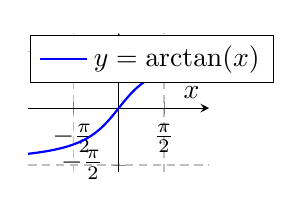
\begin{tikzpicture}
		\begin{axis}[axis lines=middle,xlabel={$x$},ylabel={$y$},
			width=0.32\textwidth,
			trig format plots=rad,
			samples=101,
			unbounded coords=jump,
			xmin=-pi,xmax=pi,
			ymin=-pi/2-0.2,ymax=pi/2+0.5,
			xtick={-pi/2,pi/2},xticklabels={$-\frac{\pi}{2}$,$\frac{\pi}{2}$},
			%ytick={-pi/2,pi},yticklabels={$-\frac{\pi}{2}$,$\frac{\pi}{2}$},
			ytick={-pi/2,pi/2},yticklabels={$-\frac{\pi}{2}$,$\frac{\pi}{2}$},
			grid=major,grid style={densely dashed},
			legend style={at={(0.01,0.99)},anchor=north west}
			]
			\addplot[blue,thick,variable=\t,domain=-pi/2+0.1:pi/2-0.1] ({tan(\t)},\t);
			\addlegendentry{$y=\arctan(x)$}
			%\addplot[red,dashed,thick,variable=\t,domain=-10:10] (\t,{atan(\t)});
			%\addplot[green!60!black,variable=\t,domain=-pi/2+0.1:pi/2-0.1] ({cot(\t)},\t);
			%\addplot[green!60!black,variable=\t,domain=-0.0+0.1:pi-0.1] ({cot(\t)},\t);
			%\draw[green!60!black,dashed] (0,-2) -- (0,2);
			%\addlegendentry{$y=\text{arccot}(x)$}
		\end{axis}
	\end{tikzpicture}

	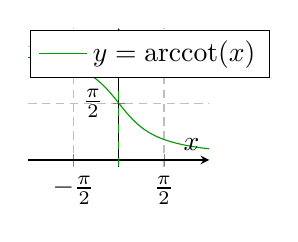
\begin{tikzpicture}
	\begin{axis}[axis lines=middle,xlabel={$x$},ylabel={$y$},
		width=0.32\textwidth,
		trig format plots=rad,
		samples=101,
		unbounded coords=jump,
		xmin=-pi,xmax=pi,
		ymin=-0.0-0.2,ymax=pi+0.5,
		xtick={-pi/2,pi/2},xticklabels={$-\frac{\pi}{2}$,$\frac{\pi}{2}$},
		%ytick={-pi/2,pi},yticklabels={$-\frac{\pi}{2}$,$\frac{\pi}{2}$},
		ytick={0.0, pi/2, pi},yticklabels={$0.0$,$\frac{\pi}{2}$, $\pi$},
		grid=major,grid style={densely dashed},
		legend style={at={(0.01,0.99)},anchor=north west}
		]
		%\addplot[green!60!black,variable=\t,domain=-pi/2+0.1:pi/2-0.1] ({cot(\t)},\t);
		\addplot[green!60!black,variable=\t,domain=-0.0+0.1:pi-0.1] ({cot(\t)},\t);
		\draw[green!60!black,dashed] (0,-2) -- (0,2);
		\addlegendentry{$y=\text{arccot}(x)$}
	\end{axis}
\end{tikzpicture}
	%\caption{``Standard'' branches of the multivalued functions $\arctan$ and $\text{arccot}$.}
%\end{figure}

%If someone really wanted to, one can try to cover $\mathbb{R}^2$ with another polar coordinate chart, but I would argue that we already have the cartesian coordinate chart that singlely covers $\mathbb{R}^2$. Also note that the transition map between polar coordinate charts and the cartesian coordinate chart is easy, since the cartesian chart is the identity.  

Let's try to cover $\mathbb{R}^2$ as much as possible with these "polar coordinate"-type charts. Unfortunately, we'll find out that we can't cover the origin in a well-defined (meaning with one-to-one functions) manner, so we'll have to consider $\mathbb{R}^2\backslash 0 := \mathbb{R}^2 - \lbrace 0 \rbrace$ (the Euclidean space $\mathbb{R}^2$ but without the origin).

Repeat some of the steps we did above. Consider open subset 
\[
U_+ = \lbrace (x, y) | x > 0 \text{ or } y \neq 0 \rbrace
\]
obtained by considering
\[
\begin{aligned}
& V_+ = \lbrace (r, \varphi) | r >0, \, \varphi \in (-\pi, \pi) \rbrace \in \mathbb{R}^2 \\
& [0, \infty) \times (-\pi, \pi] - V_+ = \lbrace (r, \varphi) | r = 0 \text{ or } \varphi = \pi \rbrace
\end{aligned}
\]
Consider if $\varphi = \pi$. Then $\begin{aligned} & \quad \\
	& x = -r \\
	& y = 0 \end{aligned}$ \, for $r> 0$, so $x<0 $ and $y=0$. If $r=0$, then $(x, y) = (0,0)$. So $\varphi^{-1}_{\text{pol}, +}(V_+) = \lbrace ( x, y) | x > 0 \text{ or } y\neq 0 \rbrace$

\begin{equation} \label{Eq:UR22}
	\begin{gathered}
		(U_+, \varphi_{\text{pol},+}) \in \mathcal{A} \\ 
		\begin{aligned}
			U_+ & = \lbrace (x,y) | x>0 \text{ or } y \neq 0 \rbrace  \\
			\varphi_{\text{pol}, +}(U) & = \lbrace (r,\varphi) | r >0, \varphi \in (-\pi,\pi) \rbrace
		\end{aligned} \\
	 \begin{aligned}
			& \varphi_{\text{pol},+}:U_+ \to \mathbb{R}^2 \backslash 0 \\ 
			& \varphi_{\text{pol},+}(x,y) = ( \sqrt{x^2 + y^2}, \begin{cases} \arctan{ \left( \frac{y}{x} \right) }  & \text{ if } (x > 0 \text{ and } y \geq 0 ) \text{ or } (x > 0 \text{ and } y \leq 0) \\ \arctan{ \left( \frac{y}{x} \right) } + \pi & \text{ if } ( x \leq 0 \text{ and } y > 0)) \\
			\arctan{ \left( \frac{y}{x} \right) } - \pi & \text{ if } (x\leq 0 \text{ and } y < 0) \end{cases} ) \\ 
			& \varphi^{-1}_{\text{pol},+}: \varphi_{\text{pol},+}(U) \to \mathbb{R}^2\backslash 0 \\ 
			& \varphi^{-1}_{\text{pol},+}(r,\varphi) = (r\cos{\varphi}, r\sin{\varphi}) = (x,y)
		\end{aligned}
	\end{gathered}
\end{equation}
where $\pi/ 2 < \arctan(x) < \pi/ 2$, with limits $\lim_{x \to -\infty} \arctan(x) = -\pi/2$ and $\lim_{x \to \infty} \arctan(x) = \pi/2$ being well defined.



\subsection{Spheres}

cf. Example 1.4 (Spheres), Lee (2012) \cite{JLee2012}, pp. 5

$\forall \, n \geq 0, \, n \in \mathbb{Z}$, $n$-sphere $\mathbb{S}^n$ is Hausdorff and second-countable because it's topological subspace of $\mathbb{R}^{n+1}$. \\
$\forall \, i = 1, \dots n +1$, let $U_i^+ = \lbrace (x^1, \dots x^{n+1}) \in \mathbb{R}^{n+1}: x^i > 0 \rbrace$. \\
Similarly, let $U_i^- = \lbrace (x^1, \dots x^{n+1})  \in \mathbb{R}^{n+1} : x^i < 0 \rbrace$  \\

Let $f: \mathbb{B}^n \to \mathbb{R}$ be $f(u) = \sqrt{ 1 - |u|^2}$. \\

$\forall \, i =1 , \dots n +1$, $U_i^+ \cap \mathbb{S}^n$ is graph of function
\[
x^i = f(x^1 \dots \widehat{x}^i \dots x^{n+1})
\]

where $\widehat{x}^i$ indicates $x^i$ is omitted, \\
since
\[
\sqrt{ (x^1)^2  + (x^{n+1})^2 } = 1^2 \text{ or } (x^i)^2 = 1 - \sum_{ \substack{ j\neq i \\ i =1} }^{n+1} (x^j)^2 \Longrightarrow x^i = f(x^1, \dots \widehat{x}^i, \dots x^{n+1})
\]

Similarly, $U_i^i \cap \mathbb{S}^n$ is graph of 
\[
x^i = -f(x^1 \dots \widehat{x}^i \dots x^{n+1})
\]
sicne $x^i < 0$.

Thus, $\forall \,$ subset $U_i^{\pm} \cap \mathbb{S}^n$ is locally Eucliean of dim. $n$ nad maps
\[
\begin{aligned}
	& \varphi_i^{\pm} : U_i^{\pm} \cap \mathbb{S}^n \to \mathbb{B}^n \\
	& \varphi_i^{\pm} (x^1 \dots x^{n+1}) = (x^1 \dots \widehat{x}^i \dots x^{n+1})
\end{aligned}
\]
are graph coordinates for $\mathbb{S}^n$.

Since $\forall \,$ pt. $\in \mathbb{S}^n$ is in domain of at least 1 of these $2n+2$ charts, $\mathbb{S}^n$ is a topological $n$-manifold.

cf. Example 1.31 (Spheres), Lee (2012) \cite{JLee2012}, pp. 20, \\

$\forall \, i = 1 \dots n+1$, let $(U_i^{\pm}, \varphi_i^{\pm})$ denote graph coordinate charts, s.t.

\[
\begin{aligned}
	& U_i^{\pm} = \lbrace (x^1 \dots x^{n+1}) \in \mathbb{R}^{n+1} : x^i \gtrless 0 \rbrace \\ 
	& \varphi_i^{\pm} : U_i^{\pm} \cap \mathbb{S}^n \to \mathbb{B}^n \\ 
	& \varphi_i^{\pm} (x^1 \dots x^{n+1}) = (x^1, \dots \widehat{x}^i \dots x^{n+1})
\end{aligned}\]

$\forall \, $ distinct $i,j$, transition map $\varphi_i^{\pm} \circ (\varphi_j^{\pm})^{-1}$ is computed; for $i<j$,
\[
\varphi_i^{\pm} \circ (\varphi_j^{\pm})^{-1} (u^1 \dots u^n) = (u^1, \dots \widehat{u}^i \dots \pm \sqrt{1 - |u|^2}, \dots u^n )
\]

with $\sqrt{1- |u|^2}$ in $j$th position; similarly for $i =j$. \\

Also $\varphi_i^+ \circ (\varphi_i^-)^{-1} (x^1, \dots x^n) = \varphi_i^{+} (x^1 \dots - \sqrt{1 - \sum_i(x^i)^2} \dots x^n) = (x^1 \dots x^n)$. \\

So $\varphi_i^+ \circ (\varphi_i)^{-1} = \varphi_i^- \circ (\varphi_i^+)^{-1} = 1_{\mathbb{B}^n}$. \\

$\lbrace (U_i^{\pm}, \varphi_i^{\pm}) \rbrace$ is a smooth atlas, defines smooth structure on $\mathbb{S}^n$. This is its \textbf{standard smooth structure}.


\problemhead{1, Wald (1984) \cite{Wald1984}}
\begin{enumerate}
	\item[(a)] In Wald's notation, $f^+_i : O_i^+ \to D$; compare Lee's notation against Wald's, respectively:
	
	\[
	\varphi_i^{\pm} : U^{\pm}_i \cap S^n \to \mathbb{B}^n \equiv f_i^{\pm} : O_i^{\pm} \to D^n
	\]
	
	\[
	\varphi_i^{\pm} \circ (\varphi_j^{\pm})^{-1} (x^1 \dots x^n) = \varphi_i^{\pm}( x^1, \dots \pm \sqrt{ 1 -\sum_{k=1}^n (x^k)^2} \dots x^n) = (x^1 \dots \widehat{x}^i \dots \pm \sqrt{ 1 - \sum_{k=1}^n (x^k)^2 } , \dots x^n)
	\]
Clearly, $\varphi_i^{\pm} \circ (\varphi_j^{\pm})^{-1}$ is $C^{\infty}$ by taking $\frac{ \partial}{\partial x^k} $ to any order, since $\mathbb{B}^n$ doesn't include its boundary.

	\item[(b)] See \emph{stereographic projection}: 

	\textbf{north pole} $N = (0, \dots 0, 1) \in S^n \subseteq \mathbb{R}^{n+1}$ \\
\textbf{south pole} $S = (0, \dots 0,-1) \in S^n \subseteq \mathbb{R}^{n+1}$ \\
\textbf{stereographic projection} 
\[
\begin{aligned}
	& \sigma : \mathbb{S}^n \setminus \lbrace N \rbrace \to \mathbb{R}^n \\
	& \sigma(x^1 , \dots x^{n+1}) = \frac{ (x^1, \dots x^n ) }{ 1 - x^{n+1}} 
\end{aligned}
\]
\[
\begin{aligned}
	& \widetilde{\sigma}: \mathbb{S}^n \setminus \lbrace S \rbrace \to \mathbb{R}^n \\
	& \widetilde{\sigma}(x^1 , \dots x^{n+1}) = -\sigma(-x) = \frac{ x^1, \dots x^n }{ 1 + x^{n+1}}
\end{aligned}
\]

\end{enumerate}

\problemhead{1-7, Lee (2012) \cite{JLee2012}, \textbf{Stereographic projection of spheres}}

Let $N$ denote the \textbf{north pole} $(0, \dots, 0, 1) \in \mathbb{S}^n \subseteq \mathbb{R}^{n+1}$, and let S denote the \textbf{south pole} $(0, \dots , 0 , -1)$. Define the \textbf{stereographic projection} $\sigma: \mathbb{S}^n \setminus \lbrace N \rbrace \to \mathbb{R}^n$ by 
\[
\sigma(x^1, \dots x^{n+1}) = \frac{ (x^1, \dots x^n ) }{ 1 - x^{n+1}}
\]
Let $\widetilde{\sigma}(x) = -\sigma(-x)$ for $x\in \mathbb{S}^n \setminus \lbrace S \rbrace$.

\begin{enumerate}
	\item[(a)] So given a \\
	\textbf{north pole} $N = (0, \dots 0, 1) \in S^n \subseteq \mathbb{R}^{n+1}$ \\
	\textbf{south pole} $S = (0, \dots 0,-1) \in S^n \subseteq \mathbb{R}^{n+1}$ \\
	\textbf{stereographic projection} 
	\[
	\begin{aligned}
		& \sigma : \mathbb{S}^n \setminus \lbrace N \rbrace \to \mathbb{R}^n \\
		& \sigma(x^1 , \dots x^{n+1}) = \frac{ (x^1, \dots x^n ) }{ 1 - x^{n+1}} 
	\end{aligned}
	\]
	\[
	\begin{aligned}
		& \widetilde{\sigma}: \mathbb{S}^n \setminus \lbrace S \rbrace \to \mathbb{R}^n \\
		& \widetilde{\sigma}(x^1 , \dots x^{n+1}) = -\sigma(-x) = \frac{ x^1, \dots x^n }{ 1 + x^{n+1}}
	\end{aligned}
	\]

Consider $\mathbf{x} \in \mathbb{S}^n \setminus \lbrace N \rbrace \to \mathbb{R}^n$, $\mathbf{x} = (x^1 \dots x^{n+1})$.
\[
\begin{gathered}
	N + t(\mathbf{x} - N) = \mathbf{x}' \Longrightarrow 1 + t(x^{n+1} - 1 ) = 0 \text{ or } t = \frac{1}{ 1- x^{n+1}} \\
	(x')^i = \frac{x^i}{ 1 - x^{n+1}}  \quad \, \forall \, i \neq n + 1
\Longrightarrow \sigma(x^1 \dots x^{n+1}) = \frac{ (x^1, \dots x^n) }{ 1 - x^{n+1}}
\end{gathered}
\]
Thus we have a stereographic projection from the north pole.

\[
\begin{gathered}
	S + t(\mathbf{x} - S) = \mathbf{x}' \Longrightarrow 1 + t(x^{n+1} + 1) = 0 \text{ or } t= \frac{1}{1 + x^{n+1}} \\
	(x')^i = \frac{x^i }{ 1 + x^{n+1}} \quad \, \forall \, i \neq n + 1 \\
	\Longrightarrow \widetilde{\sigma}(x^1 \dots x^{n+1}) = \frac{ (x^1, \dots x^n) }{ 1 + x^{n+1}}
\end{gathered}
\]
\textbf{Thus we have a stereographic projection from the south pole}.

\item[b]
\[
\begin{gathered}
\begin{aligned}
	& \sigma^{-1} (u^1 \dots u^n) = \frac{(2u^1 \dots 2u^n, |u|^2 - 1) }{ |u|^2 + 1 } \\
	& \sigma \circ \sigma^{-1}(u^1 \dots u^n) = \frac{ (2u^1 \dots 2u^n) }{ |u|^2 + 1 } / \left( 1 - \frac{ |u|^2 - 1 }{ |u|^2 + 1 } \right) = (u^1, \dots u^n)
\end{aligned}	\\
\sigma^{-1} \circ \sigma(x^1, \dots x^{n+1}) = \sigma^{-1} \frac{ (x^1 \dots x^n) }{ 1 - x^{n+1} } = \frac{ \left(\frac{ 2 x^1}{ 1 - x^{n+1} } , \dots \frac{2x^n}{1 - x^{n+1} } , \frac{ (x^1)^2 + \dots + (x^n)^2 }{ ( 1- x^{n+1})^2 } - 1 \right) }{ \frac{ (x^1)^2 + \dots + (x^n)^2}{ (1- x^{n+1})^2 } + 1 } = \\
= \frac{ \left( \frac{ 2 x^1}{ 1 - x^{n+1}} \dots \frac{2x^n}{1- x^{n+1}} , \frac{ (x^1)^2 + \dots + (x^n)^2 }{ (1-x^{n+1})^2} - \frac{ 1 - 2x^{n+1} + (x^{n+1})^2 }{ (1- x^{n+1})^2} \right) }{ \frac{2(1-x^{n+1})}{(1-x^{n+1})^2} } = \left( x^1, \dots x^n , \frac{ 1 - (x^{n+1})^2 - 1 + 2x^{n+1} - (x^{n+1})^2 }{ \frac{ 2 }{ 1 - x^{n+1}} (1- x^{n+1})^2 } \right) = \\
= (x^1, \dots x^n , \frac{2 x^{n+1} ( 1 -x^{n+1}) }{ \frac{ 2 }{ 1 - x^{n+1}} ( 1 - x^{n+1})^2 } ) = (x^1, \dots x^{n+1})
\end{gathered}
\]
\item[(c)] Compute the transition map $\widetilde{\sigma} \circ \sigma^{-1}$. (The coordinates defined by $\sigma$ or $\widetilde{\sigma}$ are called \textbf{stereographic coordinates}).

\[
\begin{gathered}
	\widetilde{\sigma} \circ \sigma^{-1}(u^1 \dots u^n) = \widetilde{\sigma} \frac{(2u^1 \dots 2u^n, |u|^2-1) }{ |u|^2 +  1} = \frac{ \frac{2u^1}{ |u|^2 + 1} , \dots \frac{2u^n}{ |u|^2 + 1} }{ 1 + \frac{ |u|^2 - 1 }{ |u|^2 + 1} } = \frac{ \frac{2u^1}{ |u|^2 + 1} , \dots \frac{2u^n}{ |u|^2 + 1} }{  \frac{2|u|^2}{ |u|^2 + 1} } = \\
	= \boxed{ \left( \frac{u^1}{ |u|^2} , \dots , \frac{u^n}{ |u|^2} \right) }
\end{gathered}
\]

\end{enumerate}

\subsubsection{Polar coordinates}

Consider 
\[
\mathbf{x}(\theta, \varphi) = (s\theta c\varphi, s\theta s\varphi, c\theta)
\]
\[
\begin{aligned}
& \theta = \arccos{z}, \quad \, \theta \in [0, \pi] , \, z \in [0,1] \\
& \begin{gathered}
\varphi = \begin{cases}
	& \arctan{ \left( \frac{y}{x} \right) } \text{ if } x > 0, \, \varphi \in ( \frac{-\pi}{2}, \frac{\pi}{2}) \\
	& \arctan{ \left( \frac{y}{x} \right) }  + \pi if x < 0 \text{ and } y > 0, \, \varphi \in (\frac{\pi}{2}, \pi) \\
	& \arctan{ \left( \frac{y}{x} \right) }  - \pi if x < 0 \text{ and } y < 0, \, \varphi \in (-\pi, \frac{-\pi}{2}) \\ 
	& \frac{\pi}{2} \text{ if } x = 0, y = 1\\
	& \frac{-\pi}{2} \text{ if } x= 0 , y = -1
\end{cases}	
\end{gathered}
\end{aligned}
\]


\section{Inverse Function Theorem}

Shastri (2011) had a thorough and lucid and explicit explanation of the Inverse Function Theorem \cite{AShastri2011}.  I will recap it here.  The following is also a blend of Wienhard's Handout 4 \url{https://web.math.princeton.edu/~wienhard/teaching/M327/handout4.pdf}

\begin{definition}
  Let $(X,a)$ metric space.  

\textbf{contraction} $\phi:X \to X$ if $\exists \, $ constant $0<c<1$ s.t. $\forall \, x,y \in X$
\[
d(\phi(x),\phi(y)) \leq cd(x,y)
\]
\end{definition}

\begin{theorem}[Contraction Mapping Principle]
  Let $(X,d)$ complete metric space.  \\
Then $\forall \, $ contraction $\phi:X\to X$, $\exists \, ! y\in X$ s.t. $\phi(y) = y$, $y$ \emph{fixed pt.}
\end{theorem}

\begin{proof}
  Recall def. of complete metric space $X$, $X$ metric space s.t. $\forall \, $ Cauchy sequence in $X$ is convergent in $X$ (i.e. has limit in $X$).  

$\forall \, x_0 \in X$,
Define $\begin{aligned} & \quad \\
  & x_1 = \phi(x_0) \\ 
  & x_2 = \phi(x_1) \\ 
  & \vdots \\
  & x_j = \phi(x_{j-1}) \\ 
  & \vdots \\
  & x_n = \phi(x_{n-1})
\end{aligned}$

\[
\begin{gathered}
  d(x_{n+1},x_n) = d(\phi(x_n),\phi(x_{n-1})) \leq c d(x_n,x_{n-1}) \leq \dots \leq c^nd(x_1,x_0)
\end{gathered}
\]
for some $0< c<1$.

\[
d(x_m,x_n) \leq d(x_n,x_{n-1}) + d(x_{n-1},x_m) \leq d(x_n,x_{n-1}) + d(x_{n-1},x_{n-2}) + \dots + d(x_{m+1},x_m) \leq \sum_{k=n-1}^m c^k d(x_1,x_0)
\]
Thus, $\forall \, \epsilon >0$, $\exists \, n_0 >0$, ($n_0$ large enough) s.t. $\forall \, m ,n\in \mathbb{N}$ s.t. $n_0 < n <m$, 
\[
d(x_m,x_n) \leq \sum_{k=n-1}^m c^k d(x_1,x_0) < \epsilon d(x_1,x_0)
\]
Thus, $\lbrace x_n \rbrace$ Cauchy sequence.  Since $X$ complete, $\exists \, $ limit pt. $y \in X$ of $\lbrace x_n \rbrace$.  
\[
\phi(y) = \phi(\lim_n x_n) = \lim_n \phi(x_n) = \lim_n x_{n+1} = y
\]
Since by def. of $y$ limit pt. of $\lbrace x_n \rbrace$, $\forall \, \epsilon >0$, then $\lbrace n | |x_n -y|\leq \epsilon, \, n \in \mathbb{N}\rbrace$ is infinite.  

Consider $\delta > \mathbb{N}$.  Consider $\lbrace n | |x_n-y| \leq \delta, n \in \mathbb{N}\rbrace$ 

$\exists \, N_{\delta} \in \mathbb{N}$ s.t. $\forall \, n > N_{\delta}$, $|x_n-y|< \delta$; otherwise, $\forall \, N_{\delta}$, $\exists \, n > N_{\delta}$ s.t. $|x_n - y| \geq \delta$.  Then $\lbrace n | |x_n -y| \leq \delta , n \in \mathbb{N} \rbrace$ finite.  Contradiction.  

$\phi$ cont. so by def. $\forall \, \epsilon >0$, $\exists \, \delta >0$ s.t. if $|x_n -y| < \delta$, then $|\phi(x_n) - \phi(y) | < \epsilon$.  

Pick $N_{\delta}$ s.t. $\forall \, n > N_{\delta}$, $|x_n-y| < \delta$, and so $|\phi(x_n) - \phi(y)|< \epsilon$. There are infinitely many $\phi(x_n)$'s that satisfy this, and so $\phi(y)$ is a limit pt.  

If $\exists \, y_1,y_2 \in X$ s.t. $\begin{aligned} & \quad \\
  & \phi(y_1) = y_1 \\ 
  & \phi(y_2) = y_2 \end{aligned}$, then
\[
d(y_1,y_2) = d(\phi(y_1), \phi(y_2)) \leq c d(y_1,y_2) \text{ with } c <1
\]
so $c=1$
\end{proof}


\begin{theorem}[Inverse Function Theorem]
  Suppose open $U \subset \mathbb{R}^n$, let $C^1 \, f: U \to \mathbb{R}^n$, $x_0 \in U$ s.t. $Df(x_0)$ invertible.  

%  Let open $E \subset \mathbb{R}^n$, $0 \subset E$, let $f \in \mathcal{C}^1(E,\mathbb{R}^n)$ s.t. $Df(0)$ invertible.  

Then $\exists \,$ open neighborhoods $V\ni x_0$, $W \ni f(x_0)$ s.t. $V\subseteq U$ and $W\subseteq \mathbb{R}^n$, respectively, and s.t.

\begin{enumerate}
\item[(i)] $f: V\to W$ bijection
\item[(ii)] $g = f^{-1}:V \to U$ differentiable, i.e. $g = f^{-1}:W\to V$ is $C^1$
\item[(iii)] $D(f^{-1}) $ cont. on $W$.  
\item[(iv)] $Dg(y) = (Df(g(y)))^{-1}$ \, $\forall \, y \in W$
\end{enumerate}
Also, notice that $f(g(y)) = y \, \forall \, y \in W$.  
\end{theorem}

\begin{proof}
%  Let $A = Df(0)$, consider $\widehat{f} = A^{-1}\circ f$.  Then $\widehat{f} \in (U;\mathbb{R}^n)$.  $D(\widehat{f})(0)=1$ since $D(\widehat{f})(0) = D(A^{-1} \circ f)(0)=A^{-1}Df(0)=1$.  

Consider $\widetilde{f}(x) = (Df(x_0))^{-1}(f(x+x_0) - f(x_0))$.  Then \\
\phantom{Consider} $\widetilde{f}(0) = 0$ and 
\[
\begin{aligned}
  &  D\widetilde{f}= (Df(x_0))^{-1}(Df(x+x_0) -0)  \\
  & D\widetilde{f}(0) = (Df(x_0))^{-1}Df(x_0)=1
\end{aligned}
\]  
So let $\widetilde{f}\to f$ (notation) and so assume, without loss of generality, that $U\ni 0$, $f(0)=0$, $Df(0)=1$

Choose $0 < \epsilon \leq \frac{1}{2}$.  Let $0< \delta <1$ s.t. open ball $V = B_{\delta}(0) \subseteq U$, and $\| Df(x)-1\| < \epsilon$.  $\forall \, x \in U$, since $Df$ cont. at $0$.  

Let $W=f(V)$.  

$\forall \, y \in W$, define $\begin{aligned} & \quad \\
  & \phi_y : V \to \mathbb{R}^n \\
  & \phi_y(x) = x + (y-f(x))\end{aligned}$

\[
\begin{aligned}
  & D(\phi_y)(x) = 1 + - Df(x) \quad \, \forall \, x \in V \\ 
  & \| D(\phi_y)(x) \| = \| 1 - Df(x) \| \leq \epsilon <1
\end{aligned}
\]

$\forall \, x_1 ,x_2 \in V$, by mean value Thm. (not the equality that is only valid in 1-dim., but the inequality, that's valid for $\mathbb{R}^d$, 
\[
\| \phi_y(x_1) - \phi_y(x_2) \| \leq \| D(\phi_y)(x') \| \| x_1 - x_2 \| 
\]
for some $x' = cx_2 + (1-c)x_1$, $c\in [0,1]$.  $V$ only needed to be convex set.  
\[
\Longrightarrow \| \phi_y(x_1) - \phi_y(x_2) \| \leq \epsilon \| x_1 - x_2 \|
\]
Then $\phi_y$ contraction mapping.  

Suppose $f(x_1) = f(x_2)=y$, $x_1,x_2 \in V$.  
\[
\begin{gathered}
\begin{aligned}
  & \phi_y(x_1) =x_1 \\ 
  & \phi_y(x_2) =x_2  
\end{aligned} \\
\| \phi_y(x_1) - \phi_y(x_2) \| = \| x_1 - x_2 \| \leq \epsilon \| x_1 - x_2 \| \quad \, \forall \, \epsilon > 0 \Longrightarrow x_1 = x_2 
\end{gathered}
\]
$\Longrightarrow \left. f\right|_U$ injective.

$W=f(V)$, so $f:V\to W$ surjective.  $f$ bijective.  

Fix $y_0 \in W$, $y_0 = f(x_0)$, $x_0 \in V$.  \\
Let $r>0$ s.t. $B_r(x_0) \subset V$.  \\
Consider $B_{r\epsilon}(y_0)$.  If $y\in B_{r\epsilon}(y_0)$.  
\[
\begin{gathered}
  r\epsilon > \| y-y_0 \| = \| y - f(x_0) \| = \| \phi_y(x_0) - x_0 \| \text{ with } \\
  \phi_y(x) = x + (y-f(x))
\end{gathered}
\]

If $x\in B_r(x_0)$, 
\[
\| \phi_y(x) -x_0 \| \leq \| \phi_y(x) - \phi_y(x_0) \|  + \| \phi_y(x_0) - x_0 \| \leq \epsilon \| x-x_0 \| + r\epsilon < 2 r\epsilon = r
\]

%Consider $B_{r\epsilon }(y_0)$.  

Thus $\phi(B_r(x_0)) = B_r(x_0)$.

By contraction mapping principle, $\exists \, a \in B_r(x_0)$, s.t. $\phi_y(a)=a$.  Then $\phi_y(a) = a+ (y-f(a)) = a \Longrightarrow f(a) =y$.  

$y\in f(V) = W$.  

So $B_{r\epsilon}(y_0) \subset W$.  $W$ open.  

Let $\text{Mat}(n,n) \equiv $ space of all $n\times n$ matrices; $\text{Mat}(n,n)  = \mathbb{R}^{n^2}$.  


\end{proof}

There is a proof of the implicit function theorem and its various forms in Shastri (2011) \cite{AShastri2011}, but I found Wienhard's Handout 4 for Math 327 to be clearer.\footnote{\url{https://web.math.princeton.edu/~wienhard/teaching/M327/handout4.pdf}}

\begin{theorem}[Implicit Function Theorem]
Let open $U \subset \mathbb{R}^{m+n} \equiv \mathbb{R}^m \times \mathbb{R}^n$  \\
\phantom{Let} $C^1 \, f:U \to \mathbb{R}^n $ \\
\phantom{Let} $(a,b) \in U$ s.t. $f(a,b) = 0$ and $\left. D_y f\right|_{(a,b)}$ invertible.  

Then $\exists \, $ open $V \ni (a,b)$, $V \subset U$ \\
\phantom{Then} $\exists \, $ open neighborhood $W \ni a$, $W \subseteq \mathbb{R}^m$ \\
\phantom{Then} $\exists \, !$ \, $C^1 \, g:W \to \mathbb{R}^n$ s.t.
\[
\lbrace (x,y) \in V | f(x,y) =0 \rbrace = \lbrace (x,g(x)) | x \in W \rbrace
\]
Moreover,
\[
dg_x = - \left. (d_yf)^{-1} \right|_{(x,g(x))} \left. d_x f\right|_{(x,g(x))}
\]
and $g$ smooth if $f$.  
\end{theorem}

\begin{proof}
  Define $\begin{aligned} & \quad \\
    & F: U \to \mathbb{R}^{m+n}   \\
    & F(x,y) = (x,f(x,y)) \end{aligned}$

Then $F(a,b) = (a,0)$ (given), and 
\[
DF = \left[ \begin{matrix} 1 & \\ 
    \frac{ \partial f^i(x,y)}{ \partial x^j} & \frac{ \partial f^i(x,y) }{ \partial y^j } \end{matrix} \right] \equiv \left[ \begin{matrix} 1 & \\
    D_xf & D_yf \end{matrix} \right]
\]
$DF(a,b)$ invertible.  

By inverse function theorem, since $DF(a,b)$ invertible at pt. $(a,b)$, \\
$\exists \, $ open neighborhoods $\begin{aligned} & \quad \\
  & V \ni (a,b) \subseteq \mathbb{R}^m \times \mathbb{R}^n \\
  & \widetilde{W} \ni (a,0) \subseteq \mathbb{R}^m \times \mathbb{R}^n \end{aligned}$ s.t. $F$ diffeomorphism with $F^{-1}: \widetilde{W} \to V$. 

Set $W = \lbrace x \in \mathbb{R}^m | (x,0) \in \widetilde{W}\rbrace$.  Then $\pi_1(\widetilde{W}) =W$ open in $\mathbb{R}^m$.  

Define $g:W\to \mathbb{R}^n$, 
\[
\begin{aligned}
  & g(x) = \pi_2 \circ F^{-1}(x,0) \text{ or } \\ 
  & F^{-1}(x,0) = (h(x),g(x))
\end{aligned}
\]

Now $FF^{-1}(x,0) = (x,0) = (h(x), f(h(x),g(x)) )$ so $h(x)=x \, \forall \, x \in W$, $0 = f(x,g(x))$.  

Then
\[
\lbrace (x,y) \in V | f(x,y) = 0 \rbrace = \lbrace (x,y) \in V | F(x,y) = (x,0) \rbrace = \lbrace (x,g(x)) | x \in W, 0 = f(x,g(x)) \rbrace
\]
Since $\pi$ smooth and $F^{-1}$ is $C^1$, $g$ is $C^1$.  

To reiterate, $f(x,g(x)) =0$ on $W$.

Using chain rule while differentiating $f(x,g(x))=0$, 
\[
\begin{gathered}
\partial_{x^j} f(x,g(x)) = \frac{ \partial f(x,g(x)) }{ \partial x^k} \frac{ \partial x^k}{ \partial x^j}+ \frac{ \partial f(x,g(x))}{ \partial y^k}\frac{ \partial g^k(x)}{\partial x^j} = \left. D_x f \right|_{(x,g(x))} + \left. (D_yf) \right|_{(x,g(x))} \cdot (Dg)_x = 0 \text{ or }  \\
(Dg)_x = -\left. (D_yf) \right|_{x,g(x)} \left. D_xf \right|_{(x,g(x))}
\end{gathered}
\]



\end{proof}

\section{Immersions}

\begin{definition}[Immersion]
  smooth $f:M \to N$, s.t. $Df(p) : T_pM \to T_{f(p)}N$ injective.  Then $f$ \textbf{immersion} at $p$.  
\end{definition}

Absil, Mahony, and Sepulchre \cite{AMS2008} pointed out that another definition for a \emph{immersion} can utilize the theorem that $\text{rank}$ of $Df \equiv DF = \text{dim} T_pM$.  Indeed, recall these facts from linear algebra:  

for $T:V \to W$,  \\
It's always true that $\begin{aligned} & \quad \\ 
& \text{rank}T \leq V \\ 
& \text{rank}T \leq W \end{aligned}$, and \\

$\text{rank}T = \text{dim}V$ iff $T$ injective.  \\
$\text{rank}T = \text{dim}W$ iff $T$ surjective.  \\


\[
\begin{gathered}
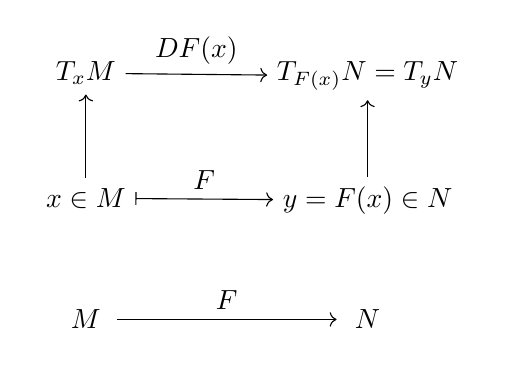
\begin{tikzpicture}
\matrix (m) [matrix of math nodes, row sep=2.8em, column sep=4.8em, minimum width=2.2em]
{
	T_xM & T_{F(x)}N = T_yN \\
	x \in M & y=F(x) \in N  \\ 
	M & N \\ 
};
\path[->]
(m-1-1) edge node [above] {$DF(x)$} (m-1-2)
(m-2-1) edge node [auto] {$$} (m-1-1)
(m-2-2) edge node [auto] {$$} (m-1-2)
(m-3-1) edge node [auto] {$F$} (m-3-2)
;
\path[|->]
(m-2-1) edge node [auto] {$F$} (m-2-2)
;
\end{tikzpicture}   \\
\end{gathered}
\]

Now 
\[
\begin{aligned}
& \text{dim}T_xM = \text{dim}M \\ 
& \text{dim}T_{F(x)}N = \text{dim}N 
\end{aligned}
\]
And 
\[
\text{rank}(DF(x)) \equiv \text{rank of $F$ }
\]
I know that the notation above is confusing, but this is what all Differential Geometry books apparently mean when they say "rank of $F$".  

Now  
\[
\text{rank}(DF(x)) = \text{dim}(\text{im}(DF(x)))  = \text{dim}T_xM \text{ iff } DF(x) \text{ injective }  
\]

If $\forall \, x \in M$, this is the case, then $F$ an \textbf{ immersion }.  

Apply the rank-nullity theorem in this case:  

\[
\begin{gathered}
	\text{rank}(DF(x)) + \text{dim}\text{ker}(DF(x)) = \text{dim}T_xM = \text{dim}M \\ 
	\Longrightarrow \text{rank}(DF(x)) = \text{dim}M \leq \text{dim}T_{F(x)}N = \text{dim}N \text{ or } \text{dim}M \leq \text{dim}N 
\end{gathered}
\]

Now 

\[
\text{rank}(DF(x)) = \text{dim}T_{F(x)}N \text{ iff } DF(x) \text{ surjective }  
\]

If $\forall \, x \in M$, this is the case, then $F$ an \textbf{ submersion }.  

\[
 \text{rank}(DF(x)) = \text{dim}T_{F(x)}N = \text{dim}N  \leq \text{dim}M  
\]

Shastri (2011) has this as the ``Injective Form of Implicit Function Theorem'', Thm. 1.4.5, pp. 23 and Guillemin and Pollack (2010) has this as the ``Local Immersion Theorem'' on pp. 15, Section 3 ``The Inverse Function Theorem and Immersions'' \cite{VGuilleminAPollack2010}.  

\begin{theorem}[Local immersion Theorem i.e. Injective Form of Implicit Function Theorem]\label{Thm:LocalImmersion}
  Suppose $f:M\to N$ immersion at $p$, $q=f(p)$.  

Then $\exists \, $ local coordinates around $p,q$, $x,y$, respectively s.t. $f(x_1\dots x_m) = (x_1 \dots x_m,0 \dots 0)$.  

\end{theorem}

\begin{proof}
  Choose local parametrizations 
\[
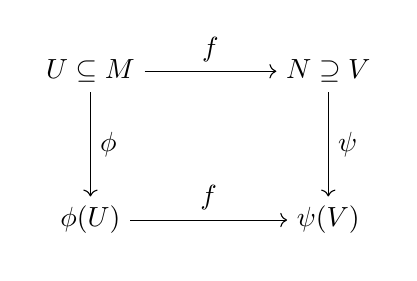
\begin{tikzpicture}
  \matrix (m) [matrix of math nodes, row sep=3.8em, column sep=4.8em, minimum width=2.2em]
  {
    U \subseteq M & N \supseteq V \\
    \phi(U) & \psi(V) \\
};
  \path[->]
  (m-1-1) edge node [above] {$f $} (m-1-2)
          edge node [auto] {$\phi$} (m-2-1)
  (m-1-2) edge node [auto]  {$\psi$} (m-2-2)
  (m-2-1) edge node [auto] {$f$} (m-2-2)
  ;
\end{tikzpicture}  
\quad \quad \, \begin{aligned} & \phi(p) = x \\
  & \psi(q) = y \end{aligned}
\]
$D(\psi f\varphi^{-1}) \equiv Df$.  $Df(p)$ injective (given $f$ immersion).  $Df(p) \in \text{Mat}(n,m)$

By change of basis in $\mathbb{R}^n$, assume $Df(p) = \left( \begin{matrix} I_m \\ 0 \end{matrix} \right)$.  

Now define $\begin{aligned} & \quad \\
  & G : \phi(U) \times \mathbb{R}^{n-m} \to \mathbb{R}^n \\
  & G(x,z) = f(x) + (0,z) \end{aligned}$

Thus, $DG(x,z) =1$ and for open $\phi(U) \times U_2$, $ G(\phi(U)\times U_2)$ open.  

By inverse function theorem, $G$ local diffeomorphism of $\mathbb{R}^n$, at $0$.  

Now $f = G\circ \mathfrak{i}$, where $\mathfrak{i}$ is canonical immersion.  
\[
\begin{gathered}
  G(x,0) = f(x) \\
  \Longrightarrow G^{-1}G(x,0) = (x,0) = G^{-1}f(x)
\end{gathered}
\]

Use $\psi \circ G$ as the local parametrization of $N$ around pt. $q$.  Shrink $U,V$ so that 

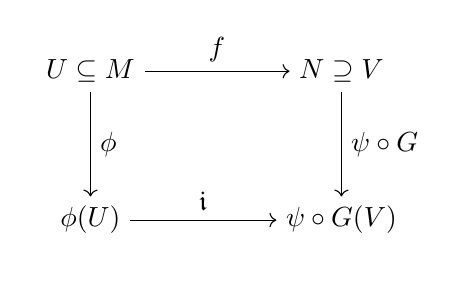
\begin{tikzpicture}
  \matrix (m) [matrix of math nodes, row sep=3.8em, column sep=4.8em, minimum width=2.2em]
  {
    U \subseteq M & N \supseteq V \\
    \phi(U) & \psi\circ G(V) \\
};
  \path[->]
  (m-1-1) edge node [above] {$f $} (m-1-2)
          edge node [auto] {$\phi$} (m-2-1)
  (m-1-2) edge node [auto]  {$\psi\circ G$} (m-2-2)
  (m-2-1) edge node [auto] {$\mathfrak{i}$} (m-2-2)
  ;
\end{tikzpicture}  

\end{proof}






\begin{theorem}[Implicit Function Thm.]
  Let open subset $U\subseteq \mathbb{R}^n \times \mathbb{R}^d$, $(x,y) = (x^1 \dots x^n, y^1 \dots y^k) $ on $U$.  \\
  Suppose smooth $\Phi:U\to \mathbb{R}^k$, $(a,b) \in U$, $c=\Phi(a,b)$

  If $k\times k$ matrix $\frac{ \partial \Phi^i}{ \partial y^j}(a,b)$ nonsingular, then $\exists $ neighborhoods $\begin{aligned} & \quad \\
    & V_0 \subseteq \mathbb{R}^n \text{ of $a$ } \\
    & W_0 \subseteq \mathbb{R}^k \text{ of $b$ } \end{aligned}$ and smooth $F:V_0 \to W_0$ s.t.

  $\Phi^{-1}(c) \bigcap (V_0\times W_0)$ is graph of $F$, i.e. \\
  $\Phi(x,y) =c$ for $(x,y) \in V_0\times W_0$ iff $y=F(x)$.  
  \end{theorem}



\section{Submersions; Rank Theorem} 
cf. pp. 20, Sec. 4 "Submersions", Ch. 1 of Guillemin and Pollack (2010) \cite{VGuilleminAPollack2010}.  

Consider $X,Y\in \text{\textbf{Man}}$, s.t. $\text{dim}X \geq \text{dim}Y$.  

\begin{definition}[submersion] If $f:X\to Y$, \\
if $Df_x \equiv df_x$ is \emph{surjective}, $f\equiv $ \textbf{submersion} at $x$.
\end{definition}
Recall that,  
\[
\begin{gathered}
	Df_x:T_xX \to T_{f(x)}Y \\
	\text{dim}T_xX \geq \text{dim}T_{f(x)}Y
\end{gathered}
\]
\[
\begin{gathered}
\text{rank}Df_x \leq \text{dim}T_{f(x)}Y, \text{ in general, while } \\
\text{rank}Df_x = \text{dim}T_{f(x)}Y \text{ iff } Df_x \text{ surjective }
\end{gathered}
\]

Canonical submersion is standard projection: \\
If $\begin{gathered} \quad \\
\text{dim}X = k \\
\text{dim}Y = l \end{gathered}$, $k\geq l$, 
\[
(a_1 \dots a_k ) \mapsto (a_1 \dots a_l)
\]

\begin{theorem}[Local Submersion Theorem]\label{Thm:LocalSubmersion}
	Suppose $f:X\to Y$ submersion at $x$, and $y = f(x)$, 
	Then $\exists \, $ local coordinates around $x$, $y$ s.t. 
	\[
	f(x_1\dots x_k) = (x_1 \dots x_l)
	\]
	i.e. $f$ locally equivalent to canonical submersion near $x$
\end{theorem}
\begin{proof}
I'll have a side-by-side comparison of my notation and the 1 used in Guillemin and Pollack (2010) \cite{VGuilleminAPollack2010} where I can.	

For charts $(U,\phi), (V,\psi)$ for $X,Y$, respectively, $y=f(x)$ for $x\in X$, 
\[
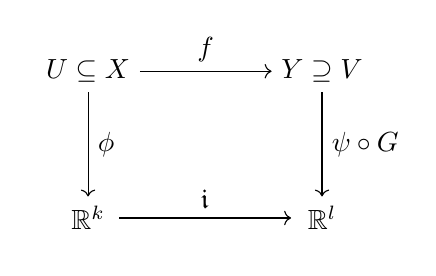
\begin{tikzpicture}
\matrix (m) [matrix of math nodes, row sep=3.8em, column sep=4.8em, minimum width=2.2em]
{
	U \subseteq X & Y \supseteq V \\
	\mathbb{R}^k &  \mathbb{R}^l \\
};
\path[->]
(m-1-1) edge node [above] {$f $} (m-1-2)
edge node [auto] {$\phi$} (m-2-1)
(m-1-2) edge node [auto]  {$\psi\circ G$} (m-2-2)
(m-2-1) edge node [auto] {$\mathfrak{i}$} (m-2-2)
;
\end{tikzpicture} \quad \quad \, 
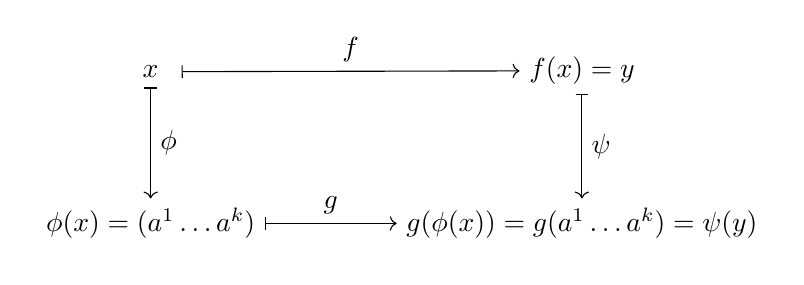
\begin{tikzpicture}
\matrix (m) [matrix of math nodes, row sep=3.8em, column sep=4.8em, minimum width=2.2em]
{
	 x & f(x)=y \\
	\phi(x)=(a^1\dots a^k) &  g(\phi(x))=g(a^1\dots a^k)=\psi(y) \\
};
\path[|->]
(m-1-1) edge node [above] {$f $} (m-1-2)
edge node [auto] {$\phi$} (m-2-1)
(m-1-2) edge node [auto]  {$\psi$} (m-2-2)
(m-2-1) edge node [auto] {$g$} (m-2-2)
;
\end{tikzpicture}
\]
$Dg_x$ surjective, so assume it's a $l\times k$ matrix $\left[ \begin{matrix} \mathbf{1}_l & 0 \end{matrix} \right]$.  

Define
\begin{equation}
\begin{aligned}
& G:U \subset \mathbb{R}^k \to \mathbb{R}^k  \\
& G(a)\equiv G(a^1\dots a^k) := (g(a), a_{l+1}, \dots , a_k)
\end{aligned}
\end{equation}
Now
\begin{equation}
DG(a)  = \left[ \begin{matrix} \mathbf{1}_l & 0 \\ & \mathbf{1}_{k-l} \end{matrix} \right] = \mathbf{1}_k
\end{equation}
so $G$ local diffeomorphism (at $0$).  

So $\exists \, $ $G^{-1}$ as local diffeomorphism of some $U'$ of $a$ into $U\subset \mathbb{R}^k$.  

By construction, 
\begin{equation}
g=\mathbb{P}_l \circ G
\end{equation}
where $\mathbb{P}_l$ is the \emph{canonical submersion}, the projection operator onto $\mathbb{R}^l$.  
\[
g\circ G^{-1} = \mathbb{P}_l
\]
(since $G$ diffeomorphism)

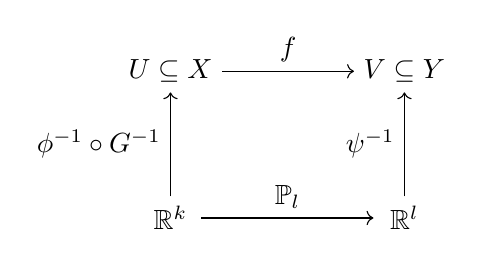
\begin{tikzpicture}
\matrix (m) [matrix of math nodes, row sep=3.8em, column sep=4.8em, minimum width=2.2em]
{
	U\subseteq X &  V\subseteq Y \\
	\mathbb{R}^k &  \mathbb{R}^l \\
};
\path[->]
(m-2-1) edge node [auto] {$\phi^{-1}\circ G^{-1}  $} (m-1-1)
edge node [auto] {$\mathbb{P}_l$} (m-2-2)
(m-1-1) edge node [auto]  {$f$} (m-1-2)
(m-2-2) edge node [auto] {$\psi^{-1}$} (m-1-2)
;
\end{tikzpicture}
for \\
$\Longrightarrow $ 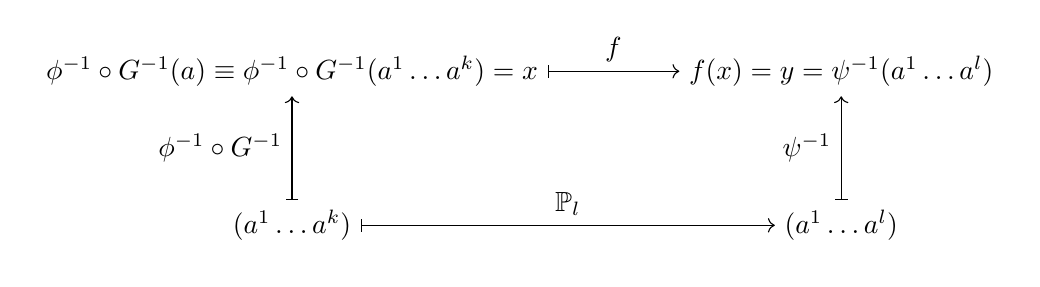
\begin{tikzpicture}
\matrix (m) [matrix of math nodes, row sep=3.8em, column sep=4.8em, minimum width=2.2em]
{
	\phi^{-1}\circ G^{-1}(a)\equiv \phi^{-1}\circ G^{-1}(a^1\dots a^k)=x & f(x)=y=\psi^{-1}(a^1\dots a^l) \\
	(a^1\dots a^k) &  (a^1\dots a^l) \\
};
\path[|->]
(m-2-1) edge node [auto] {$\phi^{-1}\circ G^{-1}  $} (m-1-1)
edge node [auto] {$\mathbb{P}_l$} (m-2-2)
(m-1-1) edge node [auto]  {$f$} (m-1-2)
(m-2-2) edge node [auto] {$\psi^{-1}$} (m-1-2)
;
\end{tikzpicture}


	\end{proof}
"An obvious corollary worth noting is that if $f$ is a submersion at $x$, then it is actually a submersion in a whole neighborhood of $x$." Guillemin and Pollack (2010) \cite{VGuilleminAPollack2010}

Suppose $f$ submersion at $x\in f^{-1}(y)$.  

By local submersion theorem
\[
f(x_1\dots x_k)=(x_1 \dots x_l)
\]
Choose $y=(0, \dots , 0)$. 

Then, near $x$, $f^{-1}(y) = \lbrace (0, \dots 0 , x_{l+1} \dots x_k)\rbrace$ i.e. let $V\ni x$ neighborhood of $x$, define $(x_1 \dots x_k)$ on $V$.  

Then $f^{-1}(y) \bigcap V = \lbrace (0\dots 0 , x_{l+1} , \dots x_k) | x_1 = 0 , \dots x_l = 0\rbrace$.

Thus $x_{l+1}, \dots x_k$ form a coordinate system on open set $f^{-1}(y) \bigcap V \subseteq f^{-1}(y)$.  

Indeed, 
\[
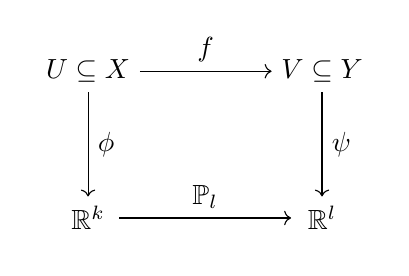
\begin{tikzpicture}
\matrix (m) [matrix of math nodes, row sep=3.8em, column sep=4.8em, minimum width=2.2em]
{
	U \subseteq X &  V\subseteq Y \\
	\mathbb{R}^k &  \mathbb{R}^l \\
};
\path[->]
(m-1-1) edge node [auto] {$ f  $} (m-1-2)
edge node [auto] {$ \phi $} (m-2-1)
(m-2-1) edge node [auto]  {$\mathbb{P}_l$} (m-2-2)
(m-1-2) edge node [auto] {$\psi$} (m-2-2)
;
\end{tikzpicture} \qquad \, 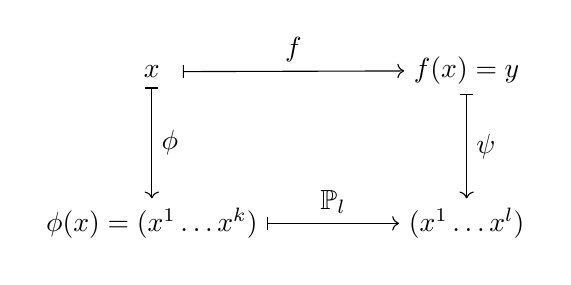
\begin{tikzpicture}
\matrix (m) [matrix of math nodes, row sep=3.8em, column sep=4.8em, minimum width=2.2em]
{
	x &  f(x)=y \\
	\phi(x)=(x^1\dots x^k) &  (x^1\dots x^l) \\
};
\path[|->]
(m-1-1) edge node [auto] {$ f  $} (m-1-2)
edge node [auto] {$ \phi $} (m-2-1)
(m-2-1) edge node [auto]  {$\mathbb{P}_l$} (m-2-2)
(m-1-2) edge node [auto] {$\psi$} (m-2-2)
;
\end{tikzpicture} 
\]
and now 
\[
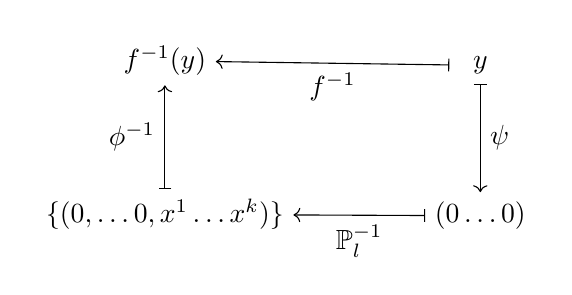
\begin{tikzpicture}
\matrix (m) [matrix of math nodes, row sep=3.8em, column sep=4.8em, minimum width=2.2em]
{
	f^{-1}(y) &  y \\
	\lbrace (0, \dots 0,x^1\dots x^k) \rbrace &  (0\dots 0) \\
};
\path[|->]
(m-1-2) edge node [auto] {$ f^{-1}  $} (m-1-1)
edge node [auto] {$ \psi $} (m-2-2)
(m-2-2) edge node [auto]  {$\mathbb{P}_l^{-1}$} (m-2-1)
(m-2-1) edge node [auto] {$\phi^{-1}$} (m-1-1)
;
\end{tikzpicture} 
\]

\subsection{Rank Theorem}

Lee (2012) \cite{JLee2012} in pp. 85, Ch. 4 Submersions, Immersions, and Embeddings, combines Theorems \ref{Thm:LocalImmersion}, \ref{Thm:LocalSubmersion} (local immersion and local submersion theorems, respectively) into the "Rank Theorem" (cf. Thm 4.12 "Rank Theorem" of Lee (2012)):

\begin{theorem}[Rank Theorem]
Suppose smooth manifolds $M, N$, $\text{dim}{M} = m$, $\text{dim}{N} = n$, smooth map $F:M \to N$, $F$ has constant rank $r$. \\
$\forall \, p \in M$, $\exists \, $ smooth charts $(U, \varphi)$ for $M$, centered at $p$, $(V, \psi)$ for $N$, centered at $F(p)$, s.t. 
\[
F(U) \subseteq V
\]
in which $F$ has coordinate representation of form
\begin{equation}
\widehat{F}(x^1 \dots x^r, x^{r+1} \dots x^m) = (x^1 \dots x^r , 0 \dots 0)
\end{equation}

Particularly, if $F$ smooth submersion,
\[
\widehat{F}(x^1 \dots x^n, x^{n+1} \dots x^m) = (x^1 \dots x^n)
\]

and if $F$ smooth immersion

\[
\widehat{F}(x^1 \dots x^m ) = (x^1 \dots x^m , 0 \dots 0)
\]
\end{theorem}

\[
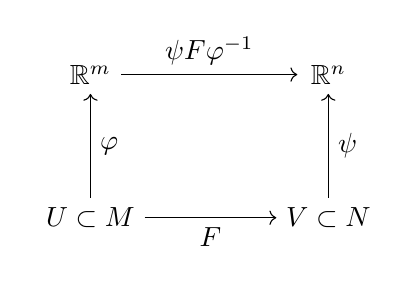
\begin{tikzpicture}
\matrix (m) [matrix of math nodes, row sep=3.8em, column sep=4.8em, minimum width=2.2em]
{
	\mathbb{R}^m &  \mathbb{R}^n \\
	U \subset M &  V \subset N \\
};
\path[->]
(m-1-1) edge node [above] {$ \psi F \varphi^{-1} $} (m-1-2)
(m-2-1) edge node [right] {$\varphi$} (m-1-1)
(m-2-1) edge node [below] {$F$} (m-2-2)
(m-2-2) edge node [right] {$\psi$} (m-1-2)
;
\end{tikzpicture}
\]
Also remember that $DF(p) : T_p M \to T_{F(p)}N$
\begin{proof}
	$DF(p)$ has rank $r$ (given). Then $DF(p)$ is some $r\times r$ submatrix of a $n\times m$ matrix s.t. $\text{det}DF(p)$ nonzero. 
	
	By change of basis in $\mathbb{R}^n$, or reordering coordinates, assume $DF(p)$ is upper left submatrix $\left( \frac{ \partial F^i}{ \partial x^j} \right) \quad \, \forall \, i,j = 1, \dots r$. 
	
	Relabel standard coordinate as 
	\[
	\begin{aligned} 
		& (x,y) = (x^1 \dots x^r, y^1 \dots y^{m-r})\in \mathbb{R}^m \\
		& (v,w) = (v^1 \dots v^r, w^1 \dots w^{n-r}) \in \mathbb{R}^n 
	\end{aligned}
	\]
	By initial translations of coordinates, assume without loss of generality $p = (0, 0)$, $F(p) = (0,0)$
	
	Suppose 
	\[
	F(x,y) = (Q(x,y) , R(x,y)) 
	\]
	for some smooth maps $Q : U\to \mathbb{R}^r$, $R:U\to \mathbb{R}^{n-r}$

	Define
	\[
	\begin{aligned}
	& \varphi : U \to \mathbb{R}^m \\ 
	& \varphi(x,y) = (Q(x,y), y)
	\end{aligned}
	\]
	so 
	\[
	D\varphi(0,0) = \left( \begin{matrix} \frac{ \partial Q^i }{ \partial x^j} (0,0) & \frac{ \partial Q^i }{ \partial y^j}(0,0) \\ 0 & \delta^i_j \end{matrix} \right) 
	\]
	$D\varphi(0,0)$ nonsingular, since $\text{det}\frac{\partial Q^i }{ \partial x^j} \neq 0$ (by hypothesis).
	
	By inverse function thm., $\exists \, $ connected neighborhoods $U_0$ of $(0,0)$, $\widetilde{U}_0$ of $\varphi(0,0) = (0,0)$ s.t. 
	\[
	\varphi : U_0 \to \widetilde{U}_0
	\]
	is a diffeomorphism.
	
	By shrinking $U_0, \widetilde{U}_0$, assume $\widetilde{U}_0$ open cube.
	
	Write $\varphi^{-1}(x,y) = (A(x,y), B(x,y))$, for some smooth functions $\begin{aligned} & \quad \\ 
	& A:\widetilde{U}_0 \to \mathbb{R}^r \\ 
	& B: \widetilde{U}_0 \to \mathbb{R}^{m-r}\end{aligned}$,
	\[
	(x,y) = \varphi(A(x,y) , B(x,y)) = (Q(A(x,y), B(x,y)), B(x,y))
	\]
	\[
	\Longrightarrow \begin{aligned} & B(x,y) = y \\ 
	& \varphi^{-1}(x,y) = (A(x,y), y) \end{aligned}  
	\]
	
	\[
	\varphi \varphi^{-1} = 1 \Longrightarrow x = Q(A(x,y), y)
	\]
	
	Recall that we had hypotehsized that 
	\[
	F(x,y) = (Q(x,y) , R(x,y))
	\]
	Then
	\[
	\begin{gathered}
		F \circ \varphi^{-1}(x,y) = F(A(x,y), y) = (Q(A(x,y), y), R(A(x,y), y)) = (x, R(A(x,y), y))
	\end{gathered}
	\]

	and so 
	\[
	F\circ \varphi^{-1}(x,y) = (x, \widetilde{R}(x,y))
	\]
	where $\begin{aligned} & \quad \\ 
	& \widetilde{R} : \widetilde{U}_0 \to \mathbb{R}^{n-r} \\
	& \widetilde{R}(x,y) = R(A(x,y), y)
	\end{aligned}$

	Compute
	\[
	\begin{gathered}
		D(F\circ \varphi^{-1})(x,y) = \left( \begin{matrix} \delta^i_j & 0 \\
		\frac{ \partial \widetilde{R}^i }{ \partial x^j}(x,y) & \frac{ \partial \widetilde{R}^i }{ \partial y^j}(x,y) \end{matrix} \right) 	
	\end{gathered}
	\]
	
	Since composing with a diffeomorphism doesn't change rank of map, $D(F\circ \varphi^{-1})$ has rank $r$ everywhere in $\widetilde{U}_0$.  

	$\left( \begin{matrix} \delta^i_j \\ \frac{ \partial \widetilde{R}^i }{ \partial x^j}(x,y) \end{matrix} \right)$ $j=1\dots r$ are linearly independent, so $\frac{\partial \widetilde{R}^i}{ \partial y^j}(x,y) = 0$ on $\widetilde{U}_0$, so $\widetilde{R}^i$ independent of $y^j$.
	
	Let $S(x) = \widetilde{R}(x,0)$, then
	\[
	F \circ \varphi^{-1}(x,y) = (x, S(x))
	\]
	Let open $V_0 \subseteq V$, $(0,0) \in V$ be an open subset $V_0 = \lbrace (v,w) \in V: (v,0) \in \widetilde{U}_0 \rbrace$. \\
	Then $V_0 $ is a neighborhood of $(0,0)$.
	
	Because $\widetilde{U}_0$ is a cube, $F \circ \varphi^{-1}(x,y) = (x, S(x))$,
	\[
	F\circ \varphi^{-1}(\widetilde{U}_0) \subseteq V_0
	\]
	so $F(U_0) \subseteq V_0$.
	
	Define $\begin{aligned} & \quad \\ 
	& \psi : V_0 \to \mathbb{R}^n \\
	& \psi (v,w) = (v, w- S(v)) \end{aligned}$
	
	Because $\psi^{-1}(s,t) = (s, t+S(s))$, \\
	it is a diffeomorphism.
	
	Thus $(V_0, \psi)$ is a smooth chart. 
	
	\[
	\psi \circ F (\varphi^{-1}(x,y)) = \psi(x, S(x)) = (x, S(x) - S(x)) = (x, 0)
	\]
	

	\end{proof}


\begin{definition}[regular value]
	For smooth $f:X\to Y$, $X,Y \in \text{\textbf{Man}}$, \\
	$y\in Y$ is a \textbf{regular value} for $f$ if $Df_x:T_xX \to T_y Y$ surjective $\forall \, x$ s.t. $f(x)=y$.  
	
	$y\in Y$ \textbf{critical value} if $y$ not a regular value of $f$.  
\end{definition}

Absil, Mahony, and Sepulchre \cite{AMS2008} pointed out that another definition for a \emph{regular value} can utilize the theorem that $\text{rank}$ of $Df \equiv DF = \text{dim} T_pN = \text{dim} N$, iff $DF(p)$ surjective, for $p\in M$, $F:M\to N$.  Then 

\textbf{regular value} $y \in N$, of $F$, if rank of $F \equiv \text{rank}(DF(x)) = \text{dim}N$, $\forall \, x \in F^{-1}(y)$, for $F:M\to N$.  


\begin{theorem}[Preimage theorem]
If $y$ regular value of $f:X\to Y$, \\
$f^{-1}(y)$ is a submanifold of $X$, with $\text{dim}f^{-1}(y)=\text{dim}X - \text{dim}Y$
\end{theorem}
\begin{proof}
Given $y$ is a regular value of $f:X\to Y$,  \\
$\forall \, x \in f^{-1}(y)$, $Df_x:T_xX \to T_yY$ is surjective.  By local submersion theorem, 
\[
f(x^1 \dots x^k) = (x^1 \dots x^l)=y
\]	
Since $x\in f^{-1}(y)$, $(x^1\dots x^k)=(y^1 \dots y^l,x^{l+1}\dots x^k)$.  

For this chart for $(U,\varphi)$, $U\ni x$, consider $(U\cap f^{-1}(y),\psi)$ with $\psi(x) = (x^{l+1}\dots x^k) \quad \, \forall \, x\in U\cap f^{-1}(y)$.  

$\forall \, f^{-1}(y)$ submanifold with $\text{dim}f^{-1}(y) = k-l = \text{dim}X-\text{dim}Y$.  
	\end{proof}

\emph{Examples for emphasis}

If $\text{dim}X > \text{dim}Y$, \\
\phantom{\qquad \, } if $y\in Y$, regular value of $f:X\to Y$, \\
\phantom{\qquad \, \qquad \, } $f$ submersion, $\forall \, x \in f^{-1}(y)$ \\
If $\text{dim}X = \text{dim}Y$, \\
\phantom{\qquad \, } $f$ local diffeomorphism $\forall \, x\in f^{-1}(y)$ \\
If $\text{dim}X < \text{dim}Y$, $\forall \, y\in f(X)$ is a critical value.  


\textbf{Example: $O(n)$ as a submanifold of $\text{Mat}(n,n)$}

Given $\text{Mat}(n,n)\equiv M(n) = \lbrace n \times n \text{ matrices } \rbrace$ is a manifold; in fact $\text{Mat}(n,n) \cong \mathbb{R}^{n^2}$, \\
Consider $O(n) = \lbrace A \in \text{Mat}(n,n) | AA^T = 1\rbrace$.  
\begin{equation}
AA^T \in \text{Sym}(n) \equiv S(n) = \lbrace S\in \text{Mat}(n,n) | S^T = S \rbrace = \lbrace \text{ symmetric $n\times n$ matrices } \rbrace
\end{equation}
$\text{Sym}(n)$ submanifold of $\text{Mat}(n,n)$, $\text{Sym}(n)$ diffeomorphic to $\mathbb{R}^k$ (i.e. $\text{Sym}(n) \cong \mathbb{R}^k$), $k:= \frac{n (n+1)}{2}$.  

\[
\begin{aligned}
	& f:\text{Mat}(n,n) \to \text{Sym}(n) \\
	& f(A) = AA^T
\end{aligned}
\]
Notice $f$ is smooth, 
\[
\begin{gathered}
f^{-1}(1) = O(n) \\
Df_A(B) = \lim_{s\to 0} \frac{ f(A+sB) - f(A) }{s} = \lim_{s\to 0} \frac{(A+sB)(A^T + sB^T)- AA^T}{s} = AB^T +BA^T
\end{gathered}
\]
If $Df_A : T_A\text{Mat}(n,n) \to T_{f(A)}\text{Sym}(n)$ surjective when $A\in f^{-1}(1) = O(n)$ (???).  





\begin{proposition} If smooth $g_1\dots g_l \in C^{\infty}(X)$ on $X$ are independent $\forall \, x\in X$, s.t. $g_i(x)=0$, $\forall \, i = 1\dots l$, \\
	then $Z=\lbrace x\in X | g_1(x) = \dots = g_l(x)=0 \rbrace = $ set of "common zeros" is a \emph{submanifold} of $X$ s.t. $\text{dim}Z = \text{dim}X- l$.  
	
	Take \emph{note} that $g_1 \dots g_l$ are independent at $x$ means, really, that $D(g_1)_x \dots D(g_l)_x$ are linearly independent on $T_xX$.  
\end{proposition}
\begin{proof}
Suppose smooth $g_1 \dots g_l \in C^{\infty}(X)$ on manifold $X$ s.t. $\text{dim}X = k\geq l$.  

Consider $g=(g_1\dots g_l):X \to \mathbb{R}^l$, $Z\equiv g^{-1}(0)$.  

Since $\forall \, g_i$ smooth, $D(g_i)_x:T_xX \to \mathbb{R}$ linear.  

Now for 
\[
Dg_x = (D(g_1)_x \dots D(g_l)_x):T_xX \to \mathbb{R}^l
\]	
By rank-nullity theorem (linear algebra), $Dg_x$ surjective iff $\text{rank}Dg_x = l$ i.e. $l$ functionals $D(g_1)_x \dots D(g_l)_x$ are linearly independent on $T_xX$.  

"We express this condition by saying the $l$ functions $g_1\dots g_l$ are independent at $x$."  (Guillemin and Pollack (2010) \cite{VGuilleminAPollack2010})  
	
	
	\end{proof}

\section{Submanifolds; immersed submanifold, embedded submanifolds, regular submanifolds}  

\begin{definition}[Embedded Submanifold]
	
\end{definition}

Recall immersion:  \\
$F:M \to N$ immersion iff $DF$ injective, i.e. iff $\text{rank}DF = \text{dim}M$.  

Consider manifolds $M\subseteq N$.  \\
Consider inclusion map $\begin{aligned} & \quad \\ 
	& i:M\to N \\
	& i: x \mapsto x \end{aligned}$.  
	
	If $i$ immersion, $Di(x) = \frac{\partial y^i}{ \partial x^j} = \delta_j^{\  \  i}$ if $y^i = x^i$, $\forall \, i =1,\dots \text{dim}M$.  
	
\begin{definition}[immersed submanifold]
	\textbf{immersed submanifold} $M \subseteq N$ if inclusion $i:M\to N$ is an immersion.  
\end{definition}	
cf. 3.3 Embedded Submanifolds of Absil, Mahony, and Sepulchre \cite{AMS2008}, also Ch. 5 Submanifolds, pp. 108, \textbf{Immersed Submanifolds} of  John Lee (2012) \cite{JLee2012}.  

Immersed submanifolds often arise as images of immersions.  

\begin{proposition}[Images of Immersions as submanifolds]
	Suppose smooth manifold $M$, \\
	\phantom{Suppose } smooth manifold with or without boundaries $N$, \\
	injective, smooth immersion $F:M\to N$ ($F$ injective itself, not just immersion)  
	
Let $S=F(M)$.  

Then $S$ has unique topology and smooth structure of smooth submanifolds of $N$ s.t. $F:M\to S$ diffeomorphism.  
	
\end{proposition}
cf. Prop. 5.18 of John Lee (2012) \cite{JLee2012}.  

\begin{proof}
Define topology of $S$: set $U\subseteq S$ open iff $F^{-1}(U) \subseteq M$ open ($F^{-1}(U\cap V) = F^{-1}(U) \cap F^{-1}(V), F^{-1}(U\cup V) =F^{-1}(U) \cup F^{-1}(V)$).  \\
Define smooth structure of $S$: $\lbrace F(U), \varphi \circ F^{-1}  | (U,\varphi) \in \text{atlas for $M$, i.e. $(U,\varphi)$ any smooth chart of $M$}\rbrace$.  

"smooth compatibility condition": 
\[
(\varphi_2\circ F^{-1}) (\varphi_i F^{-1})^{-1} = \varphi_2 \circ F^{-1}F\varphi_1^{-1} = \varphi_2 \varphi_1^{-1}
\]
since $\varphi_2\varphi_1^{-1}$ diffeomorphism ($\varphi_2 \varphi_1^{-1}$ bijection and it and inverse is differentiable) 

$F$ diffeomorphism onto $F(M)$.  

	and these are the only topology and smooth structure on $S$ with this property: 
	\[
	S \xrightarrow{F^{-1}} M \xrightarrow{F} N \qquad \, = \qquad \, S \hookrightarrow M
	\]
	and $F^{-1}$ diffeomorphism, $F$ smooth immersion, so $i : S \to M$ smooth immersion.  
	\end{proof}

\section{Curves, Integral Curves, and Flows}

cf. John Lee (2012) \cite{JLee2012}, Ch. 9, deals with time-dependent vector fields and I don't see other texts or references handling such an important, but overlooked, case.

\subsection{Curves in Euclidean space}

cf. 4.1 Jeffrey Lee (2009) \cite{JLee2009}

If $C$ is 1-dim. submanifold of $\mathbb{R}^n$, $p\in C$, $\exists \, $ chart $(V, y)$ of $C$, $p\in V$ s.t. $y(V)$ is a connected open interval $I \subset \mathbb{R}$, \\
inverse map $y^{-1} : I \to V \subset M$ is a local parametrization. \\
idea is to extract information that's appropriately independent of parametrization. \\

If $\gamma : I \to \mathbb{R}^n$, $c: J \to \mathbb{R}^n$ curves with same image, \\
$c$ is a \textbf{positive reparametrization} of $\gamma$ if $\exists \, $ smooth $h: J \to I$ with $h' > 0 $ s.t. $c = \gamma \circ h$, \\
in this case, $\gamma, c$ have same \textbf{sense} and same \textbf{orientation}. \\

Assume $\gamma : I \to \mathbb{R}^n$ has $\| \gamma' \| >0$, \\
Such a curve is \textbf{regular}, i.e. curve is an immersion (Recall, an immersion would be smooth $\gamma : I \to \mathbb{R}^n$, s.t. $D\gamma(p): T_p I \to T_{\gamma(p)}\mathbb{R}^n$ injective).  

\begin{definition}[unit tangent field in Euclidean space, 4.3 Lee (2009) \cite{JLee2009}]	
	If $\gamma:I \to \mathbb{R}^n$ regular curve, then $\mathbf{T}(t) := \frac{\gamma'(t)}{ \| \gamma'(t) \| }$ defines \textbf{unit tangent field} along $\gamma$ ($\|T \| = 1$)
\end{definition}

\textbf{length of a curve} defined on closed interval $\gamma :[t_1, t_2] \to \mathbb{R}^n$, 
\[
L  = \int_{t_1}^{t_2} \| \gamma'(t) \| dt
\]
Define \textbf{arc length function} for curve $\gamma:I \to \mathbb{R}^n$ by choosing $t_0 \in I$, 
\[
s = h(t) :=  \int_{t_0}^{t} \| \gamma'(t) \| d\tau
\]

If curve is smooth and regular, then $h'= \| \gamma'(\tau) \| >0$, so by inverse function theorem, $\exists \,$ smooth $h^{-1}$ (since $h'$ invertible (with $1/h'$)). 

If $c(s) = \gamma h^{-1}(s)$, then $\| c' \|(s) := \| c'(s)\| = 1$, \, $\forall \, s$
\[
\begin{gathered} 
c'(s) = (\gamma(h^{-1}(s)))' = \gamma'(h^{-1}(s)) \cdot \frac{dh^{-1}}{ds}(s) \\
\| c'(s) \| = \| \gamma'(t) \| \| \frac{dh^{-1}}{ds} (s) \| = h' \cdot \frac{1}{h'} = 1
\end{gathered} 
\]
Curves parametrized by arc length are \textbf{unit speed curves}.


For a unit speed curve, $\frac{dc}{ds}(s) = \mathbf{T}(s)$. 

\begin{definition}[curvature vector, curvature function, principal normal in Euclidean space, 4.4 Lee (2009) \cite{JLee2009}]
	Let $c:I \to \mathbb{R}^n$ be a unit speed curve. vector valued function
	\[
	\mathbf{\kappa}(s) := \frac{d\mathbf{T}}{ds}(s) 
	\]
	is called the \textbf{curvature vector}.
	
	\[
	\kappa(s) := \| \mathbf{\kappa}(s) \| = \| \frac{d\mathbf{T}}{ds}(s) \|
	\]
	is called the \textbf{curvature function}.

	If $\kappa(s) >0$, then define principal normal
	\[
	\mathbf{N}(s) = \| \frac{d\mathbf{T}}{ds}(s) \|^{-1} \frac{d\mathbf{T}}{ds}(s) 
	\]
	s.t. $\frac{d\mathbf{T}}{ds} = \kappa \mathbf{N}$
\end{definition}

\subsection{Integral Curves}

cf. Ch. 9 of Lee (2012) \cite{JLee2012}

integral curves - smooth curves whose velocity at each point is equal to the value of the smooth vector field there. 

Let smooth manifold $M$ with or without boundary. \\
If smooth curve $\gamma : J \to M$, then $\forall \, t \in J$, velocity vector $\gamma'(t)$ is a vector in $T_{\gamma(t)}M$.  \\

\begin{definition}[Integral Curve $\Gamma$]
Integral curve: $\mathbf{v}, \gamma$. \\
If vector field $\mathbf{v}$ on $M$, \\
\textbf{integral curve} of $\mathbf{v}$ is differentiable curve $\gamma : J \to M$, whose velocity $\forall \, p \in M$, $V_{\gamma(t)}$
\[
\gamma'(t) = V_{\gamma(t)}, \, \forall \, t \in J
\]
\end{definition}

Finding integral curves boils downs to solving a system of ordinary differential equations in a smooth chart. \\
Suppose smooth vector field $V$ on $M$, smooth curve $\gamma : J \to M$ \\
On smooth coordinate domain $U \subseteq M$, \\
Write $\gamma$ in local coordinates as 
\[
\begin{gathered}
	\gamma(t) = (\gamma^{1}(t), \dots , \gamma^{n}(t)) \\
	\gamma^i(t) = x^i \circ \gamma(t) \text{ where } x^i : U \subseteq M \to \mathbb{R} 
\end{gathered}
\]

Then condition for $\gamma$ to be an integral curve.
\[
\gamma'(t) \equiv \dot{\gamma}(t) = V_{\gamma(t)}
\]
can be written as 
\[
\dot{\gamma}^i(t) \left. \frac{\partial}{\partial x^i} \right|_{\gamma(t)} = V^i(\gamma(t)) \left. \frac{\partial }{ \partial x^i } \right|_{\gamma(t)}
\]

which reduces to an autonomous system of ordinary differential equations (ODEs)

\begin{equation}
\begin{aligned} 
& \dot{\gamma}^1(t) = V^1(\gamma^1(t), \dots, \gamma^n(t)) \\ 
& \vdots \\ 
& \dot{\gamma}^n(t) = V^n(\gamma^1(t), \dots , \gamma^n(t))
\end{aligned} 
\end{equation}

20200306 EY: I use this notation which is more useful for me, e.g. taking the double derivative of the curve $\gamma$: 
\[
\begin{gathered} 
\begin{aligned} 
& \dot{\gamma}(t) = v(\gamma(t)) \in T_{\gamma(t)}U \\ 
& \dot{\gamma}(t) = v^i(\gamma^1(t), \dots, \gamma^n(t))
\end{aligned} \\ 
\frac{d}{dt} \dot{\gamma}^i(t) = \frac{d}{dt} v^i(\gamma^1(t), \dots , \gamma^n(t)) = \frac{d}{dt} v^i(x^1 , \dots , x^n) \\
= \frac{\partial v^i}{\partial x^j}(x) \dot{x}^j = \dot{\gamma}^j \frac{\partial \dot{\gamma}^i}{\partial x^j}
\end{gathered} 
\]

\section{Vector Bundle}

See Sec. 7.1 The definitions in Renteln (2014) \cite{Rent2014}.

\begin{definition}[Vector Bundle]
\textbf{vector bundle} $(E,M,Y,\pi)$ over manifold $M$ is manifold $E$, projection map $\pi:E \to M$ s.t. (3 axioms)
\begin{enumerate}
\item (\emph{All fibers are isomorphic}) $\forall \, $ fiber $\pi^{-1}(p)$, $p\in M$ is isomorphic to fixed vector space $Y$ of dim. $m$ ($m$ is rank of vector bundle)
\item (manifold $E$ is locally a product) $\forall \, p \in M$, $\exists \, $ neighborhood $U\ni p$ and diffeomorphism
\begin{equation}\label{Eq:VectorBundleTotalSpaceIsLocalProduct}
\varphi_U: \pi^{-1}(U) \to U\times Y
\end{equation}
($\varphi_U$ called \textbf{local trivialization} of $E$ over $U$)
\item (local trivialization $\varphi_U$ carries fibers to fibers and restriction is linear) 
\begin{equation}
\varphi_U: \pi^{-1}(p) \to \pi^{-1}_1(p)
\end{equation}
is linear $\forall \, p$. $\pi_1: U\times Y \to U$ is a projection onto first factor $(p,g) \mapsto p$
\end{enumerate}

Manifold $E$ is called \textbf{total space} or \textbf{bundle space}, manifold $M$ is called \textbf{base space}, $\pi$ bundle projection of vector bundle $(E,M,Y,\pi)$.
\end{definition}

Suppose $U,V$ are 2 overlapping neighborhoods of $p$ on $M$. Then we get
\begin{equation}
\begin{aligned}
& \varphi_V \circ \varphi_U^{-1} : (U \cap V) \times Y \to (U \cap V) \times Y \\
& (\varphi_V \circ \varphi_U^{-1}) (p, y_U) = (p, y_V)
\end{aligned}
\end{equation}
where $y_v= g_{VU}(p) y_U$ for some nondegenerate endomorphism $g_{VU}(p) : Y \to Y$ that varies smoothly with $p$. Endomorphism $g_{VU}$ is called \textbf{bundle transition} function.

TODO: Show this endomorphism $g$ explicitly:
\[
\begin{gathered}
\varphi_U^{-1}: (U \cap V) \times Y \to \pi^{-1}(U \cap V) \\
\varphi_U^{-1}: (p, y) \mapsto e \\
\varphi_V(e) \mapsto (p, y_V)
\end{gathered}
\]

\begin{corollary}
These so-called \textbf{cocycle conditions} are true:
\begin{equation}
\begin{aligned}
& g_{UU}(p) = 1 \\
& g_{UV}(p) g_{VU}(p) = 1 \\
& g_{UV}(p) g_{VW}(p) g_{WU}(p) = 1
\end{aligned}
\end{equation}
\end{corollary}

\begin{proof}
\begin{enumerate}
\item $\varphi_U \circ \varphi_U^{-1}: U\times Y \to U\times Y$ \\
$\varphi_U \circ \varphi_U^{-1} =1$. So $1:(p,y) \mapsto (p, y)$ and so $y = g_{UU}(p) y \Longrightarrow g_{UU}(p) = 1$.
\item $(\varphi_V \circ \varphi_U^{-1}) (p,y_U) = (p, y_V) $ s.t. $y_V = g_{VU}(p) y_U$. \\

$(\varphi_U \circ \varphi_V^{-1}) (p,z_V) = (p, z_U) $ s.t. $z_U = g_{UV}(p) z_V$. \\
\[
\begin{gathered}
(\varphi_U\circ \varphi_V^{-1}) (p, y_V) = (\varphi_U\circ \varphi_V^{-1}) (\varphi_V\circ \varphi_U^{-1}) (p, y_U) = 1 (p, y_U) = (p, g_{UV}(p) g_{VU}(p) y_U) \Longrightarrow g_{UV}(p) g_{VU}(p) = 1
\end{gathered}
\] Likewise,
\item \[
\begin{aligned}
& (\varphi_U \circ \varphi_V^{-1}) (p, y_V) = (p, g_{UV}(p) y_V) \\
& (\varphi_V \circ \varphi_W^{-1}) (p, y_W) = (p, g_{VW}(p) y_W) \\
& (\varphi_W \circ \varphi_U^{-1}) (p, y_U) = (p, g_{WU}(p) y_U) \\
\end{aligned}
\] and so
\[
\begin{gathered}
(\varphi_U \circ \varphi_V^{-1}) (\varphi_V \circ \varphi_W^{-1})(\varphi_W \circ \varphi_U^{-1}) (p, y_U) = (p, g_{UV}(p)g_{VW}(p)g_{WU}(p)y_U) = 1 (p, y_U)
\end{gathered}
\]
so $g_{UV}(p)g_{VW}(p)g_{WU}(p) = 1$
\end{enumerate}
\end{proof}

\begin{definition}[(vector bundle) section]
(smooth) section of $E$ is smooth map 
\begin{equation}
s : M \to E
\end{equation}
s.t. $\pi \circ s=1$
\end{definition}
This definition implies that $s$ is a vector-valued map (EY: $\pi^{-1}(p) \simeq $ vector space $Y$ so for $p \in M$, $s(p) = (y_1, y_2, \dots y_m) = (s_1(p), s_2(p), \dots s_m(p))$.

\section{Push-forward, Pull-back}

\subsection{Push-forward in coordinates, $f_*  : T_p M \to T_{f(p)}N$}

Using Nakahara (2003) \cite{Naka2003}'s notation.

Consider a smooth mapping $\begin{aligned} & \quad \\ 
		& f : M \to N \\
		& f_* : T_p M \to T_{f(p)}N \end{aligned}$, $\text{dim}M = m, \text{dim}N = n$.
	
With
\[
\begin{gathered}
\begin{aligned}
	& (U, \varphi) \subset M \\
	& (V, \psi) \subset N
\end{aligned} \quad \, \begin{aligned}
& \varphi: U \to \mathbb{R}^m \\
& \psi: V \to \mathbb{R}^n 
\end{aligned} \quad \, \begin{aligned}
& \varphi^i \equiv x^i : U \to \mathbb{R} \\ 
& \psi^j \equiv y^j : V \to \mathbb{R} 
\end{aligned}
\end{gathered}
\]

Now $\begin{aligned} & \quad \\ 
	& X \in T_p M \\ 
	& Y \in T_{f(p)} N \end{aligned}$, so we can write $\begin{aligned} & \quad \\ 
	& X = X^i \frac{\partial }{ \partial x^i} \\ 
	& Y = Y^j \frac{ \partial }{ \partial y^j } \end{aligned}$, \, and $f_* X \in T_{f(p)}N$, so we can write $f_* X = Y^j \frac{\partial }{ \partial y^j}$. \\

Let $\begin{aligned} & \quad \\ 
	 & g\in \mathcal{F}(N) \\
	 & g: N \to \mathbb{R} \end{aligned}$ \\
 
Now $g\circ \psi^{-1} : \mathbb{R}^n \to \mathbb{R}$ or $g \circ \psi^{-1} : \psi(N) \to \mathbb{R}$. \\

For notation, let $g\circ \psi^{-1} (y) \equiv g(y)$, in that we treat $y$ to be a point with coordinates in $\mathbb{R}^n$ notation-wise, and not as $y^j : V \to \mathbb{R}$. \\

Since $g\circ f: M \to \mathbb{R}$, so $g\circ f \in \mathcal{F}(M)$.
\begin{equation}\label{Eq:PushForwardCoordinateDerivation}
\begin{gathered}
\begin{aligned}
& (f_* X)[g] \equiv X[g \circ f] \\
& (f_* X)[g] = (Y^j \frac{\partial}{\partial y^j})[g] = Y^j \frac{\partial g}{ \partial y^j} = X^i \frac{\partial}{\partial x^i} [g \circ f] = X^i \frac{\partial}{\partial x^i} g(f^j(x)) = X^i \frac{\partial g}{ \partial y^j}(y) \frac{\partial f^j}{ \partial x^i}(x) = X^i \frac{\partial f^j}{ \partial x^i}(x) \frac{\partial}{\partial y^j} g
\end{aligned} \\
Y^j = X^i \frac{ \partial f^j}{\partial x^i} = X^i \frac{ \partial y^j}{\partial x^i} = F^j_{\, \, i}(x)X^i
\end{gathered}
\end{equation}
where $f:M \to N$, but $\psi \circ f \circ \varphi^{-1} : \varphi(U) \subset \mathbb{R}^m \to \mathbb{R}^n$, but write this notation as $f^j(x) = y^j$. \\

Also, notice that for Eq. \ref{Eq:PushForwardCoordinateDerivation},
\[
\begin{gathered}
	g\circ f: M \to \mathbb{R} \\
	g\circ \psi^{-1} \circ \psi \circ f \circ \varphi^{-1} \text{ and } g\circ f \circ \varphi^{-1} : \varphi(U) \subset \mathbb{R}^m \to \mathbb{R} \\
	(g\circ \psi^{-1}) (\psi \circ f \circ \varphi^{1}) (x) \equiv g(y(x))
\end{gathered}
\]

\subsection{Pullback in coordinates, $f^* : T^*_{f(p)}N \to T^*_pM$ } 

For pullback $f^* : T^*_{f(p)}N \to T^*_pM$, \\
since $\omega \in T^*_{f(p)}N$, then write as $\omega_j dy^j$ \\
since $f^*\omega \in T^*_pM$, so $f^* \omega = \psi_i dx^i$ 

\[
\begin{gathered}
\langle f^* \omega, X \rangle \equiv f^* \omega(X) = \langle \psi_i dx^i, X^j \frac{\partial }{ \partial x^j} \rangle \equiv \psi_i dx^i (X^j \frac{ \partial }{ \partial x^j} ) = \psi_i X^i = \langle \omega , f_* X \rangle  \equiv \omega(f_* X) = \\
= \langle \omega_j dy^j , Y^i \frac{ \partial }{ \partial y^i} \rangle = \omega_j dy^j ( Y^i \frac{\partial }{ \partial y^i} ) = \omega_j dy^j \left( X^i \frac{ \partial y^k}{ \partial x^i } \frac{ \partial }{ \partial y^k } \right) = \omega_j \frac{\partial y^i }{ \partial x^i } X^i 
\end{gathered}
\]
\[
\Longrightarrow \psi_i = \omega_j \frac{\partial y^j}{ \partial x^i}
\]

Thus
\begin{theorem}[Push-forward in coordinates] 
\[
\begin{gathered}
	\text{ For smooth } f: M \to N, \quad \,  \begin{aligned} & \text{dim}M = m \\ & \text{dim} N = n \end{aligned} \\
	\begin{aligned}
		& X = X^i \frac{\partial }{ \partial x^i} \in T_p M \\
		& Y = Y^j \frac{\partial }{ \partial y^j} \in T_{f(p)} N 		
	\end{aligned} \quad \, \text{ then }
\end{gathered} 
\]


\begin{equation}
	\boxed{
		\begin{gathered} 
\begin{aligned}
	& f_* : T_pM \to T_{f(p)} N \\
	& f_* (X) = Y 
\end{aligned} \quad \, \text{ s.t. } \\
Y^j = X^i \frac{\partial y^j}{\partial x^i} 
\end{gathered}
}
\end{equation}
where $f_*$ is the \textbf{push-forward}, and where colloquially, $y^j = y^j(x)$, but actually $y^j \equiv \psi \circ f \circ \varphi^{-1}$
\end{theorem} 

And

\begin{theorem}[Pullback in coordinates]
For smooth $f: M \to N$, \quad \, $ \begin{aligned} & \quad \\ 
	& \text{dim}M = m \\ 
	& \text{dim} N = n \end{aligned}$ \\ 
$\omega \in T^*_{f(p)}N$, $\psi = \psi_i dx^i \in T^*_pM$, then 

\begin{equation}
	\boxed{ 
\begin{gathered} 
\begin{aligned}
& f^* : T^*_{f(p)}N \to T^*_p M \\
& f^* \omega = \psi_i dx^i
\end{aligned} \quad \, \text{ where }  \\
\psi_i = \omega_j \frac{ \partial y^j}{ \partial x^i} 
\end{gathered}
}
\end{equation}	
\end{theorem} 

\section{Tensors}

I'll go through Ch.7 \emph{Tensors} of Jeffrey Lee (2009) \cite{JLee2009}.  

\begin{definition}[7.1\cite{JLee2009}] Let $V,W$ be modules over commutative ring $R$, with unity.  

Then, algebraic $W$-valued tensor on $V$ is multilinear map.  
\begin{equation}
	\tau: V_1 \times V_2 \times \dots \times V_m \to W
\end{equation}
where $V_i = \lbrace V,V^* \rbrace$ \quad \, $ \forall \, i=1,2,\dots m$.  

If for $r,s$ s.t. $r+s =m$, there are $r$ \, $V_i = V^*$, $s \, V_i = V$, tensor is $r$-contravariant, $s$-covariant; also say tensor of total type $\binom{r}{s}$.  
\end{definition}

EY : 20170404 Note that 
\[
\begin{aligned}
	& ( \tau_{\beta}^{i\alpha} \frac{ \partial }{ \partial x^i } \text{ or } \tau_{\beta}^{i\alpha} e_i )(\omega_j dx^j \text{ or } \omega_je^j  \in V^*) \\ 
	& ( \tau^{\beta}_{i\alpha} dx^i \text{ or } \tau^{\beta}_{i\alpha} e^i )( X^j \frac{ \partial }{ \partial x^j} \text{ or } X^j e_j  \in V) 
\end{aligned}
\]

$\exists \,$ natural map $\begin{aligned} & \quad \\ 
	& V\to V^{**} \\ 
& v \mapsto \widetilde{v} \end{aligned}$,  $\begin{aligned} & \quad \\ 
	& \widetilde{v} : \alpha \mapsto \alpha(v) \end{aligned}$.  If this map is an isomorphism, $V$ is \textbf{reflexive} module, and identify $V$ with $V^{**}$.  

\exercisehead{7.5} Given vector bundle $\pi: E \to M$, open $U\subset M$, consider sections of $\pi$ on $U$, i.e. cont. $s:U\to E$, where $(\pi\circ s)(u)=u$, \, $\forall \, u \in U$.  

Consider $E^* \ni \omega =\omega_i e^i$.  

$\forall \, s\in \Gamma(E)$, $\omega(s) = \omega_i(s(x))^i$, \, $\forall \, x \in U\subset M$.  So define $\widetilde{s}: \omega,x\mapsto \omega(s(x))$, \, $\forall \, x \in U$.  

If $\widetilde{s} =0$, $\widetilde{s}(\omega,x) = \omega(s(x)) =0$ \quad \, $\forall \, \omega \in E^*$, $\forall \, x\in U$, and so $s=0$.  (Let $\omega_i = \delta_{iJ}$ for some $J$, and so $s^J(x) =0$ \quad \, $\forall \, J$).  

$s=0$.  So $\text{ker}(s\mapsto \widetilde{s}) = \lbrace 0 \rbrace$ (so condition for injectivity is fulfilled).  

Since $\widetilde{s}:\omega,x\mapsto \omega(s(x))$, $\forall \, \omega \in E^*$, $\forall \, x \in U$, $s\mapsto \widetilde{s}$ is surjective.  

$s\mapsto \widetilde{s}$ is an isomorphism so $\Gamma(E)$ is a \emph{reflexive} module.  


\begin{proposition}
For $R$ a ring (special case), $\exists \, $ module homomorphism:  \\

tensor product space $\to $ tensor, as a multilinear map, i.e. $\exists$ \,  
\begin{equation}
\begin{aligned}
&	\left( \otimes_{i=1}^r V \right) \otimes \left( \otimes_{j=1}^s V^* \right) \to T^r_{ \, \, s}(V;R)   \\
& u_1 \otimes \dots \otimes u_r \otimes \beta^1 \otimes \dots \otimes \beta^s \in \left( \otimes^r V \right) \otimes \left( \otimes^s V^* \right) \mapsto (\alpha^1 \dots \alpha^r, v_1 \dots v_s) \mapsto \alpha^1(u_1) \dots \alpha^r(u_r) \beta^1(v_1) \dots \beta^s(v_s)  
\end{aligned}
\end{equation}
\end{proposition}

Indeed, consider 
\[
(\alpha^1 \dots \alpha^r, v_1 \dots v_s) \in \underbrace{V^* \times \dots \times V^* }_{r} \times \underbrace{ V\times \dots \times V}_{s} \mapsto \alpha^1(u_1) \dots \alpha^r(u_r) \beta^1(v_1) \dots \beta^s(v_s)
\]
and so for 
\[
\begin{aligned}
	& \alpha^i = \alpha^i_{\mu} e^{\mu} , \, & \, i =1,2, \dots r, \, & \, \mu = 1,2, \dots \text{dim}V^* \\ 
	& v_i = v_i^{\mu} e_{\mu} , \, & \, i = 1,2, \dots s, \, & \, \mu = 1, 2, \dots \text{dim}V 
\end{aligned} \qquad \, \begin{aligned}
& \alpha^i(u_i) = \alpha^i_{\mu} u^{\mu}_i \\ 
 & \beta^i(v_i) = \beta^i_{\mu} v^{\mu}_i
\end{aligned}
\]
So that 
\[
\begin{gathered}
	\alpha^1(u_1) \dots \alpha^r(u_r) \beta^1(v_1) \dots \beta^s(v_s) = \alpha^1_{\alpha_1}u^{\alpha_1}_1 \dots \alpha^r_{\alpha_r} u^{\alpha_r}_r \beta^1_{\mu_1} v^{\mu_1}_1 \dots \beta^s_{\mu_s} v^{\mu_s}_s = \\
	= (u^{\alpha_1}_1 \dots u_r^{\alpha_r} \beta^1_{\mu_1} \dots \beta^s_{\mu_s})(\alpha^1_{\alpha_1} \dots \alpha^r_{\alpha_r} v_1^{\mu_1} \dots v_s^{\mu_s} )
\end{gathered}
\]
Identify $u_1 \otimes \dots \otimes u_r \otimes \beta^1 \otimes \dots \otimes \beta^s$ with this multilinear map.  

\begin{proposition}
If $V$ is finite-dim. vector space, or if $V=\Gamma(E)$, for vector bundle $E\to M$, map
\begin{equation}
\left( \otimes_{i=1}^r V \right)  \otimes \left( \otimes_{j=1}^s V^* \right) \to T^r_{ \, \, s}(V;R)
\end{equation}
is an isomorphism.  
\end{proposition}

\begin{definition}
tensor that can be written as 
\begin{equation}
u_1\otimes \dots \otimes u_r \otimes \beta^1 \otimes \dots \otimes \beta^s \equiv u_1\otimes \dots \otimes \beta^s 
\end{equation}
is \textbf{simple} or \textbf{decomposable}.  
\end{definition}
Now well that not \emph{all} tensors are simple.  

\begin{definition}[7.7\cite{JLee2009}, tensor product]
$\forall \, S\in T^{r_1}_{ \,\, s_1}(V)$, $\forall \, T \in T^{r_2}_{ \,\, s_2}(V)$, \\
define tensor product 
\begin{equation}
\begin{gathered}
S\otimes T\in T^{r_1+r_2}_{ \, \, \, s_1+s_2}(V) \\
	S\otimes T( \theta^1\dots \theta^{r_1 + r_2}, v_1 \dots v_{s_1+s_2}) := S(\theta^1\dots \theta^{r_1}, v_1\dots v_{s_1})T(\theta^{r_1+1}\dots \theta^{r_1+r_2}, v_{s_1+1}\dots v_{s_1 + s_2} )
\end{gathered}
\end{equation}
\end{definition}

\begin{proposition}[7.8\cite{JLee2009}]
\end{proposition}







\[
\begin{gathered}
	\tau^{ i_1 \dots i_r }_{ \phantom{i_1 \dots i_r} j_1 \dots j_s} e_{i_1} \otimes \dots \otimes e_{i_r} \otimes e^{j_1}\otimes \dots \otimes e^{j_s} = \tau(e^{i_1} \dots e^{i_r}, e_{j_1} \dots e_{j_s} )e_{i_1} \otimes \dots \otimes e_{i_r} \otimes e^{j_1} \otimes \dots \otimes e^{j_s} = \tau 
\end{gathered}
\]
So $\lbrace e_{i_1}\otimes \dots \otimes e_{i_r} \otimes e^{j_1} \otimes \dots \otimes e^{j_s} | i_1 \dots i_{r}, j_1\dots j_s \in 1 \dots n \rbrace$ spans $T^r_{\,\, s}(V;R)$

\exercisehead{7.11}  Let basis for $V$ \, $e_1 \dots e_n$, corresponding dual basis for $V^*$ \,  $e^1 \dots e^n$ \\ 
Let basis for $V$ \, $\overline{e}_1 \dots \overline{e}_n$, corresponding dual basis for $V^*$ \,  $\overline{e}^1 \dots \overline{e}^n$ \\
s.t. 
\[
\begin{aligned}
	& \overline{e}_i = C^k_{ \,\, i} e_k \\
	& \overline{e}^i = (C^{-1})^i_{ \, \, k} e^k
\end{aligned}
\]
EY:20170404, keep in mind that
 
\[
\begin{aligned}
	&	Ax = e_i A^i_{ \, \, k} e^k(x^j e_j) = e_i A^i_{ \,\,j} x^j = A^i_{ \, \, j} x^j e_i \\ 
 & Ae_j = e_k A^k_{ \, \, i} e^i (e_j) = A^k_{ \,\, j} e_k = \overline{e}_j
\end{aligned}
\]
\[
\begin{gathered}
\overline{\tau}^i_{ \,\, jk} \overline{e}_i \otimes \overline{e}^j \otimes \overline{e}^k = \overline{\tau}^i_{ \, \, jk} C^l_{ \, \, i} e_l (C^{-1})^j_{ \,\, m} e^m(C^{-1})^k_{ \, \, n} e^n = \overline{\tau}^i_{ \, \, jk} C^l_{ \, \, i } (C^{-1})^j_{ \,\, m} (C^{-1})^k_{ \,\, n} = \tau^l_{ \,\, mn}   \\
\overline{\tau}^i_{ \,\, jk} = C^c_{ \,\, k} C^b_{ \,\, j} (C^{-1})^i_{ \,\, a} \tau^a_{\,\, bc}
\end{gathered}
\]



On Remark 7.13 of Jeffrey Lee (2009) \cite{JLee2009}:  first, egregious typo for $L(V,V)$; it shoudl be $L(V,W)$.  Onward, \\
for $L(V,W)$, \\
consider $W\otimes V^* \ni w\otimes \alpha$ s.t.
\[
(w\otimes \alpha)(v) = \alpha(v)w\in W, \, \forall \, v\in V, \text{ so } w\otimes \alpha \in L(V,W)
\]

Now consider (category of) left $R$-module, 
\begin{equation}
{\,}_R\textbf{Mod} \ni {\,}_{\text{Mat}_{\mathbb{K}}(N,M) } \mathbb{K}^N
\end{equation}
where
\[
\begin{aligned}
	& V=\mathbb{K}^N \\ 
&	  W = \mathbb{K}^M
\end{aligned}
\]
For $A\in \text{Mat}_{\mathbb{K}}(N,M)$, $x\in \mathbb{K}^N$, 
\[
e_i A^i_{ \,\ , \mu} e^{\mu}(x^{\nu} e_{\nu}) = Ax = e_iA^i_{\,\, \mu} x^{\mu} , \quad \, i=1,2,\dots M, \, \mu = 1,2, \dots N
\]
\[
A\in \text{Mat}_{\mathbb{K}}(N,M) \cong W\otimes V^* \cong L(V,W)
\]
Consider 
\[
\begin{aligned}
	& \alpha \in (\mathbb{K}^N)^* = V^* \\
	& w\in \mathbb{K}^M = W
\end{aligned} \qquad \, \begin{aligned}
	& \alpha = \alpha_{\mu} e^{\mu} \\ 
	& w=w^ie_i
\end{aligned}
\]
\[
\alpha \otimes w = w \otimes \alpha = w^i\alpha_{\mu} e_i \otimes e^{\mu}
\]
(remember, isomoprhism between $\text{Mat}_{\mathbb{K}}(N,M)$ and $W\otimes V^*$ guaranteed, if $V,W$ are free $R$-modules, $R=\mathbb{K}$).

Let $V,W$ be left $R$-modules, i.e. $V,W \in {\,}_R\text{\textbf{Mod}}$.  
\[
V^* \in \text{\textbf{Mod}}_R
\]
For $V^*\otimes W \in \text{\textbf{Mod}}_R\otimes {\,}_R\text{\textbf{Mod}}$  
\[
\alpha \in V^*, w\in W
\]
\[
(\alpha \otimes w)(v) = \alpha(v)w, \text{ for } v\in V \in {\,}_R\text{\textbf{Mod}}
\]
But $(w\otimes \alpha)(v) = w\alpha(v)$.  

Note $\alpha(v) \in R$.  

Let $V,W$ be right $R$-modules, i.e. $V,W \in \text{\textbf{Mod}}_R$.  
\[
V^* \in {\,}_R\text{\textbf{Mod}}
\]
For $W\otimes V^* \in \text{\textbf{Mod}}_R \otimes {\,}_R\text{\textbf{Mod}}$.  
\[
\alpha \in V^*, \, w\in W
\]
\[
(v)(w\otimes \alpha) = w\alpha(v), \text{ with } \alpha(v)\in R, \, v\in V
\]
So $W\otimes V^* \cong L(V,W)$, for $V,W\in \text{\textbf{Mod}}_R$

\begin{definition}[7.20\cite{JLee2009}, \textbf{contraction}]
Let $(e_1,\dots e_n)$ basis for $V$, $(e^1\dots e^n)$ dual basis.  

If $\tau \in T^r_{ \,\, s}(V)$, then for $k\leq r$, $l\leq s$, define 
\begin{equation}
\begin{gathered}
	C^k_l \tau \in T^{r-1}_{ \, \, s-1}(V) \\ 
 C^k_l\tau(\theta^1 \dots \theta^{r-1}, w_1\dots w_{s-1}) := \\
	\sum_{a=1}^n \tau(\theta^1 \dots \underbrace{e^a}_{\text{$k$th position} } \dots \theta^{r-1}, w_1 \dots \underbrace{e_a}_{\text{$i$th position}} \dots w_{s-1}  )
\end{gathered}
\end{equation}
$C^k_l$ is called \textbf{contraction}, for some single $1\leq k \leq r$, some single $1\leq l \leq s$, 
\[
C^k_l: T^r_s(V) \to T^{r-1}_{s-1}(V)
\]
s.t.
\[
(C^k_l\tau)^{i_1\dots \widehat{i}_k\dots i_r }_{ \phantom{i_1\dots \widehat{i}_k\dots i_r} j_1\dots \widehat{j}_l \dots j_s} := \tau^{i_1\dots a \dots i_r}_{ \phantom{i_1\dots a \dots i_r} j_1 \dots a \dots j_s }
\]
\end{definition}

Universal mapping properties can be invoked to give a basis free definition of contraction (EY : 20170405???).  

IN general, 
\[
\forall \, v_1 \dots v_s \in V, \forall \, \alpha^1 \dots \alpha^r \in V^*
\]
so that 
\[
\begin{aligned}
	& v_j = v_j^{\mu} e_{\mu} \\ 
	& \alpha^i = \alpha^i_{\mu} e^{\mu}
\end{aligned} \quad \, \begin{aligned}
	& j=1\dots s, \quad \, \mu = 1,\dots \text{dim}V \\ 
	& i=1\dots r, \quad \, \mu = 1\dots \text{dim}V^*
\end{aligned}
\]
then $\forall \, \tau \in T^r_{ \,\, s} (V)$, 
\[
\begin{gathered}
	\tau(\alpha^1\dots \alpha^r,v_1\dots v_s) = \tau( \alpha^1_{\mu_1} e^{\mu_1} \dots \alpha^r_{\mu_r} e^{\mu_r} , v_1^{\nu_1} e_{\nu_1} \dots v_s^{\nu_s}e_{\nu_s} ) = \\ 
	= \alpha^1_{\mu_1} \dots \alpha^r_{\mu_r} v_1^{\nu_1} \dots v_s^{\nu_s} \tau(e^{\mu_1}\dots e^{\mu_r} , e_{\nu_1} \dots e_{\nu_s} ) = \alpha^1_{\mu_1} \dots  \alpha_{\mu_r}^r v_1^{\nu_1} \dots v_s^{\nu_s} \tau^{\mu_1 \dots \mu_r}_{ \phantom{\mu_1 \dots \mu_r} \nu_1\dots \nu_s}
\end{gathered}
\]
which is equivalent to
\[
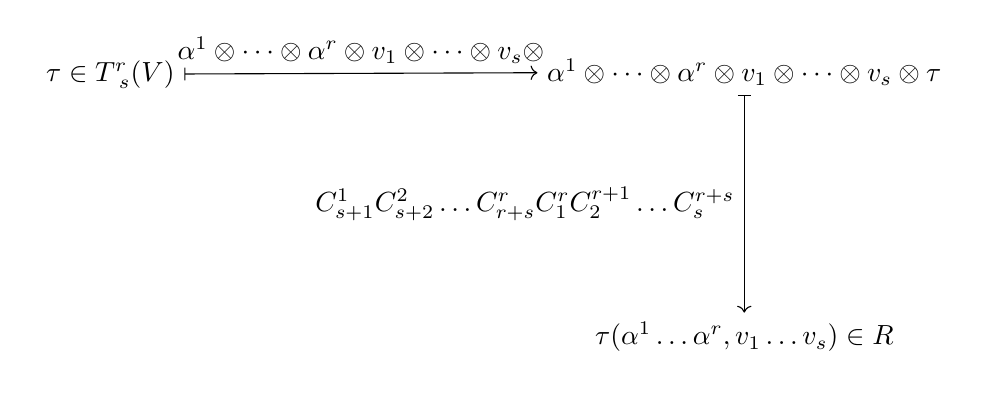
\begin{tikzpicture}
  \matrix (m) [matrix of math nodes, row sep=7.8em, column sep=12.8em, minimum width=5.2em]
  {
  \tau \in T^r_{\,\,s}(V)  &  \alpha^1 \otimes \dots \otimes \alpha^r \otimes v_1\otimes \dots \otimes v_s \otimes \tau  \\ 
& \tau(\alpha^1\dots \alpha^r,v_1\dots v_s)  \in R \\ 
};
  \path[|->]
  (m-1-1) edge node [above] {$ \alpha^1\otimes \dots \otimes \alpha^r \otimes v_1 \otimes \dots \otimes v_s \otimes $} (m-1-2)
  (m-1-2) edge node [left] {$C^1_{ s+1} C^2_{s+2}\dots C^r_{r+s} C^r_1 C_2^{r+1}\dots C_s^{r+s} $} (m-2-2)
  ;
\end{tikzpicture}  
\]
where I've tried to express the right-$R$-module, "right action" on $\alpha^1 \otimes \dots \otimes \alpha^r \otimes v_1\otimes \dots \otimes v_s \in V^*\otimes \dots \otimes V$.  


Conlon (2008) \cite{Conl2008}

\subsection{Metric}

\subsubsection{Induced Metric}

cf. 7.1.2. Induced metric, Nakahara (2003) \cite{Naka2003}. Let $M$ be $m$-dim. submanifold of $n$-dim. Riemannian manifold $N$ with metric $g_N$. \\
If $f:M \to N$ embedding which induced the submanifold structure of $M$. (Sec. 5.2 of Nakahara (2003) \cite{Naka2003}). \\
(Recall, smooth $f: M \to N$, $\text{dim}M \leq N$, $f$ immersion if $f_* : T_pM \to T_{f(p)}N$ injection, so rank $f_* = \text{dim}M$. $f$ embedding if $f$ immersion and $f$ injection. Also $f(M)$ submanifold of $N$).

\begin{proposition}
pullback $f^*$ induced a natural metric $g_M = f^* g_N$ on $M$ is given by
\begin{equation}
	g_{M\mu nu} (x) = g_{N \alpha \beta} \frac{\partial f^{\alpha}}{\partial x^{\mu}}\frac{\partial f^{\alpha} }{ \partial x^{\nu}}
\end{equation}
\end{proposition}

Recall that
\[
\begin{gathered}
\begin{aligned}
	& f^* : T^*_{f(p)}N \to T_p^* M \\
	& \omega \in T^*_{f(p)}N \\
	& V \in T_p M
\end{aligned} \quad \quad \, 
\begin{gathered}
\langle f^* \omega, V \rangle = \langle \omega, f_* V \rangle \\
\text{ and } \\
f_*V[g] = V[gf], \, g\in \mathcal{F}(N)
\end{gathered}
\end{gathered}
\]

Using our notation, consider \\
\[
\begin{aligned}
	& (U, \varphi), \, U\subset M, \, \varphi : U \subset M \to \mathbb{R}^m \\
	& (V, \psi), \, V \subset N, \, \psi : V \subset N \to \mathbb{R}^n
\end{aligned}
\]
Colloquially, say $y^j = y^j(x)$, but actually $y^j = \psi \circ f\circ \varphi^{-1}$, so that
\[
f_*(X) = Y, \text{ where } X= X^i \frac{ \partial }{ \partial x^i }, \, Y = Y^j \frac{\partial }{ \partial y^j} = X^i \frac{ \partial y^j}{\partial x^i } \frac{ \partial }{ \partial y^j}
\]

We also observe that 
\[
f_* V[g] = V[g\circ f] = V^i \frac{ \partial }{ \partial x^i} (g\circ f) = V^i \frac{ \partial g}{ \partial y^i} \frac{ \partial f^j}{ \partial x^i } = V^i \frac{ \partial f^j}{ \partial x^i } \frac{ \partial g}{ \partial y^j}
\]
where notation-wise, $X\equiv V$, $y\equiv f$ with respect to ours and Nakahara's notation. \\

Now $g_N : T_{f(p)}N \otimes T_{f(p)} N \to \mathbb{R}$, then if we just input one vector into $g_N$, it becomes a covector $g_N(U, \,) \in T^*_{f(p)} N$.

So then
\[
\begin{gathered}
	\langle f^* g_N(U, \, ) , V \rangle = \langle g_N(U, \, ) , f_* V\rangle = \langle g_N(U, \, ) , V^i \frac{ \partial f^j}{ \partial x^i} \frac{ \partial }{ \partial y^j} \rangle = \langle g_N(U, \, ) , V^i \frac{ \partial }{ \partial y^j} \rangle \frac{ \partial f^j }{ \partial x^i} \\
g_N(U, V^i \frac{ \partial }{ \partial y^i } ) \frac{ \partial f^j}{\partial x^i} = g_N(U^k \frac{ \partial }{ \partial y^k}, V^i \frac{ \partial }{ \partial y^j} ) \frac{ \partial f^j}{\partial x^i} = (g_N)_{aj} V^i \frac{\partial f^j}{\partial x^i} 
\end{gathered}
\]
where we let $U^k = \delta^{ak}$ in the last step.

Let $V =\delta^{bi} \frac{\partial }{ \partial x^i} $, so $(g_N)_{aj} \frac{ \partial f^j}{\partial x^b} = \langle f^* g_N \left(\frac{\partial }{ \partial y^a} , \, \right), \frac{\partial }{ \partial x^b} \rangle $. 

By symmetry,
\begin{equation}
\boxed{ (g_M)_{ab} = (g_N)_{ij} \frac{ \partial f^i}{ \partial x^a } \frac{ \partial f^j}{\partial x^b} }
\end{equation}
where $f:M \to N$.

\problemhead{8, pp. 28, Wald (1984) \cite{Wald1984}}

\begin{enumerate}
	\item[(a)] The metric of flat, 3-dim. Euclidean space is
	\[
	ds^2 = dx^2 + dy^2 + dz^2
	\]
	Show that the metric components $g_{\mu \nu}$ in spherical polar coordinates $r, \theta, \phi$ defined by
	\[
	\begin{gathered}
		r= (x^2 + y^2 + z^2)^{1/2} \\
		\cos{\theta}  =  z/r \\
		\tan{\phi} = y/x
	\end{gathered}
	\]
	is given by
	\[
	ds^2 = dr^2 + r^2 d\theta^2 + r^2 \sin^2{\theta} d\phi^2
	\]
	\item[(b)] The spacetime metric of special relativity is 
	\[
	ds^2 = -dt^2 + dx^2 + dy^2 + dz^2
	\]
	Find the components, $g_{\mu \nu}$ and $g^{\mu \nu}$, of the metric and inverse metric in "rotating coordinates," defined by
	\[
	\begin{aligned}
		& t' = t \\
		& x' = (x^2 + y^2)^{1/2} \cos{(\phi - \omega t)} \\
		& y' = (x^2 + y^2)^{1/2} \sin{(\phi - \omega t)} \\
		& z' =z
	\end{aligned}
	\]
	where $\tan{\phi} = y/x$.
\end{enumerate}

\solutionhead{8, pp. 28, Wald (1984) \cite{Wald1984}}
\begin{enumerate}
	\item[(a)] Consider $(r,\theta, \varphi) \to (x,y,z)$ s.t. 
	\[
	\begin{gathered}
	\begin{aligned}
		& x = rs{\theta} c{\varphi} \\
		& y = rs{\theta} s{\varphi} \\
		& z = rc{\theta}
	\end{aligned}
\text{ so consider } \left| \begin{matrix} s{\theta} c{\varphi} & rc{\theta} c{\varphi} & - rs{\theta} s{\varphi} \\
	s{\theta} s{\varphi} & rc{\theta} s{\varphi} & rs{\theta} c{\varphi} \\
	c{\theta} & -rs{\theta} & 0 \end{matrix} \right|
	\end{gathered}
	\]
	Since $(g_N)_{ij} = \delta_{ij}$ in our case,
	\[
	\begin{aligned}
		& (g_M)_{rr} = 1 \\
		& (g_M)_{\theta \theta} = r^2 \\
		& (g_M)_{\varphi \varphi} = r^2 \sin^2{\theta}
	\end{aligned}
	\]
	By summing terms across columns, $(g_M)_{ab} =0$ if $a\neq b$ and $(g_M)_{aa}$ obtained by squaring and summing terms across a single column.

	Thus, some physicists write as a (sometimes confusing) shorthand for the metric tensor
	\[
	g_M = dr \otimes dr + r^2 d\theta \otimes d\theta + r^2 \sin^2{\theta} d\varphi \otimes d\varphi
	\]
	to be
	\[
	ds^2 = dr^2 + r^2 d\theta^2 + r^2 \sin^2{\theta} d\phi^2	
	\]
	\item[(b)] Consider $(t', x', y', z') \to (t, x, y, z)$. Let $\rho = (x^2 + y^2)^{1/2}$. Consider the Jacobian:
	\[
	\left| \begin{matrix} 1 & & & \\ 
		\omega \rho s(\phi - \omega t) & \frac{x}{\rho} c(\phi - \omega t) &  \frac{y}{\rho} c(\phi - \omega t) & \\
		 -\omega \rho  c(\phi - \omega t) &  \frac{x}{\rho} s(\phi - \omega t) &  \frac{y}{\rho} s(\phi - \omega t) & \\
		 0 & & 1 \end{matrix} \right|
	\]

The terms with the same components, e.g. $g_{t't'}, \, g_{x'x'}, \dots$ are $(-1 + \omega^2 \rho^2), \, \frac{x^2}{\rho^2} , \, \frac{y^2}{\rho^2}, \, 1$, and the cross terms are $\frac{xy}{\rho^2} dx \otimes dy$.
\end{enumerate}


\part{Lie Groups, Lie Algebra}

\section{Lie Groups}

\begin{description}
	\item Lie Groups 
	\item Groups
	\item Ring
	\item group algebra
	\item Group Ring
	\item Representation Theory
	\item Modules
	\item $kG$-modules
\end{description}

From Sec. 8.1 ``Noncommutative Rings'' of Rotman (2010) \cite{JRotman2010}:

\begin{definition}
	ring $R$ - additive abelian group equipped with multiplication $\begin{aligned} & \quad \\ 
	& R \times R \to R \\
	& (a,b) \mapsto ab \end{aligned}$ s.t. $\forall \, a ,b \in R$
	
	\begin{enumerate}
		\item[(i)] $a(bc) = (ab)c$ 
		\item[(ii)] $a(b+c) = ab+ ac$, $(b+c)a = ba + ca$ 
		\item[(iii)] $\exists \, 1 \in R$ s.t. $\forall \, a \in R$, $1a = a = a1$
	\end{enumerate}
\end{definition}

Example 8.1\cite{JRotman2010}
\begin{enumerate}
	\item[(ii)] group algebra $kG$, $k$ commutative ring, $G$ group, ``its additive abelian group is free $k$-module having basis labeled by elements of $G$, \\
	i.e. $\forall \, a \in kG$, $a = \sum_{g\in G} a_g g$, $a_g \in k$, \, $\forall \, g \in G$, $a_g \neq 0$ for only finitely many $g\in G$.  
	
	define (ring) multiplication $\begin{aligned} & \quad \\ 
	& kG \times kG \to kG \\
	& ab = ab \end{aligned}$ \, $\forall \, a,b \in kG$, $\begin{aligned} & \quad \\ 
	& a = \sum_{g\in G} a_g g \\
	& b = \sum_{h \in G} b_h g \end{aligned}$ to be 
	\[
	\left( \sum_{g \in G} a_g g \right) \left( \sum_{h \in G} b_h h \right) = \sum_{ z\in G} \left( \sum_{ gh = z} a_g b_h \right)z
	\]
	
\end{enumerate}

\begin{definition}
	Given $R$ ring, left $R$-module is (additive) abelian group $M$ equipped with \\
	scalar multiplication $\begin{aligned} & \quad \\
	& R \times M \to M \\
	& (r,m) \mapsto rm \end{aligned}$ s.t. $\forall \, m , m' \in M$, $\forall \, r, r' , 1 \in R$
	\begin{enumerate}
		\item[(i)] $r (m+m') = rm + rm' $ 
		\item[(ii)] $(r+r')m = rm + r'm $ 
		\item[(iii)] $(rr')m = r(r'm)$
		\item[(iv)] $1m = m$
	\end{enumerate}
\end{definition}

EY : 20150922 Example : for $kG$-module $V^{\sigma}$, for $r \in kG$, so $r= \sum_{g\in G} a_g g$ 
\[
\begin{aligned} & R \times M \to M \\
& (r,m) \mapsto rm \end{aligned} \Longrightarrow \begin{aligned} & kG \times V \to V \\
& (r,v) \mapsto tv \end{aligned}
\]
For some representation $\sigma : G \to GL(V)$, 
\[
rv = \sum_{g \in G} a_g g \cdot v =\sum_{g\in G} a_g \sigma_g(v)
\]
So a $kG$-module needs to be associated with some chosen representation.  

Note for $V$ as an additive abelian group, $\forall \, u,v,w \in V$, 
\[
\begin{aligned}
& v+w = w+v, \, (u+v) + w = u+(v+w) \\ 
& v+0 = v \quad \, \forall \, v \in V \text{ for } 0 \in V \\ 
& v+ (-v) =0 \quad \, \forall \, v \in V
\end{aligned}
\]
So a vector space can be an additive abelian group.  

Note that 
\[
\begin{gathered}
r(v+w) = \left( \sum_{g\in G} a_g g \right)(v+w) = \left( \sum_{g \in G} a_g \sigma_g \right)(v+w) = \sum_{g\in G} a_g \sigma_g(v) + \sum_{g\in G} a_g \sigma_g(w) = rv + rw \\ 
(r+r')v = \left( \sum_{g\in G} a_g g + b_g g \right) v =\sum_{g\in G} (a_g \sigma_g + b_g \sigma_g ) v = \sum_{g \in G}a_g \sigma_g(v) + \sum_{g\in G}b_g \sigma_g(v) = rv + r'v 
\end{gathered}
\]
\[
\begin{gathered}
(rr')v = \left( \sum_{g\in G} a_g g \sum_{h \in G} b_h h \right)v = \left( \sum_{z\in G} \sum_{gh = z} a_g b_h z \right) v = \sum_{z\in G} \sum_{gh \in z} a_g b_h \sigma_z(v) = \sum_{g\in G} \sum_{h \in G} a_g b_h \sigma_g \sigma_h (v)
\end{gathered}
\]
since $\sigma(gh) = \sigma(g) \sigma(h) = \sigma_g \sigma_h = \sigma_{gh}$ ($\sigma$ homomorphism)

$1v = \sigma(1) v = 1v = v$



From Sec. 8.3 ``Semisimple Ring'' of Rotman (2010) \cite{JRotman2010}:

\begin{definition}
	$k$-representation of group $G$ is homomorphism
	\[
	\sigma : G \to GL(V)
	\]
	where $V$ is vector field over field $k$
\end{definition}

\begin{proposition}[8.37 Rotman (2010)\cite{JRotman2010}]\label{Prop:Rotman8.37}
	$\forall \, k$-representation $\sigma : G \to GL(V)$ equips $V$ with structure of left $kG$-module, denote module by $V^{\sigma}$.  \\
	Conversely, $\forall \, $ left $kG$-module $V$ determines $k$-representation $\sigma:G \to GL(V)$
\end{proposition}

\begin{proof}
	Given $\begin{aligned} & \quad \\
	\sigma & :G \to GL(V) \\
	\sigma_g =: \sigma(g) & : V \to V \end{aligned}$, 
	
	define 
	\[
	\begin{aligned}
	kG \times V & \to V \\ 
	\left( \sum_{g\in G} a_g g \right) v & = \sum_{g\in G} a_g \sigma_g(v) 
	\end{aligned}
	\]
	
	Let $\begin{aligned} & \quad \\ 
	& v,w \in V \\
	& r,r',1 \in kG \\
	& r = \sum_{g\in G} a_g g \end{aligned}$
	
	\[
	\begin{gathered}
	r(v+w) = \left( \sum_{g\in G} a_g g \right)(v+w) = \left( \sum_{g \in G} a_g \sigma_g \right)(v+w) = \sum_{g\in G} a_g \sigma_g(v) + \sum_{g\in G} a_g \sigma_g(w) = rv + rw \\ 
	(r+r')v = \left( \sum_{g\in G} a_g g + b_g g \right) v =\sum_{g\in G} (a_g \sigma_g + b_g \sigma_g ) v = \sum_{g \in G}a_g \sigma_g(v) + \sum_{g\in G}b_g \sigma_g(v) = rv + r'v 
	\end{gathered}
	\]
	\[
	\begin{gathered}
	(rr')v = \left( \sum_{g\in G} a_g g \sum_{h \in G} b_h h \right)v = \left( \sum_{z\in G} \sum_{gh = z} a_g b_h z \right) v = \sum_{z\in G} \sum_{gh \in z} a_g b_h \sigma_z(v) = \sum_{g\in G} \sum_{h \in G} a_g b_h \sigma_g \sigma_h (v)
	\end{gathered}
	\]
	since $\sigma(gh) = \sigma(g) \sigma(h) = \sigma_g \sigma_h = \sigma_{gh}$ ($\sigma$ homomorphism)
	
	$1v = \sigma(1) v = 1v = v$
	
	Conversely, assume $V$ left $kG$-module.
	
	If $g \in G$, then $v\mapsto gv$ defines $T_g:V \to V$.  $T_g$ nonsingular since $\exists \, T_g^{-1} = T_{g^{-1}}$
	
	Define $\begin{aligned} & \quad \\
	& \sigma : G \to GL(V) \\
	& \sigma: g \mapsto T_g \end{aligned}$ \quad \\
	
	$\sigma$ $k$-representation
	\[
	\begin{aligned}
	& \sigma(gh) = T_{gh} = T_g T_h = \sigma(g)\sigma(h) \\
	& \sigma(gh)(v) = T_{gh}v = ghv = T_gT_h v = \sigma(g)\sigma(h)v \quad \, \forall \, v \in V
	\end{aligned}
	\]
	
\end{proof}

\begin{proposition}
	Let group $G$, let $\sigma, \tau: G \to GL(V)$ be $k$-representations, field $k$.  \\
	If $V^{\sigma}, V^{\tau}$ corresponding $kG$-modules in Prop. \ref{Prop:Rotman8.37} (Prop. 8.37 in Rotman (2010) \cite{JRotman2010}), then \\
	$V^{\sigma} \simeq V^{\tau}$ as $kG$-modules iff $\exists \, $ nonsingular $\varphi :V \to V$ s.t. 
	\[
	\varphi \tau(g) = \sigma(g) \varphi \quad \, \forall \, g \in G
	\]
	
\end{proposition}

\begin{proof}
	If $\varphi : V^{\tau} \to V^{\sigma}$ $kG$-isomorphism, then $\varphi : V \to V$ isomorphism s.t.
	\[
	\varphi( \sum a_g g v ) = (\sum a_g g)\varphi(v) \quad \, \forall \, v \in V, \, \forall \, g \in G
	\]
	in $V^{\tau}$, $\begin{aligned} & \quad \\
	& kG \times V \to V \\
	& gv = \tau(g)(v) \end{aligned}$ \quad \quad \, in $V^{\sigma}$, $\begin{aligned} & \quad \\
	& kG \times V \to V \\
	& gv = \sigma(g)(v) \end{aligned}$ scalar multiplication
	
	\[
	\begin{gathered}
	\Longrightarrow \forall \, g \in G, v\in V, \quad \, \varphi(\tau(g)(v)) = \sigma(g)(\varphi(v))
	\end{gathered}
	\]
	I think 
	\[
	\varphi(gv) = \varphi(\tau(g)(v)) = g\varphi(v) = \sigma(g)\varphi(v)
	\]
	\[
	\Longrightarrow \varphi \tau(g) = \sigma(g) \varphi \quad \, \forall \, g \in G
	\]
	Conversely, if $\exists \, $ nonsingular $\varphi : V \to V$ s.t. $\begin{aligned} & \quad \\ 
	& \varphi \tau (g) = \sigma(g) \varphi \quad \, \forall \, g \in G \\
	& \varphi \tau(g) v = \varphi(\tau(g)v) = \sigma(g)\varphi(v) \quad \, \forall \, g \in G, \, \forall \, v \in V \end{aligned}$
	
	Consider scalar multiplication
	\[
	\begin{gathered}
	kG \times V \to V \\ 
	\sum_{g\in G} a_g g(v) = \sum_{g\in G} a_g \tau_g(v)
	\end{gathered}
	\]
	\[
	\varphi \left( \sum_{g\in G} a_g \tau_g(v) \right) = \varphi \left( \sum_{g\in G} a_g \tau(g) v\right) = \sum_{g\in G} a_g \sigma(g) \sigma(g)\varphi(v) = \left( \sum_{g\in G} a_g g \right) \varphi(v)
	\]
	
\end{proof}

Admittedly, after this exposition from Rotman (2010) \cite{JRotman2010}, I still didn't understand how $kG$-modules relate to representation theory and group rings.  I turned to Baker (2011) \cite{ABaker2011}, which we'll do right now.  Note that I found a lot of links to online resources on representation theory from Khovanov's webpage \url{http://www.math.columbia.edu/~khovanov/resource/}.  

Note, 
\begin{definition}
	vector subspace $W \subseteq V$ is called a \\
	$G$-submodule, $G$-subspace, EY : 20150922 ``invariant'' subspace? \\
	if $\forall \, g \in G$, for representation $\rho : G \to GL_k(V)$, $\rho_g(w) \in W$, \, $\forall \, w \in W$, $\forall \, g \in G$ i.e. closed under ``action of elements of $G$'' with \\
	$\rho_g =: \rho (g): V \to V$
\end{definition}

Given basis $\mathbf{v} = \lbrace v_1 \dots v_n \rbrace$ for $V$, $\text{dim}_kV = n$, $\forall \, g \in G$, 
\[
\rho_g v_j = \rho(g) v_j = r_{kj}(g) v_k
\]
for, indeed, 
\[
\rho_g x^j v_j = \rho(g) x^j v_j = x^j\rho(g) v_j = x^j r_{kj}(g) v_k = r_{kj} x^j v_k
\]
so that 
\[
\begin{aligned}
& \rho : G \to GL_k(V) \\ 
& \rho(g) = [r_{ij}(g)]
\end{aligned}
\]

Example 2.1 (Baker (2011) \cite{ABaker2011}): Let $\rho :G \to GL_k(V)$ where $\text{dim}_kV=1$
\[
\begin{gathered}
\forall \, v \in V, \, v\neq 0 , \forall \, g \in G, \, \lambda_g \in k \text{ s.t. } g \cdot v = \rho_g(v) = \lambda_g v \\ 
\rho(hg) v = \rho_h \rho_g v = \lambda_{hg} v = \lambda_h \lambda_g v \Longrightarrow \lambda_{hg} = \lambda_h \lambda_g
\end{gathered}
\]
$\Longrightarrow \exists \, $ homomorphism $\begin{aligned} & \quad \\
& \Lambda : G \to k^{\times } \\
& \Lambda(g) = \lambda_g \end{aligned}$


From Sec. 2.2 ``$G$-homomorphisms and irreducible representations'' of Baker (2011) \cite{ABaker2011}, suppose $\begin{aligned} & \rho : G \to GL_k(V) \\
& \sigma : G \to GL_k(W) \end{aligned}$ are 2 representations

Many names for the same thing: $G$-equivalent, $G$-linear, $G$-homomorphism, EY : 20150922 $kG$-isomorphic?

If $\forall \, g \in G$, 

\begin{tikzpicture}
\matrix (m) [matrix of math nodes, row sep=3.8em, column sep=4.8em, minimum width=2.2em]
{
	V & V \\
	V & V \\
};
\path[->]
(m-1-1) edge node [above] {$\varphi$} (m-1-2)
edge node [left] {$\tau_g$} (m-2-1)
(m-1-2) edge node [auto]  {$\sigma_g$} (m-2-2)
(m-2-1) edge node [auto]  {$\varphi$} (m-2-2)
;
\end{tikzpicture}  $\Longleftrightarrow  V^{\tau} \overset{\varphi}{\simeq} V^{\sigma}$

Indeed, define 
\[
\begin{aligned}
& \varphi: V^{\tau} \to V^{\sigma} \\ 
& \varphi(v+w) = \varphi(v) + \varphi(w) \\ 
& \varphi(rv) = \varphi( \sum_{g\in G} a_g g \cdot v) = \varphi( \sum_{g \in G} a_g \tau_g(v) ) = \sum_{ g\in G} a_g \varphi(\tau_g(v)) = \sum_{g\in G} a_g \sigma_g \cdot \varphi(v) = r\varphi(v)
\end{aligned}
\]
EY : 20150922 So $\varphi$ is a $kG$-isomorphism between left $kG$ modules $V^{\tau}$ and $V^{\sigma}$ if it's bijective and is ``linear'' in ``scalars'' $r\in kG$, i.e. $\varphi(rv) = r\varphi(v)$.  

Define action of $G$ on $\text{Hom}_k(V,W)$ ($\text{Hom}_k(V,W)$ is the vector space of $k$-linear transformations $V\to W$) \\
$\forall \, f \in \text{Hom}_k(V,W)$, $\begin{aligned} & \quad \\
& f : V \to W \\
& f(v) \in W \end{aligned}$ \quad \, 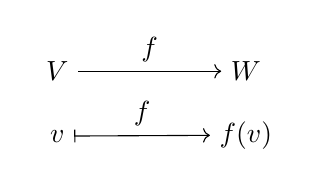
\begin{tikzpicture}
\matrix (m) [matrix of math nodes, row sep=0.8em, column sep=4.8em, minimum width=0.2em]
{
	V & W \\
	v & f(v) \\
};
\path[->]
(m-1-1) edge node [above] {$f$} (m-1-2)
;
\path[|->]
(m-2-1) edge node [auto] {$f$} (m-2-2)
;
\end{tikzpicture}

Consider

\[
\begin{aligned}
& G \times \text{Hom}_k(V,W) \to \text{Hom}_k(V,W) \\ 
& (g\cdot f) \mapsto (\sigma_g f) \circ \rho_{g^{-1}} \text{ i.e. } (g\cdot f)(v) = \sigma_gf(\rho_{g^{-1}}v) \quad \, (f\in \text{Hom}_k(V,W))
\end{aligned}
\]
Let $g,h \in G$, 
\[
(gh \cdot f)(v) = g\cdot \sigma_h f(\rho_{h^{-1}}v) = \sigma_g\sigma_h f\rho_{h^{-1}} \rho_{g^{-1}}(v) = (\sigma_{gh} f \rho_{(gh)^{-1}} )(v)
\]

Thus,  $\begin{aligned} & \quad \\
& G \times \text{Hom}_k(V,W) \to \text{Hom}_k(V,W) \\ 
& (g\cdot f) \mapsto (\sigma_g f)\circ \rho_{g^{-1}} \end{aligned}$ is thus another $G$-representation of $G$.  

For $k$-representation $\rho$, if the only $G$-subspaces of $V$ are $\lbrace 0 \rbrace$, $V$, $\rho$ \textbf{irreducible} or \textbf{simple}.  
\[
\begin{aligned}
& \rho_g(\lbrace 0 \rbrace) = \lbrace 0 \rbrace \\ 
&  \rho_g(V) = V
\end{aligned}
\]


given subrepresentation $W \subseteq V$, $V/W$ admits linear action of $G$, $\overline{\rho}_W : G \to GL_k(V/W)$ quotient representation 
\[
\overline{\rho}_W(g)(v+W) = \rho(g)(v) + W
\]
if $v'-v \in W$
\[
\rho(g)(v') + W = \rho(g)(v+(v'-v))+W = (\rho(g)(v) + \rho(g)(v'-v) ) + W = \rho(g)(v) + W
\]
\begin{proposition}[2.7 Baker (2011)\cite{ABaker2011}] \label{Prop:Baker2.7}
	if $f:V \to W$ $G$-homomorphism, then
	\begin{enumerate}
		\item[(a)] $\text{ker}{f}$ is $G$-subspace of $V$ 
		\item[(b)] $\text{im}{f}$ is $G$-subspace of $W$
	\end{enumerate}
\end{proposition}

\begin{proof}
	Recall 
	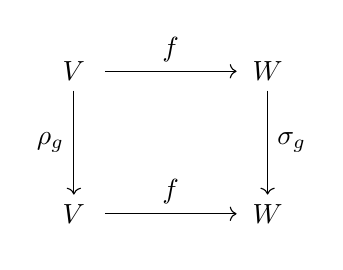
\begin{tikzpicture}
	\matrix (m) [matrix of math nodes, row sep=3.8em, column sep=4.8em, minimum width=2.2em]
	{
		V & W \\
		V & W \\
	};
	\path[->]
	(m-1-1) edge node [above] {$f$} (m-1-2)
	edge node [left] {$\rho_g$} (m-2-1)
	(m-1-2) edge node [auto]  {$\sigma_g$} (m-2-2)
	(m-2-1) edge node [auto]  {$f$} (m-2-2)
	;
	\end{tikzpicture}
	
	\begin{enumerate}
		\item[(a)] Let $v\in \text{ker}{f}$.  Then $\forall \, g \in G$, 
		\[
		f(\rho_g v) = \sigma_g f(v) = 0 
		\]
		so $\rho_g v \in \text{ker}{f}$, $\forall \, g \in G$.  So $\text{ker}{f}$ is $G$-subspace of $V$
		\item[(b)] Let $w\in \text{im}{f}$.  So $w = f(u)$ for some $u \in V$ 
		\[
		\sigma_g w = \sigma_g f(u) = f(\rho_gu) \in \text{im}f
		\]
		So $\text{im}{f}$ is $G$-subspace of $W$
	\end{enumerate}
\end{proof}

\begin{theorem}[Schur's Lemma]
	Let $\begin{aligned} & \quad \\
	& \rho : G \to GL_{\mathbb{C}}(V) \\
	& \sigma : G \to GL_{\mathbb{C}}(W) \end{aligned}$ be irreducible representations of $G$ over field $k= \mathbb{C}$; let $f:V \to W$ be $G$-linear map.  
	
	\begin{enumerate}
		\item[(a)] if $f\neq 0$, $f$ isomorphism.  True $\forall \, k$ field, not just $\mathbb{C}$
		\item[(b)] if $V=W$, $\rho = \sigma$, then for some $\lambda \in \mathbb{C}$, $f$ given by $f(v) = \lambda v$ ($v\in V$) (true for algebraically closed fields)
	\end{enumerate}
\end{theorem}

\begin{proof}
	\begin{enumerate}
		\item[(a)] By Prop. \ref{Prop:Baker2.7}, $\text{ker}f \subseteq V$, $\text{im}f \subseteq W$ are $G$-subspaces.  \\
		For $\rho$, only $G$-subspaces are $0$ or $V$, so if $\text{ker}f = V$, $f=0$.  If $\text{ker}f = 0$, $f$ injective.  \\
		For $\sigma$, only $G$-subspaces are $0$ or $V$, so $\text{im}f =0 $, $f=0$.  If $\text{im}f =V$, $f$ surjective.  
		
		$\Longrightarrow f$ isomorphism.  
		\item[(b)] Let $\lambda \in \mathbb{C}$ be an eigenvalue of $f$, $f(v_0) = \lambda v_0$ eigenvector, $v_0 \neq 0$.  
		
		Let linear $f_{\lambda} : V \to V$ s.t. 
		\[
		f_{\lambda}(v) = f(v) - \lambda v \quad \, (v\in V)
		\]
		$\forall \, g \in G$
		\[
		\rho_g f_{\lambda}(v) = \rho_gf(v) - \rho_g \lambda v = f(\rho_g v) - \lambda \rho_g v= f_{\lambda}(\rho_g v)
		\]
		So $f_{\lambda}$ is $G$-linear, for 
		
		\begin{tikzpicture}
		\matrix (m) [matrix of math nodes, row sep=3.8em, column sep=4.8em, minimum width=2.2em]
		{
			V & V \\
			V & V \\
		};
		\path[->]
		(m-1-1) edge node [above] {$f$} (m-1-2)
		edge node [left] {$\rho_g$} (m-2-1)
		(m-1-2) edge node [auto]  {$\rho_g$} (m-2-2)
		(m-2-1) edge node [auto]  {$f$} (m-2-2)
		;
		\end{tikzpicture}
		
		Since $f_{\lambda}(v_0) =0$, by Prop. \ref{Prop:Baker2.7}, $\text{ker}f_{\lambda} = V$, (for $\text{ker}f_{\lambda}\neq 0$ and so $\text{ker}f_{\lambda}=V$)
		
		By rank-nullity theorem, $\text{dim}V = \text{dim}\text{ker}f_{\lambda} + \text{dim}\text{im}f_{\lambda}$.  
		
		So $\text{im}f_{\lambda}=0$, and so $f_{\lambda}(v)=0$ ($\forall \, v \in V$) $\Longrightarrow f(v) = \lambda v$
	\end{enumerate}
\end{proof}

Schur's lemma, at least the first part, implies that the left $kG$-modules associated with representations $\rho, \sigma$ are $kG$-isomorphic, i.e.

\[
\begin{gathered}
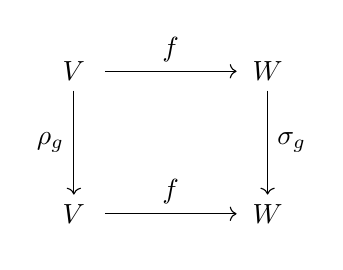
\begin{tikzpicture}
\matrix (m) [matrix of math nodes, row sep=3.8em, column sep=4.8em, minimum width=2.2em]
{
	V & W \\
	V & W \\
};
\path[->]
(m-1-1) edge node [above] {$f$} (m-1-2)
edge node [left] {$\rho_g$} (m-2-1)
(m-1-2) edge node [auto]  {$\sigma_g$} (m-2-2)
(m-2-1) edge node [auto]  {$f$} (m-2-2)
;
\end{tikzpicture}  \Longleftrightarrow  V^{\rho} \overset{f}{\simeq} V^{\sigma}
\end{gathered}
\]

with $f$ being an isomorphism between $V^{\rho}$ and $V^{\sigma}$ s.t. 
\[
\begin{gathered}
f(v+w) = f(v) + f(w) \quad \, \forall \, v,w \in (V^{\sigma},+) \\ 
f(rv) = rf(v) \quad \, \forall \, r  = \sum_{g \in G} a_g g \in kG
\end{gathered}
\]

Kosmann-Schwarzbach's \textbf{Groups and Symmetries}\cite{YKosmann-Schwarzbach2010} is a very lucid text that's mathematically rigorous enough and practical for physicists.  It's really good and very clear.  Let's follow its development for $SU(2), SO(3), SL(2,\mathbb{C})$ and corresponding Lie algebras $\mathfrak{su}(2)$, $\mathfrak{so}(3)$, $\mathfrak{sl}(2,\mathbb{C})$.  

From Chapter 2 ``Representations of Finite Groups'' of Kosmann-Schwarzbach (2010) \cite{YKosmann-Schwarzbach2010}

\begin{definition}[2.1 Kosmann-Schwarzbach (2010)\cite{YKosmann-Schwarzbach2010}] \label{Def:2.1scalarproductG}
	On $L^2(G)$, scalar product defined by 
	\[
	\langle f_1 | f_2 \rangle = \frac{1}{|G|} \sum_{g\in G} \overline{f_1(g)} f_2(g)
	\]
	$f_1,f_2 \in \mathcal{F}(G) \equiv \mathbb{C}[G]$ vector space of functions on $G$ taking values on $\mathbb{C}$
\end{definition}

\begin{definition}[2.3 Kosmann-Schwarzbach (2010)\cite{YKosmann-Schwarzbach2010}]
	Let $(E,\rho)$ be representation of $G$ \\
	character of $\begin{aligned} & \quad \\ 
	\rho \equiv \chi_{\rho} & : G \to \mathbb{C} \\
	\chi_{\rho}(g) & = \text{tr}( \rho(g)) = \sum_{i=1}^n (\rho(g))_{ii} \end{aligned}$ 
	
	Note: equivalent representations have same character \\
	each conjugacy class of $G$, function $\chi_p$ is constant
\end{definition}

Looking at Def. \ref{Def:2.1scalarproductG}
\[
\langle \chi_{\rho_1} | \chi_{\rho_2} \rangle = \frac{1}{|G| } \sum_{g\in G} \chi_{\rho_1}(g^{-1}) \chi_{\rho_2(g)}
\]
since $\overline{\chi_{\rho_1(g)}} = \chi_{\rho_1}(g^{-1})$ by unitarity of representation with respect to scalar product $\langle \, , \, \rangle$

\begin{proposition}[2.7 Kosmann-Schwarzbach (2010)\cite{YKosmann-Schwarzbach2010}]
	Let $\begin{aligned} & \quad \\ 
	& (E_1, \rho_1) \\
	& (E_2, \rho_2) \end{aligned}$ be representations of $G$, let linear $u: E_1 \to E_2$.  
	
	Then $\exists \, $ linear $T_u$ s.t. 
	
	\begin{equation}\label{Eq:T_ucharacters}
	\begin{aligned} & \quad \\
	& T_u : E_1 \to E_2 \\
	& T_u = \frac{1}{|G|} \sum_{g\in G} \rho_2(g)u\rho_1(g)^{-1} \end{aligned}
	\end{equation}
	
	so that $\rho_2(g) T_u = T_u\rho_1(g) \quad \, \forall \, g \in G$
\end{proposition}

\begin{proof}
	\[
	\rho_2(g) T_u = \frac{1}{|G|} \sum_{ h \in G } \rho_2(gh) u \rho_1(h^{-1}) = \frac{1}{|G|} \sum_{ k \in G} \rho_2(k) u \rho_1(k^{-1}g) = T_u \rho_1(g)
	\]
\end{proof}

Thus, diagrammatically, we have that 
\[
\begin{tikzpicture}
\matrix (m) [matrix of math nodes, row sep=3.8em, column sep=4.8em, minimum width=2.2em]
{
	E_1 & E_2 \\
};
\path[->]
(m-1-1) edge node [above] {$u$} (m-1-2)
;
\end{tikzpicture} \Longrightarrow  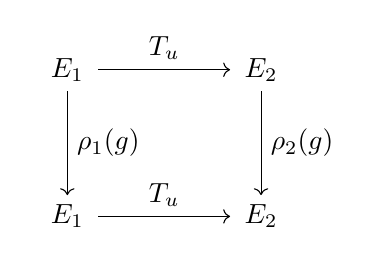
\begin{tikzpicture}
\matrix (m) [matrix of math nodes, row sep=3.8em, column sep=4.8em, minimum width=2.2em]
{
	E_1 & E_2 \\
	E_1 & E_2 \\
};
\path[->]
(m-1-1) edge node [above] {$T_u$} (m-1-2)
edge node [auto] {$\rho_1(g)$} (m-2-1)
(m-1-2) edge node [auto]  {$\rho_2(g)$} (m-2-2)
(m-2-1) edge node [auto]  {$T_u$} (m-2-2)        
;
\end{tikzpicture}
\]

From Definition	1.12 of	Kosmann-Schwarzbach \cite{YKosmann-Schwarzbach2010}, ``representations $\rho_1$ and $\rho_2$ are called \textbf{equivalent} if there is a bijective intertwining operator for $\rho_1$ and $\rho_2$.''  So I will interpret this as if an intertwining operator is not bijective, then the representations $\rho_1$, $\rho_2$ are not equivalent.  

\begin{proposition}[2.8 Kosmann-Schwarzbach (2010)\cite{YKosmann-Schwarzbach2010}]
	Let $\begin{aligned}
	& \quad \\
	& (E_1,\rho_1) \\
	& (E_2,\rho_2) \end{aligned}$ be irreducible representations of $G$, let linear $u:E_1 \to E_2$, define $T_u$ by $T_u = \frac{1}{ |G|} \sum_{g\in G} \rho_2(g) u \rho_1(g)^{-1}$ by Eq. \ref{Eq:T_ucharacters}.  
	
	\begin{enumerate}
		\item[(i)] If $\rho_1$, $\rho_2$ inequivalent, then $T_u=0$
		\item[(ii)] If $E_1=E_2= E$ and $\rho_1 = \rho_2 = \rho$, then
		\[
		T_u = \frac{\text{tr}{(u)}}{ \text{dim}E} 1_E
		\]
	\end{enumerate}
\end{proposition}

\begin{proof}
	\begin{enumerate}
		\item[(i)] if $\rho_1,\rho_2$ are inequivalent, by definition, $T_u$ is not isomorphic.  Then by Schur's lemma (first part), $T_u=0$
		\item[(ii)] By Schur's lemma, $T_u(v) = \lambda v$ \, $\forall \, v \in E = E_1 = E_2$.  So $T_u = \lambda 1_E$.  $\text{tr}T_u = \lambda \text{dim}E$ or $\lambda = \frac{ \text{tr}T_u}{ \text{dim}E}$.  Thus, $T_u = \frac{\text{tr}{T_u}}{ \text{dim}E}1_E$
	\end{enumerate}
\end{proof}

Let $\begin{aligned} & \quad \\
& (e_1 \dots e_n) \text{ basis of $E$ } \\
& (f_1 \dots f_p) \text{ basis of $F$ } \end{aligned}$ 

$\forall \, u \in \mathcal{L}(E,F)$, $\begin{aligned} & \quad \\
& u : E \to F \\
& u(x) = u(x^j e_j) = x^ju(e_j) = x^ju^i_{ \,\, j}f_i \\
& u = u^i_{ \,\, j} e^j \otimes f_i \end{aligned}$ for $\begin{aligned} & \quad \\ 
& x = x^j e_j \in E \\
& y = y^i f_i \in F \end{aligned}$

For 
\[
\begin{aligned}
& T : E^* \otimes F \to \mathcal{L}(E,F) \\
& T(\xi \otimes y) = u^i_{ \,\,j}e^j \otimes f_i \text{ i.e. set $T(\xi \otimes y)$ to this $u$} \\
& T(\xi \otimes y) = T(\xi_l e^l \otimes y^k f_k) = \xi_l y^k T(e^l \otimes f_k) = (\xi_l y^k T^{li}_{ \,\, kj} ) e^j \otimes f_i \Longrightarrow \xi_l y^k T^{li}_{ \,\, kj} = u^i_{ \,\, j}
\end{aligned}
\]

\subsubsection*{Exercises}

Exercises of Ch. 2 Representations of Finite Groups \cite{YKosmann-Schwarzbach2010}

\exercisehead{2.6}\cite{YKosmann-Schwarzbach2010} \emph{The dual representation}.  

Let $(E,\pi)$ representation of group $G$.  \\
$\forall \, g \in G$, $\xi \in E^*$, $x\in E$, set $\langle \pi^*(g)(\xi), x \rangle = \langle \xi, \pi(g^{-1})(x) \rangle$
\begin{enumerate}
	\item[(a)] \emph{dual} (or \emph{contragredient}) of $\pi$, $\pi^*:G \to \text{End}(E^*)$, $\pi^*$ is a representation, since
	\[
	\begin{gathered}
	\langle \pi^*(gh)(\xi),x\rangle = \langle \xi, \pi((gh)^{-1})(x) \rangle = \langle \xi, \pi(h^{-1}g^{-1})(x) \rangle = \langle \xi, \pi(h^{-1}) \pi(g^{-1})(x) \rangle = \langle \xi, \pi(h^{-1}) (\pi(g^{-1})(x)) \rangle =  \\
	= \langle \pi^*(h)(\xi), \pi(g^{-1})(x) \rangle = \langle \pi^*(g)\pi^*(h)(\xi), x \rangle
	\end{gathered}
	\]
	since this is true, $\forall \, x \in E$, $\forall \, \xi \in E^*$, $\pi^*(gh) = \pi^*(g)\pi^*(h)$.  
	
	dual $\pi^*$ of $\pi$ is a representation.  
	
	\item[(b)]
	
	Consider $\begin{aligned} & \quad \\
	& G \times \mathcal{L}(E,F) \to \mathcal{L}(E,F) \\
	& g\cdot u = \rho(g) \circ u \circ \pi(g^{-1}) \end{aligned}$.  
	
	Define 
	\[
	\begin{aligned}
	& \sigma : G \to \text{End}(\mathcal{L}(E,F)) \\ 
	& \sigma(g):\mathcal{L}(E,F) \to \mathcal{L}(E,F) \\  
	& \sigma(g)(u) = \rho(g)\circ u \circ \pi(g^{-1})
	\end{aligned}
	\]
	
	Let $(e_1 \dots e_n)$ be a basis of $E$.  Let $\xi = \xi_i e^i \in E^*$, $x = x^j e_j \in E$.  
	
	Consider the isomorphism $T: E^*\otimes F \to \mathcal{L}(E,F)$ defined as\footnote{\emph{Mathematics stackexchage} \href{http://math.stackexchange.com/questions/428185/isomorphism-between-hom-and-tensor-product}{Isomorphism between Hom and tensor product [duplicate]} \url{http://math.stackexchange.com/questions/428185/isomorphism-between-hom-and-tensor-product} \\ \url{http://math.stackexchange.com/questions/57189/understanding-isomorphic-equivalences-of-tensor-product}}
	
	\[
	\begin{aligned}
	& T: E^*\otimes F \to \mathcal{L}(E,F) = \text{Hom}(E,F) \\
	& \xi \otimes y  \mapsto (x \mapsto \xi(x)y)
	\end{aligned}
	\]
	
	Choose bases $\begin{aligned} & \quad \\
	& (e_1 \dots e_n) \text{ of } E \\
	& (e^1 \dots e^n) \text{ of } E^* \\  
	& (f_1 \dots f_p) \text{ of } F 
	\end{aligned}$.  Then
	\[
	\begin{aligned}
	& T(e^j\otimes f_i)(x) = T(e^j\otimes f_i)(x^ke_k) = \delta^j_{\,\,k} x^k f_i = x^j f_i \\
	& T(e^j\otimes f_i)(e_k) = \delta^j_{\,\,k}f_i
	\end{aligned}
	\]
	
	Consider 
	\[
	\begin{aligned} & \quad \\
	& u \in \mathcal{L}(E,F) \\
	& u: E \to F \\
	& u(x) = u(x^je_j) = x^ju(e_j) = x^j u^i_{\,\,j} f_i \\
	& u(e_j) = u^i_{\,\,j}f_i \text{ i.e. } u: e_j \to u^i_{\,\,j}f_i \end{aligned}
	\]
	
	Then $\forall u \in \mathcal{L}(E,F)$,
	\[
	\begin{gathered}
	T(u^i_{\,\, j} e^j \otimes f_i)(e_k) = u^i_{\,\,j}\delta^j_{\,\,k}f_i = u^i_{\,\,k}f_i = u(e_k) \Longrightarrow u = T(u^i_{\,\,j}e^j\otimes f_i)
	\end{gathered}
	\]
	so $T$ is surjective.  
	
	With $T(\xi\otimes y) = T(\xi'\otimes y')$, 
	\[
	\begin{gathered}
	T(\xi\otimes y)(x) = T(\xi' \otimes y')(x) \\
	\xi(x)y = \xi'(x)y' \Longrightarrow \xi(x)y - \xi'(x)y' = 0 
	\end{gathered}
	\]
	which implies that $\xi\otimes y = \xi'\otimes y'$.  So $T$ is injective.  Or, one could consider that $T^{-1} : \mathcal{L}(E,F) \to E^*\otimes F$, $T^{-1} : u \mapsto u^i_{\,\,j}e^j\otimes f_i$, which is the inverse of $T$.  
	
	\begin{remark}
		\[
		\begin{aligned}
		& E^* \otimes F \overset{T}{\simeq} \mathcal{L}(E,F) = \text{Hom}(E,F) \\ 
		& (\xi, y) \mapsto (x \mapsto \xi(x)y) 
		\end{aligned}
		\]
		and so $(e^j \otimes f_i) \mapsto (x\mapsto e^j(x)f_i = x^jf_i)$
		
		So $E^*\otimes F$ is isomorphic to $\mathcal{L}(E,F) = \text{Hom}(E,F)$
	\end{remark}
	
	For representation $\pi$, 
	\[
	\begin{aligned}
	& \pi:G \to \text{End}(E) \\ 
	& \pi(g):E \to E \\ 
	&  \pi(g)(x) = \pi(g)(x^j e_j) = x^j \pi(g)(e_j) = x^j \pi(g)^i_{ \,\, j} e_i = (\pi(g)^i_{\,\,j} x^j e_i
	\end{aligned}
	\]
	
	Consider this matrix formulation:
	\[
	\begin{gathered}
	\pi^*(g)(\xi) = \pi^*(g)(\xi_i e^i) = \xi_i \pi^*(g)(e^i) = \xi_i (\pi^*(g))^i_{\,\,j}e^j \\
	\Longrightarrow \langle \pi^*(g)(\xi), x \rangle = \xi_i (\pi^*(g))^i_{ \,\, j}x^j
	\end{gathered}
	\]
	and 
	\[
	\langle \xi, \pi(g^{-1})(x) \rangle = \xi_i \pi(g^{-1})^i_{ \,\, j}x^j 
	\]
	so that 
	\[
	\langle \pi^*(g)(\xi),x \rangle = \langle \xi, \pi(g^{-1})(x) \rangle \Longrightarrow \pi(g^{-1})^i_{\,\, j} = (\pi^*(g))^i_{ \,\, j}
	\]
	Thus, given a choice of basis for $E$, the \emph{dual} of $\pi$, $\pi^*(g)^i_{\,\,j}$, and $\pi(g^{-1})^i_{\,\,j}$ are formally equal.  
	
	So for a choice of basis of $E$ and of $F$, 
	\[
	\begin{gathered}
	(\pi^*\otimes \rho)(g)(\xi,y) = (\pi^*(g)\otimes \rho(g))(\xi,y) = \pi^*(g)\xi \otimes \rho(g)y = \xi_l \pi(g^{-1})^l_{\,\,j} e^j \otimes \rho(g)^i_{\,\,k}y^k f_i = \rho(g)^i_{\,\,k}y^k \xi_l \pi(g^{-1})^l_{\,\,j} e^j \otimes f_i
	\end{gathered}
	\]
	Applying $T$,
	\[
	T(\pi^*\otimes \rho)(g)(\xi,\rho) = \rho(g)^i_{\,\,k} y^k \xi_l \pi(g^{-1})^l_{\,\,j} = \rho(g)T(\xi,y) \pi(g^{-1})
	\]
	
	Thus 
	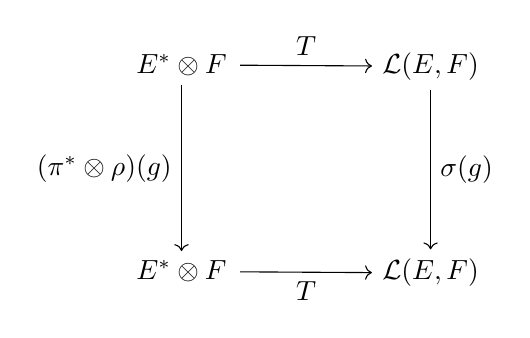
\begin{tikzpicture}
	\matrix (m) [matrix of math nodes, row sep=5.8em, column sep=4.8em, minimum width=4.2em]
	{
		E^*\otimes F & \mathcal{L}(E,F) \\ 
		E^*\otimes F & \mathcal{L}(E,F) \\ 
	};
	\path[->]
	(m-1-1) edge node [above] {$T$} (m-1-2)
	edge node [left] {$(\pi^*\otimes \rho)(g)$} (m-2-1)
	(m-1-2) edge node [auto]  {$\sigma(g)$} (m-2-2)
	(m-2-1) edge node [below] {$T$} (m-2-2)
	;
	\end{tikzpicture} \quad \quad \quad \, 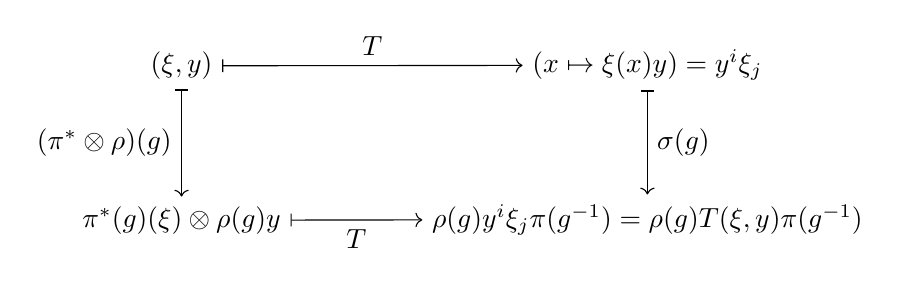
\begin{tikzpicture}
	\matrix (m) [matrix of math nodes, row sep=3.8em, column sep=4.8em, minimum width=2.2em]
	{
		(\xi,y) & (x\mapsto \xi(x) y) = y^i \xi_j \\
		\pi^*(g)(\xi) \otimes \rho(g)y & \rho(g) y^i \xi_j \pi(g^{-1}) = \rho(g) T(\xi,y) \pi(g^{-1}) \\
	};
	\path[|->]
	(m-1-1) edge node [above] {$T$} (m-1-2)
	edge node [left] {$(\pi^*\otimes \rho)(g)$} (m-2-1)
	(m-1-2) edge node [auto]  {$\sigma(g)$} (m-2-2)
	(m-2-1) edge node [below] {$T$} (m-2-2)
	;
	\end{tikzpicture}
	Thus, representation $\sigma(g)$ is equivalent to representation $(\pi^*\otimes \rho)$, a tensor product of representations.  
	
\end{enumerate}

\exercisehead{2.15} \emph{Representation of $GL(2, \mathbb{C})$ on the polynomials of degree 2}

Let group $G$, let representation $\rho$ of $G$ on $V= \mathbb{C}^n$, i.e. $\rho : G \to \text{End}(V)$ \\
Let $P^{(k)}(V)$ vector space of complex polynomials on $V$ that are homogeneous of degree $k$. 

For $f\in P^{(k)}(V)$, the general form is 
\[
f = \sum_{ \substack{ i_1 + i_2 + \dots + i_n = k \\ 0 \leq i_j \leq k } } a_{i_1 i_2 \dots i_d} x_1^{i_1} x_2^{i_2} \dots x_n^{i_n}
\]

Given 
\[
\binom{n+k}{k} = \binom{k-1}{k-1} + \binom{k}{k-1} + \dots + \binom{n+k-1}{k-1} = \sum_{i=0}^n \binom{k-1+i}{k-1}
\]
$\binom{k+n-1}{n-1}$ is number of monomials of degree $k$.  

So $\text{dim}P^{(k)}(V) = \binom{k+n-1}{n-1}$.   This is a very lucid and elementary exposition on the basics of polynomials which I found was useful for the basic facts I forgot\footnote{Polynomials. Math 4800/6080 Project Course \url{http://www.math.utah.edu/~bertram/4800/PolyIntroduction.pdf}}.

So we have the graded algebra
\[
P(V) = \bigoplus_{k=0}^{\infty} P^{(k)}(V)
\]

\[
\begin{aligned}
& \rho^{(k)}: G \to \text{End}(P^{(k)}(V)) \\ 
& \rho^{(k)}(g): P^{(k)}(V) \to P^{(k)}(V) \\ 
& \rho^{(k)}(g)(f) = f\circ \rho(g^{-1})
\end{aligned}
\]
This is a representation of $G$ since 
\begin{enumerate}
	\item[(a)] 
	\[
	\begin{gathered}
	\begin{aligned}
	& \rho^{(k)}(gh)(f) = f\circ \rho((gh)^{-1}) = f\circ \rho(h^{-1}g^{-1}) = f\circ \rho(h^{-1}\rho(g^{-1}) \\ 
	& \rho^{(k)}(g) \rho^{(k)}(h)(f) = \rho^{(k)}(g) (f\circ \rho(h^{-1})) = f\circ \rho(h^{-1})\circ \rho(g^{-1})
	\end{aligned} \Longrightarrow \rho^{(k)}(gh) = \rho^{(k)}(g) \rho^{(k)}(h)
	\end{gathered}
	\]
	
	
	\item[(b)]
	Choose basis $(e_1 \dots e_n)$ of $V$, $x = x^j e_j \in V$, $\rho : G \to \text{End}(V)$, and so $\rho(g)(x) = \rho(g)(x^je_j) = x^j\rho(g)(e_j)= x^j(\rho(g))^i_{ \,\, j} e_i$.  \\
	With $\xi(e_i) = \xi_i \Longrightarrow \langle \xi, \rho(g^{-1})x\rangle = \xi_i x^j (\rho(g^{-1}))^i_{ \,\, j}$
	
	$\forall \, \xi \in V^*$, $\xi = \xi_i e^i$, 
	\[
	\begin{gathered}
	\rho^*(g)(\xi) = \rho^*(g)(\xi_i e^i) = \xi_i \rho^*(g)^i_{\,\,j} e^j \\ 
	\Longrightarrow   \langle \rho^*(g)(\xi), x \rangle = \xi_i x^j (\rho^*(g))^i_{ \,\,j} \Longrightarrow (\rho^*(g))^i_{\,\,j} = (\rho(g^{-1}))^i_{ \,\, j} 
	\end{gathered}
	\]
	
	So $\forall \, f \in P^{(1)}(V)$, $x\in V$, $\rho(g^{-1})x = x^j(\rho(g^{-1}))^i_{\,\,j} e_i$.  So $f\circ \rho(g^{-1})(x) = \sum_{i=1}^n a_i(\rho(g^{-1}))^i_{\,\,j} x^j = \sum_{i=1}^n a_i(\rho^*(g))^i_{\,\,j} x^j$ \\
	$\Longrightarrow \rho^{(1)}(g)(f) = f\circ \rho^*(g)$
	\item[(c)] Suppose $G= GL(2,\mathbb{C})$, $V=\mathbb{C}^2$, $\rho$ fundamental representation $g= \left( \begin{matrix} a & b \\
	c & d \end{matrix} \right)$, $g^{-1} = \frac{1}{\text{det}g} \left( \begin{matrix} d & -b \\
	-c & a \end{matrix} \right)$ for $\text{det}g = ad-bc$.  
	
	Let $k=2$, $\text{dim}P^{(2)}(\mathbb{C}^2) = \binom{2+2-1}{2-1} = \binom{3}{1} = 3$
	
	$\forall \, f \in P^{(2)}(\mathbb{C}^2)$, $f(x,y) = Ax^2 + 2Bxy + Cy^2$ \\
	Let 
	\[
	\begin{gathered}
	P^{(2)}(\mathbb{C}^2) \to \mathbb{C}^3 \\ 
	f(x,y) = Ax^2 + 2Bxy + Cy^2 \mapsto \left( \begin{matrix} A \\ B \\ C \end{matrix} \right) \in \mathbb{C}^3
	\end{gathered}
	\]
	Call this transformation $T$, $T: P^{(2)}(\mathbb{C}^2) \to \mathbb{C}^3$.  
	
	$\forall \, \left( \begin{matrix} A \\ B \\ C \end{matrix} \right) \in \mathbb{C}^3$, $f(x,y) = Ax^2 + 2Bxy + Cy^2$ and $Tf(x,y) = \left( \begin{matrix} A \\ B \\ C \end{matrix} \right)$.  $T$ surjective.  
	
	Suppose $Tf(x,y) = Tf'(x,y)$, 
	\[
	\begin{gathered}
	\Longrightarrow Ax^2 + 2Bxy + Cy^2 = A'x^2 + 2B'xy + C'y^2 \\ 
	\Longrightarrow (A-A')x^2 + 2(B-B')xy + (C-C')y^2 = 0
	\end{gathered}
	\]
	Then since the monomials form a basis, and its basis elements are independent (by definition), then $A=A'$, $B=B'$, $C=C'$.  $T$ injective.  So $T$ is bijective, an isomorphism.  
	
	(This is all in \verb|groups.sage|)
	\begin{lstlisting}
	sage: P2CC.<x,y> = PolynomialRing(CC,2) # this declares a PolynomialRing of field of complex numbers, 
	# of order 2 (i.e. only 2 variables for a polynomial, such as x, y)
	sage: A = var('A')
	sage: assume(A,''complex'')
	sage: B = var('B')
	sage: assume(B,''complex'')
	sage: C = var('C')
	sage: assume(C,''complex'')
	sage: f(x,y) = A*x**2 +2*B*x*y + C*y**2
	
	sage: a = var('a')
	sage: assume(a,''complex'')
	sage: b = var('b')
	sage: assume(b,''complex'')
	sage: c = var('c')
	sage: assume(c,''complex'')
	sage: d = var('d')
	sage: assume(d,''complex'')
	sage: g = Matrix([[a,b],[c,d]] )
	sage: X = Matrix([[x],[y]])
	sage: f( (g.inverse()*X)[0,0], (g.inverse()*X)[1,0] ).expand()
	sage: f( (g.inverse()*X)[0,0], (g.inverse()*X)[1,0] ).expand().coefficient(x^2).full_simplify()
	(C*c^2 - 2*B*c*d + A*d^2)/(b^2*c^2 - 2*a*b*c*d + a^2*d^2)
	sage: f( (g.inverse()*X)[0,0], (g.inverse()*X)[1,0] ).expand().coefficient(x*y).full_simplify()
	-2*(C*a*c + A*b*d - (b*c + a*d)*B)/(b^2*c^2 - 2*a*b*c*d + a^2*d^2)
	sage: f( (g.inverse()*X)[0,0], (g.inverse()*X)[1,0] ).expand().coefficient(y^2).full_simplify()
	(C*a^2 - 2*B*a*b + A*b^2)/(b^2*c^2 - 2*a*b*c*d + a^2*d^2)
	\end{lstlisting}
	
	So 
	\[
	\begin{gathered}
	\rho^{(2)}(g)(f)(x,y) = f\circ \rho(g^{-1})(x,y) = \\
	= \frac{ Cc^2 - 2Bcd + Ad^2}{(ad-bc)^2}x^2 + - 2 \frac{ (Cac + Abd - (bc+ad) B)}{(ad-bc)^2} xy + \frac{ Ca^2 - 2Bab + Ab^2 }{(ad-bc)^2 } y^2
	\end{gathered}
	\]
	
	So define $\widetilde{ \rho}: G \to \text{End}(\mathbb{C}^3)$. $\widetilde{\rho}$ is a representation, for 
	\[
	\begin{gathered}
	\forall v = \left( \begin{matrix} A \\ B \\ C \end{matrix} \right) \in \mathbb{C}^3, \quad \, \widetilde{\rho}(gh)(v) = T \circ f \circ \rho((gh)^{-1}) = T\circ f \circ \rho(h^{-1}g^{-1}) = T\circ f \circ \rho(h^{-1}) \rho(g^{-1}) \\ 
	\text{ Now } \widetilde{\rho}(h)(v) = T\circ f \circ \rho(h^{-1}) \\
	\Longrightarrow \widetilde{\rho}(g) \widetilde{\rho}(h)(v) = T \circ (f\circ \rho(h^{-1}))\circ \rho(g^{-1}) = T\circ f \circ \rho(h^{-1}) \rho(g^{-1}) \text{ and so }\\
	\widetilde{\rho}(gh) = \widetilde{\rho}(g) \widetilde{\rho}(h)
	\end{gathered}
	\]
	
	And so 
	\[
	\widetilde{\rho}^*(g)(v) = Tf\rho(g^{-1})
	\]
	and consider this commutation diagram, that (helped me at least and) clarifies the relationships:
	
	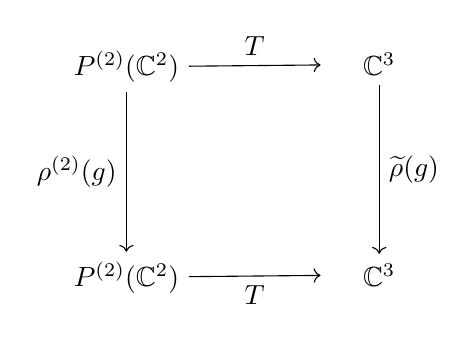
\begin{tikzpicture}
	\matrix (m) [matrix of math nodes, row sep=5.8em, column sep=4.8em, minimum width=4.2em]
	{
		P^{(2)}(\mathbb{C}^2) & \mathbb{C}^3 \\ 
		P^{(2)}(\mathbb{C}^2) & \mathbb{C}^3 \\ 
	};
	\path[->]
	(m-1-1) edge node [above] {$T$} (m-1-2)
	edge node [left] {$\rho^{(2)}(g)$} (m-2-1)
	(m-1-2) edge node [auto]  {$\widetilde{\rho}(g)$} (m-2-2)
	(m-2-1) edge node [below] {$T$} (m-2-2)
	;
	\end{tikzpicture} \quad \quad \quad \, 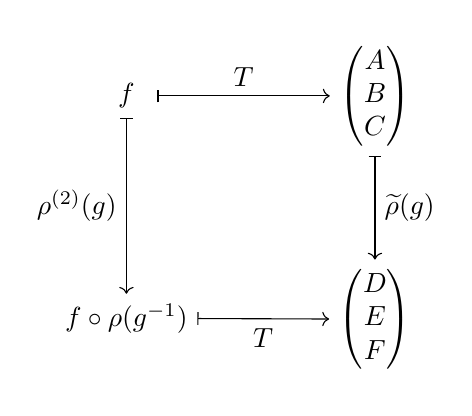
\begin{tikzpicture}
	\matrix (m) [matrix of math nodes, row sep=3.8em, column sep=4.8em, minimum width=2.2em]
	{
		f & \left( \begin{matrix} A \\ B \\ C \end{matrix} \right) \\ 
		f\circ \rho(g^{-1}) & \left( \begin{matrix} D \\ E \\ F \end{matrix} \right) \\ 
	};
	\path[|->]
	(m-1-1) edge node [above] {$T$} (m-1-2)
	edge node [left] {$\rho^{(2)}(g)$} (m-2-1)
	(m-1-2) edge node [auto]  {$\widetilde{\rho}(g)$} (m-2-2)
	(m-2-1) edge node [below] {$T$} (m-2-2)
	;
	\end{tikzpicture}
	
	with
	\[
	\left( \begin{matrix} D \\ E \\ F \end{matrix} \right) = \left( \begin{matrix} \frac{ Cc^2 - 2Bcd + Ad^2}{(ad-bc)^2} \\ 
	- 2 \frac{ (Cac + Abd - (bc+ad) B)}{(ad-bc)^2} \\
	\frac{ Ca^2 - 2Bab + Ab^2 }{(ad-bc)^2 } \end{matrix} \right)
	\]
	
	Now define the dual $\widetilde{\rho}^*$ as such:
	\[
	\begin{gathered}
	\begin{aligned}
	& \widetilde{\rho}^*(g): (\mathbb{C}^3)^* \to (\mathbb{C}^3)^* \\ 
	&  \widetilde{\rho}^*(g) = \widetilde{\rho}(g^{-1}) 
	\end{aligned}  \\
	\begin{gathered}
	\forall \, \xi \in (\mathbb{C}^3)^* \\ 
	\widetilde{\rho}^*(g)\xi = \xi_i (\widetilde{\rho}^*(g))^i_{ \,\, j} e^j = \xi_i (\widetilde{\rho}(g^{-1}))^i_{ \,\, j} e^j
	\end{gathered}
	\end{gathered}
	\]
	
	So for $v = \left( \begin{matrix} A \\ B \\ C \end{matrix} \right) \in \mathbb{C}^3$, $f = T^{-1}v = Ax^2 + 2Bxy + Cy^2 \in P^2(\mathbb{C}^2)$, 
	\[
	\widetilde{\rho}(g^{-1})(v) = T \circ ( f \rho(g) ) = \left[ \begin{matrix} Aa^2 + 2Bac + Cc^2 \\
	Aab + Bbc + Bad + Ccd \\
	Ab^2 + 2Bbd + Cd^2 \end{matrix} \right]
	\]
	which was found using Sage Math:
	\begin{lstlisting}
	sage: f((g*X)[0,0],(g*X)[1,0])
	(a*x + b*y)^2*A + 2*(a*x + b*y)*(c*x + d*y)*B + (c*x + d*y)^2*C
	sage: f((g*X)[0,0],(g*X)[1,0]).expand()
	A*a^2*x^2 + 2*B*a*c*x^2 + C*c^2*x^2 + 2*A*a*b*x*y + 2*B*b*c*x*y + 2*B*a*d*x*y + 2*C*c*d*x*y + A*b^2*y^2 + 2*B*b*d*y^2 + C*d^2*y^2
	sage: f((g*X)[0,0],(g*X)[1,0]).expand().coefficient(x^2)
	A*a^2 + 2*B*a*c + C*c^2
	sage: f((g*X)[0,0],(g*X)[1,0]).expand().coefficient(x*y)
	2*A*a*b + 2*B*b*c + 2*B*a*d + 2*C*c*d
	sage: f((g*X)[0,0],(g*X)[1,0]).expand().coefficient(y^2)
	A*b^2 + 2*B*b*d + C*d^2
	\end{lstlisting}
	or 
	\begin{lstlisting}
	sage: T( f((g*X)[0,0],(g*X)[1,0]).expand() )
	[A*a^2 + 2*B*a*c + C*c^2,
	2*A*a*b + 2*B*b*c + 2*B*a*d + 2*C*c*d,
	A*b^2 + 2*B*b*d + C*d^2]
	\end{lstlisting}
	
	So then 
	\[
	\widetilde{\rho}(g^{-1}) = \left[ \begin{matrix} a^2 & 2ac & c^2 \\ 2ab & 2(ad+bc) & 2cd \\ b^2 & 2bd & d^2 \end{matrix} \right]
	\]
	So then 
	\[
	\widetilde{\rho}^*(g) = \left[ \begin{matrix} a^2 & 2ac & c^2 \\ 2ab & 2(ad+bc) & 2cd \\ b^2 & 2bd & d^2 \end{matrix} \right]
	\]
	and operate on row vectors $\xi \in (\mathbb{C}^3)^*$ with $\widetilde{\rho}^*(g)$ from the row vector's right.  
\end{enumerate}

More: Let $G = SU(2)$.  Then $U = e^{i\phi} \left[ \begin{matrix} a & b \\ -\overline{b} & \overline{a} \end{matrix} \right]$

\[
\begin{gathered}
\begin{aligned}
& \widetilde{\rho} : SU(2) \to \text{End}(\mathbb{C}^3) \\
& \widetilde{\rho}(U) : \mathbb{C}^3 \to \mathbb{C}^3 \\
& \widetilde{\rho}(U)(v) = e^{-2i\varphi} \left[ \begin{matrix} A\overline{a}^2 + 2B\overline{a}\overline{b} + C \overline{b}^2 \\ 
-A\overline{a}b + B + Ca\overline{b} \\
Ab^2 - 2Bab + Ca^2 \end{matrix} \right]
\end{aligned} \\
\Longrightarrow \widetilde{\rho}(U) = e^{-2i \varphi} \left[ \begin{matrix} -\overline{a}^2 & 2\overline{a}\overline{b} & \overline{b}^2 \\
-\overline{a}b & 1 & a\overline{b} \\
b^2 & - 2ab & a^2 \end{matrix} \right]
\end{gathered}
\]

cf. Ch. 5 Lie Groups of Jeffrey Lee (2009) \cite{JLee2009}

\begin{definition}[Lie Group]
\textbf{Lie Group} $G :=$ smooth manifold $G$ is a \textbf{Lie Group} if $G$ is a group (abstract group), s.t. \\
multiplication map $\begin{aligned} & \quad \\ 
& \mu : G \times G \to G \\
& \mu(g,h) = gh \end{aligned}$ \\
inverse map $\begin{aligned} & \quad \\ 
& \text{inv} : G \to G \\
& \text{inv}(g) = g^{-1} \end{aligned}$ \\
are $C^{\infty}$ maps.

If group is abelian, use additive notation $g+h$ for group operation.
\end{definition}

\begin{definition}[$GL(n, \mathbb{R})$]
	$GL(n,\mathbb{R}) := $ group of all invertible real $n\times n$ matrices. 
	
	global chart on $GL(n, \mathbb{R}) = \lbrace x^i_j \rbrace$, $n^2$ functions $x^i_j$, where if $A \in GL(n,\mathbb{R})$, then $x^i_j(A)$ is $ij$th entry of $A$. 
\end{definition}

\emph{Claim}: $GL(n,\mathbb{R})$ is a Lie group. 

\begin{proof}
multiplication is clearly smooth: $(AB)_{ij} = A_{ik}B_{kj}$, 
\[
\begin{gathered}
	\frac{ \partial }{ \partial x^l_m} (x^i_k(A) x^k_j(B)) = \delta^i_l \delta^m_k x^k_j(B) + x^i_k(A)\delta^k_l \delta^m_j
\end{gathered}
\]
inversion map; appeal to formula for $A^{-1}$, $A^{-1} = \text{adj}(A) / \text{det}(A)$, $\text{adj}(A) \equiv$ adjoint matrix (whose entries are cofactors). \\
$\Longrightarrow A^{-1}$ depends smoothly on entries of $A$.

Similarly, $GL(n,\mathbb{C})$, group of invertible $n\times n$ complex matrices, is a Lie group.
\end{proof}

\exercisehead{5.5}\label{Ex:5.5SubgroupIsOpenAndClosed} Let subgroup $H$ of $G$, consider cosets $gH$, $g\in G$.

Recall $G$ is disjoint union of cosets of $H$.

\emph{Claim}: if $H$ open, so are all its cosets. And $H$ closed.

\begin{proof}
	cf. \href{https://math.stackexchange.com/questions/226847/open-subgroups-of-a-topological-group-are-closed}{stackexchange: Open subgroups of a topological group are closed}
	
	$gH = \lbrace gh | h \in H \rbrace$ is an open neighborhood of $g$ (since $1 \in H$, and mapping $h \mapsto gh$ sends open sets to open sets, since its inverse, $gh \mapsto h$, is $C^{\infty}$ (so continuous)).
	
	\[
	\begin{gathered}
	\begin{aligned}
	& gH \to H \\
	& gh \xrightarrow{g^{-1}} h = \mu(g^{-1}, gh)
	\end{aligned} \qquad \, 
	\begin{aligned}
	& H \to gH \\
	& h \xrightarrow{g} gh = \mu(g, h) 
	\end{aligned}
	\end{gathered}
	\]
	
	Then $\forall \, $ coset $gH$, $gH$ is open.
	
	Suppose $g' \in H^c \equiv G-H \equiv G\backslash H$.
	
	Consider $h\in H$, if $g'h \in H$, then $g' = (g'h)h^{-1} \in H$ (recall $h^{-1} \in H$, and $H$ is a subgroup).
	
	Contradiction.
	
	$\Longrightarrow \forall \, g' \in H^c$, $\exists \, $ open neighborhood $g'H \subset H^c$, so $H^c$ open (by definition). Then $H$ closed.
	
	\end{proof}

cf. Thm. 5.6 in Jeffrey Lee (2009) \cite{JLee2009}.
\begin{theorem}
	If $G$ connected Lie group, $U$ neighborhood of identity element $e$, then $U$ generates the group, i.e. $\forall \, g \in G$, $g$ is a product of elements of $U$.
\end{theorem}

\begin{proof}
	Note $V = \text{inv}(U) \cap U$ is an open neighborhood of $e$. Note $\text{inv}(V) =V$. $\text{inv}(V) \equiv V^{-1} = \lbrace V^{-1} | v \in V \rbrace$. We say that $V$ is \emph{symmetric}.
	
	\emph{Claim}: $V$ generates $G$.
	
	$\forall \, $ open $W_1$, open $W_2\subset G$, \\
	$W_1W_2 = \lbrace w_1 w_2 | w_1 \in W_1, w_2 \in W_2 \rbrace$ is an open set being a union of open sets $\bigcup_{g\in W_1} gW_2$.
	
	Thus, inductively defined sets
	\[
	V^n = VV^{n-1}, \quad \, n = 1,2,3,\dots
	\]
	are open.
	
	\[
	e \in V \subset V^2 \subset \dots V^n \subset \dots
	\]
	
	It's easy to check that each $V^n$ is symmetric.
	\[
	\begin{gathered}
	\begin{aligned}
	& \text{inv}(V) = V \\
	& \text{inv}(V^2) = \text{inv}( \bigcup_{v\in V} vV) = V \text{inv}(V) = V = V^2 \\
	& \text{inv}(V^{n+1}) = \text{inv}\left( \bigcup_{v\in V} vV^n \right) = V \text{inv}(V^n) = VV^n = V^{n+1}
	\end{aligned}
	\end{gathered}	
	\]
	so $V^{\infty} := \bigcup_{n=1}^{\infty} V^n$ is symmetric.

$V^{\infty}$ closed under inversion, also multiplication. Thus $V^{\infty}$ is an open subgroup.

From Exercise 5.5, Jeffrey Lee (2009) \cite{JLee2009}, i.e. Exercise \ref{Ex:5.5SubgroupIsOpenAndClosed}, $V^{\infty}$ also closed, since $G$ is connected, $V^{\infty} = G$. (a topological space $X$ is \textbf{connected} iff the only open and closed (clopen) sets are $\emptyset$ and $X$).
	
\end{proof}

\begin{definition}
	Identity component of $G, G_0$.  

$G_0 := $ connected component of Lie group $G$ that contains identity; \\
$G_0$ is a Lie group, and is generated by any open neighborhood of the identity.
\end{definition}

\begin{definition}
	For Lie group $G$, fixed element $g\in G$, \\
	left translation (by $g$) $L_g: G \to G$, $L_g x  = gx$, \quad \, $\forall \, x \in G$ \\
	right translation (by $g$) $R_g: G \to G$, $R_g x  = xg$, \quad \, $\forall \, x \in G$ 
\end{definition}

$L_g$, $R_g$ are diffeomorphisms with $L_g^{-1} = L_{g^{-1}}$, $R_g^{-1} = R_{g^{-1}}$.

\begin{definition}[Product Lie group]
	If $G,H$ are Lie groups, then product manifold $G\times H$ is a Lie group, where multiplication
	\[
	(g_1, h_1) \cdot (g_2, h_2) = (g_1g_2, h_1h_2)
	\]
	Lie group $G\times H$ is called \textbf{product Lie group}
\end{definition}
e.g. product group $S^1 \times S^1 \equiv $ 2-torus group.

Generally, higher torus groups $T^n = S^1 \times \dots \times S^1$ ($n$ factors).

\begin{definition}[Lie subgroup of $G$, $H$]
	Let $H$ be an abstract subgroup of Lie group $G$. 
	
	If $H$ is a Lie group s.t. inclusion map $i: H \to G \equiv H \hookleftarrow G$ is an immersion, then $H$ is a 

	\textbf{Lie subgroup} of $G$.
\end{definition}
Recall $i : H \to G$ immersion iff $Di$ injective, i.e.	iff $\text{rank}{Di} = \text{dim}{H}$


cf. Prop. 5.9 in Jeffrey Lee (2009) \cite{JLee2009}.
\begin{proposition}
	If $H$ abstract subgroup of Lie group $G$, that's also a regular submanifold $\equiv$ embedded submanifold, then $H$ closed Lie subgroup.
\end{proposition}

%\begin{proof}
%	$H$ subgroup of $G$, so \\
%	multiplication map $H\times H \to H$ \\
%	inversion map $H \to H$ 
	
%	are restrictions of multiplication and inversion maps on $G$.
%\end{proof}

\emph{Recall that} 
\begin{quote}
	\emph{embedded submanifold} $\equiv $ \emph{regular submanifold}
\end{quote}
Each name is used frequently and we shouldn't be biased against one or the other; we'll have to refer to both, to emphasize they're \emph{exactly the same}.

embedded submanifold $\equiv $ regular submanifold is an immersed submanifold s.t. inclusion map $i$ is a topological embedding, \\
i.e. embedded submanifold $\equiv $ regular submanifold $S \subset M$,  \\
immersed submanifold $S$ if $i:S \to M \equiv S \hookrightarrow M$ is an immersion, i.e. $Di$ injective, i.e. $\text{rank}Di \equiv \text{dim}S$. \\
topological embedding $:=$ homeomorphism onto its image, i.e. \\
\qquad \, injective cont. map $f:X \to Y$, $X, Y$ topological spaces, is a \textbf{topological embedding} \\
\qquad \qquad \, if $f$ is a homeomorphism between $X$ and $f(X)$.  \\
\qquad \qquad \qquad \, $f$ homeomorphism is a bijection, continuous, and $f^{-1}$ continuous. \\

e.g. $\forall \, $ embedding $f: M \to N$, $f(M) \subset N$ naturally has the structure of an embedding submanifold $\equiv $ regular submanifold.

\emph{Useful, intrinsic definition} of \textbf{embedded submanifold} $\equiv$ regular submanifold. \\
Let manifold $M$, $\text{dim}M = n$, let $k \in \mathbb{Z}^+$, s.t. $0\leq k \leq n$.

A $k$-dim. embedded submanifold $\equiv $ regular submanifold $S$ is subset $S \subset M$ s.t. $\forall \, p \in S$, $\exists \, $ chart ($U\subset M, \, \varphi : U \to \mathbb{R}^n \ni 0$), s.t. $\varphi(S \cap U)$ is the intersection of a $k$-dim. plane with $\varphi(U)$.  \\
 (pairs ($S\cap U, \left. \varphi \right|_{S \cap U})$ form an atlas for differential structure on $S$).

Proof 1:

\begin{proof}
$H$ subgroup of $G$, so \\
multiplication map $H\times H \to H$ \\
inversion map $H\to H$ \\
are restrictions of multiplication and inversion maps on $G$.

\qquad \\
Since $H$ regular submanifold, maps are smooth. \\
Recall $H$ regular submanifold iff $H$ immersive submanifold (i.e. $H\hookleftarrow G$ is an immersion) and $H$ topological subspace of $G$, i.e. submanifold topology on $H$ is same as subspace topology.

\quad \\ 
Claim: $H$ closed. \\
Let $x_0 \in \overline{H}$ \\
Let $(U,x)$ be a chart adapted to $H$, whose domain contains $e$. \\
Let 
\[
\begin{aligned}
& \delta : G \times G \to G \\
& \delta (g_1, g_2)  = g_1^{-1} g_2
\end{aligned}
\]

\quad \\ 
Choose open set $V$ s.t. $e\in V \subset \overline{V} \subset U$. \\
By continuity map $\delta$, find open neighborhood $O$ of identity $e$ s.t. $O \times O \subset \delta^{-1}(V)$ \\
If $\lbrace h_i \rbrace$ sequence in $H$ converging to $x_0 \in \overline{H}$, then $x_0^{-1} h_i \to e$ and $x_0^{-1} h_i \in O$ for all sufficiently large $i$.  \\
Since $h_j^{-1} h_i = (x_0^{-1} h_j)^{-1} x_0^{-1} h_i$, $h_j^{-1} h_i \in V$ for sufficiently large $i,j$.  \\

For any sufficiently large fixed $j$, 
\[
\lim_{i\to 0} h_j^{-1} h_i = h_j^{-1} x_0 \in \overline{V} \subset U
\]
Since $U$ is domain of a single-slice chart, $U\subset H$ closed in $U$.

\quad \\
Thus, since $\forall \, h_j^{-1} h_i \in U \cap H$, $h_j^{-1} x_0 \in U \cap H \subset H$, \quad \, $\forall \, $ sufficiently large $j$.  \\
$\Longrightarrow x_0 \in H$, and since $x_0$ arbitrary, done.
	
	
	\end{proof}

Proof 2:

cf. 9.2 The Closed Subgroup Theorem I of 427 Notes\footnote{\url{https://faculty.math.illinois.edu/~lerman/519/s12/427notes.pdf}}

\begin{proof}

	\textbf{Claim}: Since $H$ is an embedded submanifold $\equiv $ regular submanifold, $\exists \, $ neighborhood $U$ of 1, $1 \in G$, s.t. $U\cap H$ closed in $U$. 
	
	\qquad \, \\
	Let $x_0 \in \overline{H}$, $\overline{H} \equiv $ closure of $x_0$. \\
	Then $x_0U^{-1} \subseteq G$ is a neighborhood of $x_0$ in $G$ (since $1 \in U^{-1}$, $x_0 1 = x_0 \in x_0 U^{-1}$)
	\[
	\Longrightarrow x_0 U^{-1} \cap H \neq \emptyset 
	\]
	$\forall \, x \in x_0 U^{-1} \cap H$, $x= x_0 U^{-1}$ for some $u\in U$. Thus, $x^{-1} x_0 = u \in U$.
	
	\quad \\
	Now  \\
	$L_{x^{-1}} : G \to G$ is a homeomorphism, so $L_{x^{-1}}(H) = H$. By continuity, $L_{x^{-1}}(\overline{H}) = \overline{H}$. Thus $x^{-1}x_0 \in \overline{H}$. 
	
	\textbf{Claim}: $x^{-1} x_0 \in H \cap U$. \\
	Since $x^{-1}x_0 \in \overline{H} \cap U$, $\exists \, $ sequence $\lbrace h_i \rbrace \subset H \cap U$ s.t. $h_0 \to x^{-1} x_0$. \\
	But recall $H\cap U$ closed in $U$, so $x^{-1}x_0 \in H\cap U$. 
	\[
	\Longrightarrow x_0 \in xH = H , \quad \, \overline{H} \subseteq H
	\]
	Thus $H$ closed. 

	\quad \\ 	
	\textbf{Claim}: If $H$ abstract subgroup of Lie group $G$, that's also an embedded submanifold $\equiv$ regular submanifold, then $H$ is a Lie subgroup. 
	
	\quad \\ 
	Recall that by definition, Lie group has group multiplication and inverse map to be $C^{\infty}$. Then, just show group multiplication is $C^{\infty}$, first.

\quad \\	
Since $G$ is a Lie group, then
\[
\begin{gathered}
\begin{aligned}
& \mu : G \times G \to G \\
& \mu(x,y) = xy
\end{aligned}
\end{gathered}
\]	
is $C^{\infty}$ (by definition).

\quad \\ 
Then $\mu : G \times G \to G$ cont.  \\
Consider subgroup $H\subseteq G$ and $\mu : H \times H \to H$. \\
Since $H\times H \subseteq G \times G$, $\forall \, (x,y) \in H \times H$ (fix $(x,y) \in H\times H$), $\forall \, $ neighborhood $V$ of $\mu(x,y) = xy$, $V\subset G$, $\exists \, $ neighborhood $U$ of $(x,y)$ s.t. $\mu(U) \subseteq V$ (by $\mu: G \times G \to G$ cont.).

Since $H$ embedded submanifold $\equiv $ regular submanifold of $G$,  \\
\qquad \, $\exists \, $ neighborhood $V' \subseteq V$ of $xy \in G$, coordinate map $\varphi:V' \to \mathbb{R}^n$ ($n = \text{dim}G$) s.t.
\[
\varphi(H \cap V') = \varphi(V') \cap (\mathbb{R}^k \times \lbrace 0 \rbrace)
\]
where $k = \text{dim}H$	
	
(since $H$ is a $k$-dim. embedded submanifold $\equiv$ regular submanifold, $H\subseteq G$, s.t. $\forall \, p \in H$, $\exists $ chart ($V \subset G, \, \varphi : U \to \mathbb{R}^n \ni 0$), s.t. $\varphi(U \cap V) = \varphi(V) \cap (\mathbb{R}^k \times \lbrace 0 \rbrace)$).

Now \\
\[
\varphi \circ \mu : \mu^{-1}(V') \cap U \to \mathbb{R}^n \text { is } C^{\infty}, \text{ and } \varphi \circ \mu(\mu^{-1}(V') \cap U) \subseteq \mathbb{R}^k \times \lbrace 0 \rbrace 
\]	

Let projection $\pi : \mathbb{R}^n \to \mathbb{R}^k$ be the standard projection, 
\[
\pi \circ \varphi \circ \mu : \mu^{-1}(V') \cap U \to \mathbb{R}^k \text{ is } C^{\infty}
\]
	
$\Longrightarrow \mu $ is $C^{\infty}$	
\end{proof}




From Chapter 4 ``Lie Groups and Lie Algebras'' of Kosmann-Schwarzbach (2010) \cite{YKosmann-Schwarzbach2010}

While Proposition 2.6 of Kosmann-Schwarzbach (2010) \cite{YKosmann-Schwarzbach2010} states that
\[
\text{det}(\exp(X)) = \exp{ (\text{tr}{X} ) }
\]
here are some other resources online that gave further discussion on the characteristic polynomial, $\text{det}(A-\lambda 1)$ and the different terms of it, called Newton identities:
\begin{itemize}
	\item \url{http://scipp.ucsc.edu/~haber/ph116A/charpoly_11.pdf}
	\item \url{http://math.stackexchange.com/questions/1126114/how-to-find-this-lie-algebra-proof-that-mathfraksl-is-trace-zero-matrice}
	\item \url{http://mathoverflow.net/questions/131746/derivative-of-a-determinant-of-a-matrix-field}
\end{itemize}

\begin{theorem}[5.1 \cite{YKosmann-Schwarzbach2010}]\label{Thm:5.1YKos}
	Consider $\mathfrak{g} = \lbrace X = \gamma'(0) | \gamma : 1 \to G \text{ of class $C^1$ }, \, \gamma(0) = 1 \rbrace$ \\
	Let Lie group $G$
	\begin{enumerate}
		\item[(i)] $\mathfrak{g}$ vector subspace of $\mathfrak{gl}(n,\mathbb{R})$
		\item[(ii)] $X \in \mathfrak{g}$ iff $\forall \, t \in \mathbb{R}$, $\exp{(tX)} \in G$ 
		\item[(iii)] if $X \in \mathfrak{g}$, if $g\in G$, then $gXg^{-1} \in \mathfrak{g}$
		\item[(iv)] $\mathfrak{g}$ closed under matrix commutator, i.e. if $X,Y \in \mathfrak{g}$, $[X,Y] \in \mathfrak{g}$
	\end{enumerate}
\end{theorem}

\begin{proof}
	\begin{enumerate}
		\item[(i)]
		\item[(ii)] If $\exp{ (tX)} \in G$, then $X \left. \frac{d}{dt} \exp{(tX)} \right|_{t=0} \in \mathfrak{g}$ (by def.)
		
		If $X \in \mathfrak{g}$, then by def., $X = \left. \frac{d}{dt} \gamma(t) \right|_{t=0}$ with $\gamma(t) \in G$.  
		
		Now Taylor expand; $\forall \, k \in \mathbb{Z}^+$ 
		
		\[
		\begin{gathered}
		\gamma\left( \frac{t}{k} \right) = 1 + \frac{t}{k} X + O\left( \frac{1}{k^2} \right) = \exp{ \left( \frac{t}{k} X + O\left( \frac{1}{k^2} \right) \right) } \\
		\Longrightarrow \left( \gamma \left( \frac{t}{k} \right) \right)^k = \exp{ (tX)}
		\end{gathered}
		\]
		
		\[
		\gamma\left( \frac{t}{k} \right) \in G \quad \, \forall \, k \in \mathbb{Z}^+
		\]
		$G$ closed subgroup, so $\lim_{k \to \infty} (\gamma\left( \frac{t}{k} \right) )^k = \exp{(tX) } \in G$
		\item[(iii)]
		\item[(iv)]
	\end{enumerate}
\end{proof}

\begin{definition}[Lie algebra]
	Lie algebra $\mathfrak{g}$, tangent space to $G$ at $1$, i.e. $\mathfrak{g} := T_1 G$ is called \emph{Lie algebra} of Lie group $G$.  
	
	\[
	\mathfrak{g} := \lbrace X = \gamma'(0) | \gamma: 1 \to G \text{ of class $C^1$ }, \gamma(0) = 1 \rbrace = T_1G
	\]
\end{definition}

This is based on  Proposition 5.3 of Kosmann-Schwarzbach (2010) \cite{YKosmann-Schwarzbach2010}.  

For Lie group 
\[
U(n) = \lbrace U \in GL(n,\mathbb{C}) | UU^{\dag} = 1 \rbrace
\]
If $X \in \mathfrak{u}(n)$, then $\exp{(tX)} \in U(n)$.  Then
\[
\exp{(tX)} \exp{(tX)}^{\dag} = (1+tX + O(t^2) )(1+tX^{\dag} + O(t^2) ) = 1 + t(X+X^{\dag}) +O(t^2) = 1 \forall \, t\in \mathbb{R} \Longrightarrow X+X^{\dag} = 0 
\]
i.e. $X \in \mathfrak{u}(n)$ is an anti-Hermitian complex $n\times n$ matrix.  

$\mathfrak{u}(n) = \lbrace X \in \mathfrak{gl}(n,\mathbb{C}) | X + X^{\dag} =0 \rbrace$

\emph{Physicists}: $X = iA$ and so $A-A^{\dag}$.  $A \in \mathfrak{u}(n)$ is a Hermitian complex $n\times n$ matrix.  

$\mathfrak{u}(n) = \lbrace A \in \mathfrak{gl}(n,\mathbb{C}) | A - A^{\dag} =0 \rbrace$

Regardless, $\text{dim}_{\mathbb{R}}\mathfrak{u}(n) = n^2 = 2n^2 - n^2$

For Lie group 
\[
SU(n) = \lbrace  U \in GL(n,\mathbb{C}) | UU^{\dag} = 1 , \text{det}U = 1 \rbrace
\]
Then
\[
\mathfrak{su}(n) = \lbrace X \in \mathfrak{gl}(n,\mathbb{C}) | X + X^{\dag} = 1 , \, \text{tr}{X} = 0 \rbrace
\]
is the Lie algebra of traceless anti-Hermitian complex $n\times n$ matrices, and that 
\[
\text{dim}_{\mathbb{R}}\mathfrak{su}(n) = n^2 - 1 
\]

In summary, 

\[
\begin{gathered}
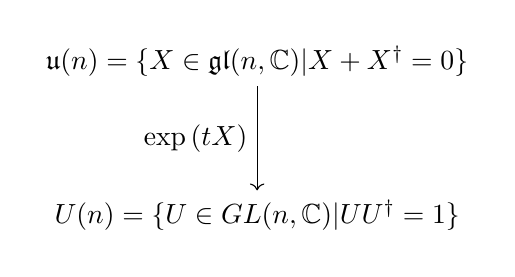
\begin{tikzpicture}
\matrix (m) [matrix of math nodes, row sep=3.8em, column sep=4.8em, minimum width=2.2em]
{
	\mathfrak{u}(n) = \lbrace X \in \mathfrak{gl}(n,\mathbb{C}) | X + X^{\dag} =0 \rbrace \\  
	U(n) = \lbrace U \in GL(n,\mathbb{C}) | UU^{\dag} = 1 \rbrace \\  
};
\path[->]
(m-1-1) edge node [left] {$\exp{(tX)}$} (m-2-1)
;
\end{tikzpicture} \quad \quad \, 
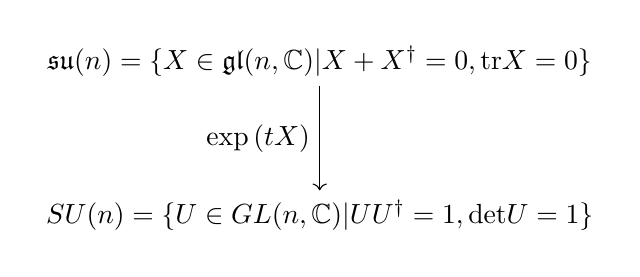
\begin{tikzpicture}
\matrix (m) [matrix of math nodes, row sep=3.8em, column sep=4.8em, minimum width=2.2em]
{
	\mathfrak{su}(n) = \lbrace X \in \mathfrak{gl}(n,\mathbb{C}) | X + X^{\dag} =0, \text{tr}{X}=0 \rbrace \\ 
	SU(n) = \lbrace U \in GL(n,\mathbb{C}) | UU^{\dag} = 1, \text{det}U=1 \rbrace \\ 
};
\path[->]
(m-1-1) edge node [left] {$\exp{(tX)}$} (m-2-1)
;
\end{tikzpicture} \\
\text{dim}_{\mathbb{R}} \mathfrak{u}(n) = n^2   \quad \quad \quad \, \text{dim}_{\mathbb{R}}\mathfrak{su}(n) = n^2-1
\end{gathered}
\]

From Chapter 5 ``Lie Groups $SU(2)$ and $SO(3)$'' of Kosmann-Schwarzbach (2010) \cite{YKosmann-Schwarzbach2010}, 

\subsubsection{Bases of $\mathfrak{su}(2)$, Subsection 1.1 of Chapter 5of Kosmann-Schwarzbach (2010) \cite{YKosmann-Schwarzbach2010}}

Recall that 

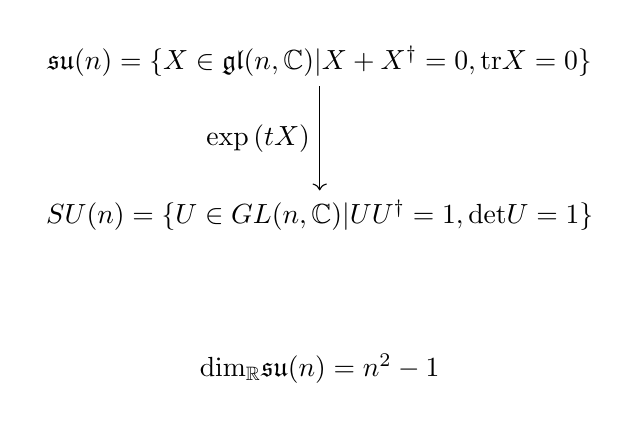
\begin{tikzpicture}
\matrix (m) [matrix of math nodes, row sep=3.8em, column sep=4.8em, minimum width=2.2em]
{
	\mathfrak{su}(n) = \lbrace X \in \mathfrak{gl}(n,\mathbb{C}) | X + X^{\dag} =0, \text{tr}{X}=0 \rbrace \\ 
	SU(n) = \lbrace U \in GL(n,\mathbb{C}) | UU^{\dag} = 1, \text{det}U=1 \rbrace \\ 
	\text{dim}_{\mathbb{R}}\mathfrak{su}(n) = n^2-1 \\
};
\path[->]
(m-1-1) edge node [left] {$\exp{(tX)}$} (m-2-1)
;
\end{tikzpicture} 

and so 

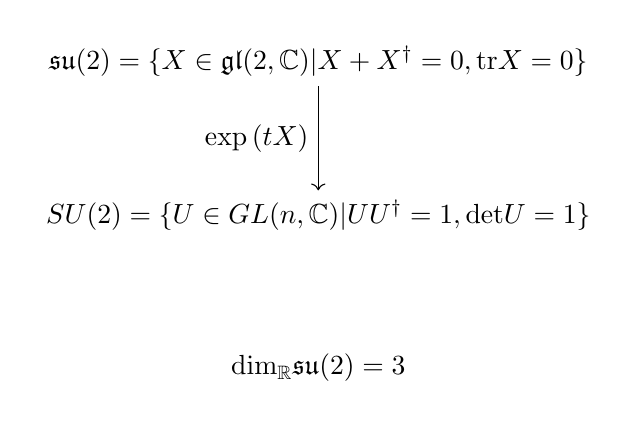
\begin{tikzpicture}
\matrix (m) [matrix of math nodes, row sep=3.8em, column sep=4.8em, minimum width=2.2em]
{
	\mathfrak{su}(2) = \lbrace X \in \mathfrak{gl}(2,\mathbb{C}) | X + X^{\dag} =0, \text{tr}{X}=0 \rbrace \\ 
	SU(2) = \lbrace U \in GL(n,\mathbb{C}) | UU^{\dag} = 1, \text{det}U=1 \rbrace \\ 
	\text{dim}_{\mathbb{R}}\mathfrak{su}(2) = 3 \\
};
\path[->]
(m-1-1) edge node [left] {$\exp{(tX)}$} (m-2-1)
;
\end{tikzpicture} 

Also, recall that $\mathfrak{g} \subseteq \mathfrak{gl}(n,\mathbb{C})$ is a vector subspace (\ref{Thm:5.1YKos}) and that \\
$X \in \mathfrak{g}$ iff $\forall t \in \mathbb{R}$, $\exp{(tX)} \in G$.  \\
if $X \in \mathfrak{g}$, if $g\in G$, then $gXg^{-1} \in \mathfrak{g}$ \\
$\mathfrak{g}$ closed under $\begin{aligned} & \quad \\
& \mathfrak{g} \times \mathfrak{g} \to \mathfrak{g} \\
& (X,Y) \mapsto [X,Y] \end{aligned}$

and so with $\mathfrak{g}$ as a vector space, we can have a choice of bases.  

\begin{enumerate}
	\item[(a)] $\begin{aligned}
	& \xi_1 = \frac{i}{2} \left( \begin{matrix} & 1 \\ 1 & \end{matrix} \right) \\ 
	& \xi_2 = \frac{1}{2} \left( \begin{matrix} & -1 \\ 1 & \end{matrix} \right) \\
	& \xi_3 = \frac{i}{2} \left( \begin{matrix} 1 &  \\  & -1 \end{matrix} \right) 
	\end{aligned}$
	
	satisfying 
	
	\[
	[\xi_k , \xi_l ] = \epsilon_{klm} \xi_m
	\]
	\item[(b)] \emph{Physics}
	
	$\begin{aligned}
	& \sigma_1 = -2i \xi_1 =  \left( \begin{matrix} & 1 \\ 1 & \end{matrix} \right) \\ 
	& \sigma_2 = 2i \xi_2 =  \left( \begin{matrix} & -i \\ i & \end{matrix} \right) \\
	& \sigma_3 = -2i \xi_3 =  \left( \begin{matrix} 1 &  \\  & -1 \end{matrix} \right) 
	\end{aligned}$
\end{enumerate}

satisfying 

\[
[ \sigma_k, \sigma_l ] = 2i \epsilon_{klm} \sigma_m
\]

EY : 20151001 Sage Math 6.8 doesn't run on Mac OSX El Capitan: I suspect that it's because in Mac OSX El Capitan, \verb|/usr| cannot be modified anymore, even in an Administrator account.  The TUG group for MacTeX had a clear, thorough, and useful (i.e. copy UNIX commands, paste, and run examples) explanation of what was going on:

\url{http://tug.org/mactex/elcapitan.html}

So keep in mind that my code for Sage Math is for Sage Math 6.8 that doesn't run on Mac OSX El Capitan.  I'll also use \verb|sympy| in Python as an alternative and in parallel.  

One can check in \verb|sympy| the traceless anti-Hermitian (or Hermitian) property of the bases and Pauli matrices, and the commutation relations (see \verb|groups.py|):

\begin{lstlisting}
import itertools
from itertools import product, permutations

import sympy
from sympy import I, LeviCivita
from sympy import Rational as Rat

from sympy.physics.matrices import msigma # <class 'sympy.matrices.dense.MutableDenseMatrix'>

def commute(A,B):
"""
commute = commute(A,B)
commute takes the commutator of A and B
"""
return (A*B - B*A)

def xi(i):
"""
xi = xi(i)
xi is a function that returns the independent basis for 
Lie algebra su(2)\equiv su(2,\mathbb{C}) of Lie group SU(2) of 
traceless anti-Hermitian matrices, based on msigma of sympy
cf. http://docs.sympy.org/dev/_modules/sympy/physics/matrices.html#msigma
"""
if i not in [1,2,3]:
raise IndexError("Invalid Pauli index")
elif i==1:
return I/Rat(2)*msigma(1)
elif i==2:
return -I/Rat(2)*msigma(2)
elif i==3:
return I/Rat(2)*msigma(3)

\end{lstlisting}

\begin{lstlisting}
## check anti-Hermitian property and commutation relations with xi 
# xi is indeed anti-Hermitian
xi(1) == -xi(1).adjoint() # True
xi(2) == -xi(2).adjoint() # True
xi(3) == -xi(3).adjoint() # True

# xi obeys the commutation relations

for i,j in product([1,2,3],repeat=2): print i,j

for i,j in product([1,2,3],repeat=2): print i,j, "\t Commutator: ", commute(xi(i),xi(j))

## check traceless Hermitian property and commutation relations with Pauli matrices
# Pauli matrices i.e. msigam is indeed traceless Hermitian

msigma(1) == msigma(1).adjoint() # True
msigma(2) == msigma(2).adjoint() # True
msigma(3) == msigma(3).adjoint() # True

msigma(1).trace() == 0 # True
msigma(2).trace() == 0 # True
msigma(3).trace() == 0 # True

# Pauli matrices obey commutation relation
print "For Pauli matrices, the commutation relations are :\n"
for i,j in product([1,2,3],repeat=2): print i,j, "\t Commutator: ", commute(msigma(i),msigma(j))

for i,j,k in permutations([1,2,3],3): print "Commute: ", i,j,k, msigma(i), msigma(j), \ \
": and is 2*i of ", msigma(k), commute(msigma(i),msigma(j)) == 2*I*msigma(k)*LeviCivita(i,j,k)

\end{lstlisting}

And finally the traceless property of the Pauli matrices:
\begin{lstlisting}
>>> msigma(1).trace()
0
>>> msigma(2).trace()
0
>>> msigma(3).trace()
0
\end{lstlisting} 

\subsection{Rotation Group $SO(N)$ and Lie Algebra $\textbf{so}(3)$}

cf. Kambe (2009) \cite{TKambe2009}, Appendix C

$g \in SO(N)$ represented by $N\times N$ orthogonal matrix (i.e. $gg^T = 1$) s.t. $\text{det}g = 1$. \\

Let curve $\xi(t)$ on $SO(N)$, initially from identity $1$, with tangent vector $\mathbf{a}$ at $1$.

$\Longrightarrow \xi(t) = 1 + t\mathbf{a} + O(t^2)$ for an infinitesimal parameter $t$.

$\mathbf{a} = \xi'(0)$ is an element of tangent space $T_1 SO(N)$ i.e. the Lie algebra $\mathbf{so}(N)$, i.e. $T_1SO(N) = \mathbf{so}(N)$ by orthogonality condition $\xi(t) \xi^T(t) = 1$, then
\begin{equation}\label{Eq:SO(N)LieAlgebraIsSkewSymmetric}
(1 + t\mathbf{a} + \dots ) (1 + t\mathbf{a}^T + \dots )  = 1 \Longrightarrow \mathbf{a} + \mathbf{a}^T = 0 \text{ or } \mathbf{a} = \mathbf{a}^T
\end{equation}
$\Longrightarrow  \mathbf{a}$ skew-symmetric.

\subsubsection{$\mathbf{so}(3)$}

$\text{dim}(\mathbf{so}(3)) = 3$, vector space of Lie algebra $\mathbf{so}(3)$ represented by skew-symmetric basis $(E_1, E_2, E_3)$
\[
\begin{gathered}
E_1 = \left[ \begin{matrix} 0 & 0 & 0 \\ 0 & 0 & -1 \\ 0 & 1 & 0 \end{matrix} \right] \, , \quad \, E_2 = \left[ \begin{matrix} 0 & 0 & 1 \\ 0 & 0 & 0 \\ -1 & 0 & 0 \end{matrix} \right] \, , \quad \, E_3 = \left[ \begin{matrix} 0 & -1 & 0 \\ 1 & 0 & 0 \\ 0 & 0 & 0 \end{matrix} \right] \\
[E_i , E_j ] =\epsilon_{ijk}E_k \text{ where } [E_i, E_j ] = E_i E_j - E_j E_i
\end{gathered} 
\]



\subsection{Spin}

Let's follow the development by Baez and Muniain (1994) on pp. 175 of the Section II.1 ``Lie Groups'', the second (II) chapter on ``Symmetry'' \cite{JBaezJMuniain1994}.  

Let $V = \mathbb{C}^2$, $G=SU(2)$.  Then consider the graded algebra of polynomials on $V = \mathbb{C}^2 \ni (x,y)$
\[
\begin{gathered}
P(V) = \bigoplus_{k=0}^{\infty} P^{(k)}(V) = \bigoplus_{ \substack{ j =0 \\ 2j \in \mathbb{Z}} }^{\infty} P^{(2j)}(V) = \bigoplus_{ \substack{ j=0 \\ j\in \mathbb{Z} }}^{\infty} P^{(2j)}(V) \oplus \bigoplus_{ \substack{ j=1/2 \\ 2j \text{ odd } } }^{\infty} P^{(2j)}(V) \\
P^{(2j)}(V) \equiv \text{ vector space of complex polynomials of degree $2j$ }
\end{gathered}
\]
and recall this representation on $P^{(2j)}(V)$
\[
\begin{aligned}
& \rho^{(2j)}:G \to \text{End}(P^{(2j)}(V)) \\ 
& \rho^{(2j)}: P^{(2j)}(V) \to P^{(2j)}(V) \\ 
& \rho^{(2j)}(g)(f) = f\circ \rho(g^{-1}) \text{ where $\rho$ is the fundamental representation of $G=SU(2)$ }\\
& \rho^{(2j)}(g)(f)(v) = f\circ \rho(g^{-1})(v) \quad \, \forall \, f \in P^{(2j)}(V), \, \forall \, v \in V = \mathbb{C}^2
\end{aligned}
\]
Note, \\
$\text{dim}P^{(2j)} = \binom{2j+2-1 }{2-1} = 2j+1$

\exercisehead{21} \cite{JBaezJMuniain1994} \emph{spin-0} Consider the trivial representation $\tau$:
\[
\begin{aligned}
& \tau : G \to \text{End}(\mathbb{C}) \\ 
& \tau(g): \mathbb{C} \to \mathbb{C} \\ 
& \tau(g) = 1_{\mathbb{C}}
\end{aligned} \quad \quad \,  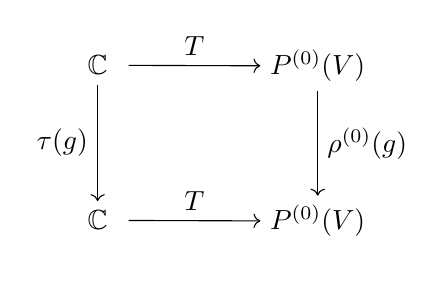
\begin{tikzpicture}
\matrix (m) [matrix of math nodes, row sep=3.8em, column sep=4.8em, minimum width=2.2em]
{
	\mathbb{C} & P^{(0)}(V) \\ 
	\mathbb{C} & P^{(0)}(V) \\ 
};
\path[->]
(m-1-1) edge node [above] {$T$} (m-1-2)
edge node [left] {$\tau(g)$} (m-2-1)
(m-1-2) edge node [auto]  {$\rho^{(0)}(g)$} (m-2-2)
(m-2-1) edge node [auto] {$T$} (m-2-2)
;
\end{tikzpicture}
\]

Clearly, $P^{(0)}(V) = \mathbb{C}$, since $P^{(0)}(V)$ consists of polynomials of constants in $\mathbb{C}$.  

Consider $c_0 \in \mathbb{C}$, $f = k_0 \in P^{(0)}(V)$ \\
$\rho^{(0)}(g)(f) = f\circ \rho(g^{-1}) = k_0$ \\
$\Longrightarrow \rho^0(g)T(c_0) = T\circ \tau(g) c_0 = T(c_0)$.  Let $T = 1_{\mathbb{C}} = 1_{P^{0}(V)}$

So $\rho^{(0)}(g) = \tau(g) = 1$.  $T=1$.  So representations $\rho^{(0)}$ and trivial representation $\tau$ on $G$ are equivalent.  



\exercisehead{22} \cite{JBaezJMuniain1994} \emph{spin-$\frac{1}{2}$} For spin-$\frac{1}{2}$, $j=\frac{1}{2}$, $2j=1$.  

$\forall \, f \in P^{(1)}(V)$, $V = \mathbb{C}^2$.  So in general form, $f(x,y) = ax + by \in P^{(1)}(V)$, $\left( \begin{matrix} x \\ y \end{matrix} \right) \in V = \mathbb{C}^2$  

Recall the fundamental representation $\begin{aligned} & \quad \\
& \rho : G \to GL(2,\mathbb{C}) \equiv GL(\mathbb{C}^2) \\
& \rho(g) : \mathbb{C}^2 \to \mathbb{C}^2 \\
& \rho(g) = g \end{aligned}$

So consider $T$ such that 

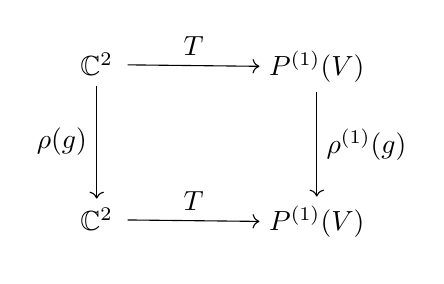
\begin{tikzpicture}
\matrix (m) [matrix of math nodes, row sep=3.8em, column sep=4.8em, minimum width=2.2em]
{
	\mathbb{C}^2 & P^{(1)}(V) \\ 
	\mathbb{C}^2 & P^{(1)}(V) \\ 
};
\path[->]
(m-1-1) edge node [above] {$T$} (m-1-2)
edge node [left] {$\rho(g)$} (m-2-1)
(m-1-2) edge node [auto]  {$\rho^{(1)}(g)$} (m-2-2)
(m-2-1) edge node [auto] {$T$} (m-2-2)
;
\end{tikzpicture}

Consider $\forall \, v \in \mathbb{C}^2$, $v =\left( \begin{matrix} x \\ y \end{matrix} \right)$, then 
\[
\rho(g)v = gv = \left[ \begin{matrix} ax + by \\ cx + dy \end{matrix} \right]
\]

\begin{lstlisting}
sage: g*X
[a*x + b*y]
[c*x + d*y]
\end{lstlisting}

For notation, let $U \in G = SU(2)$ s.t. $UU^{\dag}=1$.  

Consider $(\rho^{(2j)}(U)(f))(x) = f(U^{-1}x)$, $\forall \, x \in \mathbb{C}^2$.  

Choose $f(x,y) = x$.  So for $f(x,y) = Ax+By$, $A=1,B=0$.  Choose $U = \left( \begin{matrix} a & b \\
-\overline{b} & \overline{a} \end{matrix} \right)$ so $U^{-1} = \left( \begin{matrix} \overline{a} & -b \\
\overline{b} & a \end{matrix} \right)$.  Then $U^{-1}x = \left( \begin{matrix} \overline{a}x - by \\
\overline{b}x + ay \end{matrix} \right)$

So 
\[
\begin{aligned}
& (\rho^{(1)}(U)(f) )(x) = f(U^{-1}x) = \overline{a}x - by \\ 
& (\rho^{(1)}(U)(f))(x) = f(U^{-1}x) = \overline{b}x + ay \text{ for } f(x,y) = y 
\end{aligned}
\]
Let $f(x,y) = Ax + By$
\[
\begin{gathered}
(\rho^{(1)}(U)(f))(x) = f(U^{-1}x) = (A\overline{a}+B\overline{b})x + (Ba - Ab)y = (\overline{a}x - by)A + (\overline{b}x + ay)B  = (A\overline{a} + B\overline{b})x + (Ba-Ab)y
\end{gathered}
\]
which was calculated with the assistance of Sage Math:
\begin{lstlisting}
sage: U_try1 = Matrix( [[a.conjugate(),-b],[b.conjugate(),a ] ] )
sage: f1( U_try1*X).coefficient(x)
A*conjugate(a) + B*conjugate(b)
sage: f1( U_try1*X).coefficient(y)
B*a - A*b
\end{lstlisting}

Treating $P^{(1)}(\mathbb{C}^2)$ as a vector space, in its matrix formulation, then $f(x,y) = Ax+By \in P^{(1)}(\mathbb{C}^2)$ is treated as $\left[ \begin{matrix} A \\ B \end{matrix} \right]$, then $(\rho^{(1)}(U)f)$ is 
\[
\Longrightarrow \left[ \begin{matrix} \overline{a} & \overline{b} \\ -b & a \end{matrix} \right]\left[ \begin{matrix} A \\ B \end{matrix} \right] = \left[ \begin{matrix} A\overline{a} + B\overline{b}  \\ -Ab + Ba \end{matrix} \right]
\]
so conclude in general that $\rho^{(1)}(U) = (U^{\dag})^T$.  

Now, as Kosmann-Schwarzbach (2010) \cite{YKosmann-Schwarzbach2010} says, on pp. 13, Chapter 2 Representations of Finite Groups, ``Two representations $(E_1,\rho_1)$ and $(E_2,\rho_2)$ are equivalent if and only if there is a basis $B_1$ of $E_1$ and a basis $B_2$ of $E_2$ such that for every $g\in G$, the matrix of $\rho_1(g)$ in the basis $B_1$ is equal to the matrix of $\rho_2(g)$ in the basis $B_2$.  In particular, if the representations $(E_1,\rho_1)$ and $(E_2,\rho_2)$ are equivalent, then $E_1$ is isomorphic to $E_2$.''  So we need a change of basis between $\rho(U) = U$ and $\rho^{(1)}(U)$.  What's the linear transformation $T$ s.t.
\[
T^{-1} \rho^{(1)}(U) T = U ?
\]  
By intuition, 
\[
T = \sigma_x \sigma_z \equiv \sigma_1 \sigma_3
\]
where $\sigma_i$'s are Pauli matrices.  

Indeed, 
\begin{lstlisting}
sage: Paulimat[3] * Paulimat[1]*U_try*Paulimat[1] * Paulimat[3]
[conjugate(a) conjugate(b)]
[          -b            a]
\end{lstlisting}

Then $\rho^{(1)}(U)\circ T = TU$, so this $T = \sigma_1 \sigma_3$ is an ``intertwining operator'' between $\rho^{(1)}(U)$ and fundamental representation $\rho(U) = U$, with $T = \left[ \begin{matrix} & - 1 \\
1 & \end{matrix} \right]$, and $T^{-1} = \left[ \begin{matrix} & 1 \\ -1 & \end{matrix} \right]$.  

$T$ is an isomorphism between $\mathbb{C}^2$ and $P^{(1)}(\mathbb{C}^2)$.  So fundamental representation $\rho$ of $G=SU(2)$ is equivalent to $\rho^{(1)}(U)$ on $P^{(1)}(\mathbb{C}^2)$.  

\exercisehead{23}\cite{JBaezJMuniain1994} (Also from Exercise 2.6 of Kosmann-Schwarzbach (201) \cite{YKosmann-Schwarzbach2010})

Let $(E,\pi)$ representation of group $G$.  \\
$\forall \, g \in G$, $\xi \in E^*$, $x\in E$, set $\langle \pi^*(g)(\xi), x \rangle = \langle \xi, \pi(g^{-1})(x) \rangle$

\emph{dual} (or \emph{contragredient}) of $\pi$, $\pi^*:G \to \text{End}(E^*)$, $\pi^*$ is a representation, since
\[
\begin{gathered}
\langle \pi^*(gh)(\xi),x\rangle = \langle \xi, \pi((gh)^{-1})(x) \rangle = \langle \xi, \pi(h^{-1}g^{-1})(x) \rangle = \langle \xi, \pi(h^{-1}) \pi(g^{-1})(x) \rangle = \langle \xi, \pi(h^{-1}) (\pi(g^{-1})(x)) \rangle =  \\
= \langle \pi^*(h)(\xi), \pi(g^{-1})(x) \rangle = \langle \pi^*(g)\pi^*(h)(\xi), x \rangle
\end{gathered}
\]
since this is true, $\forall \, x \in E$, $\forall \, \xi \in E^*$, $\pi^*(gh) = \pi^*(g)\pi^*(h)$.  

dual $\pi^*$ of $\pi$ is a representation.  


\subsection{Adjoint Representation}

I will first follow Sec. 7.3 The Adjoint Representation of Ch. 4 Lie Groups and Lie Algebras of Kosmann-Schwarzbach (201) \cite{YKosmann-Schwarzbach2010}).  

The \emph{conjugation action} $\mathcal{C}_g:G\to G$ is defined as 
\[
\begin{aligned}
& \mathcal{C}_g:G\to G \\
&  \mathcal{C}_g: h \mapsto ghg^{-1}
\end{aligned}
\]
So 
\[
\begin{aligned}
& \mathcal{C}: G \to \text{Aut}(G) \\ 
& \mathcal{C}g = \mathcal{C}_g
\end{aligned}
\]
Now define the \emph{adjoint action} of $g$ as the differential or push forward of $\mathcal{C}_g$:
\[
\text{Ad}_g := D_1 \mathcal{C}_g \equiv (\mathcal{C}_g)_{*1} \equiv \left. (\mathcal{C}_g )_* \right|_{g=1}  \qquad \, (\text{adjoint action of $g$})
\]
Now $\text{Ad}_g: \mathfrak{g} \to \mathfrak{g}$, so $\begin{aligned} & \quad \\
& \text{Ad}:G \to \text{End}(\mathfrak{g}) \\
& \text{Ad}(g) \equiv \text{Ad}_g \end{aligned}$

Note $\mathcal{C}_{gg'} = \mathcal{C}_g \mathcal{C}_{g'} \equiv \mathcal{C}(gg') = \mathcal{C}(g)\circ \mathcal{C}(g')$ and so 
\[
\xrightarrow{ D_1} \text{Ad}_{gg'} = \text{Ad}_g \circ \text{Ad}_{g'}
\]

Kosmann-Schwarzbach (201) \cite{YKosmann-Schwarzbach2010}) claims, because $\text{Ad}_g = 1_{\mathfrak{g}}$ when $g=1$, 

$\begin{aligned} & \quad \\
& \text{Ad}:G \to GL(\mathfrak{g}) \\
& \text{Ad}:g\mapsto \text{Ad}_g\end{aligned}$ is a representation of $G$ on $\mathfrak{g}$.   (EY : 20160505 ???)

\begin{definition}
	representation $\text{Ad}$ of $G$ on $V=\mathfrak{g}$ is called adjoint representation of Lie group $G$.  
\end{definition}

Denote adjoint representation of Lie algebra $\mathfrak{g}$, $\text{ad}$.  

By definition, $\text{Ad}_{\text{exp}(tX)} = \exp{ (t\text{ad}_X)}$

cf. Prop. 7.8 of Kosmann-Schwarzbach (201) \cite{YKosmann-Schwarzbach2010})
\begin{proposition}
	\begin{enumerate}
		\item Let $A$ invertible matrix, $A \in $ Lie group $G$.  \\
		Let $X$ matrix s.t. $X \in \mathfrak{g}$.  Then
		\[
		\text{Ad}_A(X) = AXA^{-1}
		\]
		\item Let $X,Y \in \mathfrak{g}$.  Then 
		\[
		\text{ad}_X(Y) = [X,Y]
		\]
		\item Let $X,Y \in \mathfrak{g}$.  Then 
		\[
		\text{ad}_{[X,Y]} = [ \text{ad}_X, \text{ad}_Y ]
		\]
	\end{enumerate}
\end{proposition}
\begin{proof}
	\begin{enumerate}
		\item By def., $\forall \, B \in G$, $\mathcal{C}_A(B) = ABA^{-1}$, and thus
		\[
		\text{Ad}_A(X) = \left. \frac{d}{dt} A\exp{ (tX)  }A^{-1} \right|_{t=0} = AXA^{-1}
		\]
		\item \[
		\begin{gathered}
		\text{ad}_X(Y) = \left. \frac{d}{dt} \text{Ad}_{\exp{(tX)}}(Y) \right|_{t=0} = \left. \frac{d}{dt} \exp{(tX)} Y \exp{(tX)} \right|_{t=0} = \\
		= XY - YX = [X,Y] 
		\end{gathered}
		\]
		\item Use Jacobi identity: 
		\[
		\begin{gathered}
		[A,[B,C]] +  [B,[C,A]] +  [C,[A,B]] = 0 \text{ or } \\ 
		[[A,B],C] = [A,[B,C]] - [B,[A,C]]
		\end{gathered}
		\] 
		\[
		\begin{gathered}
		\text{ad}_{[X,Y]}C = [[X,Y],C] = [X,[Y,C]] - [Y,[X,C]] = [X,\text{ad}_YC] - [Y,\text{ad}_XC] \text{ and that } \\ 
		\text{ad}_X\text{ad}_Y C = [X,[Y,C]] \Longrightarrow \text{ad}_{[X,Y]}C = [\text{ad}_X,\text{ad}_Y ] C
		\end{gathered}
		\]
	\end{enumerate}
\end{proof}

\subsection{Invariant Vector Fields, Left-invariant Vector Field, Right-invariant Vector Field, Invariant Vector Fields}

cf. pp. 26, Sec. 1.7 Lie Group and Invariant Vector Fields, Kambe (2009) \cite{TKambe2009}

Consider group $G$ of smooth transformations (maps) of a manifold $M$ into itself, i.e. Lie group. \\

Given fixed element $h \in G$, then
\begin{equation}
\begin{aligned}
& L_h : g\mapsto hg \text{ i.e. } L_h(g) = hg \\
& R_h : g \mapsto gh \text{ i.e. } R_h(g) = gh
\end{aligned}
\end{equation}
where 
$ \begin{aligned} & \quad \\
& L_h \equiv \text{ left translation of the group } \\
& R_h \equiv \text{ right translation of the group } 
\end{aligned}$

Suppose $g_t$ is a curve on $G$ described in terms of parameter $t$. \\
Left translation of $g_t$ by $g_{\Delta t}$ for infinitesimal $\Delta t$ given by $g_{\Delta t} \circ g_t$. 
\begin{equation}
	\dot{g}_t = \lim_{\Delta t \to 0} \frac{g_{t + \Delta t} - g_t }{ \Delta t } = \lim_{\Delta t \to 0} \frac{ (g_{\Delta t} - 1) g_t }{ \Delta t} = X \circ g_t \text{ with } X := \lim_{\Delta t \to 0 } \frac{ g_{\Delta t} - 1}{ \Delta t}  \in T_1 G
\end{equation}

Thus, left translation $L_{g_{\Delta t}} $ leads to \textbf{right}-invariant vector field. \\
Similarly, right translation $R_{g_{\Delta t}}$ leads to \textbf{left}-invariant vector field. \\
In summary,


$\dot{g}_t$ is said to be tangent vector at $g_t$.

Vector field $X^L, (X^R)$ on $G$ is left invariant (right invariant) if it's invariant under all left-translations (right translations) respectively, i.e. $\forall \, g,h \in G$, if 

\begin{equation}
\begin{aligned}
	& (L_h)_* X^L_g = X^L_{hg} \\
	& (R_h)_* X^R_g = X^R_{hg} 	
\end{aligned}
\end{equation}

Given tangent vector $X$ to $G$, at $e$, one may left-translate (right translate) $X$ to every pt. $g\in G$ as 
\begin{equation}\label{Eq:LeftRightTranslatePushForwardResultsInLeftRightInvariantFields}
\begin{aligned}
	& X^L_g = (L_g)_* X = g\circ X = gX \\
	& X^R_g = (R_g)_* X = X\circ g = Xg 
\end{aligned}	
\end{equation}

Since
\[
\begin{gathered}
	(R_h)_* X^R_g = (R_h)_*(R_g)_* X = X\cdot gh = X^R_{gh}
\end{gathered}
\]
Then $(R_h)_*$ operation does yield a right-invariant field.

Hence $(R_h)_*$ transformation in Eq. \ref{Eq:LeftRightTranslatePushForwardResultsInLeftRightInvariantFields} gives a right-invariant field generated by $X$. 

In other words, in summary
\begin{equation}\label{Eq:LeftTranslationRightInvariantVectorField}
\begin{gathered}
\text{ Left translation of  $g_t$ by $g_{\Delta t}$: } \begin{aligned}
& L_{g_{\Delta t}} : g_t \mapsto g_{\Delta t} g_t = g_{t+\Delta t } \\
& \dot{g}_t = X g_t  \text{ so } X \in T_1G \text{ is right-invariant vector field }
\end{aligned} \\
\text{ i.e. } X^R_g = (R_g)_*X = Xg
\end{gathered}
\end{equation}

Consider curves $\begin{aligned} & \quad \\ 
	\xi_t & :   \mathbb{R} \to G \\ 
	\xi  & : t \mapsto \xi(t), \quad \, t\in \mathbb{R} \end{aligned}$ \quad \, with tangent $\dot{\xi}_0 = X$ at $t=0$.

Left-invariant field $X_s^L = \frac{d}{dt} (g\circ \xi_t)$ \quad \, $\forall \, g_s \in G$, ($s$ a parameter) \\
Right-invariant field $X_s^R = \frac{d}{dt} ( \xi_t \circ g_s)$ \\

Lie group $G$ acts as a group of linear transformations on its own Lie algebra $\mathfrak{g}$, namely \\
$\forall \, g\in G$, $\exists \, $ operator $\text{Ad}_g$ s.t. 
\begin{equation}
	\text{Ad}_g Y := (L_g)_* \circ (R_{g^{-1}})_* Y = gYg^{-1}, \quad \, \forall \, Y \in \mathfrak{g}
\end{equation}

Operator $\text{Ad}_g$ transforms $Y \in \mathfrak{g}$ into $\text{Ad}_g Y \in \mathfrak{g}$, linearly. 

Set of all such $\text{Ad}_g$, i.e. $\text{Ad}(G)$ is called the adjoint representation of $G$, an adjoint group. 

Setting $g$ to be the inverse $\xi^{-1}_t := (\xi_t)^{-1}$, \\
adjoint transformation $\text{Ad}_{\xi^{-1}_t} Y$ is a function of $t$.

Its derivative with respect to $t$ is a linear transformation from $Y$ to $\text{ad}_X Y$:
\begin{equation}
\begin{aligned}
	& \text{ad}_X Y = \left. \frac{d}{dt} \xi_t^{-1} Y \xi_t \right|_{t=0} := [X, Y] \\
	& \text{ad}_X : \mathfrak{g} \to \mathfrak{g}
\end{aligned}
\end{equation}
$\text{ad}_X $ is a linear transformation $\mathfrak{g} \to \mathfrak{g}$.





\section{Lie Groups and their Lie Algebras}

\href{https://youtu.be/mJ8ZDdA10GY}{Lie groups and their Lie algebras - Lec 13 - Frederic Schuller}, Schuller (2015) \cite{Schu2015}

\subsection{Chapter 4. Lie Theory, Schuller (2015) \cite{Schu2015}}

\subsubsection{4.1 Lie groups, Schuller (2015) \cite{Schu2015}}

\begin{definition}[Lie group, Schuller (2015) \cite{Schu2015}] A lie group $(G, \cdot )$ is 
\end{definition}

\part{Cohomology; Stoke's Theorem}

\section{Stoke's Theorem}

\begin{theorem}[Stoke's Theorem]
	Let $M$ be oriented, smooth $n$-manifold with boundary, \\
	let $\omega$ be a compactly supported smooth $(n-1)$-form on $M$, or if $\omega \in A_c^{n-1}(M)$, \\
	Then
	\begin{equation}
	\int_M d\omega = \int_{\partial M} \omega
	\end{equation} 
	If $\partial M = \emptyset$, then $\int_{\partial M} \omega = 0$
	
	$\int_{\partial M} \omega$ interpreted as $\int_{\partial M} i^*_{\partial M} \omega = \int_{\partial M} i^*\omega$ so 
	\begin{equation}
	\int_M d\omega = \int_{\partial M} i^*(\omega)
	\end{equation}
	where inclusion $i: \partial M \hookrightarrow M$
\end{theorem}

\begin{proof}
Begin with very special case: \\
Suppose $M = \mathbb{H}^n$ (upper half space), $\partial M = \mathbb{R}^{n-1}$ \\
$\omega$ has compact support, so $\exists \, R >0$ s.t. $\text{supp}\omega \subseteq $ rectangle $A=[-R,R] \times \dots \times [-R, R] \times [0,R]$.  

$\forall \, \omega \in A_c^{n-1}(\mathbb{H}^n)$
\begin{equation}
\omega = \sum_{j=1}^n (-1)^{j-1} f_j dx^1 \wedge \dots \wedge \widehat{dx}^j \wedge \dots \wedge dx^n \equiv \sum_{i=1}^n \omega_i dx^1 \wedge \dots \wedge \widehat{dx}^i \wedge \dots \wedge dx^n
\end{equation}
with Conlon (2008) \cite{Conl2008} and John Lee (2012) \cite{JLee2012}'s notation, respectively, and where $f_j$ has compact support.  

\[
i^*\omega = (f_1 \circ i) dx^2 \wedge \dots \wedge dx^n \in A_c^{n-1}(\partial \mathbb{H}^n)
\]
\[ 
\begin{aligned}
d\omega & = \sum_{i=1}^n d\omega_i \wedge dx^1 \wedge \dots \wedge \widehat{dx}^i \wedge \dots \wedge dx^n = \sum_{i,j=1}^n \frac{\partial \omega_i}{ \partial x^j} dx^j \wedge dx^1 \wedge \dots \wedge \widehat{dx}^i \wedge \dots \wedge dx^n = \\
& = \sum_{i=1}^n (-1)^{i-1} \frac{ \partial \omega_i}{ \partial x^i } dx^1 \wedge \dots \wedge dx^n
\end{aligned}
\]
i.e. (for another notation)
\[
d\omega = \left( \sum_{j=1}^n \frac{\partial f_j}{ \partial x^j} \right) dx^1 \wedge \dots \wedge dx^n \in A_c^n(\mathbb{H}^n)
\]

\[
d\omega = \left( \sum_{j=1}^n \frac{\partial f_j}{ \partial x^j} \right) dx^1 \wedge \dots \wedge dx^n \in A_c^n(\mathbb{H}^n)
\]

\[
\int_{\mathbb{H}^n} d\omega = \sum_{i=1}^n (-1)^{i-1} \int_A \frac{ \partial \omega_i}{ \partial x^i } dx^1 \wedge \dots \wedge dx^n = \sum_{i=1}^n (-1)^{i-1} \int_0^R \int_{-R}^R \dots \int_{-R}^R dx^1 \dots dx^n \frac{ \partial \omega_i}{\partial x^i}(x)
\]

We can change order of integration in each term so to do $x^i$ integration first. 

By fundamental thm. of calculus, terms for which $i\neq n$ reduce to 
\[
\begin{gathered}
\sum_{i=1}^{n-1} (-1)^{i-1} \int_0^R \int_{-R}^R \dots \int_{-R}^R \frac{\partial \omega_i}{\partial x^i}(x) dx^1 \dots dx^n = \sum_{i=1}^{n-1} (-1)^{i-1} \int_0^R \int_{-R}^R \dots \int_{-R}^R \frac{\partial \omega_i}{\partial x^i}(x) dx^i dx^1 \dots \widehat{dx}^i \dots dx^n = \\
= \sum_{i=1}^{n-1} (-1)^{i-1} \int_0^R \int_{-R}^R \dots \int_{-R}^R [\omega_i(x)]_{x^i = -R}^{x^i = R} dx^1 \dots \widehat{dx}^i \dots dx^n = 0 
\end{gathered} 
\]
because we've chosen $R$ large enough that $\omega =0 $ when $x^i = \pm R$.  
	
	
\end{proof}

\part{Pr\'{a}staro}

Pr\'{a}staro (1996) \cite{Pras1996}

\subsubsection{Affine Spaces}

cf. Sec. 1.2 - \emph{Affine Spaces} of Pr\'{a}staro (1996) \cite{Pras1996}

\begin{definition}[affine space]
  \begin{equation}
\begin{gathered}
    \text{ affine space \qquad \, } (M, \mathbf{M}, \alpha )  \\
    \text{ with } \\
    \begin{aligned}
      & M \equiv \text{ set (set of pts.) }  \\ 
      & \mathbf{M} \equiv \text{ vector space (space of free vectors) } \\
      & \alpha \equiv \mathbf{M} \times M \to M \equiv \text{ translation operator } \\
      & \alpha : (v,p ) \mapsto p' \equiv p + v
      \end{aligned}
\end{gathered}
  \end{equation}
  Note: $\alpha$ is a \textbf{transitive} action and without fixed pts. (free).

  i.e. $\forall \, p \in M$, 
  \end{definition}

$\forall \, $ pt. $O \in M$, $\alpha:(v,O) \mapsto O' \equiv O + v$, $\alpha (\cdot , O) \equiv \alpha_O \equiv \alpha(O)$.  $\alpha_O(v) = O' = O + \mathbf{v}$ \qquad \, $\forall \, O' \in M$, $\exists \, \mathbf{v} \in \mathbf{M}$ s.t. $O' = O + \mathbf{v}$ \\
$\Longrightarrow M \equiv \mathbf{M}$.

$\forall \, (O, \lbrace e_i \rbrace)_{1 \leq i \leq n }$, where $\lbrace e_i \rbrace$ basis of $\mathbf{M}$, $M \equiv \mathbf{M} = \mathbb{R}^n$ so isomorphism $M \simeq \mathbb{R}^n$ \\

i.e. $\alpha$ is \textbf{without fixed pts.}, meaning, 

Given pointed space $(M, O)$, where base pt. $O\in M$, we can associate $\forall \, p \in M$, vector $\mathbf{x} \in \mathbf{M}$, by 1-to-1 mapping $M\to \mathbf{M}$. 

So for 
\[
\begin{aligned}
& \alpha : \mathbf{M} \times M \to M \\ 
& \alpha(\mathbf{x}, p) = p' = p + \mathbf{x}
\end{aligned}
\]
Consider 
\[
\begin{gathered}
	\alpha(\mathbf{x}, O) = p = \alpha_O(\mathbf{x}) = p \Longrightarrow \exists \, \alpha_O^{-1}(p) = \mathbf{x} \in \mathbf{M}
\end{gathered}
\]

\begin{enumerate}
	\item tangent space of $M$ in $p\in M$ is vector space $T_pM \equiv (\mathbf{M}, p) \cong M$
	\item If $\mathbf{M}$ Euclidean space, affine space $(M, \mathbf{M}, \alpha)$ is Euclidean
	\item Call dim. of affine space $(M, \mathbf{M}, \alpha)$, dim. of $\mathbf{M} \equiv \text{dim}{\mathbf{M}}$
\end{enumerate}
$\lbrace \mathbf{e}_i \rbrace$ basis of $\mathbf{M}$




\begin{definition}
  $(O, \lbrace e_i \rbrace) \equiv $ affine frame.

  $\forall \, $ affine frame $(O,\lbrace e_i \rbrace)$, $\exists \, $ coordinate system $x^{\alpha} : M \to \mathbb{R}$, \\
  where $x^{\alpha}(p)$ is $\alpha$th component, in basis $\lbrace e_i \rbrace$, of vector $p-O$
  \end{definition}

\begin{proposition}[1.6, Pr\'{a}staro (1996) \cite{Pras1996}]
	$\forall \, O \in M$, we have canonical identification $M \equiv \mathbf{M}$, since
	\[
	\begin{gathered}
	\begin{aligned}
	& \alpha^{-1}_O:M \to \mathbf{M} \\
	& \alpha^{-1}_O(p) = \mathbf{x} 
	\end{aligned} \qquad \quad \, 
	\begin{aligned}
	& \alpha_O : \mathbf{M} \to M \\
	& \alpha_O: \mathbf{x} = \alpha(\mathbf{x}, O) = p
	\end{aligned}
	\end{gathered}
	\]
	Furthermore, \\
	$\forall \, $ \textbf{affine frame} $(O, \lbrace \mathbf{e}_i \rbrace)_{1\leq i \leq d}$, where $\lbrace \mathbf{e}_i \rbrace$ basis of $\mathbf{M}$, \\
	\phantom{Furthermore} $\exists \, $ isomorphism $M \cong \mathbb{R}^d$, \\
	Then, $\forall \, (O, \lbrace \mathbf{e}_i \rbrace)_{1 \leq i \leq d}$, \\
	\phantom{Then} $\exists \, $ coordinate system $x^{\alpha} : M \to \mathbb{R}$, \\
	\phantom{Then $\exists \, $} where $x^{\alpha}(p) = \alpha$th component, in basis $\lbrace \mathbf{e}_i \rbrace$, of vector $p - O$. 
	
	
	
\end{proposition}

\begin{theorem}[1.4 Pr\'{a}staro (1996) \cite{Pras1996}]
  Let $(x^{\alpha}), (\overline{a}^{\alpha})$ 2 coordinate systems correspond to affine frames $(O, \lbrace e_i \rbrace)$, $( \overline{O}, \lbrace \overline{e}_i \rbrace )$, respectively.
\begin{equation}
  \overline{x}^{\alpha} = A^{\alpha}_{ \, \, \beta} x^{\beta} + y^{\alpha}
\end{equation}
where
\[
y^{\alpha} \in \mathbb{R}^n, \qquad \, A^{\alpha}_{ \, \, \beta} \in GL(n; \mathbb{R})
\]
\end{theorem}

\begin{definition}[1.10 Pr\'{a}staro (1996) \cite{Pras1996}]
  \begin{equation}
    A(n) \equiv Gl(n,\mathbb{R}) \times \mathbb{R}^n
  \end{equation}
  affine group of dim. $n$
  \end{definition}

\begin{theorem}[1.5] symmetry group of $n$-dim. affine space, called affine group $A(M)$ of $M$.  $\exists \, $ isomorphism,
  \begin{equation}
    A(M) \simeq A(n), \qquad \, f\mapsto (f^{\alpha}_{ \, \, \beta} , y^{\alpha}) \, ; \qquad \, f^{\alpha} \equiv x^{\alpha} \circ f = f^{\alpha}_{ \, \, \beta} x^{\beta} + y^{\alpha}
  \end{equation}
cf. Eq. 1.4 Pr\'{a}staro (1996) \cite{Pras1996}
  \end{theorem}

\begin{definition}[metric]
	Let smooth manifold $M$, $\text{dim}M = n$, $\forall \, p \in M$, $\exists \, $ vector space $T_pM$, and so for 
	\begin{equation}
	\begin{aligned}
	& g_p (T_pM)^2 \to \mathbb{R} \\
	& g_p : (X_p,Y_p) \mapsto g_p(X_p,Y_p) \in \mathbb{R}
	\end{aligned}
	\end{equation}
	with $g_p$ being bilinear, symmetric (in $X_p,Y_p$), nondegenerate (i.e. if $g_p(X_p,Y_p)=0$, then $X_p$ or $Y_p=0$)
	
	Note that 
	\[
	g\in \Gamma((TM \otimes TM)^*)
	\]
	and that for $\begin{aligned} & \quad \\ 
	& X = X^i \frac{ \partial }{ \partial x^i } \\
	& Y = Y^i \frac{ \partial }{ \partial x^i } \end{aligned}$  
	so 	
	\[
	g(X,Y) = g_{ij} X^i Y^j
	\]  
	
\end{definition}

Now for 
\[
\begin{gathered}
\begin{aligned} 
& F: M \to N \\
& F: x \mapsto y = y(x) 
\end{aligned} \qquad \, \begin{aligned}
& DF \equiv F_* : T_p M \to T_{F(p)}N \\ 
&  DF : X_p \mapsto (DF) (X^j \frac{ \partial }{ \partial x^j }) = X^j \frac{\partial y^i}{\partial x^j} \frac{ \partial }{ \partial y^i}
\end{aligned}
\end{gathered}
\]
\[
\begin{gathered}
(F^* g')(X,Y) = (F^*g')(X^i \frac{ \partial }{ \partial x^i } , Y^j \frac{ \partial }{ \partial x^j} ) = (F^*g')_{ij} X^i Y^j = g'(F_*X, F_*Y) = \\
= 
\end{gathered}
\]

\part{Connections}

\section{Connections of Vector Bundles}

Morita (2001) \cite{Mori2001}

\begin{definition}[Connection in a vector bundle]
	\textbf{connection in a vector bundle} $\pi : E \to M$ over $C^{\infty}$ manifold $M$, is a bilinear map
	\[
	\nabla : \mathfrak{X}(M) \times \Gamma(E) \to \Gamma(E)
	\]
	satisfying
	\begin{enumerate}
		\item[(i)] $\nabla_{fX} s = f\nabla_X s$
		\item[(ii)] $\nabla_X(fs) = f\nabla_Xs + (Xf)s$ where $f\in C^{\infty}(M)$, $X \in \mathfrak{X}(M)$, $s\in \Gamma(E)$
	\end{enumerate}
$\nabla_Xs$ is covariant derivative of $s$ relative to $X$ (for Morita (2001)\cite{Mori2001})

Alternatively, Jost (2017) \cite{Jost2017} defines in the following way: \\

Let vector bundle $(E, \pi, M)$, where differentiable manifold $M$, vector bundle $E$ over $M$; a covariant derivative or (linear) connection is map
\begin{equation}
	D:\Gamma(E) \to \Gamma(E) \otimes \Gamma(T^*M) \equiv \Gamma(E) \otimes \mathfrak{X}(M)
\end{equation}
(we may also consider $D$ as map $D: \mathfrak{X}(M) \otimes \Gamma(E) \to \Gamma(E)$, with $s \in \Gamma(E), X \in \mathfrak{X}(M), DX(s) \equiv D_X s$) s.t.

\begin{enumerate}
	\item $D$ is tensorial in $\mathfrak{X}(M)$, 
	\begin{equation}
		\begin{gathered}
			D_{X +Y} s = D_X s + D_Y s \quad \, \forall \, X,Y \in T_xM, \, s\in \Gamma(E) \\
			D_{fX} s = fD_X s \quad \, \forall \, f \in C^{\infty}(M, \mathbb{R}), \, X \in \Gamma(TM)
		\end{gathered}
	\end{equation}
\item $D$ is $\mathbb{R}$-linear in $s$, 
\begin{equation}
	D_X(s+t ) = D_X s + D_X t \quad \, \forall \, X \in T_xM , \, s,t \in \Gamma(E) 
\end{equation}
and product rule
\begin{equation}
	D_X(fs) = X(f) \cdot s + fD_X(s) \quad \, \forall \, f \in C^{\infty} (M, \mathbb{R})
\end{equation}
\end{enumerate}

\end{definition} 

\underline{Claim}: \emph{Any vector bundle admits a connection}.

e.g. product bundle $M\times \mathbb{R}^n$. Let $x_1, \dots , x_n$ be canonical coordinates in $\mathbb{R}^n$. Take frame field $(s_1, \dots, s_n)$, where $s_i(p) = \frac{\partial}{\partial x^i}$. Set $\nabla_X s_i =0 $ ($i=1,\dots , m$) \quad \, $\forall \, $ vector space $X$, \\
$\forall \, s = \sum_i a_i s_i, \, \forall X \in \mathfrak{X}(M)$, set 
\[
\nabla_X s = \sum_{i=1}^n (Xa_i) s_i
\]
For this connection $\nabla_Xs$ is the partial derivative in direction of $X$ if $s$ is considered $\mathbb{R}^n$-valued function on $M$. Call it \textbf{trivial connection} in product bundle.

Indeed,
\[
\begin{gathered}
	\nabla_X s = \nabla_{ X^i \frac{\partial}{\partial x^i}} \left( s^m \frac{\partial}{\partial x^m} \right) = X^i \nabla_{ \frac{\partial}{\partial x^i} } \left( s^m \frac{\partial}{\partial x^m} \right) = X^i \left( \nabla_{ \frac{\partial}{\partial x^i} } s^m \right) \frac{\partial}{\partial x^m} + X^i s^m \nabla_{ \frac{\partial}{\partial x^i} } \frac{\partial}{\partial x^m} = \\	
		= X^i \left( \frac{\partial}{\partial x^i} s^m \right) \frac{\partial}{\partial x^m} + X^i s^m \Gamma^q_{ \, \, mi} \frac{\partial}{\partial x^q} = X^i \frac{ \partial s^m}{ \partial x^i} \frac{\partial }{ \partial x^m } + 0 
\end{gathered}
\]
if $\Gamma^q_{ \, \, mi} =0$ at a chosen point $p$.

For arbitrary vector bundle $\pi : E \to M$, take locally finite open covering $\lbrace U_{\alpha} \rbrace_{\alpha \in A}$ s.t. $\pi^{-1}(U_{\alpha})$ trivial. Denote $\nabla^{\alpha} $ trivial connection $\forall \, \pi^{-1}(U_{\alpha})$. Let $\lbrace f_{\alpha} \rbrace$ be a partition of unity for covering $U_{\alpha}$, define 
	\[
	\nabla_X s := \sum_{\alpha} f_{\alpha} \nabla_X^{\alpha} s
	\]

Verify this defines connection in $E$:
\[
\begin{gathered}
\nabla_X(gs) = \sum_{\alpha} f_{\alpha} \nabla^{\alpha}_X(gs) = \sum_{\alpha} f_{\alpha} \left[ X^i \left( \frac{\partial g}{\partial x^i} \right) s + X^i g \frac{\partial s^m}{\partial x^i} \frac{\partial}{\partial x^m} \right] = \\
= g \sum_{\alpha} f_{\alpha} \nabla_X^{\alpha} s + \sum_{\alpha} f_{\alpha} (Xg) s
\end{gathered}
\]

\begin{proposition}[5.18 Morita (2001)\cite{Mori2001}]
Let $\nabla_i$ ($1 \leq i \leq k$) be $k$ connections in a given vector bundle. Then $\forall \, $ linear combination $\sum_{i=1}^k t_i \nabla_i$, where $t_1 + \dots + t_k =1$ is a connection.	
\end{proposition} 

\begin{proof}
	TODO: Ex. 5.5
\end{proof} 

\subsection{Directional derivatives of tensor fields; Connections on a tensor product}

cf. Schuller (2015) \cite{Schul2015}, \href{https://youtu.be/nEaiZBbCVtI}{Lecture 7: Connections (International Winter School on Gravity and Light 2015))}.

\begin{definition}[Connection on tensor fields]
	A \textbf{connection} $\nabla$ or smooth manifolds $(M, \mathcal{O}, \mathcal{A})$ is a map $\nabla : \mathfrak{X}(M) \times \Gamma(TM^p \otimes T^*M^q) \to \Gamma(TM^p \otimes T^*M^q)$, \\
	where $\binom{p}{q}$ tensor-field section $\equiv \Gamma (TM^p \otimes T^*M^q)$
	
	\begin{enumerate}
		\item $\nabla_X f = Xf \quad \, \forall \, f \in C^{\infty}(M)$ 
		\item $\nabla_X(T+S) = \nabla_XT  + \nabla_XS$ 
		\item $\nabla_X(T(\omega, Y)) = (\nabla_XT)(\omega, Y) + T(\nabla_X \omega, Y) + T(\omega, \nabla_X Y)$, where $T(\omega, Y) \in C^{\infty}(M)$ \\
		
		This is written for a $(1, 1)$ tensor field $T$, but is analogously true $\forall \, (p, q)$ tensor field. 
		\item $\nabla_{fX + Z} T = f\nabla_X T + \nabla_Z Y$, where $f\in C^{\infty}(M)$ \\
		
		Consider also product rule $\nabla_X(fT) = X(f) T + f\nabla_XT \quad \, \forall \, f \in C^{\infty}(M, \mathbb{R})$
	\end{enumerate}

A manifold with connection is a quadruple $(M, \mathcal{O}, \mathcal{A}, \nabla)$
\end{definition}

Consider 
\[
\begin{gathered}
	\begin{aligned}
		\nabla_X Y & = \nabla_{X^i \frac{ \partial }{ \partial x^i} } \left(Y^m \frac{\partial }{ \partial x^m } \right) = X^i \nabla_{\frac{\partial}{\partial x^i} } \left( Y^m \frac{ \partial }{\partial x^m} \right) = X^i \left[ \left( \nabla_{\frac{ \partial }{ \partial x^i} } Y^m \right) \frac{\partial }{ \partial x^m} + Y^m \nabla_{\frac{\partial }{ \partial x^i} } \frac{\partial}{ \partial x^m} \right] = \\
		& = X^i \frac{\partial Y^m}{\partial x^i} \frac{\partial }{\partial x^m } + X^i Y^m  \Gamma^q_{ \, mi } \frac{\partial}{\partial x^q}
	\end{aligned}
\end{gathered}\]

so then

\begin{definition}[Connection coefficient functions, i.e. Christoffel Symbols]
	\begin{equation}
		\begin{aligned}
			\Gamma^i_{\, jk} & : \mathcal{U} \to \mathbb{R} \\
			& p \mapsto ( dx^i \left( \nabla_{\frac{\partial}{\partial x^k} } \frac{\partial }{ \partial x^j} \right) )(p)
		\end{aligned}
	\end{equation}
\end{definition}

Now since
\[
\begin{gathered}
	\begin{gathered}
		\nabla_{\frac{\partial}{\partial x^m} } \left( dx^i \left( \frac{ \partial }{ \partial x^j} \right) \right) = \nabla_{\frac{\partial}{\partial x^m} } (\delta^i_{\, \, j} ) = 0 \text{ so } \\
		\nabla_{\frac{\partial}{\partial x^m} } \left( dx^i \left( \frac{ \partial }{ \partial x^j} \right) \right) = \left( \nabla_{\frac{\partial}{\partial x^m} } dx^i \right) \left( \frac{\partial }{ \partial x^j} \right) + dx^i \left( \nabla_{\frac{\partial}{\partial x^m} } \frac{\partial }{ \partial x^j} \right) = \left( \nabla_{\frac{\partial}{\partial x^m} } dx^i \right) \left( \frac{\partial }{ \partial x^j} \right) + dx^i \Gamma^q_{\, jm} \frac{ \partial }{ \partial x^q} = 0 \\
		\Longrightarrow \boxed{ \left( \nabla_{\frac{\partial}{\partial x^m} } dx^i \right) \left( \frac{\partial }{ \partial x^j} \right) = -\Gamma^i_{\, jm} } \text{ since } \\
		dx^i \Gamma^q_{\,  jm} \frac{\partial }{ \partial x^q} = \Gamma^q_{\, jm} dx^i \left( \frac{\partial }{ \partial x^q} \right) = \Gamma^q_{\, jm} \delta^i_{\, q} = \Gamma^i_{\, jm}
	\end{gathered}
\end{gathered}\]

	\subsubsection{Change of $\Gamma$'s under change of chart}

cf. \href{https://youtu.be/nEaiZBbCVtI?t=4130}{1:08:50 3. Change of $\Gamma$'s under change of chart}, Schuller (2015) \cite{Schul2015}

$(U,x)$, $(V,y) \in \mathcal{A}$ and $U \cap V \neq \emptyset$

\[
\Gamma^i_{jk}(y) := dy^i \left( \nabla_{ \frac{ \partial}{ \partial y^k} } \frac{ \partial }{ \partial y^j} \right) = \frac{ \partial y^i}{ \partial x^q }dx^q \left( \nabla_{\frac{ \partial x^p}{ \partial y^k}  \frac{ \partial }{ \partial x^p} } \frac{ \partial x^s}{ \partial y^j} \frac{ \partial }{ \partial x^s } \right)
\]
because, \\
since $y^i$ is a function, i.e. \\
$y^i = y^i(x)$, and $d$ acts on a function, then $dy^i = dy^i(x) = \frac{ \partial y^i}{\partial x^q} dx^q$, and since
\[
\frac{\partial f(y) }{ \partial y^k} = \frac{\partial f(x(y)) }{ \partial y^k} = \frac{ \partial x^p }{ \partial y^k} \frac{ \partial f(x) }{ \partial x^p} \text{ so } \frac{ \partial }{ \partial y^k} = \frac{\partial x^p}{ \partial y^k} \frac{\partial}{ \partial x^p} \text{ by chain rule }
\]

Note $\nabla_{fX}$ is $C^{\infty}$-linear for $fX$

covector $dy^i$ is $C^{\infty}$-linear in its argument
\[
\begin{aligned}
	\Longrightarrow \Gamma_{jk}^i(y) & = \frac{ \partial y^i}{ \partial x^q} dx^q \left( \frac{ \partial x^p}{ \partial y^k} \left[ \left( \nabla_{ \frac{ \partial }{ \partial x^p} } \frac{ \partial x^s}{ \partial y^j} \right) \frac{ \partial }{ \partial x^s} + \frac{ \partial x^s}{ \partial y^j} \left( \nabla_{ \frac{ \partial }{ \partial x^p } } \frac{ \partial }{ \partial x^s } \right)  \right] \right) = \\
	& = \frac{ \partial y^i}{ \partial x^q} \underbrace{\frac{ \partial x^p }{ \partial y^k} \frac{ \partial }{ \partial x^p }}_{\frac{\partial}{\partial y^k} } \frac{ \partial x^s}{ \partial y^j } \delta^q_{ \, \, s} + \frac{ \partial y^i}{ \partial x^q} \frac{ \partial x^p }{ \partial y^k} \frac{ \partial x^s}{ \partial y^j} \Gamma^q_{sp}(x)
\end{aligned}
\]


In summary (Schuller says to commit this to memory):
\begin{equation}\label{Eq:ChangeofGamma}
	\boxed{ \Gamma^i_{jk}(y) = \frac{ \partial y^i}{ \partial x^q} \frac{ \partial^2 x^q}{ \partial y^j \partial y^k} + \frac{ \partial y^i}{ \partial x^q } \frac{ \partial x^s }{ \partial y^j} \frac{ \partial x^p }{ \partial y^k} \Gamma^q_{sp}(x) }
\end{equation}
Eq. (\ref{Eq:ChangeofGamma}) is the change of connection coefficient function under the change of chart $(U\cap V,x) \to (U\cap V,y)$ Notice especially the second-order partial derivative term: for any linear transformation, this term will "not be felt" (i.e. will be zero), but otherwise for a nonlinear transformation of coordinates, you'll "feel it."


\subsubsection{Normal Coordinates}

Let $p \in M$ of $(M, \mathcal{O}, \mathcal{A}, \nabla)$

Then one can construct a chart $(U,x)$ with $p\in U$ such that 
\begin{equation}\label{Eq:SymmetricPartZeroForNormalCoordinates}
\begin{gathered}
	\Gamma(x)^i_{\,\, (jk)}(p) = 0
\end{gathered} 
\end{equation}
\emph{at} the point $p$. \textbf{Not} necessarily in any neighborhood. Note the $(jk)$ subscript, meaning the symmetric part vanishes, i.e. equals zero. So Eq. \ref{Eq:SymmetricPartZeroForNormalCoordinates} says we can choose a coordinate system such that at a point the symmetric part of the Christoffel Symbol is zero.

Recall the definition of symmetric and antisymmetric parts of some tensor $T$. Define the symmetric and antisymmetric parts, respectively:
\[
\begin{aligned}
	& T_{(ab)} = \frac{1}{2} ( T_{ab} + T_{ba}) \\
	& T_{[ab]} = \frac{1}{2} ( T_{ab} - T_{ba}) \\
\end{aligned}
\]

\begin{proof}
	Let $(V,y)$ be any chart (with) $p\in V$.
	
	Thus, in general: $\Gamma(y)^i_{\,\, jk} \neq 0$
	
	Then consider a new chart $(U, x)$ to which one transits by virtue of 
	\[
	\begin{gathered}
		(x\circ y^{-1})^{i}(\alpha^1, \dots, \alpha^d) := \alpha^i - \frac{1}{2} \Gamma(y)^i_{\,\, (jk)}(p) \alpha^j \alpha^k 
	\end{gathered}
	\]
	for $p = x^{-1}(\alpha^1, \dots , \alpha^d)$
	
	\[
	\begin{gathered}
		\begin{aligned} 
			& \left(\frac{\partial x^i}{ \partial y^j}\right)_p = \partial_j (x^i \circ y^{-1}) = \delta^i_j - \Gamma(y)^i_{\,\, mj}(p) \left. \alpha^m \right|_{\alpha = 0} = \delta^i_j \\
			& \frac{\partial x^i}{ \partial y^k \partial y^j}(p) = - \Gamma(y)^i_{ \, \, (kj)} (p)
		\end{aligned} 
	\end{gathered}
	\]
where the partial derivative acting on the second term with the Christoffel symbol is because of the following:
\[
\begin{gathered}
	\frac{\partial}{\partial y^j} \frac{1}{2} \Gamma(y)^i_{\, (lk)} (p) \alpha^l \alpha^k = \frac{\partial}{\partial \alpha^j} \frac{1}{2} \Gamma(y)^i_{\, (lk)} (p) \alpha^l \alpha^k = \frac{1}{2} \Gamma(y)^i_{\, (lk)} (p) \delta^l_{\, j} \alpha^k + \frac{1}{2} \Gamma(y)^i_{\, (lk)} (p) \alpha^l \delta^k_{\, j} = \\
	= \frac{1}{2} \Gamma(y)^i_{\, (jk)} (p)  \alpha^k + \frac{1}{2} \Gamma(y)^i_{\, (lj)} (p)  \alpha^l = \Gamma(y)^i_{\, (jm)}(p) \alpha^m
\end{gathered}
\]
where the last step is by the symmetry property of the symmetric part of $\Gamma^i_{\, jm}$, $\Gamma^i_{\, (jm)}$.

Then use Eq. (\ref{Eq:ChangeofGamma}), the change of Christoffel symbols equation we just derived:
\[
\begin{gathered}
\Gamma^i_{jk}(y) = \frac{ \partial y^i}{ \partial x^q} \frac{ \partial^2 x^q}{ \partial y^j \partial y^k} + \frac{ \partial y^i}{ \partial x^q } \frac{ \partial x^s }{ \partial y^j} \frac{ \partial x^p }{ \partial y^k} \Gamma^q_{sp}(x)	= \frac{ \partial y^i}{ \partial x^q} \left( - \Gamma(y)^q_{ \, \, (kj)} (p) \right) + \frac{ \partial y^i}{ \partial x^q } \Gamma^q_{ \, \, jk} (x)
\end{gathered}
\]

\emph{If} $\frac{\partial y^i}{\partial x^q} = -\delta^i_{\, \, q}$ then we obtain 
\[
\begin{gathered}
	\Gamma^i_{\, \, jk} (y) = + \Gamma(y)^i_{\,\, (jk)} - \Gamma^i_{\,\, jk} (x) \text{ or  } \\
	\Gamma^i_{\, \, jk} (x) = - \Gamma^i_{\, \, jk} (y) + \Gamma^i_{\, \, (jk)} (y) = \Gamma(y)^i_{\, \, [kj]}
\end{gathered}
\]


Compare this against what Schuller (2015) \cite{Schul2015} obtains:
	\[
	\begin{gathered}
		\begin{aligned} 
			\Longrightarrow \Gamma(x)^i_{jk}(p) & = \Gamma(y)^i_{\,\, (jk)}(p)  -  \Gamma(y)^i_{\,\, kj}(p) =  \\
			& = \Gamma(y)^i_{[jk]}(p) = T(y)^i_{\,\,jk}
		\end{aligned} 
	\end{gathered}
	\]
	
	\underline{Terminology}: $(U,x)$ is called a \textbf{normal coordinate chart} of $\nabla$ at {$\mathbf{p\in M}$}.
	
\end{proof}



cf. pp. 164, 4.1 \emph{Connections in Vector Bundles}, Jost (2017) \cite{Jost2017}

Let $x_0 \in M$, let open neighborhood $U$ of $x_0$ s.t. $\exists$ chart for $M$, $\exists\,$ bundle chart for $E$ on $U$. Thus, $\exists$ coordinate vector fields $\frac{\partial }{ \partial x^1} , \cdots \frac{\partial }{ \partial x^d}$ and through identification
\[
\left. E \right|_U \simeq U \times \mathbb{R}^n
\]
$n = $ fiber dim. of $E$.

For \emph{a} basis of $\mathbb{R}^n$ yields basis $\mu_1 \dots \mu_n \equiv e_q \dots e_n$ of sections of $\left. E \right|_U \equiv \Gamma(\left. E \right|_U )$. Define Christoffel symbols $\Gamma^k_{\, ij}$ ($j,k =1\dots n, i =1 \dots d$) (pp. 164, Jost (2017) \cite{Jost2017}) 

\begin{equation}
	\begin{aligned}
		D_{\frac{\partial}{\partial x^i} } \mu_j & := \Gamma^k_{\, ij} e_k \quad \, (\text{4.1.5, Jost (2017)\cite{Jost2017}}) \\
		\equiv D_{\frac{\partial}{\partial x^j} } e_i & \Gamma^k_{\, ij} e_k \quad \, (\text{Schuller's notation})\\
	\end{aligned}
\end{equation}

\subsection{Parallel Transport}

Let $\mu \equiv s \in \Gamma(E)$, ($\mu$ is the notation of Jost (2017) \cite{Jost2017}) locally $s(y) = a^k(y) e_k(y)$, let $c(t) =$ smooth curve in $U$. \\
Let $s(t):= s(c(t))$, to define a section of $E$ along $c$. \\
Let $X(t) = \dot{c}(t) = \dot{c}^i(t) \frac{\partial}{\partial x^i}$ \\

Then
\[
\begin{gathered}
	D_{X(t)} s(t) = D_{\dot{c}^i \frac{\partial}{\partial x^i} } s(t) = \dot{c}^i D_{ \frac{\partial }{\partial x^i}} a^k e_k = \dot{c}^i \left( \frac{ \partial a^k}{ \partial x^i} \right) e_k + \dot{c}^i a^k \Gamma^q_{\, ki} e_q = \\
	= \left( \dot{a}^k + \dot{c}^j a^i \Gamma^k_{\, ij} \right) e_k
\end{gathered}\]
where we had used chain rule:
\[
\dot{a}^k \equiv \frac{da^k}{dt} = \frac{\partial a^k}{\partial x^i} (x(t)) \frac{dc^i}{dt}
\]
So if $D_{x(t)} s(t) = 0$, we have $k=1 \dots n$ first order linear equations, solving for $a^1, \dots a^n(t)$.

So by a fundamental theorem for ordinary differential equations (ODEs), for given initial values $s(0) \in E_{c(0)}$, $\exists !$ solution to $D_{x(t)} s(t) = 0$.

\begin{definition}[Parallel transport of section of vector bundle, Def. 4.1.2, Jost (2017)\cite{Jost2017}]
The solution set of $D_{x(t)} s(t) = 0$	 is called the parallel transport of $s(0)$ along curve $c$.
\end{definition}

Given $X \in T_xM$, let curve $c$ in $M$ with $c(0) = x$, $\dot{c}(0) = X$, $\forall \, s \in \Gamma(E)$, then
\[
D_X s := \lim_{t \to 0} \frac{ P_{c,t}(s(c(t))) - s(c(0)) }{ t}
\]
EY: This seems to be the covariant derivative.

pp. 165 Jost (2017) \cite{Jost2017} claims that parallel transport on Riemannian manifold can obtain covariant derivative.

\begin{proof}
	Let $P_{c,t} : E_{c(t)} \to E_{c(0)} $ be identification by parallel transport along $c$.
	
	Select a basis of parallel sections $\mu_1(t), \dots \mu_n(t) \equiv e_1(t) \dots e_n(t)$ of $E$ along $c$, i.e.
	\[
	D_{\dot{c}(t) } e_j(t) = 0 \quad \, \forall \, j = 1 \dots n
	\]
	
	$\forall \,$ arbitrary section $s$ of $E$ along $c$, then 
	\[
	s(t) = a^k(t) e_k(t)
	\]
	and for $X = \dot{c}(0)$,
	\[
	\begin{gathered}
		D_X s(t) = D_X(a^k(t) e_k(t)) = D_X(a^k(t)) e_k(t) + a^k(t) D_X e_k(t) = \dot{a}^k(t) e_k(t)
	\end{gathered}
	\]
	where $D_Xe_k(t)=0$ by parallel transport.
	
	So
	\[
	\begin{gathered}
		(D_Xs) (c(0)) = \lim_{t\to 0} \frac{a^k(t) - a^k(0) }{ t} e_k(0) = \lim_{t\to 0} \frac{ P_{c,t} (s(t)) - s(0) }{t}
	\end{gathered}
	\]
\end{proof}

Consider tangent space at pt. $\psi \equiv s$ to the total space $E$ of a vector bundle $T_sE$. \\
Inside $T_sE$, there's a distinguished subspace, namely the tangent space to the fiber $E_x$ containing $s$ ($x=\pi(s)$). \\
This space is called vertical space $V_s$. \\

However, there's no distinguished "horizontal space" $H_s$ complementary to $V_s$, i.e. $T_sE = V_s \oplus H_s$. \\
If we have covariant derivative $D$, we can parallel transport $s$, $\forall\, X \in T_xM$ along curve $c(t)$ with 
\[
c(0) = x, \, \dot{c}(0) = X
\]

Thus, $\forall \, X$, we obtain a curve $s(t) $ in $E$. \\
subspace of $T_sE$ spanned by all tangent vectors to $E$ at $s$ of the form
\[
\left. \frac{d}{dt} s(t) \right|_{t=0}
\]
then is the horizontal space $H_s$.

\subsubsection{Parallelity of vector fields}

cf. Lecture 8, Schuller (2015) \cite{Schul2015}.

Assume smooth affine manifold $(M, \mathcal{O}, \mathcal{A}, \nabla)$ with connection.

\begin{definition}[Parallely Transported]
	vector field $X$ on $M$ is \textbf{parallely transported} along smooth curve $\gamma:\mathbb{R} \to M$ if 
	\begin{equation}
		\nabla_{v_{\gamma}} X = 0
	\end{equation}
\end{definition}

\begin{definition}[Parallel]
	vector field $X$ in $M$ is \textbf{parallel} along curve $\gamma:\mathbb{R} \to M$ if $\nabla_{v_{\gamma}} = \mu \cdot X$
\end{definition}

\begin{center}
	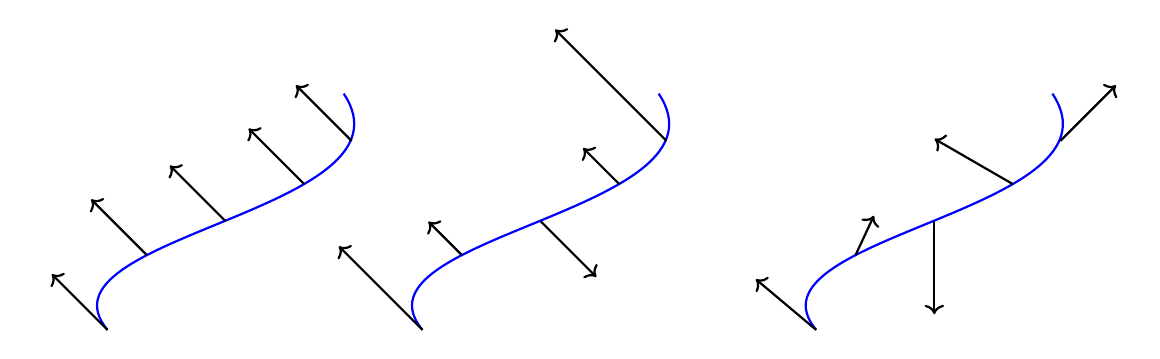
\begin{tikzpicture}
	\draw[thick, blue] (-4,0) .. controls (-5,1.2) and (0,1.5) .. (-1,3);
	\draw[thick, blue] (0,0) .. controls (-1,1.2) and (4,1.5) .. (3,3);
	\draw[thick, blue] (5,0) .. controls (4,1.2) and (9,1.5) .. (8,3);
	%
	\draw[->, thick, rotate around={45: (-4,0)}] (-4,0) -- (-4,1);
	\draw[->, thick, rotate around={45: (-3.5,0.95)}] (-3.5,0.95) -- (-3.5,1.95);
	\draw[->, thick, rotate around={45:(-2.5,1.38)}] (-2.5,1.38) -- (-2.5,2.38);
	\draw[->, thick, rotate around={45:(-1.5,1.85)}] (-1.5,1.85) -- (-1.5,2.85);
	\draw[->, thick, rotate around={45:(-0.9,2.4)}] (-0.9,2.4) -- (-0.9,3.4);
	%
	\draw[->, thick, rotate around={45: (0,0)}] (0,0) -- (0,1.5);
	\draw[->, thick, rotate around={45: (0.5,0.95)}] (0.5,0.95) -- (0.5,1.55);
	\draw[->, thick, rotate around={45:(1.5,1.38)}] (1.5,1.38) -- (1.5,0.38);
	\draw[->, thick, rotate around={45:(2.5,1.85)}] (2.5,1.85) -- (2.5,2.5);
	\draw[->, thick, rotate around={45:(3.1,2.4)}] (3.1,2.4) -- (3.1,4.4);
	% 
	\draw[->, thick, rotate around={50: (5,0)}] (5,0) -- (5,1);
	\draw[->, thick, rotate around={-25: (5.5,0.95)}] (5.5,0.95) -- (5.5,1.5);
	\draw[->, thick] (6.5,1.38) -- (6.5,0.2);
	\draw[->, thick, rotate around={60:(7.5,1.85)}] (7.5,1.85) -- (7.5,3);
	\draw[->, thick, rotate around={-45:(8.1,2.4)}] (8.1,2.4) -- (8.1,3.4);
	\end{tikzpicture}
\end{center}
The left drawing is a parallely transported vector field, the middle drawing is a parallel vector field. For the middle drawing, it's important that the vector field vanishes in-between points when it points "up" vs. "down" because $\mu:\mathbb{R} \to \mathbb{R}$ is smooth. The right drawing is not even parallel.

\subsubsection{Autoparallelly Transported Curves}

\begin{definition}[Autoparallely Transported]
	smooth curve $\gamma : \mathbb{R} \to M$ \textbf{autoparallely transported} if 
	\begin{equation}
		\nabla_{v_{\gamma}} v_{\gamma} = 0
	\end{equation}
\end{definition}

\begin{definition}
	smooth curve $\gamma : \mathbb{R} \to M$ is autoparallel 
	\begin{equation}
		\nabla_{v_{\gamma}} v_{\gamma} = \mu v_{\gamma}
	\end{equation}
for some smooth $\mu:\mathbb{R}\to \mathbb{R}$
\end{definition}

For autoparallel, it means we move in the straightest line. We are not talking about the shortest line because we do not have a notion of distance.

Note that the straightest line might not actually look straight when "viewed from above." That is, if we embed the manifold into a higher dimensional one, and then just look at the curve, it might be curved. For example, on a sphere, a straight line traces out a portion of a circle around the sphere. This doesn't look straight in the (higher, Euclidean) embedding, but \emph{on the surface} of the sphere, it's the straightest line.

\begin{center}
	\begin{tikzpicture} 
	\draw[thick] (-2,-2) -- (-1.5,-1.5);
	\draw[thick] (-1.4,-1.4) -- (-0.9,-0.9);
	\draw[thick] (-0.8,-0.8) -- (-0.3,-0.3);
	\draw[thick] (-0.2,-0.2) -- (0.3,0.3);
	\draw[thick] (0.4,0.4) -- (0.9,0.9);
	\draw[thick] (1,1) -- (1.5,1.5);
	%
	\draw[thick] (2,-2) -- (2.5,-1.5);
	\draw[thick] (2.6,-1.4) -- (3,-1);
	\draw[thick] (3.1,-0.9) -- (3.3,-0.7);
	\draw[thick] (3.4,-0.6) -- (3.5,-0.5);
	\draw[thick] (3.6,-0.4) -- (3.8,-0.2);
	\draw[thick] (3.9,-0.1) -- (4.3,0.3);
	\draw[thick] (4.4,0.4) -- (4.9,0.9);
	\draw[thick] (5,1) -- (5.5,1.5);
	\end{tikzpicture}
\end{center}
Left is an autoparallely transported curve, and the right is just an autoparallel.

Consider 
\[
\begin{gathered}
	\dot{\gamma}(t) = v(\gamma(t)) = v^i(\gamma^1(t) \dots \gamma^n(t)) \frac{\partial}{\partial x^i} \in T_{\gamma(t)} U
\end{gathered}\]
Then
\[
\begin{gathered}
	\frac{d}{dt}\dot{\gamma}(t) = \frac{d}{dt} v^i(\gamma^1(t) \dots \gamma^n(t)) \frac{\partial}{\partial x^i} = \frac{d}{dt} v^i(x^1 \dots x^n ) \frac{\partial}{\partial x^i} = \frac{\partial v^i}{\partial x^j}(x) \dot{x}^j \frac{\partial}{\partial x^i} = \dot{\gamma}^j \frac{\partial \dot{\gamma}^i}{\partial x^j} \frac{\partial }{ \partial x^i}
\end{gathered}\]
So
\[
\begin{gathered}
	\nabla_{v_{\gamma}} v_{\gamma} = \nabla_{v^j \frac{\partial}{\partial x^j} } v^i \frac{\partial}{\partial x^i} = v^j \left[ \frac{\partial v^i}{\partial x^j} \frac{\partial}{\partial x^i} + v^i \Gamma^k_{\, ij} \frac{\partial }{\partial x^k} \right] = \ddot{\gamma}(t) + \dot{\gamma}^i \dot{\gamma}^j \Gamma^k_{\, ij} \frac{\partial}{\partial x^k} \text{ i.e. }
\end{gathered}\]

\begin{equation}
	\boxed{ \nabla_{v_{\gamma}} v_{\gamma} = \left( \ddot{\gamma}^k(t) + \dot{\gamma}^i \dot{\gamma}^j \Gamma^k_{\, \, ij} \right) \frac{\partial }{ \partial x^k}  }
\end{equation}
with $\Gamma^k_{\, \, ij} = \Gamma^k_{\, \, ij}(\gamma(t))$.

\subsubsection{Torsion}
cf. Lecture 8, Schuller (2015) \cite{Schul2015}

\begin{definition}[torsion]
	The \textbf{torsion} of a connection $\nabla$ is the $(1,2)$-\textbf{tensor field}
	\begin{equation}
		T(\omega,X,Y) := \omega( \nabla_X Y - \nabla_Y X - [X,Y])
	\end{equation}
where $[\cdot, \cdot] : \Gamma(TM) \times \Gamma(TM) \to \Gamma(TM)$ is the commutator on $\Gamma(TM)$, that yields a vector field, $[X, Y]$ defined by
\begin{equation}
	[X,Y]f:= X(Yf) - Y(Xf)
\end{equation}
\end{definition}

\begin{theorem}
$T$ is $C^{\infty}$-linear in each entry
\end{theorem}

\begin{proof}
	check 
	
	\[
	\begin{gathered}
		T(f\cdot \omega, X, Y) = f\cdot \omega(\dots) = fT(\omega, X, Y) \\
		T(\omega + \psi, X, Y) = \dots = T(\omega, X, Y) + T(\psi, X, Y) \\
		T(\omega, fX, Y) = \omega( \nabla_{fX} Y - \nabla_Y (fX) - [fX, Y]) = \\
		= \omega(f\nabla_X Y - (Yf)X - f\nabla_Y X - f[X,Y] + (Yf)X) = fT(\omega,X,Y)
	\end{gathered}
	\]
	since
	\[
	\begin{gathered} 
		[fX,Y] g = fX(Yg) - Y(fXg) = fX(Yg) - (Yf) (Xg) - fY(Xg) = \\
		= f\cdot [X,Y] g - (Yf) Xg = (f\cdot [X,Y] - (Yf)X) g
	\end{gathered} 
	\]
	
	\[
	T(\omega, X, Y) = -T(\omega, Y , X)  \quad \, \checkmark
	\]
\end{proof}

\begin{definition}
	An affine manifold $(M, \mathcal{O}, \mathcal{A}, \nabla)$ is called torsion-free if $T=0$. This can also be written as
	\begin{equation}
		\nabla_X Y - \nabla_Y X = [X,Y] \quad \, \forall \, X, Y \in \Gamma(TM)
	\end{equation}	
\end{definition}

In a chart 
\[
\begin{aligned}
	T^i_{ \, \, ab } := T\left(dx^i , \frac{ \partial }{ \partial x^a} , \frac{ \partial }{ \partial x^b}  \right) & = dx^i ( \dots ) \\ 
	& = \Gamma^i_{ \, \, ba} - \Gamma^i_{ \, \, ab} = -2 \Gamma^i_{ \, \, [ab] }
\end{aligned}
\]
since
\[
\begin{gathered}
	[\frac{ \partial }{ \partial x^a}, \frac{ \partial }{ \partial x^b}] = 0 \text{ and } \\
	\nabla_{\frac{ \partial }{ \partial x^a} } \frac{ \partial }{ \partial x^b} = \Gamma^k_{\, \, ba} \\
	\nabla_{\frac{ \partial }{ \partial x^b} } \frac{ \partial }{ \partial x^a} = \Gamma^k_{\, \, ab} 
\end{gathered}\]
So what this means is that if the torsion is $0$, i.e. $T = T^i_{\, \, ab} = 0$, then the \emph{anti-symmetric} part of the connection coefficients, i.e. Christoffel symbols, is zero, $\Gamma^k_{\, [ij]} = 0$. So the Christoffel symbols only have a symmetric part and is thus symmetric in indices $i, j$.

From now on, in these lectures, we only use torsion-free connections. 



Suppose $X = X^i \frac{\partial}{\partial x^i} \in \mathfrak{X}(M)$, $s = s^i e_i \in \Gamma(E)$,
\[
D_X s =X^j D_{\frac{\partial }{ \partial x^j} } s^i e_i = X^j \left( \frac{\partial s^i}{\partial x^j} e_i + s^i D_{\frac{\partial }{\partial x^j} } e_i \right) = X^j \left( \frac{\partial s^k}{\partial x^j } + s^i \Gamma^k_{\, ij} \right) e_k
\]

Consider $\Gamma^k_{\, ij}$ as an ($n\times n$) matrix valued 1-form on $U$ \, $\forall \, j = 1 \dots d$.

\begin{equation}
	\Gamma^k_{\, ij} \in \Gamma( \mathfrak{gl}(n, \mathbb{R}) \otimes \left. T^* M \right|_U)
\end{equation}
cf. Eq. (4.1.12), pp. 166, Jost (2017) \cite{Jost2017}.

Abstract this to
\[
D = d+A
\]
where $d$ is the exterior derivative and $A \in \Gamma( \mathfrak{gl}(n, \mathbb{R}) \otimes \left. T^* M \right|_U)$.

Given $a^j e_j$
\[
D(a^j e_j) = e_k \otimes (da^k) + A_j a \otimes dx^j
\]

where $d(a^k)(X) = (da^k)(X) = X(a^k) = X^j \frac{\partial a^k}{\partial x^j}$. 

Let $(U_{\alpha})_{\alpha \in A}$ be covering of $M$ by open sets which the bundle is trivial, with transition maps
\[
\varphi_{\beta \alpha} : U_{\alpha} \cap U_{\beta} \to GL(n;\mathbb{R})
\]

Let section $s$ be represented by $s_{\alpha}$ on $U_{\alpha}$.

Thus,
\[
s_{\beta} = \varphi_{\beta \alpha} s_{\alpha} \text{ on } U_{\alpha} \cap U_{\beta}
\]

But then
\[
\begin{gathered}
	\varphi_{\beta \alpha} (d+A_{\alpha}) s_{\alpha} = (d+A_{\beta}) s_{\beta} \text{ on } U_{\alpha} \cap U_{\beta} \\
	\begin{gathered}
		\varphi_{\beta \alpha} ds_{\alpha} + \varphi_{\beta \alpha} A_{\alpha} s_{\alpha} = d\varphi_{\beta \alpha} s_{\alpha} + A_{\beta} \varphi_{\beta \alpha} s_{\alpha} \\
		A_{\alpha} s_{\alpha} = -ds_{\alpha} + \varphi^{-1}_{\beta \alpha} d\varphi_{\beta \alpha} s_{\alpha} + \varphi^{-1}_{\beta \alpha} A_{\beta} \varphi_{\beta \alpha} s_{\alpha}
	\end{gathered}
\end{gathered}
\]

\subsection{Curvature}

cf. Lecture 8, Schuller (2015) \cite{Schul2015}.

\begin{definition}[Riemann Curvature]
	The \textbf{Riemann curvature} of a connection $\nabla$ is the $(1,3)$-tensor field
	\begin{equation}
		\text{Riem}(\omega,Z,X,Y) := \omega( \nabla_X \nabla_Y Z - \nabla_Y \nabla_X Z - \nabla_{[X,Y]} Z)
	\end{equation}
\end{definition}

\begin{definition}[Ricci Curvature]
	Let Riem be the Riemann curvature tensor of connection $\nabla$. \\
	Define the Ricci curvature tensor as $(0, 2)$-tensor field
	\begin{equation}
		\text{Ric}(X, Y) := \text{Riem}(f^k, Y, X, e_k)
	\end{equation}
where $f^l(e_m) = \delta^l_{\, \, m}$

In terms of components, the Ricci curvature tensor is given by
\begin{equation}
	\text{Ric}_{ab} = \text{Riem}^m_{\, \, amb}
\end{equation}
\end{definition}

\begin{theorem}
	Riem is $C^{\infty}$-linear in each slot.
\end{theorem}

\begin{proof}
\[
\begin{gathered}
	\begin{aligned}
		\text{ since } & \text{Riem}(\omega, Z, X, Y) = \omega (\nabla_X \nabla_Y Z - \nabla_Y \nabla_X Z - \nabla_{[X,Y]} Z) \\
		& \text{Riem}(f\omega, Z, X, Y) = f\omega (\nabla_X \nabla_Y Z - \nabla_Y \nabla_X Z - \nabla_{[X,Y]} Z) = f\text{Riem}(\omega, Z, X, Y) \\
		& \text{Riem}(\omega + \sigma, Z, X, Y) = (\omega + \sigma) (\nabla_X \nabla_Y Z - \nabla_Y \nabla_X Z - \nabla_{[X,Y]} Z) = \text{Riem}(\omega, Z, X, Y) + \text{Riem}(\sigma, Z, X, Y) 
	\end{aligned} 
\end{gathered}\]
\[
\begin{gathered}
	\text{Riem}(\omega, Z, fX, Y) = \omega (f\nabla_X \nabla_Y Z - Y(f) \nabla_X Z - f\nabla_Y \nabla_X Z -  \nabla_{f[X,Y] - (Yf)X} Z ) = \\
	= \omega (f\nabla_X \nabla_Y Z - Y(f) \nabla_X Z - f\nabla_Y \nabla_X Z - f \nabla_{[X, Y]}Z + (Yf)\nabla_X Z) = f\text{Riem}(\omega, Z, X, Y) 
\end{gathered}\]
where the second and last term cancel each other out in the second to last expression.

\end{proof}

The Riemann curvature tensor Riem is antisymmetric in its last 2 entries. This is because

\[
\begin{gathered}
	\text{Riem}(\omega, Z, Y, X) = \omega(\nabla_Y \nabla_X Z - \nabla_X \nabla_Y Z - \nabla_{[Y,X]} Z) = -\omega(\nabla_X \nabla_Y Z - \nabla_Y \nabla_X Z + \nabla_{-[X,Y]} Z ) = \\
	= -\text{Riem}(\omega, Z, X, Y)
\end{gathered}
\]
since $\nabla_{-[X,Y]}Z = -\nabla_{[X,Y]}Z$

Therefore, Riem has $d^3 (d-1)/2$ independent components. This is because $d^4$ is the total number of components (there are 4 indices, each index running from 1 to d) if the indices are completely independent of each other. 

Since two entries are antisymmetric, imagine a $dxd$ matrix with only the entries in the "top half triangle" being independent. It excludes the diagonal entries (they'd be all 0). There are $\frac{d(d-1)}{2}$ entries. For each of those antisymmetric entries, there are still $d^2$ ways to choose the other 2 entries of the Riem. Thus, the number of independent components are
\[
\begin{gathered}
	d^4 = \left( \frac{d(d-1)}{2} \right) d^2 = d^4 - \frac{ (d^2 - d)d^2}{2} = d^4 - \frac{d^4- d^3}{2} = d^3(d-1)/2
\end{gathered}
\]

\part{Holonomy}

\begin{definition}[Conlon, 10.1.2] If $X,Y\in \mathfrak{X}(M)$, $M\subset \mathbb{R}^m$, \textbf{Levi-Civita connection} on $M\subset \mathbb{R}^m$
	\begin{equation}
	\begin{aligned}
	& \nabla : \mathfrak{X}(M) : \mathfrak{X}(M) \to \mathfrak{X}(M) \\
	\nabla_XY := p(D_XY)
	\end{aligned}
	\end{equation}
	with 
	\[
	D_XY := \sum_{j=1}^m X(Y^j) \frac{ \partial }{ \partial x^j} = \sum_{i,j=1}^m X^i \frac{ \partial Y^j}{ \partial x^i} \frac{ \partial }{ \partial x^j} \qquad \,  \begin{aligned} & \quad \\ 
		& \forall \, X=\sum_{i=1}^m X^i \frac{ \partial }{ \partial x^i},  \\
		& \forall \, Y=\sum_{i=1}^m Y^i \frac{\partial }{ \partial x^i } \end{aligned}
	\]
\end{definition}

\[
\begin{aligned}
	& \nabla_{fX}Y = f(D_{fX}Y) = p(fD_XY) = fpD_XY = f\nabla_XY \\ 
	&  \nabla_X fY = p(D_XfY) = p \left( \sum_{i,j=1}^m \left( X^i f\frac{ \partial Y^j}{ dx^i } + X^i Y^j \frac{ \partial f}{ \partial x^i} \right) \frac{ \partial }{ \partial x^j} \right) = f\nabla_X Y + p \sum_{j=1}^m X(f) Y^j \frac{ \partial }{ \partial x^j} = f\nabla_XY + X(f) p(Y)
\end{aligned}
\]


\begin{definition}[Conlon, 10.1.4; Christoffel symbols] 
\begin{equation}
\begin{gathered}
	\nabla_{\frac{ \partial }{ \partial x^i} \frac{ \partial }{ \partial x^j} = \Gamma^k_{ij} \frac{ \partial }{ \partial x^k} \qquad \, \text{ (Conlon's notation) }  }   \\
	\nabla_{\frac{ \partial }{ \partial x^j} \frac{ \partial }{ \partial x^i} = \Gamma^k_{ij} \frac{ \partial }{ \partial x^k} \qquad \, \text{ (F. Schuller's notation) }  }
\end{gathered}
\end{equation}
\end{definition}





\begin{definition}[torsion]
\begin{equation}
\begin{aligned}
	& T:\mathfrak{X}(M) \in \mathfrak{X}(M) \to \mathfrak{X}(M) \\ 
	& T(X,Y) = \nabla_XY - \nabla_Y X - [X,Y] 
\end{aligned}
\end{equation}
If $T=0$, $\nabla$ torsion-free or symmetric.  
\end{definition}
\[
\begin{gathered}
T(fX,Y) = f\nabla_XY - (f\nabla_Y X + Y(f)X) - \lbrace (fXY - (Y(f)X + fYX) \rbrace = fT(X,Y) \\ 
T(X,fY) = f\nabla_XY + X(f)Y - f\nabla_Y X   - \lbrace ( ( X(f) Y +fXY) -  fYX \rbrace = fT(X,Y)  
\end{gathered}
\]
Thus, $T(X,Y)$ $C^{\infty}(M)$-bilinear.  

$T\in \tau_1^2 (M)$.  

$T(v,w) \in T_xM$ defined, $\forall \, v,w \in T_xM$, $\forall \, x\in M$.

Thus, torsion is a \textbf{tensor}.

\exercisehead{10.1.7 Conlon (2008)\cite{Conl2008} }.  

If $T(X,Y)=0$,
\[
T(e_i,e_j) = \Gamma^k_{ji} e_k - \Gamma^k_{ij} e_k - 0 = 0 \Longrightarrow \Gamma_{ji}^k = \Gamma^k_{ij}
\]

If $\Gamma^k_{ij} = \Gamma^k_{ji}$, $T(e_i,e_j)=0$.  

\exercisehead{10.1.8, Conlon (2008)\cite{Conl2008}} 

If $M\subset \mathbb{R}^m$ smoothly embedded submanifold,  
$\forall \, \frac{ \partial }{ \partial x^j}, \frac{ \partial }{ \partial x^i} \in T_xM$, spanning $T_xM$, consider $\frac{ \partial }{ \partial x^j} = X^k_j \frac{ \partial }{ \partial \widetilde{x}^k}$, $\frac{ \partial }{ \partial x^i} = X_i^k(\widetilde{x}) \frac{ \partial }{ \partial \widetilde{x}^k}$  

\[
\begin{gathered}
	\nabla_{\frac{\partial }{ \partial x^j} } \frac{ \partial }{ \partial x^i} = p D_{ X^k_j \frac{ \partial }{ \partial \widetilde{x}^k } } X^l_i \frac{ \partial }{ \partial \widetilde{x}^l } = p \left( X^k_j \frac{ \partial X^l_i}{  \partial \widetilde{x}^k } \frac{ \partial }{ \partial \widetilde{x}^l } \right) =   X^k_j  p \left( \frac{ \partial X^l_i}{  \partial \widetilde{x}^k } \frac{ \partial }{ \partial \widetilde{x}^l } \right)  \\ 
	\nabla_{\frac{\partial }{ \partial x^i} } \frac{ \partial }{ \partial x^j} =  X^k_i p \left(  \frac{ \partial X^l_j }{ \partial \widetilde{x}^k }   \frac{ \partial }{ \partial \widetilde{x}^l  } \right) 
\end{gathered}
\]









If $X\in \mathfrak{X}(M)$, smooth $s:[a,b]\to M$, 

then $\forall \, s(t)$, 
\[
X'_{s(t)} = \nabla_{\dot{s}(t)} X \in T_{s(t)}M
\]
In fact, it's often natural to consider fields $X_{s(t)}$ along $s$, parametrized by parameter $t$, allowing
\[
X_{s(t_1)} \neq X_{s(t_2)}
\]
each of $s(t_1)=s(t_2)$.  

\begin{definition}[10.1.9] Let smooth $s:[a,b] \to M$.  

Vector field along $s$ is smooth $v:[a,b]\to TM$ s.t. 
\[
\begin{tikzpicture}
  \matrix (m) [matrix of math nodes, row sep=7.8em, column sep=12.8em, minimum width=5.2em]
  {
   &  TM  \\ 
	\left[ a,b \right] & M \\ 
};
  \path[|->]
  (m-2-1) edge node [above] {$ v $} (m-1-2)
edge node [above] {$s$} (m-2-2)
  (m-1-2) edge node [left] {$ \pi $} (m-2-2)
  ;
\end{tikzpicture}  
\]
commutes.

Note that $v\in \mathfrak{X}(s) \subset \mathfrak{X}(M)$
\end{definition}

e.g. $(Y|s)(t) = Y_{s(t)}$, restriction of $Y\in \mathfrak{X}(M) $ to $s$.  

e.g. $\dot{s}(t) \in \mathfrak{X}(M)$.  

$\forall \, v,w \in \mathfrak{X}(s)$, $v+w \in \mathfrak{X}(s)$, 
\[
\begin{gathered}
	(fv+gv)(t) := (f(s(t)) + g(s(t)) )v(t) = f(s(t)) v(t) + g(s(t)) v(t) = (f+g)v(t)
\end{gathered}
\]
Likewise, 
\[
f(v+w) = fv+fw
\]
$\mathfrak{X}(s)$ is a real vector space and $C^{\infty}[a,b]$-module.  

\begin{definition}[10.1.10]
Let conection $\nabla$ on $M$.  

\textbf{Associated covariant derivative} is operator 
\[
\frac{\nabla}{dt} \mathfrak{X}(s) \to \mathfrak{X}(s)
\]
$\forall \, $ smooth $s$ on $M$, s.t. 
\begin{enumerate}
\item $\frac{\nabla}{dt}$ $\mathbb{R}$-linear 
\item $\left( \frac{\nabla}{dt} \right)(fv) = \frac{df}{dt} v+ f\frac{\nabla}{dt} v$, $\forall \, f \in C^{\infty}[a,b]$, $\forall \, v\in \mathfrak{X}(s)$  
\item If $Y\in \mathfrak{X}(M)$, then
\[
\frac{\nabla}{dt} (Y|s)(t) = \nabla_{ \dot{s}(t)}Y \in T_{s(t)} M, \quad \, a\leq t \leq b
\]
\end{enumerate}
\end{definition}












\begin{theorem}[Conlon Thm. 10.1.11\cite{Conl2008} ]
	$\forall \, $ connection $\nabla$ on $M$, $\exists \, !$ \, associated covariant derivative $\frac{ \nabla }{dt}$
\end{theorem}

\begin{proof}
	Consider arbitrary coordinate chart $(U,x^1 \dots x^n)$.  
	
	Consider smooth curve $s:[a,b]\to U$.  
	
	Let $v\in \mathfrak{X}(s)$, $v(t) = v^i(t) \frac{ \partial }{ \partial x^i}$; $\dot{s}(t) = s^j \frac{ \partial }{ \partial x^j}$.  
	\[
	\begin{gathered}
	\frac{ \nabla v}{ dt} = \frac{dv^i(t) }{dt}\frac{ \partial }{ \partial x^i} + v^i(t) \frac{ \nabla}{dt} \frac{ \partial }{ \partial x^i} = \frac{ d v^i }{dt}	\frac{ \partial }{ \partial x^i} + v^i \nabla_{ \dot{s}(t) } \frac{ \partial }{ \partial x^i } = \dot{v}^i \frac{ \partial }{ \partial x^i } + v^i\dot{s}^j \Gamma^k_{ij} \frac{ \partial }{ \partial x^k} = \left( \dot{v}^k + v^i \dot{s}^j \Gamma^k_{ij} \right)\frac{ \partial }{ \partial x^k} \end{gathered}
	\]
	This is an explicit, local formula in terms of connection, proving uniqueness.  
	
	Existence: $\forall \, $ coordinate chart $(U,x^1\dots x^n)$, $\left( \dot{v}^k + v^i \dot{s}^j \Gamma_{ij}^k \right) \frac{ \partial }{ \partial x^k } =: \frac{ \nabla v}{dt}$.  
	
	\[
	\begin{gathered}
	\frac{\nabla}{dt}(fv) = \dot{f}v^k + f\dot{v}^k + fv^i \dot{s}^j = \dot{f}v + f\frac{ \nabla v}{dt}
	\end{gathered}
	\]
If $f$ constant, then $\frac{\nabla}{dt}$ is $\mathbb{R}$-linear.  	

\end{proof}

\begin{definition}[10.1.12 Conlon (2008)\cite{Conl2008}]
	Let $(M,\nabla)$.  Let $v\in\mathfrak{X}(s)$ for smooth $s:[a,b] \to M$.  

If $\frac{\nabla v}{dt} \equiv 0$ on $s$, then $v$ is \textbf{parallel } along $s$.  
\end{definition}

\begin{theorem}[10.1.13] 
Let $(M,\nabla)$, smooth $s:[a,b]\to M$, $c\in [a,b]$, $v_0 \in T_{s(c)}M$.  

Then $\exists \, !$ parallel field $v\in \mathfrak{X}(s)$ s.t. $v(c) = v_0$.  

$v$ parallel transport along $s$.  
\end{theorem}
\begin{proof}
	\[
\begin{aligned}
	& \dot{s}(t) = \dot{s}^j(t) e_j \\ 
	&  v(t) = v^i(t) e_i  \\
& v_0 = a^i e_i
\end{aligned}
\]
\[
0 = \left( \frac{dv^k}{dt}(t) + v^i(t) \dot{s}^j(t) \Gamma^k_{ij}(s(t)) \right) e_k
\]
or equivalently
\begin{equation}
	\frac{dv^k}{dt} = - v^i \dot{s}^j \Gamma^k_{ij} , \qquad \, 1\leq k \leq n \qquad \, (10.1)
\end{equation}
with initial conditions $v^k(c) = a^k$, $1\leq k \leq n$.  

By existence and uniqueness of solutions of O.D.E.  

$\exists \, \epsilon > 0$ s.t. $\exists \, !$ solutions $v^k(t)$.  For $c-\epsilon < t < c+\epsilon$.  

In fact, these ODEs being linear in $v^k$,  by ODE theory (Appendix C, Thm. C.4.1).  

$\nexists \, $ restriction on $\epsilon$, so $\exists \, ! \, v^k(t)$ \, $\forall \, t \in [a,b]$, $1\leq k \leq n$  

\end{proof}




\subsection{Principal bundle, vector bundle case for parallel transport}  

Recall the 2 different forms or viewpoints for Lie-algebra valued 1-forms, or vector-valued 1-forms, or sections of 1-form-valued endomorphisms:
\[
\omega^k_{ \,\, i\mu} dx^{\mu} \equiv \omega^k_{\,\,i} \in \Omega^1(M,\mathfrak{gl}(n,\mathbb{F})) = \Gamma(\mathfrak{gl}(n,\mathbb{R} \otimes \left. T^* M \right|_U ) )
\] 
for $\begin{aligned} & \quad \\
	& i,k = 1\dots n =\text{dim}E \\ 
	& \mu = 1\dots d =\text{dim}E \end{aligned}$.  

Now
\[
D_X\mu = X^{\mu} D_{\frac{\partial }{ \partial x^{\mu}}}\mu = X^{\mu} \left[ \left( \frac{ \partial }{ \partial x^{\mu}} \mu^k \right) e_k + \mu^i \omega^k_{ \,\, i\mu} e_k \right] = \left( X(\mu^k) + \mu^i \omega^k_{ \,\, i}(X) \right) e_k = \left( d\mu^k(X) + \mu^i \omega^k_{ \,\, i}(X) \right) e_k
\]
So then define 
\begin{equation}
	\begin{aligned}
		& D: \Gamma(E) \to \Gamma(E) \otimes \Gamma(T^*M) \\
	& D\mu  = D(\mu^i e_i) = e_k ( d\mu^k +\mu^i \omega^k_{ \,\, i}) \equiv (d+A)\mu
	\end{aligned}
\end{equation}

Also, $D$ can be defined for this case:
\[
D: \Gamma (\text{End}(E)) \to \Gamma(\text{End}E) \otimes \Gamma(T^*M)
\]
Let $\sigma = \sigma^i_{ \,\, j} e_i \otimes e^j \in \Gamma(\text{End}(E))$

\begin{equation}
\begin{gathered}
	D\sigma = D(\sigma^i_{ \,\, j} e_i ) \otimes e^j + \sigma^i_{ \,\, j} e_i \otimes D^* e^j = \left( d\sigma^k_{ \,\, j} + \sigma^i A^k_{ \,\, i} \right) e_k \otimes e^j + \sigma^i_{ \,\, j} e_i \otimes (A^*)_k^{ \,\, j} e^k = \\
	= (d\sigma^k_{ \,\, j} + \sigma^i_{ \,\, j} A^k_{ \,\, i} ) e_k \otimes e^j + \sigma^k_{ \,\, i} e_j \otimes (- A^i_{ \, \, j}) e^j = (d\sigma^k_{ \,\, j} + [A,\sigma]^k_{ \,\, j}) e_k\otimes e^j
\end{gathered}
\end{equation}
cf. Def. 4.1.4 of Jost (2017) \cite{Jost2017}, pp. 138.  

For $\mu \in \Gamma(E)$, smooth $s:[a,b] \to M$, $X(t) = \dot{s}(t)$,
\begin{equation}
D_{\dot{s}(t)}\mu = \dot{s}^{\mu}D_{\frac{ \partial }{ \partial x^{\mu}} } \mu = \dot{s}^{\mu} \left[ \frac{ \partial \mu^k }{ \partial x^{\mu}} e_k + \mu^i \omega^k_{ \, \, i\mu} e_k \right] = \left[ \dot{s}^{\mu} \frac{ \partial \mu^k}{ \partial x^{\mu} } + \dot{s}^{\mu} \mu^i \omega^k_{ \,\, i \mu} \right] e_k =\frac{d}{dt} \mu(s(t)) + \mu^i \dot{s}^{\mu} \omega^k_{ \,\, i \mu} e_k
\end{equation}

Let $D_{\dot{s}(t)}\mu=0$.  Then, 
\begin{equation}
\frac{d}{dt} \mu(s(t)) = -\mu^i \dot{s}^{\mu}\omega^k_{ \,\, i\mu} e_k
\end{equation}


Recall, given vector bundle $E\xrightarrow{ \pi} N$, given $\varphi : M\to N$, then pullback 
\begin{equation}
	\varphi^* E \to M
\end{equation}
i.e. 

\[
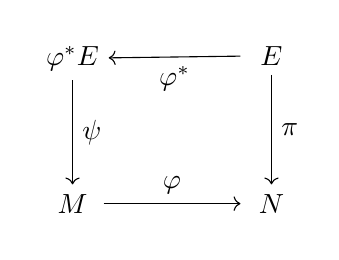
\begin{tikzpicture}
\matrix (m) [matrix of math nodes, row sep=3.8em, column sep=4.8em, minimum width=2.2em]
{
	\varphi^* E &  E  \\
	M  &  N  \\
};
\path[->]
(m-1-2) edge node [auto] {$ \varphi^*  $} (m-1-1)
edge node [auto] {$ \pi $} (m-2-2)
(m-2-1) edge node [auto]  {$  \varphi $} (m-2-2)
(m-1-1) edge node [auto] {$\psi$} (m-2-1)
;
\end{tikzpicture}
\qquad \, 
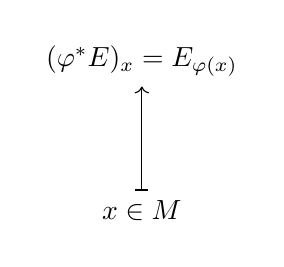
\begin{tikzpicture}
\matrix (m) [matrix of math nodes, row sep=3.8em, column sep=4.8em, minimum width=2.2em]
{
	(\varphi^* E)_x = E_{\varphi(x)}  \\
	 x\in M \\
};
 \path[|->]
	(m-2-1) edge node [auto] {$$} (m-1-1)
;
\end{tikzpicture}
\]
i.e. if $s\in \Gamma(E)$, 
\[
\varphi^* s = s \circ \varphi \in \Gamma( \varphi^* E)
\]
Thus,
\[
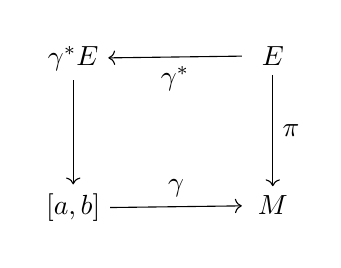
\begin{tikzpicture}
\matrix (m) [matrix of math nodes, row sep=3.8em, column sep=4.8em, minimum width=2.2em]
{
	\gamma^* E &  E  \\
	\left[a,b\right]  &  M  \\
};
\path[->]
(m-1-2) edge node [auto] {$ \gamma^*  $} (m-1-1)
edge node [auto] {$ \pi $} (m-2-2)
(m-2-1) edge node [auto]  {$  \gamma $} (m-2-2)
(m-1-1) edge node [auto] {$ $} (m-2-1)
;
\end{tikzpicture}
\qquad \, 
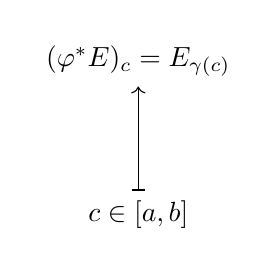
\begin{tikzpicture}
\matrix (m) [matrix of math nodes, row sep=3.8em, column sep=4.8em, minimum width=2.2em]
{
	(\varphi^* E)_c = E_{\gamma(c)}  \\
	 c\in  [a,b]\\
};
 \path[|->]
	(m-2-1) edge node [auto] {$$} (m-1-1)
;
\end{tikzpicture}
\]







For 
\[
\begin{gathered}
\dot{v}^k = -v^i \dot{s}^j \Gamma^k_{ \, \, ij}   \\
v^k(c) = v_0^k \qquad \, 1 \leq k \leq m
\end{gathered}
\]
\[
\dot{v} = -v^i \dot{s}^j \Gamma_{ij}
\]
\[
\begin{gathered}
\dot{ (v+w) } = -(v^i + w^i) \dot{s}^j \Gamma_{ij}
(v+w)(c) = v(c) + w(c) = v_0 + w_0 
\end{gathered}
\]
so $v+w\in \mathfrak{X}(s)$ is parallel transport of $v_0 + w_0$.  

Likewise, $\forall \, a \in \mathbb{F}$, $av \in \mathfrak{X}(s)$ is the parallel transport of $av_0$.  

\[
\dot{\mu}^k = - \mu^i \dot{s}^{\mu} \omega^k_{ \, \, i \mu} = -\mu^i \omega^k_{ \,\, i}(\dot{s}^{\mu})
\]


Suppose $\gamma^*E$ trivialized over $[a,b]$.  

Closed interval is contractible, so this is always possible.  

For chart $(U,\varphi)$, 
\[
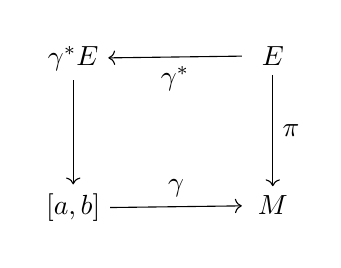
\begin{tikzpicture}
\matrix (m) [matrix of math nodes, row sep=3.8em, column sep=4.8em, minimum width=2.2em]
{
	\gamma^* E   &  E    \\
	\left[a,b\right]  &  M  \\
};
\path[->]
(m-1-2) edge node [auto] {$ \gamma^*  $} (m-1-1)
edge node [auto] {$ \pi $} (m-2-2)
(m-2-1) edge node [auto]  {$  \gamma $} (m-2-2)
(m-1-1) edge node [auto] {$ $} (m-2-1)
;
\end{tikzpicture} \qquad \, 
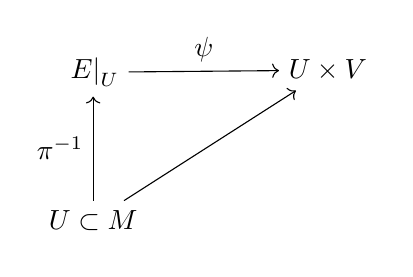
\begin{tikzpicture}
\matrix (m) [matrix of math nodes, row sep=3.8em, column sep=4.8em, minimum width=2.2em]
{
	\left. E \right|_U   &   U\times V  \\
	U \subset M    &    \\
};
\path[->]
(m-2-1) edge node [auto] {$ \pi^{-1}  $} (m-1-1)
edge node [auto] {$  $} (m-1-2)
(m-1-1) edge node [auto]  {$  \psi $} (m-1-2)
%(m-1-1) edge node [auto] {$ $} (m-2-1)
;
\end{tikzpicture}
\]
Consider 
\[
\begin{aligned}
& \varphi:[a,b]  \times V \to \gamma^* E \\ 
& \varphi(t,\cdot ) = \gamma^* \circ \psi^{-1}(\gamma(t), \cdot ) 
\end{aligned}
\]
$\forall \, \mu \in \Gamma( \left. E\right|_{x\in M} )$, \\ 
$\mu = \mu^i e_i$.  

$\varphi(t,e_i) = \epsilon_i$ is a basis for $\gamma^* E$.  

$\forall \, \sigma \in \Gamma(\gamma^*E)$,  
\[
\sigma  = \sigma^i \epsilon_i, \quad \, \sigma^i: [a,b] \to \mathbb{F}
\]
\[
\begin{gathered}
	\nabla_{ \frac{ \partial }{ \partial x^{\mu} } } \sigma = \frac{ \partial \sigma^k}{ \partial x^{\mu}  } \epsilon_k + \omega^k_{ \, \, j \mu } \sigma^j \epsilon_k = \left( \frac{ \partial \sigma ^k }{ \partial x^{\mu } } + \omega^k_{ \ , \, j \mu} \sigma^j  \right)  \epsilon_k \\ 
 \nabla \sigma = \epsilon_k \otimes ( d\sigma^k + \omega^k_{ \, \, j \mu} dx^{\mu} \sigma^j ) = \epsilon_k \otimes (d\sigma^k + \omega^k_{ \, \, j} \sigma^j  )  \\
 \nabla_{ \frac{d}{dt} } \sigma = \epsilon_k \otimes \left( \frac{d\sigma^k }{ dt } + \omega^k_{ \, \, j \mu } \dot{x}^{\mu} \sigma^j  \right)
\end{gathered}
\]
Now
\[
\frac{d}{dt} = \dot{x}^{\nu} \frac{ \partial }{ \partial x^{\nu } }
\]
Then $\sigma$ parallel along $\gamma$ if 
\[
\frac{ d\sigma^k}{ dt} + \omega^k_{ \, \, j\mu} \dot{x}^{\mu} \sigma^j = 0 
\]
\begin{definition}[3.1.4 \cite{ClSa2012}]  Parallel transport along $\gamma$ is 
\begin{equation}
\begin{aligned}
	& P_{\gamma} : E_{\gamma(a)} \to E_{\gamma(b)} \\ 
	& P_{\gamma}(v) \mapsto \sigma(b)
\end{aligned}
\end{equation}
where $\sigma \in \Gamma(\gamma^*E)$, $\sigma$ unique and s.t. $\sigma(a)=v$.  
\end{definition}







\begin{lemma}[10.1.16\cite{Conl2008}]
	holonomy 
	\[
	h_s:T_xM \to T_{x_0}M
	\]
	if $\nabla$ around piecewise smooth loop $s$ is a linear transformation.  
\end{lemma}






\begin{lemma}[10.1.18 Conlon (2008)\cite{Conl2008}] 
	Let piecewise smooth loop $s:[a,b] \to M$ at $x_0$.  

Let weak reparametrization $\widetilde{s} = s\circ r: [c,d] \to M$.  

If reparametrization is orientation-preserving, then $h_{\widetilde{s}} = h_s$, \\
If reparametrization is orientation-reversing, then $h_{\widetilde{s}} = h^{-1}_s$, 

\end{lemma}
\begin{proof}
	Without loss of generality,  assume smooth $s,r$
\[
\begin{aligned}
	& \widetilde{s}(\tau) = s(r(\tau)) \\ 
	& \widetilde{v}(\tau) = v(r(\tau))
\end{aligned}
\]
\[
\begin{aligned}
	& \widetilde{u}^j(\tau) = \frac{dt}{d\tau}(\tau) u^j(r(\tau)) \\ 
	& \frac{d\widetilde{v}^k}{d\tau} (\tau) = \frac{dr}{d\tau}(\tau) \frac{dv^k}{dt}(r(\tau)) \\ 
	& \frac{d\widetilde{v}^k }{ d\tau} = -\widetilde{v}^i \widetilde{u}^j \Gamma^k_{ij} 
\end{aligned}
\]
since \[
\begin{gathered}
	\frac{dv^k}{dt} = -v^i u^j \Gamma^k_{ij} ; \qquad \, 1\leq k \leq n \\ 
v^k(c) = a^k; \qquad \, 1\leq k \leq a 
\end{gathered}
\]
\[
\frac{dr}{d\tau} \frac{dv^k}{ dt} = -v^i \frac{dr}{d\tau} u^j \Gamma^k_{ \, \, ij} = \frac{d\widetilde{v}^k}{d\tau} = -\widetilde{v}^i \widetilde{u}^j \Gamma^k_{ \, \, ij}
\]
Thus, if $r(c) = a$, $r(d)=b$
\[
h_{\widetilde{s}}(v_0) = \widetilde{v}(d) = v(b) = h_s(v_0)
\]
If $r(c)=a$, $r(d)=b$, then 
\[
\widetilde{v}(c) = v(b) = h_s(v_0)
\]
and 
\[
h_{\widetilde{s}}(h_s(v_0)) = h_{\widetilde{s}}(v(b)) = \widetilde{v}(d) = v(a) = v_0
\]
At this point, I will switch to my notation because it clarified to me, at least, what was going on, in that a holonomy $h_s$ is \emph{invariant} under orientation-preserving reparametrization, and its inverse is well-defined.  

For $\widetilde{s} = s\circ t:[c,d] \to M$, \\
piecewise smooth $t$ is reparametrized, i.e. 
\begin{equation}
	t:[c,d] \to [a,b]
\end{equation}  
Now, 
\[
\begin{gathered}
	\frac{d}{d\tau}\widetilde{s}(\tau) = \frac{d}{d\tau} \widetilde{s}(t(\tau)) = \dot{s}(t) \frac{dt}{d\tau}(\tau) \equiv \dot{s} \frac{dt}{d\tau} \\ 
v^k(t) = v^k(t(\tau)) = v^k(\tau) \\ 
 \frac{dv^k}{d\tau}(t(\tau) ) = \frac{dv^k}{dt} \frac{dt}{ d\tau } = \frac{dt}{d\tau}(-v^i( \tau) \dot{s}^j(t) \Gamma^k_{ \,\, ij} ) = -v^i(\tau) \frac{d\widetilde{s}^j }{ d\tau} \Gamma^k_{ \, \, ij} 
\end{gathered}
\]
Consider 
\[
h_s(v_0) = v(b)
\]
If $\begin{aligned} & \quad \\ 
	& t(c) = a \\ 
	& t(d)=b \end{aligned}$, 
\[
h_{\widetilde{s}}(v_0) = \widetilde{v}(d) = v(t(d)) = v(b) = h_s(v_0)
\]
If $\begin{aligned} & \quad \\ 
	& t(c) = b \\ 
	& t(d)=a \end{aligned}$, 
\[
\begin{gathered}
h_{\widetilde{s}}(h_s(v_0) )  = h_{\widetilde{s}}( v(b)) = h_{\widetilde{s}}(v(t(c))) = h_{\widetilde{s}}(\widetilde{v}(c)) = \\
	= \widetilde{v}(d) = v(t(d)) = v(a) = v_0
\end{gathered}
\]
Thus, 
\[
\boxed{ h_{\widetilde{s}}= h_s^{-1} }
\]


\end{proof}

I am working through Conlon (2008) \cite{Conl2008} , Clarke and Santoro (2012) \cite{ClSa2012}, and Schreiber and Waldorf (2007)\cite{ScWa2007}, concurrently, for holonomy.  

\section{Path Groupoid of a smooth manifold; generalization of paths}
cf. Schreiber and Waldorf (2007)\cite{ScWa2007}.  

\begin{definition}[path]
	\textbf{path} is a smooth map $\gamma:[0,1] \to M$, between 2 pts. $x,y \in M$, \\
	which has a sitting instant; i.e. number $0 < \epsilon < \frac{1}{2}$ s.t. 
	\begin{equation}
	\gamma(t) = \begin{cases} x & \text{ for } 0 \leq t < \epsilon \\
	y & \text{ for } 1 - \epsilon < t \leq 1 \end{cases}
	\end{equation}

Denote the set of such paths by $PM$, 
\begin{equation}
PM \equiv \lbrace \gamma \in \Gamma(M) | \text{ smooth } \gamma : [0,1] \to M \text{ s.t. } \exists \, 0 < \epsilon < \frac{1}{2} \text{ s.t. } \begin{cases} x & \text{ for } 0 \leq t < \epsilon \\
y & \text{ for } 1 - \epsilon < t \leq 1 \end{cases} \rbrace
\end{equation}
\end{definition}
cf. Def. 2.1. of Schreiber and Waldorf (2007)\cite{ScWa2007}  

Define \emph{composition}: \\
Given paths $\gamma_1, \gamma_2$; $\begin{aligned} & \qquad \\ 
& \gamma_1(0) = x \\
& \gamma_1(1) = y \end{aligned}$, \, $\begin{aligned} & \qquad \\ 
& \gamma_2(0) = y \\
& \gamma_2(1) = z \end{aligned}$, \\
define composition to be path 
\begin{equation}
\begin{gathered}
\gamma_2 \circ \gamma_1 \\
(\gamma_2 \circ \gamma_1)(t) := \begin{cases} \gamma_1(2t) & \text{ for } 0 \leq t \leq \frac{1}{2} \\
\gamma_2(2t-1) & \text{ for } \frac{1}{2} \leq t \leq 1 \end{cases} 
\end{gathered}
\end{equation}

$\gamma_2 \circ \gamma_1$ smooth since $\gamma_1, \gamma_2$ both constant near gluing pt., due to sitting instants $\epsilon_1, \epsilon_2$, respectively. 

Define \emph{inverse}:
\begin{equation}
\begin{gathered}
\gamma^{-1} : [0,1] \to M \\
\gamma^{-1}(t) := \gamma(1-t)
\end{gathered}
\end{equation}
(so that $\gamma^{1}(t) =  \begin{cases} y & \text{ for } 1-\epsilon < 1-t \leq 1 \text{ or } 0 \leq t < \epsilon  \\
x & \text{ for } 0  \leq 1 - t < \epsilon \text{ or } 1 - \epsilon < t \leq 1 \end{cases}$)

\begin{definition}[thin homotopy equivalent]
2 paths $\gamma_1$, $\gamma_2$ s.t. $\begin{aligned} & \quad \\ & \gamma_1(0) = \gamma_2(0) = x \\
& \gamma_1(1) = \gamma_2(1) = y \end{aligned}$, $\gamma_1, \gamma_2$ are thin homotopy equivalent, \\
if $\exists \, $ smooth $h: [0,1] \times [0,1] \to M$ s.t. 
\begin{enumerate}
	\item $\exists \, 0 < \epsilon < \frac{1}{2} $ with 
	\begin{enumerate}
		\item $\begin{aligned} & \qquad \\
		& h(s,t) = x \text{ for } 0 \leq t < \epsilon \\
		& h(s,t) = y \text{ for } 1-\epsilon < t \leq  1 \end{aligned}$ 
		\item 		\item $\begin{aligned} & \qquad \\
		& h(s,t) = \gamma_1(t) \text{ for } 0 \leq s < \epsilon \\
		& h(s,t) = \gamma_2(t) \text{ for } 1-\epsilon < s \leq  1 \end{aligned}$
	\end{enumerate}
\item differential of $h$ has at most rank 1 everywhere, i.e. 
\begin{equation}
\text{rank}(\left. dh\right|_{(s,t)}) \leq 1 \qquad \, \forall \, (s,t) \in [0,1]\times [0,1]
\end{equation}
\end{enumerate}
\end{definition}
cf. Def. 2.2. of Schreiber and Waldorf (2007)\cite{ScWa2007}  

$\begin{aligned} & \qquad \\
& h(s,t) = \gamma_1(t) \text{ for } 0 \leq s < \epsilon \\
& h(s,t) = \gamma_2(t) \text{ for } 1-\epsilon < s \leq  1 \end{aligned}$ is the homotopy from $\gamma_1$ to $\gamma_2$, i.e. $\begin{aligned} & \quad \\ 
& h(0,t) = \gamma_1(t) \\
& h(1,t) = \gamma_2(t) \end{aligned}$  \\
and define an equivalence relation on $PM$.  

Note that for $h:[0,1] \times [0,1] \to M$, 
\[
\left. (Dh) \right|_{(s,t)} = \left[ \frac{ \partial h^i }{ \partial s} , \frac{\partial h^i }{ \partial t} \right]
\]


\begin{equation}
\begin{gathered}
P^1 M \equiv \text{ set of thin homotopy classes of paths, i.e. } \\ 
P^1 M = \lbrace [ \gamma] | \gamma_1 \in PM, \text{ if } \exists \, \text{ smooth } h:[0,1]\times [0,1] \to M \text{ s.t. } h \text{ thin homotopy of } \gamma_1 \text{ and } \gamma_2, \gamma_1 \sim \gamma_2 \rbrace
\end{gathered}
\end{equation}

$\text{pr}:PM \to P^1M$ is projection to classes.

Denote thin homotopy class of path $\gamma$, $\begin{aligned} & \qquad \\ 
& \gamma(0) = x \\
& \gamma(1) = y \end{aligned}$, by $\overline{\gamma}$, or $[\gamma]$.  

\subsection{Reparametrization of thin homotopies}

Let $\beta: [0,1] \to [0,1]$, $\begin{aligned} & \quad \\ 
& \beta(0) = 0 \\
& \beta(1) = 1 \end{aligned}$.  

Then $\forall \, $ path $\gamma$, $\begin{aligned} & \quad \\ 
& \gamma(0) = x \\
& \gamma(1) = y \end{aligned}$, $\gamma \circ \beta$ is also a path $\begin{aligned} & \quad \\ 
& \gamma\circ \beta(0) = x \\
& \gamma\circ \beta(1) = y \end{aligned}$ and 
\begin{equation}
h(s,t) := \gamma(t\beta(1-s) + \beta(t) \beta(s)
\end{equation}
defines a homotopy from $\gamma$ to $\gamma \circ \beta$.

\[
\gamma_1 \circ \gamma_2 \in PM \xmapsto{\text{pr}} [\gamma_1 \circ \gamma_2] = [\gamma_1][ \gamma_2] \in P^1M
\]

Composition of thin homotopy classes of paths obeys following rules:
\begin{lemma}\label{Eq:CompositionOfThinHomotopyClassesOfPaths}
$\forall$ path $\gamma$, $\begin{aligned} & \quad \\ 
& \gamma(0) = x \\
& \gamma(1) = y \end{aligned}$
\begin{enumerate}
	\item $\overline{\gamma} \circ \overline{\text{id}_x} = \overline{\gamma} = \overline{\text{id}_y} \circ \overline{\gamma} \equiv [\gamma]1_x = [\gamma] = 1_y [\gamma] $ 
	\item for paths $\gamma'$; $\begin{aligned} & \quad \\ 
		& \gamma'(0) = y \\
		& \gamma'(1) = z \end{aligned}$, \quad $\begin{aligned} & \quad \\ 
	& \gamma''(0) = z \\
& \gamma''(1) = w \end{aligned}$
\begin{equation}
(\overline{\gamma}'' \circ \overline{\gamma}') \circ \overline{\gamma} = \overline{\gamma}'' \circ (\overline{\gamma}' \circ \overline{\gamma}) \equiv ( [\gamma''][\gamma'])[\gamma] = [\gamma'']([\gamma'][\gamma])
\end{equation}
\item $\overline{\gamma} \circ \overline{\gamma}^{-1} = \overline{\text{id}_y}$ and $\overline{\gamma^{-1}} \circ \overline{\gamma} = \overline{\text{id}_x}$ $\equiv [\gamma] [\gamma^{-1}] = 1_y \text{ and } [\gamma^{-1}][\gamma] = 1_x$
\end{enumerate} 	
\end{lemma}
cf. Lemma 2.3. of Schreiber and Waldorf (2007)\cite{ScWa2007}  

\begin{definition}[path groupoid]
	$\forall \, $ smooth manifold $M$, \\
	consider category whose set of objects is $M$, \\
	whose set of morphisms is $P^1M$, where class $[\gamma]$, $\begin{aligned} & \qquad \\ 
	& [\gamma](0) = x \\
	& [\gamma](1) = y \end{aligned}$ is a morphism from $x$ to $y$ and \\
	composition $[\gamma_1 ][\gamma_2] = [\gamma_1 \circ \gamma_2] \in P^1M$  
	Lemma \ref{Eq:CompositionOfThinHomotopyClassesOfPaths} are axioms of a category, 3rd. property says $\forall \,$ morphism is invertible.  
	
	Hence, we've defined a groupoid, called \textbf{path groupoid} of $M$, $\mathcal{P}_1(M)$. 
\end{definition}

So 
\[
\begin{gathered}
\text{Obj}(\mathcal{P}_1(M)) = M \\
\text{Mor}(\mathcal{P}_1(M)) = P^1M
\end{gathered}
\]
$\forall \, $ smooth $f:M \to N$, denote functor $f_*$
\begin{equation}
f_* : \mathcal{P}_1(M) \to \mathcal{P}_1(N)
\end{equation}
with 
\[
\begin{gathered}
f_*(x) = f(x) \\
(f_*)([\gamma]) := [f\circ \gamma]
\end{gathered}
\]
If $\gamma \sim \gamma'$, for $f\circ \gamma$, $f\circ \gamma'$, \\
$f\circ h(s,t) $ with $\begin{aligned} & \quad \\ 
& f\circ h(0,t) = f\circ \gamma(t) \\
& f\circ h(1,t) = f\circ \gamma'(t) \end{aligned}$, \\
so $f\circ h$ is a thin homotopy between $f\circ \gamma$, $f\circ \gamma'$ and so $[f\circ \gamma]$ \emph{well-defined}.




\part{Complex Manifolds}

EY : 20170123 I don't see many good books on Complex Manifolds for physicists other than Nakahara's.  I will supplement this section on Complex Manifolds with external links to the notes of other courses that I found useful to myself.


\href{http://www.caramdir.at/uploads/math/piii-cm/complex-manifolds.pdf}{Complex Manifolds - Lecture Notes}
Koppensteiner (2010) \cite{Kopp2010}


\href{http://www.staff.science.uu.nl/~vando101/MRIlectures.pdf}{Lectures on Riemannian Geometry, Part II: Complex Manifolds by Stefan Vandoren}

Vandoren (2008) \cite{Vand2008}

\part{Jets, Jet bundles, $h$-principle, $h$-Prinzipien}

cf. Eliashberg and Misahchev (2002) \cite{ElMi2002}

cf. Ch. 1 Jets and Holonomy, Sec. 1.1 Maps and sections of Eliashberg and Misahchev (2002) \cite{ElMi2002}.  

Visualize $f:\mathbb{R}^n \to \mathbb{R}^q$ as graph $\Gamma_f \subset \mathbb{R}^n \times \mathbb{R}^q$.  

Consider this graph as image of $\begin{aligned} & \quad \\ 
	& \mathbb{R}^n \to \mathbb{R}^n \times \mathbb{R}^q \\
	& x \mapsto (x,f(x)) \end{aligned}$, i.e. 

$\begin{aligned} & \quad \\ 
	& \mathbb{R}^n \to \mathbb{R}^n \times \mathbb{R}^q \\
	& x \mapsto (x,f(x)) \end{aligned}$ is called section (by mathematicians), \\
is called \emph{field} or $\mathbb{R}^q$-valued field (by physicists).  

cf. Ch. 1 Jets and Holonomy, Sec. 1.2 Coordinate definition of jets of Eliashberg and Misahchev (2002) \cite{ElMi2002}.  

\begin{definition}[$r$-jet]
Given (smooth) $f: \mathbb{R}^n \to \mathbb{R}^q$, given $x\in \mathbb{R}^n$.  

$r$-jet of $f$ at $x$ - sequence of derivatives of $f$, up to order $r$, $\equiv$ 
\begin{equation}
J^r_f(x) = (f(x),f'(x) \dots f^{(r)}(x) )
\end{equation}
\end{definition}

$f^{(q)}$ consists of all partial derivatives $D^{\alpha}f$, $\alpha= (\alpha_1\dots \alpha_n)$, $|\alpha| = \alpha_1 + \dots + \alpha_n =s$, ordered lexicographically.  

e.g. $q=1$, \\
$f: \mathbb{R}^n \to \mathbb{R}$.   \\
1-jet of $f$ at $x = J_f^1(x) = (f(x), f^{(1)}(x))$.  
\[
f^{(1)}(x) = \lbrace D^{\alpha}f| \alpha = (\alpha_1 \dots \alpha_n), |\alpha| = \alpha_1  + \dots + \alpha_n  =1 \rbrace = \left( \frac{ \partial f}{ \partial x^1 }, \frac{ \partial f}{ \partial x^2 } , \dots \frac{ \partial f}{ \partial x^n } \right)
\]
Let $d_r = d(n,r) = $ number of all partial derivatives $D^{\alpha}$ of order $r$ of function $\mathbb{R}^n \to \mathbb{R}$.  

Consider $r$-jet $J^r_f(x)$ of map $f:\mathbb{R}^n\to \mathbb{R}^q$ as pt. of space $\mathbb{R}^q \times \mathbb{R}^{qd_1} \times \mathbb{R}^{qd_2} \times \dots \times \mathbb{R}^{qd_r} = \mathbb{R}^{q N_r}$, where $N_r = N(n,r) = 1 + d_1 + d_2 + \dots + d_r$, i.e. 
\[
J_f^r(x) = (f(x),f^{(1)}(x) , \dots f^{(r)}(x) ) \in \mathbb{R}^q \times \mathbb{R}^{qd_1} \times  \dots \times \mathbb{R}^{qd_r} = \mathbb{R}^{q N_r}
\]


\exercisehead{1}  

Given order $r$, consider $n$-tuple of (positive) integers $(r_1,r_2\dots r_n)$ s.t. $r_1 + r_2 + \dots + r_n = r$, and $r_k\geq 0$. \\
 Imagine $r_k = $ occupancy number, num ber of balls in $k$th cell.  $(r_1\dots r_n)$ describes a positive ocnfiguration of occupancy numbers, with indistinguishable balls; 2 distributions are distinguishable only if corresponding $n$-tuples $(r_1 \dots r_n)$ not identical.  

Represent balls by stars, and indicate $n$ cells by $n$ spaces between $n+1$ bars.  

With $n+1$ bars, $r$ stars, 2 bars are fixed. $n-1$ bars and $r$ stars to arrange linearly, so a total of $n-1+r$ objects to arrange.  $r$ stars indistinguishable amongst themselves, so choose $r$ out of $n-1+r$ to be stars.  
\begin{equation}
\Longrightarrow d_r = d(n,r)=\binom{n-1+r}{r}
\end{equation}

Use \emph{induction} (cf. \href{http://www.cs.columbia.edu/~cs4205/files/CM4.pdf}{Ch. 4 Binomial Coefficients}).  
\[
\begin{aligned}
	& N_0 = N(n,0) = \binom{n-1+0}{0} = 1 \\ 
	& N_1 = N(n,1) = 1+ \binom{n-1+1}{1} = 1 + n = \frac{ (n+1)!}{n! 1!}
\end{aligned}
\]
Induction step: 
\[
N_{r-1} = N(n,r-1) = \sum_{k=1}^{r-1} d_k + 1 = \binom{ n+r-1}{r-1}
\]
and so 
\[
\begin{gathered}
N_r = N(n,r) = \sum_{k=1}^r d_k + 1 = \sum_{k=1}^r \binom{n-1+k}{k} + 1 = \sum_{k=1}^{r-1} \binom{ n-1 +k}{k} + \binom{n-1+r}{r} + 1 = \\
	 =  \binom{n+r-1}{r-1} + \binom{n-1+r}{r} = \frac{ (n+r-1)! }{ (r-1)! n!} + \frac{ (n-1+r)! }{ r! (n-1)! } = \frac{ (n+r)!}{n!r!} = \binom{n+r}{r}
\end{gathered}
\]
\[
\begin{tikzpicture}
  \matrix (m) [matrix of math nodes, row sep=3.8em, column sep=4.8em, minimum width=2.2em]
  {
    \mathbb{R}^{qN_r} &  \\ 
    \mathbb{R}^n & \mathbb{R}^q \\ 
};
  \path[->]
  (m-2-1) edge node [auto] {$ J_f^r $} (m-1-1)
          edge node [auto] {$f $} (m-2-2)
  ;
\end{tikzpicture}   \quad \quad \, \begin{tikzpicture}
  \matrix (m) [matrix of math nodes, row sep=3.8em, column sep=4.8em, minimum width=2.2em]
  {
   J_f^r(x)  &  \\ 
    x & f(x) \\ 
};
  \path[|->]
  (m-2-1) edge node [auto] {$ J_f^r $} (m-1-1)
          edge node [auto] {$f $} (m-2-2)
  ;
\end{tikzpicture}  
\]

\begin{definition}[space of $r$-jets]
space of $r$-jects of maps $\mathbb{R}^n \to \mathbb{R}^q$ or space of $r$-jets of sections $\mathbb{R}^n \to \mathbb{R}^n \times \mathbb{R}^q \equiv $
\begin{equation}
J^r(\mathbb{R}^n, \mathbb{R}^q) = \mathbb{R}^n \times \mathbb{R}^{qN_r} \equiv \mathbb{R}^n \times \mathbb{R}^q \times \mathbb{R}^{qd_1} \times \mathbb{R}^{qd_2} \times \dots \times \mathbb{R}^{qd_r}
\end{equation}
e.g. $J^1(\mathbb{R}^n, \mathbb{R}^q) = \mathbb{R}^n \times \mathbb{R}^q \times M_{q\times n}$, where $M_{q\times n} = \mathbb{R}^{qn}$ is the space of $(q\times n)$-matrices.  
\end{definition}


\part{Morse Theory}

\section{Morse Theory introduction from a physicist}

I needed some physical motivation to understand Morse theory, and so I looked at Hori, et. al. \cite{Hori2003}.  

cf. pp. 43, Sec. 3.4 Morse Theory, from Ch. 3. Differential and Algebraic Topology of Hori, et. al. \cite{Hori2003}.

Consider smooth $f:M \to \mathbb{R}$, with non-degenerate critical points.

If no critical values of $f$ between $a$ and $b$ ($a<b$), then subspace on which $f$ takes values less than $a$ is deformation retract of subspace where $f$ less than $b$, i.e.
\[
\lbrace x \in M | f(x) < b\rbrace \times [0,1] \xrightarrow{ F } \lbrace x \in M | f(x) < b\rbrace
\]
$\forall \, x \in M$ s.t. $f(x) < b$,
\[
\begin{aligned}
  & F(x,0)  = x \\
  & F(x,1) \in \lbrace x \in M | f(x) < a \rbrace 
  \end{aligned} \qquad \qquad \, \text{ and } F(a',1) = a' \qquad \, \forall \, a' \in M \text{ s.t. } f(a') < a
\]

To show this, consider $-\nabla f/|\nabla f|^2$

Morse lemma: $\forall \, $ critical pt. $p$ s.t. $\exists \, $ choice of coordinates s.t.
\begin{equation}
  f  = - (x_1^2 + x_2^2 + \dots + x_{\mu}^2) + x_{\mu + 1}^2 + \dots + x_n^2
\end{equation}
where $f(p)=0$ and $p$ is at origin of these coordinates.

\begin{itemize}
\item difference between
  \[
f^{-1}(\lbrace x \leq -\epsilon \rbrace) , \, f^{-1}(\lbrace x \leq + \epsilon \rbrace)
\]
can be determined by local analysis and only depends on $\mu$, $\mu \equiv $ ``Morse index'' $=$ number of negative eigenvalues of Hessian of $f$ at critical pt.

Answer: \\

\[
f^{-1}(\lbrace x \leq + \epsilon \rbrace) \text{ can be obtained from } f^{-1}(\lbrace x \leq -\epsilon \rbrace) \text{ by ``attaching $\mu$-cell'' along boundary $f^{-1}(0)$ }
\]

\item ``attaching $\mu$-cell to $X$ mean, take
  $\mu$-ball $B_{\mu} = \lbrace |x| \leq 1 \rbrace$ in $\mu$-dim. space, \\
  identity pts. on boundary $S^{\mu-1}$ with pts. in the space $X$, through \\
  cont. $f : S^{\mu-1} \to X$, i.e. take
  \[
X \coprod B_{\mu}
\]
with $x\sim f(x)$ \, $\forall \, x \in \partial B_{\mu} = S^{\mu -1}$.

 
\item find homology of $M$,
  
  $f$ defines chain complex $C_f^*$, $k$th graded piece $C^{\alpha_k}$, $\alpha_k$ is number of critical pts. with index $k$.
  \begin{equation}
\begin{aligned}
  & \partial : C_p^k \to C^{k-1}_p \\ 
  & \partial x_a = \sum_b \Delta_{a,b} x_b 
  \end{aligned}
    \end{equation}
  where $\Delta_{a,b} :=$ signed number of lines of gradient flow from $x_a$ to $x_b$, $b$ labels pts. of index $k-1$.

  Gradient flow line is path $x(t)$ s.t. $\dot{x} = \nabla (f)$, with $\begin{aligned} & \quad  \\
    & x(-\infty) = x_a \\
    & x(+\infty) = x_b \end{aligned}$

\item  To define this number ($\Delta_{a,b} $?), construct moduli space of such lines of flow (???) \\
  by intersecting outward and inward flowing path spaces from each critical point, and then show this moduli space is oriented, 0-dim. manifold (pts. with signs)

\item $\partial^2=0$ proof

  $\partial$, boundary of space of paths connecting critical points, whose index differs by $2 =$ union over compositions of paths between critical pts. whose index differs by $1$.

  $\Longrightarrow$ coefficients of $\partial^2$ are sums of signs of pts. in $0$-dim. space, which is boundary of $1$-dim. space.

  These signs must therefore add to $0$, so $\partial^2=0$.  
  
  \end{itemize}

Hori, et. al. \cite{Hori2003} is good for physics, but there isn't much thorough, step-by-step explanations of the math.  I will look at Hirsch (1997) \cite{MHirsch1997} and Shastri (2011) \cite{AShastri2011} at the same time.  

\subsection{Introduction, definitions of Morse Functions, for Morse Theory}

cf. Ch. 6, Morse Theory of Hirsch (1997) \cite{MHirsch1997}, Section 1. Morse Functions, pp. 143-

Recall for $TM$, $T_xM \xrightarrow{\varphi}\mathbb{R}^n$.  \\
Cotangent bundle $T^*M$ defined likewise:
\[
T^*_xM \xrightarrow{ \varphi } \text{ dual vector space } (\mathbb{R}^n)^* = L(\mathbb{R}^n,\mathbb{R})
\]
i.e.
\[
T^*M = \bigcup_{x\in M} (M_x^*) \qquad \qquad \, M_x^* = L(M_x,\mathbb{R})
\]
If chart $(\varphi, U)$ on $M$, natural chart on $T^*M$ is
\[
\begin{aligned}
  & T^*U \to \varphi(U) \times (\mathbb{R}^n)^* \\ 
  & \lambda \in M_x^* \mapsto (\varphi(x), \lambda \varphi_x^{-1} )
  \end{aligned}
\]

Projection map
\[
\begin{aligned}
  & p : T^* \to M \\ 
  & M_x^* \mapsto x
  \end{aligned}
\]
Let $C^{r+1}$ map, $1\leq r \leq \omega$, $f:M \to \mathbb{R}$, $\forall \, x \in M$, linear map $T_x f :M_x \to \mathbb{R}$ belongs to $M_x^*$
\[
T_xf = Df_x \in M_x^*
\]
Then
\[
\begin{aligned}
  & Df:M \to T^*M \\ 
  &  x\mapsto Df_x = Df(x)
  \end{aligned}
\]
is $C^r$ section of $T^*M$.  

\begin{definition}
  \textbf{critical point} $x$ of $f$ is zero of $Df$, i.e. \begin{equation}
Df(x) = 0 
  \end{equation} of vector space $M_x^*$.  
  \end{definition}

Thus, set of critical pts. of $f$ is counter-image of submanifold $Z^* \subset T^*M$ of zeros.  \\
Note $Z^*\approx M$, codim. of $Z^*$ is $n=\text{dim}M$.  

\begin{definition}
  \textbf{Morse function} $f$ if $\forall \, $ critical pts. of $f$ are nondegenerate.
  \end{definition}

Note set of critical pts. closed discrete subset of $M$.  \\
Let open $U \subset \mathbb{R}^n$, let $C^2$ map $g:U\to \mathbb{R}$, \\
critical pt. $p\in U$ nondegenerate iff
\begin{itemize}
\item linear $D(Dg)(p):\mathbb{R}^n \to (\mathbb{R}^n)^*$ bijective
\item identify $L(\mathbb{R}^n, (\mathbb{R}^n)^*)$ with space of bilinear maps $\mathbb{R}^n \times \mathbb{R}^n \to \mathbb{R}$, $\Longrightarrow$ equivalent to condition that symmetric bilinear $D^2g(p) : \mathbb{R}^n \times \mathbb{R}^n \to \mathbb{R}$ non-degenerate 
\item $n\times n$ \emph{Hessian matrix}
  \[
\left[ \frac{ \partial^2 g}{ \partial x^i  \partial x^j }(p) \right]
\]
has rank $n$
\end{itemize}

Hessian of $g$ at critical pt. $p$ is quadratic form $H_pf$ associated to bilinear form $D^2g(p)$
\[
\Longrightarrow H_pf(y) =D^2g(p)(y,y) = \sum_{i,j} \frac{ \partial^2g}{ \partial x^i \partial x^j}(p)y^i y^j
\]

Let open $V \subset \mathbb{R}^n$, suppose $C^2$ diffeomorphism $h: V\to U$.

Let $q=h^{-1}(p)$, so $q$ is critical pt. of $gh:V\to \mathbb{R}$.

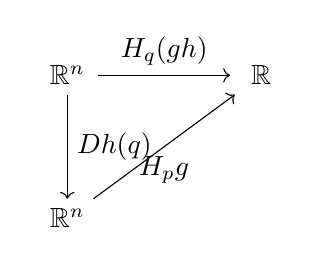
\begin{tikzpicture}
  \matrix (m) [matrix of math nodes, row sep=3.8em, column sep=4.8em, minimum width=2.2em]
  {
    \mathbb{R}^n & \mathbb{R} \\ 
     \mathbb{R}^n & \\ 
};
  \path[->]
  (m-1-1) edge node [above] {$H_q(gh) $} (m-1-2)
          edge node [auto] {$Dh(q) $} (m-2-1)
  (m-2-1) edge node [below] {$H_pg $} (m-1-2)
  ;
\end{tikzpicture}  

(quadratic) form $(H_pf)$ invariant under diffeomorphisms.


Let $C^2$ $f:M\to \mathbb{R}$.  \\
$\forall \,$ critical pt. $x$ of $f$, define \\
Hessian quadratic form
\[
\begin{aligned}
  & H_xf : M_x \to \mathbb{R} \\ 
  & H_xf : M_x \xrightarrow{ D\varphi_x } \mathbb{R}^n \xrightarrow{ H_{\varphi(x)}(f\varphi^{-1} ) } \mathbb{R}
\end{aligned}
\]
where $\varphi$ is any chart at $x$.

Thus, critical pt. of a $C^2$ real-valued function nondegenerate iff associated Hessian quadratic form is nondegenerate.  

Let $Q$ nondegenerate quadratic form on vector space $E$.

$Q$ negative definite on subspace $F \subset E$ if $Q(x)<0$ whenever $x\in F$ nonzero.

Index of $Q \equiv \text{Ind}Q$, is largest possible dim. of subspace on which $Q$ is negative definite.








cf. 1.1. Morse's Lemma of  Ch. 6, pp. 145, Morse Theory of Hirsch (1997) \cite{MHirsch1997}

\begin{lemma}[Morse's Lemma]
  Let $p\in M$ be nondegenerate critical pt. of index $k$ of $C^{r+2}$ map $f:M\to \mathbb{R}$, $1\leq r \leq \omega$.

  Then $\exists \, C^r$ chart $(\varphi,U)$ at $p$ s.t.
  \begin{equation}
    f\varphi^{-1}(u_1 \dots u_n) = f(p) - \sum_{i=1}^k u_i^2 + \sum_{i = k+1}^n u_i^2
  \end{equation}
  \end{lemma}

Let ${\,}^TQ \equiv Q^T$ denote tranpose of matrix $Q$.

\begin{lemma}
  Let $A = \text{diag}\lbrace a_1 , \dots , a_n \rbrace$ diagonal $n\times n$ matrix, with diagonal entries $\pm 1$.

  Then $\exists \, $ neighborhood $N$ of $A$ in vector space of symmetric $n\times n$ matrices, $C^{\infty}$ map
  \begin{equation}
P:N \to GL(n,\mathbb{R})
  \end{equation}
  s.t. $P(A)=I$, and if $P(B) = Q$, then $Q^T BQ = A$
\end{lemma}

\begin{proof}
  Let $B = [b_{ij}]$ be symmetri matrix near $A$ s.t. $b{11} \neq 0$ and $b_{11}$ has same sign as $a_1$.

    Consider $x=Ty$ where
    \[
\begin{aligned}
&  x_1 = \left[ y_1 - \frac{b_{12}}{b_{11}} y_2 - \dots - \frac{b_{1n}}{b_{11}} y_n \right] / \sqrt{ |b_n | } \\ 
& x_k = y_k \text{ for } k = 2, \dots n 
  \end{aligned}
    \]
  \end{proof}


\section{Lagrange multipliers}

From \emph{wikipedia:Lagrange multiplier}, \url{https://en.wikipedia.org/wiki/Lagrange_multiplier},
find local minima (maxima), pt. $a\in N$, s.t. $\exists \, $ neighborhood $U$ s.t. $f(x) \geq f(a)$ ($f(x) \leq f(a)$) \, $\forall \, x\in U$.

For $f:U\to \mathbb{R}$, open $U\subset \mathbb{R}^n$, find $x\in U$ s.t. $D_xf \equiv Df(x) =0$, check if Hessian $H_x f<0$.

Maxima may not exit since $U$ open.


References:

\href{http://www.math.uni.wroc.pl/~karch/analiza_nieliniowa/18_mnozniki-lagrangea.pdf}{Relative Extrema and Lagrange Multipliers}

Other interesting links:

\href{http://oai.cwi.nl/oai/asset/2552/2552A.pdf}{The Lagrange Multiplier Rule on Manifolds and Optimal Control of nonlinear systems}

\part{Classical Mechanics}

\problemhead{1.4 The altitude angle of the Sun, Japan Physics Olympiad (2014)} cf. Japan Physics Olympiad, (2014) \cite{Japa2014}.


\solutionhead{1.4 The altitude angle of the Sun, Japan Physics Olympiad (2014)}

\quad \\ 

$NC \equiv$ Niigata City, \\
$AM \equiv $ Amagi-san in Izu. \\

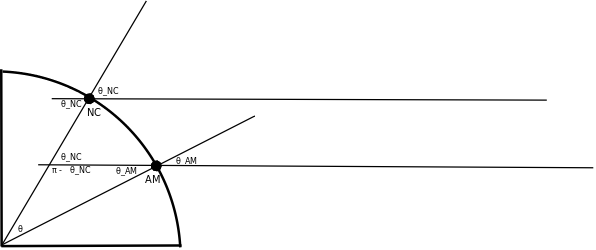
\includegraphics[scale=0.7]{./Prob1_4_altitude_angle_of_sun.png}

From all 3 internal angles of a triangle sum up to 180 degrees, or i.e. $\pi$ radians,
\[
\begin{gathered}
	\pi = \pi - \theta_{NC} + \theta_{AM} + \theta \Longrightarrow \boxed{ \theta = \theta_{NC} - \theta_{AM}} 
\end{gathered}
\]
So we've shown indeed that $\theta$ is the \textbf{difference between altitude angles of the Sun} at NC and AM, respectively.


From 
\[
\begin{gathered}
\begin{aligned}
	& C = 2 \pi R \\
 	& l_M = \theta R 
\end{aligned} \\
\frac{ l_M }{l} = \frac{ \theta R}{  \frac{\pi}{2} R } \text{or } \frac{ l_M}{l} = \frac{ 2 \theta}{ \pi} \\
 \Longrightarrow \theta = \frac{\pi}{2} \frac{ l_M}{l} = \frac{\pi}{2} \cdot \frac{334 \times 10^3 \, m}{ 10^7 m} \cdot \frac{ 180^{\circ} }{ \pi} = 3^{\circ}
\end{gathered}
\]

Advice, remember to draw a \emph{cross-section} to make diagram clear, rather than worry about "the other transverse dimension". Also, draw the lines literally parallel to the Sun because of how far away the Sun is and how large the Sun is.


\section{Structure of Galilean Space-Time}

cf. Sec. 3.1 - \emph{Structure of Galilean Space-Time} of Pr\'{a}staro (1996) \cite{Pras1996}.

Mechanics assumes a particular simple formulation if formulated with respect to some spacetime manifold.

In Galilean spacetime, it's possible to naturally recognize absolute objects, and others that depend on frames.

cf. Def. 3.1 of Pr\'{a}staro (1996) \cite{Pras1996}
\begin{definition}[Galilean spacetime structure]
\begin{enumerate}
	\item Galilean spacetime structure $:= (\mathcal{G}, g)$ where \\
	$\mathcal{G}$ is (fiber bundle space-time)
	\begin{equation}
		\mathcal{G} \equiv \lbrace \tau : M \to T \rbrace
	\end{equation}
	where \\
	$M = $ 4-dim. affine manifold (\textbf{space-time}); corresponding structure is $(M, \mathbf{M}, \alpha)$, \\
\item	$T = $ 1-dim. affine space (\textbf{time}), corresponding affine structure is $(T, \mathbf{T}, \beta)$
\item $\tau = $ surjective affine mapping, of constant rank $1$, s.t. $\forall \, p \in M$ associates its time $\tau(p) \in T$
\end{enumerate}

Put $\mathbf{S} = \text{ker}(\underline{\tau}) \equiv \text{ker}(D\tau)\in M$, \\
	where $\underline{\tau} \equiv D\tau$, $D$ is symbol of derivative.\\	
	Define 
	\[
	\begin{aligned}
	& g: M \to vS_2^0(M) \equiv M \times S_2^0(\mathbf{S}) \\ 
	& g(p) = (p, \underline{g})  \equiv (p, Dg) , \forall \, p \in M
	\end{aligned}
	\]
	where $\underline{g} \equiv Dg$ is a Euclidean structure on $\mathbf{S}$.  $g$ is called vertical metric field.
\end{definition}

Thus, given $(M, \mathbf{M}, \alpha)$, $\forall \, (O, \lbrace \mathbf{e}_i)_{1 \leq i \leq d}$, $\lbrace \mathbf{e}_i \rbrace_{i=1\dots d}$, is basis of $\mathbf{M}$, 
\[
M \cong \mathbb{R}^4, \text{and } \exists \, \lbrace x^{\alpha} : M = \mathbb{R}^4 \to \mathbb{R} \rbrace_{\alpha = 1 \dots 4}
\]

cf. 1.1.3 Principle of Relativity, pp. 9, 1 Basic Principles of Classical Mechanics, Arnold, Kozlov, Neishtadt (2006) \cite{AKN2006}.

direct product $E^3 \times \mathbb{R}\lbrace t \rbrace$ (spacetime) has natural structure of affine space \\
Galilean group is by def. group of all affine transformations of $E^3 \times \mathbb{R}$ that preserve time intervals and are isometries of space $E^3 \, \forall \,$ fixed $t\in \mathbb{R}$.  \\

Thus if 
\begin{definition}[Galilean group]\label{Def:GalileanGroup}
\textbf{Galilean group} is group of all affine transformations of $E^3 \times \mathbb{R}$ that preserve time intervals and are isometries of space $E^3 \, \forall \, $ fixed $t\in \mathbb{R}$. \\

Thus, if Galilean transformation $g$, 
\begin{equation}
\begin{aligned}
& g: E^3 \times \mathbb{R}\lbrace t\rbrace \to E^3 \times \mathbb{R} \lbrace t \rbrace \\
& g:(s,t) \mapsto (s', t')
\end{aligned}
\end{equation}
\begin{enumerate}
	\item $t_{\alpha} - t_{\beta} = t'_{\alpha} - t'_{\beta}$ \\
	\item if $t_{\alpha} = t_{\beta}$, then $|s_{\alpha} - s_{\beta} | = |s'_{\alpha} - s_{\beta}' |$
\end{enumerate}

\end{definition}

Consider $(s_a,t_a), (s_b, t_b)$, $t_a - t_b$, $|s_a - s_b|$.
\[
\begin{gathered}
\begin{aligned}
	& g(s_a, t_a) = (s'_a, t'_a) \\ 
	& g(s_b,t_b) = (s'_b, t'_b)
\end{aligned} \\
\begin{aligned}
& t_a' - t'_b = \pi_tg(s_a, t_a) - \pi_tg(s_b, t_b) = t_a - t_b \\ 
& |s_a' - s'_b| = | \pi_s g(s_a,t_a) - \pi_sg(s_b,t_b) | = |s_a-s_b|
\end{aligned}
\end{gathered}
\]

Galilean group $g$ acts on $\mathbb{R}^3\lbrace \mathbb{r} \rbrace \times \mathbb{R} \lbrace t \rbrace$. \\

\subsection{3 examples of Galilean transformations}

uniform motion with constant velocity $\mathbf{v}$:
\begin{equation}
g_1(\mathbf{r}, t) = (\mathbf{r} + \mathbf{v} t, t)
\end{equation}

translation of origin in spacetime
\begin{equation}
g_2(\mathbf{r}, t) = (\mathbf{r} + \mathbf{x} , t + \alpha )
\end{equation}

rotation of coordinate axes
\begin{equation}
g_3(\mathbf{r}, t) = (G \mathbf{r}, t)
\end{equation}
where $G: \mathbb{R}^3 \to \mathbb{R}^3$ is orthonormal transformation.

\begin{proposition}[Galilean transformation decomposition]
	$\forall \, $ galilean transformation $g: \mathbb{R}^3 \times \mathbb{R} \to \mathbb{R}^3 \times \mathbb{R}$ can be uniquely represented as composition $g_1g_2 g_3$
\end{proposition}
cf. Prop. 1.1 of Arnold, Kozlov, Neishtadt (2006) \cite{AKN2006} 

\begin{proof}
Consider affine transformation of $E^4 = E^3 \times \mathbb{R}$ of general form
\[
\begin{aligned}
& \mathbf{x} = A\mathbf{x}' + \mathbf{v} t' + \mathbf{a} \\ 
& t = \langle \mathbf{l} , \mathbf{x}' \rangle + kt' + s 
\end{aligned}
\]
$A \in \text{Mat}_{\mathbb{R}}(3,3)$, $\mathbf{v}, \mathbf{a}, \mathbf{l} \in \mathbb{R}^3$, $k, s \in \mathbb{R}$. \\


By galilean transformation (Def. \ref{Def:GalileanGroup}), $t_2 - t_1 = t_2' - t_1'$, so 
\[
\begin{gathered}
t_2 - t_1 = \langle \mathbf{l} , \mathbf{x}'_2 \rangle + k t'_2 + s - \langle \mathbf{l}, \mathbf{x}'_1 \rangle - k t'_1 - s = \langle \mathbf{l}, \mathbf{x}'_2 - \mathbf{x}'_1 \rangle + k (t'_2 - t'_1) = t'_2 - t'_1
\end{gathered}\]
	
Since each of the 3 components of $\mathbf{x}_2 - \mathbf{x}_1$ are arbitrary, $\mathbf{l} = 0$, $k=1$ clearly. Or, let $t=2 = t_1$. Then clearly $\mathbf{l}=0$. \\

By galilean transformation (Def. \ref{Def:GalileanGroup}), $|\mathbf{x}_2 - \mathbf{x}_1 | = |\mathbf{x}'_2 - \mathbf{x}'_1 |$ \\

Let $t_2 = t_1$. \\
\[
\begin{gathered}
|\mathbf{x}_2 - \mathbf{x}_1 | = |A\mathbf{x}'_2 + \mathbf{v} t'_2 + \mathbf{a} - A \mathbf{x}'_1  - \mathbf{v}t'_1 - \mathbf{a}| = | A (\mathbf{x}'_2 - \mathbf{x}'_1 ) + \mathbf{v} (t'_2 - t'_1) | = | A(\mathbf{x}'_2 - \mathbf{x}'_1)| = | \mathbf{x}'_2 - \mathbf{x}'_1 |
\end{gathered}\]
Now let $\mathbf{y} = \mathbf{x}'_2 - \mathbf{x}'_1$.
\[
|A\mathbf{y} |^2 = y^T A^T A y = y^T y 
\]
only if $A^T A = 1$. So $A$ orthonormal.

Thus we've found the \emph{general form of Galilean transformations}:
\begin{equation}\label{Eq:GeneralFormOfGalileanTransformations}
\boxed{ \begin{aligned} & \mathbf{x} = A \mathbf{x}' + \mathbf{v} t' + \mathbf{a}, \quad \, A\in O(3), \mathbf{v},\mathbf{a} \in \mathbb{R}^3, s\in\mathbb{R} \\
& t= t'+s \end{aligned} }
\end{equation}

Since orthogonal matrices form a 3 parameter family, $\text{dim}A + \text{dim}\mathbf{v} + \text{dim}\mathbf{a} + \text{dim}s = 3+ 3+3 + 1 = 10$ independent parameters.

Recall that $g_1(\mathbf{r}, t) = (\mathbf{r} + \mathbf{v} t, t)$, $g_2 (\mathbf{r}, t) = (\mathbf{r} + \mathbf{a}, t+s)$, $g_3 (\mathbf{r}, t) = (A\mathbf{r}, t)$, then $g= g_1g_2g_3$.

\end{proof}

Introduce $E^3$ a "fixed" reference frame by fixing pt. $o \in E^3$ and choosing 3 mutually perpendicular axes.

\emph{inertial frame} - frame moving uniformly and rectilinearly with respect to fixed pt. $o \in E^3$; $\forall $ element of Galilean group transforms fixed frame into inertial frame. \\

action of galilean group on $E^3 \times \mathbb{R}$ can be extended to action on $E^3 \times \dots \times E^3 \times \mathbb{R}$ by the rule: \\
if $g: (s,t) \to (s',t')$, then \\
\phantom{if} $g(s_1, \dots s_n, t) = g(s_1' , \dots s_n', t')$ \\

Galileo-Newton principle of relativity asserts that Newton's equations invariant under Galilean transformation group in inertial reference frame.

$M = $ 4-dim. affine manifold (spacetime). Recall definition of an \emph{affine manifold} from \href{https://en.wikipedia.org/wiki/Affine_manifold}{wikipedia}.

Affine manifold $M$ is real manifold with charts $\psi_i : U_i \to \mathbb{R}^n$, s.t. $\psi_i \circ \psi_j^{-1} \in \text{Aff}(\mathbb{R}^n)$ \, $\forall \, i ,j$ where $\text{Aff}{(\mathbb{R}^n)}$ denotes Lie group of affine transformations; \\

Recall the definition of a \emph{Lie group of affine transformations}, $\text{Aff}{(\mathbb{R}^n)}$, the "affine structure", \footnote{\href{http://citeseerx.ist.psu.edu/viewdoc/download?doi=10.1.1.627.5443&rep=rep1&type=pdf}{"Affine structures on Lie algebras" by Michel Goze and Elisabeth Remm}},

\begin{definition}[Lie group of affine transformations, affine structure]
	\begin{equation}
	\text{Aff}(\mathbb{R}^n) = \lbrace \left(\begin{matrix} A & b \\ 0 & 1 \end{matrix} \right) | A \in GL(n, \mathbb{R}), b \in \mathbb{R}^n \rbrace
	\end{equation}
	s.t. $\left(\begin{matrix} A & b \\ 0 & 1 \end{matrix} \right)$ acts on real affine space $\widetilde{\mathbb{R}^n}$ by 
	\begin{equation}
	\left( \begin{matrix} A & b \\ 0 & 1 \end{matrix} \right) \left( \begin{matrix} v \\ 1 \end{matrix} \right) = \left( \begin{matrix} Av + b \\ 1 \end{matrix} \right) 
	\end{equation} where $A \in GL(n, \mathbb{R})$, $b\in \mathbb{R}^n$, where $(v,1)^T \in \widetilde{\mathbb{R}^n}$
\end{definition}

If changing notation, and keeping in mind that $n=4$, $\psi_j \equiv y(v_{(y)}) \to \mathbb{R}^n$, \\
$ \begin{aligned} & \quad \\ 
\psi_i \equiv & x : U_{(x)} \to \mathbb{R}^n \\ 
& x(p) \in \mathbb{R}^n, x_i(p) \in \mathbb{R} \end{aligned}$ \\

Rewrite the Eq. \ref{Eq:GeneralFormOfGalileanTransformations} in matrix form:
\[
\begin{gathered}
\begin{aligned}
& \mathbf{x} = A \mathbf{x}' + \mathbf{v} t + \mathbf{b} \\ 
& t = t'+ s, \, A \in O(3), \, \mathbf{v}, \mathbf{b} \in \mathbb{R}^3, \, s \in \mathbb{R}
\end{aligned} \\
\left( \begin{matrix} A & \mathbf{v} & \mathbf{b} \\ 0 & 1 & s \\ 0 & 0 & 1 \end{matrix} \right) \left(\begin{matrix} \mathbf{x}' \\ t' \\ 1 \end{matrix} \right) = \left( \begin{matrix} \mathbf{x} \\ t  \\ 1 \end{matrix} \right) \text{ or } \left( \begin{matrix} A & \mathbf{v} \\  0 & 1 \end{matrix} \right) \left( \begin{matrix}\mathbf{x}' \\ t' \end{matrix} \right) + \left( \begin{matrix} \mathbf{b} \\ s \end{matrix} \right) = \left(\begin{matrix} \mathbf{x} \\ t \end{matrix} \right)
\end{gathered}
\]

Consider $y$ being standard Euclidean coordinates in fixed frame $o$. $x$ then is coordinates in any other inertial frame.

$T =$ 1-dim. affine space since affine structure $(T, \mathbf{T}, \beta)$ is s.t. $T\in \mathbb{R}$, $\mathbf{T} \in \mathbb{R}$, $\begin{aligned} & \quad \\ 
& \beta : \mathbf{T} \times T \to T \\
& \beta(s,t') = t' + s = t\end{aligned}$ \\

Holm (2011) \cite{Holm2011}

\section{Kinematics}

\subsection{Kinematics Problems from Irodov}

cf. Irodov (1981) \cite{Irod1981}

\solutionhead{1.1} If we assume that the raft goes along downstream with no further "rowing", \\
$l \equiv $ distance raft travels for total time $T$ = 6.0 \, km \\
$v_d \equiv $ downstream speed $=$ raft speed \\
$\tau = 60 \, \text{mins} = $ time before motorboat turning back \\
$v_m \equiv $ motorboat speed \\

\[
\begin{gathered}
	\frac{l}{v_d} = \tau + \frac{ \tau (v_m + v_d) - l }{ v_m - v_d} = \frac{ \tau (2 v_m) - l }{ v_m - v_d } \text{ or } 
\end{gathered} \quad \quad \, \begin{gathered}
(v_m - v_d) l = 2 \tau v_m v_d - l v_d \\
v_m l = 2\tau v_m v_d \\
\boxed{ v_d =  \frac{l}{2\tau } }= \frac{6.0 \, km }{ 2 \cdot 60 \, \text{mins}} = 0.05 \,  \text{km / min}
\end{gathered}
\]

\solutionhead{1.2} The speed formula, recall, is $L = \overline{v} T$, or $\overline{v} = \frac{L}{T}$. 
\[
v_0 t_0 = \frac{L}{2} \text{ or } t_0 = \frac{L}{2 v_0} 
\]
\[
\begin{gathered}
	l_1 = v_1 \frac{T_1}{2} \\
	l_2 = v_2 \frac{T_1}{2} 
\end{gathered} \text{ and }
l_1 + l_2  = \frac{L}{2} \text{, so } L = v_1 T_1 + v_2  T_1 
\]
\[
\Longrightarrow \overline{v} = \frac{L }{ \frac{L}{2v_0} + \frac{L}{v_1 + v_2} } = \frac{2 v_0 (v_1 + v_2) }{ 2v_0 + v_1 + v_2}
\]

\solutionhead{1.3} Given \\
$w = 5.0 \, m/s^2 = $ constant acceleration and deceleration \\
$\tau = 25 \, \text{sec.} = $ total time of motion \\
$\overline{v} = 72 $ km / hr. $=$ average velocity during that time ($\tau$?) \\

Recall that
\[
\begin{gathered}
	a = a(t) = \frac{dv}{dt} \text{ so if $a$ constant, then} v(t) - v_0 = at \text{ and since } v(t) = frac{dx}{dt} \text{ so } \\
 	x(t) = x_0 + v_0t + \frac{1}{2} at^2 \\
 	d = x(t) - x_0 = t(v_0 + \frac{a}{2} t) = \frac{v- v_0}{a} (v_0 + \frac{v-v_0}{2}) = \frac{v^2 - v_0^2 }{2a } \text{ or } v^2 - v_0^2  =2ad
\end{gathered}
\]
Then 
\[
\frac{v^2}{2w} + \frac{v^2}{2w} + vT_2 = L \text{ or } \frac{v^2}{w} + vT_2 = L
\]
Also
\[
\tau = \frac{v}{w} + T_2 + \frac{-v}{-w} = \frac{2v}{w} + T_2 \text{ or } (\tau - T_2) \left( \frac{w}{2} \right) = v
\]
Then
\[
\begin{gathered}
	\overline{v} = \frac{ \frac{v^2}{w} + vT_2}{ \tau} \text{ or } \overline{v}\tau = \frac{v^2}{w} + wT_2 \\
	\Longrightarrow \overline{v}\tau = v \left( \frac{v}{w} + T_2 \right) = v ( \frac{\tau - T_2}{2} + T_2 ) = \frac{w}{2} ( \tau - T_2) ( \frac{\tau + T_2}{2} ) \\
	4\overline{v} \tau = w (\tau^2 - T_2^2) \text{ or } wT_2^2 = w T^2 - 4 \overline{v} \tau \\
	\Longrightarrow \boxed{ T_2  = \sqrt{ \tau^2 - \frac{4\overline{v} \tau}{w} } }
\end{gathered}
\]

\solutionhead{1.5; particles collide} 

\textbf{Hint}: \emph{change reference frames}, in particular, into frame of references of particles 1 or 2, respectively. \\
Consider, by label symmetry, reference frame of particle 1:
\[
\begin{gathered}
	\begin{aligned}
		& r'_1 = r_1- r_1 = 0 \\
		& r'_2 = r_2 - r_1 
	\end{aligned} \quad \quad \, 
	\begin{aligned}
		& v_1' = v_1 - v_1 = 0 \\
		& v'_2 = v_2 - v_1
	\end{aligned}
\end{gathered}
\]
On order for a collision, in reference frame of particle 1, particle 2 will need to approach or travel towards the origin from $r'_2=  r_2 - r_1$; consider  \\
$v_2' \parallel = -r'_2$ i.e. $v_2 - v_1 \parallel -(r_2 - r_1)$, otherwise particle 2 would never reach origin where particle 1 is
\[
\Longrightarrow \boxed{ \frac{ \textbf{v}_2-  \mathbf{v}_1}{ \| \mathbf{v}_2 - \mathbf{v}_1 \| } = \frac{ -(\mathbf{r}_2 - \mathbf{r}_1) }{ \| \mathbf{r}_2 - \mathbf{r}_1 \| } }
\]

\solutionhead{1.6} $v_0 = 30 \, km/hr = $ ship moves along equator to the east with speed $v_0$ \\
$\varphi = 60^{\circ} = $ southeastern wind blows at angle $\varphi$ to equator \\
$v_w = 15 \, km /h = $ wind speed \\
$v_w = v_{w,x} \mathbf{e}_x + v_{w,y} \mathbf{e}_y$ \\
If southeastern wind means \emph{it comes \textbf{from} the south east}, then we have
\[
\begin{gathered}
	v_w' = v_w - v_0 = (-v_w \cos{\varphi} - v_0) \mathbf{e}_x + v_w s{\varphi} \mathbf{e}_y \\
	\| v_w' \|^2 = v_w^2 c^2{\varphi} + 2v_w v_0 c{\varphi} + v_0^2 + v_w^2 s^2{\varphi} = v_w^2 + v_0^2 + 2v_w v_0 c{\varphi} = v_w^2 + v_0^2 + 2v_w v_0 \frac{1}{2} \approx 39.7 \, km /h \approx 40 \, km/h \\
	\varphi' = \arctan{ \left( \frac{ -v_w s{\varphi} }{ v_w c{\varphi} + v_0}  \right) } = \arctan{ \left( \frac{-v_w \sqrt{3} / 2}{ v_w /2 + v_0 } \right) } \approx -19.1^{\circ}
\end{gathered}
\]

cf. \url{https://physics.stackexchange.com/questions/126268/relative-wind-velocity-explanation} for southeastern wind explanation.

\solutionhead{1.7}

2 swimmers leave pt. A, pt. A lie right across point B. \\
stream velocity $v_0 = 2.0 \, \text{km}/\text{hr}$ \\
velocity $v'$ of each swimmer with respect to water $=2.5$ km/hr \\
Now $(\mathbf{v}_A + \mathbf{v}_0) T_A = \mathbf{x}_A$ and so in components, $v_{A,x} T_A = L$ and $(v')^2 = (v_{A,x})^2 + v_0^2$ or $v_{A,x} = \sqrt{(v')^2 - v_0^2}$ \\

$T_{B,1} = $ time to swim across the river \\
$T_{B,2} = $ time to walk the distance he has been carried. \\

Since $(\mathbf{v}_B + \mathbf{v}_0) T_{B,1} = \mathbf{x}_{B,1}$ with $\begin{aligned} & \quad \\ 
	& v' T_{B,1} = L \\
	& v_0 T_{B,1} = y_B \end{aligned}$ \\

$T_A = T_{B,1} + T_{B,2}$ since both swimmers reach the destination simultaneously. 

\[
\Longrightarrow \frac{ L}{v_{A,x}} = \frac{L}{v'} + \frac{v_0 L}{uv'} \text{ or } u = \frac{v_0 / v'}{ \frac{1}{ v_{A,x}} - \frac{1}{v'} } = \boxed{ \frac{ v_0}{ \frac{v'}{ \sqrt{ (v')^2 - v_0^2} } - 1 }  }= 3.0 \, km/hr
\]

\solutionhead{1.8}

Buoy anchored at the middle of a river. \\
$v_s = $ stream velocity \\

\[
\begin{gathered}
(v_A + v_s) T_{A,1} = L = (v_A -v_s) T_{A,2} \\
\Longrightarrow (\eta + 1) v_s T_{A,1} = L = (\eta - 1) v_s T_{A,2}	
\end{gathered}
\]
where $T_{A,1} = \frac{L}{ (\eta + 1) v_s}$ is the time going away from the buoy to a distance L for person A, and $T_{A,2} = \frac{L}{ (\eta - 1) v_s} $ is the time to go back.

B moves away along the mutually perpendicular straight lines across the river. Then
\[
\begin{gathered}
	(\mathbf{v}_B + \mathbf{v}_s) T_{B,1} = \mathbf{x}_B \\
	v_{B,x} T_{B,1} = L \\
	v_B^2  = (\eta v_s)^2 = v_{B,x}^2 + v_{B,y}^2 = v_{B,x}^2 + v_s^2
\end{gathered}
\]
Now $T_{B,1} = T_{B,2}$, i.e. the time to go away from the buoy is equal to the time to go back to the buoy, and so
\[
2 T_{B,1} = \frac{2L}{ \sqrt{ (\eta v_s)^2 - v_s^2} } = \frac{2L}{ v_s \sqrt{ \eta^2 - 1} }
\]
Thus,
\[
\begin{gathered}
	\frac{\tau_A}{ \tau_B} = \frac{T_{A,1} + T_{A,2} }{ T_{B,1} + T_{B,2}} = \frac{ \frac{2\eta}{\eta^2 - 1} }{ \frac{2 }{\sqrt{\eta^2 - 1} } } = \boxed{ \frac{ \eta}{ \sqrt{ \eta^2 - 1 } } } \approx 1.81 \approx 1.8
\end{gathered}
\]

\solutionhead{1.10}

For body 1 going straight up, $y_1 = v_0 t - \frac{1}{2} gt^2$ and there's no horizontal, $x_1$, translation. \\

For body 2, the coordinates over time are the following:
\[
\begin{aligned}
	& y_2 = v_0s{\theta} t - \frac{1}{2} gt^2 \\
	& x_2 = v_0 c{\theta} t
\end{aligned}
\]

\[
\begin{gathered}
	\| \mathbf{x}_2 - \mathbf{x}_1 \|^2 = (v_0 t(1 - s{\theta}))^2 + (v_0 c{\theta}t)^2 = (v_0 t)^2 [ 2 - 2 s{\theta}] = 2(v_0t)^2 (1- s{\theta}) \\
	\| \mathbf{x}_2 - \mathbf{x}_1 \| = \boxed{ v_0 t \sqrt{2} \sqrt{1 - s{\theta}} } = 25 (1.7) \sqrt{2} \sqrt{ 1 - \sqrt{3} / 2 } \approx 22
\end{gathered}
\]

\solutionhead{1.11} 2 particles move in a uniform gravitational field with acceleration $g$.  \\
At initial moment, the particles were located at 1 pt. and moved with velocities $v_1 = 3.0 \, m/s$, $v_2 = 4.0 \, m/s$ horizontally in opposite directions. \\
Typically, gravitational field is \textbf{vertical}:
\[
\begin{gathered}
\begin{aligned} 
	& v_{1y} = -gt \\
	& v_{1x} = -v_1 
\end{aligned} \quad \quad \, \begin{aligned}
& v_{2y} = -gt \\
& v_{2x} = v_2 
\end{aligned} \\
	\begin{aligned}
		& y_1 = -\frac{1}{2} gt^2 \\
		& x_1=  -v_1 t
	\end{aligned} \quad \quad \, \begin{aligned}
	& y_2 = \frac{-1}{2} gt^2 \\
	& x_2 = v_2 t
\end{aligned}
\end{gathered}
\]

mutually perpendicular: $\mathbf{v}_1 \cdot \mathbf{v}_2 = 0 = -v_1 v_2 + g^2 t^2$ or $t = \frac{ \sqrt{v_1 v_2}}{g}$ \\

\[
\begin{gathered}
	\| \mathbf{x}_2 - \mathbf{x}_1 \|^2 = ((v_2 + v_1)t)^2 + 0 = (v_2 + v_1)^2 \frac{v_1 v_2}{g^2} \text{ or } \\
	\boxed{ \| \mathbf{x}_2 - \mathbf{x}_1 \| = \frac{ (v_1 + v_2) }{g} \sqrt{v_1 v_2} } = \frac{ 7 }{ 9.8 \, m/s^2} 2 \sqrt{3} = 2.5 \, m
\end{gathered}
\]

\problemhead{1.12} Three points are located at the vertices of an equilateral triangle whose side equals $a$. They all start moving simultaneously with velocity $v$ constant in modulus, with the first point heading continually for the second, the second for the third, and the third for the first. How soon will the points converge?

\solutionhead{1.12} By symmetry at any time (point), consider component of $\mathbf{v}$ towards triangle center (EY: this is the key insight; breakup components of $\mathbf{v}$ to be along "radial" distance traveled, not just along Cartesian x and y).

By symmetry of the problem, $v$ will always be along an equilateral triangle side, for each moving point.

Let $\theta_0 = 30^{\circ}$.

Then
\[
\cos{\theta_0} = \frac{v_r}{v} \text{ or } v\cos{\theta_0} = v_r
\]
\[
\cos{\theta_0} = \frac{a/2 }{ d} \text{ or } d = \frac{a/2}{ \cos{\theta_0}} = \frac{a/2}{ \sqrt{3}/2 } = \frac{a}{\sqrt{3}}
\]
where $d$ is the distance from a point to the center of the triangle.

\[
v_x = \frac{ds}{dt} \Longrightarrow T = \int dt = \int \frac{ds}{v_x} = \int^0_{a/\sqrt{3}} \frac{ds}{ -v\cos{\theta_0}} = \frac{-a}{\sqrt{3}} \frac{1}{v\sqrt{3}/2} = \frac{2a}{3v}
\]


\problemhead{1.13} Point $A$ moves uniformly with velocity $v$ so that the vector $\mathbf{v}$ is continually "aimed" at point $B$ which in its turn moves rectilinearly and uniformly with velocity $u < v$. At the initial moment of time $\mathbf{v} \perp \mathbf{u}$ and the points are separated by a distance $l$. How soon will the points converge?

\solutionhead{1.13} Choose $\mathbf{u}$ to be in the $x+$ direction: $\mathbf{u} = u\mathbf{e}_x$. 

Condition: Point A reaches point B, so total x-distance traveled during time interval $T$ is the same:
\begin{equation}
	\int_0^T v \cos{\alpha} dt = u T
\end{equation}

Now consider the "straight line distance" between point A and point B. We're given at the initial moment of time $\mathbf{v} \perp \mathbf{u}$, that the points are separated by distance $l$.

Now think in terms of displacement in very short time interval $\Delta t$. Point A is traveling distance $v\Delta t$ towards point B in a straightline. But point B is moving away with component along the straight line by distance $u\cos{\alpha} \Delta t$.

The total straight line distance point A has to cover is distance $l$. The net distance traveled in $\Delta t$, $v\Delta t - u\cos{\alpha} \Delta t$ must sum up to $l$ in order for point A and point B to converge. For a small time interval $\Delta t$, the $-u\cos{\alpha}$ term already is accounting for how much point B is moving away and $v$ term accounts for how fast point A is traveling the distance towards point B.

So
\begin{equation}
	\int_0^T (v-u\cos{\alpha}) dt = l = vT - u \left( \frac{u T}{v} \right) \text{ or } \boxed{ T = \frac{lv}{ v^2 - u^2 } }
\end{equation}

\url{https://physics.stackexchange.com/questions/568531/why-is-the-following-equation-not-correct}
\url{https://www.physicsforums.com/threads/a-question-of-kinematics-involving-a-changing-velocity-vector.975126/post-6210692}

\section{Fundamental Theorems of (Classical) Dynamics}

cf. Sec. 3.4 - \emph{Fundamental Theorems of Dynamics} of Pr\'{a}staro (1996) \cite{Pras1996}.

cf. Thm. 3.20 of Pr\'{a}staro (1996) \cite{Pras1996}
\begin{theorem}[Momentum Theorem]
	Variation of the free part of momentum of the observed motion of 1 body, in time interval $\Delta t \equiv [0, t]$ is equal to the corresponding impulse:
	\begin{equation}
	I[0,t] \equiv \int_0^t Fdt \equiv \left( \int_0^t F^j dt \right) \mathbf{e}_j
	\end{equation}
	where $\lbrace \mathbf{e}_j \rbrace_{1 \leq j \leq 3}$ is a fixed basis of $\mathbf{S}$
	\begin{equation}
		\overline{p}_{\psi}(t) - \overline{p}_{\psi}(0) = I[0,t]
	\end{equation}
\end{theorem}

\begin{proof}
	\[
\begin{gathered}
\overline{p}_{\psi} = \mu \ddot{m}_{\psi} = \overline{f}_{\psi} \Longrightarrow \dot{ \overline{p}_{\psi}} = \dot{p}^j \mathbf{e}_j = F^j \textbf{e}_j \Longrightarrow \int_{[0,t]} \dot{p}^j dt = \int_{[0,t]}F^j dt
\end{gathered}
	\]
	\end{proof}

\subsection{Coordinate transformation}

For $(U, \varphi)$, $(V, \psi)$ charts on $M$, s.t. $\begin{aligned} & \quad \\ 
	& \varphi : U \to \mathbb{R}^n \\
	 & \psi: V \to \mathbb{R}^n \end{aligned}$, \quad \, $\begin{aligned} & \quad \\ 
	 & \varphi^i \equiv x^i \\
	 & \psi^j \equiv y^j \end{aligned}$, then consider 
\[
\begin{gathered}
\psi(p) = y = \psi \circ \varphi^{-1} \circ \varphi(p) = \psi \circ \varphi^{-1}(x) = y(x)
\end{gathered}  
\]

Consider $f: M \to M$ that is a coordinate transformation (bijective). Under this coordinate transformation, transformation of the components of the same vector $X = Y$ is the push-forward:

\begin{equation}
	Y^j = X^i \frac{\partial y^j}{\partial x^i}
\end{equation}

Correspondingly, basis transformation described by 
\begin{equation}
	\frac{\partial }{ \partial x^j }= \frac{\partial y^k }{ \partial x^j} \frac{ \partial }{ \partial y^k}  \text{ or  } \frac{\partial }{\partial y^k} = \left[  \left( \frac{\partial y}{ \partial x} \right)^{-1} \right]_k^{\, \, j} \frac{ \partial }{ \partial x^j } = \left( \frac{ \partial x^j}{ \partial y^k} \right) \frac{ \partial }{ \partial x^j}
\end{equation} 

Then we can show that indeed $Y = X$ under coordinate transformations:
\begin{equation}
	Y = X = Y^k \frac{\partial }{\partial y^k} = X^j \frac{ \partial }{ \partial x^j}
\end{equation}

Also, for $a_i = b_j \frac{ \partial y^j}{\partial x^i}$, the pull back describing how 1-form components transform, consider the inner product:
\begin{equation}
\begin{gathered}
	b(Y) = b_i dy^i \left( Y^k \frac{\partial }{ \partial y^k} \right) = b_i Y^i = b_i X^k \frac{\partial y^i}{\partial x^k} = b_i \frac{\partial y^i }{\partial x^k} X^k = a_k X^k = a(X)
\end{gathered}
\end{equation}

$\Longrightarrow$ inner product preserved under coordinate transformation, i.e. invariance of inner product.





\subsection{Transformation of reference frames}

cf. Sec. 4.2.1 "Transformation of reference frames", Kambe (2009) \cite{TKambe2009}.

Let us take pt. $\mathbf{y}_b$ fixed to body, \\
located at $\mathbf{x} = X^1 \mathbf{e}_1 + X^2 \mathbf{e}_2 + X^3 \mathbf{e}_3 = X^i \mathbf{e}_i$ at $t=0$, \\
where $\mathbf{e}_i$ ($i=1,2,3$) are orthonormal basis fixed to space $F \equiv$ nonrotating \textbf{fixed} space (inertial space) \\

By transformation matrix $A = (A^i_{ \, \, j }) \in \text{SO}(3)$, initial pt. $\mathbf{x} = (X^i)$ mapped to current pt. $\mathbf{y}_b$ at time $t$.
\begin{equation}
\mathbf{y}_b(t) = A(t) \mathbf{x} = y^i (t) \mathbf{e}_i, \quad \, y^i(t) = A^i_{ \, \, j}(t)X^j
\end{equation}
cf. Eq. (4.14) of Kambe (2009) \cite{TKambe2009}.

i.e.

\[
\begin{gathered}
\mathbf{y}_b(t) = A(t) \mathbf{x} = A^i_{\,\, k} e_i \otimes e^k x^l e_l = A^i_{ \, \, k} X^k e_i = y^i(t) e_i
\end{gathered}
\]

EY: Observe that $A(t)$, $t\in [0,t]$ is a curve in $\text{SO}(3)$.

In other words, we considered a point in the fixed frame $F$ given by frame $\lbrace \mathbf{e}_i \rbrace$:
\[
\mathbf{x} = X^i \mathbf{e}_i \text{ at } t = 0
\]

Then, we considered an "active" rotation $A \in SO(3)$ of this point, so 
\begin{equation}
	\mathbf{y}(t) = A(t) \mathbf{x} = A^i_{ \, \, j}(t) X^j \mathbf{e}_i = y^i(t) \mathbf{e}_i
\end{equation}
Indeed, consider $A = \left[ \begin{matrix} c & -s & \\ s & c & \\ & & 1 \end{matrix} \right]$. Then $A$ would rotate points in the $x-y$ plane, such as $[1, 0, 0]$, $[0, 1, 0]$ counter-clockwise in the positive $z$ axis direction.

On the other hand, relative to body frame $F_B$, which is the frame instantaneously fixed to the moving body. \\
For the same pt., $\mathbf{y}_b(t)$, fixed to body, is
\[
\mathbf{Y}(=\mathbf{y}_b) = Y^1 \mathbf{b}_1 + Y^2 \mathbf{b}_2 + Y^3 \mathbf{b}_3 = Y^i \mathbf{b}_i
\]
where $\mathbf{b}_i$ ($i=1,2,3$) are orthonormal basis fixed to body which coincided with $\mathbf{e}_i$ ($i=1,2,3$) at $t=0$. 

From property of a rigid body, it's required that $Y^i = X^i$ which don't change with $t$.

According to Sec. 1.5.1(b) (Kambe (2009) \cite{TKambe2009}), basis transformation written as (1.40) Kambe(2009) \cite{TKambe2009}, where 

\begin{equation}
\begin{gathered}
	\mathbf{b}_i = \mathbf{b}_i(t) = \mathbf{e}_j B^j_{\, \, i}(t) \\
		\text{ Then } \mathbf{Y} = Y^i \mathbf{b}_i = Y^i \mathbf{e}_j B^j_{ \, \, i} = \mathbf{e}_j B^j_{\, \, i } Y^i
\end{gathered}
%\mathbf{b}_k(t) = B_k^{ \, \, j}(t) \mathbf{e}_j \text{ hence } Y= Y^k \mathbf{b}_k = Y^k B_k^{ \, \, j} \mathbf{e}_j
\end{equation} 
(4.10) Kambe (2009) \cite{TKambe2009}, where $B = (B_k^{\, \, j}) \in \text{SO}(3)$, i.e. $BB^T = 1$. \\

Note that 
\begin{equation}
	\mathbf{Y} = Y^i \mathbf{b}_i = \mathbf{e}_j B^j_{\, \, i} Y^i = A^j_{\, \, k} X^k \mathbf{e}_j 
\end{equation}
implies that $B: F' \to F$ where $F'$ rotating frame, $F$ fixed frame, i.e. $B$ is a coordinate transformation from coordinates in the $F'$ rotating frame into coordinates in the $F$ fixed frame.

Indeed, consider 
\[
B = \left[ \begin{matrix} c & -s & \\ s & c & \\ & & 1 \end{matrix} \right]. \text{ Then } B \left[ \begin{matrix} 1 \\ 0 \\ 0 \end{matrix} \right] = [c, s, 0] (\text{in $\lbrace \mathbf{e}_j \rbrace$ frame})
\]

%Now $A = B$ because consider a basis element as the starting vector. So if $\mathbf{x} = \delta_i^{ \, \, k} \mathbf{e}_k$, then
%\[
%\begin{gathered}
%	\mathbf{y}_b(t) = A(t) \mathbf{x} = A^i_{ \, \, k} e_i \otimes e^k \delta_l^{\, \, j} \mathbf{e}_j = A^i_{ \, \, j} e_i \delta_l^{ \, \, j} = A^i_{\, \, l} \mathbf{e}_i
%\end{gathered}
%\]
%Now
%\[
%\begin{gathered}
%Y^i \mathbf{b}_i = \delta^i_{\, \, l} B^k_{ \, \, i}(t) \mathbf{e}_k = B^k_{ \, \, l}(t) \mathbf{e}_k
%\end{gathered}
%\]
%where $Y^i = \delta ^i_{\, \, l}$ because in the beginning, $\mathbf{Y}$ coincided with a basis vector $\mathbf{e}_l$.

%Thus, since $Y^i \mathbf{b}_i = \mathbf{Y} = \mathbf{y}_b(t)$, then $\boxed{A = B}$.

%Now for 
%\[
%\begin{gathered}
%A(t) : \mathbf{x} \mapsto \mathbf{y}_b(t) \\
%y^i_b = A^i_{ \, \ ,j} x^j
%\end{gathered}
%\]

%Now 
%\[
%\begin{gathered}
%\mathbf{b}_k(t) = B^i_{\, \, k}(t) \mathbf{e}_i \\
%\mathbf{Y} = Y^k\mathbf{b}_k = Y^k B^i_{ \, \, k}(t) \mathbf{e}_i 
%\end{gathered}
%\]

%Since $\mathbf{Y} = \mathbf{y}_b(t)$, then 
%\[
%Y^k B^i_{\,\, k}(t) = A^i_{\,\, j}x^j 
%\]
%So $X = Y$.

Now recall that $\mathbf{x} = X^i \mathbf{e}_i$ at $t=0$. $\mathbf{Y} = Y^i \mathbf{b}_i$ and $\lbrace \mathbf{b}_i \rbrace$ frame axes had coincided with $\lbrace \mathbf{e}_i \rbrace$ frame axes at $t=0$. $Y^i$'s are constant, so $Y^i = X^i$

So for 
\begin{equation}\label{Eq:ActiveAndPassiveRotationsEqual}
\begin{gathered}
\mathbf{Y} = Y^i \mathbf{b}_i = \mathbf{e}_j B^j_{\, \, i} Y^i = A^j_{\, \, k}(t) X^k \mathbf{e}_j \Longrightarrow B^j_{\, \, i} Y^i = A^j_{\, \, k}(t) X^k = A^j_{\, \, i} Y^i \text{ so } \boxed{ B = A } \text{ since $X^i$ arbitrary }
\end{gathered}
\end{equation}

For the basis transformation derivation, recall the push forward transformation (cf. Kambe (2009) \cite{TKambe2009}),

\[
\begin{gathered}
	\begin{aligned}
	& \phi : M \to N \\
	& \phi_* : T_xM \to T_y N \\
	& y = \phi(x) = F(x)
	\end{aligned} \\
\begin{aligned} 
& Y = \phi_* X = F_* X = \left. \frac{d}{dt} (F(p(t))) \right|_{t=0} \\
& Y^k = (\phi_* X)^k = \left( \frac{ \partial F^k }{ \partial x^j } \right) X^j \\
& Y = \phi_* X = \phi_* \left[ X^j \frac{ \partial }{ \partial x^j } \right] = X^j \phi_* \left[ \frac{ \partial }{ \partial x^j } \right] = X^j \frac{ \partial y^k}{ \partial x^j} \frac{ \partial }{ \partial y^k } = Y^k \frac{ \partial }{ \partial y^k } \\
& Y^k  = \frac{ \partial y^k }{ \partial x^j } X^j
\end{aligned} 
\end{gathered}
\]

\subsubsection{Direction Cosine Matrix (DCM)}

cf. pp. 134, 4.1 "The Independent Coordinates of a Rigid Body", Goldstein, Poole, Safko (2001) \cite{GPS2001}

Consider frame $F, \, \lbrace \mathbf{e}_1, \mathbf{e}_2, \mathbf{e}_3 \rbrace$, \\
\phantom{Consider} frame $F', \lbrace \mathbf{e}'_1, \mathbf{e}'_2, \mathbf{e}'_3 \rbrace$ 

If 
\[
\begin{gathered}
	\mathbf{e}_i' = C_{ij} \mathbf{e}_j
\end{gathered}
\]
and so then
\[
\begin{gathered}
	\mathbf{e}'_i \cdot \mathbf{e}_k = C_{ij} \delta_{jk} = C_{ik} \\
	\Longrightarrow \mathbf{e}_i' = (\mathbf{e}_i' \cdot \mathbf{e}_j ) \mathbf{e}_j
\end{gathered}
\]
So for $\mathbf{r}' = y^i \mathbf{e}_i' = x^j \mathbf{e}_j$, 
\begin{equation}\label{Eq:DirectionCosineMatrixCoordinateTransformation}
\begin{gathered}
	\Longrightarrow y^k = x^j (\mathbf{e}_k' \cdot \mathbf{e}_j )  \text{ or } y^i = (\mathbf{e}'_i \cdot \mathbf{e}_j) x^j
\end{gathered}
\end{equation}

So $\cos{\theta_{ij}} = \mathbf{e}_i' \cdot \mathbf{e}_j$ completely specifies the orientation of $F'$ relative to $F$.

Now use this fact, that $\mathbf{e}_m \cdot \mathbf{e}_m' = \delta_{mm'}$, to show that
\[
\begin{gathered}
	\mathbf{e}_m \cdot \mathbf{e}_m' = \delta_{mm'} = (\mathbf{e}_m \cdot \mathbf{e}'_l ) \mathbf{e}'_l \cdot (\mathbf{e}_{m'} \cdot \mathbf{e}'_{l'}) \mathbf{e}'_{l'} = (\mathbf{e}_m \cdot \mathbf{e}'_l)(\mathbf{e}_{m'} \cdot \mathbf{e}'_{l'}) \delta_{ll'} = (\mathbf{e}'_l \cdot \mathbf{e}_m )( \mathbf{e}'_l \cdot \mathbf{e}_{m'}) = \cos{\theta_{lm}} \cos{\theta_{lm'} }
\end{gathered}
\]

So $\cos{\theta_{ij}}$ are 9 coordinates that can't be generalized coordinates.

Be careful about the interpretation of the DCM. Note that we had derived the following from Eq. \ref{Eq:DirectionCosineMatrixCoordinateTransformation}:
\begin{equation}
\begin{gathered}
	\boxed{ y^i = C_{ij} x^j } \text{ with } \\
	\mathbf{e}'_i = C_{ij} \mathbf{e}_j \text{ and } \boxed{ C_{ij} = \mathbf{e}'_i \cdot \mathbf{e}_j }
\end{gathered}	
\end{equation}
So this is a transformation of the same vector between two different frames, not an "active" rotation of the vector itself. Nevertheless, $C_{ij} : F \to F'$, a mapping from frame $F$ to $F'$.

For example, consider
\[
\begin{aligned}
& \mathbf{e}'_x = \cos{(\omega t)} \mathbf{e}_x - \sin{(\omega t)} \mathbf{e}_y \\ 
& \mathbf{e}'_y = \sin{(\omega t)} \mathbf{e}_x + \cos{(\omega t)} \mathbf{e}_y 	
\end{aligned}
\]
This isn't an active rotation in the negative z, clockwise direction, but this is the same vector with coordinates in a frame that's rotating in the counterclockwise, positive z direction.

\subsection{Euler Angles}

cf. pp. 150, 4.4 "Euler Angles", Goldstein, Poole, Safko (2001) \cite{GPS2001}

rotation 1: about vertical axis, gives \textbf{heading} or \textbf{yaw} angle \\
rotation 2: around perpendicular axis fixed in vehicle and normal to figure axis; it's measured by the \emph{pitch} or \emph{attitude} angle \\
rotation 3: about figure axis of vehicle, \emph{roll} or \emph{bank} angle.

$\Longrightarrow$ xyz - convention, or \emph{Tait-Bryan} angles.

\solutionhead{Exercise 24, Ch. 4 Goldstein, Poole, Safko (2001) \cite{GPS2001}}

Recall that 
\[
\begin{gathered}
	\mathbf{a}_r = \mathbf{a}_i - 2\mathbf{\omega} \times \mathbf{v}_r - \mathbf{\omega} \times (\mathbf{\omega} \times \mathbf{r}) - \dot{\mathbf{\omega}} \times \mathbf{r}
\end{gathered}
\]
Let $\dot{\mathbf{\omega}} = 0$.

Then consider, multiplying by $m$,
\[
\begin{gathered}
	m \mathbf{a}_r = m \mathbf{a}_i - 2 m \mathbf{\omega} \times \mathbf{v}_r - m \mathbf{\omega} \times (\mathbf{\omega} \times \mathbf{r}) \text{ or }  \\
		\mathbf{F}_r = \mathbf{F}_i - 2 m \mathbf{\omega} \times \mathbf{v}_r - m \mathbf{\omega} \times (\mathbf{\omega} \times \mathbf{r})
\end{gathered}
\]
where $\mathbf{F}_r$ is the apparent force experienced by the bug in the rotating frame, and $\mathbf{F}_i$ are the forces in the inertial reference frame.

By the geometry of the wheel and the problem, and taking the instantaneous coordinate axis $\mathbf{e}_r$ to be same for the rotating and inertial frames,
\[
\begin{gathered}
	-\mathbf{\omega} \times ( \mathbf{\omega} \times \mathbf{r}) = \omega^2 R \mathbf{e}_r \\
	-2 \mathbf{\omega} \times \mathbf{v}_r = 2 \omega v_r (-+ \mathbf{e}_y)
\end{gathered}
\]
where the direction of the last expression for the Coriolis force is negative when the apparent velocity is in the positive radial direction and vice versa.

Suppose that the frictional force acts in the opposite direction of the force. In the rotating frame, consider the sum of the 2 fictitious forces, the Coriolis force and centripetal force, which happen to be orthogonal to each other:

\[
\begin{gathered}
	\| \mathbf{F}_{\text{fic}} \| = \| ( - 2 \mathbf{\omega} \times \mathbf{v}_r  + \mathbf{\omega} \times (\mathbf{\omega} \times \mathbf{r})) m \| = m \sqrt{(2\omega v_r)^2 + (\omega^2 R)^2 } = m \omega \sqrt{(2v_r)^2 + (\omega R)^2 }
\end{gathered}
\]

When $F_{\text{fric}} \geq F_{\text{fic}}$, then 
\[
\begin{gathered}
	(\mu g)^2 \geq \omega^2 (4 v_r^2 + \omega^2 R^2) \text{ or } \left( \frac{ \mu g}{\omega} \right)^2 \geq 4 v_r^2 + \omega^2 R^2 \text{ or } \omega^2 R^2 \leq \left( \frac{\mu g}{\omega} \right)^2 - 4 v_r^2
\end{gathered}
\]

With $v_r = 0.5 \, \text{cm}/s^2 $ while $g = 9.8 \, m/s^2$, the Coriolis force is negligible compared to max. frictional force.

\subsection{Right Invariance, Left Invariance, Angular Velocity}

For an infinitesimal time increment $\delta t$, motion of the body from position $g_t$ is described by the left translation $g_{t+\delta t} = g_{\delta t}g_t$. 

This is interpreted as an infinitesimal rotation $\delta t \overline{\Omega}$ at $g_t$, matrix $\overline{\Omega}$ defined by 
\begin{equation}
\begin{gathered}
A(t + \delta t) - A(t) = A(\delta t) A(t) - A(t) = (A(\delta t) - 1) A(t) = \delta t \overline{\Omega} A(t) \\
A(t+\delta t)^i_{\, \, k} = (A(\delta t) A(t) )^i_{\, \, k} = A(\delta t)^i_{\, \, l} A(t)^l_{\, \, k}
\end{gathered}
\end{equation}
cf. 4.16 Kambe (2009) \cite{TKambe2009}

$\overline{\Omega} = \frac{ A(\delta t) - 1}{ \delta t}$ is the tangent vector at $1$. 

Recall that, in general, mathematically, 
\[
\dot{g}_t = X \circ g_t, \text{ where } X := \lim_{\Delta t \to 0} \frac{(g_{\Delta t} - 1 ) }{ \Delta t}
\]

\begin{equation}\label{Eq:TangentVectorAsRightInvariantForm}
\dot{g}_t := \frac{dg_t}{dt} = \frac{dA}{dt} = \overline{\Omega} g_t
\end{equation}
so 
\begin{equation}
\overline{\Omega} = \dot{g}_t \circ (g_t)^{-1}
\end{equation}

In my notation, for $O \in SO(N)$,
\begin{equation}
	\begin{gathered}
		\widehat{\omega} = \dot{O} O^T		
	\end{gathered}
\end{equation}

\subsubsection{2 Physical Interpretations of rotations: frame transformation and "active" rotation}

Consider $\begin{aligned} & \quad \\ 
	& O\in SO(N), \, N =3 \\
	& O:\mathbb{R}^N \to \mathbb{R}^N \end{aligned}$. \\ 

$O$ can be interpreted as either \\
$O:$ rotating body frame $\to$ lab frame, i.e. \\
$O: K \to K'$ (notation used in Hand and Finch (1998) \cite{HaFi1998} where $K$ is the body frame, $K'$ is the fixed frame) \\ 
$O:\mathbb{r} \mapsto \mathbf{r}'$ \\

or $O$ interpreted as "active" rotation of vector in $\mathbb{R}^N$. \\

Consider this example:
\begin{equation}
\begin{gathered}
O = \left[ \begin{matrix} \cos{(\omega t)} & - \sin{(\omega t)} & 0 \\
	\sin{(\omega t)} & \cos{(\omega t)} & \\
	& & 1 \end{matrix} \right] \quad \quad \, \dot{O} = \omega \left[ \begin{matrix} -s & -c & \\ 
	c & -s & \\
	& & \end{matrix} \right] \\
\dot{O} O^T = \omega \left[ \begin{matrix} -s & -c & \\ c & -s & \\ & & \end{matrix} \right] \left[ \begin{matrix} c & s & \\ -s & c & \\ & & 1 \end{matrix} \right] = \omega \left[ \begin{matrix} & -1 & \\ 1 & & \\ & & \end{matrix} \right] = \widehat{\omega} 
\end{gathered}
\end{equation}
s.t. $\mathbf{\omega} = \omega \mathbf{e}_z$.

$\dot{O} O^T$ is the angular velocity of the rotating frame, or angular velocity of how much the vector in $\mathbb{R}^N$ is rotated by.

\subsubsection{Instantaneous Angular Velocity}

Given $\mathbf{r} = (r^1, r^2 , r^3) \in M$, an infinitesimal transformation of $\mathbf{r}$ by $\xi(t) = 1 + t\mathbf{a} + O(t^2)$. 
\[
\begin{gathered}
\mathbf{r} \mapsto \mathbf{r}' = \xi(t) \mathbf{r} = \mathbf{r} + t\mathbf{a} \mathbf{r} \\
\mathbf{a} \mathbf{r} = \left[ \begin{matrix} & -a^3 & a^2 \\ a^3 & & -a^1 \\ -a^2 & a^1 & \end{matrix} \right] \left[ \begin{matrix} r^1 \\ r^2 \\ r^3 \end{matrix} \right] = \left[ \begin{matrix} -a^3 r^2 + a^2 r^3 \\ a^3 r^1 - a^1 r^3 \\ -a^2 r^1 + a^1 r^2 \end{matrix} \right] = (\widehat{\mathbf{a}} \times \mathbf{r} ) = \epsilon_{ijk} a^j r^k \mathbf{e}_i
\end{gathered}
\]
So multiplication by a skew symmetric matrix is equivalent to taking the cross product with the axial vector representation.

Now $\overline{\Omega}$ shown to be skew-symmetric (from a Taylor series expansion). See either Appendix C.3 of  Kambe (2009) \cite{TKambe2009} or Eq. \ref{Eq:SO(N)LieAlgebraIsSkewSymmetric}.

Make the following notation change from Kambe's (2009) \cite{TKambe2009}:

\begin{equation}
\widehat{\Omega} \equiv \mathbf{\omega}
\end{equation}
where $\mathbf{\omega}$ is an axial vector of the angular velocity of body rotation relative to the \emph{fixed} reference frame $F$ (because in body frame, $F_B$, there's no rotation!).

\solutionhead{Question 9: $U$ Matrix, pp. 265, Ch. 7 "Rotating Coordinate Systems", Hand and Finch (1998) \cite{HaFi1998}}

Find the form of $\mathbf{U}$ for a fixed rotation $\theta$ about the $X$ axis: 
\[
\begin{gathered}
	O = \left[ \begin{matrix} & & \\ & c & -s \\ & s & c \end{matrix} \right]
\end{gathered}
\]

Then
\[
\begin{gathered}
	\dot{O} = \omega \left[ \begin{matrix} & & \\ & -s & -c \\ & c & -s \end{matrix} \right] \\
	\dot{O}O^T = \omega \left[ \begin{matrix} & & \\ & -s & -c \\ & c & -s \end{matrix} \right] \left[ \begin{matrix} & & \\ & c & s \\ & -s & c \end{matrix} \right] = \omega \left[ \begin{matrix} & & \\ & & -1 \\ & 1 & \end{matrix} \right] 
\end{gathered}
\]
Thus 
\[
\dot{O}O^T = \widehat{\omega} \mapsto \mathbf{\omega} = \omega \mathbf{e}_x
\]

So we get the form for $\mathbf{\omega}$. Now consider
\[
\begin{gathered}
\widehat{\omega}_b = O^T \widehat{\omega} O = \left[ \begin{matrix} & & \\ & c & s \\ & -s & c \end{matrix} \right] \omega \left[ \begin{matrix} & & \\ & & -1 \\ & 1 & \end{matrix} \right] O = \omega \left[ \begin{matrix} & & \\ & s & -c \\ & c & s \end{matrix} \right] \left[ \begin{matrix} & & \\ & c & s \\ & s & c \end{matrix} \right] = \omega \left[ \begin{matrix} & & \\ & & -1 \\ & 1 & \end{matrix} \right]	
\end{gathered}
\]
$\widehat{\omega}_b$ is $\widehat{\omega}$ expressed in body coordinates. $\widehat{\omega} = \widehat{\omega}_b$ in this particular case because $\widehat{\omega}_b$ is the angular velocity measured in the inertial frame, but expressed in the body frame coordinates.

See \url{https://physics.stackexchange.com/questions/88398/why-is-body-frame-angular-velocity-nonzero/88401#88401}



For $g_t$ operating on $\mathbf{x}$, let's follow Kambe's development in pp. 133-134, Eqns. (4.17)-(4.19) (Kambe (2009) \cite{TKambe2009}). So then
\[
\begin{gathered}
g_t \mathbf{x} = \mathbf{y}(t), \quad \, g_{t+\delta t} \mathbf{x} = \mathbf{y}(t+\delta t)
\end{gathered}
\]

Then
\[
\begin{gathered}
\mathbf{y}(t+ \delta t) = \mathbf{y}(t) + \frac{d\mathbf{y} }{dt} (t) \delta t + O( (\delta t)^2 ) = \mathbf{y}(t) + (\dot{g}_t \mathbf{x} ) \delta t + \dots = \mathbf{y}(t) + (\overline{\Omega} g_t \mathbf{x}) \delta t + \dots = \\
 = g_t \mathbf{x} + ( \mathbf{\omega} \times (g_t \mathbf{x} ) ) \delta t
\end{gathered}
\]

Let 
\[
\begin{gathered}
\mathbf{v}_y = \frac{ d\mathbf{y}}{dt} = \lim_{ \delta t \to 0} \frac{ \mathbf{y}(t+ \delta t) - \mathbf{y}(t) }{ \delta t} = \mathbf{\omega} \times (g_t \mathbf{x} ) = \mathbf{\omega} \times \mathbf{y}
\end{gathered}
\]
This means that point $\mathbf{y}(t)$ is moving with velocity $\mathbf{v}_{\mathbf{y}} = \mathbf{\omega} \times \mathbf{y}$, i.e. $\mathbf{\omega}$ \emph{angular velocity} in fixed space.

But typically, $\mathbf{x} = \mathbf{x}(t)$, i.e. the position on the body is time dependent, it just doesn't "stay on the body". \\

Recall that $\mathbf{x} = \mathbf{x}(t)$ are coordinates in body frame $F_B$. $\mathbf{y}(t)$ are coordinates in fixed reference frame $F$.

\[
\mathbf{y}(t) = g_t \mathbf{x}(t)
\]
Compare this notation to the one in Hand and Finch (1998) \cite{HaFi1998} in Eq. (7.18):
\[
\mathbf{r}' = \widetilde{U} \mathbf{r} \equiv U \mathbf{r}
\]
where the rotated or body frame is $K$, and fixed, inertial reference frame $K'$, and I modify the notation for $U$ to be an element in $SO(3)$.

So instead of how Kambe assumed above that the position is fixed in the body frame, assume that it's also time-dependent in the rotating frame. So use chain rule:
\[
\begin{gathered}
\frac{d \mathbf{y}}{dt}(t) = \frac{d}{dt}(g_t \mathbf{x} ) = \dot{g}_t \mathbf{x} + g_t \dot{\mathbf{x}}(t) = \dot{g}_t \mathbf{x} + g_t \mathbf{v}_{\mathbf{x} } = \overline{\Omega} g_t \mathbf{x} + g_t \mathbf{v}_{\mathbf{x}} \\
\end{gathered}
\]
\begin{equation}\label{Eq:VelocityTransformationFromRotatingFrame}
	\Longrightarrow \mathbf{v}_y = \mathbf{\omega} \times \mathbf{y} + g_t \mathbf{v}_{\mathbf{x}}
\end{equation}

Follow the development in Hand and Finch (1998) \cite{HaFi1998}:
\begin{equation}
\begin{aligned}
\left. \mathbf{v} \right|_{\text{space}}' & = \dot{U} \mathbf{r} + \left. U \dot{\mathbf{r} }\right|_{\text{body}} = \dot{U} \mathbf{r} + \left. U \mathbf{v} \right|_{\text{body}} = \dot{U} U^{-1} U \mathbf{r} + \left. U \mathbf{v} \right|_{\text{body}} = \dot{U} U^{-1} \mathbf{r}' + U \left. \mathbf{v} \right|_{\text{body}} = \\
& = \mathbf{\omega} \times \mathbf{r} + \left. \mathbf{v} \right|_{\text{body}}
\end{aligned}
\end{equation}
What we wrote is essentially a summary of Eqns. (7.28), (7.29)  Hand and Finch (1998) \cite{HaFi1998}. 

Compare this, namely Eq. \ref{Eq:VelocityTransformationFromRotatingFrame}, with wikipedia (\href{https://en.wikipedia.org/wiki/Rotating_reference_frame}{"Rotating reference frame"}), where the velocities in the 2 reference frames are related by:
\begin{equation}
	\mathbf{v}_i = \mathbf{v}_r + \mathbf{\Omega} \times \mathbf{r}
\end{equation}
where $i \equiv $ inertial frame of reference, $r \equiv $ rotating reference frame.

Now
\[
\begin{gathered}
\begin{aligned}
& \mathbf{v}_y = \mathbf{\omega} \times \mathbf{y} + g_t \mathbf{v}_{\mathbf{x}} \\
& \mathbf{a}_y = \frac{d}{dt} \mathbf{v}_{\mathbf{y}} \\
\end{aligned} \\
\frac{d}{dt} \mathbf{\omega} \times \mathbf{y} = \frac{d}{dt} \epsilon_{ijk} \omega_j y_k = \epsilon_{ijk} \dot{\omega}_j y_k + \epsilon_{ijk} \omega_j \dot{y}_k  \\
\text{ For $\dot{y}_k$, consider } \frac{d\mathbf{y}}{dt} = \mathbf{\omega} \times \mathbf{y} + g_t \mathbf{v}_{\mathbf{x}} \\
\text{ so } \mathbf{\omega} \times \frac{d\mathbf{y}}{dt} = \mathbf{\omega} \times ( \mathbf{\omega} \times \mathbf{y} ) + \mathbf{\omega} \times g_t \mathbf{v}_{\mathbf{x}} \\
\Longrightarrow \frac{d}{dt} (\mathbf{\omega} \times \mathbf{y}) = \dot{\mathbf{\omega} } \times \mathbf{y} + \mathbf{\omega} \times (\mathbf{\omega} \times \mathbf{y} ) + \mathbf{\omega} \times g_t \mathbf{v}_{\mathbf{x}}
\end{gathered}
\]


\[
\begin{gathered}
\frac{d}{dt}(g_t \mathbf{v}_{\mathbf{x}} ) = \dot{g}_t \mathbf{v}_{\mathbf{x}} + g_t \mathbf{a}_{\mathbf{x}} = \mathbf{\omega} \times g_t \mathbf{v}_{\mathbf{x}} + g_t \mathbf{a}_{\mathbf{x}} \\
\end{gathered}
\]
\begin{equation}\label{Eq:AccelerationTransformationFromRotatingFrame}
\Longrightarrow \mathbf{a}_y =   \mathbf{\omega} \times (\mathbf{\omega} \times \mathbf{y} )  + 2  \mathbf{\omega} \times g_t \mathbf{v}_{\mathbf{x}} + \dot{\mathbf{\omega} } \times \mathbf{y} + g_t \mathbf{a}_{\mathbf{x}}
\end{equation}

Compare this to  Hand and Finch (1998) \cite{HaFi1998}, Eq. 7.32:

\begin{equation}
\left. \mathbf{a} \right|_{\text{space}} = \mathbf{\omega} \times (\mathbf{\omega} \times \mathbf{r} ) + 2 \mathbf{\omega} \times  \left. \mathbf{v} \right|_{\text{body}} + \dot{\mathbf{\omega}} \times \mathbf{r} + \left. \mathbf{a} \right|_{\text{body}}
\end{equation} 

cf. pp. 134 Kambe (2009) \cite{TKambe2009}

Now compare this, namely Eq. \ref{Eq:AccelerationTransformationFromRotatingFrame}, with wikipedia (\href{https://en.wikipedia.org/wiki/Rotating_reference_frame}{"Rotating reference frame"}), where the accelerations in the 2 reference frames are related by:

\begin{equation}
	\mathbf{a}_r = \mathbf{a}_i - 2\mathbf{\Omega} \times \mathbf{v}_r - \mathbf{\Omega} \times ( \mathbf{\Omega} \times \mathbf{r}) - \frac{d\mathbf{\Omega}}{dt} \times \mathbf{r}
\end{equation}
where $\mathbf{a}_r := \left( \frac{ d^2 \mathbf{r}}{dt^2} \right)_r$ is the apparent acceleration in the rotating reference frame.

\solutionhead{Ch. 7, Angular Velocity, Problem 1, (Locomotive) Hand and Finch (1998) \cite{HaFi1998}}

\begin{enumerate}
	\item[(a)]
	\item[(b)]
	\item[(c)] \[
	\begin{aligned}
		& \widehat{\omega} = \dot{O} O^T \\
		& O = O_2 O_1 \text{ and } O^T = O_1^T O_2^T \\
		& \dot{O} = \dot{O}_2 O_1 + O_2 \dot{O}_1 \\
		& \dot{O}O^T = \dot{O}_2 O_2^T + O_2 \dot{O}_1 O_1^T O_2^T = \widehat{\omega}_2 + O_2 \widehat{\omega}_1 O_2^T = \widehat{\omega}
	\end{aligned}
	\]
\end{enumerate}

Corresponding to right-invariant $\dot{g}_t = \mathbf{\omega} g_t$ of the tangent vector, the angular momentum is written in the right-invariant way as 
\begin{equation}
M_t = J \dot{g}_t = \overline{M} g_t, \quad \, \overline{M} = J \mathbf{\omega}
\end{equation}
where $J$ is an inertia operator and time dependent in fixed space. cf. Eqn. (4.20), pp. 134, Kambe (2009) \cite{TKambe2009}.

Make the following notation change:
\begin{equation}
L_t = I\dot{g}_t = \overline{L} g_t, \quad \, \overline{L} = I \widehat{\mathbf{\omega}}
\end{equation}
where $I$ is an inertia operator.

In mechanics, angular momentum is defined by 
\[
M_t = \int (\mathbf{y} \times \mathbf{v}_{\mathbf{y}} ) \rho d^3 \mathbf{y} = \int (g_t \mathbf{x} \times (\widehat{\omega} g_t \mathbf{x} ) ) g_t (\rho d^3 \mathbf{x} )
\]
and so $M_t := \overline{M} g_t$.

Relative to body frame $F_B$, the same velocity (relative to fixed space) is represented as $\frac{d\mathbf{y}_b}{dt} = v_b^i \mathbf{b}_i$, where $\mathbf{v}_b = \widehat{\Omega}_b \times Y$.

$\widehat{\Omega}_b$ is angular velocity relative to body frame. Now $\overline{\Omega}_b$ derived by \emph{left translation} of tangent vector. 

\begin{equation}
\overline{\Omega}_b = g^{-1}_t \circ \dot{g}_t = L_{g^{-1}_t} \dot{g}_t = g^{-1}_t \overline{\Omega} g_t
\end{equation}
as a change of notation, I will also write
\[
\omega_b = g^{-1}_t \omega g_t
\]
An important point is that tangent vector $\dot{g}_t$ is represented by \textbf{left-invariant} form
\[
\widehat{\omega}_b = g_t^{-1} \dot{g}_t \xrightarrow{ L_{g_t} } L_{g_t} \widehat{\omega}_b = g_t \widehat{\omega}_b = \dot{g}_t \text{ or } \dot{g}_t = g_t \widehat{\omega}_b
\]
by $\omega_b$ at $1$, whereas it's also represented by right-invariant form $\dot{g}_t = \widehat{\omega} g_t$ with $\widehat{\omega}$ at $1$ in Eqn. (4.17) of  Kambe (2009) \cite{TKambe2009}, where, recall $\dot{g}_t = \frac{dg}{dt} = \frac{dA}{dt}$.

Indeed, note that for 
\[
\begin{gathered}
	\mathbf{b}_i(t) = \mathbf{e}_j B^j_{\quad i}(t) \text{ then } \\
	\mathbf{b}_i(t+ \delta t) = \mathbf{e}_j B^j_{\quad i}(t+ \delta t) = \mathbf{e}_j B^j_{\quad k} (t) B^k_{\quad i}(\delta t)
\end{gathered}
\]
where the last step is because since $\mathbf{e}_j$ on the left forces an infinitesimal change to be from the right.

Then 
\[
\begin{gathered}
	B(t+ \delta t) - B(t) = B(t) B(\delta t) - B(t) = B(t) (B(\delta t) - 1) \text{ so } \dot{B}(t) = B(t) Y_1
\end{gathered}
\]
where $Y_1 \in \mathfrak{so}(N)$ and $Y_1 := \lim_{\delta t \to 0} \frac{B(\delta t) - 1 }{ \delta t}$.


Also, recall that
\[
\begin{gathered}
	\mathbf{Y} = Y^i \mathbf{b}_i = \mathbf{e}_j B^j_{\quad i} Y^i = X^j \mathbf{e}_j \text{ implies that } B:F' \to F
\end{gathered}
\]
where $F'$ is a rotating frame, $F$ is a fixed frame, i.e. $B$ is a coordinate frame transformation.

Due to right-translation property of $B(t)$, then $\frac{dB}{dt} = B(t) \widehat{\Omega}_b$. Thus, we obtain a left-invariant vector field.

From Eq. \ref{Eq:ActiveAndPassiveRotationsEqual}, $A = B$ but
\begin{equation}
	\begin{gathered}
		\frac{dA}{dt} = \widehat{\Omega} A \\
		\frac{dA}{dt} = \frac{dB}{dt} = B(t) \widehat{\Omega}_b = \widehat{\Omega}A(t) \text{ or } \widehat{\Omega}_b = A^{-1} \widehat{\Omega} A
	\end{gathered}
\end{equation}

\section{Rigid Body Dynamics, Rigid Body Motion}

\subsection{Moment of Inertia}

\solutionhead{Hand and Finch (1998) \cite{HaFi1998}, Problem 3, pp. 327}
Hand and Finch (1998) \cite{HaFi1998}, Problem 3: (Moment of inertia tensor) from "Moment of Inertia Tensor", pp. 327. Which of the symmetric 3x3 matrices below could represent a physical moment of inertia tensor?

\begin{equation}
I_1 = \left( \begin{matrix} 1 & 2 & 1 \\ \dots & 0 & 2 \\ \dots & \dots & 1 \end{matrix}\right), \quad \, I_2 = \left( \begin{matrix} 1.94791 & .0347273 & -.394509 \\ \dots & 2.42924 & -.823746 \\ \dots & \dots & 1.62285 \end{matrix} \right)
\end{equation} See Hand and Finch (1998) \cite{HaFi1998}, (8.131)

Recall that 
\[
\begin{aligned}
& I_{ij} = \sum m (r^2_l \delta_{ij} - x_i x_j) \\
& I_{ii} = \sum m (r_j^2 + r_i^2)
\end{aligned}
\]

$I_1$ is not physical since 
\[
\begin{gathered}
\sum m (x^2 + z^2) = 0 \\
\Longrightarrow \sum mx^2 = -\sum mz^2
\end{gathered}
\]
but both sums on the left and right-hand sides are positive.

\subsubsection{Moments of Inertia of Some Simple Objects}

\begin{enumerate}
\item[(a)] \textbf{Uniform thin ring of mass $M$ and radius $R$, around the axis of symmetry of the ring} \\

See Kleppner and Kolenkow (2014) \cite{KlKo2014}, pp. 247, "Angular Momentum and Fixed Axis Rotation, Example 7.3 Moments of Inertia of Some Simple Objects; Hand and Finch (1998) \cite{HaFi1998}
 for Problem 4: ($I$ for a circular hoop), pp. 327, Ch. 8 "The Dynamics of Rigid Bodies".

Get the mass density $\lambda$ of a thin ring or i.e. circular hoop.

\[
M = \int \rho(\mathbf{x}) d\mathbf{x} \equiv \int \rho(\mathbf{s}) d\mathbf{s} = \int_0^{2 \pi} \rho (\theta) R d\theta = R \lambda 2\pi \Longrightarrow \boxed{ \lambda  = \frac{M}{ 2\pi R} = \rho(s)}
\] 
where $\lambda =$ mass density of a thin ring of total mass $M$, radius $R$ and where we can say $\lambda$ is constant because it's a \emph{uniform} thin ring.

\begin{equation}
I = \int r^2 dm  = \int_0^{2\pi} R^2 \lambda R d\theta = MR^2
\end{equation}

Now from Hand and Finch (1998) \cite{HaFi1998}, Problem 4, pp. 327, for the principal axes and moments, recall that
\[
\begin{aligned}
	& I_3 = \int (x^2 + y^2) dm \\
	& I_2 = \int (x^2 + z^2) dm = \int x^2 dm \\
	& I_1 = \int (y^2 +z^2 ) dm = \int y^2 dm
\end{aligned}
\]
and that
\[
\begin{gathered}
I_3 = \int R^2 dm = M^2 
 \quad \quad \, \Longrightarrow 
\begin{gathered}
I_3 = I_1 + I_2 \text{ so that by symmetry } I_1 = I_2 = \frac{MR^2}{2}
\end{gathered}
\end{gathered}
\]

\item[(b)] \textbf{Uniform thin disk of mass $M$ and radius $R$, around the axis of symmetry of the disk} \\

\[
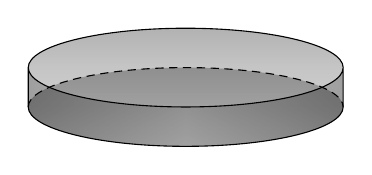
\begin{tikzpicture}
\fill[top color=gray!50!black,bottom color=gray!10,middle color=gray,shading=axis,opacity=0.25] (0,0) circle (2cm and 0.5cm);
\fill[left color=gray!50!black,right color=gray!50!black,middle color=gray!50,shading=axis,opacity=0.25] (2,0) -- (2,0.5) arc (360:180:2cm and 0.5cm) -- (-2,0) arc (180:360:2cm and 0.5cm);
\fill[top color=gray!90!,bottom color=gray!2,middle color=gray!30,shading=axis,opacity=0.25] (0,0.5) circle (2cm and 0.5cm);
\draw (-2,0.5) -- (-2,0) arc (180:360:2cm and 0.5cm) -- (2,0.5) ++ (-2,0) circle (2cm and 0.5cm);
\draw[densely dashed] (-2,0) arc (180:0:2cm and 0.5cm);
\end{tikzpicture}
\]


Using the fact that the disk is uniform, so mass density $\sigma$ is uniform
\[
M = \int \rho (\mathbf{x}) d\mathbf{x} = \int \rho(\mathbf{s}) d\mathbf{s} = \sigma \int r d\theta dr = \sigma \frac{1}{2} R^2 2\pi = \sigma \pi R^2
\]
\[
\sigma = \frac{M}{\pi R^2} = \text{ mass per unit area }
\]

\begin{equation}
I  = \int r^2 dm = \int r^2 \sigma r d\theta dr = \sigma \frac{1}{4} r^4 2\pi = \boxed{ \frac{MR^2}{2} }
\end{equation}

\end{enumerate}


\subsection{Euler's equations of motion, Euler's rotation equations}

In the body frame, inertia tensor $J \equiv I$ is time-independent.

\[
\begin{gathered}
\frac{d}{dt} \widehat{\Omega} - \text{ad}^*_{\widehat{\Omega}} \widehat{\Omega} = 0 
\end{gathered}
\]

Use (Eq. (4.36) Kambe (2009) \cite{TKambe2009}

\section{Waves}

\subsection{Signals, Fourier Analysis}

See Ch. 10 "Signals and Fourier Anaylsis" of Georgi (1992) \cite{Geor1992}.

\subsubsection{Example: A pulse on a String}

See 10.1.1 "A Pulse on a String", Sec. 10.1 "Signals in Forced Oscillation" of Georgi (1992) \cite{Geor1992}.

Consider transvere oscillation of a semiinfinite string stretched from $x=0$ to $x=\infty$, driven at $x=0$ with some arbitrary transverse signal $f(t)$, with a boundary condition at $\infty$ that there's no incoming traveling waves.

If given dispersion relation (10.1) of Georgi (1992) \cite{Geor1992}
\begin{equation}\label{Eq:NondispersiveDispersionRelation}
	\omega^2 = v^2 k^2
\end{equation}
This implies system that satisfies wave equation
\begin{equation}\label{Eq:NondispersiveWaveEquation}
	\frac{\partial^2}{\partial t^2} \psi(x,t) = v^2 \frac{\partial^2}{\partial x^2} \psi(x,t)
\end{equation}
((10.2) of Georgi (1992) \cite{Geor1992})

Its a mathematical fact that the general solution to Eq. \ref{Eq:NondispersiveWaveEquation} 
\begin{equation}
	\psi(x,t) = g(x- vt) + h(x+vt)
\end{equation}
where $g,h $ arbitrary. This fact is because of this straightforward derivation:

\[
\begin{aligned}
& \frac{\partial^2}{ \partial t^2} \psi(x,t) = v^2 (g''(x-vt) + h''(x+vt)) \\
&	\frac{\partial^2}{ \partial x^2} \psi(x,t) = g''(x-vt) + h''(x+vt)
\end{aligned}
\]

Boundary condition at $\infty$ implies $h=0$, because $h$ function describes wave moving in $-x$ direction. EY: by going to infinity, by physical intuition, we don't expect a reflection back from infinity.

Boundary condition at $x=0$ (substitute $x=0$ into $g$ and thus for $\psi$):
\begin{equation}
	g(-vt) = \psi(0,t) = f(t)
\end{equation}
((10.6) of Georgi (1992) \cite{Geor1992})

EY: Consider $\tau = t- \frac{x}{v}$:
\[
\begin{aligned}
	& g(-v\tau) = g(x-vt) \\
	& f(\tau) = f(t-\frac{x}{v})
\end{aligned}
\]

Thus we guess that 
\begin{equation}
	\psi(x,t) = f(t- \frac{x}{v})
\end{equation}
((10.7) of Georgi (1992) \cite{Geor1992})

e.g. 

\begin{equation}
	f(t) = \begin{cases} 1 - |t| & \text{ for } |t| \leq 1 \\
		0 & \text{for } |t| >1 \end{cases}
\end{equation}
((10.8) of Georgi (1992) \cite{Geor1992})

\subsubsection{Introduction to Fourier integrals}

The idea is to use linearity in a clever way. \\
We can take $f(t)$ apart into its component angular frequencies. \\
We already know how to solve forced oscillatio nproblem for each angular frequency. \\
\begin{itemize}
	\item Take individual solutions and add them back up. 
	\item The advantage of this is that it works for any dispersion relation, not just for Eq. \ref{Eq:NondispersiveDispersionRelation}.
\end{itemize}

\begin{equation}\label{Eq:FourierIntegral}
	f(t) = \int_{-\infty}^{\infty} d\omega C(\omega) e^{-i\omega t}
\end{equation}
((10.9) of Georgi (1992) \cite{Geor1992})

\begin{theorem}[Properties of Fourier integrals, coefficients]
In Eq. \ref{Eq:FourierIntegral}
\begin{equation}
	C(\omega) = C(-\omega)^*
\end{equation}
\end{theorem}

\begin{proof}
If $f(t) \in \mathbb{R}$, $f(t) = f^*(t)$ and so
\[
\begin{gathered}
	f(t) = \int_{-\infty}^{\infty} d\omega C(\omega) e^{-i\omega t} = f(t)^* = \int_{-\infty}^{\infty} d(\omega) C^*(\omega) e^{i\omega t} = \int_{\infty}^{-\infty} d(-\omega) C(-\omega)^* e^{-i\omega t} = \int_{-\infty}^{\infty} d(\omega) C(-\omega)^* e^{-i\omega t} \\
	\Longrightarrow C(\omega) = C(-\omega)^*
\end{gathered}
\]
\end{proof}

Since each frequency component of the force produces a wave traveling in $+x$ direction, we use linear superposition, and so we have
\[
\Longrightarrow \psi(x,t) = \int_{-\infty}^{\infty} d\omega C(\omega) e^{-i\omega t + ikx}
\]

\subsubsection{Dispersive Media, Group Velocity}

See 10.2.1 "Group Velocity", Sec. 10.2 "Dispersive Media and Group Velocity" of Georgi (1992) \cite{Geor1992}.

\subsubsection{Group Velocity}

You can send signals in a dispersive medium; the trick is to send the signal not directly as the function, $f(t)$, but as modulation of harmonic signal,
\begin{equation}
	f(t) = f_s(t) \cos{\omega_0 t}
\end{equation}
((10.17) of Georgi (1992) \cite{Geor1992}), where $f_s(t)$ is the signal. Very often, you want to do this anyway because the important frequencies in your signal, \\
$f_s(t)$, \\
may not match frequencies of the waves with which you want to send the signal, $\omega_0$ of $\cos{\omega_0 t}$. \\

Example: AM radio transmission, in which signal is derived from sound with a typical frequency of a few hundred cycles per second (Hz), but is carried as a modulation of amplitude of an electromagnetic radio wave, with frequency of a few million cycles per second ($\omega_0$).

Consider 
\[
\cos{ (k_+ x - \omega_+ t)} + \cos{ (k_- x - \omega_- t)} \equiv c(k_+ x - \omega_+ t) + c(k_- x - \omega_- t)
\]
Let $k_{\pm} = k_0 \pm k_s$, $\omega_{\pm} = \omega_0 \pm \omega_s$ for $k_s \ll k_0$, $\omega_s \ll \omega_0$.

Then
\begin{equation}\label{Eq:Example2TravelingWavesWithCarrierFrequency}
\begin{gathered}
	c(k_{\pm} x - \omega_{\pm}t) = c(k_{\pm} x) c(\omega_{\pm}t) + s(k_{\pm} x) s(\omega_{\pm} t) 
\end{gathered}
\end{equation}
and so for each term,
\[
\begin{gathered}
\begin{gathered}
	c(k_{\pm} x) c(\omega_{\pm} t) = c((k_0 \pm k_s) x) c((\omega_0 \pm \omega_s) t) = (c(k_0x) c(k_s x) \mp s(k_0x) s(k_s x)) (c(\omega_0 t) c(\omega_s t) \mp s(\omega_0 t) s(\omega_0 t)) = \\
= c(k_s x) c(\omega_s t)c(k_0x) c(\omega_0 t) \mp c(k_s x) s(\omega_s t) c(k_0 x) s(\omega_0t) \mp s(k_sx) c(\omega_s t) s(k_0x) c(\omega_0 t) + s(k_s x) s(\omega_s t) s(k_0x ) s(\omega_0 t) 
\end{gathered} \\
\quad \quad \\
\begin{gathered}
	s(k_{\pm}x) s(\omega_{\pm} t) = s(k_0 \pm k_s)x s(\omega_0 \pm \omega_s) t = (s(k_0x) c(k_sx) \pm c(k_0x) s(k_sx) ) (s (\omega_0 t) c(\omega_s t) \pm c(\omega_0 t) s(\omega_s t) ) = \\
	= c(k_s x) c(\omega_s t) s(k_0 x) s(\omega_0 t) \pm c(k_s x) s(\omega_s t) s(k_0x) c(\omega_0 t) \pm s(k_s x) s(\omega_0 t) c(k_0x) s(\omega_0 t) + s(k_s x) s(\omega_s t) c(k_0x) c(\omega_0 t)
\end{gathered}
\end{gathered}
\]
Terms with $\pm$ or $\mp$ in front cancel for when considering the total expression summing 2 terms in Eq. \ref{Eq:Example2TravelingWavesWithCarrierFrequency}, and so
\begin{equation}\label{Eq:SignalAndCarrierWavesAs2TravelingWaves}
\begin{gathered}
	\Longrightarrow 2 \cdot \left[ c(k_sx) c(\omega_s t) (c(k_0x - \omega_0t)) + s(k_s x) s(\omega_s t) c(k_0x - \omega_0t) \right] = 2 c(k_s x - \omega_s t) c(k_0x - \omega_0 t)
\end{gathered}
\end{equation}
((10.21) of Georgi (1992) \cite{Geor1992})

Since $k_s \ll k_0$, and $\omega_s \ll \omega_0$, so $c(k_s x - \omega_s t)$ varies slowly in $x$ and $t$ compared to second factor. You should think of this first factor as the signal in Eq. \ref{Eq:SignalAndCarrierWavesAs2TravelingWaves}. The second factor is called the \textbf{carrier wave}.

Then Eq. \ref{Eq:SignalAndCarrierWavesAs2TravelingWaves} describes a signal that moves with velocity
\begin{equation}
	v_s = \frac{ \omega_s }{k_s } = \frac{ \omega_+ - \omega_- }{ k_+ - k_- }
\end{equation}
((10.22) of Georgi (1992) \cite{Geor1992}) while smaller waves associated with second factor, carrier wave, move with velocity 
\begin{equation}
	v_0 = \frac{\omega_0}{k_0}
\end{equation}
((10.23) of Georgi (1992) \cite{Geor1992})

In limit as $k_+ - k_- = 2k_s$ becomes small, $v_s \equiv \frac{\omega_+ - \omega_- }{ k_+ - k_-} \mapsto \left. \frac{\partial \omega}{\partial k} \right|_{k=k_0}$.

$v_g = \left. \frac{\partial \omega}{ \partial k} \right|_{k=k_0}$ is called the "group velocity"; measures the speed the signal can actually be sent.

Suppose dispersion relation is slowly varying for some range of frequencies near some frequency $\omega_0$, 
\[
\begin{gathered}
	\omega = \omega(k) = \omega_0 + (k- k_0) \left. \frac{ \partial \omega}{ \partial k } \right|_{k=k_0} + \dots \\
	\omega_0 \equiv \omega(k_0)
\end{gathered}
\]
Higher order terms negligible only if $\Delta \omega \ll \omega_0$. If so let 
\[
\begin{gathered}
	\begin{gathered}
		\omega = vk + a \\
		k = \frac{\omega}{v} + b
	\end{gathered} \text{ \quad \, since \quad \, } \begin{gathered}
	a = \omega_0 - k_v \\
	b = -\frac{a}{v} = k_0 - \frac{ \omega_0}{v}
\end{gathered}
\end{gathered}
\]

$v$ is group velocity, $\left. v = \frac{\partial \omega}{ \partial k} \right|_{k=k_0}$

Send signal of form $f(t) e^{-i\omega_0 t}$ (modulate the amplitude by $f(t)$ that's non-zero for some range of frequencies, of carrier wave $e^{-i \omega_0 t}$):
\[
\begin{gathered}
	\psi(0,t) = f(t) e^{-i \omega_0 t} = \int_{-\infty}^{\infty} d\omega C(\omega) e^{-i\omega t} e^{-i\omega_0 t} = \int_{-\infty}^{\infty} d\omega C(\omega) e^{-i(\omega + \omega_0)t} = \int_{-\infty}^{\infty} d\omega C(\omega - \omega_0) e^{-i\omega t}
\end{gathered}
\]
where we used linearity or i.e. linear superposition or i.e. adding up frequency components for second equality, and $u= \omega + \omega_0$ substitution for 3rd equality.

Thus
\[
\psi(x,t) = \int_{-\infty}^{\infty} d\omega C(\omega - \omega_0) e^{-i\omega t} e^{ikx}
\]

For approximation $k = \frac{\omega }{v} + b$, 
\[
\begin{gathered}
\psi(x,t) = \int_{-\infty}^{\infty} d\omega C(\omega - \omega_0) e^{-i\omega t} e^{ i \left( \frac{\omega x}{v} + bx \right) } = \int_{-\infty}^{\infty} d\omega C(\omega - \omega_0) e^{ -i \omega \left( t - \frac{x}{v} \right) } e^{ibx } = \\
= \int_{-\infty}^{\infty} d\omega C(\omega) e^{-i (\omega + \omega_0) \left( t - \frac{x}{v} \right) } e^{ibx} = f(t - \frac{x}{v})	 e^{-i \omega_0 (t - \frac{x}{v} ) + ibx}
\end{gathered}
\]

Thus, for signal $f(t)$ s.t. $C(\omega) \approx 0$ for $| \omega - \omega_0| > \Delta \omega$, where $\Delta \omega \ll \omega_0$, \\
modulation $f(t)$ travels without change of shape at group velocity $v = \left. \frac{ \partial \omega}{ \partial k } \right|_{k=k_0}$. \\
Phase velocity $v_{\phi} = \frac{\omega}{k}$ has nothing to do with transmission of information, but notice because of $e^{ibx} = \exp{ \left( i \left( k_0 - \frac{ \omega_0}{v} \right) \right) }$ carrier wave travels at phase velocity
\[
\begin{gathered}
	\frac{ \omega_0 }{ b + \frac{\omega_0}{v} } = \frac{ \omega_0}{ k_0 - \frac{\omega_0}{v} + \frac{\omega_0}{v} } = \frac{\omega_0}{k_0} = v_{\phi}
\end{gathered}
\]

"You can see the difference between phase velocity and group velocity in your pool or bathtub by making a wave packet consisting of severla shorter waves." pp. 232, Sec. 10.2 of Georgi (1992) \cite{Geor1992}).

\subsubsection{Bandwidth, Fidelity, Uncertainty}

See Sec. 10.3 "Bandwidth, Fidelity, and Uncertainty" of Georgi (1992) \cite{Geor1992}.

\subsubsection{Inverse Fourier Transform}

Now suppose we have the inverse Fourier transform to be of this form:
\begin{equation}\label{Eq:InverseFourierTransform}
C(\omega) = \frac{1}{ 2\pi} \int_{-\infty}^{\infty} dt f(t) e^{i\omega t}
\end{equation}

Recall $f(t) = \int_{-\infty}^{\infty} d\omega C(\omega) e^{-i\omega t}$ of Eq. \ref{Eq:FourierIntegral}. 

Given $\frac{1}{2\pi}\int_{-\infty}^{\infty} dt f(t) e^{i\omega t}$ of Eq. \ref{Eq:InverseFourierTransform}, insert Eq. \ref{Eq:FourierIntegral} for $f(t)$:
\[
\begin{gathered}
	\frac{1}{2\pi} \int_{-\infty}^{\infty}dt \int_{-\infty}^{\infty} d\omega' C(\omega') e^{i (\omega- \omega')t} = \frac{1}{2\pi} \int_{-\infty}^{\infty} d\omega' C(\omega') \int_{-\infty}^{\infty} dt e^{i (\omega - \omega') t} 
\end{gathered}
\]
$\int_{-\infty}^{\infty} e^{ i(\omega - \omega') t} $ averages to zero unless $\omega' = \omega$.

Therefore $\frac{1}{2\pi} \int_{-\infty}^{\infty} dt f(t) e^{i\omega t} $ is proportional to $C(\omega)$.

Now consider $f(t) = e^{-\Gamma|t|}$.

\[
\begin{gathered}
	\int_{-\infty}^{\infty} dt e^{-\Gamma|t|} e^{i\omega t} =\int_0^{\infty} dt e^{t(i\omega - \Gamma)} + \int_{-\infty}^0 dt e^{i(i\omega + \Gamma) } = \left. \frac{ e^{t(i\omega - \Gamma)} }{ i\omega - \Gamma} \right|_0^{\infty} + \left. \frac{ e^{t(i\omega + \Gamma)} }{ i\omega + \Gamma} \right|_{-\infty}^0 = \frac{ i\omega + \Gamma}{ \omega^2 + \Gamma^2} + \frac{-i\omega + \Gamma}{ \omega^2 +\Gamma^2} = \frac{2\Gamma}{ \omega^2 + \Gamma^2}
\end{gathered}
\]
Note that for $\frac{1}{ i\omega - \Gamma}$, $\frac{1}{ i\omega + \Gamma}$, if $\omega = \mp i\Gamma$, there's a pole; otherwise $\forall \, \omega \in \mathbb{R}$, integral is well-behaved.

Then for this particular case $C(\omega) = \frac{1}{2\pi} \frac{ 2\Gamma}{ \omega^2 + \Gamma^2}$.

For $f(t) = e^{-\Gamma |t|}$, $f(0) = 1$. Then
\[
\int_{-\infty}^{\infty} d\omega C(\omega) e^{-i\omega t} = \int_{-\infty}^{\infty} d\omega \frac{1}{\pi} \frac{ \Gamma e^{-i\omega t} }{ \omega^2 + \Gamma^2} = \frac{1}{\pi} \int_{-\infty}^{\infty} \frac{d\omega \Gamma}{ \omega^2 + \Gamma^2} = \frac{1}{ \pi} \int_{-\pi/2}^{\pi/2} \frac{ \Gamma \sec^2{\theta} d\theta \Gamma}{ \Gamma^2 (\tan^2{\theta} + 1) } = 1
\]
So $\frac{1}{2\pi}$ factor is obtained.

In another way to get $C(\omega)$, the inverse Fourier transform, as the limit of a Fourier waves, consider $\psi(-\pi l,t) = \psi(\pi l,t) $, periodic boundary condition (notice the period is $2\pi l = T$), 
\[
\xrightarrow{ \text{ in general } } \psi(x) = \sum_{j=-\infty}^{\infty} c_j e^{-ijx/l}
\]
Notice that changing $c_j e^{-ijx/l}$ by $2\pi l$ just changes the phase of the exponential by some multiple of $2\pi$ and so each factor indeed obeys the periodic boundary condition.

Likewise, for $f(t)$, s.t. $f(-\pi T) = f(\pi T)$, $T$ large
\[
\begin{aligned}
	& f(t) = \sum_{j=-\infty}^{\infty} c_j e^{-ijt/T} \quad \quad \, \text{ (Fourier transform in time ) } \\
	& c_j = \frac{1}{2\pi T} \int_{-\pi T}^{\pi T} dt e^{ijt/T} f(t) 
\end{aligned}
\]

$\lim_{t\to \infty} f(t) = 0$, then $c_j \to 0$ as $T \to \infty$.  $\Longrightarrow \begin{aligned}
	& c_j T \to C(\omega) \\
	& j/T \to \omega 
\end{aligned}$, so then
\[
f(t) = \sum c_j e^{-ij t/T} = \sum (c_j T) e^{-ijt/T} \frac{1}{T} \to \int_{-\infty}^{\infty} d\omega C(\omega) e^{-i \omega t} 
\]
So we have these important results:
\begin{align}
	& \boxed{ f(t)  = \int_{-\infty}^{\infty} C(\omega) e^{- i\omega t}  }\\
	& \boxed{ C(\omega)  = \frac{1}{2\pi} \int_{-\infty}^{\infty} dt f(t) e^{ i \omega t}  }
\end{align}


\section{Fluid Mechanics, Fluid Flow}

\subsubsection{Courses to consider}

\href{https://ocw.mit.edu/courses/aeronautics-and-astronautics/16-01-unified-engineering-i-ii-iii-iv-fall-2005-spring-2006/fluid-mechanics/}{MIT 16.01, 16.02}

\subsubsection{Videos to watch}

\href{https://youtu.be/pAuQ4Hj2ZrU}{Engineering MAE 130A. Intro to Fluid Mechanics. Lecture 01.} UCI. Follow the rest of the videos.


\subsection{Buoyancy}

From Problem 1.3 of the Japan Physics Olympiad (2014) \cite{Japa2014}, Ch. 1, General Physics, Elementary Problems.

\problemhead{1.3} The part of the iceberg above the sea.
\[
\begin{aligned}
& \rho_{sw} = 1024 \, \text{kg}/m^3 \\
& \rho_{ice} = 917 \, \text{kg}/m^3
\end{aligned}
\]
with $sw \equiv$ sea water.

Find the ratio of the volume of the part of the iceberg above the sea to whole volume of the iceberg.

\solutionhead{1.3}

\textbf{The buoyancy force exerted on the iceberg is equal to the weight of the seawater displaced by the iceberg}.

\[
\begin{gathered}
	\rho_{sw} g V_{is} = \rho_{ice} gV_{ice} \Longrightarrow \frac{ \rho_{sw} }{ \rho_{ice}} = \frac{V_{ice}}{ V_{is}} 
\end{gathered}
\]
with iceberg in sea $\equiv$ is.

iceberg above sea $\equiv$ as
\[
\begin{gathered}
V_{as} / V_{ice} = \frac{V_{ice} - V_{is}}{ V_{ice}} = 1 - \frac{V_{is}}{V_{ice}} = 1 - \frac{ \rho_{ice}}{ \rho_{sw}} = 1 - \frac{917 \, \text{kg}/m^3}{ 1024 \, \text{kg}/ m^3 } = \frac{ 1024 - 917 }{ 1024} = \frac{107 } {1024} 
\end{gathered}
\]

\textbf{The buoyancy on a body equals the resultant force due to the pressure exerted by the surrounding fluid}, i.e.
\textbf{The buoyancy force exerted on a body (iceberg) is equal to the resultant force due to pressure exerted by the surrounding fluid (seawater)}.


Pressure on body of volume $V$ due to its surrounding fluid (whose density is $\rho$) acts perpendicularly to the boundary surface between the body and the fluid. 

Since fluid pressure at a deep location is greater than that at shallow location, resultant force due to pressure on boundary surface points upward. This resultant force is the buoyancy, $F$, acting on body. 

Consider region of fluid with same volume $V$ as body. \\

buoyancy $F \equiv$ force exerted vertically on body by its surrounding fluid $ \underbrace{ =}_{ \text{ balance gravitational force acting on} V }  \rho g V$ \\

For a body floating in a fluid, the magnitude of the buoyancy force acting on the body is equal to the magnitude of the gravitational force on the fluid displaced by the part of the body submerged in the fluid.

% https://tex.stackexchange.com/questions/341318/to-draw-a-diagram-like-this-what-code-do-i-need

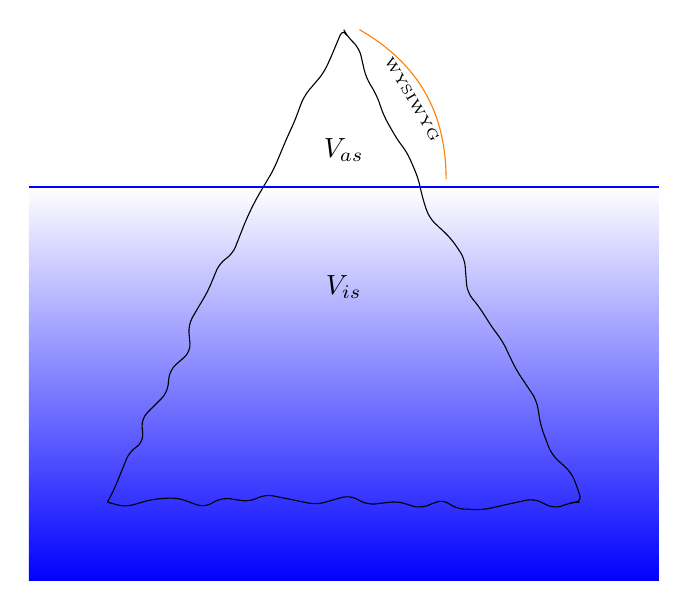
\begin{tikzpicture}

\fill [shade,
        top color=white,
        bottom color=blue] (-4,0) rectangle (4,-5);

\draw [decoration={random steps,segment length=0.3cm,amplitude=.1cm},
        decorate,
        rounded corners=.1cm]
     (-3,-4) -- (3,-4) -- (0,2) -- (-3,-4);


\draw [thick,blue] (-4,0) -- (4,0);

\node [above=2mm] at (0,0) {$V_{as}$};
\node [below=1cm] at (0,0) {$V_{is}$};

\draw [orange] (0.2,2) to[bend left] node[pos=0.5,sloped,below,font=\tiny,black] {WYSIWYG} (1.3,0.1);
\end{tikzpicture}

\subsection{Fluids as a State of Matter}

cf. Pert (2013) \cite{Pert2013}, Ch. 1 Introduction, 1.1 Fluids as a State of Matter.

fluid - isotropic, (no directional preference; identical values of a property in all directions), \\
locally homogeneous, macroscopic material, \\
whose particles are free to move within constraints established by the dynamical laws of continuum physics. \\
\emph{requirement that fluid be a continuum} - if volume of fluid successively subdivided into smaller elements, each element will remain structurally similar to its parent, and this subdivision can be carried out down to infinitesimal volumes. \\

\textbf{fluid particle} - fictitious particle fixed within fluid continuum and moving with flow velocity; \\
represents average over large number of microscopic particles. \\

\textbf{fluid point} - fixed in fluid moving with flow velocity; \\
- fluid particle always situated at same fluid point. \\

\textbf{infinitesimal volume} - within continuum of fluid, large compared with microscopic scales, but small compared with macroscopic ones. \\

fluid is made up of discrete microscopic particles, namely molecules, distributed randomly, with \\
distribution of velocities characteristic of fluid in termal equilibrium, typically Maxwell-Boltzmann distribution in a gas. \\

At typical experimental densities, \\
intermolecular separation extremely small and very much less than lab scale, i.e. $l_s \ll L_0$ \\
possible to average over small volumes which contain very large number of particles, yet very small on lab scale, $N-V$ in $V_0$, $V_0^{1/3} \ll L_0$ \\
$\Longrightarrow$ allow us to recover continuum approximation \\
obtain terms which characterize fluid as bulk material \\

Typical average quantities: \\
Density, $\rho$: number of mass particles per unit volume. \\
temperature, $\tau$: average energy of random motion per particle in thermal equilibrium \\
pressure $p$ average momentum flow associated with random motion per unit area. \\
flow velocity $u$ - mean velocity of molecules averaging out random motion. \\

role of collisions amongst particles important in defining irreversibility through loss of correlation between particles. \\

\emph{mean free path} $l_0$ - particles collide on average after distance equal to $l_0$ and time after collision interval\\

since fluid mechanics assumes fluid particles in thermal equilibrium and randomly distributed, this condition requires that spatial and temporal averages be taken to include large number of collisions; i.e. lab scale length $L_0$ large compared with $l_0$, and time to collision interval \\

effects of collisions on fluid transport (momentum and energy) are averaged over thermal distribution to yield bulk properties of material, namely viscosity and thermal conduction, respectively. \\

theory: flow of basic fluid may be calculated using Newtonian mechanics, classical thermodynamics, viscosity and thermal conductivity values. \\
Conditions under which this theory may be applied: \\
\begin{itemize}
	\item lab-scale lengths $L_0$ must be large compared with intermolecule separation and mean free path $l_0$ 
	\item characteristic lab times $T_0$ must be large compared with collision interval
	\item fluid locally in thermal equilibrium
\end{itemize}

cf. 1.2 The Fundamental Equations for Flows of a Dissipationless Fluid. Pert (2013) \cite{Pert2013}

\textbf{inviscid limit} - viscosity and thermal conduction are neglected \\
\textbf{adiabatic flow} - specific entropy of fluid particle constant in time \\
\textbf{isentropic flow} - specific entropy of each fluid particle has same initial value \\

many flows are both isentropic and adiabatic, e.g. ideal steady fluid flow, whose specific entropy an entry is everywhere constant.

\emph{Eulerian frame} - lab frame, coordinates fixed in space and time, derivatives are usual partial derivatives
\[
\left. \frac{ \partial }{ \partial t} \right|_{\mathbf{r}}, \, \left. \nabla \right|_t
\]
Consider coordinate system $(t, x^1, x^2, x^3)$ and so each vector field $\mathbf{e}_j$ forming basis of tangent space at each pt. expressed as linear combination of coordinate vector fields
\[
\left. \frac{\partial}{\partial t} \right|_{\mathbf{r}}, \, \left. \frac{\partial}{\partial x^1} \right|_{t}, \, \left. \frac{\partial}{\partial x^2} \right|_{t}, \, \left. \frac{\partial}{\partial x^3} \right|_{t},
\]

in Lagrangian frame, spatial variation seen by particle due to its motion is absorbed into time derivative:
\[
\frac{d}{dt} = \frac{\partial }{ \partial t} + \mathbf{v} \cdot \mathbf{\nabla} 
\]

Rather, consider total time derivative of integral of $n$-form: 
\[
\frac{d}{dt} \int_{V_0} \omega = \int_{V_0} \mathcal{L}_{\frac{\partial}{\partial t} + \mathbf{v} } \omega 
\]

Volume form $\Omega^n(M) = \bigwedge^n (T^*M)$
\[
\text{vol}^n \in \Gamma(\Omega^n(M)) = \Gamma(\bigwedge^n T^*M)
\]
i.e. $\text{vol}^n$ is $n$-form, a section of the line bundle, $\Omega^n(M) = \bigwedge^n T^*M$

Now
\[
\text{vol}^n = \frac{\sqrt{g}}{ n!} \epsilon_{i_1, \dots i_n} dx^{i_1} \wedge \dots \wedge dx^{i_n}
\]

Consider 
\[
\text{vol}^{n+1} = \frac{\sqrt{g}}{ (n+1)!} \epsilon_{i_0 i_1, \dots i_n} dx^{i_0} \wedge dx^{i_1} \wedge \dots \wedge dx^{i_n}
\]

\subsection{Lagrangian frame}

cf. Pert (2013) \cite{Pert2013} 1.3 Lagrangian Frame.

\textbf{Lagrangian frame} - frame of the moving particle; \\
Lagrangian reference frame considers fluid from point of view of an observer on a fluid particle. \\

fluid particle may be conveniently identified by coordinate set, which is fixed on the particle, \\
$\mathbf{\Lambda} = (\lambda, \mu, \nu)$ i.e. triad of numbers. \\
e.g. $\mathbf{\Lambda}$ maybe initial position of particle $\mathbf{r}_0 = (x_0, y_0, z_0)$, i.e. fluid particle labeled by some (time-independent) vector field $\mathbf{x}_0 \equiv \mathbf{\Lambda}$. \\

$\Longrightarrow $ position, velocity, thermodynamic state of particles are therefore functions of time alone. \\
$\Longrightarrow$ leads to simple set of kinematic and dynamic relations governing motion of particle \\
\[
\begin{gathered}
	\mathbf{r} = \mathbf{r}(t) = (x(t), y(t), z(t)) = (x^1(t), x^2(t), x^3(t)) \\ 
	\dot{ \mathbf{r}} \equiv \dot{\mathbf{r}}(t) \equiv \frac{d\mathbf{r}}{dt} \equiv \frac{d\mathbf{r}}{dt} (t) = \mathbf{v} \equiv \mathbf{v}(t)
\end{gathered}
\]
or 
\begin{equation}
\begin{gathered}
\frac{d\mathbf{r}}{dt} = \mathbf{v} \\ 
\frac{d\mathbf{v}}{dt} = \frac{\mathbf{F}}{m}
\end{gathered}
\end{equation}
cf. Eq. (1.2) of Pert (2013) \cite{Pert2013}, i.e. \\

flow described by function $\mathbf{X}(\mathbf{x}_0, t)$ giving position of particle labeled at $\mathbf{x}_0$ at time $t$.

\subsection{Momentum conservation in Lagrangian Frame-Euler's Equation}

Recall that a connection $\nabla$ on smooth manifold $(M, \mathcal{O}, \mathcal{A})$ is a map that takes a pair consisting of a vector (field) $X$ and $(p,q)$-tensor field $T$ and sends them to a $(p,q)-$ tensor (field) $\nabla_XT$, i.e. 
\[
\nabla : \mathfrak{X}(M) \times (\otimes^p TM \otimes^q T^*M) \to \otimes^p TM \otimes^q T^*M
\]
s.t. 
\[
\begin{aligned}
& \nabla_X f = Xf \quad \, \forall \, f \in C^{\infty}(M) \\ 
& \nabla_X(T + S) = \nabla_X T + \nabla_X S \\ 
& \nabla_X(T(\omega, Y)) = (\nabla_X T)(\omega, T) + T(\nabla_X \omega, Y) + T(\omega, \nabla_X Y) \\
& \nabla_{fX + Z} T = f\nabla_X T + \nabla_Z T , \quad \, f \in C^{\infty}(M) \quad \, \text{ "Leibnitz" rule }
\end{aligned}
\]
cf. Schuller, International Winter School on Gravity and Light held central lectures.

Remember that in the Lagrangian frame, we are an observer following an individual fluid parcel or i.e. "fluid particle" as it moves through space and time. This fluid particle will obey Newton's 2nd. law: $\nabla_{u} u = \frac{F}{m} \Longleftrightarrow m \cdot \mathfrak{a} = F$. 

\[
\begin{gathered}
\nabla_u u = \nabla_{u^{\mu}\frac{\partial}{\partial x^{\mu}}} (u^{\nu} \frac{\partial}{\partial x^{\nu}}) = u^{\mu} \nabla_{\frac{ \partial }{\partial x^{\mu}} } (u^{\nu} \frac{ \partial }{ \partial x^{\nu}}) =  u^{\mu} \left( \nabla_{\frac{ \partial }{\partial x^{\mu}} } u^{\nu} \right) \frac{ \partial }{ \partial x^{\nu}} + u^{\mu} u^{\nu} \nabla_{\frac{ \partial }{\partial x^{\mu}} }  \frac{ \partial }{ \partial x^{\nu}} = \\
	= u^{\mu} \frac{ \partial u^{\nu} }{ \partial x^{\mu}} \frac{\partial}{\partial x^{\nu}} + u^{\mu}u^{\nu} \Gamma^{\gamma}_{\mu \nu} \frac{\partial}{\partial x^{\gamma}}
	\end{gathered}
	\]

Let $u^0 = 1$.
\[
\begin{gathered}
\nabla_u u = \frac{\partial u^a}{\partial t} \frac{\partial }{ \partial x^a} + u^b \frac{\partial u^a}{\partial x^b} \frac{\partial}{\partial x^a} + u^{\mu} u^{\nu} \Gamma^a_{\mu \nu} \frac{\partial}{\partial x^a}
\end{gathered}
\]
where $\Gamma^0_{ba} = 0$ since $\nabla dt =0$ and we choose a stratified atlas $\mathcal{A}_{\text{stratified}}$.

Then let
\[
\int \rho \text{vol}^n \nabla_u u = F_{\text{tot}}  = \int f^i \text{vol}^n \otimes e_i
\]

From Sec. 2.4 Equations of Motion Neglecting Viscosity, pp. 38, Sabersky, et. al. (1998) \cite{SAHG1998}, the principal forces are those due to pressures acting on surfaces and to forces acting directly on a mass of the particle:
\[
\begin{gathered}
\int_{\partial V} p dS^i \otimes e_i = \int_V \mathbf{d} (pdS^i \otimes e_i) = \int_V \frac{\partial p}{\partial x^j} dx^j \wedge \left( \frac{\sqrt{g}}{(n-1)!} \epsilon^i_{\, i_2, \dots i_n} dx^{i_2} \wedge \dots \wedge dx^{i_n} \right) \otimes e_i = \\
\int_V \frac{\partial p}{\partial x^j} g^{ij} \text{vol}^n \otimes e_i = \int_V (\text{grad}p)^i \text{vol}^n \otimes e_i \\
\Longrightarrow \int \rho \text{vol}^n \nabla_u u = -\int_V (\text{grad}p)^i \text{vol}^n \otimes e_i + \int_V f^i \text{vol}^n \otimes e_i
\end{gathered}
\]
\begin{equation}\label{Eq:EulerianEquationMomentumConservationFluidFlow}
\begin{gathered}
\Longrightarrow \rho (\nabla_u u)^i = -(\text{grad}p)^i + f^i \\
(\nabla_u u)^i = -\frac{1}{\rho} (\text{grad}p)^i + f^i
\end{gathered}
\end{equation}
describes the motion of a perfect fluid.

Assuming a non-rotating, inertial frame (so that we can set the Christoffel symbols to 0),
\begin{equation}\label{Eq:EulerianEquationMomentumConservationFluidFlowInertialFrame}
\frac{\partial}{\partial t} u^i + u^b \frac{\partial u^i}{\partial x^b} = - \frac{1}{\rho}(\text{grad}p)^i + f^i
\end{equation}
which describes the motion of the perfect fluid in an inertial ref. frame. Compare this to Eqns. (2.10a- 2.10c) of Sabersky (1998) \cite{SAHG1998}. Sabersky says that no assumptions were made about density so these results apply to compressible fluid as well as incompressible ones. Also Eqns. \ref{Eq:EulerianEquationMomentumConservationFluidFlow}, \ref{Eq:EulerianEquationMomentumConservationFluidFlowInertialFrame} are called either Euler's Equation by Pert (2013) \cite{Pert2013} or Eulerian equation by Sabersky, et. al. (1998) \cite{SAHG1998}



\subsection{Mass Conservation for Fluid Flow, Continuum media}

The mass of fluid in some volume $V_0 \subset N$ is $\int_{V^0} \rho \text{vol}^n$, where $\rho$ is fluid density, $\rho \in C^{\infty}(N)$.  

The total mass of fluid flowing out of volume $V_0$ is 
\[
\begin{gathered}
\frac{d}{dt} \int_{V_0} \rho \text{vol}^n = \int_{V_0} \mathcal{L}_{\frac{\partial}{\partial t} + \textbf{u}} (\rho \text{vol}^n) = \int_{V_0} \frac{ \partial }{\partial t} \rho \text{vol}^n + \int_{V_0} \mathcal{L}_u \rho \text{vol}^n   \\
\int_{V_0} \mathcal{L}_u \rho \text{vol}^n = \int_{V_0} di_{\mathbf{u}} \rho \text{vol}^n  + i_{\mathbf{u}} d\rho \text{vol}^n = \int_{V_0} di_{\mathbf{u}} \rho \text{vol}^n + 0 = \int_{V_0} di_{\mathbf{u}} \rho \text{vol}^n = \int_{\partial V_0} i_{\mathbf{u}} \rho \text{vol}^n
\end{gathered}
\]  
Now
\[
\begin{gathered}
i_u \text{vol}^n = i_u\frac{\sqrt{g}}{n!} \epsilon_{i_1 \dots i_n} dx^{i_1} \wedge \dots \wedge dx^{i_n} \\ 
i_u dx^{i_1} \wedge \dots \wedge dx^{i_n} = u^{i_1} dx^{i_2} \wedge \dots \wedge dx^{i_n} - dx^{i_1} \wedge u^{i_2} dx^{i_3} \wedge \dots \wedge dx^{i_n} +  \dots + (-1)^{n+1} dx^{i_1} \wedge \dots \wedge dx^{i_{n-1}} u^{i_n} = \epsilon^{i_1 \dots i_n}_{j_1 \dots j_n } u^{j_1 } dx^{j_2} \wedge \dots \wedge dx^{j_n}  
\end{gathered} 
\]
\begin{equation}\label{Eq:TimeIndependentMassVolumeTerm}
\Longrightarrow i_u\text{vol}^n = \frac{ \sqrt{g}}{ (n-1)!} \epsilon_{j_1 \dots j_n} u^{j_1} dx^{j_2} \wedge \dots \wedge dx^{j_n}
\end{equation}

We can also rewrite Eq. \ref{Eq:TimeIndependentMassVolumeTerm} to be a "surface differential":
\begin{equation}
\begin{gathered}
\int_{V_0} \mathbf{d}i_{\mathbf{u}} \rho \text{vol}^n = \int_{\partial V_0} i_{\mathbf{u}} \rho \text{vol}^n = \\
\int_{\partial V_0} \rho \frac{ \sqrt{g}}{ (n-1)!} u^{j_1} \epsilon_{j_1 j_2 \dots j_n} dx^{j_2} \wedge \dots \wedge dx^{j_n} \equiv \int_{\partial V_0} \rho \mathbf{u} \cdot d\mathbf{S} \equiv \int_{\partial V_0} \rho \langle \mathbf{u}, d\mathbf{S} \rangle 
\end{gathered}
\end{equation}


If $\sqrt{g} = 1$, $n=2$, 
\[
i_u \text{vol}^2 = (u^1 dx^2 - u^2 dx^1) = u\cdot n_1 dx^2 + u\cdot n_2 dx^1 = u\cdot n dS
\]
with $n_1 =e_1$ and $n_2=-e_2$.  

Now 
\[
\begin{gathered}
di_u \rho \text{vol}^n = \\
= \frac{ \partial ( \sqrt{g} \rho u^{j_1} ) }{ \partial x^k} \frac{ \epsilon_{j_1 \dots j_n} }{ (n-1)! } dx^k \wedge dx^{j_2} \wedge \dots \wedge dx^{j_n} = \frac{ \partial (\sqrt{ g} \rho u^k) }{ \partial x^k} \frac{ \epsilon_{j_1 \dots j_n }}{ n!} dx^{j_1} \wedge \dots \wedge dx^{j_n} = \frac{1}{\sqrt{g}} \frac{ \partial (\sqrt{g} \rho u^k)}{ \partial x^k} \text{vol}^n = \\
= \frac{ \partial (\rho u^k)}{ \partial x^k} \text{vol}^n + \rho u^k \frac{ \partial \ln{ \sqrt{g}}}{ \partial x^k} \text{vol}^n = \text{div}(\rho u) \text{vol}^n + \rho u^k \frac{ \partial \ln{ \sqrt{g}}}{ \partial x^k} \text{vol}^n
\end{gathered}
\]
Now if $\sqrt{g}=1$, then 
\[
\begin{gathered}
\frac{d}{dt} \int_{V_0} \rho \text{vol}^n = \int_{V_0} \frac{ \partial \rho }{ \partial t} \text{vol}^n + \int_{V_0} di_u \rho \text{vol}^n = \int_{V_0} \frac{ \partial \rho }{ \partial t} \text{vol}^n + \int_{V_0} \text{div}(\rho u) \text{vol}^n \Longrightarrow \frac{ \partial \rho}{\partial t} + \text{div}(\rho u) = 0
\end{gathered}
\]
which is the so-called mass continuity equation.  $ j = \rho u$ is the mass flux density.  

Thus,

\begin{equation}\label{Eq:MassConservationForContinuum}
\begin{gathered}
\text{(mass conservation)} \\
m = m(t) := \int_{V_0} \rho \text{vol}^n, \, V_0 \subset N \\
\dot{m} \equiv \frac{d}{dt}m(t) = \int_{V_0} \left( \frac{\partial \rho }{ \partial t} \text{vol}^n + \mathbf{d}i_{\mathbf{u}} \rho \text{vol}^n \right) = \boxed{ \int_{V_0} \frac{ \partial \rho }{ \partial t} \text{vol}^n + \int_{\partial V_0} \rho \mathbf{u} \cdot d\mathbf{S} } \\
\text{ if } \sqrt{g} = 1, \text{ and } \dot{m} = 0, \text{ then } \\
\frac{\partial \rho }{ \partial t} + \text{div}(\rho \mathbf{u}) = 0 
\end{gathered}
\end{equation}

Sec. 1.4 Eulerian Frame, 1.4.1 Conservation of Mass-Equation of Continuity, pp. 8 of Pert (2013) \cite{Pert2013} says that Eq. \ref{Eq:MassConservationForContinuum} is for the Eulerian Frame.

From \href{https://en.wikipedia.org/wiki/Lagrangian_and_Eulerian_specification_of_the_flow_field}{wikipedia}, recall that the \emph{Eulerian specification} focuses on specific locations in space through which fluid flow as time passes. Visualize by sitting on bank of river and watch water pass fixed location. In the Eulerian specification of field, field represented as a function of position $\mathbf{x}$, time $t$, e.g. $\mathbf{u}(\mathbf{x}, t) \equiv $ flow velocity.




TODO: 20190804 Frankel (2012) \cite{TFrankel2012} in pp. 138 and onwards, for Sec. 4.3. Differentiation of Integrals posed the rightful question, "How does one compute the rate of change of an integral when the domain of integration is also changing?" Revisit the derivation from a Lie derivative and 1-parameter flow point of view.

Force should not be represented by a vector but rather by a 1-form. Then, 
\[
f \in \Omega^1(N), \, f=f(t, \mathbf{x}) = f_j dx^j \, \, j=1, \dots n , \, \mathbf{x} = (x^1, \dots x^n), \, \text{dim}N = n
\]
Indeed, the reason for $f$ to be a 1-form is that we integrate differential forms, we don't integrate vectors. 

\begin{equation}
W = \int_C f \qquad \, \text{(line integral)}
\end{equation}

\emph{If} $f$ conservative, $\exists\, $ scalar $U = U(x)$; $x\in N$ s.t. $f=-dU$.

Let $\mathbf{u} = u^j(t,\mathbf{x}) \frac{\partial}{ \partial x^j} \in \mathfrak{X}(N)$ generate flow $\phi_t$.

The Lie derivative along vector field $\mathbf{u}$, $\mathcal{L}_{\mathbf{u}}$, can be calculated in at least 2 ways: from the definition:
\[
\mathcal{L}_{\mathbf{u}} \omega  =\frac{d}{dt} \left. \right|_{t = 0} \phi_t^*\omega
\]
or Cartan's magic formula:
\begin{equation}
\begin{gathered}
	\mathcal{L}_{\mathbf{u}} \text{vol}^n = (i_{\mathbf{u}}\mathbf{d} + \mathbf{d}i_{\mathbf{u}}) \text{vol}^n = 0 + \mathbf{d}i_{\mathbf{u}} \text{vol}^n = \mathbf{d}i_{\mathbf{u}} \left( \frac{ \sqrt{g}}{n!} \epsilon_{i_1 \dots i_n} dx^{i_1} \wedge \dots \wedge dx^{i_n} \right) = \\ 
	= \mathbf{d} \left( \frac{\sqrt{g}}{(n-1)! } \epsilon_{j_1 \dots j_n} u^{j_1} dx^{j_2} \wedge \dots \wedge dx^{j_n} \right) = \frac{ \partial (\sqrt{g} u^{j_1} )}{ \partial x^k} \frac{ \epsilon_{j_1 \dots j_n}}{(n-1)!} dx^k \wedge dx^{j_2} \wedge \dots \wedge dx^{j_n} = \\
	= \frac{ \partial (\sqrt{g} u^{j_1}) }{ \partial x^k} \frac{ \epsilon_{j_1 \dots j_n} }{ (n-1)! } \epsilon^{k j_2 \dots j_n}_{ k_1, \dots, k_n} dx^{k_1} \wedge \dots \wedge dx^{k_n} \underbrace{\left( \frac{ \sqrt{g}}{ \sqrt{g}} \right)}_{=1} = \frac{1}{\sqrt{g}} \frac{ \partial ( \sqrt{g} u^k) }{ \partial x^k} \text{vol}^n =  \\
	= (\text{div}{\mathbf{u}}) \text{vol}^n
\end{gathered}
\end{equation}
cf. \url{https://math.stackexchange.com/questions/2566381/lie-derivative-of-volume-form?rq=1}

Note that
\[
\begin{gathered}
	\text{div}: \mathfrak{X}(N) \to C^{\infty}(N) \\ 
 \mathcal{L}_{\mathbf{u}}: \Omega^n(N) \to \Omega^n(N) 
\end{gathered}
\]

Frankel (2012) \cite{TFrankel2012} on pp. lvii of the "Elasticity and Stresses" section offered this analogy: "While work in particle mechanics pairs a force covector ($f_i$) with a contravariant tangent vector ($dx^i/dt$) to a curve, work done by traction in elasticity pairs the contravariant stress force 2-form $\mathcal{S}$ with the covector valued deformation 1-form $\mathcal{E}$, to yield a scalar valued 3-form.

Instead of pushing along a curve (line) particle to do work, what does it mean to do work on a moving fluid element? One could possibly try to consider the deformation of a volume element under fluid flow. Frankel (2012) \cite{TFrankel2012} in Sec. 4.2. The Lie Derivative of a Form, on pp. 132, asks "If a flow deforms some attribute, say volume, how does one measure the deformation? $\mathcal{L}_{\mathbf{u}}\text{vol}^n$ "is the $n$-form that reads off the rate of change of volume of a parallelopiped spanned by $n$ vectors that are pushed forward by the flow $\phi_t$." So, "in other words, $\mathcal{L}_{\mathbf{u}}\text{vol}^n$ \emph{measures how volumes are changing under the flow} $\phi_t$ \emph{generated by} $\mathbf{X}$" on pp. 133 on Frankel (2012) \cite{TFrankel2012}. 

Then rate of work done on a fluid element could be the following:

\[
\begin{gathered}
W = \int_V \mathcal{L}_{\mathbf{u}}(p \text{vol}^n) = \int_V \mathbf{d} i_{\mathbf{u}} p \text{vol}^n = \int_{\partial V} i_{\mathbf{u}} p \text{vol}^n = \int_{\partial V} p \mathbf{u} \cdot d\mathbf{S} 
\end{gathered}
\]

TODO: work on a fluid element?

\subsection{Bernoulli's equation}

\subsubsection{Simple cases}

cf. Ch. 3 The Bernoulli Equation, Sec. 3.2 "A Simple Form of the Bernoulli Equation", pp. 90, Sabersky, et. al. (1998) \cite{SAHG1998}


Start from Eq. \ref{Eq:EulerianEquationMomentumConservationFluidFlow}. So
\[
(\nabla_u u)^i = \frac{-1}{\rho} (\text{grad}p)^i + f^i
\]
Suppose $f^i=0$ (no external forces), $\frac{\partial u^i}{\partial t} = 0$ (steady flow). Suppose $\Gamma^a_{\mu \nu} =0$ (Cartesian coordinates? TODO: find out the conditions when this is true).

Suppose the flow is irrotational (TODO: find out the condition for irrotational flow; is it when having streamlines or ?). For the curl, recall that an external derivative $\mathbf{d}$ takes a 1-form into a 2-form. So consider
\[
\begin{gathered}
 \mathbf{u} \in \mathfrak{X}(V), \mathbf{u} \xrightarrow{\flat} u_i dx^i = g_{ij} u^j dx^i \\ 
 d\mathbf{u}^{\flat} \in \Omega^2(V), \, \mathbf{d}\mathbf{u}^{\flat} = \frac{\partial u_j}{\partial x^i} dx^i \wedge dx^j = \frac{ \partial (g_{ij} u^j) }{\partial x^a} dx^a \wedge dx^i
\end{gathered}
\]
If we have the condition that the flow is irrotational, i.e. 
\begin{equation}
\mathbf{d}\mathbf{u}^{\flat} = 0
\end{equation}
then
\[
\begin{gathered}
	\mathbf{d}\mathbf{u}^{\flat} (\mathbf{u}) = \frac{\partial (u_i) }{ \partial x^a} u^a dx^i - \frac{\partial (u_i) }{ \partial x^a} dx^a u^i = 0 \Longrightarrow u^a \frac{ \partial (u_i) }{ \partial x^a} dx^i = u^i \frac{\partial u_i}{ \partial x^a} dx^a
\end{gathered}
\]

%So if $g_{ij}$ is position independent, then
%\begin{equation}\label{Eq:MagnitudeOfVectorTransportForIrrotationalFlow}
%u^a \frac{\partial u_i}{\partial x^a} dx^i = u^i \frac{\partial u_i}{\partial x^a} dx^a 
%\end{equation}
%One must be aware that Eq. \ref{Eq:MagnitudeOfVectorTransportForIrrotationalFlow} necessarily depends on having the Christoffel symbols $\Gamma^a_{\mu \nu}$ be zero, the metric be position-independent, and the flow be irrotational.

Take the exterior derivative $\mathbf{d}$ of the inner product of a vector with itself in the most general case on a metric manifold:
\[
\begin{gathered}
d(u_i u^i) = d(g_{ij} u^j u^i) = \frac{ \partial g_{ij} }{ \partial x^k} u^j u^i dx^k  + g_{ij} \frac{ \partial u^j}{ \partial x^k} u^i dx^k + g_{ij} u^j \frac{\partial u^i}{\partial x^k} dx^k = \\
= 2 u_j \frac{ \partial u^j}{\partial x^k} dx^k + u^i u^j \frac{\partial g_{ij}}{\partial x^k} dx^k 
\end{gathered}
\]


Since the Christoffel symbols are the connection coefficients of a \emph{metric-compatible} affine connection (i.e. they can be used to construct a connection $\nabla$ s.t. $\nabla g = 0$), then \footnote{ \href{https://physics.stackexchange.com/questions/175235/prove-christoffel-symbol-identity}{"Prove Christoffel Symbol Identity", Physics StackExchange}}

\begin{equation}
\nabla_i g_{jk} = \frac{ \partial g_{jk}}{\partial x^i} - \Gamma^s_{ji} g_{sk} - \Gamma^s_{ki} g_{js} = 0
\end{equation}
and so
\begin{equation}
\begin{gathered}
 u^i u^j \frac{ \partial g_{ij}}{\partial x^k} = u^i u^j \left[ \Gamma^s_{ik} g_{sj} + \Gamma^s_{jk} g_{is} \right] = u^i u_s \Gamma^s_{ik} + u_s u^j \Gamma^s_{jk} = 2u_s u^i \Gamma^s_{ik}
\end{gathered}
\end{equation}

%One must be aware that Eq. \ref{Eq:MagnitudeOfVectorTransportForIrrotationalFlow} necessarily depends on having the Christoffel symbols $\Gamma^a_{\mu \nu}$ be zero, the metric be position-independent, and the flow be irrotational.

Then 
\begin{equation}\label{Eq:ExteriorDerivativeOfMagnitudeSquareOfVector}
\begin{gathered}
\frac{1}{2} \mathbf{d}(u^2) = u_j \frac{ \partial u^j}{\partial x^k} dx^k + u_s u^i \Gamma^s_{ik} dx^k
\end{gathered}
\end{equation}

Eq. \ref{Eq:ExteriorDerivativeOfMagnitudeSquareOfVector} only depended upon the fact that the connection $\nabla$ is \emph{metric-compatible}.

So if we suppose that the Christoffel symbols $\Gamma^s_{ik}$ are 0, and have irrotational flow, as well,
\[
\begin{gathered}
\mathbf{d}(u^2 / 2) = u_j \frac{\partial u^j}{ \partial x^k} dx^k  + 0 = u^a \frac{ \partial u_i}{\partial x^a} dx^i 
\end{gathered}
\]

Now consider the RHS of Eq. \ref{Eq:EulerianEquationMomentumConservationFluidFlow}, with $f_i =0$,
\[
\begin{gathered}
	\frac{-1}{\rho} (\text{grad}{p})^i \xrightarrow{ \flat} \frac{-1}{\rho} (\text{grad}p)^i g_{ij} dx^j = \frac{-1}{\rho}  \frac{\partial p}{\partial x^k} g^{ki} g_{ij} dx^j = \frac{-1}{\rho} \frac{ \partial p}{\partial x^j} dx^j = \frac{-1}{\rho} \mathbf{d}p
\end{gathered}
\]
So if the fluid is incompressible, then $\rho$ is constant and so we can write

\begin{equation}
\mathbf{d} \left( \frac{u^2}{2} + \frac{p}{\rho} \right) = 0 
\end{equation}
for any irrotational, incompressible, fluid flow with no (external) body forces.

\subsubsection{Venturi tube example}

cf. Example 3.1 in Sabersky, et. al. (1998) \cite{SAHG1998}

Consider flow of liquid through the tube shown. Determine pressure difference between points 1 and 2 as a function of flow rate $Q$, density $\rho$. Velocity assumed constant over cross sections, and pressure will also be assumed uniform over each of these 2 areas $A_1$, $A_2$. Also assume there's no viscosity. 

\solutionhead{Example 3.1 in Sabersky, et. al. (1998) \cite{SAHG1998}}

Since density is constant, continuity equation requires that for $Q$ the volume flow rate,
\[
\text{flow rate} Q = u_1 A_1 = u_2 A_2
\]

\[
\begin{gathered}
	\frac{u_1^2}{2} + \frac{p_1}{\rho_1} = \frac{u_2^2}{2} + \frac{p_2}{\rho_2} \Longrightarrow \begin{aligned} & \quad \\ 
	& \frac{Q^2}{2A_1^2} + - \frac{Q^2}{2A_2^2} = \frac{ -(p_1- p_2) }{\rho}  \\
	& \frac{Q^2}{2} \left( \frac{1}{A_1^2} - \frac{1}{A_2^2} \right) = \frac{-(p_1 - p_2) }{\rho} \end{aligned} \text{ or } 
p_1 - p_2 = \frac{ + \rho Q^2}{2A_2^2} \left( 1 - \frac{A_2^2}{A_1^2} \right) 
\end{gathered}
\]

\subsubsection{Conservative body forces with Bernoulli equation}

cf. Sec. 3.3 in Sabersky, et. al. (1998) \cite{SAHG1998}

Consider $U= U(x)$, force potential. 

\[
\begin{gathered}
	-\mathbf{d}U = \frac{ - \partial U}{\partial x^i} dx^i = f_i dx^i \\
 \mathbf{d}\left( \frac{u^2}{2} + \frac{p}{\rho} + U \right) = 0 
\end{gathered}
\]

\subsubsection{Barotropic Fluids ($\rho = \rho(p)$) with Bernoulli equation}

cf. Sec. 3.4 in Sabersky, et. al. (1998) \cite{SAHG1998}

\emph{Barotropic fluid}: density is single-valued function of $p$. In the absence of heat transfer and absence of entropy change, by thermodynamics this can be shown to be barotropic.

\[
\begin{gathered}
\mathbf{d} \left( \frac{u^2}{2} \right) = -\frac{1}{\rho} \mathbf{d}p - \mathbf{d}U \text{ or } \mathbf{d} \left( \frac{u^2}{2} + U \right) + \frac{1}{\rho} \mathbf{d}p
\end{gathered}
\]

Suppose $i=i(p)$ s.t. $di = \frac{\partial i}{\partial p} dp = \frac{1}{\rho (p)} = \frac{di}{dp} dp$. So
\[
\begin{gathered}
\frac{di}{dp} = \frac{1}{\rho(p)} \text{ or } i = \int \frac{1}{\rho} dp + \text{ const } \\
\Longrightarrow \mathbf{d} \left( \frac{u^2}{2} + U + i \right) = 0 
\end{gathered}
\]

In special case of isentropic flow of perfect gas, $\frac{P}{\rho^{\nu}} = $ const. and $ i =\int \frac{dp}{p^{1/\nu}} = \frac{kp^{1-1/\nu}}{1- 1/\nu} = $ enthalpy.

\subsubsection{Nonsteady flow $\frac{\partial u}{\partial t}$ with Bernoulli equation}

First, use the musical isomorphism to transform the (1,0) tensor:
\[
\begin{gathered}
\frac{ \partial u^i}{\partial t}\frac{\partial}{\partial x^i} \xrightarrow{\flat} g_{ij} \frac{\partial u^i}{\partial t} dx^j
\end{gathered}
\]

Along a curve $\begin{aligned} & \quad \\ 
& \gamma = \gamma^i(t) = x^i(t) \text{ s.t. } \\
& \dot{\gamma} = \dot{\gamma}^i(t) \frac{ \partial}{\partial x^i} = u^i(t, \gamma(t)) \frac{\partial}{\partial x^i}
\end{aligned}$. Then

\[
\begin{gathered}
\int_{\gamma} g_{ij} \frac{\partial u^i}{\partial t} dx^j = \int g_{ij} \frac{\partial u^i}{\partial t} \dot{\gamma}^j(t) dt = \int g_{ij} \frac{\partial u^i}{\partial t} u^j dt = \int \frac{\partial \| u \| }{ \partial t} dt 
\end{gathered}
\]
The last step can be made only if the metric $g$ is time-independent.

cf. Example 3.2 in Sabersky, et. al. (1998) \cite{SAHG1998}. 

Consider the \emph{efflux} of liquid of density $\rho$ through an orifice of area $A_0$ at the bottom of a large tank of cross-sectional area $A_t$. \\
The depth of liquid at the given instant is $y$. \\
pressure exerted on the liquid in the tank is maintained at $p_t$, \\
pressure outside the orifice is the atmospheric pressure $p_a$. \\

The action of gravity is to be considered, but frictional effects may be neglected. Velocity of efflux $u_j$ is to be determined for these conditions. \\

efflux - something given off in or as if in a stream (Webster dictionary)

\solutionhead{Example 3.2 in Sabersky, et. al. (1998) \cite{SAHG1998}}

In Sec. 3.8(b) flows through orifices discussed in great detail. For this example, \\
assume the orifice is carefully designed so streamlines at orifice exit are parallel and thus orifice area $A_0$ and cross-sectional area of jet $A_j$ are equal there.


cf. Example 3.3 in Sabersky, et. al. (1998) \cite{SAHG1998}. Example of a problem in which nonsteady terms cannot be neglected. 

\section{Viscous Fluids, Navier-Stokes Equation Applications}

cf. Ch. 2, Viscous Fluids, Sec. 15. The equations of motions of a viscous fluid, Landau and Lifshitz (1987) \cite{LLandauELifshitz1987}

Recall Navier-Stokes equation for \emph{compressible, viscous} fluid flow:

\begin{equation}
\boxed{
\rho \left( \frac{\partial u^i }{ \partial t} + u^j \frac{ \partial u^i }{ \partial x^j } \right) = - \frac{ \partial p }{ \partial x^i } + (\lambda + \mu ) \frac{\partial }{ \partial x^i } \text{div} u + \mu \Delta u^i
}
\end{equation}

Compare this with the expression in Eq. 15.6, Landau and Lifshitz (1987) \cite{LLandauELifshitz1987}

\begin{equation}
\begin{gathered}
	\rho \left[ \frac{ \partial \mathbf{v}}{ \partial t } + (\mathbf{v} \cdot \textbf{grad} ) \mathbf{v} \right] = -\textbf{grad} p + \eta \Delta \mathbf{v} + (\zeta + \frac{1}{3} \eta) \textbf{grad} \text{div} \mathbf{v}
\end{gathered}
\end{equation}

$\mu \equiv \eta$, fluid isotropic, so properties described by scalar quantities. \\
$\mu \equiv \eta$ viscosity coefficients, \\
$\lambda + \mu \equiv \zeta + \frac{1}{3} \eta$, $\zeta \equiv $ second viscosity.

\subsection{Flow in a pipe}



\section{Thermodynamics}

\quad \\ 
Let $\Sigma$ be a (topological) manifold. \\
Suppose $U$ is a global coordinate on $\Sigma$:
\begin{equation}
\begin{gathered}
\text{ (First Law of Thermodynamics (energy conservation)) } \\
\boxed{ dU = Q - W \text{ or } Q = dU + W }
\end{gathered}
\end{equation}
where $dU, Q, W \in \Omega^1(\Sigma)$ (i.e. $dU, Q, W$ are 1-forms over manifold $\Sigma$).

\quad \\ 
Consider a path in $\Sigma$, $\gamma$, $\gamma : \mathbb{R} \to \Sigma$, \\
and using a chart $(U, S^1, \dots , S^n)$ (e.g. $n=1$, $S^1 = v$ for volume)
\[
\begin{gathered}
\gamma(t) = (U(t), S^1(t), \dots, S^n(t)) \\
\dot{\gamma} \in \mathfrak{X}(\Sigma), \, \dot{\gamma} = \dot{U} \frac{ \partial }{ \partial U} + \dot{S}^i \frac{ \partial }{ \partial S^i} 
\end{gathered}
\]
Now 
\[
\begin{gathered}
dU(\dot{\gamma}) = \dot{\gamma}(U) = \dot{U} \frac{ \partial }{ \partial U} U + 0 = \dot{U} \\
	Q(\dot{\gamma}) = Q(t) dt\left( \dot{\gamma} \frac{ \partial }{ \partial t} \right) = Q(t) \dot{\gamma} \\ 
	\Longrightarrow \dot{U} = Q(t) \dot{\gamma} - W(t) \dot{\gamma}
\end{gathered}
\]

Recall that for enthalpy $H$, $H := U + pV$, $H=H(\sigma, p)$

TODO 20190804 Derive and check convection form of enthalpy against both Kittle and Kroemer plus thermodynamics and Sonntag, et. al. 

Incomplete:
\[
\begin{gathered} 
dH = Q + Vdp \\
W = pdV = pdV + Vdp - Vdp = d(pV) - Vdp = \\
dE = Q-W + \mu dH \\
dE = Q- W + \widehat{h} dN
\end{gathered} 
\]

$U \to E$ notation is to promote the internal energy $U$ to include kinetic and potential energies, so that possibly, $E = U + \text{K.E.} + \text{P.E.}$, or, i.e., $E$ includes internal energy and mechanical energy.

$G = \mu N$ \\
$G = U - \tau \sigma + pV \xrightarrow{U \to E} G = E-\tau \sigma + pV \Longrightarrow \tau \check{h}$
\[
\begin{gathered}
dE = Q + W + \mu dN = Q + W + (\check{h} - \tau \check{\sigma})dN
\end{gathered}
\]
\[
\begin{gathered}
Q = \tau d\sigma = \tau d(N \check{\sigma}) = \tau N d\check{\sigma} + \tau \check{\sigma} dN
\end{gathered}
\]

\quad \\ 
$\tau N d\check{\sigma}$ is the entropy change due to change in entropy per particle; i.e. \textbf{conduction term} \\
$\tau \check{\sigma} dN$ is entropy change due to change in number of particles, i.e. \textbf{convection term}

\[
\begin{gathered}
dE = Q + W + \check{h} dN - \tau \check{\sigma} dN = \tau N d\check{\sigma} + \tau \check{\sigma} dN + W + \check{h} dN - \tau \check{\sigma} dN = \tau N d\check{\sigma} + W + \check{h} dN
\end{gathered}
\]

$m(t) = MN$

Assume only 1 chemical species:
\[
\begin{gathered}
	\check{Q} := \tau N d\check{\sigma} \qquad \, \widehat{h} := \frac{H}{m} = \frac{H}{MN} \\ 
 \Longrightarrow dE = \check{Q} + W + \check{h} dN \frac{M}{M} = \check{Q} + W + \widehat{h} dm
\end{gathered}
\]

The Gibbs free energy equilibrium is given by, 
\[
dG = \mu dN - \sigma d\tau + V dp
\]

For a throttling valve (don't all valves throttle?) the pressure drop is accounted for by the Gibbs free energy, \emph{not} by an isenthalpy condition. 

\part{Classical Mechanics applications}

cf. Arnold, Kozlov, Neishtadt (2006) \cite{AKN2006}. 

If known forces $\mathbf{F}_1 \dots \mathbf{F}_n$ acts on points, then 
\begin{equation}
\sum_{i=1}^n \langle m_i \ddot{ \mathbf{r}}_i - \mathbf{F}_i , \mathbf{\xi}_i \rangle = 0
\end{equation}
cf. Eq. (1.26) of Arnold, Kozlov, Neishtadt (2006) \cite{AKN2006}, where $\xi_1 , \dots \xi_n$ are arbitrary tangent vectors to $M$, $\mathbf{\xi}_i, \dots \mathbf{\xi}_n \in TM$.  

$\sum_{i=1}^n \langle m_i \ddot{ \mathbf{r}}_i - \mathbf{F}_i , \mathbf{\xi}_i \rangle$ called "general equation of dynamics" or d'Alembert-Lagrange principle.  

\section{Orbital Mechanics}

References:
Arnold, Kozlov, Neishtadt (2006) \cite{AKN2006}
Choquet-Bruhat (2009) \cite{YChoquet-Bruhat2009}, pp. 39, 3. General relativity
Bate, Mueller, White (1971) \cite{BMW1971}, Sec. 1.2, pp. 5, \url{https://en.wikipedia.org/wiki/N-body_problem}
Abraham and Marsden (2008) \cite{AbMa2008}, Ch. 9
Pr\'{a}staro (1996) \cite{Pras1996}, Remark 3.20 many-bodies dynamics, pp. 346


\subsection{Conic sections}

The following is an amalgamation or summary of the development in Ch. 13, Sections 13.18-22, from pp. 497, Apostol (1991) \cite{Apos1991}

\begin{definition}[General definition of conic sections (vector-formulated definition)]\label{Def:ConicSectionsVectorFormulation}
Given line $L$, called the \emph{directrix}, pt. $F$, the \emph{focus}, such that $F \notin L$., \\
\phantom{Given} eccentric $e > 0$, \\
\phantom{Given} $d = $ distance of $L$ from $F$, then \\
the \textbf{conic section} $C = \lbrace X \rbrace$ (set of all points) such that 
\begin{equation}\label{Eq:ConicSectionVectorGeneralDefinition}
\| X - F \| = ed(X, L)
\end{equation}
Now, \\
$e < 1 $ ellipse, \\
$e = 1$ parabola, \\
$e > 1$ hyperbola.

Further, if $N$ unit normal to $L$, then $\forall \, P \in L$, 
\begin{equation}
d(X, L) = | (X- P) \cdot N |
\end{equation}
If $(X- P) \cdot N \gtrless 0$, $X \in $ positive half plane (negative half-plane). \\
\end{definition} 

\begin{theorem}[Further conic section development]\label{Thm:MoreConicSectionsFromVectorFormulation}
	Building upon Def. \ref{Def:ConicSectionsVectorFormulation}, \\
	
	If $F \in $ positive half plane determined by $N$, then $F -d N \in L$.  \\
	
	If $F \in $ negative half plane determined by $N$, then $F + dN \in L$. \\
	
Choose this convenient, specific point: $ F + dN = P \in L$ \quad \, $\Longrightarrow \| X - F \| = e |(X - (F + dN))\cdot N |$ \\

If $F = 0$, $\| X \| = e| X\cdot N - d | = r = e(d - r\cos{\theta})$. Then
\begin{equation}\label{Eq:ConicSectionEqWithCenterAtFocus}
\frac{ed}{r} = 1 + e \cos{\theta} \text{ or } \boxed{ r = \frac{ed }{ 1 + e\cos{\theta}} } \text{ for $F = 0$ }
\end{equation}	

Consider symmetry about the origin (i.e. of $X, \exists \, -X$). 

As a caveat, let $A = e(d + F\cdot N)$. Then
\[
\begin{gathered}
	\| X - F \| = e | (X - (F + dN )) \cdot N | = e d(X, L) = e | X \cdot N - \frac{A}{e} | 
\end{gathered}
\]
Then
\begin{equation}\label{Eq:ConicSectionDistanceFromFocusSquared}
\| X - F \|^2 = \| X \|^2 - 2 X\cdot F + \| F \|^2 = e^2 ((X\cdot N)^2 - 2 \frac{A}{e} X\cdot N + \left( \frac{A}{e}\right)^2 )
\end{equation}
Using the symmetry about the origin, $X \to -X$, \\
\[
\begin{gathered}
	\Longrightarrow X\cdot F = Ae X\cdot N \text{ or } X \cdot (F - Ae N) = 0
\end{gathered}
\]
Then $F = AeN$. Note that $A = e(F\cdot N \pm d)$ (for $F$ in negative (positive) half-plane). 

Then
\[
\begin{gathered}
Ae = e^2 ( Ae + d) \text{ or } \frac{A}{e} = Ae + d \text{ or } A \left( \frac{1}{e} - e \right) = d \text{ or } A = \frac{ed}{1 - e^2 } \\
\Longrightarrow \| X - Ae N \| = e| (X - (AeN + dN)) \cdot N | = e|X\cdot N - (Ae + d) |
\end{gathered}
\]
Let $X = aN$. Plug this into Eq. \ref{Eq:ConicSectionDistanceFromFocusSquared}.
\begin{equation}\label{Eq:SemiMajorAxis}
\begin{gathered} 
a^2 - 2aA e + A^2 e^2 = e^2 (a^2 - \frac{2A}{e} a + \left( \frac{A}{e} \right)^2 ) = e^2 a^2 - 2Aae + A^2 \Longrightarrow a = A \\
\Longrightarrow a = \frac{ed}{1 - e^2 }
\end{gathered} 
\end{equation}

Thus, we've shown that $A$ is equal to the \emph{semi-major axis} $a$ and that 
\begin{equation}
\boxed{ F = aeN }
\end{equation}
Thus, the semi-major axis is obtained when $X = \pm aN$ (vertices), so that $\| X \|^2 + (ae)^2 = e^2 ( X\cdot N)^2 + a^2$ is satisfied. \\
Likewise, the semi-minor axis is obtained if $X = \pm bN_{\perp}$, so that
\begin{equation}\label{Eq:ConicSectionSemiMinorAxis}
\begin{gathered}
	b^2 + (ae)^2 = 0 + a^2 \Longrightarrow \boxed{ b = a \sqrt{ 1 - e^2 } }
\end{gathered} 
\end{equation}

\end{theorem}

We can then rewrite Eq. \ref{Eq:ConicSectionEqWithCenterAtFocus}, with Eq. \ref{Eq:SemiMajorAxis} as
\[
\boxed{ r = \frac{ a(1-e^2) }{ 1 + e\cos{\theta} } }
\]

With Eq. \ref{Eq:ConicSectionDistanceFromFocusSquared}, and using the symmetry of $X$ about the origin, then
\[
\| X \|^2 + \| F \|^2 = e^2 (X\cdot N)^2 + a^2
\]

Choose $\mathbf{N} = \mathbf{e}_x$. With $\|X\|^2 = x^2 + y^2$, and $\|F\| = Ae = ae$, then
\begin{equation}\label{Eq:ByOriginSymmetryConicSection}
\begin{gathered}
x^2 + y^2 +a^2 e^2 = e^2 x^2 + a^2 \text{ or } x^2 ( 1 -e^2) + y^2 = a^2 ( 1-e^2) \\
\end{gathered}
\end{equation}

cf. 13.23 "Cartesian equations for the conic sections", Apostol (1991) \cite{Apos1991}.

\subsubsection{Ellipse}

If $e <1$, then from Eq. \ref{Eq:ByOriginSymmetryConicSection},

\[
\begin{gathered}
\xrightarrow{ \text{ if } e < 1 } \frac{x^2 }{ a^2 } + \frac{y^2}{b^2} = 1
\end{gathered}
\]

Observe that what  Greiner (2004) \cite{Grei2004} in pp. 249, Ch. "Planetary Motions", (a) Ellipse, denotes $c$ is what we and Apostol denote as $\|F \| =ae$, the distance from the origin to the focus. Observe that
\[
c^2 + b^2 = a^2 e^2 + a^2 (1-e^2) = a^2
\]

\subsubsection{Hyperbola}

If $e > 1$, then from Eq. \ref{Eq:ByOriginSymmetryConicSection},

\[
\begin{gathered}
\xrightarrow{ \text{ if } e > 1 } \frac{x^2 }{ a^2 } - \frac{y^2}{b^2} = 1
\end{gathered}
\]
Let $b = |a| \sqrt{ e^2 - 1}$. The foci of a hyperbola are at $(c,0)$, $(-c,0)$ where $c= |a| e = \sqrt{ a^2 + b^2}$. 

\subsubsection{Parabola}

cf. pp. 507 of  13.23 "Cartesian equations for the conic sections", Apostol (1991) \cite{Apos1991}

Go back to Eq. \ref{Eq:ConicSectionVectorGeneralDefinition}, where
\[
\| X - F \| = d(X, L)
\]
Let $L$ be a vertical line at $x = \mp c$, place focus $F = (\pm c, 0)$. \\
If $X = (x,y)$, $X-F = (x \mp c, y)$, so 
\[
\begin{gathered}
\| X- F \|^2 = (x \mp c)^2 + y^2 = | x \pm c|^2 = x^2 \pm 2xc + c^2 = x^2 \mp 2xc + c^2 + y^2
\Longrightarrow y^2 = \pm 4xc
\end{gathered}
\]
So midway between the focus and directrix, at the origin, is the vertex of the parabola.

\subsection{Central Force Problem via Energy Methods}

\subsubsection{Reduction to the Equivalent One-Body Problem}

cf. pp. 70 of Goldstein, Poole, Safko (2001) \cite{GPS2001}

Let $\mathbf{R} = $ radius vector to the center of mass. \\

Let $\mathbf{r} = \mathbf{r}_2 - \mathbf{r}_1$ for the relative position of two masses. Then the Lagrangian
\begin{equation}
\mathcal{L} = T(\dot{\mathbf{R}}, \dot{ \mathbf{r}} ) - U (\mathbf{r}, \dot{\mathbf{r}}, \dots )
\end{equation}
cf. Eq. (3.1) of Goldstein, Poole, Safko (2001) \cite{GPS2001}

The kinetic energy $T$ is the sum of the kinetic energy of the center of mass motion plus the kinetic energy of motion, about the center of mass $T'$.
\[
T = \frac{1}{2} (m_1 + m_2) \dot{ \mathbf{R}}^2 + T' \text{ with } T' = \frac{1}{2} m_1 \dot{ \mathbf{r}_1'}^2 + \frac{1}{2} m_2 \dot{\mathbf{r}_2'}^2
\]

$\mathbf{r}_1', \mathbf{r}_2'$ are radii vectors relative to the center of mass, since \\
\[
\begin{gathered}
\mathbf{R} = \frac{m_1 \mathbf{r}_! + m_2 \mathbf{r}_2 }{M}
\end{gathered}
\]
so 
\begin{equation}
\begin{aligned}
& \mathbf{r}_1 - \mathbf{R} = \frac{m_2 (\mathbf{r}_1 - \mathbf{r}_2 )}{ M} = -\frac{m_2}{M} \mathbf{r} \equiv \mathbf{r}_1' \\
&  \mathbf{r}_2' \equiv \mathbf{r}_2 - \mathbf{R} = \frac{m_1(\mathbf{r}_2 - \mathbf{r}_1 )}{ M} = \frac{m_1}{M} \mathbf{r}
\end{aligned}
\end{equation}
cf. Eqn. (3.2) of Goldstein, Poole, Safko (2001) \cite{GPS2001}.

Thus $T' = \frac{1}{2} \frac{m_1 m_2}{m_1 + m_2 } \dot{ \mathbf{r}}^2$

So
\begin{equation}
\mathcal{L} = \frac{M}{2} \dot{\mathbf{R}}^2 + \frac{1}{2} \frac{m_1 m_2}{M} \dot{\mathbf{r}}^2 - U (\mathbf{r}, \dot{\mathbf{r}}, \dots )
\end{equation}
cf. Eqn. (3.3) of Goldstein, Poole, Safko (2001) \cite{GPS2001}.

3 coordinates $\mathbf{R} $ are cyclic, so CM is at rest or moving uniformly. Drop the first term. The rest of the Lagrangian is exactly what would be expected if we had a fixed center of force with a single particle at distance $\mathbf{r}$ from it.

Let 
\[
\mu = \frac{m_1 m_2}{ m _1 + m_2} \equiv \text{ reduced mass }
\]

\subsubsection{Equations of Motion from Lagrangian and First Integrals}

cf. Sec. 3.2 "The Equations of Motions and First Integrals, Chapter 3 The Central Force Problem, pp. 72 of Goldstein, Poole, Safko (2001) \cite{GPS2001}.

Goldstein, Poole, Safko argues: assume potential is of form $V(r)$ and so $V(r)$ has only radial distance, so the problem has spherical symmetry. Then, Goldstein, et. al. argues $\mathbf{L} = \mathbf{r} \times \mathbf{p}$ conserved. Thus $\mathbf{r}$ and $\mathbf{p} \perp \mathbf{L}$ always. 

So 
\begin{equation}
\mathcal{L} = T- V = \frac{1}{2} \mu (\dot{r}^2 + r^2 \dot{\theta}^2 ) - V(r)
\end{equation}
cf. Eqn. (3.6) Goldstein, Poole, Safko (2001) \cite{GPS2001}.

Now
\[
p_{\theta} = \frac{ \partial \mathcal{L} }{ \partial \dot{\theta}} = \mu r^2 \dot{\theta}
\]
Since $\frac{d}{dt} \frac{\partial \mathcal{L}}{ \partial \dot{\theta} } = \frac{\partial \mathcal{L}}{\partial \theta}$, then
\begin{equation}
\dot{p}_{\theta} = \frac{d}{dt} ( \mu r^2 \dot{\theta} ) = 0 = \frac{\partial \mathcal{L}}{\partial \theta}
\end{equation}
cf. Eqn. (3.7)  Goldstein, Poole, Safko (2001) \cite{GPS2001}.

So 
\begin{equation}
\mu r^2 \dot{\theta} = l
\end{equation}
cf. Eqn. (3.8)  Goldstein, Poole, Safko (2001) \cite{GPS2001}, where $l$ is the constant magnitude of the angular momentum.

So then $\frac{d}{dt} \left( \frac{1}{2} r^2 \dot{\theta} \right) = 0$ where $\frac{1}{2} r^2 \dot{\theta}$ is the areal velocity, the area swept out by radius vector per unit time.

Goldstein argues that $\frac{1}{2} r^2 \dot{\theta}$ follows from $dA = \frac{1}{2} r(rd\theta)$, so $\frac{dA}{dt} = \frac{1}{2} r^2 \frac{d\theta}{dt}$. Thus, angular momentum conservation is equal to areal velocity constant. Do keep in mind that this argument is based upon the diagram in  Goldstein, Poole, Safko (2001) \cite{GPS2001} and presumably the small angle approximation (perhaps using $\sin{\theta} \approx \theta$ for small $\theta$). Thus, Kepler's 2nd. law: the radius vector sweeps out equal areas in equal times.

For the $r$ coordinate:

\[
\begin{gathered}
\frac{d}{dt} \left( \frac{ \partial \mathcal{L} }{ \partial \dot{r}} \right) = \frac{\partial \mathcal{L}}{\partial r} \Longrightarrow \frac{d}{dt} ( \mu \dot{r} ) = \mu r\dot{\theta}^2 - \frac{\partial V}{\partial r} \text{ or } \mu \ddot{r} - \mu r \dot{\theta}^2 = -\frac{\partial V}{\partial r}
\end{gathered}
\]

Denote 
\begin{equation}
f(r) = \mu \ddot{r} - \mu r\dot{\theta}^2
\end{equation}
cf. Eqn. (3.11) of  Goldstein, Poole, Safko (2001) \cite{GPS2001}.

Since $\mu r^2 \dot{\theta} = l$, then
\begin{equation}
f(r) = \mu \ddot{r} - \frac{l^2}{\mu r^3}
\end{equation}
cf. Eqn. (3.12) of Goldstein, Poole, Safko (2001) \cite{GPS2001}.

Since 
\begin{equation}
\mu \ddot{r} = \frac{- \partial}{\partial r} \left( V + \frac{1}{2} \frac{l^2 }{\mu r^2} \right)
\end{equation}
cf. Eqn. (3.14) of Goldstein, Poole, Safko (2001) \cite{GPS2001} and since $\mu \ddot{r} \dot{r} = \frac{d}{dt} \left( \frac{1}{2} \mu \dot{r}^2 \right)$ and $\frac{d}{dt} g(r) = \frac{\partial g}{\partial r} \dot{r}$, then
\[
\frac{d}{dt} \left( \frac{1}{2} \mu \dot{r}^2 \right) = \frac{-d}{dt} \left( V + \frac{1}{2} \frac{l^2 }{ \mu r^2 } \right) \text{ or } \frac{d}{dt} \left( \frac{1}{2} \mu \dot{r}^2 + \frac{1}{2} \frac{l^2}{ \mu r^2 } + V \right) = 0
\]
and so
\begin{equation}
\frac{1}{2} \mu \dot{r}^2 + \frac{1}{2} \frac{l^2}{ \mu r^2} + V = \text{ constant } 
\end{equation}
cf. Eqn. (3.15) of  Goldstein, Poole, Safko (2001) \cite{GPS2001}, with
\[
\frac{1}{2} \frac{l^2 }{\mu r^2 } = \frac{1}{2 \mu r^2} \mu^3 r^4 \dot{\theta}^2 = \frac{\mu r^2 \dot{\theta}^2 }{2} 
\]
and so
\begin{equation}
\frac{1}{2} \mu \dot{r}^2 + \frac{1}{2} \mu r^2 \dot{\theta}^2 + V = E = T+V 
\end{equation}
cf. Eqn. (3.13) of  Goldstein, Poole, Safko (2001) \cite{GPS2001}.

For $E = \frac{1}{@} \mu \dot{r}^2 + \frac{l^2}{2\mu r^2 } + V$, then 

\begin{equation}
\dot{r} = \sqrt{ \frac{2}{\mu} \left( E - V - \frac{l^2}{2 \mu r^2}  \right)  }
\end{equation}
cf. Eqn. (3.16)  of Goldstein, Poole, Safko (2001) \cite{GPS2001}, or 

\begin{equation}
dt =\frac{dr}{ \sqrt{ \frac{2}{\mu} \left( E - V - \frac{l^2}{2 \mu r^2 } \right) } }
\end{equation}
cf. Eqn. (3.17) of  Goldstein, Poole, Safko (2001) \cite{GPS2001}.

Let
\[
t =\int_{r_0}^r \frac{dr}{ \sqrt{ \frac{2}{\mu} \left( E - V - \frac{l^2}{2 \mu r^2 } \right) } }
\]
with initial value $r_0$.

From $l= \mu r^2 \dot{\theta}$,
\begin{equation}
d\theta = \frac{l dt}{\mu r^2} 
\end{equation}
cf. Eqn. (3.19) of Goldstein, Poole, Safko (2001) \cite{GPS2001} so for $\theta_0 \equiv $ initial value of $\theta$.

\begin{equation}
\theta = l \int_0^t \frac{dt'}{ \mu r^2(t') } + \theta_0
\end{equation}
cf. Eqn. (3.20) of Goldstein, Poole, Safko (2001) \cite{GPS2001}.

In Sec. 3.3, "The Equivalent 1-Dimensional Problem and Classification of Orbits" of  Goldstein, Poole, Safko (2001) \cite{GPS2001}, consider $V ' = V + \frac{1}{2} \frac{l^2}{\mu r^2}$, so that $F' = \frac{-\partial V'}{\partial r} = f(r) + \frac{l^2}{\mu r^3}$. \\

Let $V = \frac{-k}{r}$, e.g. $V = \frac{-GMm}{r} $ with $k = GMm$. \\

Then consider $V' = \frac{-k}{r} + \frac{l^2}{2\mu r^2}$ and its plot.


Compare this, Thm. \ref{Thm:MoreConicSectionsFromVectorFormulation}, against (26.6) of Greiner (2004) \cite{Grei2004}:
\begin{equation}\label{Eq:ConicSectionPolarCoordinatesFocusCenter}
r = \frac{ed}{ 1 + e\cos{\theta}}, \quad \, e = \frac{C\widehat{L}_0^2}{GM}, \quad \, d = 1/C
\end{equation} cf. Eq. (26.32) of Greiner (2004) \cite{Grei2004}. 

Investigate which physical quantities (e.g. $E, L$) eccentricity $e$ depends on.

\[
\begin{gathered}
u = \frac{GM}{ \widehat{L_0}^2 } + C \cos{(\theta - \theta_0)} \Longrightarrow \frac{du}{d\theta} = -C \sin{(\theta - \theta_0)} \\
\Longrightarrow \begin{gathered}
\frac{1}{2} m L_0^2 \left[ C^2 \sin^2{ (\theta - \theta_0)} + \left( \frac{GM}{L_0^2} \right)^2 + 2 C \frac{GM}{L_0^2} \cos{(\theta - \theta_0)} + C^2 \cos^2{(\theta - \theta_0)} \right] = \\
= \frac{1}{2} m \widehat{L}_0^2 \left[ C^2 + \left( \frac{GM}{\widehat{L}_0^2 } \right)^2 + 2 C \frac{GM}{ \widehat{L}_0^2 } \cos{(\theta - \theta_0)} \right] = \\
= E - V\left( \frac{1}{u} \right) = E + GMmu = E + \frac{(GM)^2 }{ \widehat{L}_0^2 } m + C GM m \cos{(\theta - \theta_0)}
\end{gathered} \\
\Longrightarrow \frac{1}{2} m \widehat{L}_0^2 C^2 = E + \frac{1}{2} \frac{ (GM)^2 }{ \widehat{L_0}^2 } m 
\end{gathered} 
\]

Solve for the dummy constant $C$:
\begin{equation}
C = \sqrt{ \frac{2E}{m \widehat{L}_0^2 } + \frac{ (GM)^2 }{ \widehat{L}_0^4 } }
\end{equation}
cf. Eq. (26.36) of Greiner (2004) \cite{Grei2004}.

From Eq. (26.32) of Greiner (2004) \cite{Grei2004} or Eq. \ref{Eq:ConicSectionPolarCoordinatesFocusCenter}, 
\[
\begin{gathered}
e = \frac{C \widehat{L}_0^2 }{ GM} = \sqrt{ \frac{2 E }{ m \widehat{L}_0^2} + \frac{ (GM)^2 }{\widehat{L}_0^4 } } \left( \frac{\widehat{L}_0^2 }{ GM} \right)  
\end{gathered}
\]
So
\begin{equation}
\boxed{ e =  \sqrt{ \frac{ 2 E \widehat{L}_0^2 }{ m (GM)^2 } + 1 } }
\end{equation}
cf. Eq. (26.37) of Greiner (2004) \cite{Grei2004}. 

Hence, shape of the path depends on total energy $E$, angular momentum $L_0 = m \widehat{L}_0$ of moving body (recall that $\widehat{L} := \mathbf{r} \times \mathbf{v}$). \\

It holds that for a

\[
\begin{aligned} 
\text{ parabola } & e = 1, & E = 0 & \\  
\text{ ellipse } & 0 < e < 1, & E < 0, & \qquad \, \frac{ (GM)^2 m }{ -2 \widehat{L}_0^2 } < E < 0 \\  
\text{ circle } &  e = 0 & E = \frac{ -(GM)^2 m }{ 2\widehat{L}_0^2 } & \\
\text{ hyperbola } & e = 1, & E > 0 & \, 
\end{aligned} 
\]

The general form of initial energy $E_0$ is, recall, give by
\[
E_0 = \frac{1}{2} m v^2 + V(r) = \frac{1}{2} mv^2 - \frac{GMm}{r_0} = m \left( \frac{v^2}{2} - \frac{GM}{r_0} \right) 
\]

Notice that for the case of the parabola that \\
$E_0 =0 $ when 
\begin{equation}\label{Eq:EscapeVelocityAsParabola}
v = \sqrt{ \frac{2GM}{r_0} } 
\end{equation}
Eq. \ref{Eq:EscapeVelocityAsParabola} is the expression for the \textbf{escape velocity}.

Knowing what we know now, let's rewrite some of the expressions from before:
\[
\begin{gathered} 
r(\theta) = \frac{ \widehat{L}_0^2 / GM}{ 1 + \frac{C \widehat{L}_0^2 }{GM} \cos{(\theta - \theta_0)} } \\ 
\widehat{L}_0^2 := r_0^2 \dot{\theta}_0 \\ 
C = \sqrt{\frac{ 2 E}{ m \widehat{L}_0^2 } + \frac{ (GM)^2 }{ \widehat{L}_0^4 } }
\end{gathered} 
\]

\subsection{Path parameters (i.e. orbital parameters)}

cf. pp. 262, Greiner (2004) \cite{Grei2004}.

\[
a = \frac{1}{2} ( r(\theta = 0) + r(\theta = \pi) ) = \frac{1}{2} \left[ \frac{ \widehat{L}_0^2 / GM }{ 1 + e } + \frac{\widehat{L}_0^2 / GM }{ 1- e} \right] = \frac{ \widehat{L}_0^2 / GM}{ 1 - e^2 }
\]
The addition above for $a$ is needed because we center origin at a focus, for this expression. 

\begin{equation}\label{Eq:Semi-MajorAxis}
a = \frac{\widehat{L}_0^2 /GM}{ \frac{ - 2 E \widehat{L}_0^2 }{ m (GM)^2 } } = \frac{ GMm }{ - 2 E} 
\end{equation}
cf. Eq. (26.39) of Greiner (2004) \cite{Grei2004}. 

\begin{equation}
b = \sqrt{ a^2 - f^2 } = \sqrt{a^2 - e^2 a^2 } = a \sqrt{ 1 - e^2 } = a \sqrt{ \frac{ -2 E \widehat{L}_0^2 }{ m (GM)^2 } } = \widehat{L}_0 \sqrt{ \frac{ - m}{ 2E} }
\end{equation}
cf. Eq. (26.40) of Greiner (2004) \cite{Grei2004}. 

We can also calculate the perigee (point of closest approach to mass $M$):
\begin{equation}
r(\theta =0 ) = \frac{ \widehat{L}_0^2 / GM }{ 1 + e } = \frac{ \widehat{L}_0^2 / GM }{ 1 + \sqrt{ \frac{ 2 E \widehat{L}_0^2 }{ m (GM)^2 } + 1 } }
\end{equation}

Given Eq. \ref{Eq:Semi-MajorAxis} for $a$, plug in for $E$:
\begin{equation}
\begin{gathered}
a = \frac{ - GMm}{2 E} = - \frac{GMm}{ 2 \left( \frac{1}{2} m v_0^2 - \frac{GMm}{r} \right) } = \frac{ -GM }{ v_0^2 - \frac{2GM}{r} } = \frac{ - GM }{ v_0^2 \left( 1 - \frac{2 GM}{ rv^2 }\right)} 
\end{gathered}
\end{equation}
Notice when the denominator is 0. It is when $v_0$ is the the escape velocity (cf. Eq. \ref{Eq:EscapeVelocityAsParabola}). 

\subsubsection{Eccentricity from $r_0$, $\mathbf{v}_0$}

Consider being given $\mathbf{r}$, $\mathbf{v}$, with $\mathbf{r}$ in a coordinate frame with its origin at the center of mass (or, if $M$ large enough, from the focus where $M$ is centered at). 

The first step is to use a coordinate \emph{frame} (set of orthonormal unit vectors) with $\mathbf{r}$, $\mathbf{v}$ forming a \emph{plane}. Note this important fact from geometry: a plane is spanned by 2 non-collinear vectors. So $\mathbf{r}, \mathbf{v}$ better not be parallel to each other.

Let 
\[
\begin{aligned} 
	& \mathbf{v} = v^x \mathbf{e}_x + v^y \mathbf{e}_y + v^z \mathbf{e}_z = v^r \mathbf{e}_r + v^{\varphi} \mathbf{e}_{\varphi} \\ 
	& \mathbf{r} = x \mathbf{e}_x + y \mathbf{e}_y + z \mathbf{e}_z = r\mathbf{e}_r
\end{aligned} 
\]
Now 
\[
\begin{gathered}
(\mathbf{r} \times \mathbf{v})_i = \epsilon_{jki} r_j v_k 
\end{gathered}
\]
To get the vector \emph{orthogonal} to the plane that is formed by $\mathbf{r}, \mathbf{v}$, 
\[
\begin{gathered}
\begin{gathered}
	((\mathbf{r} \times \mathbf{v}) \times \mathbf{r})_m = \epsilon_{ijm} \epsilon_{jki} r_j v_k r_l = \epsilon_{ilm} \epsilon_{ijk} r_j v_k r_l = \\
	= r^2 v_m - v_k r_k r_m = r^2 v_m - v_k r_k r_m
\end{gathered}
\text{ or } ((\mathbf{r} \times \mathbf{v}) \times \mathbf{r}) = r^2 \mathbf{v} - (\mathbf{v} \cdot \mathbf{r}) \mathbf{r}
\end{gathered}
\]

Then
\[
\begin{gathered}
\widehat{L}_0 = r^2 \dot{\theta} = r \left( \mathbf{v} \cdot  \frac{ ((\mathbf{r} \times \mathbf{v}) \times \mathbf{r}) }{ | (\mathbf{r} \times \mathbf{v} ) \times \mathbf{r} | } \right) = r \left( \frac{r^2 v^2 - (\mathbf{v} \cdot \mathbf{r})^2 }{ |r^2 \mathbf{v} - (\mathbf{v} \cdot \mathbf{r}) \mathbf{r} | } \right) 
\end{gathered}
\]

Thus, we can find the following:
\[
\begin{gathered} 
e^2 = 1 + \frac{ 2 E \widehat{L}_0^2 }{ m (GM)^2 } = 1 + \frac{ 2 \left( \frac{1}{2} m v_0^2 - \frac{GM m }{r} \right) \widehat{L}_0^2 }{ m (GM)^2 }  = 1 + \frac{\left( v_0^2 - \frac{2GMm}{r} \right) \widehat{L}_0^2 }{ (GM)^2 }
\end{gathered} 
\]

\[
\begin{gathered} 
a = \frac{-GMm}{2E} = -\frac{GMm}{ 2 \left( \frac{1}{2} mv_0^2 - \frac{GMm}{r} \right) } = \frac{-GM}{v_0^2 - \frac{2GM}{r} } = \frac{-GM}{ v_0^2 \left( 1 -  \frac{2GM}{rv_0^2 } \right) }
\end{gathered} 
\]


TODO: Calculate period of revolution. 

Here are some calculations (forms) that can help with further calculations:
\begin{equation}
\begin{gathered} 
	\widehat{L}_0^2 = b^2 \left( \frac{2E}{-m} \right) \text{ or } \frac{\widehat{L}_0^2}{GM} = b^2 \left( \frac{2E}{-GMm } \right) = \frac{b^2}{a} = a(1-e^2)
\end{gathered} 
\end{equation}
using Eq. \ref{Eq:ConicSectionSemiMinorAxis}, for $e^2 = 1 - \left( \frac{b}{a} \right)^2$. 


\subsection{Path in coordinates} 

For $\mathbf{r}$ centered at focus $F$ and $\mathbf{r}, \mathbf{v}$ expressed in coordinates in the plane of the conic section path, i.e. in the plane formed by $\mathbf{r}, \mathbf{v}$, with the axes expressed as $\frac{\partial}{\partial x}$, $\frac{ \partial }{ \partial y}$, 
\begin{equation}
\mathbf{r} = r\cos{\theta} \frac{\partial }{ \partial x} + r\sin{\theta} \frac{\partial}{\partial y}
\end{equation}
Compare this to Eq. (2.5-1) of Sec. 2.5.1 "Expressing $r$ and $v$ in the Perifocal System" of Bate, Mueller, White (1971) \cite{BMW1971}.

Recall the equation for the conic section in polar coordinates, with the coordinates centered at focus $F$:
\begin{equation}
r = \frac{a(1-e^2) }{ 1 + e\cos{\theta}}
\end{equation}
Compare this to Eq. (1.5-4) of Bate, Mueller, White (1971) \cite{BMW1971}.

Now
\begin{equation}
\mathbf{v} = \dot{\mathbf{r}} = (\dot{r} \cos{\theta} - r\dot{\theta} \sin{\theta}) \frac{\partial}{\partial x} + (\dot{r}\sin{\theta} + r\dot{\theta}\cos{\theta}) \frac{\partial }{ \partial y}
\end{equation}
Compare this to the equation on pp. 72, of Sec. 2.5.1 "Expressing $r$ and $v$ in the Perifocal System" of Bate, Mueller, White (1971) \cite{BMW1971}.

Now
\[
\begin{gathered}
\dot{r} = \frac{ a ( 1 - e^2) }{ (1+ e\cos{\theta})^2 } e\sin{\theta} \dot{\theta} = \frac{r^2}{a (1-e^2) } e\sin{\theta} \frac{ \widehat{L}_0 }{ r^2} = \frac{ \widehat{L}_0 e\sin{\theta}}{ a(1-e^2)} = \frac{\widehat{L}_0 e\sin{\theta} }{ \frac{ -GMm}{2E} \left( \frac{ L_0^2}{ \left( \frac{(GM)^2 m }{ -2E} \right) } \right) } = 
\end{gathered}
\]
\begin{equation}
\Longrightarrow \dot{r} = \frac{GM}{\widehat{L}_0} e\sin{\theta}
\end{equation}
Compare this to Eq. (2.5-2) of Sec. 2.5.1 "Expressing $r$ and $v$ in the Perifocal System" of Bate, Mueller, White (1971) \cite{BMW1971}.

Then
\[
\begin{gathered}
	\Longrightarrow \frac{ a (1-e^2) }{ (1 + e\cos{\theta})^2 } \dot{\theta} = \frac{GM}{ \widehat{L}_0 } \text{ or } 
\end{gathered}
\]
\begin{equation}
r\dot{\theta} = \frac{GM}{\widehat{L}_0 } (1 + e\cos{\theta})
\end{equation}
Compare this to Eq. (2.5-3) on pp. 73 of Sec. 2.5.1 "Expressing $r$ and $v$ in the Perifocal System" of Bate, Mueller, White (1971) \cite{BMW1971}.

Then
\[
\begin{gathered}
\mathbf{v} = \frac{GM}{\widehat{L}_0} \left[ \left( e \sin{\theta} \cos{\theta} - (1 + e\cos{\theta}) \sin{\theta} \right) \frac{\partial }{ \partial x} + \left( e\sin^2{\theta} + (1 + e\cos{\theta} ) \cos{\theta} \right) \frac{\partial }{ \partial y} \right] = 
\end{gathered}
\]
\begin{equation}
\mathbf{v} = \frac{GM}{ \widehat{L}_0} \left[ \sin{\theta} \frac{\partial}{\partial x} + (e + \cos{\theta}) \frac{\partial }{\partial y} \right] = \frac{GM}{ \widehat{L}_0} \left[ \frac{y}{r} \frac{\partial}{\partial x} + (e + \frac{x}{r}) \frac{\partial }{\partial y} \right]
\end{equation}
Compare this to Eq. (2.5-4) on pp. 73 of Sec. 2.5.1 "Expressing $r$ and $v$ in the Perifocal System" of Bate, Mueller, White (1971) \cite{BMW1971}.

Consider this ansatz from subsection 4.4.3 "The $f$ and $g$ expressions from Ch. 4 section on "Position and velocity - A function of time" in Bate, Mueller, White (1971) \cite{BMW1971}. 

Because $\mathbf{r}, \mathbf{v}$ lie in the plane (i.e. coplanar) containing the entire conic section trajectory, then make the following ansatz:
\begin{equation}
\begin{aligned}
& \mathbf{r} = f\mathbf{r}_0 + g \mathbf{v}_0 \\ 
& \dot{\mathbf{r}} =: \mathbf{v} = \dot{f} \mathbf{r}_0 + \dot{g} \mathbf{v}_0
\end{aligned} 
\end{equation}

Solve for $f$ and $g$ by taking the appropriate cross products:
\begin{equation}\label{Eq:fAndgSeparatedByCrossProducts}
\begin{aligned} 
	& \mathbf{r} \times \mathbf{v}_0 = f\mathbf{r}_0 \times \mathbf{v}_0 \\ 
	& \mathbf{r} \times \mathbf{r}_0 = g \mathbf{v}_0 \times \mathbf{r} 
\end{aligned}
\end{equation}

\subsection{Eccentricity anomaly; Eccentricity anomaly coordinates}

Let the point of interest be P. Choose the origin for the coordinates $(x, y)$ to have \emph{its origin} at the \emph{center of the ellipse}. %one of the \emph{focus}.

Let point C be the point at the center of the ellipse (origin), let point A be the projection of point P onto the $x$-axis, point F be the point at the focus.

Recall that the length from the center C to the focus, $\overline{\text{CF}}$, is $ae$, where $a$ is the semi-major axis, and eccentricity is $e$. 

The eccentricity anomaly $E$ (it's just an angle) is given by
\begin{equation}
\cos{E} = \frac{x}{a}
\end{equation}
Remember $E$ is \emph{not} the angle formed by triangle CAP, but rather, first take the line through P and A. This line is perpendicular to the x-axis. Then intersect that line with a circle, centered at C, of radius $a$. Then, the line from C to that intersection forms an angle $E$ with the $x$-axis.

By using the ellipse equation and trigonometry,
\[
\begin{gathered}
	\frac{x^2}{a^2} + \frac{y^2}{b^2} = 1 \Longrightarrow \cos^2{E}  + \frac{y^2}{b^2} = 1 \text{ or } \frac{y^2}{b^2} = \sin^2{E} \text{ or } 
\end{gathered}
\]

\begin{equation}
\sin{E} = \frac{y}{b}
\end{equation}

Now
\[
\overline{\text{AF}} = \overline{\text{CF}} - \overline{\text{CA}} = ae - a\cos{E}
\]
Use the right triangle PAF and the hypotenuse being $r$ (distance from the focus F to point P) to find
\[
\overline{\text{AF}} = r\cos{(\pi - \theta)} = -r\cos{\theta}
\]
So
\[
\cos{\theta} = \frac{ a ( \cos{E} - e) }{r} 
\]
Then, plug into the conic section equation, Eq. \ref{Eq:ConicSectionEqWithCenterAtFocus}, 
\[
\begin{gathered}
	r = \frac{ed}{ 1 + e\cos{\theta}} = \frac{ a (1-e^2) }{ 1 + e\cos{\theta}} = \frac{b^2 /a}{ 1 + e\cos{\theta}} = \frac{b^2/a}{ 1 + e\left( \frac{ a(\cos{E} - e) }{ r} \right) } \\
		\Longrightarrow 1 = \frac{ b^2 / a}{ r + e(a(\cos{E} - e))} \\
		\Longrightarrow r = \frac{b^2}{a} - e(a(\cos{E} - e)) = \frac{b^2}{a} + ae^2 - ea \cos{E} = a(1 - e \cos{E})
\end{gathered}
\]
\begin{equation}\label{Eq:EllipseEquationWithEccentricAnomaly}
\boxed{ r = a(1 - e\cos{E}) }
\end{equation}
Compare this to Eq. (4.6-9) on pp. 215 of Sec. 4.6 in "The Kepler Problem" of Bate, Mueller, White (1971) \cite{BMW1971}.

For the coordinates with the origin at the \emph{focus} $F$, it is given by 
\begin{equation}\label{Eq:EllipticalPathInEccentricAnomaly}
\begin{aligned}
& x = a(\cos{E} - e) \\
& y = b\sin{E} = a\sqrt{ 1 - e^2} \sin{E}
\end{aligned}
\end{equation}
Compare this to Eqns. (4.6-7), (4.6-8) on pp. 215 of Sec. 4.6 in "The Kepler Problem" of Bate, Mueller, White (1971) \cite{BMW1971}.

Indeed, for $E=0$, $x = a - ae$ (the distance from the focus F to the vertex is $a - ae$), $E = \pi/2$, $x =-ae$ (the distance from the focus F and back to the center C) and for $E = \pi$, $x = -a - ae$ (the distance to the other vertex).

\subsubsection{Path in terms of eccentric anomaly}

Take the time derivative of Eq. \ref{Eq:EllipticalPathInEccentricAnomaly}:
\begin{equation}
\begin{aligned}
& \dot{x} = -a \sin{E} \dot{E} \\ 
& \dot{y} = a\sqrt{1 - e^2} \cos{E} \dot{E} 
\end{aligned} 
\end{equation}
To determine $\dot{E}$, consider both expressions for the radial distance $r$ for Eq. \ref{Eq:EllipseEquationWithEccentricAnomaly} and Eq. \ref{Eq:ConicSectionEqWithCenterAtFocus}:

\[
\begin{gathered} 
\begin{gathered} 
	r = \frac{a (1-e^2) }{ 1 + e\cos{\theta}} = \frac{b}{ 1 + e\cos{\theta}} \\
	\Longrightarrow \dot{r} = \frac{ -b}{ (1+e\cos{\theta})^2} (-e\sin{\theta})\dot{\theta} = \frac{ be \sin{\theta} \dot{\theta} }{ (1+ e\cos{\theta})^2 } = \\
		\dot{r} = \frac{r^2 e}{b} \sin{\theta} \dot{\theta}
\end{gathered} \\ 
\begin{gathered}
r = a(1 - e\cos{E}) \\
\Longrightarrow \dot{r}  = +ae\sin{E} \dot{E} 
\end{gathered} \\
\begin{gathered}
\Longrightarrow ae \sin{E} \dot{E} = \frac{r^2 e}{b} \sin{\theta} \dot{\theta} \text{ or } a\sin{E} \dot{E} = \frac{r^2}{b} \sin{\theta} \dot{\theta} = \frac{ \widehat{L}_0 \sin{\theta} }{ b} = \frac{\widehat{L}_0 }{b} \frac{y}{r} \\
\Longrightarrow \dot{E} = \frac{ \widehat{L}_0 }{ab} \frac{y}{r\sin{E}} = \frac{\widehat{L}_0 } {ar} = \frac{ b}{ a^{3/2} r} 
\end{gathered}
\end{gathered} 
\]
Compare the expression for $\dot{E}$ with Eq. (4.6-11) on pp. 216 of Bate, Mueller, White (1971) \cite{BMW1971}.

Armed with an expression for $\dot{E}$, plug this back into the expression for $\dot{r}$:
\begin{equation}
\dot{r} = a e \sin{E} \left( \frac{ \widehat{L}_0 }{ ar} \right) = \frac{ e\sin{E} \widehat{L}_0 }{ r}
\end{equation}
Compare this to the equation on pp. 216, "Position and Velocity - a function of time" in Ch. 4 of Bate, Mueller, White (1971) \cite{BMW1971}. 

Use the expressions above in Eqns. \ref{Eq:fAndgSeparatedByCrossProducts}. For $\mathbf{r}, \mathbf{r}_0$ centered at focus F:
\[
\begin{gathered} 
xv_{0, y} - y v_{0,x} = a(\cos{E} - e) b \cos{E_0} \dot{E}_0 - b\sin{E} (-a\sin{E_0} \dot{E}_0) = \\
	= ab\dot{E}_0 \left[ ( \cos{E} - e) \cos{E_0} + \sin{E} \sin{E_0} \right] = \frac{b^2}{ \sqrt{a} r} \left[ \cos{(E - E_0)} - e\cos{E_0} \right] = \frac{ \widehat{L}^2 \left( \frac{-m}{2E} \right) }{ \sqrt{GM} \sqrt{ \frac{m}{-2E} } r } \left[ \cos{(E- E_0)} - e\cos{E_0} \right] = \\
	 = \frac{\widehat{L}_0 b }{ r \sqrt{ GM} } \left[ \cos{ (E- E_0)} - e\cos{E_0} \right] 
\end{gathered} 
\]
Comparing this against the "right-hand side (RHS)" with $f (\mathbf{r}_0 \times \mathbf{v}_0)$, the RHS has a magnitude of $f \widehat{L}_0$ in the same direction as $(\mathbf{r} \times \mathbf{v}_0)$. Thus
\begin{equation}
f = \frac{ b }{ r \sqrt{ GM} } \left[ \cos{ (E- E_0)} - e\cos{E_0} \right]
\end{equation}

For the expression involving $g$ in Eqns. \ref{Eq:fAndgSeparatedByCrossProducts}, 
\[
\begin{gathered}
	\mathbf{r} \times \mathbf{r}_0 = xy_0 - yx_0 = a(\cos{E} - e) b \sin{E_0} - b\sin{E} a (\cos{E_0} - e) = -ab \left[ (\cos{E_0} ) \sin{E} - (\cos{E}-e) \sin{E_0} \right] 
\end{gathered}
\]
with
\[
\begin{gathered}
ab = a \widehat{L}_0 \sqrt{ \frac{-m}{2E} } = a\widehat{L}_0 \left( \frac{a}{GM} \right)^{1/2} = \left( \frac{a^3}{GM} \right)^{1/2} \widehat{L}_0
\end{gathered}
\]
For the RHS with $g \mathbf{v}_0 \times \mathbf{r}_0$, $\mathbf{v}_0 \times \mathbf{r}_0$, by the right-hand rule or the right-hand orientation, it is in the \emph{opposite} direction as $\mathbf{r}\times \mathbf{r}_0$. Thus, apply a negative side on the RHS.

\begin{equation}
\Longrightarrow g = \left( \frac{ a^3}{GM} \right)^{1/2} \left[ (\cos{E_0} - e) \sin{E} - (\cos{E} - e) \sin{E_0} \right] 
\end{equation}

\part{Quantum Field Theory}

\part{The Standard Model}

gauged symmetry group 
\[
\begin{aligned}
& SU_c(3) \times & SU_i(2) \times & U_1(1) \\	
& \downarrow & \downarrow & \downarrow \\
& 8G^{\alpha}_{\mu} & 3 W_{\mu}^a & B_{\mu} \\
& \alpha = 1 \dots 8 & a = 1, 2, 3 & 
\end{aligned}
\]

8 spin-1 particles $G^{\alpha}_{\mu}(x) \equiv $ gluons, $c$ is meant to denote "color" \\
Gluons are strong to be massless, \\
strong interaction \\

3 spin-1 particles $W^a_{\mu}(x)$ associated with $SU_L(2)$, $L$ indicates that only left-handed fermions turn out to carry this quantum number. \\

1 $B_{\mu}(x)$ with factor $U_Y(1)$, subscript $Y$ to distinguish group associated with the quantum number (defined below) of weak hypercharge, from group associated with ordinary electric charge, $Q \equiv U_{\text{em}}(1)$. \\

4 spin-1 bosons associated with factors $SU_L(2) = U_Y(1)$ are related to physical bosons that mediate we are interactions, $W^{\pm}$ and $Z^0$, and familiar photon $\gamma$ from QED.

\part{General Relativity}

$\hbar = c = 1$

Classically, entropy is a measure of the phase space available to the system in question. Then for $S/E$, it should have an upper bound, since, \\
let its energy be no more than $E$: this amounts to a limitation on momentum space available to system's components, provided potential energy bounded from below. Bekenstein (1981) \cite{Beke1981}

From \href{https://en.wikipedia.org/wiki/Bekenstein_bound}{wikipedia, "Bekenstein bound"}

Suppose we have a black hole of mass $M$, \\
box of energy $E$ outside of it of size $R$ \\
radius of the black hole $R_{\text{bh}}$ goes as $GM$ \\
entropy of black hole goes as $\frac{ R^2_{\text{bh}} }{ G} \equiv \frac{ kc^3 R^2_{\text{bh}} }{\hbar G} \sim GM^2$ \\

If we dump the box into the black hole, mass of black hole goes up to $M + E$ \\

entropy goes up by $\frac{kGME}{\hbar c^3} \equiv GME$ \\
since entropy can't decrease $S \lesssim GME$ \\
In order for the box to fit inside black hole R $\lesssim GM$ \\
If sizes are comparable, then $S \lesssim \frac{kRE}{\hbar c} \equiv RE$ \\

\subsubsection{The case of a weakly gravitating system falling into a black hole}
cf. Bekenstein (2018) \cite{Beke2018}

Consider a weakly self-gravitating system $\mathcal{U}$ of proper mass energy $E$, entropy $\mathcal{S}$. \\
Assume spherical box of radius $R$ enclosing $\mathcal{U}$, concentric to its center of mass of radius $R$. \\
Box dropped into Schwarzchild black hold of mass $M$ satisfying $M\gg E$, $2M \gg R$. \\
Assume black hole absorbs $\mathcal{U}$, and increases its mass by $E$. \\

Black hole's entropy, originally $S_{BH} = \frac{4\pi M^2}{l_p^2}$ increases by $\Delta S_{BH} = \frac{8 \pi ME}{l_p^2} + O(E^2)$ \\

By GSL (generalized Second Law), $\Delta S_{BH} +$ radiation entropies are at least as large as $\mathcal{S}$
\[
\Longrightarrow S \leq \frac{8 \pi ME}{ l_p^2}
\]

Choose $M = \frac{1}{8} R^2/ E$
\[
S \leq \frac{ \pi R^2}{ l_p^2}
\]

Claim: justify neglect of energy losses to Hawking's radiance (small) \\
appropximate power emitted by Schwarzchild black hole by sphere with radius $2M$ radiating according to Stefan-Boltzmann law at Hawking temperature $T_H = \frac{l_p^2}{ 8\pi M}$

\begin{equation}
	\dot{M} \equiv \frac{dM}{dt} \approx \frac{ - Nl_p^3}{ 15360 \pi M^2}
\end{equation}

where $N\equiv $ effective number of radiated species (photons contribute unity to $N$). \\
If $\mathcal{U}$ dropped at Schwarzschild time $t=0$, when its CM (center of mass) was at Schwarzschild radial coordinate $r = \alpha 2M$ ($\alpha \gg 1$), then bottom of sphere reaches horizon $r= 2M$, and infall practically finished, at time 
\begin{equation}
	t \approx 4 M \left[ \frac{1}{3} \alpha^{3/2} - \frac{1}{4} \ln{ \left( \frac{R}{ 4M } \right) } + O(\alpha^{1/2}) \right] 
\end{equation}



\part{WE Heraeus International Winter School on Gravity and Light}

\section*{Introduction (from EY)}

The International Winter School on Gravity and Light held \emph{central lectures} given by Dr. Frederic P. Schuller. These lectures on General Relativity and Gravity are unequivocally and undeniably, the best and most lucid and well-constructed lecture series on General Relativity and Gravity.  The mathematical foundation from topology and differential geometry from which General Relativity arises from is solid, well-selected in rigor.  The lectures themselves are well-thought out and clearly explained.  

Even more so, the International Winter School provided accompanying Tutorial Sessions for each of the lectures.  I had given up hopes in seeing this component of the learning process ever be put online so that anyone and everyone in the world could learn through the Tutorial process as well.  I was afraid that nobody would understand how the Tutorial or ``Office Hours'' session was important for students to digest and comprehend and work out-doing exercises-the material presented in the lectures.  This International Winter School gets it and shows how online education has to be done, to do it in an excellent manner, moving forward.  

For anyone who is serious about learning General Relativity and Gravity, I would simply point to these video lectures and tutorials.  

What I want to do is to build upon the material presented in this International Winter School.  Why it's important to me, and to the students and practicing researchers out there, is that the material presented takes the student from an introduction to the research frontier.  That is the stated goal of the International Winter School.  I want to dig into and help contribute to the cutting edge in research and this entire program with lectures and tutorials appears to be the most direct and sensible route directly to being able to do research in General Relativity and Gravity. -EY 20150323

20200321 update: Someone collected all the lecture videos and tutorials:

\url{http://mathswithphysics.blogspot.com/2016/07/the-we-heraeus-international-winter.html}

\section{Lecture 1: Topology}

\subsection{Lecture 1: Topological Spaces}

\begin{definition}
	Let $M$ be a set.  \\
	A \textbf{topology} $\mathcal{O}$ is a subset $\mathcal{O} \subseteq \mathcal{P}(M)$, $\mathcal{P}(M)$ power set of $M$: set of all subsets of $M$. satisfying
	\begin{enumerate}
		\item[(i)] $\emptyset \in \mathcal{O}$, $M \in \mathcal{O}$ 
		\item[(ii)] $ U \in \mathcal{O}$, \, $V \in \mathcal{O} \Longrightarrow U\bigcap V \in \mathcal{O}$ 
		\item[(iii)] $U_{\alpha} \in \mathcal{O}$, \, $\alpha \in \mathcal{A}$ \, $\Longrightarrow \left( \bigcup_{\alpha \in \mathcal{A}} U_{\alpha} \right) \in \mathcal{O}$
	\end{enumerate}
\end{definition}

$ \left. \mathcal{O} \right\} $ utterly useless

\begin{definition}
	$\mathcal{O}_{\text{standard}} \subseteq \mathcal{P}(\mathbb{R}^d)$
\end{definition}

EY : 20150524 

I'll fill in the proof that $\mathcal{O}_{\text{standard}}$ is a topology.  

\begin{proof}
	$\emptyset \in \mathcal{O}_{\text{standard}}$ \\
	since $\forall \, p \in \emptyset$, $\exists \, r \in \mathbb{R}^+$: $\mathcal{B}_r(p) \subseteq \emptyset$ (i.e. satisfied ``vacuously'') \\
	
	Suppose $U,V \in \mathcal{O}_{\text{standard}}$.  \\
	Let $p \in U \bigcap V$.  Then $\exists \, r_1, r_2 \in \mathbb{R}^+$ s.t. $\begin{aligned} & \quad \\
	& \mathcal{B}_{r_1}(p) \subseteq U \\
	& \mathcal{B}_{r_2}(p) \subseteq V \end{aligned}$ \\
	
	Let $r=\min{ \lbrace r_1, r_2 \rbrace}$.   \\
	Clearly $\mathcal{B}_r(p) \subseteq U$ and $\mathcal{B}_r(p) \subseteq V$.  Then $\mathcal{B}_r(p) \subseteq U \bigcap V$.  So $U\bigcap V \in \mathcal{O}_{\text{standard}}$.   \\
	
	Suppose, $U_{\alpha} \in \mathcal{O}_{\text{standard}}$, $\forall \, \alpha \in \mathcal{A}$.  \\
	Let $p \in \bigcup_{\alpha \in \mathcal{A}} U_{\alpha}$.  Then $p \in U_{\alpha}$ for at least 1 $\alpha \in \mathcal{A}$.  \\
	\phantom{ \quad \, } $\exists \, r_{\alpha} \in \mathbb{R}^+$ s.t. $\mathcal{B}_{r_{\alpha}}(p) \subseteq U_{\alpha} \subseteq \bigcup_{\alpha \in \mathcal{A}} U_{\alpha}$.  So $\bigcup_{\alpha \in \mathcal{A}} U_{\alpha} \in \mathcal{O}_{\text{standard}}$  
\end{proof}


\subsection{2. Continuous maps}

\subsection{3. Composition of continuous maps}

\subsection{4. Inheriting a topology}


EY : 20150524

I'll fill in the proof that given $f$ continuous (cont.), then the restriction of $f$ onto a subspace $S$ is cont.  If you want a reference, check out Klaus J\"{a}nich \cite[pp. 13, Ch. 1 Fundamental Concepts, Sec. Continuous Maps]{KJanich1995}

If cont. $f: M \to N$, $S \subseteq M$, then $\left. f \right|_S$ cont.  

\begin{proof}
	Let open $V \subseteq N$, i.e. $V \in \mathcal{O}_N$ i.e. $V$ in the topology $\mathcal{O}_N$ of $N$.  
	\[
	\left. f\right|_S^{-1}(V) = \lbrace m \in M | \left. f \right|_S(m) \in V \rbrace
	\]
	Now $f^{-1}(V) = \lbrace m \in M | f(m) \in V \rbrace$. \\
	So $f^{-1}(V) \bigcap S = \left. f \right|_S^{-1}(V)$
	
	Now $f$ cont. So $f^{-1}(V) \in \mathcal{O}_N$.  \\
	and recall $\left. \mathcal{O}_S \right| := \lbrace U \bigcap S | U \in \mathcal{O}_M \rbrace$.  
	
	so $f^{-1}(V) \bigcap S = \left. f \right|_S^{-1}(V) \in \mathcal{O}_S$ i.e. $\left. f\right|_S^{-1}(V)$ open. \\
	$\Longrightarrow \left. f\right|_S$ cont.  
\end{proof}

\section*{Topology Tutorial Sheet}
filename : \texttt{main.pdf} \\
The WE-Heraeus International Winter School on Gravity and Light: Topology \\

EY : 20150524  

What I won't do here is retype up the solutions presented in the Tutorial (cf. \url{https://youtu.be/_XkhZQ-hNLs}): the presenter did a very good job.  If someone wants to type up the solutions and copy and paste it onto this LaTeX file, in the spirit of open-source collaboration, I would encourage this effort. 

Instead, what I want to encourage is the use of as much CAS (Computer Algebra System) and symbolic and numerical computation because, first, we're in the 21st century, second, to set the stage for further applications in research.  I use Python and Sage Math alot, mostly because they are open-source software (OSS) and fun to use.  Also note that the structure of Sage Math modules matches closely to Category Theory.  

In checking whether a set is a topology, I found it strange that there wasn't already a function in Sage Math to check each of the axioms.  So I wrote my own; see my code snippet, which you can copy, paste, edit freely in the spirit of OSS here, titled \texttt{topology.sage}: 

\href{https://gist.github.com/ernestyalumni/903eefd01be1f214598b}{gist github ernestyalumni topology.sage} \\
\href{https://gist.githubusercontent.com/ernestyalumni/903eefd01be1f214598b/raw/67083e3b3dec2faf2087713236b413b741bd1180/topology.sage}{Download topology.sage}

Loading \texttt{topology.sage}, after changing into (with the usual Linux terminal commands, cd, ls) by 
\lstset{language=Python,basicstyle=\scriptsize\ttfamily,
	commentstyle=\ttfamily\color{gray}}
\begin{lstlisting}[frame=single]
sage: load(``topology.sage'')
\end{lstlisting}

\exercisehead{2: Topologies on a simple set}

\questionhead{Does $\mathcal{O}_1:= \dots$ constitute a topology \dots?}

\textbf{Solution}: Yes, since we check by typing in the following commands in Sage Math:

\begin{lstlisting}[frame=single]
emptyset in O_1
Axiom2check(O_1) # True
Axiom3check(O_1) # True
\end{lstlisting}

\questionhead{What about $\mathcal{O}_2$ \dots ?}

\textbf{Solution}: No since the 3rd. axiom fails, as can be checked by typing in the following commands in Sage Math:
\begin{lstlisting}[frame=single]
emptyset in O_2
Axiom2check(O_2) # True
Axiom3check(O_2) # False
\end{lstlisting}

\section{Lecture 2: Topological Manifolds}

\subsection*{Lecture 2: Manifolds}

Topological spaces: $\exists \,$ so man that mathematicians cannot even classify them. 

For spacetime physics, we may focus on topological spaces $(M,\mathcal{O})$ that can be \underline{charted}, analogously to how the surface of the earth is charted in an \underline{atlas}.

\subsection{Topological manifolds}

\begin{definition}
	A topological space $(M,\mathcal{O})$ is called a \textbf{$d$-dimensional topological method} if \\
	$\forall \, p \in M : \, \exists \, U \in \mathcal{O}, \, U \ni p \, : \, \exists \, x : U \subseteq M \to x(U) \subseteq \mathbb{R}^d$  \quad \quad \, $(M,\mathcal{O}), ( \mathbb{R}^d , \mathcal{O}_{\text{std}})$ 
	\begin{enumerate}
		\item[(i)] $x$ \textbf{ invertible }: 
		\[
		x^{-1}:x(U) \to U
		\]
		\item[(ii)] $x$ \textbf{ continuous }
		\item[(iii)] $x^{-1}$ \textbf{ continuous }
	\end{enumerate}
\end{definition}

\subsection{Terminology}

\subsection{3. Chart transition maps}

Imagine 2 charts $(U,x)$ and $(V,y)$ with overlapping regions.  

\subsection{4. Manifold philosophy}

Often it is desirable (or indeed the way) to define properties (``continuity'') of real-world object (``$\mathbb{R}\xrightarrow{ \gamma } M$'') by judging suitable coordinates not on the ``real-world'' object itself, but on a chart-representation of that real world object.  

\subsection*{EY's add-ons}

This lecture gives me a good excuse to review Topology and Topological Manifolds from a mathematician's point of view.  I find John M. Lee's \textbf{Introduction to Topological Manifolds} book good because it's elementary and thorough and it's fairly recent (2010) so it's up to date \cite{JMLee2010}.  See my notes and solutions for the book; it's a file titled \verb|LeeJM_IntroTopManifolds_sol.pdf| of which I'll try to keep the pdf and LaTeX file available for download on my ernestyalumni Google Drive (so try to search for it on Google).  

%20150531 : EY I was going to remark on the reasons why I write up solutions, but they include a very personal (but real) experience and in reflection, this is probably better left on another medium.

%There are 3 reasons that come up to mind why I write up these solutions: 1. I'm trying to learn the material myself and at the very minimum, the learning process at the start is \emph{imitating the master}.  I try to find interesting exercises and problems to work out and if I can't do it, then I try to get help fast (mostly online, and mostly with stackexchange).  2. I'm trying to organize my notes and what I've learned and I've moved so much over the years that having it online or on a hard drive works better than for me to carry notebooks.  I still remember how by my Winter 2012/2013 semester I was furiously typing up my notes on LaTeX to get a handle of organization and it paid off, because when I was robbed and assaulted the second time during my Masters studies, and had to quickly grab all my worldly possessions on my back, both hands, around my neck, through the snow, I was glad I didn't have anymore textbooks or notebooks than I did have (cf. \href{``Facing evil Pt. 1''}{https://medium.com/@ernesttravels/facing-evil-part-1-664bb515c6f5}).  ``When you want to succeed as bad as you want to breathe,\dots'' cf. Eric Thomas.  3. I appreciate that learning math and physics can be dreadfully lonely.  I hope to encourage the study of these fairly difficult subjects, like General Relativity and Topology through these notes and solutions; you're not alone in your struggle!



\section*{Tutorial Topological manifolds}

filename: \verb|Sheet_1.2.pdf|

%\exercisehead{1}

\exercisehead{4: Before the invention of the wheel}

\emph{Another one-dimensional topological manifold. Another one?}

Consider set $F^1:= \lbrace (m,n)\in \mathbb{R}^2 | m^4 + n^4=1 \rbrace$, equipped with subset topology $\left. \mathcal{O}_{\text{std}} \right|_{F^1}$

\questionhead{$x:F^1 \to \mathbb{R}$ is what?}

\solutionhead{} EY : 20150525 The tutorial video \url{https://youtu.be/ghfEQ3u_B6g} is really good and this solution is how I'd write it, but it's really the same (I needed the practice).

\[
\boxed{ \begin{aligned}
	x : F^1 & \to \mathbb{R} \\ 
	(m,n) & \mapsto m
	\end{aligned} }
\]

If $m=0$, $n^4=1$ so $n=\pm 1$ so it's not injective.  

Let the closed $n$-dim. upper half-space $\mathbb{H}^n \subseteq \mathbb{R}^1$.  Then
\[
\begin{aligned}
\mathbb{H}^n = \lbrace (x_1 \dots x_n) \in \mathbb{R}^n | x_n \geq 0 \rbrace \\ 
\text{int}\mathbb{H}^n = \lbrace (x_1 \dots x_n) \in \mathbb{R}^n | x_n > 0 \rbrace \\
- \mathbb{H}^n = \lbrace (x_1 \dots x_n) \in \mathbb{R}^n | x_n \leq 0 \rbrace \\ 
-\text{int}\mathbb{H}^n = \lbrace (x_1 \dots x_n) \in \mathbb{R}^n | x_n <0 \rbrace
\end{aligned}
\]

\questionhead{This map $x$ may be made injective by restricting its domain to either of 2 maximal open subsets of $F^1$. Which ones?}

\solutionhead{}

Let 
\[
\begin{aligned}
& U_+ = F^1 \cap \text{int}\mathbb{H}^2 \\
& U_- = F^1 \cap -\text{int}\mathbb{H}^2
\end{aligned}
\]

Look at 
\[
\begin{aligned}
& x^4 = 1 - n^4 \\ 
\Longrightarrow & x = \pm ( 1 - n^4)^{1/4}
\end{aligned}
\]

Then for 
\[
\begin{aligned}
x_+^{-1}: (-1,1) \subseteq \mathbb{R} & \to U_+ \\ 
m & \mapsto (m,(1-m^4)^{1/4}) \\
x_-^{-1}: (-1,1) \subseteq \mathbb{R} & \to U_- \\ 
m & \mapsto (m,-(1-m^4)^{1/4}) \\
\end{aligned}
\]
$x_+$,$x_-$ injective (since left inverse exists).  


\questionhead{Construct injective $y$}

\solutionhead{}

Let 
\[
\begin{aligned}
& V_+ = F^1 \cap \text{int}\mathbb{H}^1 \\
& V_- = F^1 \cap -\text{int}\mathbb{H}^1
\end{aligned}
\]

Then
\[
\begin{aligned}
y_+:  V_+ & \to  (-1,1) \subseteq \mathbb{R} \\ 
(m,n) & \mapsto n \\
y_-: V_-  & \to  (-1,1) \subseteq \mathbb{R}  \\ 
(m,n) & \mapsto n
\end{aligned}
\]

\questionhead{Construct inverse $y^{-1}$}
\solutionhead{}


For 
\[
\begin{aligned}
y_+^{-1}: (-1,1) \subseteq \mathbb{R} & \to V_+ \\ 
n & \mapsto ((1-n^4)^{1/4},n) \\
y_-^{-1}: (-1,1) \subseteq \mathbb{R} & \to V_- \\ 
n & \mapsto (-(1-n^4)^{1/4},n) \\
\end{aligned}
\]
$y_+$,$y_-$ injective (since left inverse exists).  



Note $\begin{aligned} & \quad \\ 
& (-1,0) \notin U_+,U_- \\
& (1,0) \notin U_+,U_- \\
\end{aligned}$

and 

$\begin{aligned} & \quad \\ 
& (0,1) \notin V_+,V_- \\
& (0,-1) \notin V_+,V_- \\
\end{aligned}$


\questionhead{construct \emph{transition map } $x \circ y^{-1}$}

\solutionhead{}

\[
\begin{aligned}
& 
\begin{aligned}
x_+y_+^{-1} : (0,1) \subseteq \mathbb{R} & \to (0,1) \subseteq \mathbb{R} \\ 
n & \mapsto (1-n^4)^{1/4} 
\end{aligned}   \\ 
& 
\begin{aligned}
x_-y_+^{-1} : (-1,0) \subseteq \mathbb{R} & \to (0,1) \subseteq \mathbb{R} \\ 
n & \xrightarrow{ y_+^{-1} } ( (1-n^4)^{1/4}, n) \xrightarrow{ x_- } (1-n^4)^{1/4} 
\end{aligned}   \\ 
& \begin{aligned}
x_+y_-^{-1} : (0,1) \subseteq \mathbb{R} & \to (-1,0) \subseteq \mathbb{R} \\ 
n & \mapsto -(1-n^4)^{1/4} 
\end{aligned}   \\ 
& \begin{aligned}
x_-y_-^{-1} : (-1,0) \subseteq \mathbb{R} & \to (-1,0) \subseteq \mathbb{R} \\ 
n & \mapsto -(1-n^4)^{1/4} 
\end{aligned}   
\end{aligned}
\]

\questionhead{\dots Does the collection of these domains and maps form an atlas of $F^1$?}

Yes, with atlas

\[
\mathcal{A} = \lbrace \begin{aligned} & (U_+,x_+) \\
& (U_-,x_-) \end{aligned}, \, \begin{aligned} & (V_+,y_+) \\ & (V_-,y_-) \end{aligned} \rbrace
\]

Clearly 
\[
\begin{gathered}
U_+ \cup U_- \cup V_+ \cup V_- = (F^1 \cap \text{int}\mathbb{H}^2) \cup (F^1 \cap -\text{int}\mathbb{H}^2)\cup (F^1 \cap \text{int}\mathbb{H}^1) \cup (F^1 \cap -\text{int}\mathbb{H}^1) = \\
= F^1 \cap \mathbb{R}^2\backslash \lbrace (0,0) \rbrace = F^1
\end{gathered}
\]
and (the point is that) $x_{\pm},y_{\pm}$ are homeomorphisms of open sets of $F^1$ onto open sets of 1 dim. $\mathbb{R}^1$ (namely $(-1,1) \subseteq \mathbb{R}^1$), and so $\mathcal{A}$ is an atlas of $F^1$.  

\section{Lecture 3: Multilinear Algebra}

\href{https://youtu.be/mbv3T15nWq0}{Lecture 3: Multilinear Algebra (International Winter School on Gravity and Light 2015)}

We will \textbf{not} equip space(time) with a vector space structure.  Do you know where 
\[
\begin{gathered} 5 \cdot \text{ Paris } = ? \\
\text{ lie ? } \end{gathered}
\qquad \, \text{ Paris } + \text{ Vienna } = ?
\]
Moreover, the tangent spaces $T_pM$ (lecture 5) smooth manifolds (Lecture 4)

Beneficial to first study vector spaces abstractly for two reason 
\begin{enumerate}
	\item[(i)] for construction of $T_pM$ one needs an intermediate vector space $C^{\infty}(M)$
	\item[(ii)] tensor technique are most easily understood in an abstract setting.  
\end{enumerate}

\subsection{Vector spaces}

\begin{definition} A vector space $(V,+,-)$ is 
	\begin{enumerate}
		\item[(i)] a set $V$
		\item[(ii)] $+ : V\times V \to V$ \qquad ``addition''
		\item[(iii)] $\cdot : \mathbb{R} \times V \to V$ \qquad  ``s-multiplication'' EY : 20160317 s for ``scalar''
	\end{enumerate}
	satisfying: \\
	
	CANIADDU
	
	\[
	\begin{aligned}
	C^+ : & \qquad v+w = w+v \\
	A^+ : & \qquad (u+v)+w = u+(v+w) \\ 
	N^+ : & \qquad \exists \, 0 \in V : \forall \, v \in V : v+ 0 = v \\
	I^+ : & \qquad \forall \, v \in V : \exists \, (-v) \in V: v + (-v) = 0  \\
	A : & \qquad \lambda \cdot (\mu + v) = (\lambda \cdot \mu)\cdot v \qquad \qquad \, (\forall \, \lambda , \mu \in \mathbb{R} ) \\ 
	D : &  \qquad (\lambda + \mu ) \cdot v = \lambda \cdot v + \mu \cdot v \\
	D : &  \qquad \lambda \cdot v + \lambda \cdot w = \lambda \cdot (v+w)  \\ 
	U : &  \qquad 1 \cdot v = v 
	\end{aligned}
	\]
\end{definition}
\subsubsection*{Terminology} An element of a vector space is often referred to, informally as a vector.  

\subsubsection*{Example}
\emph{def}. \textbf{set} of polynomials (fixed) degree $\mathcal{P} := \lbrace p :(-1,+1) \to \mathbb{R} | p(x) = \sum_{n=0}^N p_n \cdot x^n \rbrace$

Thought bubble: is $\square $ a vector?  \\
\phantom{Thought bubble}$\square(x) = x^2$

No $\square \in \mathcal{P}$.

$\begin{aligned} +:  & \mathcal{P} \times \mathcal{P} \to \mathcal{P} \\
& (p,q) \mapsto p+q \end{aligned}$  \\
where $(p+q)(x) = p(x) +_{\mathbb{R}} q(x)$

$\begin{aligned} 
\cdot : & \mathbb{R} \times \mathcal{P} \to \mathcal{P} \\
& (\lambda, p) \mapsto \lambda \cdot p \end{aligned}$ \\
where $(\lambda \cdot p)(x) := \lambda \cdot_{\mathbb{R}} p(x)$

Thought bubble: $\square$ a vector?  \qquad \, Yes, but who cares?

$(\mathcal{P}, + ,\cdot )$ is a vector space.   \\
$\square \in \mathcal{P}$

\subsection{Linear maps}

These are the structure-respecting maps between vector spaces.  

EY : 20160316 out of tradition, they're called ``linear'' maps

\begin{definition}
	$(V,+_V,\cdot_V)$ and $(W,+_W,\cdot_W)$ vector spaces \\
	Then a map
	\[
	\varphi : V \to W 
	\]
	is called \textbf{linear} if 
	\begin{enumerate}
		\item[(i)] $\varphi(v+_V \widetilde{v}) = \varphi(v) +_W \varphi(\widetilde{v}) $  
		\item[(ii)] $\varphi(\lambda \cdot_V v) = \lambda \cdot_W \varphi(v)$
	\end{enumerate}
\end{definition}

\subsubsection*{Example}:
$\begin{aligned}
\delta : & \mathcal{P} \to \mathcal{P}  \\
& p \mapsto \delta(p) := p' \end{aligned}$

\underline{linear}: \begin{enumerate}
	\item[(i)] $\delta(p+q) = (p+_{\mathcal{P}} q)' \underbrace{=}_{\text{sum rule }} p' +_{\mathcal{P}} q' = \delta(p) +_{\mathcal{P}} \delta(q) $
	\item[(ii)] $\delta(\lambda p) = (\lambda p)' = \lambda \cdot p'= \lambda \cdot \delta(p)$
\end{enumerate}

\underline{Notation}: $\varphi : V \to W$ linear $\Longleftrightarrow : \varphi : V \xrightarrow{ \sim } W$

\begin{tikzpicture}
\matrix (m) [matrix of math nodes, row sep=4em, column sep=6em, minimum width=2em]
{
	V & W  & U   \\
};
\path[->]  
(m-1-1) edge node [above] {$\psi$} (m-1-2)
edge node [below] {$\sim$} (m-1-2)
edge [bend right=40] node [below] {$\varphi\circ \psi $} (m-1-3)
edge [bend right=40] node [above] {$\sim $} (m-1-3)
(m-1-2) edge node [above] {$\varphi $} (m-1-3)
edge node [below] {$\sim $} (m-1-3);
\end{tikzpicture}

\subsubsection{Example*} $\delta \circ \delta : \mathcal{P} \xrightarrow{ \sim } \mathcal{P}$

\subsection{Vector space of Homomorphisms}

fun fact: $(V,+,\cdot)$ \, $(W,+,\cdot)$ vector spaces \\
\qquad \emph{def.} $\text{Hom}(V,W) := \lbrace \varphi : V \xrightarrow{ \sim } W \rbrace$  \qquad set.

We can make this into a vector spaces. 
\[
\begin{aligned}
\oplus  :  &  \text{Hom}(V,W) \times \text{Hom}(V,W) \to \text{Hom}(V,W) \\ 
& (\varphi, \psi) \mapsto \varphi \oplus \psi
\end{aligned}
\]
where $(\varphi \otimes \psi )(v) := \varphi(v) +_W \psi(v)$

$\otimes$ : $\dots$ similarly.  

$(\text{Hom}(V,W), \oplus, \otimes)$ \textbf{is} a vector space.

\subsubsection{Example*} $\text{Hom}(\mathcal{P},\mathcal{P})$ is a vector space.

$\delta \in \text{Hom}(\mathcal{P},\mathcal{P})$ \\
$\delta \circ \delta \in \text{Hom}(\mathcal{P},\mathcal{P})$ \\
$\vdots$ \\
$\underbrace{ \delta \circ \dots \circ \delta }_{ M} \in \text{Hom}(\mathcal{P}, \mathcal{P})$

\[
\Longrightarrow 5 \circ \delta \oplus_{\text{Hom}(\mathcal{P},\mathcal{P})} \delta \circ \delta \in \text{Hom}(\mathcal{P},\mathcal{P})
\]

\subsection{Dual vector space}

heavily used special case: \\
$(V,+,\cdot)$ vector space:  
\begin{definition}
	\[
	V^* := \lbrace \varphi : V \xrightarrow{ \sim } \mathbb{R} \rbrace = \text{Hom}(V,\mathbb{R})
	\]
	$\underbrace{ (V^*, \oplus, \otimes) }_{\text{dual vector space (to $V$)}}$ is a vector space
\end{definition}

\underline{Terminology}: $\varphi \in V^*$ is called, informally, a covector.  

\subsubsection*{Example} $I : \mathcal{P} \xrightarrow{ \sim} \mathbb{R}$ \\
i.e. $I \in \mathcal{P}^*$

\underline{def}. $I(p) := \int_0^1 dx p(x)$

linear: $\begin{aligned}  I(p+q) & = \int_0^1 dx \underbrace{ ( p+q)(x) }_{p(x) + q(x)} \\
& = \dots = I(q) + I(p) \end{aligned}$

$I(\lambda p) = \lambda \cdot I(p)$

i.e. $I = \int_0^1 dx$

\subsection{Tensors}

\begin{definition}
	Let $(V,+,\cdot)$ be a vector space. \\
	An \underline{ $(r,s)$-tensor $T$ over $V$ } \qquad \, $r,s \in \mathbb{N}_0 $\\
	is a multi-linear map
	\[
	T: \underbrace{ V^* \times \dots \times V^* }_r \times \underbrace{ V \times \dots \times V}_s \xrightarrow{ \substack{ \sim \\ \vdots \\ \sim } \rbrace r + s } \mathbb{R}
	\]
\end{definition}

\subsubsection{Example}: $T$ $(1,1)$-tensor
\[
\begin{aligned}
& T(\varphi + \psi, v) = T(\varphi,v) + T(\psi,v) \\ 
& T(\lambda \varphi , v) = \lambda \cdot T(\varphi,v)
\end{aligned} \qquad \qquad \begin{gathered}
T(\varphi,v+w) = T(\varphi,v) + T(\varphi,w) \\ 
T(\varphi, \lambda \cdot v) = \lambda T(\varphi, v) 
\end{gathered}
\]
\[
\begin{gathered}
T(\varphi + \psi , v+ w)  = \\
= t(\varphi,v) + T(\varphi,w) + T(\psi,v) + t(\psi,w)
\end{gathered}
\]

\underline{Excursion}:
Given $T:V^* \times V \xrightarrow{ \sim } \mathbb{R}$

Define $\begin{aligned} & \quad \ 
\phi_T: & V\xrightarrow{ \sim } (V*)^* \underbrace{=}_{\text{dim}V < \infty} V \\
& v\mapsto \underbrace{ T(\cdot , v)  }_{V^* \xrightarrow{ \sim } \mathbb{R}} \end{aligned}$

Given $\phi : V \xrightarrow{ \sim } V$

Construct $\begin{aligned} & \quad \\ 
T_{\phi} : & V^* \times V \xrightarrow{ \sim } \mathbb{R} \\
& (\varphi,v) \mapsto \varphi(\phi(v)) \end{aligned}$

$\Longrightarrow $ given $T: T = T_{\varphi_T}$ \\
\phantom{$\Longrightarrow$} given $\phi: \phi = \phi_{T_{\phi}}$

\subsubsection*{Example} $\begin{aligned} & \quad \\
g: & P \times P \xrightarrow{ \sim } \mathbb{R} \\
& (p,q) \mapsto \int_{-1}^1 dx p(x) q(x) \end{aligned}$

is a $(0,2)$-tensor over $P$.  

\underline{Info}: If $T \in \text{Hom}(V,W)$

\subsection{Vectors and covectors as tensors}

\begin{theorem} (including proof)
	
	``covector''  $\varphi \in V^* \Longleftrightarrow \varphi : V \xrightarrow{ \sim } \mathbb{R} \Longleftrightarrow \varphi (0,1)$-tensor.  
\end{theorem}

\begin{theorem}
	$v\in V \underbrace{=}_{\text{dim}V<\infty} (V^*)^* \Longleftrightarrow v: V^* \xrightarrow{ \sim} \mathbb{R} \Longleftrightarrow v $ is $(1,0)$-tensor.  
\end{theorem}

\subsection{Bases}

\begin{definition}
	$(V,+,\cdot)$ vector space. \\
	A subset $B\subset V$ is called \\
	a basis if 
	
	Thought bubble: Hamel (L.A.) EY : 20160316 Hamel basis, Linear Algebra
	
	\[
	\forall \, v \in V \quad \, \exists \, \text{ \underline{ finite } } \, \underbrace{F}_{ \lbrace f_1 , \dots , f_n \rbrace }  \subset B : \exists \, ! \underbrace{ v^1, v^2 , \dots , v^n }_{ \in \mathbb{R} },  \qquad \, v = v^1 f_1 + \dots + v^n f_n 
	\]
\end{definition}

\begin{definition}
	If $\exists \, $ basis $\mathcal{B}$ with finitely many elements, say $d$ many, then we call $d =:\text{dim}{V}$
	
	This is \underline{well-defined}.
\end{definition}

\underline{Remark}: $(V,+,\cdot)$ be a finite-dim. vector space.   \\
Having chosen a basis $e_1, \dots, e_n$ of $(V,+,\cdot)$ we may uniquely associate

(Thought bubble: this requires a chosen basis)
\[
v \mapsto (v^1 , \dots , v^n)  \text{ called the components of $v$ w.r.t. chosen basis }
\]
where: $v^1 e_1 + \dots + v^n e+n = v$

\subsection{Basis for the dual space}

choose Basis $e_1, \dots, e_n$ for $V$ \\
can choose Basis $\epsilon^1, \dots , \epsilon^n$ for $V^*$

However, more economical to require \\
once $e_1 , \dots , e_n$ on $V$ has been chosen, that
\[
\epsilon^a(e_b) = \delta^a_b
\]
This uniquely determines choice of $\epsilon^1, \dots , \epsilon^n$ from choice of $e_1, \dots , e_n$

\begin{definition}
	If a basis $\epsilon^1, \dots , \epsilon^n$ of $V^*$ satisfies this, it is called \underline{the} \textbf{dual basis} (of the dual space)
\end{definition}

\underline{Example}: $P$ ($N=3$)

$e_0, e_1, e_2, e_3$ basis if $\begin{aligned} & e_0(x) = 1 \\ 
& e_1(x) = x \\ 
& e_2(x) = x^2 \\ 
& e_3(x) = x^3 \end{aligned} \lbrace e_a(x):=x^a$

$\epsilon^0, \epsilon^1, \epsilon^2, \epsilon^3$ dual basis $\epsilon^a := \frac{1}{a!} \left. \partial^a \right|_{x=0}$

\begin{proof}
	$\epsilon^a(e_b) = \delta^a_b$
\end{proof}

\subsection{Components of tensors}

Let $T$ be an $(r,s)$-tensor on a finite-dim. vs. $V$.  Then define the $(r+s)^{\text{dim}V}$ many real numbers.  

\[
\underbrace{T^{i_1 \dots i_r}_{ \qquad \, j_1 \dots j_s} }_{\in \mathbb{R}} := T(\epsilon^{i_1}, \dots , \epsilon^{i_r} , e_{j_1} , e_{j_2}, \dots, e_{j_s} )
\]
$i_1 \dots i_r, j_1 \dots j_s \in \lbrace 1 , \dots , \text{dim}V \rbrace$

Thought bubble: $\underbrace{T^{i_1 \dots i_r}_{ \qquad \, j_1 \dots j_s} }_{\in \mathbb{R}}$ are the \underline{components} of the tensor w.r.t. chosen basis

\underline{Useful}: Knowing components (and basis) one can reconstruct the entire tensor.

\subsubsection*{Example} $T \, (1,1)$- tensor
\[
T^i_{ \; \; j} := T(\epsilon^i, e_j)
\]
reconstruct \\
$\begin{aligned} 
T(\varphi,v) & =T(\sum_{i=1}^{\text{dim}{V}}\varphi_i \epsilon^i, \sum_{j=1}^{\text{dim}V} v^j e_j)   \qquad \, \varphi_i \in \mathbb{R}, v^j \in \mathbb{R} \\ 
&  = \sum_{i=1}^{\text{dim}V} \sum_{j=1}^{\text{dim}{V}} \varphi_i v^j \underbrace{ T(\epsilon^i, e_j) }_{T^i_{ \; \; j}} \\
& =: \varphi_i v^j T^i_{ \; \; j}
\end{aligned}$







\section{Lecture 4: Differentiable Manifolds}

so far: top. mfd. $\begin{gathered}  \quad \\ 
(M,\mathcal{O}) \\
\text{dim}M = d \end{gathered}$

we wish to define a notion of differentiable  \\
\phantom{ \quad \quad \, } curves $\mathbb{R} \to M$ \\
\phantom{ \quad \quad \, } function $M \to \mathbb{R}$ \\
\phantom{ \quad \quad \, } maps $M \to N$

\subsection{1. Strategy}  choose a chart $(U,x)$ 

$\gamma : \mathbb{R} \to M$  portion of curve in chart domain


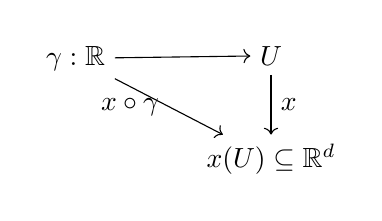
\begin{tikzpicture}[decoration=snake]
\matrix (m) [matrix of math nodes, row sep=2em, column sep=3em, minimum width=1em]
{
	\gamma : \mathbb{R} & U \\
	& x(U) \subseteq \mathbb{R}^d \\ 
};
\path[->]
(m-1-1) edge node [above] {$$} (m-1-2)
edge node [left] {$x\circ \gamma$} (m-2-2)
(m-1-2) edge node [right] {$x$} (m-2-2);
\end{tikzpicture}
\underline{idea}. try to ``lift'' the undergraduate notion of differentiability of a curve on $\mathbb{R}^d$ to a notion of differentiability of a curve on $M$

\underline{Problem} Can this be well-defined under change of chart?

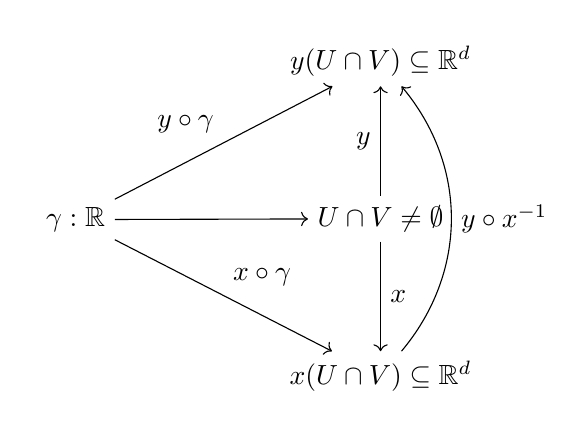
\begin{tikzpicture}[decoration=snake]
\matrix (m) [matrix of math nodes, row sep=4em, column sep=6em, minimum width=2em]
{
	& y(U\cap V) \subseteq \mathbb{R}^d \\ 
	\gamma : \mathbb{R} & U \cap V \neq \emptyset \\
	& x(U\cap V) \subseteq \mathbb{R}^d \\ 
};
\path[->]

(m-2-1) edge node [auto] {$$} (m-2-2)
edge node [auto] {$x\circ \gamma$} (m-3-2)
edge node [auto] {$y\circ \gamma$} (m-1-2)
(m-2-2) edge node [auto] {$x$} (m-3-2)
edge node [auto] {$y$} (m-1-2)
(m-3-2) edge [bend right=40] node [right] {$y\circ x^{-1}$} (m-1-2);
\end{tikzpicture}

$x\circ \gamma$ undergraduate differentiable (``as a map $\mathbb{R} \to \mathbb{R}^d$'')

\[
\begin{gathered}
\underbrace{y\circ \gamma}_{\text{maybe only continuous, but not undergraduate differentiable} } =  \underbrace{ ( \overbrace{ y\circ x^{-1}}^{\mathbb{R}^d \to \mathbb{R}^d }   )}_{\text{continuous}}  \circ \underbrace{ \overbrace{ (x\circ \gamma) }^{\mathbb{R}\to \mathbb{R}^d} }_{ \text{ undergrad differentiable } }  = y \circ (x^{-1} \circ x) \circ \gamma
\end{gathered}
\]

At first sight, strategy does not work out.  

\subsection{2. Compatible charts}

In section 1, we used any imaginable charts on the top. mfd. $(M,\mathcal{O})$.  

To emphasize this, we may say that we took $U$ and $V$ from the \emph{maximal atlas} $\mathcal{A}$ of $(M,\mathcal{O})$.  


\begin{definition}
Two charts $(U,x)$ and $(V,y)$ of a top. mfd. are called \ding{96}-compatible if 
either
\begin{enumerate}
\item[(a)] $U \cap V = \emptyset$
or  \item[(b)] $U\cap V \neq \emptyset$
\end{enumerate}
chart transition maps have undergraduate \ding{96} property.

EY : 20151109 e.g. since $\mathbb{R}^d \to \mathbb{R}^d$, can use undergradate \ding{96} property such as continuity or differentiability.

\[
\begin{aligned}
& y \circ x^{-1} : x(U \cap V) \subseteq \mathbb{R}^d  \to y(U\cap V) \subseteq \mathbb{R}^d  \\
& x\circ y^{-1} : y(U\cap V) \subseteq \mathbb{R}^d   \to x(U\cap V) \subseteq \mathbb{R}^d
\end{aligned}
\]
\end{definition}

\underline{Philosophy}: 

\begin{definition}
An atlas $\mathcal{A}_{\text{\ding{96}}}$ is a \ding{96}-compatible atlas if any two charts in $\mathcal{A}_{\text{\ding{96}}}$ are \ding{96}-compatible.

\end{definition}

\begin{definition}
A \textbf{\ding{96}-manifold} is a triple $(\underbrace{ M,\mathcal{O} }_{\text{top. mfd.} }, \mathcal{A}_{\text{\ding{96}}})$ \quad \, $\mathcal{A}_{\text{\ding{96}}} \subseteq \mathcal{A}_{\text{maximal}} $
\end{definition}


\begin{tabular}{ l | c  l}
\ding{96} &  undergraduate  \ding{96} &  \\
\hline
$C^0$ & $C^0(\mathbb{R}^d \to \mathbb{R}^d) =$  &  continuous maps w.r.t. $\mathcal{O}$  \\
$C^1$ & $C^1(\mathbb{R}^d \to \mathbb{R}^d) = $  &  differentiable (once) and is continuous  \\
$C^k$ & & $k$-times continuously differentiable \\
$D^k$ & & $k$-times differentiable \\
$\vdots$ & & \\
$C^{\infty}$ & $C^{\infty}(\mathbb{R}^d \to \mathbb{R}^d)$ & \\
$\mathbin{\rotatebox[origin=c]{-90}{$\supseteq$}}$ & &  \\
$C^{\omega}$ & $\exists $  multi-dim. Taylor exp.  &  \\
$\mathbb{C}^{\infty}$ & satisfy Cauchy-Riemann equations, pair-wise & 
\end{tabular}


EY : 20151109 Schuller says: $C^k$ is easy to work with because you can judge $k$-times cont. differentiability from existence of all partial derivatives \textbf{and} their continuity.  There are examples of maps that partial derivatives exist but are not $D^k$, $k$-times differentiable.  

\begin{theorem}[Whitney]
%  Any $C^{k\geq 1}$-manifold $(M,\mathcal{O}, \mathcal{A}_{C^{k\geq 1}})$  
Any $C^{k\geq 1}$-atlas, $\mathcal{A}_{C^{k\geq 1}}$ of a topological manifold \emph{contains} a $C^{\infty}$-atlas.  

Thus we may w.l.o.g. always consider $C^{\infty}$-manifolds, ``smooth manifolds'', unless we wish to define Taylor expandibility/complex differentiability \dots
\end{theorem}

EY : 20151109 Hassler Whitney \footnote{\url{http://mathoverflow.net/questions/8789/can-every-manifold-be-given-an-analytic-structure}}

\begin{definition}
A smooth manifold $(\underbrace{ M,\mathcal{O} }_{\text{top. mfd. } }, \underbrace{ \mathcal{A}}_{C^{\infty}-\text{atlas}} )$ 
\end{definition}

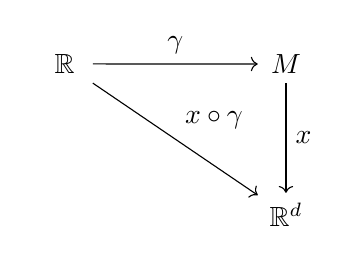
\begin{tikzpicture}
\matrix (m) [matrix of math nodes, row sep=4em, column sep=6em, minimum width=2em]
{
	\mathbb{R} & M   \\
	&  \mathbb{R}^d \\ 
};
\path[->]  
(m-1-1) edge node [auto] {$\gamma$} (m-1-2)
edge node [auto] {$x\circ \gamma$} (m-2-2)
(m-1-2) edge node [auto] {$x$} (m-2-2);
\end{tikzpicture}
EY: 20151109 Schuller was explaining that the trajectory is real in $M$; the coordinate maps to obtain coordinates is $x\circ \gamma$

\subsection{4. Diffeomorphisms}

$M \xrightarrow{ \phi } N$

If $M,N$ are naked sets, the structure preserving maps are the bijections (invertible maps).  

e.g. $\lbrace 1,2,3 \rbrace \to \lbrace a,b \rbrace$

\begin{definition}
	$M \cong_{\text{set}} N$ (set-theoretically) isomorphic if $\exists \, $ bijection $\phi : M \to N$
\end{definition}

\underline{Examples}.  $\mathbb{N} \cong_{\text{set}} \mathbb{Z}$ \\
$\mathbb{N} \cong_{\text{set}} \mathbb{Q}$  (EY: 20151109 Schuller says from diagonal counting)\\
$\mathbb{N} \cancel{\cong_{\text{set}}} \mathbb{R}$

Now $(M, \mathcal{O}_M) \cong_{\text{top}} (N,\mathcal{O}_N)$ (topl.) isomorphic $=$ ``homeomorphic'' $\exists \, $ bijection $\phi : M \to N$  \\
\phantom{ \quad \quad \, } $\phi, \phi^{-1}$ are continuous.  

$(V,+,\cdot) \cong_{\text{vec}} ( W,+_w,\cdot_w)$ (EY: 20151109 vector space isomorphism) if \\
$\exists \, \text{ bijection } \phi : V \to W$ linearly

\underline{finally}

\begin{definition}
	Two $C^{\infty}$-manifolds \\
	$(M,\mathcal{O}_M, \mathcal{A}_M)$ and $(N,\mathcal{O}_N, \mathcal{A}_N)$ are said to be \textbf{diffeomorphic} if $\exists \, $ bijection $\phi : M \to N$ s.t. 
	\[
	\begin{aligned} & \phi : M \to N \\
	& \phi^{-1} : N \to M \end{aligned}
	\]
	are both $C^{\infty}$-maps
	
	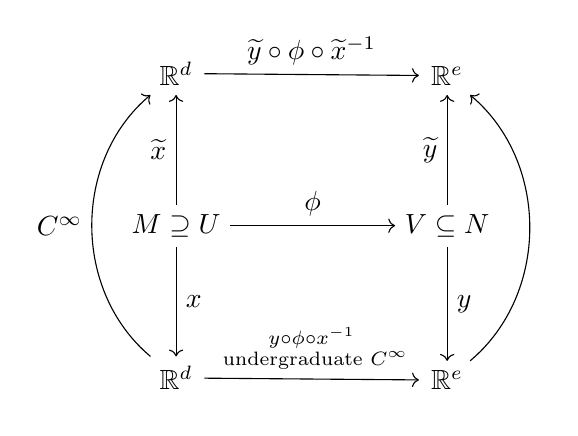
\begin{tikzpicture}
	\matrix (m) [matrix of math nodes, row sep=4em, column sep=6em, minimum width=2em]
	{
		\mathbb{R}^d & \mathbb{R}^e   \\
		M \supseteq U &  V\subseteq N   \\ 
		\mathbb{R}^d & \mathbb{R}^e \\
	};
	\path[->]  
	(m-1-1) edge node [auto] {$\widetilde{y} \circ \phi \circ \widetilde{x}^{-1}$} (m-1-2)
	(m-2-1) edge node [auto] {$\widetilde{x}$} (m-1-1)
	edge node [auto] {$\phi$} (m-2-2)
	edge node [auto] {$x$} (m-3-1)
	(m-3-1) edge node [auto] {$ \substack{ y\circ \phi \circ x^{-1} \\ 
			\text{ undergraduate } C^{\infty} }$} (m-3-2)
	edge [bend left=50] node [auto] {$C^{\infty}$} (m-1-1)
	(m-2-2) edge node [auto] {$\widetilde{y}$} (m-1-2) 
	edge node [auto] {$y$} (m-3-2)
	(m-3-2) edge [bend right=50] node [auto] {$$} (m-1-2);
	\end{tikzpicture}
	
	
	\end{definition}
	
	\begin{theorem}
	$\# = $ number of $C^{\infty}$-manifolds one can make out of a given $C^0$-manifolds (if any) - up to diffeomorphisms.  
	
	\begin{tabular}{l | c r }
	$\text{dim}M$ &  $\#$ &  \\
	\hline
	1  & 1  & Morse-Radon theorems \\
	2  & 1  & Morse-Radon theorems \\
	3 & 1  & Morse-Radon theorems \\
	4 & uncountably infinitely many & \\
	5 &   finite  & surgery theory \\
	6 &  finite & surgery theory \\
	\vdots & finite & surgery theory
	\end{tabular}
	
	\end{theorem}
	
	EY : 20151109 cf. \url{http://math.stackexchange.com/questions/833766/closed-4-manifolds-with-uncountably-many-differentiable-structures}  \\
	\href{http://www.maths.ed.ac.uk/~aar/papers/scorpan.pdf}{The wild world of 4-manifolds}
	
	
	\section*{Tutorial 4 Differentiable Manifolds}
	
	EY : 20151109 The \url{gravity-and-light.org} website, where you can download the tutorial sheets \emph{and} the full length videos for the tutorials and lectures, are no longer there.  $=($  
	
	Hopefully, the YouTube video will remain: \url{https://youtu.be/FXPdKxOq1KA?list=PLFeEvEPtX_0RQ1ys-7VIsKlBWz7RX-FaL}
	
	\exercisehead{1: True or false?} \emph{These basic questions are designed to spark discussion and as a self-test.}
	
	Tick the correct statements, but not the incorrect ones!
	
	\begin{enumerate}
	\item[(a)] The function $f: \mathbb{R} \to \mathbb{R}$, \dots
	\begin{itemize}
	\item  
	\item
	\item \dots , defined by $f(x) = |x^3|$, lies in $C^3(\mathbb{R} \to \mathbb{R})$.  
	
	EY : 20151109 \solutionhead{1a3} For $f: \mathbb{R} \to \mathbb{R}$, $f(x) = |x^3| = \begin{cases} x^3 & \text{ if } x \geq 0 \\
	-x^3 & \text{ if } x < 0 \end{cases}$ 
	\[
	\begin{aligned}
	& f'(x) = \begin{cases} 3x^2  & \text{ if } x \geq 0 \\
	-3x^2 & \text{ if } x < 0 \end{cases} \\ 
	& f''(x) = \begin{cases} 6x  & \text{ if } x \geq 0 \\
	-6x & \text{ if } x < 0 \end{cases} 
	\end{aligned}
	\]
	Thus, 
	\[
	\boxed{ f(x) = |x^3| \in C^1(\mathbb{R}) \text{ but } f(x) \notin C^2(\mathbb{R}) \subseteq C^3(\mathbb{R}) }
	\]
	\item
	\item
	\end{itemize}
	\item[(b)]
	\item[(c)]
	\end{enumerate}
	
	\textbf{Short} \exercisehead{4: Undergraduate multi-dimensional analysis }
	
	\emph{A good notation and basic results for partial differentiation}.
	
	For a map $f: \mathbb{R}^d \to \mathbb{R}$ we denote by the map $\partial_i f: \mathbb{R}^d \to \mathbb{R}$ the partial derivative with respect to the $i$-th entry.
	
	\questionhead{:} Given a function
	\[
	f: \mathbb{R}^3 \to \mathbb{R}; \, (\alpha, \beta, \delta) \mapsto f(\alpha,\beta,\delta) := \alpha^3\beta^2 + \beta^2 \delta + \delta
	\]
	calculate the values of the following derivatives:
	
	\solutionhead{:}
	
	\begin{itemize}
	\item $(\partial_2f)(x,y,z) = $
	\item $(\partial_1f)(\square,\circ,*) =$
	\item $(\partial_1 \partial_2 f)(a,b,c) = $ 
	\item $(\partial_3^2 f)(299,1222,0) =$
	\end{itemize}
	
	EY: 20151110
	
	For $f(\alpha,\beta,\delta) := \alpha^3\beta^2 + \beta^2 \delta + \delta$, or $f(x,y,z) = x^3 y^2 + y^2 z + z$, 
	\[
	\begin{aligned}
	& (\partial_2 f) = 2(x^3y+yz) \\ 
	& (\partial_1 f) = 3x^2 y^2 \\ 
	& (\partial_1\partial_2 f) = 6x^2 y \\ 
	& (\partial_3^2f) = 0 
	\end{aligned}
	\]
	and so 
	\begin{itemize}
	\item $(\partial_2f)(x,y,z) = 2(x^3 y + yz)  $
	\item $(\partial_1f)(\square,\circ,*) = 3\square^2 \circ^2$
	\item $(\partial_1 \partial_2 f)(a,b,c) = 6a^2 b$ 
	\item $(\partial_3^2 f)(299,1222,0) = 0$
	\end{itemize}
	
	
	
	\exercisehead{5: Differentiability on a manifold}
	
	\emph{How to deal with functions and curves in a chart} 
	
	Let $(M, \mathcal{O}, \mathcal{A})$ be a smooth $d$-dimensional manifold.  Consider a chart $(U,x)$ of the atlas $\mathcal{A}$ together with a smooth curve $\gamma : \mathbb{R} \to U$ and a smooth function $f:U \to \mathbb{R}$ on the domain $U$ of the chart. 
	
	\questionhead{:} Draw a commutative diagram containing the chart domain, chart map, function, curveand the respective representatives of the function and the curve in the chart. 
	
	\solutionhead{:}
	
	\begin{tikzpicture}[decoration=snake]
	\matrix (m) [matrix of math nodes, row sep=4em, column sep=6em, minimum width=2em]
	{
		\mathbb{R} & U & \mathbb{R}^d \\
		& \mathbb{R} &  \\
	};
	\path[->]
	(m-1-1) edge node [above] {$\gamma$} (m-1-2)
	edge [bend left=40] node [auto] {$x\circ \gamma$} (m-1-3)
	(m-1-3) edge [bend left=15] node [auto] {$x^{-1}$} (m-1-2)
	edge node [right] {$(f\circ x^{-1})$ } (m-2-2)
	(m-1-2) edge node [left] {$f$} (m-2-2)
	edge node [auto] {$x$} (m-1-3);
	\end{tikzpicture} \quad \quad \, \begin{tikzpicture}[decoration=snake]
	\matrix (m) [matrix of math nodes, row sep=4em, column sep=6em, minimum width=2em]
	{
		\tau \in \mathbb{R} & p \in U & x(p) = (x\circ \gamma)(\tau) \in \mathbb{R}^d \\
		& f(p) \in \mathbb{R} &  \\
	};
	\path[|->]
	(m-1-1) edge node [above] {$\gamma$} (m-1-2)
	edge [bend left=40] node [auto] {$x\circ \gamma$} (m-1-3)
	(m-1-3) edge [bend left=15] node [auto] {$x^{-1}$} (m-1-2)
	edge node [right] {$(f\circ x^{-1})$ } (m-2-2)
	(m-1-2) edge node [left] {$f$} (m-2-2)
	edge node [auto] {$x$} (m-1-3);
	\end{tikzpicture}
	
	
	
	\questionhead{:} Consider, for $d=2$,
	\[
	(x\circ \gamma)(\lambda):= (\cos{(\lambda)}, \sin{(\lambda)} ) \text{ and } (f\circ x^{-1})((x,y)) := x^2 +y^2
	\]
	Using the chain rule, calculate
	\[
	(f\circ \gamma)'(\lambda)
	\]
	explicitly.
	
	\solutionhead{:}
	
	EY : 20151109 Indeed, the domains and codomains of this $f\gamma$ mapping makes sense, from $\mathbb{R} \to \mathbb{R}$ for 
	\begin{tikzpicture}[decoration=snake]
	\matrix (m) [matrix of math nodes, row sep=4em, column sep=6em, minimum width=2em]
	{
		\mathbb{R} & U & \mathbb{R}^d \\
		& \mathbb{R} &  \\
	};
	\path[->]
	(m-1-1) edge node [above] {$\gamma$} (m-1-2)
	edge [bend left=40] node [auto] {$x\circ \gamma$} (m-1-3)
	edge node [auto] {$f\circ \gamma$} (m-2-2)
	(m-1-3) edge [bend left=15] node [auto] {$x^{-1}$} (m-1-2)
	edge node [right] {$(f\circ x^{-1})$ } (m-2-2)
	(m-1-2) edge node [left] {$f$} (m-2-2)
	edge node [auto] {$x$} (m-1-3);
	\end{tikzpicture} \quad \quad \, \begin{tikzpicture}[decoration=snake]
	\matrix (m) [matrix of math nodes, row sep=4em, column sep=6em, minimum width=2em]
	{
		\tau \in \mathbb{R} & p \in U & x(p) = (x\circ \gamma)(\tau) \in \mathbb{R}^d \\
		& f(p) \in \mathbb{R} &  \\
	};
	\path[|->]
	(m-1-1) edge node [above] {$\gamma$} (m-1-2)
	edge [bend left=40] node [auto] {$x\circ \gamma$} (m-1-3)
	edge node [auto] {$f\circ \gamma$} (m-2-2)
	(m-1-3) edge [bend left=15] node [auto] {$x^{-1}$} (m-1-2)
	edge node [right] {$(f\circ x^{-1})$ } (m-2-2)
	(m-1-2) edge node [left] {$f$} (m-2-2)
	edge node [auto] {$x$} (m-1-3);
	\end{tikzpicture}
	
	\[
	\begin{gathered}
	(f\circ \gamma)'(\lambda) = (Df)\cdot \dot{\gamma}(\lambda) = \frac{ \partial f}{ \partial x^j} \dot{\gamma}^j(\lambda) = 2x (-\sin{\lambda} ) + 2y \cos{\lambda} = 2(-\cos{\lambda} \sin{\lambda} + \sin{\lambda} \cos{\lambda} ) = 0 
	\end{gathered}
	\]
	
	
	
	\section{Lecture 5: Tangent Spaces}
	
	lead question: ``what is the velocity of a curve $\gamma$ \@ point $p$?
	
	\subsection{Velocities}
	
	\begin{definition}
		$(M,\mathcal{O},\mathcal{A})$ smooth mfd. \\
		curve $\gamma : \mathbb{R} \to M$ at least $C^1$.   \\
		Suppose $\gamma(\lambda_0) =p$ \\
		The \textbf{velocity} of $\gamma$ \@ $p$ is the linear map 
		\[
		\begin{gathered}
		v_{\gamma, p} : C^{\infty}(M) \xrightarrow{ \sim } \mathbb{R}
		\end{gathered}
		\]
		$C^{\infty}(M) := \lbrace f: M \to \mathbb{R} | f \text{ smooth function } \rbrace$ equipped with $\begin{gathered}  \quad \\ 
		(f\oplus g)(p) := f(p) + g(p) \\
		(\lambda \otimes g)(p) := \lambda \cdot g(p) \end{gathered}$
		
		$\sim$ denotes linear map on top of $\xrightarrow{}$.
		
		\[
		f \mapsto v_{\gamma,p}(f):= (f\circ \gamma)'(\lambda_0)
		\]
		
		
	\end{definition}
	
	intuition
	\begin{tikzpicture}
	\matrix (m) [matrix of math nodes, row sep=4em, column sep=6em, minimum width=2em]
	{
		\mathbb{R} & M  & \mathbb{R}   \\
	};
	\path[->]  
	(m-1-1) edge node [auto] {$\gamma$} (m-1-2)
	edge [bend right=40] node [auto] {$f\circ \gamma $} (m-1-3)
	(m-1-2) edge node [auto] {$f $} (m-1-3);
	\end{tikzpicture}
	
	
	
	Schuller says: children run around the world.  Temperature function as temperature contour lines.  You feel the temperature.  You observe the rate of change of temperature as you run around.  $f$ is temperature.  
	
	\underline{past}: `` $\underbrace{v^i}_{} (\partial_i f) = (\underbrace{v^i \partial_i}_{\text{vector}})f$ 
	
	\subsection{Tangent vector space}
	
	\begin{definition}
		For each point $p \in M$ \\
		def the \textbf{set} ``tangent space $\neq_0 M$ \@ $p$ ``
		\[
		T_p M := \lbrace v_{\gamma, p} | \gamma \text{ smooth curves } \rbrace
		\]
	\end{definition}
	
	\underline{picture}:\\
	rather $M$ than (embedded) $p$ $T_pM$ EY : 20151109 see \url{https://youtu.be/pepU_7NJSGM?t=12m38s} for the picture
	
	\underline{Observation}: $T_pM$ can be made into a vector space. 
	
	\[
	\begin{aligned}
	& \begin{aligned}
	\oplus : & T_pM \times T_pM \to   \\
	& (v_{\gamma,p} \oplus v_{\delta,p})(\underbrace{f}_{ \in C^{\infty}(M)} ) := v_{\gamma,p}(f) +_{\mathbb{R}} v_{\delta,p}(f) \\
	\end{aligned} \\
	& \begin{aligned}
	\odot : & \mathbb{R} \times T_pM \to \text{Hom}(C^{\infty}(\mathbb{R}),\mathbb{R}) \\
	& (\alpha \odot v_{\gamma,p} )(f) := \alpha \cdot_{\mathbb{R}}  v_{\gamma, p}(f)
	\end{aligned}
	\end{aligned}
	\]
	Remains to be shown that 
	\begin{enumerate}
		\item[(i)] $\exists \, \sigma$ curve : $v_{\gamma,p} \oplus v_{\delta,p} = v_{\sigma,p}$
		\item[(ii)] $\exists \, \tau $ curve : $\alpha \odot v_{\gamma,p} = v_{\tau,p}$
	\end{enumerate}
	
	\underline{Claim}: $\begin{aligned} & \quad \\ 
	\tau : \mathbb{R}&  \to M  \\
	& \mapsto \tau(\lambda) := \gamma(\alpha  \lambda + \lambda_0) = (\gamma \circ \mu_{\alpha})(\lambda)
	\end{aligned}$
	where $\begin{aligned} & \quad \\
	\mu_{\alpha}: & \mathbb{R} \to \mathbb{R} \\ 
	& r \mapsto \alpha \cdot r + \lambda_0 \end{aligned}$, 
	does the trick.
	
	$\tau(0) = \gamma(\lambda_0) =p$
	
	\[
	\begin{aligned}
	v_{\tau,p} & := (f\circ \tau)'(0) = (f\circ \gamma \circ \mu_{\alpha} )'(0) \\ 
	& =  (f\circ \gamma)'(\lambda_0) \cdot \alpha = \\
	& = \alpha \cdot v_{\gamma,p}
	\end{aligned}
	\]
	
	Now for the sum: %(EY:20151109 ??)
	
	$v_{\gamma,p} \oplus v_{\delta,p} \overset{?}{=} v_{\sigma, p} $
	
	make a \underline{choice} of chart $(\underbrace{U}_{\ni p} , x)$  In cloud: ill definition alarm bells. 
	
	and define:
	
	Claim:
	\[
	\begin{aligned}
	& \sigma : \mathbb{R} \to M \\
	& \sigma(\lambda) := x^{-1}( \underbrace{ (x\circ \gamma)(\lambda_0 + \lambda)}_{\mathbb{R} \to \mathbb{R}^d}  + (x\circ \delta)(\lambda_1+ \lambda) - (x\circ \gamma)(\lambda_0) )
	\end{aligned}
	\]
	does the trick.
	\begin{proof}
		Since: 
		\[
		\begin{aligned}
		\sigma_x(0) & = x^{-1}((x\circ \gamma)(\lambda_0) + (x\circ \delta)(\lambda_1) - (x\circ \gamma)(\lambda_0)) \\
		& = \delta(\lambda_1) = p \end{aligned}
		\]
		Now:
		\[
		\begin{aligned}
		v_{\sigma_x,p}(f) & := (f\circ \sigma_x)'(0) =  \\ 
		& = ( \underbrace{ (f\circ x^{-1}) }_{\mathbb{R}^d \to \mathbb{R}}  \circ \underbrace{ (x\circ \sigma_x) }_{\mathbb{R} \to \mathbb{R}^d}  )'(\gamma) = \underbrace{ (x\circ \sigma_x)'(0) }_{(x\circ \gamma)'(\lambda_0) + (x\circ \delta)'(\lambda_1) } \cdot \left( \partial_i (f\circ x^{-1}) \right)(x( \underbrace{ \sigma(0)}_{p} ) ) = \\
		& = (x\circ \gamma)'(\lambda_0)(\partial_i (f\circ x^{-1}) )(x(p)) + (x\circ \delta)(\lambda_1)(\partial_i (f\circ x^{-1})  )(x(p)) \\
		& = (f\circ \gamma)'(\lambda_0) + (f\circ \delta)'(\lambda_1) = \\
		& = v_{\gamma,p}(f) + v_{\delta,p}(f) \quad \, \forall \, f \in C^{\infty}(M)
		\end{aligned}
		\]
		
		\[
		\boxed{ v_{\gamma,p} \oplus v_{\delta,p} = v_{\sigma, p} }
		\]
	\end{proof}
	
	\begin{tikzpicture}
	\matrix (m) [matrix of math nodes, row sep=4em, column sep=6em, minimum width=2em]
	{
		\mathbb{R} & M  & \mathbb{R}   \\
		& \mathbb{R}^d & \\ 
	};
	\path[->]  
	(m-1-1) edge node [auto] {$\sigma$} (m-1-2)
	edge  node [auto] {$x\circ \sigma $} (m-2-2)
	(m-1-2) edge node [auto] {$x $} (m-2-2)
	edge node [auto] {$f$} (m-1-3)
	(m-2-2) edge node [below] {$f\circ x^{-1}$} (m-1-3);
	\end{tikzpicture}
	
	
	\underline{picture}: (cf. \url{https://youtu.be/pepU_7NJSGM?t=39m5s})
	
	\[
	\begin{aligned} 
	\gamma : \mathbb{R} \to M \\
	\delta : \mathbb{R} \to M \end{aligned}
	\]
	$(\gamma \oplus)(\lambda) := \gamma(\lambda) + \delta(\lambda)$
	
	EY : 20151109 Schuller says adding trajectories is chart dependent, bad. Adding velocities is good.  
	\subsection{Components of a vector wrt a chart}
	
	\begin{definition}
		Let $(U,x) \in \mathcal{A}_{\text{smooth}}$.  \\
		Let $\begin{aligned} & \gamma : \mathbb{R} \to U \\ 
		& \gamma(0) = p \end{aligned}$.  
		
		Calculate 
		\[
		\begin{aligned} 
		v_{\gamma,p}(f) & := (f \circ \gamma)'(0) = (\underbrace{ (f\circ x^{-1}) }_{\mathbb{R}^d \to \mathbb{R} }  \circ \underbrace{ (x\circ \gamma)}_{\mathbb{R} \to \mathbb{R}^d}  )'(0) \\
		& = \underbrace{ (x\circ \gamma)^{i'}(0) }_{\dot{\gamma}_x^i(0) }  \cdot \underbrace{ (\partial_i(f\circ x^{-1} ) )(x(p))  }_{ =: \left( \frac{ \partial f}{ \partial x^i } \right)_p }
		\end{aligned}
		\]
		think cloud $f:M\to \mathbb{R}$
		\[
		= \boxed{ \dot{\gamma}_x^i(0) \cdot \left( \frac{ \partial }{ \partial x^i} \right)_p } f \quad \, \forall \, f \in C^{\infty}(M)
		\]
		$\therefore$ as a map.  
		
		\[
		v_{\gamma,p} \underbrace{=}_{\text{use of chart} } \underbrace{ \gamma_x^i(0) }_{ \text{ ``components of the velocity $v_{\gamma,p}$'' } } \underbrace{ \left( \frac{ \partial }{ \partial x^i} \right)}_{ \substack{ \text{ basis elements of the $T_pM$ wrt which the components need to be understood.} \\
				\text{ ``chart induced basis of $T_pM$''} } } 
		\]
	\end{definition}
	
	Picture: \url{https://youtu.be/pepU_7NJSGM?t=1h16s}
	
	\subsection{4. Chart-induced basis}
	
	\begin{definition}
		$(U,x) \in \mathcal{A}_{\text{smooth}}$ \\
		the $\left( \frac{ \partial }{ \partial x^1} \right)_p , \dots , \left( \frac{ \partial }{ \partial x^d} \right)_p \in T_pU \subseteq T_pM$
		
		constitute a \textbf{basis} of $T_pU$
		
	\end{definition}
	
	\begin{proof} remains: linearly independent 
		\[
		\begin{gathered}
		\lambda^i \left( \frac{ \partial }{ \partial x^i} \right)_p \overset{!}{=} 0  \\
		\Longrightarrow \lambda^i \left( \frac{ \partial }{ \partial x^i} \right)_p(x^j) = \lambda^i \partial_i (\underbrace{ x^j \circ x^{-1} }_{} )( x(p)) = \\
		= \lambda^i \delta_i^{\,\,j} = \lambda^j \quad \quad \, j = 1 , \dots , d
		\end{gathered} \quad \quad \, \begin{gathered}
		x^j \circ x^{-1} : \mathbb{R}^d \to \mathbb{R} \\
		(\alpha^1 , \dots , \alpha^d) \mapsto \alpha^j 
		\end{gathered}
		\]
		in cloud: $x^j : U \to \mathbb{R}$ differentiable
		
		
		
		
	\end{proof}
	
	
	\begin{corollary}
		$ \text{dim}T_pM = d = \text{dim}M$
	\end{corollary}
	
	\underline{Terminology}: $X \in T_pM$ $\to $ $\exists \, \gamma : \mathbb{R} \to M : X = v_{\gamma,p}$ and \\
	\phantom{\underline{Terminology}:} $\exists \, \underbrace{ X_1^1 , \dots , X^d }_{\in \mathbb{R} } : X = X^i \left( \frac{ \partial }{ \partial x^i} \right)_p$
	
	
	
	\subsection{5. Change of vector \emph{\underline{components}} under a change of chart}
	
	\ding{56} vector does \textbf{not} change under change of chart.
	
	Let $(U,x)$ and $(V,y)$ be overlapping charts and $p \in U\cap V$.  \\
	Let $X \in T_pM$
	
	\[
	X^i_{(y)}\cdot \left( \frac{ \partial }{ \partial y^i} \right)_p \underbrace{=}_{(V,y)} X \underbrace{=}_{ (U,x) } X^i_{x} \left( \frac{ \partial }{ \partial x^i} \right)_p
	\]
	to study change of components formula:
	\[
	\begin{aligned}
	\left( \frac{ \partial }{ \partial x^i} \right)_p f & = \partial_i(f\circ x^{-1} )(x(p)) =  \\
	& = \partial_i (\underbrace{ (f\circ y^{-1}) }_{\mathbb{R}^d \to \mathbb{R} } \circ (\underbrace{ y\circ x^{-1}}_{\mathbb{R}^d \to \mathbb{R}^d} )(x(p)) \\
	& = (\partial_i (y^i\circ x^{-1} ) )(x(p)) \cdot (\partial_j (f\circ y^{-1}) )(y(p)) = \\
	& = \boxed{ \left( \frac{ \partial y^p}{ \partial x^i} \right)_p \cdot \left( \frac{ \partial f}{ \partial y^j} \right)_p  } f
	\end{aligned}
	\]
	\[
	\begin{gathered}
	\Longrightarrow X^i_{(x)} \left( \frac{ \partial y^j}{ \partial x^i} \right)_p \left( \frac{ \partial }{ \partial y^j} \right)_p = X^j_{(y)}\left( \frac{ \partial }{ \partial y^j} \right)_p \\
	\Longrightarrow \boxed{ X^j_{(y)} = \left( \frac{ \partial y^j}{ \partial x^i} \right)_pX^i_{(x)} }
	\end{gathered}
	\]
	
	\subsection{6. Cotangent spaces }
	
	$T_pM = V$
	
	trivial $(T_pM)^* := \lbrace \varphi : T_pM \xrightarrow{\sim} \mathbb{R} \rbrace$
	
	\underline{Example}: $f\in C^{\infty}(M)$ 
	
	\[
	\begin{aligned}
	(df)_p : & T_p M \xrightarrow{ \sim } \mathbb{R} \\ 
	& X \mapsto (df)_p(X)
	\end{aligned}
	\]
	i.e. $\boxed{ (df)_p \in T_pM^* } $
	
	$(df)_p$ called the gradient of $f$ \@ $p\in M$.  
	
	Calculate components of gradient w.r.t. chart-induced basis $(U,x)$  
	
	\[
	\begin{aligned}
	\left( (df)_p \right)_j & := (df)_p\left( \left( \frac{ \partial }{ \partial x^j} \right)_p \right) \\
	& = \left( \frac{ \partial f}{ \partial x^j } \right)_p = \partial_j (f\circ x^{-1} )(x(p))
	\end{aligned}
	\]
	
	\begin{theorem}
		Consider chart $(U,x)  \Longrightarrow x^i : U \to \mathbb{R}$  
		
		\underline{Claim}: $(d x^1)_p, (dx^2)_p, \dots , (dx^d)_p$ basis of $T_p^*M$ 
		
		$\Longrightarrow $ In fact: dual basis: 
		\[
		(dx^a)_p \left( \left( \frac{ \partial }{ \partial x^b} \right)_p \right) = \left( \frac{ \partial x^a}{ \partial x^b} \right)_p = \dots = \delta_b^a
		\]
	\end{theorem}
	
	\subsection{ 7. Change of \emph{ \underline{components} } of a covector under a change of chart: }
	
	\[
	\begin{gathered}
	\underbrace{ T_p^*M }_{ \ni \omega} \text{ with } 
	\omega_{(y)} (dy^j)_p =   \omega = \omega_{(x)i} (dx^i)_p  \\
	\Longrightarrow \boxed{ \omega_{(y)i} = \frac{ \partial x^j}{ \partial y^i } \omega_{(x)j } }
	\end{gathered}
	\]
	
	
	
	
	
	
	
	
	\section*{Lecture 6: Fields}
	
cf. \href{https://youtu.be/UbQS40KHkH0}{Lecture 6: Fields (International Winter School on Gravity and Light 2015)}
	
	So far: 
	
	\begin{tikzpicture}[decoration=snake]
	\matrix (m) [matrix of math nodes, row sep=2em, column sep=3em, minimum width=1em]
	{
		T_pM \\ 
		T_p^*M \\
		\vdots \\
	};
	\path[->] %,decorate={zigzag,amplitude=0.7pt, segment length=1.2mm, pre=lineto,pre length=4pt}]
	(m-1-1) edge node [left] {$\vdots$} (m-2-1)
	(m-2-1) edge node [left] {$\vdots$} (m-3-1);
	\end{tikzpicture},
	
	now
	
	in Thought Cloud: theory of bundles
	
	\subsection{Bundles}
	
	\begin{definition}
		A \textbf{bundle} is a triple 
		\[
		E \xrightarrow{ \pi } M 
		\]
		$E$ smooth manifold \quad \, ``\textbf{total space}'' \\
		$\pi$ smooth map (surjective)  ``projection map'' \\
		$M$ smooth manifold ``base space''
		
	\end{definition}
	
	\underline{Example} $E = $ cylinder
	$M = $ circle
	
	
	\begin{definition}
\[
\begin{tikzcd}
E \arrow[r, "T"] & M \\
\end{tikzcd}
\] bundle.



$p \in M$

		\emph{define} \textbf{fibre over $p$} \\
		\phantom{define} $:= \text{preim}_{\pi}(\lbrace p \rbrace)$
	\end{definition}
	
	\begin{definition}
		A \textbf{section} $\sigma$ of a bundle
		
		\begin{tikzpicture}
		\matrix (m) [matrix of math nodes, row sep=2em, column sep=3em, minimum width=1em]
		{
			E \\
			M \\ };
		\path[->]
		(m-1-1) edge node [left] {$\pi$} (m-2-1)
		(m-2-1) edge [bend right=45] node [right] {$\sigma$} (m-1-1);
		\end{tikzpicture}
		
		
		
		
		
		require $\pi \circ \sigma = \text{id}_M$
	\end{definition}
	
	Schuller says: in quantum mechanics, 
	\underline{Aside}: $\psi : M \to \mathbb{C}$
	
	
	\subsection{Tangent bundle of smooth manifold}
	
	$(M,\mathcal{O},\mathcal{A})$ smooth manifold
	
	\begin{enumerate}
		\item[(a)] as a \textbf{set}
		$TM : = \dot{\bigcup}_{p\in M} T_pM$
		\item[(b)] $\begin{aligned} & \quad \\
		\text{surjective } & \pi: TM \to M \\
		& X\mapsto p \end{aligned}$ the \emph{unique} point $p\in M$, $X \in T_pM$  
		
		\underline{situation}:  $\underbrace{TM}_{\text{set}} \underbrace{ \xrightarrow{ \pi } }_{\text{surjective map }} \underbrace{M}_{\text{smooth manifold}}$
		
		\item[(c)] Construct topology on $TM$ that is the coarsest topology such that $\pi$ (just) continuous.  (``initial topology with respect to $\pi$'').
		
		\[
		\mathcal{O}_{TM} := \lbrace \text{preim}_{\pi}(U) | \mathcal{U}\in \mathcal{O} \rbrace
		\]
		Show: Tutorial $\mathcal{O}_{TM}$
		Schuller says this is shown in the tutorial
		
		$(TM,\mathcal{O}_{TM})$  \\
		
		\underline{Construction of a $C^{\infty}$-atlas on $TM$ from the $C^{\infty}$-atlas $\mathcal{A}$ on $M$. }
		
		\[
		\mathcal{A}_{TM} := \lbrace (T\mathcal{U},\xi_x  ) | (U,x) \in \mathcal{A} \rbrace
		\]
		where
		\[
		\begin{aligned}
		\xi_x : & T \mathcal{U} \to \mathbb{R}^{2\cdot\text{dim}  M } \\
		& X \mapsto (\underbrace{ (x^1 \circ \pi)(X), \dots, (x^d\circ \pi)(X) }_{(U,x)-\text{ coords of $\pi(X)$ } \, (d \text{ many } ) } , (dx^1)_{\pi(X)}(X), \dots , (dx^d)_{\pi(X)}(X)  )
		\end{aligned}
		\]
		where $X\in T_{\pi(X)}M$ \\
		\phantom{where } $X = X_{(x)}^i \left( \frac{ \partial }{ \partial x^i} \right)_{\pi(X)}$  \\
		\phantom{where } $\begin{aligned} \quad  & \\
		(dx^j)_{\pi(X)}(X) &= (dx^j)_{\pi(X)} \left( X^i_{(x)}\left( \frac{ \partial }{ \partial x^i} \right)_{\pi(X)} \right) = \\
		& = X^i_{(x)}\delta_i^j = X^j_{(x)}\end{aligned}$
		
		\underline{Write} $\xi_x^{-1} : \xi_x(TU) \subseteq \mathbb{R}^{2\text{dim}M} \to TU$
		\[
		(\alpha^1 , \dots , \alpha^d, \beta^1, \dots , \beta^d) := \beta^i \left( \frac{ \partial }{ \partial x^i} \right)_{ \underbrace{ x^{-1}(\alpha^1 , \dots , \alpha^d) }_{\pi(X)} }
		\]
		
		\underline{Check}: \[
		\begin{gathered}
		(\xi_y \circ \xi_x^{-1})(\alpha^1 , \dots , \alpha^d, \beta^1, \dots , \beta^d) = \\
		= \xi_y \left( \beta^i \left( \frac{ \partial }{ \partial x^i} \right)_{x^{-1}(\alpha^1 , \dots , \alpha^d) } \right) \\
		= \left( \dots, (y^i \circ \pi)( \beta^m \cdot \left( \frac{ \partial }{ \partial x^m} \right)_{x^{-1}(\alpha^1 \dots \alpha^d) } )  , \dots , \dots (dy^i)_{x^{-1}(\alpha^1, \dots \alpha^d) } \left( \beta^m \left( \frac{ \partial }{ \partial x^m} \right)_{x^{-1}(\alpha^1 \dots \alpha^d) } \right) , \dots   \right) = \\
		= ( \dots , (y^i \circ x^{-1})(\alpha^1 , \dots , \alpha^d), \dots , \dots , \underbrace{ \beta^m(dy^i)_{x^{-1} (\alpha^1, \dots , \alpha^d) } \left( \left( \frac{ \partial }{ \partial x^m} \right)_{x^{-1}(\alpha^1 \dots \alpha^d) } \right)}_{ \beta^m \left( \frac{ \partial y }{ \partial x^m } \right)_{x^{-1}(\alpha^1 \dots \alpha^d)} }  ) 
		\end{gathered}
		\]
		
		Check transition map: $(U, x), (V,y)$, \, $U\cap V \neq 0$
		
		%
		$\left( \frac{ \partial y }{ \partial x^m } \right)_{x^{-1}(\alpha^1 \dots \alpha^d)} = \partial_m (y^i \circ x^{-1} )( x\circ (x^{-1}(\alpha^1 \dots \alpha^d) ) ) = \partial_m (y^i \circ x^{-1} )( \alpha^1 \dots \alpha^d)$ smooth.  
		
		\underline{upshot}
		
		\[
		\underbrace{TM}_{\text{smooth manifold}} \underbrace{ \xrightarrow{\pi} }_{\text{smooth map} } \underbrace{M}_{\text{ smooth manifold} }
		\]
		bundle, called the tangent bundle.
		
	\end{enumerate}
	
	\subsection*{3. Vector fields}
	
	\begin{definition}
		A \textbf{smooth vector field} $\chi$ is a \emph{smooth} map, (where)
		\[
\begin{tikzcd}
TM \arrow[d, swap, "\pi"] \\
M \arrow[bend right=60,swap]{u}{\chi} \\
\end{tikzcd}		
	\]
	\end{definition}

Example:

\[
\begin{tikzcd}
	TS^1 \arrow{d}{\pi} \\
	S^1 
\end{tikzcd}
\]
	
	\subsection*{4. The $C^{\infty}(M)$-module $\Gamma(TM)$}
	
	\quad \\
	$C^{\infty}(M)$-module $ \leftarrow$ $(C^{\infty}(M), + , \cdot)$
	(satisfies) $C^+, A^+, N^+, I+$, $C^+, A^+, N^+$, $D^+$. Not a \cancel{field}. A \emph{ring}. \\
	
	
	\textbf{set} $\Gamma(TM) = \lbrace \chi \quad \, M \to TM | \text{ smooth section } \rbrace$
	
	$(\chi \oplus \widetilde{\chi})(f) := (\chi f)  \underbrace{+}_{C^{\infty}(M)} \widetilde{\chi}(f)$ \\
	
	$(\underbrace{g}_{ C^{\infty}(M)} \odot \xi)(f) := \underbrace{ g }_{C^{\infty}(M)} \cdot \chi(f)$

\[
\begin{gathered}
\begin{aligned}
\chi :& M \to TM \\
& p \mapsto \chi(p)
\end{aligned} \\
\begin{aligned}
\chi f : & M \to \mathbb{R} \\ 
& p \mapsto \chi(p) f
\end{aligned}
\end{gathered}
\]
	
$(\Gamma(TM), \oplus , \odot) \, C^{\infty}(M)$ - \textbf{module} \\

	
	\underline{upshot}: set of all smooth vector fields can be made into a $C^{\infty}(M)$-module.  
	
	\underline{Fact}: \begin{enumerate}
		\item[(1)] ZF\underline{C} $\Longrightarrow $ every vector space has a basis. (You have to have C - axiom of choice in set theory)
		\item[(2)] no such result exists for modules.  
	\end{enumerate}
	
	This is a shame, because otherwise, we could have chosen (for any manifolds) vector fields, 
	\[
	\chi_{(1)}, \dots , \chi_{(d)} \in \Gamma(TM)
	\]
	and would be able to write every vector field $\Xi$
	\[
	\chi = \underbrace{ f^i }_{\text{ component functions } } \cdot \chi_{(i)}
	\]
	
	\underline{Simple counterexample}
	
	Schuller says: Take a sphere, Morse Theorem, every smooth vector field must vanish at 2 pts. ``mustn't choose a global basis''
	
	
	\underline{However}: $\begin{aligned} & \quad \\
	& \frac{ \partial }{ \partial x^i} : U \xrightarrow{ \text{ smooth }} TU \\
	& p \mapsto \left( \frac{ \partial }{ \partial x^i } \right)_p
	\end{aligned}$
	
	\subsection{Tensor fields}
	
	so far
	
	$\Gamma(M) = $''set of vector fields''  $C^{\infty}(M)$-module
	
	$\Gamma(T^*M) = $ ``covector fields'' $C^{\infty}(M)$-module
	
	\begin{definition}
		An $(r,s)$-tensor field $T$ is a multi-linear map
		\[
		T:\underbrace{ \Gamma(T^*M) \times \dots \times \Gamma(T^*M) }_{r} \times \Gamma(TM) \times \dots \times \Gamma(TM) \xrightarrow{ \sim } C^{\infty}(M)
		\]
	\end{definition}
	
	\underline{Example}: $f\in C^{\infty}(M)$ 
	\[
	\begin{gathered}
	\begin{aligned} 
	df : & \Gamma(TM) \xrightarrow{ \sim } C^{\infty}(M) \\ 
	& \chi \mapsto df(\chi) := \chi [f]
	\end{aligned}
	\end{gathered}
	\]
	$df$ ($0,1$)-T.F. (tensor field)
	
	where $(\chi f)(\underbrace{p}_{ \in M}) := \underbrace{ \chi(p) }_{ \in T_pM}f$
	
	can check: $df$ is $C^{\infty}-$linear
	
	
	\section*{Lecture 7: Connections}

cf. \href{https://youtu.be/nEaiZBbCVtI}{Lecture 7: Connections (International Winter School on Gravity and Light 2015)}
	
So far: saw that a vector field $X$ can be used to provide a directional derivative \\
\[
\nabla_X f :=  Xf
\] 
of a function $f \in C^{\infty}(M)$.
	
\underline{Remark}: from now on: consider mostly vector fields.

Notational overkill?

\[
\nabla_X f = Xf = (df)(X)
\]

In Thought Bubble: $\nabla_X(f \cdot g) = X(fg) = (Xf) \cdot g + fX(g)$ Product rule, because it's a derivative.

not quite:
	
	\[
	\begin{aligned}
	%& \nabla_X f = Xf = (df)(X) \text{ but (not quite) } \\ 
	& X : C^{\infty}(M) \to C^{\infty}(M) \\ 
	& df : \Gamma(TM) \to C^{\infty}(M) \\
	& \nabla_X : C^{\infty}(M) \to C^{\infty}(M)
	\end{aligned}
	\]
	
	\begin{tikzpicture}[decoration=snake]
	\matrix (m) [matrix of math nodes, row sep=2em, column sep=3em, minimum width=1em]
	{
		\nabla_X :   C^{\infty}(M) & C^{\infty}(M)   \\
		\nabla_X :  \begin{aligned} \quad  \\ TM^p \otimes T^*M^q \text{ i.e. }  \\  \binom{p}{q} \text{ tensor field }  \end{aligned}   &  \begin{aligned} \quad \\ TM^p \otimes T^*M^q \text{ i.e. }  \\ \binom{p}{q} \text{ tensor field } \end{aligned} \\  };
	%  \path[-stealth]
	\path[->]
	(m-1-1) edge node [above] {$$} (m-1-2)
	%  edge node [left] {$\text{ev}_0$} (m-2-2)
	%  (m-1-1) edge node [left] {$\alpha$} (m-2-1)
	(m-2-1) edge node [below] {$$} (m-2-2);
	%  edge node [below] {$\pi_M$} (m-2-2);
	\path[->] %,decorate={zigzag,amplitude=0.7pt, segment length=1.2mm, pre=lineto,pre length=4pt}]
	(m-1-1) edge node [left] {$\vdots$} (m-2-1)
	(m-1-2) edge node [left] {$\vdots$} (m-2-2);
	\end{tikzpicture}
	
	
	\subsection*{1. Directional derivatives of tensor fields}

We formulate a wish list of properties which the $\nabla_X$ acting on a tensor field should have. 

In Thought Bubble: Any remaining freedom in choosing $\nabla$, will need to be provided as additional structure beyond $(M, \mathcal{O}, \mathcal{A})$

\begin{definition}[connection] In Thought Bubble: linear connection, \underline{covariant derivatve}, affine connection
	 
	  A \textbf{connection} $\nabla$ on a smooth manifold $(M, \mathcal{O}, \mathcal{A})$ is a map that takes a pair consisting of a vector (field) $X$ and a $(p,q)$-tensor \emph{field} $T$ and sends them to a $(p,q)$-tensor (field) $\nabla_XT$ satisfying 


\begin{enumerate}
	\item[(i)] $\nabla_X f = Xf \quad \, \forall f \in C^{\infty}(M)$
	\item[(ii)] $\nabla_X(T+S) = \nabla_X T + \nabla_XS$
	\item[(iii)] $\nabla_X(\underbrace{T(\omega, Y)}_{\in C^{\infty}(M)}) = (\nabla_X T)(\omega, Y) + T(\nabla_X\omega, Y) + T(\omega, \nabla_XY)$ \\
In Thought Bubble:for $(1,1)$-TF $T$, but analogously for any $(p,q)$ - TF \\

"Leibnitz" rule.
			\item[(iv)] $\nabla_{fX+Z} T = f\nabla_X T + \nabla_Z T$ \\
	$ f\in C^{\infty}(M)$
\end{enumerate}
\end{definition} 


	
	A manifold with connection is quadruple $(M, \mathcal{O}, \mathcal{A}, \nabla)$ 

\underline{Remark}: $\nabla_X$ is the extension of $X$. \\
\phantom{Remark: } $\nabla $ ----- " ---------- of $d$
	
%	topology $\mathcal{O}$
	
%	atlas $\mathcal{A}$
	
%	Consider chart $(U,x) \in \mathcal{A}$
	
%	\begin{definition}
%		$\forall \, $ pair $(X, (p,q)-\text{tensor field}) \equiv (X, (p,q)-TF)$,
		
%		\textbf{connection} $\nabla$ on smooth manifold $(M,\mathcal{O},\mathcal{A})$ 
		
%		$\nabla: ( X, (p,q)-TF) \to (p,q)-TF$ s.t.
		
%		\begin{enumerate}
%			\item[(i)] $\nabla_X f = Xf $
%			\item[(ii)]  $\nabla_X(T+S) = \nabla_XT + \nabla_XS $ 
%			\item[(iii)] \[
%			\nabla_X(T(\omega,Y)) = (\nabla_XT)(\omega,T) + T(\nabla_X\omega, Y) + T(\omega, \nabla_XY)
%			\]
%			``Leibnitz'' rule.
			
%			As
%			\[
%			T\otimes S (\omega_{(1)}\dots \omega_{(p+r)} , Y_{(1)} \dots Y_{(q+s)}) = T(\omega_{(1)} \dots \omega_{(p)}, Y_{(1)} \dots Y_{(q)} ) \cdot S( %\omega_{(p+1)} \dots \omega_{(p+r)} , Y_{(q+1)} \dots Y_{(q+s)})
%			\]
%			so 
%			\[
%			\nabla_X(T\otimes S) = (\nabla_XT)\otimes S + T\otimes \nabla_XS
%			\]
			
%			
%			\item[(iv)] $\nabla_{fX+Z} T = f\nabla_X T + \nabla_Z T$
%			$C^{\infty}$-linear
%		\end{enumerate}
%	\end{definition}
	
	\subsection*{2. New structure on $(M,\mathcal{O},\mathcal{A})$ required to fix $\nabla$}

Q: How much freedom do we have in choosing such a structure.

\emph{Consider} $X,Y$ vector fields

\[
\begin{gathered}
\begin{aligned} 
\nabla_XY & \underbrace{=}_{\text{In Thought Bubble:} (U,x)  } \nabla_{X^i \frac{\partial}{\partial x^i} } \left( Y^m \frac{\partial}{ \partial x^m} \right) \\
& \underbrace{=}_{\text{(iii)}} X^i \left( \nabla_{\frac{\partial}{\partial x^i} } Y^m \right) \frac{\partial}{\partial x^m} + X^i Y^m \underbrace{ \nabla_{\frac{\partial}{\partial x^i} } \left( \frac{\partial }{ \partial x^m} \right) }_{} \\
& \underbrace{=}_{\text{(i)}} X^i \left( \frac{\partial}{\partial x^i} Y^m \right) \frac{\partial}{ \partial x^m} + X^i Y^m \underbrace{\Gamma^q_{\,\, mi}(x)}_{\text{connection coefficient functions (on $M$) of $\nabla$ wrt $(U,x)$}} \frac{\partial}{\partial x^q}
\end{aligned} 
\end{gathered}
\]	

\quad \\

\[
\begin{gathered}
(\underbrace{T}_{(p,q)}\otimes \underbrace{S}_{(r,s)})(\omega, \dots, X, \dots) := T(\omega, \dots, X, \dots) \underbrace{\cdot}_{C^{\infty}(M)} S(\dots, \dots) \\
\nabla_X (T \otimes S) = (\nabla_X T) \otimes S + T\otimes (\nabla_X S)
\end{gathered}
\]

\begin{definition}[Connection coefficient functions] $(M, \mathcal{O}, \mathcal{A}, \nabla)$, $(\mathcal{U}, x) \in \mathcal{A}$. \\	
	Then the \textbf{connection coefficient functions} ("$\Gamma$"s) with respect to (wrt) $(U,x)$ on the $(\text{dim}(M))^3$ many functions
	\[
	\begin{gathered}
	\begin{aligned}
	\Gamma^i_{\, \, jk} : & \mathcal{U} \to \mathbb{R} \\ 
	& p \mapsto \left( dx^i \left( \nabla_{\frac{\partial}{\partial x^k} } \frac{\partial}{\partial x^j} \right)\right) (p) 
\end{aligned}	
	\end{gathered}
	\]
	
\end{definition} 

\emph{Thus}: 
	
	\[
	\begin{gathered}
	(\nabla_X Y)^i = X^m\left( \frac{\partial }{ \partial x^m} Y^i \right) + \Gamma^i_{\, \, nm} \underbrace{\cdot}_{C^{\infty}(M)} Y^n X^m
	\end{gathered}
	\]

\emph{Remark}: On a chart domain $U$, choice of the $(\dim{M})^3$ functions $\Gamma^i_{\,\,jk}$ suffices to fix the action of $\nabla$ on a \emph{vector} field. 

Fortunately, the same $(\text{dim}{M})^3$ functions fix the action of $\nabla$ on any tensor field. 

\emph{key observation}:
\[
\begin{gathered}
	\nabla_{\frac{\partial}{\partial x^m} }(dx^i) = \sum^i_{\, \, jm} dx^j
\end{gathered}
\]
but now: 
%\[
%\begin{gathered}
%	\underbrace{\nabla_{\frac{\partial}{\partial x^m}} \left( \underbrace{dx^i \left( \frac{\partial}{\partial x^j} \right)}_{\delta^i_j} \right)}_{= %\text{(iii)} } = \frac{\partial}{ \partial x^m} \left( \delta^i_j \right) =0  \\ 
%	\left( \nabla_{{\partial }{ \partial x^m} } dx^i \right) + dx^i \left( \underbrace{ \nabla_{\partial}{\partial x^}
%\end{gathered}
%\]
	
	%There are $(\text{dim}M)^3$ many $\Gamma^i_{ \, \, j k}$
	%\[
	%\begin{aligned}
	%&  \Gamma^i_{ \, \, jk} : U \to \mathbb{R} \\ 
	%&  p \mapsto \left( dx^i ( \nabla_{ \frac{ \partial}{ \partial x} } \frac{ \partial }{ \partial x^j } ) \right)(p)
	%\end{aligned}
	%\]
	
	%Now $\nabla_{ \frac{ \partial }{ \partial x^m}  }(dx^i) = ?$
	
	\[
\begin{aligned}
& \underbrace{ \nabla_{  \frac{ \partial }{ \partial x^m} } ( \underbrace{ dx^i \left( \frac{ \partial }{ \partial x^j } \right) }_{ \delta^i_{ \, \, j} } ) }_{ \rotatebox{90}{$\,=$} \quad \, \text{ (iii) } }  = \frac{ \partial }{ \partial x^m} ( \delta^i_{ \, \, j} ) = 0  \\
& = \left( \nabla_{ \frac{ \partial }{ \partial x^m} } dx^i \right)\left( \frac{ \partial }{ \partial x^j} \right) + dx^i (   \underbrace{ \nabla_{ \frac{ \partial }{ \partial x^m } } \frac{ \partial }{ \partial x^j } }_{ \Gamma^q_{ \, jm }\frac{ \partial }{ \partial x^q} }   ) = 0 \\
& \Longrightarrow \left( \nabla_{ \frac{ \partial }{ \partial x^m } } dx^i \right)\left( \frac{ \partial }{ \partial x^j } \right) = - \Gamma^i_{ jm} 
\end{aligned}
\]

Summary so far:

%\[
%(\nabla_XY)^i = X(Y^i) + \Gamma
%\]

% \nabla_{ \frac{ \partial }{ \partial x^m} } dx^i = -\Gamma^i_{ jm} dx^j 

	
	% \rotatebox{90}{$\,=$}

\[
\begin{aligned}
& ( \nabla_X Y)^i = X(Y^i) \underbrace{+}_{\text{act on \textbf{vector} field}} \Gamma^i_{jm }  Y^j X^m \\
& (\nabla_X \omega)_i = X(\omega_i) + - \Gamma^j_{im} \omega_j X^m
\end{aligned}
\]

	
%	Hence
	
%	\[
%	\begin{aligned}
%	& ( \nabla_X Y)^i = X(Y^i) + \Gamma^i_{j\underbrace{m}_{\text{ last entry goes in direction of $X$ }} } Y^j X^m \\
%	& (\nabla_X \omega)_i = X(\omega_i) + - \Gamma^j_{im} \omega_j X^m
%	\end{aligned}
%	\]
	Note that for the immediately above expression for $(\nabla_X Y)^i$, in the second term on the right hand side, $\Gamma_{jm}^i$ has the last entry at the bottom, $m$ going in the direction of $X$, so that it matches up with $X^m$. This is a good mnemonic to memorize the index positions of $\Gamma$. 
	
%	\underline{summary so far}:
%	\[
%	\begin{aligned}
%	& ( \nabla_X Y)^i = X(Y^i) + \Gamma^i_{jm }  Y^j X^m \\
%	& (\nabla_X \omega)_i = X(\omega_i) + - \Gamma^j_{im} \omega_j X^m
%	\end{aligned}
%	\]
	similarly, by further application of Leibnitz
	
	$T$ a $(1,2)$-TF (tensor field)
	
	\[
	\begin{aligned}
	(\nabla_X T)^i_{ \, \, jk } = X(T^i_{ \, \, jk} ) + \Gamma^i_{ \, \, s m } T^s_{ \, \, jk} X^m - \Gamma^s_{ \, \, jm} T^i_{ \, \, sk} X^m - \Gamma^s_{ \, \, km} T^i_{ \,\, js} X^m
	\end{aligned}
	\]

\quad \\

\underline{Question}: If in a Euclidean space, the $\Gamma$s all vanish in a (then existing) global chart. \\	

\underline{Answer}: Yes, but:	What is a Euclidean space: \\
	$(M = \mathbb{R}^n, \mathcal{O}_{\text{st}}, \mathcal{A})$ smooth manifold. \\
	Assume $(\mathbb{R}^n, \text{id}_{\mathbb{R}^n} ) \in \mathcal{A}$ and 
	\[
	(\Gamma^i_{(x)})_{jk} = dx^i \left( (\nabla_{\text{\underline{E}}})_{ \frac{ \partial }{ \partial x^k} } \frac{ \partial }{ \partial x^j} \right) \overset{!}{=} 0 
	\]

\emph{Intuition}: \\

$\mathbb{R}^2$: $\nabla_{\text{Euclidean}}$ \\

$\mathbb{R}^2$: $\nabla_{\text{Hyperbolic}}$ 
 
\begin{definition}
	$X$ vector field on $(M, \mathcal{O}, \mathcal{A}, \nabla)$. \\
	Then divergence of $X$ is the function: 
	\[
	\text{div}(X):= \left( \nabla_{\frac{\partial}{\partial x^i}} X \right)^i
	\]
\end{definition}	

\emph{Claim}: chart-independent.
	
	\subsection*{3. Change of $\Gamma$'s under change of chart} \quad \\
	
	$(U,x)$, $(V,y) \in \mathcal{A}$ and $U \cap V \neq \emptyset$
	
	\[
	\Gamma^i_{jk}(y) := dy^i \left( \nabla_{ \frac{ \partial}{ \partial y^k} } \frac{ \partial }{ \partial y^j} \right) = \frac{ \partial y^i}{ \partial x^q }dx^q \left( \nabla_{\frac{ \partial x^p}{ \partial y^k}  \frac{ \partial }{ \partial x^p} } \frac{ \partial x^s}{ \partial y^j} \frac{ \partial }{ \partial x^s } \right)
	\]
	
	Note $\nabla_{fX}$ is $C^{\infty}$-linear for $fX$
	
	covector $dy^i$ is $C^{\infty}$-linear in its argument
	\[
	\begin{aligned}
	\Longrightarrow \Gamma_{jk}^i(y) & = \frac{ \partial y^i}{ \partial x^q} dx^q \left( \frac{ \partial x^p}{ \partial y^k} \left[ \left( \nabla_{ \frac{ \partial }{ \partial x^p} } \frac{ \partial x^s}{ \partial y^j} \right) \frac{ \partial }{ \partial x^s} + \frac{ \partial x^s}{ \partial y^j} \left( \nabla_{ \frac{ \partial }{ \partial x^p } } \frac{ \partial }{ \partial x^s } \right)  \right] \right) = \\
	& = \frac{ \partial y^i}{ \partial x^q} \underbrace{\frac{ \partial x^p }{ \partial y^k} \frac{ \partial }{ \partial x^p }}_{\frac{\partial}{\partial y^k} } \frac{ \partial x^s}{ \partial y^j } \delta^q_{ \, \, s} + \frac{ \partial y^i}{ \partial x^q} \frac{ \partial x^p }{ \partial y^k} \frac{ \partial x^s}{ \partial y^j} \Gamma^q_{sp}(x)
	\end{aligned}
	\]
	
	in summary:
	\begin{equation}\label{Eq:WEHCG0703_changeofGamma}
	\Gamma^i_{jk}(y) = \frac{ \partial y^i}{ \partial x^q} \frac{ \partial^2 x^q}{ \partial y^j \partial y^k} + \frac{ \partial y^i}{ \partial x^q } \frac{ \partial x^s }{ \partial y^j} \frac{ \partial x^p }{ \partial y^k} \Gamma^q_{sp}(x)
	\end{equation}
	Eq. (\ref{Eq:WEHCG0703_changeofGamma}) is the change of connection coefficient function under the change of chart $(U\cap V,x) \to (U\cap V,y)$
	
	
	\subsection*{4. Normal Coordinates}
	
Let $p \in M$ of $(M, \mathcal{O}, \mathcal{A}, \nabla)$

Then one can construct a chart $(U,x)$ with $p\in U$ such that 
\[
\begin{gathered}
	\Gamma(x)^i_{\,\, (jk)}(p) = 0
\end{gathered} 
\]
\emph{at} the point $p$. \textbf{Not} necessarily in any neighborhood.

\begin{proof}
Let $(V,y)$ be any chart (with) $p\in V$.

Thus, in general: $\Gamma(y)^i_{\,\, jk} \neq 0$

Then consider a new chart $(U, x)$ to which one transits by virtue of 
\[
\begin{gathered}
(x\circ y^{-1})^{i}(\alpha^1, \dots, \alpha^d) := \alpha^i - \frac{1}{2} \Gamma(y)^i_{\,\, (jk)}(p) \alpha^j \alpha^k 
\end{gathered}
\]
$p = x^{-1}(\alpha^1, \dots , \alpha^d)$

\[
\begin{gathered}
\begin{aligned} 
	& \left(\frac{\partial x^i}{ \partial y^j}\right)_p = \partial_j (x^i \circ y^{-1}) = \delta^i_j - \Gamma(y)^i_{\,\, mj}(p) \left. \alpha^m \right|_{\alpha = 0} = \delta^i_j \\
	& \frac{\partial x^i}{ \partial y^k \partial y^j}(p) = - \Gamma(y)^i_{ \, \, kj} (p)
\end{aligned} 
\end{gathered}
\]

\[
\begin{gathered}
\begin{aligned} 
\Longrightarrow \Gamma(x)^i_{jk}(p) & = \Gamma(y)^i_{\,\, jk}(p)  -  \Gamma(y)^i_{\,\,kj}(p) = 0  \\
	& = \Gamma(y)^i_{[jk]}(p) = T(y)^i_{\,\,jk}
\end{aligned} 
\end{gathered}
\]

\underline{Terminology}: $(U,x)$ is called a \textbf{normal coordinate chart} of $\nabla$ at {$\mathbf{p\in M}$}.

\end{proof}


	
	\subsection*{Tutorial 7 Connections}
	
	\exercisehead{1}\textbf{: True or false?}
	
	\begin{enumerate}
		\item[(a)] 
		\begin{itemize}
			\item $\nabla_{fX}Y = f\nabla_XY$ by definition so $\nabla_{fX} = f\nabla_X$ i.e. $\nabla_X$ is $C^{\infty}(M)$-linear in $X$
			\item $f\in C^{\infty}(M)$ is a $(0,0)$-tensor field. $\nabla_Xf = Xf \equiv X(f)$ by definition.
			\item If the manifold is flat, I'm assuming that means that the manifold is globally a Euclidean space, and by definition, $\Gamma=0$.
			\[
			\nabla_X Y = X^j \frac{ \partial }{ \partial x^j} (Y^i) \frac{ \partial }{ \partial x^i } + \Gamma^i_{jk} Y^k X^k \frac{ \partial }{ \partial x^i} = X^j \frac{ \partial Y^i}{ \partial x^j} \frac{ \partial }{ \partial x^i} + 0
			\]
			and similarly for any $(p,q)$-tensor field, i.e.
			\[
			\nabla_X T = X^j \frac{ \partial T^{i_1 \dots i_p}_{ j_1 \dots j_q} }{ \partial x^j}
			\]
			\item \[
			\nabla_X f = X^j \frac{ \partial f}{ \partial x^j} = X\cdot \text{grad}(f)
			\]
			\item $\forall \, (U,x) \in \mathcal{A}$, locally (after working out the first few cases, and doing induction, one can look up the expression for the local form; I found it in Nakahara's \textbf{Geometry, Topology and Physics}, Eq. 7.26, and it needs to be modified for the convention of order of bottom indices for $\Gamma$:
			\[
			\nabla_{\nu} t^{\lambda_1 \dots \lambda_p }_{ \mu_1 \dots \mu_q} = \partial_{\nu} t^{\lambda_1 \dots \lambda_p}_{ \mu_1 \dots \mu_q} + \Gamma^{\lambda_1}_{ \,  \kappa \nu } t^{\kappa \lambda_2 \dots \lambda_p }_{\mu_1 \dots \mu_q} + \dots + \Gamma^{\lambda_p}_{ \kappa \nu } t^{\lambda_1 \dots \lambda_{p-1} \kappa }_{ \mu_1 \dots \mu_q} - \Gamma^{\kappa}_{  \mu_1 \nu} t^{\lambda_1 \dots \lambda_p }_{ \kappa \mu_2 \dots \mu_q} - \dots - \Gamma^{\kappa}_{  \mu_q \nu} t^{\lambda_1 \dots \lambda_p }_{\mu_1 \dots \mu_{q-1} \kappa }
			\]
			Clearly, $\nabla_X$ is uniquely fixed $\forall \, p \in M$ by choosing each of the $(\text{dim}M)^3$ many connection coefficient functions $\Gamma$. 
		\end{itemize}
		\item[(b)] 
		\begin{itemize}
			\item $\begin{aligned} & \quad \\ & \nabla: \mathfrak{X}(M) \to \mathfrak{X}(M) \\
			& \nabla : (p,q)\text{-tensor field} \mapsto (p,q)\text{-tensor field} \end{aligned}$
			\item By definition, $\nabla$ satisfies the Leibniz rule. 
			\item
			\item
			\item
		\end{itemize}
	\end{enumerate}
	
	\exercisehead{2}: \textbf{Practical rules for how $\nabla$ acts}
	Torsion-free covariant derivative boils down to a connection coefficient function $\Gamma$ that is symmetric in the bottom indices.
	
	\begin{itemize}
		\item \[
		\nabla_Xf = X(f) = X^i \frac{ \partial f}{ \partial x^i }
		\]
		\item \[
		(\nabla_X Y)^a = X^i \frac{ \partial Y^a}{ \partial x^i} + \Gamma^a_{jk} Y^j X^k 
		\]
		\item \[
		(\nabla_X \omega)_a = X^i \frac{ \partial \omega_a}{ \partial x^j}  - \Gamma^i_{ak} \omega_i X^k
		\]
		\item \[
		(\nabla_m T)^a_{ \, \, bc} = \frac{ \partial }{ \partial x^m} (T^a_{ \, \, bc} ) + \Gamma^a_{ \, \, im} T^i_{bc} - \Gamma^i_{bm} T^a_{ic} - \Gamma^j_{cm} T^a_{bj}
		\]
		\item \[
		(\nabla_{ \left[ m \right. } A)_{ \left. n \right] } = (\nabla_m A)_n - (\nabla_n A)_m = \frac{ \partial A_n}{ \partial x^m } - \Gamma^i_{ nm} A_i - \left( \frac{ \partial A_m}{ \partial x^n} - \Gamma^i_{mn} A_i \right) = \frac{ \partial A_m}{ \partial x^m} - \frac{ \partial A_m}{ \partial x^n }
		\]
		\item \[
		(\nabla_m \omega)_{nr} = \frac{ \partial \omega_{nr}}{ \partial x^m} - \Gamma^i_{nm } \omega_{ir} - \Gamma^i_{rm} \omega_{ni}
		\]
	\end{itemize}
	
	
	\exercisehead{3}\textbf{: Connection coefficients}
	
	\questionhead{}
	
	The connection coefficient functions $\Gamma$ in chart $(U \cap V,y)$ is given, in terms of chart $(U\cap V,x)$ as follows:
	
	Recall Eq. (\ref{Eq:WEHCG0703_changeofGamma})
	\[
	\Gamma^i_{jk}(y) = \frac{ \partial y^i}{ \partial x^q} \frac{ \partial^2 x^q}{ \partial y^j \partial y^k} + \frac{ \partial y^i}{ \partial x^q } \frac{ \partial x^s }{ \partial y^j} \frac{ \partial x^p }{ \partial y^k} \Gamma^q_{sp}(x)
	\]
	
	
	
	\section*{Lecture 8: Parallel Transport \& Curvature (International Winter School on Gravity and Light 2015)}
	
\subsection*{Experiment}

$\nabla_{v_{\gamma}} Y \overset{!}{=} 0$ \\
(please move in this fashion) \\

round sphere \\
$(S^2, \mathcal{O}, \mathcal{A}, \nabla)$ \\

ellipsoid \\
$(S^2, \mathcal{O}, \mathcal{A}, \widetilde{\nabla})$ \\

ellisoid embedded in $\mathbb{R}^3$ with $\mathbb{R}^3$ Euclidean connection \\
$(\mathbb{R}^3, \nabla_E)$

	
	\subsection*{1. Parallelity of vector fields}
	
	$(M,\mathcal{O}, \mathcal{A}, \nabla)$ manifold with connection.

\begin{definition}[parallely transported, parallel] 
\begin{enumerate}
	\item[(1)]	A vector field $X$ on $M$ is said to be \textbf{parallely transported} along a smooth curve $\gamma: \mathbb{R} \to M$ \\
	if 
	\[
	\boxed{ \nabla_{v_{\gamma}} X = 0 }
	\]
i.e.

\[
\left( \nabla_{v_{\gamma, \gamma(\lambda) } } X \right)_{\gamma(\lambda)} = 0 
\]	

	\item[(2)] A slightly weaker condition than "parallely transported" is "parallel":
			\[
( \nabla_{v_{\gamma, \gamma(\lambda)} } X)_{\gamma(\lambda)} = \mu(\lambda) X_{\gamma(\lambda)}
\]
for $\mu : \mathbb{R} \to \mathbb{R}$

\underline{Example}: \emph{Euclidean plane} $(\mathbb{R}^2, \mathcal{O}, \mathcal{A}, \nabla_E)$,

parallely transported $X$ along $\gamma$, parallel $X$ along $\gamma$, not parallel, not parallely transported.
\end{enumerate}
\end{definition}

%	\begin{definition}
%		\begin{enumerate}
%			\item[(1)]  \textbf{parallely transported} along smooth curve $\gamma: \mathbb{R} \to M$  
			
%			if 
%			\begin{equation}
%			\boxed{ \nabla_{ v_{\gamma} } X = 0 }
%			\end{equation}
%			\item[(2)] A slightly weaker condition 
			
%			is ``parallel''
								
%		\end{enumerate}
%	\end{definition}
	
	\subsection*{2. Autoparallely transported curves}
	Thought bubble: self- is "Auto"
	
	Child: "How do I get to the toy store." Adult: "Just follow your nose." 
	
	(Move in direction of nose means move along curve whose tangent vector is your nose. Means move in the straightest line. We are not talking about shortest line because we do not have a notion of distance.)
	
	\begin{definition}
		A (smooth) curve $\gamma: \mathbb{R} \to M$ is called \\
		\textbf{autoparallely transported} if 
		\begin{equation}
		\nabla_{v_{\gamma}}v_{\gamma} = 0
		\end{equation}
	$\Longleftrightarrow $ $\left( \nabla_{v_{\gamma, \gamma(\lambda)}} v_{\gamma} \right)_{\gamma(\lambda)} = 0$ 
	\end{definition}
	
\emph{Remark}: Define weaker notion of autoparallel curve \\
Thought bubble: !

\[
\nabla_{v_{\gamma}} v_{\gamma} = \mu v_{\gamma} 
\]

\underline{Example}. Euclidean plane $(\mathbb{R}^2, \mathcal{O}, \mathcal{A}, \nabla_E)$

autoparallely transported (uniform straight motion, Newton's First law), autoparallel (straight motion) but not autoparallely transported, 

\subsection*{3. Autoparallel equation}

\quad \\
Autoparallely transported curve $\gamma$ \\
Consider that portion of the curve that lies in $U$, where $(U, x) \in \mathcal{A}$.
\[
\nabla_{v_{\gamma}} v_{\gamma} = 0 
\]

Express $\nabla_{v_{\gamma}} v_{\gamma} = 0$ in terms of chart representation.

\[
\begin{gathered}
 (\nabla_{v_{\gamma}} v_{\gamma}) = \left( \nabla_{\dot{\gamma}^m(x)\left( \frac{\partial}{\partial x^m} \right)_{\gamma(\lambda)} } \dot{\gamma}^n(x) \frac{\partial}{\partial x^n} \right) 
\end{gathered}
\]
where
\[
\begin{gathered} 
	v_{\gamma, \gamma(\lambda)} = \dot{\gamma}^m(x) \cdot \left( \frac{\partial}{\partial x^m} \right) \\ 
	\gamma^m(x) := x^m \circ \gamma 
\end{gathered} 
\]

\[
\begin{gathered}
\Longrightarrow (\nabla_{v_{\gamma}} v_{\gamma}) =  \\
 = \underbrace{ \dot{\gamma}^m \frac{\partial \dot{\gamma}^q }{ \partial x^m} }_{\ddot{\gamma}(x)^m } \cdot \frac{\partial }{ \partial x^q} + \dot{\gamma}^m \dot{\gamma}^n \Gamma^q_{ \, \, nm} \frac{\partial}{\partial x^q}
\end{gathered}
\]

20200306 EY: For further clarification, 
\[
\begin{gathered} 
\begin{aligned} 
 	& \dot{\gamma}(t) = v(\gamma(t)) \in T_{\gamma(t)}U \\ 
	& \dot{\gamma}(t) = v^i(\gamma^1(t), \dots, \gamma^n(t))
\end{aligned} \\ 
 \frac{d}{dt} \dot{\gamma}^i(t) = \frac{d}{dt} v^i(\gamma^1(t), \dots , \gamma^n(t)) = \frac{d}{dt} v^i(x^1 , \dots , x^n) \\
 = \frac{\partial v^i}{\partial x^j}(x) \dot{x}^j = \dot{\gamma}^j \frac{\partial \dot{\gamma}^i}{\partial x^j}
\end{gathered} 
\]

	in summary:
\begin{equation}
\boxed{ 
	\ddot{\gamma}^m_{(x)}(\lambda) + (\Gamma^m_{(x)})_{ab}(\gamma(\lambda)) \dot{\gamma}^a_{(x)}(\lambda) \dot{\gamma}^b_{(x)}(\lambda) = 0  }
\end{equation}
chart expression of the condition that $\gamma$ be autoparallely transported.
	
	%\subsection*{3. Autoparallel equation}
	
	%\[
	%\nabla_{v_{\gamma}} v_{\gamma} =0 
	%\]
	
\subsubsection*{Examples}
\begin{enumerate}
	\item[(a)] Euclidean plane, $U = \mathbb{R}^2$, $x= \text{id}_{\mathbb{R}}$, $\Gamma(x)^i_{\,\,jk} =0$
	\[
	\Longrightarrow \ddot{\gamma}(x)^m = 0 \Longrightarrow \gamma(x)^m(\lambda) = a^m \lambda + b^m \\
	a,b \in \mathbb{R}^d
	\]
	\item[(b)] round sphere $(S^2, \mathcal{O}, \mathcal{A}, \nabla_{\text{round}})$ \\
	Consider a chart: 
	\[
	\begin{aligned}
	x(p) & = (\theta, \varphi) \\
	\theta & \in (0, \pi) \\
	\varphi & \in (0, 2\pi)
	\end{aligned}	
	\]
	all other ($\Gamma^1_{\,\, 11} = 0$) vanish.
	\[
	\begin{aligned} 
		& \Gamma(x)^1_{\,\, 22} (x^{-1}(\theta, p)) := - \sin{\theta} \cos{\theta} 
		& \Gamma(x)^2_{\,\, 21} = \Gamma(x)^2_{\,\,12} := \cot{\theta}  
		\end{aligned} 
	\]

Sloppy notation (classical mechanics) \\
\[
\begin{aligned}
& x^1(p) = \theta(p) \\ 
& x^2(p) = \varphi(p)
\end{aligned}
\]
	
autoparallel equation
\[
\begin{aligned} 
& \ddot{\theta} + \Gamma^1_{\,\, 22} \dot{\varphi} \dot{\varphi} = 0 \\ 
& \ddot{\varphi} + 2 \Gamma^2_{\,\, 12} \dot{\theta}\dot{\varphi } = 0 
\end{aligned} 
\]
\[
\Longleftrightarrow \boxed{ 
	\begin{aligned}
	& \ddot{\theta} - \sin{(\theta)} \cos{(\theta)} \dot{\varphi} \dot{\varphi} = 0 \\ 
	& \ddot{\varphi} + 2\cot{(\theta)} \dot{\theta} \dot{\varphi} = 0 
	\end{aligned} }
\]
\end{enumerate}

\underline{Solve}: e.g. $\begin{aligned} 
& \theta(\lambda) = \frac{\pi}{2}
& \varphi(\lambda) = \underline{\omega} \cdot \lambda + \varphi_0 
\end{aligned} $
	
	Similarly, 
	
	$\nabla_{\text{potato}}$, $(S^2, \mathcal{O}, \mathcal{A})$
	
	\subsection*{3. Torsion}
Q: Can one use $\nabla$ to define tensors on $(M,\mathcal{O}, \mathcal{A}, \nabla)$? 
	
	\begin{definition}
		The \textbf{torsion} of a connection $\nabla$ is the $(1,2)$-\textbf{tensor field}
		\begin{equation}
		T(\omega,X,Y) := \omega( \nabla_X Y - \nabla_Y X - [X,Y])
		\end{equation}
	\end{definition}
	
	(Inside a cloud) 
	
	$[X,Y]$ vector field defined by 
	\[
	[X,Y]f:= X(Yf) - Y(Xf)
	\]
	
	\begin{proof}
		check $T$ is $C^{\infty}$-linear in each entry

\[
\begin{gathered}
	T(f\cdot \omega, X, Y) = f\cdot \omega(\dots) = fT(\omega, X, Y) \\
	T(\omega + \psi, X, Y) = \dots = T(\omega, X, Y) + T(\psi, X, Y) \\
	T(\omega, fX, Y) = \omega( \nabla_{fX} Y - \nabla_Y (fX) - [fX, Y]) = \\
	= \omega(f\nabla_X Y - (Yf)X - f\nabla_Y X - f[X,Y] + (Yf)X) = fT(\omega,X,Y)
\end{gathered}
\]
since
\[
\begin{gathered} 
	[fX,Y] g = fX(Yg) - Y(fXg) = \\
	= fX(Yg) - (Yf) (Xg) - fY(Xg) = \\
	= f\cdot [X,Y] g - (Yf) Xg = \\
	= (f\cdot [X,Y] - (Yf)X) g
\end{gathered} 
\]
		
\[
T(\omega, X, Y) = -T(\omega, Y , X)  \quad \, \checkmark
\]
	\end{proof}
	
	\begin{definition}
		A $(M, \mathcal{O}, \mathcal{A}, \nabla)$ is called torsion-free if $T=0$
	\end{definition}
	
	In a chart 
	\[
	\begin{aligned}
	T^i_{ \, \, ab } := T\left(dx^i , \frac{ \partial }{ \partial x^a} , \frac{ \partial }{ \partial x^b}  \right) & = dx^i ( \dots ) \\ 
	& = \Gamma^i_{ \, \, ab} - \Gamma^i_{ \, \, ba} = 2 \Gamma^i_{ \, \, [ab] }
	\end{aligned}
	\]
	
	From now on, in these lectures, we only use torsion-free connections. 
	
	\subsection*{4. Curvature}
	
	\begin{definition}
		The \textbf{Riemann curvature} of a connection $\nabla$ is the $(1,3)$-tensor field
		\begin{equation}
		\text{Riem}(\omega,Z,X,Y) := \omega( \nabla_X \nabla_Y Z - \nabla_Y \nabla_X Z - \nabla_{[X,Y]} Z)
		\end{equation}
	\end{definition}
	\begin{proof}
		do it: $C^{\infty}$-linear in each slot.  
	\end{proof}
	
	\underline{Tutorials} $\text{Riem}^i_{ \,\, jab} = \dots $
	
\subsubsection*{Algebraic relevance of $\text{Riem}$} \quad \, \\

\[
(\nabla_X \nabla_Y Z - \nabla_Y \nabla_X Z) = R(\cdot, Z,X,Y) + \nabla_{[X,Y]} Z
\]
In one chart $(U, x)$
\[
(\underbrace{\nabla_a)}_{ = \nabla_{\frac{\partial}{\partial x^a} } } \nabla_b Z - \nabla_b \nabla_a Z)^m = \text{Riem}^m_{\,\,nab} Z^n  + \cancel{ \nabla_{\left[ \underbrace{ \frac{\partial }{ \partial x^a} , \frac{\partial}{\partial x^b} }_{ = 0} \right] } Z }
\]
\[
\boxed{  (\nabla_a \nabla_b Z)^m - (\nabla_b \nabla_a Z)^m = \text{Riem}^m_{\,\, nab} Z^n }
\]

\subsubsection*{Geometric significance} \quad \, \\

\underline{Idea}: 

$[X,Y] = 0$

\begin{figure}[ht!]
	\centering
%	\includegraphics[width=.5\linewidth]{images/fig_three7.jpg}	
	\caption{Closed Riem}
	\label{Fig:ClosedRiem}
\end{figure}

If $[X,Y] \neq 0$

\[
(\delta Z)^m = \dots = R^m_{\, \, nab} X^a Y^b Z^n \delta s \delta t + \mathcal{O}(\delta s^2 \delta t, \delta t^2 \delta s)
\]

Holonomy
	
	\section*{Tutorial 8 Parallel transport \& Curvature}
	
	\exercisehead{1}
	
	\exercisehead{2}\textbf{: Where connection coefficients appear}
	
	It was suggested in the tutorial sheets and hinted in the lecture that the following should be committed to memory.
	
	\questionhead{: Recall the autoparallel equation for a curve $\gamma$}
	\begin{enumerate}
		\item[(a)] \[
		\nabla_{v_{\gamma}} v_{\gamma} = 0 
		\]
		\item[(b)]
		\[
		\nabla_{v_{\gamma}} v_{\gamma} = \nabla_{ \dot{\gamma} \frac{ \partial }{ \partial x^{\mu}} } v_{\gamma} = \dot{\gamma}^{\nu} \nabla_{ \partial_{\nu}} v_{\gamma} = \dot{\gamma}^{\nu} \left[ \frac{ \partial v^{\mu}_{\gamma}}{ \partial x^{\nu} } + \Gamma^{\rho}_{\mu \nu} v_{\gamma}^{\mu} \right] \frac{ \partial }{ \partial x^{\rho }} = \dot{\gamma}^{\nu} \left[ \frac{ \partial \dot{\gamma}^{\rho }}{ \partial x^{\nu}} + \Gamma^{\rho}_{\mu \nu} \dot{\gamma}^{\mu} \right] \frac{ \partial }{ \partial x^{\rho }} = 0
		\]
		\[
		\Longrightarrow \boxed{ \ddot{\gamma}^{\rho} + \Gamma^{\rho}_{\mu \nu} \dot{\gamma}^{\mu} \dot{\gamma}^{\nu} }
		\]
		as, for example, for $F(x(t))$, 
		\[
		\frac{dF(x(t))}{dt} = \dot{x} \frac{ \partial F}{ \partial x} = \frac{d}{dt} F
		\]
		so that 
		\[
		\dot{\gamma}^{\nu} \frac{ \partial v_{\gamma}^{\mu} }{ \partial x^{\nu}} = \frac{d}{d\lambda} v_{\gamma}^{\mu} = \frac{d^2}{d\lambda^2} \gamma^{\mu}
		\]
	\end{enumerate}
	
	\questionhead{: Determine the coefficients of the Riemann tensor with respect to a chart $(U,x)$}
	
	Recall this manifestly covariant definition
	
	\[
	\text{Riem}(\omega, Z,X,Y) = \omega ( \nabla_X \nabla_Y Z - \nabla_Y \nabla_X Z - \nabla_{[X,Y]}Z )
	\]
	We want $R^i_{ \, \, jab}$.  
	
	now
	\[
	\begin{gathered}
	\nabla_X \nabla_Y Z = \nabla_X ( ( Y^{\mu} \frac{ \partial }{ \partial x^{\mu }} Z^{\rho} + \Gamma^{\rho}_{\mu \nu } Z^{\mu} Y^{\nu} ) \frac{\partial}{ \partial x^{\rho}} ) = (X^{\alpha} \frac{ \partial }{ \partial x^{\alpha}} (Y^{\mu} \frac{ \partial }{ \partial x^{\mu}} Z^{\rho} + \Gamma^{\rho}_{ \mu \nu} Z^{\mu} Y^{\nu}  ) + \Gamma^{\rho}_{\alpha \beta} (Y^{\mu} \frac{ \partial }{ \partial x^{\mu} } Z^{\alpha} + \Gamma^{\alpha}_{\mu \nu} Z^{\mu} Y^{\nu} ) X^{\beta} )\frac{\partial }{ \partial x^{\rho }}
	\end{gathered}
	\]
	
	For $X = \partial_a$, $Y = \partial_b$, $Z=\partial_j$, then the partial derivatives of the coefficients of the input vectors become zero.  
	
	\[
	\Longrightarrow \nabla_{ \partial_a} \nabla_{\partial_b} \partial_j = \frac{ \partial }{ \partial x^a} (\Gamma^i_{ jb} ) + \Gamma^i_{\alpha a} \Gamma^{\alpha}_{jb}
	\]
	
	Now
	\[
	[X,Y]^i = X^j \frac{ \partial }{ \partial x^j} Y^i - Y^j \frac{ \partial X^i}{ \partial x^j}
	\]
	For coordinate vectors, $[\partial_i, \partial_j] = 0$ $\forall \, i,j = 0, 1 \dots d$.  
	
	Thus
	\[
	\boxed{ R^i_{ \, \, jab} = \frac{ \partial }{ \partial x^a} \Gamma^i_{jb} - \frac{ \partial }{ \partial x^b} \Gamma^i_{ja} + \Gamma^i_{\alpha a} \Gamma^{\alpha}_{jb} -\Gamma^i_{\alpha b} \Gamma^{\alpha}_{ja} }
	\]
	
	
	\questionhead{:$\text{Ric}(X,Y):=\text{Riem}^m_{ \, \, amb} X^a Y^b$ define $(0,2)$-tensor?}
	
	Yes, transforms as such:
	
	\[
	\begin{gathered}
	\end{gathered}
	\]
	
	\subsection*{EY developments}
	
	I roughly follow the spirit in Theodore Frankel's \textbf{The Geometry of Physics: An Introduction} Second Ed. 2003, Chapter 9 Covariant Differentiation and Curvature, Section 9.3b. The Covariant Differential of a Vector Field. P.S. EY : 20150320 I would like a copy of the Third Edition but I don't have the funds right now to purchase the third edition: go to my tilt crowdfunding campaign, \url{http://ernestyalumni.tilt.com}, and help with your financial support if you can or send me a message on my various channels and ernestyalumni gmail email address if you could help me get a hold of a digital or hard copy as a pro bono gift from the publisher or author.  EY : 20221220 Update: I'm gainfully employed now and I've obtained a digital copy of the 3rd Ed. of Frankel! I don't have the tilt campaign, but if you'd like to donate still, PayPal me \href{mailto:ernestyalumni@gmail.com}{@ernestyalumni} or better yet Venmo me @ernestyalumni
	
	The spirit of the development is the following:
	\begin{quote}
		``How can we express connections and curvatures in terms of forms?'' -Theodore Frankel.  
	\end{quote}
	
	From Lecture 7, connection $\nabla$ on vector field $Y$, in the ``direction'' $X$,
	\[
	\begin{gathered}
	\nabla_{ \frac{ \partial }{ \partial x^k } } Y = \left( \frac{ \partial Y^i }{ \partial x^k } + \Gamma^i_{jk} Y^j  \right) \frac{ \partial }{ \partial x^i }
	\end{gathered}
	\]
	Make the ansatz (approche, impostazione) that the connection $\nabla$ acts on $Y$, the vector field, first:
	\[
	\begin{gathered}
	\nabla Y(X) = \left( X^k \frac{ \partial Y^i}{ \partial x^k} + \Gamma^i_{jk} Y^j X^k \right) \frac{ \partial}{ \partial x^i } = X^k \left( \nabla_{ \frac{ \partial }{ \partial x^k} } Y \right)^i \frac{ \partial }{ \partial x^i} = (\nabla_X Y)^i \frac{ \partial}{ \partial x^i} = \nabla_XY
	\end{gathered}
	\]
	
	Now from Lecture 7, Definition for $\Gamma$, 
	\[
	dx^i \left( \nabla_{ \frac{  \partial }{ \partial x^k } } \frac{ \partial }{ \partial x^j } \right) = \Gamma^i_{jk}
	\]
	
	Make this ansatz (approche, impostazine)
	\[
	\nabla \frac{ \partial}{ \partial x^j } = \left( \Gamma^i_{jk} dx^k \right) \otimes \frac{ \partial }{ \partial x^i} \in \Omega^1(M,TM) = T^*M \otimes TM
	\]
	where $\Omega^1(M,TM) = T^*M \otimes TM$ is the set of all $TM$ or vector-valued 1-forms on $M$, with the 1-form being the following:
	\[
	\Gamma^i_{jk} dx^k = \Gamma^i_{ \, \, j } \in \Omega^1(M) \quad \quad \, \begin{aligned}
	& \quad \\
	& i = 1 \dots \text{dim}(M) \\ 
	& j = 1\dots \text{dim}(M) \end{aligned}
	\]
	So $\Gamma^i_{ \, \, j}$ is a $\text{dim}M \times \text{dim}M$ matrix of 1-forms (EY !!!). 
	
	Thus
	\[
	\nabla Y = (d(Y^i) + \Gamma^i_j Y^j ) \otimes \frac{ \partial }{ \partial x^i}
	\]
	
	So the connection is a (smooth) map from $TM$ to the set of all vector-valued 1-forms on $M$, $\Omega^1(M,TM)$, and then, after ``eating'' a vector $Y$, yields the ``covariant derivative'':
	\[
	\begin{aligned}
	& \nabla: TM \to \Omega^1(M,TM) = T^*M \otimes TM \\ 
	& \nabla : Y \mapsto \nabla Y \\ 
	& \nabla Y : TM \to TM \\
	& \nabla Y(X) \mapsto \nabla Y(X) = \nabla_X(Y)
	\end{aligned}
	\]
	
	Now
	\[
	\left[ \frac{ \partial }{ \partial x^i} , \frac{ \partial }{ \partial x^j} \right] f = \frac{ \partial }{ \partial x^i } \left( \frac{ \partial }{ \partial x^j} \right) - \frac{ \partial }{ \partial x^j } \left( \frac{ \partial }{ \partial x^i} \right) = 0 
	\]
	(this is okay as on $p \in (U,x)$; $x$-coordinates on same chart $(U,x)$)
	
	EY : 20150320 My question is when is this nontrivial or nonvanishing (i.e. not equal to $0$).
	\[
	[e_a,e_b] = ?
	\]
	for a frame $(e_c)$ and would this be the difference between a tangent bundle $TM$ vs. a (general) vector bundle?
	
	Wikipedia helps here. cf. wikipedia, ``Connection (vector bundle)''
	
	\[
	\begin{gathered}
	\nabla : \Gamma(E) \to \Gamma(T^*M \otimes E) = \Omega^1(M,E) \\
	\nabla e_a = \omega^c_{ab} f^b \otimes e_c \\ 
	f^b \in T^*M \text{ (this is the dual basis for $TM$ and, note, this is for the manifold, $M$ } \\
	\nabla_{f_b}e_a = \omega^c_{ab} e_c \in E
	\end{gathered}
	\]
	\[
	\omega^c_a  = \omega^c_{ab} f^b \in \Omega^1(M)
	\]
	is the connection 1-form, with $a,c = 1 \dots \text{dim}V$.  EY : 20150320 This $V$ is a vector space living on each of the fibers of $E$.   I know that $\Gamma(T^*M \otimes E)$ looks like it should take values in $E$, but it's meaning that it takes vector values of $V$.  Correct me if I'm wrong: ernestyalumni at gmail and various social media.
	
	Let $\sigma \in \Gamma(E)$, $\sigma = \sigma^ae_a$  
	\[
	\begin{gathered}
	\nabla \sigma = (d\sigma^c + \omega^c_{ab} \sigma^a f^b) \otimes e_c \text{ with } \\ 
	d\sigma^c = \frac{ \partial \sigma^c}{ \partial x^b } f^b 
	\end{gathered}
	\]
	\[
	\Longrightarrow \nabla_X \sigma = \left( X^b \frac{ \partial \sigma^c}{ \partial x^b} + \omega^c_{ab} \sigma^a X^b \right)e_c = X^b \left( \frac{ \partial \sigma^c}{ \partial x^b } + \omega^c_{ab} \sigma^a \right)e_c
	\]
	
	
	\section*{Lecture 9: Newtonian spacetime is curved!}
	
	\begin{axiom}[Newton I:]
		A body on which \emph{no} force acts moves uniformly along a straight line 
	\end{axiom}
	
	\begin{axiom}[Newton II:]
		Deviation of a body's motion from such uniform straight motion is effected by a force, reduced by a factor of the body's reciprocal mass.  
	\end{axiom}
	
	\underline{Remark}: \begin{enumerate}
		\item[(1)] 1st axiom - in order to be relevant - must be read as a measurement prescription for the geometry of space $\dots $
		\item[(2)] Since gravity universally acts on every particle, in a universe with at least two particles, gravity must not be considered a force if Newton I is supposed to remain applicable.  
	\end{enumerate}
	
	\subsection{Laplace's questions} Laplace $\begin{aligned}  & \quad \\ 
	& * 1749 \\
	& \dag 1827  \end{aligned}$
	
	Q: ``Can gravity be encoded in a curvature of space, such that its effects show if particles under the influence of (no other) force we postulated to move along straight lines in this curved space?''
	
	\underline{Answer}: No!
	
	\begin{proof}
		gravity is a force point of view
		
		
		\[
		m \ddot{x}^{\alpha}(t) = F^{\alpha}(x(t))
		\]
		\[
		m\ddot{x}^{\alpha}(t) = \underbrace{mf^{\alpha}}_{F^{\alpha}}(x(t))
		\]
		$-\partial_{\alpha} f^{\alpha} = 4\pi G\rho$ (Poisson) \\
		$\rho $ mass density of matter
		\[
		m \ddot{x}^{\alpha}(t)= \underbrace{mf^{\alpha}}_{F^{\alpha}}(x(t))
		\]
		True?
		
		(EY : 20150330) You know this, $F=Gm_1m_2/r^2$
		
		Yes \\ 
		weak equivalence principle
		
		\[
		\ddot{x}^{\alpha}(t) - f^{\alpha}(x(t)) = 0 
		\]
		Laplace asks: Is this ($\ddot{x}(t)$) of the form 
		
		\[
		\ddot{x}^{\alpha}(t) + \Gamma^{\alpha}_{\, \, \beta \gamma}(x(t)) \dot{x}^{\beta}(t) \dot{x}^{\gamma}(t) = 0 
		\]
		
		Conclusion: One cannot find $\Gamma$ s such that Newton's equation takes the form of an autoparallel.
		
	\end{proof}
	
	Question (from audience) We can evaluate the autoparallel equation pointwise?! But at each point, we can set the Gammas to zero?!
	
	Then, one should be able to write Newton's second law in the usual form?
	
	Prof. Schuller: you (observer) fall with the mass (i.e. accelerated reference frame) and so you transform $\Gamma$'s to be $0$.  The problem with this is if you do the same experiment in the North pole and fall with the body.  If someone else at the South Pole does the same experiment at the same time, with that same transformation (of reference frames), the effect of gravity cannot be transformed out.
	
	In a homogeneous gravitational field, you can possibly transform away gravity, $\Gamma=0$.  But in an inhomogeneous gravitational field, no.
	
	\subsection*{2. The full wisdom of Newton I}
	
	use also the information from Newton's first law that particles (no force) move uniformly 
	
	introduce the appropriate setting to talk about the difference easily
	
	insight: in \underline{spacetime} $\boxed{ \text{ uniform \& straight motion in space}}$ is simply \textbf{straight} motion
	
	So let's try in \underline{spacetime}: 
	
	let $x: \mathbb{R} \to \mathbb{R}^3$ \\
	\phantom{\quad } be a particle's trajectory in space $\longleftrightarrow $ worldline (history) of the particle $\begin{aligned} & \quad \\
	& X : \mathbb{R} \to \mathbb{R}^4  \\
	& t\mapsto (t, x^1(t), x^2(t),x^3(t)) := \\
	& := (X^0(t), X^1(t),X^2(t),X^3(t)) \end{aligned}$
	
	That's all it takes:
	
	Trivial rewritings:
	
	\[
	\dot{X}^0 =1
	\]
	
	\[
	\Longrightarrow \boxed{ \begin{aligned}
		& \ddot{X}^0 & = 0 \\ 
		& \ddot{X}^{\alpha} - f^{\alpha}(X(t))\cdot \dot{X}^0 \cdot \dot{X}^0 & =0 
		\end{aligned} } \quad \, (\alpha = 1,2,3)  \Longrightarrow \begin{gathered}
	a = 0,1,2,3 \\
	\boxed{ \ddot{X}^a + \Gamma^a_{ \, \, bc}\dot{X}^b \dot{X}^c = 0 } \\
	\text{ antoparallel eqn in \underline{spacetime } }
	\end{gathered}
	\]
	
	Yes, choosing $\begin{aligned} & \quad \\
	& \Gamma^0_{ \, \, ab} = 0 \\
	& \Gamma^{\alpha}_{ \, \, \beta \gamma} = 0 =\Gamma^{\alpha}_{\,\, 0\beta} = \Gamma^{\alpha}_{ \, \, \beta 0}\end{aligned}$
	
	\underline{only}: $\boxed{ \Gamma^{\alpha}_{ \, \, 00} \overset{!}{=} -f^{\alpha}}$
	
	\underline{Question}: Is this a coordinate-choice artifact?
	
	No, since $R^{\alpha}_{ \, \, 0\beta 0} = - \frac{ \partial }{ \partial x^{\beta}} f^{\alpha}$ (only non-vanishing components) (tidal force tensor, $-$ the Hessian of the force component)
	
	Ricci tensor $\Longrightarrow  R_{00} = R^m_{ \, \, 0m0} = -\partial_{\alpha} f^{\alpha} = 4\pi G \rho$
	
	Poisson: $-\partial_{\alpha}f^{\alpha} = 4\pi G\cdot \rho$
	
	\underline{writing}: $T_{00} = \frac{1}{2} \rho$ 
	\[
	\Longrightarrow \boxed{ R_{00} = 8 \pi G T_{00} }
	\]
	Einstein in 1912 $ \boxed{ \xcancel{ R_{ab} = 8\pi G T_{ab} }}$
	
	
	\underline{Conclusion}: Laplace's idea works in spacetime
	
	\underline{Remark} 
	\[
	\begin{gathered}
	\Gamma^{\alpha}_{ \, \, 00 } = -f^{\alpha} \\ 
	R^{\alpha}_{ \, \, \beta \gamma \delta } = 0 \quad \quad \, \alpha, \beta , \gamma, \delta = 1,2,3 \\
	\boxed{ R_{00} = 4\pi G \rho }
	\end{gathered}
	\]
	
	\underline{Q}: What about transformation behavior of LHS of 
	\[
	\underbrace{ \ddot{x}^a + \Gamma^a_{ \, \, bc } \dot{X}^b \dot{X}^c}_{ \underbrace{ (\nabla_{v_X}v_X)^a}_{ := a^a \text{ ``acceleration \underline{vector}'' } } } = 0
	\]
	
	\subsection*{3. The foundations of the geometric formulation of Newton's axiom}
	
	new start
	\begin{definition}
		A \textbf{Newtonian spacetime} is a quintuple \[
		(M , \mathcal{O}, \mathcal{A}, \nabla , t)
		\]
		where $(M,\mathcal{O}, \mathcal{A})$ 4-dim. smooth manifold
		\[
		t: M \to \mathbb{R} \text{ smooth function }
		\]
		
		\begin{enumerate}
			\item[(i)] ``There is an absolute space''
			\[
			(dt)_p \neq 0 \quad \quad \, \forall \, p \in M 
			\]
			\item[(ii)] ``absolute time flows uniformly''
			\[
			\nabla dt \underbrace{=}_{ \text{ space of $(0,2)$-tensor fields } }  0 \quad \quad \, \text{ everywhere }
			\]
			$\nabla dt $ is a $(0,2)$-tensor field
			\item[(iii)] add to axioms of Newtonian spacetime 
			$\nabla = 0$ torsion free
		\end{enumerate}
	\end{definition}
	
	\begin{definition}
		absolute space at time $\tau$ 
		\[
		S_{\tau} := \lbrace p\in M | t(p) = \tau \rbrace
		\]
		\[
		\xrightarrow{ dt \neq 0 } M = \coprod S_{\tau}
		\]
	\end{definition}
	
	\begin{definition} A vector $X \in T_p M$ is called 
		\begin{enumerate}
			\item[(a)] future-directed if 
			\[
			dt(X) > 0 
			\]
			\item[(b)] spatial if 
			\[
			dt(X) = 0 
			\]
			\item[(c)]
			past-directed if 
			\[
			dt(X) < 0
			\]
		\end{enumerate}
	\end{definition}
	
	\underline{picture}
	
	\underline{Newton I}: The worldline of a particle under the influence of no force (gravity isn't one, anyway) is a \underline{future-directed autoparallel } i.e.
	
	\[
	\begin{gathered}
	\nabla_{v_{X}} v_{X} = 0 \\
	dt(v_{X}) > 0 
	\end{gathered}
	\]
	and
	(iii) $\nabla$ is torsion-free.
	
	\underline{Newton II}: 
	\[
	\nabla_{v_{X}} v_X = \frac{F}{m} \Longleftrightarrow m \cdot \mathfrak{a} = F
	\]
	
	
	where $F$ is a spatial vector field:
	\[
	dt(F) = 0 
	\]
	
	\textbf{Convention}: restrict attention to atlases $\mathcal{A}_{\text{stratefied}}$ whose charts $(\mathcal{U}, x)$ have the property
	
	\[
	\begin{aligned}
	& x^0:\mathcal{U} \to \mathbb{R} \\ 
	& x^1: \mathcal{U} \to \mathbb{R} \\ 
	& \vdots \quad \, \vdots \\ 
	& x^3
	\end{aligned}
	\quad \quad \, 
	x^0 = \left. t \right|_{\mathcal{U}}  \quad\quad \, \Longrightarrow \begin{gathered} 0 \overset{\text{``absolute time flows uniformly''} }{=} \nabla dt \\
	0 = \nabla_{\frac{ \partial }{ \partial x^a} } dx^0 = - \Gamma_{ \, \, ba }^0 \quad \quad \, a = 0,1,2,3
	\end{gathered}
	\]
	
	Let's evaluate in a chart $(\mathcal{U},x)$ of a stratified atlas $\mathcal{A}_{\text{sheet}}$: Newton II:
	
	\[
	\nabla_{v_X} v_X = \frac{F}{m}
	\]
	in a chart.
	\[
	\begin{aligned}
	& (X^0)'' + \cancel{ \Gamma^0_{ \, \, cd } (X^a)' (X^b)' }^{ \text{stratified atlas}} = 0  \\
	& (X^{\alpha})'' + \Gamma^{\alpha}_{\gamma \delta} X^{\gamma'} X^{\delta'} + \Gamma^{\alpha}_{ \, \, 00} X^{0'} X^{0'} + 2\Gamma^{\alpha}_{ \, \, \gamma 0} X^{\gamma'} X^{0'} = \frac{F^{\alpha}}{m} \quad \quad \, \alpha = 1,2,3
	\end{aligned}
	\]
	EY: 20160623: where the factor of 2 comes from torsion free $\nabla$
	
	\[
	\begin{gathered}
	\Longrightarrow (X^0)''(\lambda) = 0 \Longrightarrow X^0(\lambda) = a\lambda + b \quad \, \text{ constants $a,b$ } \text{ with  }  \\
	X^0(\lambda) = (x^0 \circ X)(\lambda) \overset{\text{stratified}}{=} (t\circ X)(\lambda)
	\end{gathered}
	\]
	\underline{convention} parametrize worldline by absolute time
	
	\[
	\frac{d}{d\lambda} = a \frac{d}{dt}
	\]
	\[
	\begin{gathered}
	a^2 \ddot{X}^{\alpha} + a^2 \Gamma^{\alpha}_{ \, \, \gamma \delta} \dot{X}^{\gamma} \dot{X}^{\delta} + a^2 \Gamma^{\alpha}_{ \, \, 00 } \dot{X}^0 \dot{X}^0 + 2a^2\Gamma^{\alpha}_{ \, \,\gamma 0} \dot{X}^{\gamma} \dot{X}^{0} =  \frac{ F^{\alpha}}{ m} \\
	\Longrightarrow  \underbrace{ \ddot{X}^{\alpha} +  \Gamma^{\alpha}_{ \, \, \gamma \delta} \dot{X}^{\gamma} \dot{X}^{\delta} +  \Gamma^{\alpha}_{ \, \, 00 } \dot{X}^0 \dot{X}^0 + 2\Gamma^{\alpha}_{ \, \,\gamma 0} \dot{X}^{\gamma} \dot{X}^{0} }_{\mathfrak{a}^{\alpha} } = \frac{1}{a^2} \frac{ F^{\alpha}}{ m} 
	\end{gathered}
	\]
	
Student question: How can you get the Lagrange equations in this formalism?

Schuller says: In \emph{all} systems they take the form like this:
\[
\begin{gathered}
L = \underbrace{T}_{\frac{m}{2} g(v_x, v_x)} + V
\end{gathered}
\]
where $v_x$ is velocity to the spatial curves $x$.

Schuller says: $\frac{m}{2} \sqrt{ g(v_x, v_x)}$, parameter invariance, you get straight curves; if you take $\sqrt{}$ away, $\frac{m}{2} g(v_x, v_x)$ you get straight, \emph{uniform} curves. 

Schuller says: Only in inertial systems, which is defined as:

\[
\boxed{ \nabla_{\frac{ \partial }{ \partial x^a} } \frac{\partial }{ \partial x^b} = 0 }
\]
inertial frame, non-accelerating, non-rotating.

Schuller says: Apart from $g$, a 2-tensor, you need to know $\omega$.
	
Schuller references 2nd. year Mechanik in German: \url{https://www.video.uni-erlangen.de/course/id/272}

	
	\section{Lecture 10: Metric Manifolds}
	
	cf. \href{https://youtu.be/ONCZNwKswn4}{Lecture 10: Metric Manifolds (International Winter School on Gravity and Light 2015)}
	
	We establish a structure on a smooth manifold that allows one to assign vectors in each tangent space a length (and an angle between vectors in the same tangent space).
	
	From this structure, one can then define a notion of length of a curve. \\
	Then we can look at shortest curves.
	
	Requiring then that the shortest curves coincide with the straightest curves (wrt $\nabla$) will result in $\nabla$ being determined by the metric structure.  
	
	\[
	g  \overset{ \substack{ \text{straight} = \text{short} \\ T =0 }  }{ \rightsquigarrow }  \nabla \rightsquigarrow \text{Riem}
	\]
	
	
	\subsection{Metrics}
	
	\begin{definition}
		A metric $g$ on a smooth manifold $(M,\mathcal{O}, \mathcal{A})$ is a $(0,2)$-tensor field satisfying
		\begin{enumerate}
			\item[(i)] \underline{symmetry} $g(X,Y) = g(Y,X)$ \, $\forall \, X, Y$ vector fields
			\item[(ii)] \underline{non-degeneracy}: the \underline{musical map} 
			\[
			\begin{aligned}
			\text{``flat''} \, \,  \flat : \Gamma(TM) & \to \Gamma(T^*M) \\ 
			X \mapsto \flat(X)
			\end{aligned}
			\]
			\emph{where} \quad \,  $\begin{aligned} & \quad \quad \\ 
			& \flat(X)(Y):= g(X,Y) \\
			& \flat(X) \in \Gamma(T^*M) \end{aligned}$ \\
			In thought bubble: $\flat(X) = g(X,\cdot)$
			
			\dots is a $C^{\infty}$-isomorphism in other words, it is invertible.  
			
			
		\end{enumerate}
	\end{definition}
	
	\underline{Remark}: $(\flat(X))_a$ \quad \, or \\
	$X_a$ \\
	$(\flat(X))_a := g_{am} X^m$
	
	Thought bubble: $\flat^{-1} = \sharp$
	
	$\flat^{-1}(\omega)^a := g^{am}\omega_m$ \\
	$\flat^{-1}(\omega)^a := (g^{``-1''})^{am}\omega_m$
	$\Longrightarrow $ not needed.  (all of this is not needed)
	
	\begin{definition}
		The $(2,0)$-tensor field $g^{``-1''}$ with respect to a metric $g$ is the symmetric
		\[
		\begin{aligned}
		g^{``-1''} : \Gamma(T^*M) \times \Gamma(T^*M) \xrightarrow{ ~ } C^{\infty}(M) \\
		(\omega, \sigma) \mapsto \omega( \flat^{-1}(\sigma)) \quad \quad \, \flat^{-1}(\sigma) \in \Gamma(TM))
		\end{aligned}
		\]
		
		\underline{chart}: $\begin{aligned} & \quad \\ 
		& g_{ab} = g_{ba} \\
		& (g^{-1})^{am} g_{mb} = \delta^a_b \end{aligned}$
		
		
	\end{definition}
	
	\underline{Example}: $(S^2, \mathcal{O}, \mathcal{A})$ \\ 
	\phantom{example } chart $(\mathcal{U}, x)$
	
	$\begin{aligned} 
	& \varphi \in (0,2\pi ) \\ 
	& \theta \in (0,\pi)\end{aligned}$
	
	\underline{define} the metric
	\[
	g_{ij}(x^{-1}(\theta,\varphi)) = \left[ \begin{matrix} R^2 & 0 \\
	0 & R^2\sin^2{\theta} \end{matrix} \right]_{ij}
	\]
	$R \in \mathbb{R}^+$
	
	``the metric of the \underline{round sphere of radius $R$}''
	
	\subsection{Signature} 
	
	Linear algebra: \quad \quad \, $ \begin{aligned} & A^a_{\,\,m}v^m = \lambda v^a & \quad \quad \quad \, \left( \begin{matrix} \lambda_1 & & 0 \\
	& \ddots & \\ 
	0 & & \lambda_n \end{matrix} \right) \\
	& g_{am} v^m = \lambda \cdot v^a ? \rightsquigarrow  & \quad \quad \quad \, \left( \begin{matrix} 
	1        &   &    &        &    &   &        & \\
	& \ddots &   &    &        &    &   &        & \\
	&        & 1 &    &        &    &   &        & \\
	&        &   & -1 &        &    &   &        & \\
	&        &   &    & \ddots &    &   &        & \\
	&        &   &    &        & -1 &   &        & \\
	&        &   &    &        &    & 0 &        & \\
	&        &   &    &        &    &   & \ddots & \\
	&        &   &    &        &    &   &        & 0 \end{matrix} \right)
	\end{aligned}$
	
	$(1,1)$ tensor has eigenvalues \\
	$(0,2)$ has \underline{signature} $(p,q)$ (well-defined)
	
	$\left. \begin{aligned}
	(+++) \\
	(++-) \\
	(+--) \\
	(---) \end{aligned} \right\rbrace$ $d+1$ if $p+q = \text{dim}V$
	
	
	\begin{definition} A metric is called  \\
		\textbf{Riemannian} if its signature is $(++ \dots +)$ \\
		\textbf{Lorentzian} if $(+-\dots -)$ 
	\end{definition}
	
	
	\subsection{Length of a curve}
	
	Let $\gamma$ be a smooth curve. \\
	Then we know its veloctiy $v_{\gamma, \gamma(\lambda)}$ at each $\gamma(\lambda) \in M$.  
	
	\begin{definition}
		On a Riemannian metric manifold $M, \mathcal{O},\mathcal{A},g)$, the \textbf{speed} of a curve at $\gamma(\lambda)$ is the number 
		\[
		(\sqrt{ g(v_{\gamma}, v_{\gamma}) })_{\gamma(\lambda)} = s(\lambda)
		\]
	\end{definition}
	
	F. Schuller: ``I feel the need for speed.'' -Top Gun.  
	
	(I feel the need for speed, then I feel the need for a metric)
	
	\underline{Aside}: $[v^a] = \frac{1}{T}$ \\
	\phantom{Aside:} $[g_{ab}] = L^2 $ \\
	\phantom{Aside:} $[\sqrt{g_{ab}v^av^b}] = \sqrt{ \frac{L^2}{T^2}} = \frac{L}{T}$
	
	\begin{definition}
		Let $\gamma:(0,1) \to M$ a smooth curve.  \\
		Then the \textbf{length of $\gamma$} is the number 
		\[
		\mathbb{R} \ni L[\gamma] := \int_0^1 d\lambda s(\lambda) = \int_0^1 d\lambda \sqrt{ (g(v_{\gamma}, v_{\gamma}))_{\gamma(\lambda)}}
		\]
	\end{definition}
	
	F. Schuller: ``velocity is more fundamental than speed, speed is more fundamental than length''
	
	\underline{Example}: reconsider the round sphere of radius $R$
	
	Consider its equator: \\
	$\begin{aligned}
	&  \theta(\lambda) := (x^1 \circ \gamma)(\lambda) = \frac{\pi}{2} \\ 
	& \varphi(\lambda) := (x^2 \circ \gamma)(\lambda) = 2\pi \lambda^3   
	\end{aligned}$
	
	$\begin{aligned}
	& \theta'(\lambda) = 0 \\
	& \varphi'(\lambda) = 6\pi\lambda^2 
	\end{aligned}$
	
	on the same chart $g_{ij} = \left[ \begin{matrix} R^2 & \\ 
	& R^2 \sin^2{\theta} \end{matrix} \right]$
	
	F.Schuller: do everything in this chart
	\[
	\begin{gathered}
	L[\gamma] = \int_0^1 d\lambda \sqrt{ g_{ij}(x^{-1}(\theta(\lambda) , \varphi(\lambda)))(x^i\circ \gamma)'(\lambda)(x^j\circ \gamma)'(\lambda) } = \int_0^1 d\lambda \sqrt{ R^2 \cdot 0 + R^2\sin^2{(\theta(\lambda))} 36 \pi^2 \lambda^4 } = \\
	= 6\pi R \int_0^1 d\lambda \lambda^2 = 6\pi R [ \frac{1}{3} \lambda^3 ]^1_0 = 2\pi R
	\end{gathered}
	\]
	
	\begin{theorem}
		$\gamma: (0,1) \to M$ and \\
		$\sigma:(0,1) \to (0,1)$ smooth bijective and \underline{increasing} ``reparametrization''
		\[
		L[\gamma] = L[\gamma \circ \sigma]
		\]
	\end{theorem}
	\begin{proof}
		$\Longrightarrow $ Tutorials
	\end{proof}
	
	\subsection{Geodesics}
	
	\begin{definition}
		A curve $\gamma:(0,1) \to M$ is called a \textbf{geodesic} on a Riemannian manifold $(M,\mathcal{O}, \mathcal{A}, g)$ if its a \emph{stationary} curve with respect to a length functional $L$.  
	\end{definition}
	
	Thought bubble: in classical mechanics, deform the curve a little, $\epsilon$ times this deformation, to first order, it agrees with $L[\gamma]$
	
	\begin{theorem}
		$\gamma$ geodesic iff it satisfies the Euler-Lagrange equations for the Lagrangian
	\end{theorem}
	
	\[
	\begin{aligned}
	\mathcal{L}:& TM \to \mathbb{R} \\
	& X \mapsto \sqrt{g(X,X)} \end{aligned}
	\]
	In a chart, the Euler Lagrange equations take the form:
	\[
	\left( \frac{ \partial \mathcal{L}}{  \partial \dot{x}^m } \right)^{\cdot} - \frac{ \partial \mathcal{L}}{ \partial x^m} = 0 
	\]
	F.Schuller: this is a chart dependent formulation
	
	\underline{here}: 
	\[
	\mathcal{L}(\gamma^i , \dot{\gamma}^i ) = \sqrt{ g_{ij}(\gamma(\lambda)) \dot{\gamma}^i(\lambda) \dot{\gamma}^j(\lambda)}
	\]
	
	Euler-Lagrange equations:
	\[
	\begin{aligned}
	& \frac{ \partial \mathcal{L}}{ \partial \dot{\gamma}^m } = \frac{1}{ \sqrt{  \dots } } g_{mj}(\gamma(\lambda)) \dot{\gamma}^j(\lambda) \\ 
	& \left( \frac{ \partial \mathcal{L}}{ \partial \dot{\gamma}^m } \right)^{\cdot} = \left( \frac{1}{ \sqrt{ \dots } } \right)^{\cdot} g_{mj}(\gamma(\lambda)) \cdot \dot{\gamma}^j(\lambda) + \frac{1}{\sqrt{ \dots }} \left( g_{mj}(\gamma(\lambda)) \ddot{\gamma}^j(\lambda) + \dot{\gamma}^s(\partial_s g_{mj}) \dot{\gamma}^j(\lambda) \right)
	\end{aligned}
	\]
	Thought bubble: reparametrize $g(\dot{\gamma}, \dot{\gamma})=1$ (it's a condition on my reparametrization)
	
	By a clever choice of reparametrization $( \frac{1}{\sqrt{ \dots }} )^{\cdot} =0$
	
	\[
	\begin{gathered}
	\frac{ \partial \mathcal{L}}{ \partial \gamma^m} = \frac{1}{ 2\sqrt{ \dots }} \partial_m g_{ij}(\gamma(\lambda)) \dot{\gamma}^i(\lambda) \dot{\gamma}^j(\lambda)
	\end{gathered}
	\]
	putting this together as Euler-Lagrange equations:
	\[
	\begin{gathered}
	g_{mj} \ddot{\gamma}^j +   \partial_s g_{mj} \dot{\gamma}^s \dot{\gamma}^j - \frac{1}{2} \partial_m g_{ij} \dot{\gamma}^i \dot{\gamma}^j = 0 
	\end{gathered}
	\]
	Multiply on both sides $(g^{-1})^{qm}$
	\[
	\begin{gathered}
	\ddot{\gamma^q} + (g^{-1})^{qm}(\partial_i g_{mj} - \frac{1}{2} \partial_m g_{ij} ) \dot{\gamma}^i \dot{\gamma}^j = 0  \\ 
	\boxed{ \ddot{\gamma^q} + (g^{-1})^{qm}\frac{1}{2} (\partial_i g_{mj} + \partial_j g_{mi} -  \partial_m g_{ij} ) \dot{\gamma}^i \dot{\gamma}^j = 0 }
	\end{gathered}
	\]
	geodesic equation for $\gamma$ in a chart.  
	
	\[
	\boxed{ (g^{-1})^{qm}\frac{1}{2} (\partial_i g_{mj} + \partial_j g_{mi} -  \partial_m g_{ij} ) =: \Gamma^q_{ \,\, ij}(\gamma(\lambda))
	}
	\]
	
	Thought bubble: $\left( \frac{ \partial \mathcal{L}}{ \partial \xi_x^{a+\text{dim}M } } \right)^{\cdot}_{\sigma(x)} - \left( \frac{ \partial \mathcal{L}}{ \partial xi^a_x } \right)_{\sigma(x)} = 0$
	
	\begin{definition}
		``Christoffel symbol''   ${\,}^{\text{L.C.}}\Gamma$ are the connection coefficient functions of the so-called Levi-Civita connection ${\,}^{\text{L.C.}}\nabla$
	\end{definition}
	We usually make this choice of $\nabla$ if $g$ is given.  
	
	$(M,\mathcal{O}, \mathcal{A},g) \to (M,\mathcal{O}, \mathcal{A}, g, {\,}^{\text{L.C.}}\nabla)$
	
	\underline{abstract way}: $\nabla g = 0$ and $T=0$ (torsion) \\
	$\Longrightarrow \nabla = {\,}^{\text{L.C.}}\nabla$
	
	
	\begin{definition}
		\begin{enumerate}
			\item[(a)]
			The Riemann-Christoffel curvature is defined by 
			\[
			R_{abcd} := g_{am}R^m_{\,\,bcd}
			\]
			\item[(b)] Ricci: $R_{ab} = R^m_{\,\,amb}$ \\
			Thought bubble: with a metric, ${\,}^{\text{L.C.}}\nabla$
			\item[(c)] (Ricci) scalar curvature:
			\[
			R = g^{ab} R_{ab}
			\]
			Thought bubble: ${\,}^{\text{L.C.}}\nabla$
		\end{enumerate}
	\end{definition}
	
	\begin{definition}
		\underline{ Einstein curvature } $(M,\mathcal{O}, \mathcal{A},g)$
		\[
		G_{ab}:= R_{ab} - \frac{1}{2} g_{ab} R
		\]
	\end{definition}
	
	\underline{Convention}: $g^{ab} := (g^{``-1''})^{ab}$
	
	F. Schuller: these indices are not being pulled up, because what would you pull them up with
	
	(student) Question: Does the Einstein curvature yield new information?
	
	Answer: 
	\[
	\begin{gathered}
	g^{ab} G_{ab} = R_{ab} g^{ab} - \frac{1}{2} g_{ab} g^{ab} R = R - \delta^a_a R = R - \frac{1}{2} \text{dim}M \, R = (1- \frac{d}{2}) R
	\end{gathered}
	\]
	
	\subsection*{Tutorial 9: Metric manifolds}
	
	
	
	\exercisehead{3: Levi-Civita Connection}
	Suppose torsion-free $T=0$ and metric-compatible connection $\nabla g=0$
	
	\questionhead{Recall $T=0$ on a chart}
	
	
	
	
	
	
	\[
	\boxed{ \Gamma^c_{ba} = \frac{1}{2} (g^{-1})^{cm} \left( \frac{ \partial g_{bm} }{ \partial x^a} + \frac{ \partial g_{ma}}{ \partial x^b} - \frac{ \partial g_{ab}}{ \partial x^m} \right) }
	\]
	or 
	\[
	\Gamma^a_{bc} = \frac{1}{2} (g^{-1})^{am} \left( \frac{ \partial g_{bm}}{\partial x^c} + \frac{ \partial g_{mc}}{ \partial x^b} - \frac{ \partial g_{bc}}{ \partial x^m} \right)
	\]
	
	
	\section{Symmetry}
	
	EY : 20150321 This lecture tremendously and lucidly clarified, for me at least, what a symmetry of the Lie algebra is, and in comparing structures $(M,\mathcal{O}, \mathcal{A})$ vs. $(M,\mathcal{O}, \mathcal{A}, \nabla)$, clarified differences, and asking about differences is a good way to learn, the difference between $\mathcal{L}$ and $\nabla$, respectively.  
	
	Feeling that the round sphere
	\[
	(S^2, \mathcal{O}, \mathcal{A},g^{\text{round}})
	\]
	has rotational symmetry, while \\
	the potato
	\[
	(S^2, \mathcal{O},\mathcal{A}, g^{\text{potato}})
	\]
	does not.  
	
	\subsection{}
	
	\subsection{}
	
	Important
	
	\subsection{Flow of a complete vector field}
	
	Let $(M,\mathcal{O},\mathcal{A})$ smooth $X$ vector \underline{field} on $M$
	
	\begin{definition}
		A curve $\gamma :I \subseteq \mathbb{R} \to M$ is called an \underline{integral curve of $X$} \\
		if 
		\[
		v_{\gamma,\gamma(\lambda)} = X_{\gamma(\lambda)}
		\]
	\end{definition}
	
	\begin{definition} A vector filed $X$ is \textbf{complete} if all integral curves have $I = \mathbb{R}$ EY: 20150321 (i.e. domain is all of $\mathbb{R}$)
	\end{definition}
	
	Ex. minute 48:30 EY : reall good explanation by F.P.Schuller; take a pt. out for an incomplete vector field.
	
	\begin{theorem}
		\underline{compactly} supported smooth vector field is complete.  
	\end{theorem}
	
	\begin{definition} The \underline{flow of a complete vector field $X$} is a 1-parameter family
		\[
		h^X = \mathbb{R}\times M \to M
		\]
		where $\begin{aligned} & \quad \\ 
		& \gamma_p : \mathbb{R} \to M \\
		& \gamma(0) = p \end{aligned}$ is \underline{the} integral curve of $X$ with 
		
		\underline{Then} for fixed $\lambda \in \mathbb{R}$ 
		\[
		h_{\lambda}^X : M \to M \text{ smooth }
		\]
		\underline{picture}  $h^X_{\underline{\lambda}}(S) \neq S (\text{ if } X \neq 0 )$
	\end{definition}
	
	\subsection{Lie subalgebras of the Lie algebra $(\Gamma(TM) , [ \cdot , \cdot ] )$ of vector fields}
	
	\begin{enumerate}
		\item[(a)] $\Gamma(TM) = \lbrace \text{ set of all vector fields } \rbrace$ \quad \, $C^{\infty}(M)$-module $ = \mathbb{R}$-vector space \[
		\Longrightarrow [X,Y] \in \Gamma(TM) \quad \quad \quad \, [X,Y] f := X(Yf) - Y(Xf)
		\]
		\begin{enumerate}
			\item[(i)] $[X,Y] = -[Y,X]$ 
			\item[(ii)] $[\lambda X + Z, Y] = \lambda [X,Y] + [Z,Y]$
			\item[(iii)] $[X,[Y,Z]]  + [Z,[X,Y]] + [Y,[Z,X]] =0$ 
			
			$(\Gamma(TM), [\cdot, \cdot])$ \underline{Lie algebra}
		\end{enumerate}
		\item[(b)] Let $X_1\dots X_s$ for $s$ (many) vector fields on $M$, \underline{such that}
	\end{enumerate}
	
	\subsection*{Tutorial 11 Symmetry }
	
	\exercisehead{1}\textbf{: True or false?}
	
	\begin{enumerate}
		\item[(a)]
		\begin{itemize}
			\item
			\item $\phi^*:T^*N \to T*M$ i.e. $\phi^*\nu(X) = \nu(\phi_*X)$ for smooth $\phi:M \to N$, so the pullback of a covector $\nu \in T^*N$ maps to a covector in $T*M$.  
			\item
			\item
			\item
			\item
		\end{itemize}
		\item[(b)]
		\item[(c)]
	\end{enumerate}
	
	\exercisehead{2}: Pull-back and push-forward
	
	\questionhead{}Let's check this locally
	\[
	\begin{aligned}
	& \phi^*(df)(X) = (df)(\phi_*X) = (df)(X^i \frac{ \partial y^j}{\partial x^i} \frac{ \partial }{ \partial y^j}  ) = X^i \frac{ \partial y^j}{ \partial x^i} \frac{ \partial f}{ \partial y^j} \text{ where } 
	& \phi_* X = X^i \frac{ \partial y^j}{ \partial x^i} \frac{ \partial }{ \partial y^j} \\ 
	& d(\phi^*f)(X) = d(f(\phi))(X) = \frac{ \partial f}{ \partial y^j} \frac{ \partial y^j}{ \partial x^i } dx^i(X) = X^i \frac{ \partial y^j}{ \partial x^i} \frac{ \partial f}{ \partial y^j}
	\end{aligned}
	\]
	So 
	\[
	\boxed{ \phi^*(df) = d(\phi^* f)  } \quad \quad \, \forall \, p \in M , \, \, \forall \, X \in \mathfrak{X}(M)
	\]
	The big idea is that this is a showing of the \textbf{naturality} of the pullback $\phi^*$ with $d$, i.e. that this commutes:
	
	\begin{tikzpicture}
	\matrix (m) [matrix of math nodes, row sep=2em, column sep=3em, minimum width=1em]
	{
		\Omega^1(M)  &  \Omega^1(N)   \\
		C^{\infty}(M) & C^{\infty}(N)  \\  };
	%  \path[-stealth]
	\path[->]
	(m-1-2) edge node [above] {$\phi^*$} (m-1-1)
	%  edge node [left] {$\text{ev}_0$} (m-2-2)
	%  (m-1-1) edge node [left] {$\alpha$} (m-2-1)
	(m-2-2) edge node [auto] {$d$} (m-1-2)
	%  edge node [below] {$\pi_M$} (m-2-2);
	edge node [auto] {$\phi^*$} (m-2-1)
	(m-2-1) edge node [left] {$d$} (m-1-1);
	\end{tikzpicture}
	
	\questionhead{}
	
	\[
	(\phi_*)^a_{ \, \, b} := (dy^a)(\phi_*( \frac{ \partial }{ \partial x^b } ) )
	\]
	\[
	\text{ Let } g \in C^{\infty}(N)
	\]
	\[
	\begin{gathered}
	\phi_* \left( \frac{ \partial }{ \partial x^b} \right) g = \frac{ \partial x^b} g\phi(p) = \frac{ \partial }{ \partial x^b} g\phi x^{-1}x(p) = \frac{ \partial }{ \partial x^b}(gyy^{-1}\phi x^{-1})(x) = \\
	= \frac{ \partial }{ \partial x^b}(gy^{-1}(y\phi x^{-1}(x(p))) ) = \left. \frac{ \partial g}{ \partial y}^b \right|_y \left. \frac{ \partial y^a}{ \partial x^b} \right|_x = \frac{ \partial y^a}{ \partial x^b} \frac{ \partial g}{ \partial y^a}
	\end{gathered}
	\]
	Then 
	\[
	\phi_*\left( \frac{ \partial }{ \partial x^b} \right) = \frac{ \partial y^a}{ \partial x^b} \frac{ \partial }{ \partial y^a}
	\]
	and so 
	\[
	(\phi_*)^a_{ \, \, b} = \frac{ \partial y^a}{ \partial x^b}
	\]
	
	\questionhead{}
	
	\exercisehead{3}\textbf{:Lie derivative-the pedestrian way}
	
	\questionhead{} While it is true that $\forall \, p \in S^2$, for $x(p) = (\theta, \varphi)$, and $(yix^{-1})(\theta,\varphi) = (y^1,y^2,y^3) \in \mathbb{R}^3$ and that, at this point $p$, $(y^1)^2/a^2 + (y^2)^2/b^2 +(y^3)^2/c^3 = 1$, this doesn't imply (EY: 20150321 I think) that, globally, it's an ellipsoid (yet).  In the familiar charts given, \\
	spherical chart $(U,x) \in \mathcal{A}$ and \\
	$(\mathbb{R}^3, y=\text{id}_{\mathbb{R}^3}) \in \mathcal{B}$ \\
	it looks like an ellipsoid, but change to another choice of charts, and it could look something very different.  
	
	\questionhead{}
	
	Equip $(\mathbb{R}^3, \mathcal{O}_{\text{st}}, \mathcal{B})$ with the Euclidean metric $g$, and pullback $g$.  
	
	Note that the pullback of the inclusion from $\mathbb{R}^3$ onto $S^2$ for the Euclidean metric is the following:
	\[
	i^* g\left( \frac{ \partial }{ \partial \theta^i }, \frac{ \partial }{ \partial \theta^j} \right) = g\left( i_*\frac{ \partial }{ \partial \theta^i }, i_*\frac{ \partial }{ \partial \theta^j} \right) = g\left( \frac{ \partial x^a}{ \partial \theta^i} \frac{ \partial }{ \partial x^a} , \frac{ \partial x^b}{ \partial \theta^j} \frac{ \partial }{ \partial x^b } \right) = g_{ab} \frac{ \partial x^a}{ \partial \theta^i} \frac{ \partial x^b}{ \partial \theta^j} 
	\]
	With $g_{ab}=\delta_{ab}$, the usual Euclidean metric, this becomes the following:
	\[
	g^{\text{ellipsoid}}_{ij} = \frac{ \partial x^a}{ \partial \theta^i} \frac{ \partial x^a}{ \partial \theta^j} 
	\]
	
	At this point, one should get smart (we are in the 21st century) and use some sort of CAS (Computer Algebra System). I like Sage Math (version 6.4 as of 20150322).  I also like the Sage Manifolds package for Sage Math.  
	
	I like Sage Math for the following reasons:
	\begin{itemize}
		\item Open source, so it’s open and freely available to anyone, which fits into my principle of making online education open and freely available to anyone, anytime
		\item Sage Math structures everything in terms of Category Theory and Categories and Morphisms naturally correspond to Classes and Class methods or functions in Object-Oriented Programming in Python and they’ve written it that way
	\end{itemize}
	and I like Sage Manifolds for roughly the same reasons, as manifolds are fit into a category theory framework that’s written into the Python code.  e.g.
	
	{\small \begin{verbatim}
		sage: S2 = Manifold(2, 'S^2', r'\mathbb{S}^2', start_index=1) ; print S2
		sage: print S2
		2-dimensional manifold 'S^2'
		sage: type(S2)
		<class 'sage.geometry.manifolds.manifold.Manifold_with_category'>
		\end{verbatim}}
	
	With code (I’ve provided for convenience; you can make your own as I wrote it based upon to example of $S^2$ on the sagemanifolds documentation website page), load it and do the following:
	
	cf. \url{https://github.com/ernestyalumni/diffgeo-by-sagemnfd/blob/master/S2.sage} \\
	\url{http://sagemanifolds.obspm.fr/examples.html}
	
	{\scriptsize \begin{verbatim}
		sage: load("S2.sage")
		sage: U_ep = S2.open_subset('U_{ep}')
		sage: eps.<the,phi> = U_ep.chart()
		sage: a = var(“a”)
		sage: b = var(“b”)
		sage: c = var("c")
		sage: inclus = S2.diff_mapping(R3, {(eps, cart): [ a*cos(phi)*sin(the), b*sin(phi)*sin(the),c*cos(the) ]} , name="inc",latex_name=r'\mathcal{i}')
		sage: inclus.pullback(h).display()
		inc_*(h) = (c^2*sin(the)^2 + (a^2*cos(phi)^2 + b^2*sin(phi)^2)*cos(the)^2) dthe*dthe - (a^2 - b^2)*cos(phi)*cos(the)*sin(phi)*sin(the) dthe*dphi 
		- (a^2 - b^2)*cos(phi)*cos(the)*sin(phi)*sin(the) dphi*dthe + (b^2*cos(phi)^2 + a^2*sin(phi)^2)*sin(the)^2 dphi*dphi
		sage: inclus.pullback(h)[2,2].expr()
		(b^2*cos(phi)^2 + a^2*sin(phi)^2)*sin(the)^2
		\end{verbatim}
	}
	A new open subset $U_{\text{ep}}$ was declared in $S^2$, a new chart $(U_{\text{ep}}, (\theta,\phi))$ was declared, the constants, $a,b,c$, were declared, and the inclusion map given in the problem
	\[
	y\circ \mathfrak{i} \circ x^{-1} : (\theta, \phi) \mapsto ( a\cos{\phi} \sin{\theta}, b \sin{\phi} \sin{\theta}, c\cos{\theta})
	\]
	Then the pullback of the inclusion map $\mathcal{i}$ was done on the Euclidean metric $h$, defined earlier in the file \begin{verbatim}S2.sage\end{verbatim}.  Then one can access the components of this metric and do, for example, \begin{verbatim}simplify_full(),full_simplify(), reduce_trig()\end{verbatim} on the expression.  
	
	In Python, I could easily do this, and give an answer quick in LaTeX:
	
	%{\scriptsize 
	\begin{verbatim}
	sage: for i in range(1,3): 
	....:     for j in range(1,3):
	....:         print inclus.pullback(h)[i,j].expr()
	....:         latex(inclus.pullback(h)[i,j].expr() )
	....:         
	c^2*sin(the)^2 + (a^2*cos(phi)^2 + b^2*sin(phi)^2)*cos(the)^2
	\end{verbatim}
	(EY: I'll suppress the LaTeX output but this sage math function gives you LaTeX code)
	%c^{2} \sin\left(\mathit{the}\right)^{2} + {\left(a^{2} \cos\left(\phi\right)^{2} + 
	%b^{2} \sin\left(\phi\right)^{2}\right)} \cos\left(\mathit{the}\right)^{2}
	%-(a^2 - b^2)*cos(phi)*cos(the)*sin(phi)*sin(the)
	%-{\left(a^{2} - b^{2}\right)} \cos\left(\phi\right) \cos\left(\mathit{the}\right) \sin\left(\phi\right) \sin\left(\mathit{the}\right)
	%-(a^2 - b^2)*cos(phi)*cos(the)*sin(phi)*sin(the)
	%-{\left(a^{2} - b^{2}\right)} \cos\left(\phi\right) \cos\left(\mathit{the}\right) \sin\left(\phi\right) \sin\left(\mathit{the}\right)
	%(b^2*cos(phi)^2 + a^2*sin(phi)^2)*sin(the)^2
	%{\left(b^{2} \cos\left(\phi\right)^{2} + a^{2} \sin\left(\phi\right)^{2}\right)} \sin\left(\mathit{the}\right)^{2}
	%
	%
	
	and so
	
	\[
	\boxed{ \begin{gathered}
		i^* g = c^{2} \sin\left(\mathit{the}\right)^{2} + {\left(a^{2} \cos\left(\phi\right)^{2} + b^{2} \sin\left(\phi\right)^{2}\right)} \cos\left(\mathit{the}\right)^{2} d\theta \otimes d\theta + \\
		-2 {\left(a^{2} - b^{2}\right)} \cos\left(\phi\right) \cos\left(\mathit{the}\right) \sin\left(\phi\right) \sin\left(\mathit{the}\right) d\theta \otimes d\phi +  \\
		+ {\left(b^{2} \cos\left(\phi\right)^{2} + a^{2} \sin\left(\phi\right)^{2}\right)} \sin\left(\mathit{the}\right)^{2} d\phi \otimes d\phi 
		\end{gathered} }
	\]
	
	\questionhead{}
	
	{\small
		\begin{verbatim}
		sage: polar_vees = eps.frame()
		sage: X_1 = - sin(phi) * polar_vees[1] - cot( the ) * cos(phi) * polar_vees[2]
		sage: X_2 = cos( phi ) * polar_vees[1] - cot( the ) * sin( phi) * polar_vees[2]
		sage: X_3 = polar_vees[2]
		sage: X_2.lie_der(X_1).display()
		(cos(the)^2 - 1)/sin(the)^2 d/dphi
		sage: X_3.lie_der(X_1).display()
		cos(phi) d/dthe - cos(the)*sin(phi)/sin(the) d/dphi
		sage: X_3.lie_der(X_2).display()
		sin(phi) d/dthe + cos(phi)*cos(the)/sin(the) d/dphi
		\end{verbatim}
	}
	
	Indeed, one can check on a scalar field $f_{\text{eps}} \in C^{\infty}(S^2)$:
	{\small
		\begin{verbatim}
		sage: f_eps = S2.scalar_field({eps: function('f', the, phi ) }, name='f' )
		sage: (X_1( X_2(f_eps)) - X_2(X_1(f_eps) ) ).display()
		U_{ep} --> R
		(the, phi) |--> -D[1](f)(the, phi)
		sage: X_2.lie_der(X_1) == -X_3
		True
		sage: X_3.lie_der(X_1) == X_2
		True
		sage: X_3.lie_der(X_2) == -X_1
		True
		\end{verbatim}
	}
	
	\[
	\Longrightarrow \boxed{ [X_i, X_j] = -\epsilon_{ijk}X_k }
	\]
	So $\text{span}_{\mathbb{R}} \lbrace X_1,X_2,X_3 \rbrace$ equipped with $[ \, , \, ]$ constitute a Lie subalgebra on $S^2$ (It's closed under $[ \, , \, ]$
	
	\section{Integration}
	
	\subsection{}
	
	\subsection{}
	
	\subsection{Volume forms}
	
	\begin{definition}
		On a smooth manifold $(M,\mathcal{O},\mathcal{A})$ \\
		a $(0,\text{dim}M)$-tensor field $\Omega$ is called a \underline{volume form} if 
		\begin{enumerate}
			\item[(a)] $\Omega$ vanishes nowhere (i.e. $\Omega \neq 0 \, \, \forall \, p \in M$) 
			\item[(b)] totally antisymmetric 
			\[
			\Omega(\dots , \underbrace{X}_{i\text{th}} , \dots , \underbrace{Y}_{j\text{th}} \dots ) = - \Omega(\dots , \underbrace{Y}_{i\text{th}} , \dots , \underbrace{X}_{j\text{th}} \dots )
			\]
		\end{enumerate}
		
		In a chart: 
		\[
		\Omega_{i_1 \dots i_d} = \Omega_{ [i_1 \dots i_d ]}
		\]
	\end{definition}
	
	\underline{Example} $(M,\mathcal{O}, \mathcal{A},g)$ metric manifold
	
	construct volume form $\Omega$ from $g$
	
	In \underline{any} chart: $(U,x)$
	
	\[
	\Omega_{i_1 \dots i_d} := \sqrt{ \text{det}(g_{ij}(x)) } \epsilon_{i_1 \dots i_d} 
	\]
	where \textbf{Levi-Civita symbol} $\epsilon_{i_1 \dots i_d}$ is \underline{defined} as $\begin{aligned} & \quad \\ 
	& \epsilon_{123 \dots d} = +1 \\ 
	& \epsilon_{1\dots d} = \epsilon_{[i_1 \dots i_d]} \end{aligned}$
	
	\begin{proof} (well-defined) Check: What happens under a change of charts
		\[
		\begin{aligned}
		\Omega(y)_{i_1 \dots i_d} & = \sqrt{ \text{det}(g(y)_{ij}) } \epsilon_{i_1 \dots i_d} = \\
		& = \sqrt{ \text{det}(g_{mn}(x) \frac{ \partial x^m}{ \partial y^i} \frac{ \partial x^n}{ \partial y^j} )} \frac{ \partial y^{m_1} }{ \partial x^{i_1} } \dots \frac{ \partial y^{m_d}}{ \partial x^{i_d}} \epsilon_{ [m_1 \dots m_d] } = \\
		& = \sqrt{ | \text{det}g_{ij}(x) | } \left| \text{det}\left( \frac{ \partial x}{ \partial y} \right) \right| \text{det}\left( \frac{ \partial y}{ \partial x} \right) \epsilon_{i_1 \dots i_d} = \sqrt{ \text{det}g_{ij}(x)} \epsilon_{i_1 \dots i_d} \text{sgn}\left( \text{det}\left( \frac{ \partial x}{ \partial y} \right) \right)
		\end{aligned}
		\]
	\end{proof}
	
	EY : 20150323 
	
	Consider the following:
	\[
	\begin{aligned}
	\Omega(y)(Y_{(1)} \dots Y_{(d)} ) & = \Omega(y)_{i_1 \dots i_d}Y_{(1)}^{i_1} \dots Y_{(d)}^{i_d} =  \\
	& = \sqrt{ \text{det}(g_{ij}(y)) } \epsilon_{i_1 \dots i_d} Y^{i_1}_{(1)} \dots Y^{i_d}_{(d)} = \\
	& = \sqrt{ \text{det}(g_{mn}(x)) \frac{ \partial x^m}{ \partial y^i} \frac{ \partial x^n }{ \partial y^j} } \epsilon_{i_1 \dots i_d} \frac{ \partial y^{i_1}}{ \partial x^{m_1} } \dots \frac{ \partial y^{i_d} }{ \partial x^{m_d} } X^{m_1} \dots X^{m_d}  = \\
	& = \sqrt{ \text{det}(g_{mn}(x))\frac{ \partial x^m}{ \partial y^i} \frac{ \partial x^n}{ \partial y^j}} \text{det}\left( \frac{ \partial y}{ \partial x}\right) \epsilon_{m_1 \dots m_d} X^{m_1} \dots X^{m_d} = \\
	& = \sqrt{ \text{det}(g_{mn}(x)) } \left| \text{det}\left( \frac{ \partial x}{ \partial y} \right) \right| \text{det}\left( \frac{ \partial y}{ \partial x} \right) \epsilon_{m_1 \dots m_d} X^{m_1} \dots X^{m_d} = \\
	& = \sqrt{\text{det}(g_{mn}(x))} \epsilon_{m_1 \dots m_d} \text{sgn}\left(\text{det}\left( \frac{ \partial x}{ \partial y} \right) \right) X^{m_1} \dots X^{m_d} = \text{sgn}(\text{det}\left( \frac{ \partial x}{ \partial y} \right)) \Omega_{m_1 \dots m_d}(x) X^{m_1} \dots X^{m_d}
	\end{aligned}
	\]
	
	If $\text{det}\left( \frac{ \partial y}{ \partial x} \right) > 0$, 
	\[
	\Omega(y)(Y_{(1)} \dots Y_{(d)})  = \Omega(x)(X_{(1)} \dots X_{(d)} )
	\]
	This works also if Levi-Civita symbol $\epsilon_{i_1\dots i_d}$ doesn't change at all under a change of charts. (around 42:43 \url{https://youtu.be/2XpnbvPy-Zg})
	
	\hrulefill
	
	Alright, let's require, \\
	\phantom{\quad \, } restrict the smooth atlas $\mathcal{A}$ \\
	\phantom{\quad \quad \, } to a subatlas ($\mathcal{A}^{\uparrow}$ still an atlas) 
	\[
	\mathcal{A}^{\uparrow} \subseteq \mathcal{A}
	\]
	s.t. $\forall \, (U,x), (V,y)$ have chart transition maps $\begin{aligned} & \quad \\ 
	& y\circ x^{-1} \\ 
	& x\circ y^{-1} \end{aligned}$
	
	s.t. $\text{det}\left( \frac{ \partial y}{ \partial x} \right) >0$  \\
	\phantom{ \quad \, } such $\mathcal{A}^{\uparrow} $ called an \textbf{oriented} atlas 
	
	\[
	(M, \mathcal{O}, \mathcal{A},g) \Longrightarrow (M,\mathcal{O},\mathcal{A}^{\uparrow} ,g)
	\]
	Note: associated bundles.
	
	Note also:
	$ \text{det}\left( \frac{ \partial y^b}{ \partial x^a} \right) = \text{det}(\partial_a(y^bx^{-1}))$ \phantom{ \quad \quad \, } $\frac{ \partial y^b}{ \partial x^a}$ is an endomorphism on vector space $V$.  $\begin{aligned} & \quad \\ 
	& \varphi : V \to V \\
	& \text{det}\varphi \quad \, \text{ independent of choice of basis } \end{aligned}$
	
	\phantom{\quad \quad \, } $g$ is a $(0,2)$ tensor field, not endomorphism (not independent of choice of basis) $\sqrt{ |\text{det}(g_{ij}(y)) | }$
	
	\begin{definition} $\Omega$ be a volume form on $(M,\mathcal{O}, \mathcal{A}^{\uparrow} )$ and consider chart $(U,x)$ 
		\begin{definition} $\omega_{(X)} := \Omega_{i_1\dots i_d} \epsilon^{i_1\dots i_d}$
			same way $\begin{aligned} & \quad \\ 
			& \epsilon^{12 \dots d} = +1 \\ 
			& \epsilon^{[\dots ]} \end{aligned}$
			
			one can show
			
			\[
			\boxed{ \omega_{(y)} = \text{det}\left( \frac{ \partial x}{ \partial y} \right) \omega_{(x)} } \quad \quad \, \text{ scalar density }
			\]
		\end{definition}
	\end{definition}
	
	\subsection{Integration on \underline{one} chart domain $U$}
	
	\begin{definition}
		\begin{equation}
		\boxed{ \int_U f :\overset{ (U,y) }{=} \int_{y(U)} d^d\beta \omega_{(y)}(y^{-1}(\beta)) f_{(y)}(\beta) }
		\end{equation}
	\end{definition}
	
	\begin{proof}: Check that it's (well-defined), how it changes under change of charts
		\[
		\begin{gathered}
		\int_U f :\overset{ (U,y) }{=} \int_{y(U)} d^d\beta \omega_{(y)}(y^{-1}(\beta)) f_{(y)}(\beta) = \underset{ (U,y)}{=} \int_{x(U)} \int d^d\alpha \left| \text{det}\left( \frac{ \partial y }{ \partial x}\right) \right| f_{(x)}(\alpha) \omega_{(x)}(x^{-1}(\alpha) \text{det}\left( \frac{ \partial x}{ \partial y } \right) = \\
		= \int_{x(U)} d^d \alpha \omega_{(x)}(x^{-1}(x)) f_{(x)}(\alpha)
		\end{gathered}
		\]
	\end{proof}
	
	On an oriented metric manifold $(M,\mathcal{O}, \mathcal{A}^{\uparrow}, g)$
	\[
	\int_Uf:= \int_{x(U)} d^d\alpha  \underbrace{  \sqrt{ \text{det}(g_{ij}(x))(x^{-1}(\alpha)) } }_{\sqrt{g}}  f_{(x)}(\alpha)
	\]
	
	\subsection{Integration on the entire manifold}
	
	\section{Lecture 13: Relativistic spacetime}
	
	Recall, from Lecture 9, the definition of Newtonian spacetime
	\[
	(M, \mathcal{O}, \mathcal{A}, \nabla, t) \quad \quad \quad \, \begin{aligned}
	& \nabla \text{ torsion free } \\
	& t \in C^{\infty}(M) \\ 
	& dt \neq 0 \\
	& \nabla dt = 0   \quad \, \text{ (uniform time) }
	\end{aligned}
	\]
	and the definition of relativistic spacetime (before Lecture )
	
	
	\[
	(M, \mathcal{O}, \mathcal{A}^{\uparrow}, \nabla, g, T ) \quad \quad \quad \, \begin{aligned}
	& \nabla \text{ torsion-free } \\
	& g \text{ Lorentzian metric} (+---) \\ 
	& T \text{ time-orientation }
	\end{aligned}
	\]
	
	\subsection{Time orientation}
	
	\begin{definition}
		$(M,\mathcal{O},\mathcal{A}^{\uparrow},g)$ a Lorentzian manifold.  Then a time-orientation is given by a vector field $T$ that 
		\begin{enumerate}
			\item[(i)] does \textbf{not} vanish anywhere 
			\item[(ii)] $g(T,T)>0$
		\end{enumerate}
	\end{definition}
	
	Newtonian vs. relativistic \\
	Newtonian \\
	$X$ was called future-directed if 
	\[
	dt(X) >0
	\]
	$\forall \, p \in M$, take half plane, half space of $T_pM$ \\
	also stratified atlas so make planes of constant $t$ straight \\
	relativistic \\
	half cone $\forall \, p, q \in M$, half-cone $\subseteq T_pM$ \\
	
	This definition of \underline{spacetime}
	
	Question \\
	I see how the cone structure arises from the new metric. I don't understand however, how the $T$, the time orientation, comes in \\
	
	Answer \\
	$(M,\mathcal{O}, \mathcal{A},g)$ $g \xleftarrow (+---)$
	
	requiring $g(X,X)>0$, select cones \\
	$T$ chooses which cone \\
	
	This definition of \underline{spacetime} has been made to enable the following physical postulates:
	\begin{enumerate}
		\item[(P1)] The worldline $\gamma$ of a \underline{massive} particle satisfies
		\begin{enumerate}
			\item[(i)] $g_{\gamma(\lambda)}(v_{\gamma, \gamma(lambda)} , v_{\gamma,\gamma(\lambda)} ) >0$
			\item[(ii)] $g_{\gamma(\lambda)}(T, v_{\gamma,\gamma(\lambda)}) >0$
		\end{enumerate}
		\item[(P2)] Worldlines of \underline{massless} particles satisfy
		\begin{enumerate}
			\item[(i)] $g_{\gamma(\lambda)}(v_{\gamma,\gamma(\lambda)}, v_{\gamma,\gamma(\lambda)}) = 0$
			\item[(ii)] $g_{\gamma(\lambda)}(T,v_{\gamma,\gamma(\lambda)}) >0$
		\end{enumerate}
		\underline{picture}: spacetime:
	\end{enumerate}
	
	Answer (to a question) $T$ is a smooth vector field, $T$ determines future vs. past, ``general relativity: we have such a time orientation; smoothness makes it less arbitrary than it seems'' -FSchuller,
	
	
	\underline{Claim}: $9/10$ of a metric are determined by the cone
	
	spacetime determined by distribution, only one-tenth error 
	
	\subsection{Observers} $(M,\mathcal{O}, \mathcal{A}^{\uparrow},\nabla ,g, T)$
	\begin{definition}
		An \underline{observer} is a worldline $\gamma$ with
		\[
		\begin{aligned}
		& g(v_{\gamma}, v_{\gamma}) >  0 \\ 
		& g(T,v_{\gamma}) > 0 
		\end{aligned}
		\]
		together with a choice of basis
		\[
		v_{\gamma,\gamma(\lambda)} \equiv e_0(\lambda) , e_1(\lambda), e_2(\lambda), e_3(\lambda)
		\]
		of each $T_{\gamma(\lambda)}M$ where the observer worldline passes, if $g(e_a(\lambda), e_b(\lambda)) = \eta_{ab} = \left[ \begin{matrix} 1 & & & \\ & -1 & & \\ & & -1 & \\ & & & -1 \end{matrix} \right]_{ab}$
		
		\underline{precise}: observer $=$ \underline{smooth} curve in the frame bundle $LM$ over $M$
	\end{definition}
	
	\subsubsection{Two physical postulates}
	
	\begin{enumerate}
		\item[(P3)] A \textbf{clock} carried by a specific observer $(\gamma, e)$ will measure a \textbf{time}
		\[
		\tau := \int_{\lambda_0}^{\lambda_1} d\lambda \sqrt{ g_{\gamma(\lambda)}(v_{\gamma,\gamma(\lambda)}, v_{\gamma,\gamma(\lambda)}) }
		\]
		between the two ``\underline{events}''
		\[
		\gamma(\lambda_0) \quad \quad \quad \, \text{ ``start the clock'' }
		\]
		and 
		\[
		\gamma(\lambda_1) \quad \quad \quad \, \text{ ``stop the clock'' }
		\]
		\underline{Compare} with Newtonian spacetime:
		\[
		t(p)=7
		\]
		
		Thought bubble: \underline{proper time/eigentime} $\tau$
		
		\underline{Application/Example.}
		$\begin{aligned}
		& M = \mathbb{R}^4 \\ 
		& \mathcal{O} = \mathcal{O}_{\text{st}} \\
		& \mathcal{A} \ni (\mathbb{R}^4, \text{id}_{\mathbb{R}^4} ) \\ 
		& g : g_{(x)ij} = \eta_{ij} \quad \, ; \quad \quad \, T_{(x)}^i =(1,0,0,0)^i
		\end{aligned}
		$
		\[
		\Longrightarrow \Gamma_{(x) \, \, jk }^i = 0 \text{ everywhere }
		\]
		$\Longrightarrow (M,\mathcal{O}, \mathcal{A}^{\uparrow},g,T,\nabla)$ \quad \, $\text{Riemm}=0$ \\
		$\Longrightarrow $ spacetime is flat
		
		This situation is called special relativity.
		
		Consider two observers: 
		\[
		\begin{aligned} & 
		\begin{aligned}
		& \gamma : (0,1) \to M \\ 
		& \gamma_{(x)}^i = (\lambda , 0 ,0  ,0 )^i \end{aligned} \\
		& 
		\begin{aligned}
		& \delta :(0,1) \to M \\
		\alpha \in (0,1) :   & \delta_{(x)}^i = \begin{cases} ( \lambda , \alpha \lambda , 0 , 0)^i & \lambda \leq \frac{1}{2} \\ 
		(\lambda, (1-\lambda)\alpha, 0,0)^i & \lambda > \frac{1}{2} \end{cases}
		\end{aligned}
		\end{aligned}
		\]
		let's calculate:
		\[
		\begin{aligned}
		& \tau_{\gamma}:= \int_0^1 \sqrt{ g_{(x)ij} \dot{\gamma}^i_{(x)} \dot{\gamma}^j_{(x)} } = \int_0^1 d\lambda 1 = 1 \\
		& \tau_{\delta} := \int_0^{1/2} d\lambda \sqrt{ 1- \alpha^2} + \int_{1/2}^1 \sqrt{ 1^2 - (-\alpha)^2 } = \int_0^1 \sqrt{ 1 - \alpha^2 } = \sqrt{ 1 - \alpha^2}
		\end{aligned}
		\]
		Note: piecewise integration
		
		Taking the clock postulate (P3) seriously, one better come up with a realistic clock design that supports the postulate. 
		\underline{idea}.
		
		2 little mirrors
		\item[(P4)] \underline{Postulate}
		
		Let $(\gamma, e)$ be an observer, and \\
		$\delta$ be a \emph{massive} particle worldline that is parametrized s.t. $g(v_{\gamma}, v_{\gamma})=1$ (for parametrization/normalization convenience)
		
		Suppose the observer and the particle \emph{meet} somewhere (in spacetime)
		\[
		\delta(\tau_2) = p = \gamma(\tau_1)
		\]
		
		\emph{This} observer measures the 3-velocity (spatial velocity) of this particle as 
		\begin{equation}\label{Eq:spatialv}
		v_{\delta}: \epsilon^{\alpha}( v_{\delta, \delta(\tau_2)} ) e_{\alpha} \quad \quad \quad \, \alpha =1,2,3
		\end{equation}
		where $\epsilon^0, \boxed{ \epsilon^1,\epsilon^2,\epsilon^3}$ is the unique dual basis of $e_0,\boxed{ e_1,e_2,e_3}$
	\end{enumerate}
	
	EY:20150407
	
	There might be a major correction to Eq. (\ref{Eq:spatialv}) from the Tutorial 14 : Relativistic spacetime, matter, and Gravitation, see the second exercise, Exercise 2, third question:
	\begin{equation}
	v := \frac{ \epsilon^{\alpha}({v}_{\delta} ) }{ \epsilon^0({v}_{\delta}) } e_{\alpha}
	\end{equation}
	
	\underline{Consequence}:
	An observer $(\gamma, e)$ will extract quantities measurable in his laboratory from objective spacetime quantities always like that.
	
	\underline{Ex}: $F$ Faraday $(0,2)$-tensor of electromagnetism:
	
	\[
	F(e_a,e_b) = F_{ab} = \left[ \begin{matrix} 0 & E_1 & E_2 & E_3 \\ 
	-E_1 & 0 & B_3 & -B_2 \\ 
	-E_2 & -B_3 & 0 & B_1 \\
	-E_3 & B_2 & -B_1 & 0 \end{matrix} \right]
	\]
	observer frame $e_a,e_b$
	
	$E_{\alpha} := F(e_0,e_{\alpha})$ \\
	$B^{\gamma}:= F(e_{\alpha},e_{\rho})\epsilon^{\alpha \beta \gamma}$
	where 
	$\epsilon^{123} = +1$ totally antisymmetric
	
	\subsection{Role of the Lorentz transformations}
	
	Lorentz transformations emerge as follows: \\
	Let $(\gamma,e)$ and $(\widetilde{\gamma},\widetilde{e})$ be observers with $\gamma(\tau_1) = \widetilde{\gamma}(\tau_2)$
	
	(for simplicity $\gamma(0) = \widetilde{\gamma}(0)$
	
	Now 
	\[
	\begin{gathered}
	e_0 , \dots , e_1 \quad \quad \quad \, \text{ at } \tau = 0 \\
	\text{ and } 
	\widetilde{e}_0 , \dots , \widetilde{e}_1 \quad \quad \quad \, \text{ at }  \tau = 0 \\
	\end{gathered}
	\]
	both bases for the same $T_{\gamma(0)}M$
	
	\underline{Thus}: $\widetilde{e}_a = \Lambda^b_{ \, \, a} e_b $ \quad \quad \, $\Lambda \in GL(4)$
	
	Now:
	
	\[
	\begin{aligned}
	\eta_{ab} = g(\widetilde{e}_a, \widetilde{e}_b) & = g(\Lambda^m_{ \, \, a}e_m, \Lambda^n_{ \, \, b} e_n ) = \\
	& = \Lambda^m_{ \, \, a} \Lambda^n_{ \, \, b} \underbrace{g(e_m,e_n)}_{ \eta_{mn}}
	\end{aligned}
	\]
	i.e. $\Lambda \in O(1,3)$
	
	\underline{Result}: Lorentz transformations relate the \emph{frames} of \emph{any two observers} at the same point.
	
	``$\widetilde{x}^{\mu} - \Lambda^{\mu}_{ \, \, \nu} x^{\nu}$'' is utter nonsense
	
	\subsection*{Tutorial}
	
	I didn't see a tutorial video for this lecture, but I saw that the Tutorial sheet number 14 had the relevant topics.  Go there.
	
	\section{Lecture 14: \underline{Matter}}
	
	two types of matter
	
	point matter
	
	\underline{field matter}
	
	\underline{point matter}
	
	massive point particle 
	
	more of a phenomenological importance
	
	\underline{field matter}
	
	electromagnetic field
	
	more fundamental from the GR point of view
	
	
	both classical matter types
	
	
	\subsection{Point matter}
	
	Our postulates (P1) and (P2) already constrain the possible particle worldlines.  
	
	But what is their precise law of motion, possibly in the presence of ``forces'',
	
	\begin{enumerate}
		\item[(a)] \underline{without external forces}
		\[
		S_{\text{massive}}[\gamma] := m \int d\lambda \sqrt{ g_{\gamma(\lambda)}( v_{\gamma,\gamma(\lambda)} , v_{\gamma,\gamma(\lambda) } ) }
		\]
		\underline{with}:
		\[
		g_{\gamma(\lambda)}(T_{\gamma(\lambda)}, v_{\gamma, \gamma(\lambda) } ) > 0 
		\]
		dynamical law Euler-Lagrange equation
		
		\underline{similarly}
		\[
		S_{\text{massless}}[\gamma,\mu] = \int d\lambda \mu g(v_{\gamma, \gamma(\lambda)} , v_{\gamma,\gamma(\lambda)} )
		\]
		\[
		\begin{aligned}
		\delta_{\mu}  \quad \quad \, & g(v_{\gamma,\gamma(\lambda)}, v_{\gamma,\gamma(\lambda) } ) = 0 \\
		\delta_{\gamma} \quad \quad \, & \text{e.o.m.}
		\end{aligned}
		\]
		
		Reason for describing equations of motion by actions is that composite systems have an action that is the sum of the actions of the parts of that system, possibly including ``\underline{interaction terms.}''
		
		\underline{Example}. \[
		S[\gamma] + S[\delta] + S_{\text{int}}[\gamma,\delta]
		\]
		\item[(b)] \underline{presence of external forces} \\
		or rather presence of \underline{fields} to which a particle ``\underline{couples}''
		
		\underline{Example}
		\[
		S[\gamma;A] = \int d\lambda m \sqrt{ g_{\gamma(\lambda)}(v_{\gamma, \gamma(\lambda)}, v_{\gamma,\gamma(\lambda)} ) } + qA(v_{\gamma,\gamma(\lambda)})
		\]
		where $A$ is a \textbf{covector field} on $M$. $A$ fixed
		(e.g. the electromagnetic potential)
	\end{enumerate}
	
	Consider Euler-Lagrange eqns. $L_{\text{int}} = q A_{(x)} \dot{\gamma}^m_{(x)}$
	\[
	m (\nabla_{v_{\gamma}} v_{\gamma})_a + \underbrace{ \dot{ \left( \frac{ \partial L_{\text{int}} }{ \partial \dot{\gamma}^m_{(x)} } \right) }- \frac{ \partial L_{\text{int}} }{ \partial \gamma^m_{(x)} } }_{*} = 0  \Longrightarrow \boxed{ m (\nabla_{v_{\gamma} } v_{\gamma})^a = \underbrace{ -q F^a_{ \, \, m } \dot{\gamma}^m }_{\text{Lorentz force on a charged particle in an electromagnetic field } } }
	\]
	\[
	\frac{ \partial L}{ \partial \dot{\gamma}^a} = qA_{(x)a}, \quad \quad \, \dot{ \left( \frac{ \partial L}{ \partial \dot{\gamma}^m} \right) } = q \cdot \frac{ \partial }{ \partial x^m} (A_{(x)m} ) \cdot \dot{\gamma}^m_{(x)}
	\]
	\[
	\frac{ \partial L}{ \partial \gamma^a} = q \cdot \frac{ \partial }{ \partial x^a} (A_{(x)m} ) \dot{\gamma}^m
	\]
	\[
	\begin{aligned}
	* & = q\left( \frac{ \partial A_a}{ \partial x^m} - \frac{ \partial A_m}{ \partial x^a} \right) \dot{\gamma}^m_{(x)}
	& = q \cdot F_{(x)am} \dot{\gamma}^m_{(x)}
	\end{aligned}
	\]
	$F \leftarrow $ Faraday
	
	\[
	S[\gamma] = \int(m\sqrt{g(v_{\gamma},v_{\gamma} ) } + q A(v_{\gamma}) ) d\lambda
	\]
	
	\subsection{Field matter}
	
	\begin{definition}
		Classical (non-quantum) field matter is any tensor field on spacetime where equations of motion derive from an action.
	\end{definition}
	
	\underline{Example}: 
	\[
	S_{\text{Maxwell}}[A] = \frac{1}{4}\int_M d^4x \sqrt{-g}F_{ab}F_{cd}g^{ac}g^{bd}
	\]
	$A$ $(0,1)$-tensor field \\
	$=$ thought cloud: for \underline{simplicity} one chart covers all of $M$ \\
	$-$ for $\sqrt{-g}$ $(+---)$ \\
	
	$F_{ab} := 2\partial_{[a}A_{b]} = 2(\nabla_{[a} A)_{b]}$
	
	\underline{Euler-Lagrange equations for fields}
	\[
	0 = \frac{ \partial \mathcal{L}}{ \partial A_m} - \frac{ \partial }{ \partial x^s} \left( \frac{ \partial \mathcal{L}}{ \partial \partial _s A_m } \right) + \frac{ \partial }{ \partial x^s} \frac{ \partial }{ \partial x^t} \frac{ \partial^2 \mathcal{L}}{ \partial \partial_t \partial_s A_m }
	\]
	
	\underline{Example} \dots 
	\[
	(\nabla_{\frac{ \partial }{ \partial x^m} }F)^{ma} = j^a
	\]
	\textbf{in}homogeneous Maxwell
	
	thought bubble $j=qv_{\gamma}$
	
	\[
	\partial_{[a}F_{b]} - ()
	\]
	homogeneous Maxwell
	
	Other example well-liked by textbooks
	\[
	S_{\text{Klein-Gordon}}[\phi] := \int_M d^4x \sqrt{-g}[g^{ab}(\partial_a \phi) (\partial_b \phi ) - m^2\phi^2]
	\]
	$\phi$ $(0,0)$-tensor field
	
	\subsection{Energy-momentum tensor of matter fields}
	
	At some point, we want to write down an \underline{action} for the metric tensor field itself.
	
	But then, this action $S_{\text{grav}}[g]$ will be added to any $S_{\text{matter}}[A,\phi,\dots]$ in order to describe the total system.  
	
	\[
	S_{\text{total}}[g,A] = S_{\text{grav}}[g] + S_{\text{Maxwell}}[A,g]
	\]
	
	\[
	\begin{aligned}
	& \delta A     & : \Longrightarrow \text{ Maxwell's equations } \\
	& \delta g_{ab} & : \boxed{ \frac{1}{ 16 \pi G } G^{ab} } + (-2T^{ab} ) = 0 
	\end{aligned}
	\]
	$G$ Newton's constant
	
	\[
	G^{ab} = 8 \pi G_N T^{ab}
	\]
	
	\begin{definition}
		$  S_{\text{matter}}[\Phi,g] $ is a matter action, the \textbf{so-called energy-momentum tensor} is 
		\[
		T^{ab} := \frac{-2}{ \sqrt{-g}} \left( \frac{ \partial \mathcal{L}_{\text{matter}} }{ \partial g_{ab}} - \partial_s \frac{ \partial \mathcal{L}_{\text{matter}} }{ \partial \partial_s g_{ab}} + \dots \right)
		\]
	\end{definition}
	$-$ of $\frac{-2}{\sqrt{g}}$ is Schr\"{o}dinger minus (EY : 20150408 F.Schuller's joke? but wise)
	
	choose all sign conventions s.t.
	\[
	T(\epsilon^0,\epsilon^0) >0
	\]
	
	\underline{Example}: For $S_{\text{Maxwell}}$:
	\[
	T_{ab} = F_{am} F_{bn}g^{mn} - \frac{1}{4} F_{mn} F^{mn} g_{ab}
	\]
	$T_{ab} \equiv T_{\text{Maxwell}ab}$
	
	\[
	T(e_0,e_0) = \underline{E}^2+\underline{B}^2
	\]
	\[
	T(e_0,e_{\alpha}) = (E\times B)_{\alpha}
	\]
	
	\underline{Fact}: One often does not specify the fundamental action for some matter, but one is rather satisfied to assume certain properties / forms of 
	\[
	T_{ab}
	\]
	
	\underline{Example} Cosmology: (homogeneous \& isotropic)
	
	perfect fluid \\
	
	of pressure $p$ and density $\rho$
	modelled by
	\[
	T^{ab} = (\rho + p)u^a u^b - pg^{ab}
	\]
	
	radiative fluid
	
	What is a fluid of photons:
	
	observe: $\begin{aligned}
	& T_{\text{Maxwell}}^{ \, \, ab} g_{ab} = 0 \\ 
	& T_{\text{p.f.}}^{ \, \, ab} g_{ab} \overset{!}{=} 0 \\
	& = (\rho + p)u^a u^b g_{ab} - p\underbrace{ g^{ab} g_{ab} }_{ 4}
	\end{aligned}$
	
	\[
	\begin{aligned}
	\leftrightarrow & \rho _ p 04p = 0 \\ 
	& \rho = 3p
	\end{aligned}
	\]
	$p=\frac{1}{3}\rho$
	
	Reconvene at 3 pm?  (EY : 20150409 I sent a Facebook (FB) message to the International Winter School on Gravity and Light: there was no missing video; it continues on Lecture 15 immediately)
	
	\subsection*{Tutorial 14: Relativistic Spacetime, Matter and Gravitation}
	
	\exercisehead{2: Lorentz force law}
	
	\questionhead{electromagnetic potential}
	
	
	
	
	
	\section{Lecture 15: Einstein gravity}
	
	Recall that in Newtonian spacetime, we were able to reformulate the Poisson law $\Delta \phi = 4\pi G_N \rho$ in terms of the Newtonian spacetime curvature as 
	
	\[
	R_{00} = 4\pi G_N \rho
	\]
	$R_{00}$ with respect to $\nabla_{\text{Newton}}$
	
	$G_N = $ Newtonian gravitational constant
	
	This prompted Einstein to postulate $<$ 1915 that the relativistic field equations for the Lorentzian metric $g$ of (relativistic) spacetime
	\[
	R_{ab} = 8\pi G_N T_{ab} \cancel{ \quad }
	\]
	
	However, this equation suffers from a problem
	
	LHS:
	$(\nabla_a R)^{ab} \neq 0$ \\
	generically
	
	RHS:
	\[
	(\nabla_a T)^{ab}  = 0
	\]
	thought bubble: $=$ formulated from an action
	
	Einstein tried to argue this problem away.  
	
	Nevertheless, the equations cannot be upheld. 
	
	\subsection{Hilbert}
	
	Hilbert was a specialist for variational principles. 
	
	To find the appropriate left hand side of the gravitational field equations, Hibert suggested to start from an action
	\[
	S_{\text{Hilbert}}[g] = \int_M \sqrt{-g} R_{ab}g^{ab}
	\]
	thought bubble $=$ ``simplest action''
	
	\underline{aim}: varying this w.r.t. metric $g_{ab}$ will result in some tensor 
	\[
	G^{ab} = 0
	\]
	
	\subsection{Variation of $S_{\text{Hilbert}}$}
	
	\[
	\begin{gathered}
	0 \overset{!}{=} \underbrace{\delta}_{g_i} S_{\text{Hilbert}}[g] = \int_M [ \underbrace{ \delta \sqrt{-g} g^{ab}R_{ab} }_{1} + \underbrace{ \sqrt{-g} \delta g^{ab} R_{ab}}_{2} + \underbrace{ \sqrt{-g} g^{ab} \delta R_{ab} }_{3} ] 
	\end{gathered}
	\]
	\[
	\text{ and 1 : } \delta \sqrt{-g} = \frac{ - (\text{det}g)g^{mn} \delta g_{mn} }{ 2 \sqrt{-g}} = \frac{1}{2} \sqrt{-g} g^{mn} \delta g_{mn}
	\]
	thought bubble
	\[
	\begin{gathered}
	\delta \text{det}(g) = \text{det}(g) g^{mn} \delta g_{mn} \\ 
	\text{ e.g. from } \\
	\text{det}(g) = \exp{ \text{tr}{ \ln{g} } }
	\end{gathered}
	\]
	
	ad 2: $g^{ab}g_{bc} = \delta^a_c$
	\[
	\begin{gathered}
	\Longrightarrow (\delta g^{ab})g_{bc} + g^{ab}(\delta g_{bc}) = 0  \\
	\Longrightarrow \delta g^{ab} = -g^{am} g^{bn} \delta g_{mn}
	\end{gathered}
	\]
	
	ad 3: 
	\[
	\begin{gathered}
	\Delta R_{ab} \underbrace{=}_{\text{normal coords at point}} \delta \partial_b \Gamma^m_{ \, \, am} - \delta \partial_m \Gamma^m_{ \, \, ab} + \Gamma \Gamma - \Gamma \Gamma = \\
	\begin{aligned}
	& = \partial_b \delta \Gamma^m_{ \, \, am} - \partial_m \delta \Gamma^m_{ \, \, ab } = \\  
	& = \nabla_b (\delta \Gamma)^m_{ \, \, am} - \nabla_m (\delta \Gamma)^m_{ \, \, ab}
	\end{aligned} \\
	\Longrightarrow \sqrt{-g} g^{ab} \delta R_{ab} = \sqrt{-g}
	\end{gathered}
	\]
	``if you formulate the variation properly, you'll see the variation $\delta$ commute with $\partial _b$'' EY : 20150408 I think one uses the integration at the bounds, integration by parts trick
	
	$\Gamma^i_{(x) \, \, jk } - \widetilde{\Gamma}^i_{ (x) \, \, jk }$ are the components of a $(1,2)$-tensor.
	
	Notation: $(\nabla_b A)^i_{ \, \, g} =: A^i_{ \, \, j;b}$
	
	\[
	\begin{gathered}
	\Longrightarrow \sqrt{-g} g^{ab} \delta R_{ab}  \\
	\underbrace{=}_{ \nabla g = 0 } \sqrt{-g} (g^{ab} \delta \Gamma^m_{ \, \, am} )_{;b} - \sqrt{-g} (g^{ab} \delta \Gamma^m_{ \, \, ab} )_{ ; m} = \sqrt{-g} A^b_{ \, \, ; b} - \sqrt{-g} B^m_{ \, \, , m }
	\end{gathered}
	\]
	
	Question: Why is the difference of coefficients a tensor?
	
	Answer:
	\[
	\begin{aligned}
	\Gamma_{(y) \, \, jk}^i = \frac{ \partial y^i}{ \partial x^m} \frac{ \partial x^m}{ \partial y^j} \frac{ \partial x^q}{ \partial y^k} \Gamma^m_{(x) \,\ , nq} + \frac{ \partial y^i}{ \partial x^m} \frac{ \partial^2 x^m}{ \partial y^j \partial y^k}
	\end{aligned}
	\]
	
	Collecting terms, one obtains
	
	\[
	\begin{aligned}
	0 & \overset{!}{=} \delta S_{\text{Hilbert}} = \int_M [ \frac{1}{2} \sqrt{-g} g^{mn} \delta g_{mn} g^{ab} R_{ab} - \sqrt{-g} g^{am} g^{bn} \delta g_{mn} R_{ab}+    \underbrace{ (\sqrt{-g}A^a)_{ \, , a} }_{ \text{surface} } - \underbrace{ ( \sqrt{-g} B^b)_{ \, , b } }_{ \text{surface term } } ] \\
	& = \int_M \sqrt{-g} \delta \underbrace{g_{mn}}_{ \text{arbitrary variation}} [ \frac{1}{2} g^{mn} R - R^{mn} ] \Longrightarrow G^{mn} = R^{mn} - \frac{1}{2} g^{mn} R
	\end{aligned}
	\]
	
	Hence Hilbert, from this ``mathematical'' argument, concluded that one may take
	\[
	\begin{gathered}
	\boxed{ R_{ab} - \frac{1}{2} g_{ab} R = 8 \pi G_N T_{ab} }  \\
	\text{ Einstein equations}
	\end{gathered}
	\]
	\[
	S_{E-H}[g] = \int_M \sqrt{-g}R
	\]
	
	\subsection{3. Solution of the $\nabla_a T^{ab} =0$ issue}
	
	One can show ($\to$ Tutorials) that the \underline{Einstein curvature}
	\[
	G_{ab} = R_{ab} - \frac{1}{2} g_{ab}R
	\]
	satisfy the so-called \underline{contracted} \underline{differential Bianchi identity}
	\[
	(\nabla_a G)^{ab} =0 
	\]
	
	\subsection{Variants of the field equations}
	
	\begin{enumerate}
		\item[(a)] a simple rewriting:
		\[
		R_{ab} - \frac{1}{2} g_{ab} R = 8 \pi G_N T_{ab} = T_{ab}
		\]
		$G_N = \frac{1}{8\pi}$
		
		Contract on both sides $g^{ab}$
		
		\[
		\begin{gathered}
		\begin{aligned}
		& R_{ab} - \frac{1}{2} g_{ab} R = T_{ab} || g^{ab} \\ 
		& R - 2R = T := T_{ab}g^{ab}
		\end{aligned} \\
		\Longrightarrow R = -T
		\end{gathered}
		\]
		\[
		\begin{gathered}
		\Longrightarrow R_{ab} + \frac{1}{2} g_{ab} T = T_{ab} \\
		\Longleftrightarrow R_{ab} = (T_{ab} - \frac{1}{2} Tg_{ab}) =: \widehat{T}_{ab}
		\end{gathered}
		\]
		\[
		\boxed{ R_{ab} = \widehat{T}_{ab}}
		\]
		
		\item[(b)] \[
		S_{E-H}[g] := \int_M \sqrt{-g} (R+ 2\Lambda)
		\]
		thought bubble: $\Lambda$ cosmological constant
		
		\underline{History:}
		
		1915: $\Lambda < 0$ (Einstein) in order to get a non-expanding universe
		
		$>$1915: $\Lambda =0$ Hubble 
		
		today $\Lambda > 0$ to account for an accelerated expansion
		
		$\Lambda \neq 0$ can be interpreted as a contribution
		
		$-\frac{1}{2} \Lambda g$ to the energy-momentum 
		
		``dark energy''
		
		Question: surface terms scalar?
		
		Answer: for a careful treatment of the surface terms which we discarded, see, e.g. E. Poisson, ``A relativist's toolkit'' C.U.P. ``excellent book''
		
		Question: What is a constant on a manifold?
		
		Answer: $\int \sqrt{-g} \Lambda = \Lambda \int \sqrt{-g} 1$
		
		[back to dark energy]
		
		[Weinberg, QCD, calculated] \\
		\underline{idea}: 1 could arise as the vacuum energy of the standard model fields 
		
		$\Lambda_{\text{calculated}} = 10^{120} \times \Lambda_{\text{obs}}$
		
		``worst prediction of physics''
		
		\underline{Tutorials}: \underline{check that }
		\begin{itemize}
			\item Schwarzscheld metric (1916)
			\item FRW metric 
			\item pp-wave metric 
			\item Reisner-Nordstrom 
		\end{itemize}
		$\Longrightarrow $ are solutions to Einstein's equations
	\end{enumerate}
	
	in high school 
	
	$m\ddot{x} + m\omega^2 x^2=0$
	
	$x(t) = \cos{(\omega t)}$
	
	\underline{ET}: [elementary tutorials]
	
	study motion of particles \& observers in Schwarzscheld S.T.
	
	\underline{Satellite}: Marcus C. Werner
	
	Gravitational lensing
	
	odd number of pictures Morse theory (EY:20150408 Morse Theory !!!)
	
	\underline{Domenico Giulini}
	
	Hamiltonian form
	Canonical Formulations
	
	Key to Quantum Gravity
	
	
	\section*{Tutorial 13 Schwarzschild Spacetime}
	
	EY : 20150408 I'm not sure which tutorial follows which lecture at this point.
	
	The tutorial video is excellent itself.  Here, I want to encourage the use of CAS to do calculations.  There are many out there.  Again, I'm partial to the Sage Manifolds package for Sage Math which are both open-source and based on Python. I'll use that here.  
	
	\exercisehead{1} \textbf{Geodesics in a Schwarzschild spacetime}
	
	\questionhead{Write down the Lagrangian}
	
	Load ``Schwarzschild.sage'' in Sage Math, which will always be available freely here \url{https://github.com/ernestyalumni/diffgeo-by-sagemnfd/blob/master/Schwarzschild.sage}:
	
	{\scriptsize
		\begin{verbatim}
		sage: load("Schwarzschild.sage")
		4-dimensional manifold 'M'
		open subset 'U_sph' of the 4-dimensional manifold 'M'
		Levi-Civita connection 'nabla_g' associated with the Lorentzian metric 'g' on the 4-dimensional manifold 'M'
		\end{verbatim}}
	and so on.
	
	Look at the code and I had defined the Lagrangian to be \begin{verbatim}L\end{verbatim}.  To get out the coefficients of $L$ of the components of the tangent vectors to the curve, i.e. $t', r',\theta',\phi'$, denoted \begin{verbatim}tp,rp,thp,php\end{verbatim} in my .sage file, do the following:
	
	\begin{verbatim}
	sage: L.expr().coefficients(tp)[1][0].factor().full_simplify()
	(2*G_N*M_0 - r)/r
	sage: L.expr().coefficients(rp)[1][0].factor().full_simplify()
	-r/(2*G_N*M_0 - r)
	sage: L.expr().coefficients(php)[1][0].factor().full_simplify()
	r^2
	sage: L.expr().coefficients(thp)[1][0].factor().full_simplify()
	r^2*sin(th)^2
	\end{verbatim}
	
	\questionhead{There are 4 Euler-Lagrange equations for this Lagrangian. Derive the one with respect to the function $t(\lambda)$!}
	
	\begin{verbatim}
	sage: L.expr().diff(t)
	0
	\end{verbatim}
	This confirms that $\frac{ \partial L}{ \partial t} =0$
	
	For $\frac{d}{d\lambda} \frac{ \partial L}{ \partial t'}$, then one needs to consider this particular workaround for Sage Math (computer technicality).  One takes derivatives with respect to declared variables (declared with var) and then substitute in functions that are dependent upon $\lambda$, and then take the derivative with respect to the parameter $\lambda$.  This does that:
	
	{\scriptsize
		\begin{verbatim}
		sage: L.expr().diff( thp ).factor().subs( r == gamma1 ).subs( thp == gamma3.diff( tau ) ).subs( th == gamma3 ).diff(tau)\
		....: .factor()
		2*(2*cos(gamma3(tau))*gamma1(tau)*D[0](gamma3)(tau)^2 + 2*sin(gamma3(tau))*D[0](gamma1)(tau)*D[0](gamma3)(tau) 
		+ gamma1(tau)*sin(gamma3(tau))*D[0, 0](gamma3)(tau))*gamma1(tau)*sin(gamma3(tau))
		\end{verbatim} }
	
	\questionhead{Show that the Lie derivative of $g$ with respect to the vector fields $K_t :=\frac{\partial}{\partial t}$}
	
	The first line defines the vector field by accessing the frame defined on a chart with spherical coordinates and getting the time vector.  The second line is the Lie derivative of $g$ with respect to this vector field.
	\begin{verbatim}
	sage: K_t = espher[0]
	sage: g.lie_der(K_t).display() # 0, as desired
	0
	\end{verbatim}
	
	EY : 20150410 My question is this: $\forall \, X \in \Gamma(TM)$ i.e. $X$ is a vector field on $M$, or, specifically, a section of the tangent bundle, then does
	\[
	\mathcal{L}_Xg = 0 
	\]
	instantly mean that $X$ is a symmetry for $(M,g)$?  $\mathcal{L}_Xg$ is interpreted geometrically as how $g$ changes along the flow generated by $X$, and if it equals $0$, then $g$ doesn't change.  
	
	\section{}
	
	\section{}
	
	\section{Canonical Formulation of GR I}
	
	Dynamical and Hamiltonian formulation of General Relativity.
	
	Purpose
	\begin{enumerate}
		\item[(1)] formulate and solve initial-value problems
		\item[(2)] integrate Einstein's Equations by numerical codes
		\item[(3)] characterize degrees of freedom
		\item[(4)] characterize isolated systems, associated symmetry groups and conserved quantities, like Energy/Mass, Momenta (linear and angular), Poincar\'e charges
		\item[(5)] starting point for ``canonical quantization'' program.
	\end{enumerate}
	
	How. We will rewrite Einstein's Eq. in form of a \emph{constrained Hamiltonian system.}  
	
	\hrulefill
	
	\[
	\underbrace{R_{\mu \nu} - \frac{1}{2}g_{\mu \nu}R}_{G_{\mu \nu}} + \underbrace{\Lambda}_{\text{kosm.} const.} g_{\mu \nu} = \underbrace{k}_{ \frac{ 8 \pi G}{c^4} } T_{\mu \nu}   
	\]
	$(-+++)$
	
	\[
	T^{\mu \nu} = \left( \begin{matrix} W & \frac{1}{c} S^m \\
	c g^m & \mathbf{t}^{mn} \end{matrix} \right)
	\]
	$W = $ Energy density (1 component)\\
	$g^m =$ Momentum density, (3 components) \\
	$S^m = $ Energy current-density (3 components)\\
	$\mathbf{t}^{mn} = $ Momentum current-density (6 components)
	
	\[
	T^{\mu \nu} = T^{\nu \mu} \Longrightarrow S^m = c^2 g^m
	\]
	10 independent komp. (components)
	
	Phys. dim. $[T^{\mu \nu}] = \frac{J}{m^3} $ \\
	\phantom{Phys. dim} $[G^{\mu \nu}] = \frac{1}{m^2}$ \\
	\phantom{Phys. dim} $[k] = \frac{1}{m^2}/ \frac{J}{m^3}$, $\begin{aligned} & k = \frac{ \text{ curvature }}{ \text{ Energy } \cdot \text{ density }} \\
	& ^2 k  \quad \, \frac{ \text{ Curvature } }{ \text{ mass density }} = \left( \frac{1}{1.5 \, \text{AU} } \right)^2/ \text{ Density of water } \\
	& \phantom{^2 k  \quad \, \frac{ \text{ Curvature } }{ \text{ mass density }}} = \left( \frac{1}{ 10 \, km} \right)^2 / \text{ Nuclear density in core of neutron star  } \simeq 5 \cdot 10^{17} \, kg/m^3 \end{aligned}$
	
	If ``Ein'' for Einstein Tensor, $G_{\mu \nu} = \text{Ein}\left( \frac{ \partial }{ \partial x^{\mu }}, \frac{ \partial }{ \partial x^{\nu }} \right)$
	
	\[
	\begin{gathered}
	\text{Ein}(v,w) = \frac{1}{4} [ \text{Ein}(v+w,v+w) - \text{Ein}(v-w,v-w)  \\
	\text{Ein}(w,w) = -g(w,w) \sum_{\perp w } \text{Sec}
	\end{gathered}
	\]
	where $\perp w$ is take the sum over any triple of mutually perp. 2-planes in $\perp w$
	
	$\text{Sec}(\text{Span}\lbrace v,w \rbrace) = \frac{ \text{Riem}(v,w,v,w) }{ [g(v,w)]^2 - g(v,v)g(w,w) }$
	
	``sectional curvature''
	
	Identity: $\nabla_{\mu} G^{\mu \nu} =0$ (follows from twice-contracted II. Bianchi Identity \\
	\phantom{ Identity: $\nabla_{\mu} G^{\mu \nu} =0$ } $\sum_{\lambda \mu \nu \text{ cycl } } \nabla_{\lambda} R_{\alpha \beta \mu \nu } = 0 $ )
	
	\[
	\underbrace{ \partial_0 G^{0\nu} }_{\text{contains at most 1st time der. }} + \underbrace{ \partial_k G^{k\nu} + \Gamma G  + \Gamma G \equiv0 }_{\text{ contains at most 2nd. time derivatives }}
	\]
	$\Longrightarrow$ 4 out of 10 Einstein Eq. do not evolve the fields but rather constrain the initial data. The space-space components (6 Eqns.) are the evolution Eqns.  
	
	10 Einstein Eq. - 4 constraints (underdetermined elliptic type) \\
	\phantom{10 Einstein Eq.\quad \, } $\backslash$ - 6 evolution equations (undetermined hyperbolic type)
	
	\section{}
	
	\section{}
	
	\section{}
	
	\section{Lecture 22: \underline{Black Holes}}
	
	Only depends on Lectures 1-15, so does lecture on ``Wednesday''
	
	Schwarzschild solution also vacuum solution (from tutorial EY : oh no, must do tutorial)
	
	Study the Schwarzschild as a vacuum solution of the Einstein equation:
	
	$m = G_N M$ where $M$ is the ``mass''
	\[
	g = \left( 1 - \frac{2m}{r} \right) dt \otimes dt - \frac{1}{ 1 - \frac{2m}{r} } dr \otimes dr - r^2 ( d\theta \otimes d\theta + \sin^2{\theta} d\varphi \otimes d\varphi
	\]
	in the so-called \underline{Schwarzschild coordinates}  $\begin{aligned} & & & & \quad \\
	t \quad & r \quad & \theta \quad & \varphi \\ 
	(-\infty,\infty) \quad & (0,\infty) \quad & (0,\pi) \quad & (0,2\pi) \end{aligned}$
	
	What staring at this metric for a while, two questions naturally pose themselves:
	
	\begin{enumerate}
		\item[(i)] What exactly happens \@ $r= 2m$?
		
		$\begin{aligned} & & & & \quad \\
		t \quad & r \quad & \theta \quad & \varphi \\ 
		(-\infty,\infty) \quad & (0,2m) \cup ( 2m, \infty) \quad & (0,\pi) \quad & (0,2\pi) \end{aligned}$
		
		
		\item[(ii)] Is there anything (in the real world) beyond $\begin{aligned} & \quad \\
		& t \to -\infty \\
		& t\to +\infty \end{aligned}$?
		
		\underline{idea}: Map of Linz, blown up
		
		Insight into these two issues is afforded by stopping to stare.  
		
		Look at \emph{geodesic} of $g$, instead.
		
	\end{enumerate}
	
	\subsection{Radial null geodesics}
	
	null - $g(v_{\gamma},v_{\gamma} ) = 0$
	
	Consider null geodesic in ``\underline{Schd}''
	
	\[
	S[\gamma ] = \int d\lambda \left[ \left( 1 - \frac{2m}{r} \right)\dot{t}^2 - \left(1 - \frac{2m}{r} \right)^{-1} \dot{r}^2 - r^2( \dot{\theta}^2 + \sin^2{\theta} \dot{\varphi}^2 ) \right]
	\]
	with $[\dots ] =0$
	
	and one has, in particular, the $t$-eqn. of motion:
	
	\[
	\left( \left( 1-  \frac{2m}{r} \right) \dot{t} \right)^{.} = 0
	\]
	$\Longrightarrow$
	\[
	\boxed{ \left( 1 - \frac{2m}{r} \right)\dot{t} = k } = \text{ const. }
	\]
	Consider \underline{radial} null geodesics \\
	$\theta \overset{!}{=} \text{ const. }$ \quad \quad \, $\varphi = \text{ const. }$
	
	From $\Box $ and $\Box $
	\[
	\Longrightarrow \dot{r}^2 = k^2 \leftrightarrow \dot{r} = \pm k
	\]
	\[
	\Longrightarrow r(\lambda) = \pm k \cdot \lambda
	\]
	Hence, we may consider 
	\[
	\widetilde{t}(r) := t(\pm k\lambda)
	\]
	
	\underline{Case A:} $\oplus$
	
	\[
	\frac{d\widetilde{t}}{dr} = \frac{ \dot{ \widetilde{t}} }{ \dot{r}} = \frac{k}{ \left( 1 - \frac{2m}{r} \right) k } = \frac{r}{r-2m}
	\]
	\[
	\Longrightarrow \widetilde{t}_+(r) = r + 2m \ln{ |r-2m | }
	\]
	(\textbf{outgoing} null geodesics)
	
	\underline{Case b.} $\pm$ (Circle around $-$, consider $-$):
	
	\[
	\widetilde{t}_-(r) = -r - 2m \ln{ |r - 2m | }
	\]
	(\textbf{ingoing} null geodesics)
	
	Picture
	
	\subsection{Eddington-Finkelstein}
	
	Brilliantly simple idea: 
	
	change (on the domain of the Schwarzschild coordinates) to different coordinates, s.t.  \\ 
	in those new coordinates, \\
	\emph{ingoing} null geodesics appear as straight lines, of slope $-1$ 
	
	This is achieved by 
	
	\[
	\bar{t}(t,r,\theta, \varphi) := t + 2m \ln{ | r-2m | }
	\]
	\underline{Recall}: ingoing null geodesic has 
	\[
	\widetilde{t}(r) = -(r + 2m \ln{ |r-2m |} )  \quad \quad \, (Schd coords)
	\]
	
	\[
	\Longleftrightarrow \bar{t} - 2m \ln{ |r-2m |} = -r - 2m \ln{ |r-2m |} + \text{ const. }
	\]
	\[
	\therefore \bar{t} = -r + \text{ const. }
	\]
	
	(Picture)
	
	\emph{outgoing} null geodesics
	
	\[
	\bar{t} = r + 4 m \ln{ |r - 2m| } + \text{ const. }
	\]
	
	Consider the new chart $(V,g)$ while $(U,x)$ was the Schd chart.
	
	\[
	\underbrace{U}_{\text{Schd}} \bigcup \lbrace \text{ horizon } \rbrace = V
	\]
	``chart image of the horizon''
	
	Now calculate the \emph{Schd metric $g$ } w.r.t. Eddington-Finkelstein coords.
	
	\[
	\begin{aligned}
	& \bar{t}(t,r,\theta,\varphi) = t + 2m\ln{ |r -2m | } \\
	& \bar{r}(t,r,\theta,\varphi) = r \\
	& \bar{\theta}(t,r,\theta,\varphi) = \theta \\
	& \bar{\varphi}(t,r,\theta,\varphi) = \varphi
	\end{aligned}
	\]
	
	EY : 20150422 I would suggest that after seeing this, one would calculate the metric by your favorite CAS.  I like the Sage Manifolds package for Sage Math.  
	
	\href{https://github.com/ernestyalumni/diffgeo-by-sagemnfd/blob/master/Schwarzschild_BH.sage}{Schwarzschild\_BH.sage on github}
	
	\href{https://www.patreon.com/file?s=645287&h=2254352&i=108637}{Schwarzschild\_BH.sage on Patreon}
	
	\href{https://drive.google.com/file/d/0B1H1Ygkr4EWJdllTR3czQU9DeW8/view?usp=sharing}{Schwarzschild\_BH.sage on Google Drive}
	
	\lstset{language=Python,basicstyle=\scriptsize\ttfamily,
		commentstyle=\ttfamily\color{gray}}
	\begin{lstlisting}[frame=single]
	sage: load(``Schwarzschild_BH.sage'')
	4-dimensional manifold 'M'
	expr = expr.simplify_radical()
	Levi-Civita connection 'nabla_g' associated with the Lorentzian metric 'g' on the 4-dimensional manifold 'M'
	Launched png viewer for Graphics object consisting of 4 graphics primitives
	\end{lstlisting}
	
	Then calculate the Schwarzschild metric $g$ but in Eddington-Finkelstein coordinates.  Keep in mind to calculate the set of coordinates that uses $\bar{t}$, not $\widetilde{t}$: 
	
	\begin{lstlisting}[frame=single]
	sage: gI.display()
	gI = (2*m - r)/r dt*dt - r/(2*m - r) dr*dr + r^2 dth*dth + r^2*sin(th)^2 dph*dph
	sage: gI.display( X_EF_I_null.frame())
	gI = (2*m - r)/r dtbar*dtbar + 2*m/r dtbar*dr + 2*m/r dr*dtbar + (2*m + r)/r dr*dr + r^2 dth*dth + r^2*sin(th)^2 dph*dph
	\end{lstlisting}




\end{multicols*}


\begin{thebibliography}{9}

\bibitem{Fell1968}
William Feller.  \textbf{An Introduction to Probability Theory and Its Applications}, Vol. 1, 3rd Edition.  1968.  ISBN-13: 978-0471257080

\bibitem{GrSn1997}
Charles M. Grinstead. J. Laurie Snell. \textbf{Introduction to Probability}. Second Revised Edition. American Mathematical Society. 1997.

\bibitem{Ross2000}
Sheldon M. Ross. \textbf{Introduction to Probability and Statistics for Engineers and Scientists}. Second Edition. Academic Press. 2000.

\bibitem{JLee2009}
Jeffrey M. Lee. \textbf{Manifolds and Differential Geometry}, \emph{Graduate Studies in Mathematics} Volume: 107, American Mathematical Society, 2009. ISBN-13: 978-0-8218-4815-9

\bibitem{JLee2012}
John Lee, \textbf{Introduction to Smooth Manifolds} (Graduate Texts in Mathematics, Vol. 218), 2nd edition, Springer,  2012, ISBN-13: 978-1441999818

\bibitem{VGuilleminAPollack2010}
Victor Guillemin, Alan Pollack. \textbf{Differential Topology}. American Mathematical Society. 2010. ISBN-13: 978-0821851937
\url{https://www.google.com/url?sa=t&rct=j&q=&esrc=s&source=web&cd=2&cad=rja&uact=8&ved=0ahUKEwjG96q9z63JAhWMLYgKHempDoMQFggmMAE&url=http\%3A\%2F\%2Fwww.mat.unimi.it\%2Fusers\%2Fdedo\%2Ftop\%2520diff\%2FGuillemin-Pollack_Differential\%2520topology.pdf&usg=AFQjCNF5imOH5xeXRSK60qzM7zT97sdIsw}

\bibitem{AShastri2011}
Anant R. Shastri. \textbf{Elements of Differential Topology}. CRC Press. 2011. ISBN-13: 978-0415339209

\bibitem{MHirsch1997}
Morris W. Hirsch, \textbf{Differential Topology} (Graduate Texts in Mathematics), Graduate Texts in Mathematics (Book 33), Springer (September 16, 1997). ISBN-13: 978-0387901480

\bibitem{Naka2003}
Mikio Nakahara. \textbf{Geometry, Topology and Physics}. (Graduate Student Series in Physics) 2nd Edition. 2003. Taylor and Francis Group.

\bibitem{AMS2008} 
P.-A. Absil, R. Mahony, and R. Sepulchre.  \textbf{Optimization Algorithms on Matrix Manifolds}.  Princeton University Press.  2008.  ISBN 978-0-691-13298-3
\url{https://press.princeton.edu/titles/8586.html}  

\bibitem{JBaezJMuniain1994}
John Baez, Javier P Muniain.  \textbf{Gauge Fields, Knots and Gravity} (Series on Knots and Everything), World Scientific Publishing Company (October 24, 1994), ISBN-13: 978-9810220341

\bibitem{JRotman2010}
Joseph J. Rotman, \textbf{Advanced Modern Algebra} (Graduate Studies in Mathematics), (Book 114), American Mathematical Society; 2 edition, (August 10, 2010), ISBN-13: 978-0821847411

\bibitem{ABaker2011}
Andrew Baker, ``Representations of Finite Groups'', 07112011
\url{http://www.maths.gla.ac.uk/~ajb/dvi-ps/groupreps.pdf}

\bibitem{YKosmann-Schwarzbach2010}
Yvette Kosmann-Schwarzbach, \textbf{Groups and Symmetries: From Finite Groups to Lie Groups}, Springer, 2010. e-ISBN 978-0-387-78866-1 \url{http://www.caam.rice.edu/~yad1/miscellaneous/References/Math/Groups/Groups\%20and\%20Symmetries.pdf}

\bibitem{Pras1996}
Agostino Pr\'{a}staro.  \textbf{Geometry of PDEs and Mechanics}.  World Scientific Publishing Co.  1996.  QC125.2.P73 1996  530.1'55353--dc20.  

Agostino Pr\'{a}staro.  \emph{Dipartimento di Metodi e Modelli Matematici per le Scienze Applicate, Universit\`{a} degli Studi di Roma ``La Sapienza''}.  

\bibitem{Kopp2010}
  Clemens Koppensteiner.  \emph{Complex Manifolds: Lecture Notes}.  \url{http://www.caramdir.at/uploads/math/piii-cm/complex-manifolds.pdf}
  

\bibitem{Vand2008}
Stefan Vandoren. \textbf{Lectures on Riemannian Geometry, Part II: Complex Manifolds}.  \url{http://www.staff.science.uu.nl/~vando101/MRIlectures.pdf} 

\bibitem{Hori2003}
Kentaro Hori (Author, Editor), Sheldon Katz (Editor), Albrecht Klemm (Editor), Rahul Pandharipande (Editor), Richard Thomas (Editor), Cumrun Vafa (Editor), Ravi Vakil (Editor), Eric Zaslow (Editor).  \textbf{Mirror Symmetry} (Clay Mathematics Monographs, V. 1).  Clay Mathematics Monographs (Book 1).  American Mathematical Society (August 19, 2003).  ISBN-10: 0821829556  ISBN-13: 978-0821829554  \url{https://web.archive.org/web/20060919020706/http://math.stanford.edu/~vakil/files/mirrorfinal.pdf}

\bibitem{Conl2008}
Lawrence Conlon.  \textbf{Differentiable Manifolds} (Modern Birkhäuser Classics).  2nd Edition.  Birkhäuser; 2nd edition (October 10, 2008).  ISBN-13: 978-0817647667




\bibitem{ClSa2012}
Andrew Clarke and Bianca Santoro.  \emph{Holonomy Groups in Riemannian Geometry}.  \href{https://arxiv.org/pdf/1206.3170.pdf}{arXiv:1206.3170 [math.DG]}

\bibitem{ScWa2007}
Urs Schreiber and Konrad Waldorf.  \emph{Parallel Transport and Functors}.  \href{https://arxiv.org/pdf/0705.0452.pdf}{arXiv:0705.0452 [math.DG]}

\bibitem{ElMi2002}
Y. Eliashberg, N. Mishachev, \emph{Introduction to the $h$-principle}, Grad. Studies in Math. Vol 48 (AMS 2002)

\bibitem{Holm2011}
Darryl D Holm. \textbf{Geometric Mechanics} - Part II: Rotating, Translating and Rolling. 2nd. Ed. Imperial College Publishing. (October 31, 2011) 

\bibitem{TKambe2009}
Tsutomu Kambe, \textbf{Geometrical Theory of Dynamical Systems and Fluid Flows}, Advanced Series in Nonlinear Dynamics: Volume 23, 2009, \url{http://www.worldscientific.com/worldscibooks/10.1142/7418} ISBN: 978-981-4282-24-6 (hardcover)

\bibitem{KlKo2014}
Daniel Kleppner and Robert Kolenkow. \textbf{An Introduction to Mechanics}. Second Edition. Cambridge University Press. 2014.

\bibitem{HaFi1998}
Louis N. Hand and Janet D. Finch. \textbf{Analytical Mechanics}. Cambridge University Press. 1998. 

\bibitem{GPS2001}
Herbert Goldstein, Charles Poole, John Safko. \textbf{Classical Mechanics}. Pearson; 3rd edition (June 15, 2001).

\bibitem{Pert2013}
G. J. Pert. \textbf{Introductory Fluid Mechanics for Physicists and Mathematicians}. 1st Edition. Wiley; 1 edition (May 28, 2013). ISBN-10: 1119944856. ISBN-13: 978-1119944850. 

\bibitem{SAHG1998}
Rolf H. Sabersky, Allen J. Acosta, Edward G. Hauptmann, E.M. Gates.  \textbf{Fluid Flow: A First Course in Fluid Mechanics} (4th Edition).  Prentice Hall. (August 22, 1998).  ISBN-13: 978-0135763728

\bibitem{LLandauELifshitz1987}
L. D. Landau, E.M. Lifshitz, \textbf{Fluid Mechanics}, Second Edition: Volume 6 (Course of Theoretical Physics S) Butterworth-Heinemann, 1987, ISBN-13: 978-0750627672


\bibitem{Grei2004}
Walter Greiner. \textbf{Classical Mechanics}: \emph{Point Particles and Relativity} (Classical Theoretical Physics). Springer New York; 2004 edition (December 4, 2003). ISBN-13: 978-0387955865

\bibitem{AKN2006}
Vladimir I. Arnold, Valery V. Kozlov, Anatoly I. Neishtadt.  \textbf{Mathematical Aspects of Classical and Celestial Mechanics}.  Third Edition.  Springer. 2006.  

\bibitem{AbMa2008}
Ralph Abraham and Jerrold E. Marsden. 
\textbf{Foundations of Mechanics} (Ams Chelsea Publishing) Hardcover – May 21, 2008.  American Mathematical Society; 2 edition (May 21, 2008). ISBN-10: 0821844385
ISBN-13: 978-0821844380

\bibitem{Geor1992}
Howard Georgi. \textbf{The Physics of Waves}. Benjamin Cummings; 1st edition. 1992. ISBN-13:978-0136656210.

\bibitem{Mauc2004}
Sean Mauch. \textbf{Introduction to Methods of Applied Mathematics or Advanced Mathematical Methods for Scientists and Engineers}. January 24, 2004. Mauch Publishing Company, un-Incorporated. 

\bibitem{Wald1984}
Robert M. Wald. \textbf{General Relativity}. The University of Chicago Press. 1984.

\bibitem{Schu2015}
\href{https://www.youtube.com/c/FredericSchuller}{Frederic Schuller}. \href{https://youtube.com/playlist?list=PLPH7f_7ZlzxTi6kS4vCmv4ZKm9u8g5yic}{\textbf{Lectures on the Geometric Anatomy of Theoretical Physics}}. Sept. 2015.

\bibitem{Schul2015}
\href{https://www.youtube.com/@thewe-heraeusinternational2060/featured}{The WE-Heraeus International Winter School on Gravity and Light 2015}. \href{https://youtube.com/playlist?list=PLFeEvEPtX_0S6vxxiiNPrJbLu9aK1UVC_}{Central Lecture Course}.  

\bibitem{YChoquet-Bruhat2009}
Yvonne Choquet-Bruhat.  \textbf{General Relativity and the Einstein Equations} (Oxford Mathematical Monographs) 1st Edition.  Oxford Mathematical Monographs (February 4, 2009) ISBN-13: 978-0199230723

\bibitem{Beke1981}
Jacob D. Bekenstein. "Universal upper bound on the entropy-to-energy ratio for bounded systems." \textbf{Physical Review D}. Volume 23, Number 2. 15 Jan. 1981.

\bibitem{Beke2018}
Jacob D. Bekenstein. "Holographic bound from second law of thermodynamics". 14 Apr 2000. \url{http://arxiv.org/abs/hep-th/0003058v2}


\bibitem{TFrankel2012}
T. Frankel,
\textbf{The Geometry of Physics}, 
Cambridge University Press, 
Third Edition,
2012.

\bibitem{Mori2001} 
Shigeyuki Morita. \textbf{Geometry of Differential Forms} (Translations of Mathematical Monographs, Vol. 201). American Mathematical Society (August 28, 2001). ISBN-10: 0821810456

\bibitem{Rent2014}
Paul Renteln. \textbf{Manifolds, Tensors, and Forms: An Introduction for Mathematicians and Physicists}. Cambridge University Press. 2014. 


\bibitem{Jost2017}
J\"{u}rgen Jost. \textbf{Riemannian Geometry and Geometric Analysis}. Seventh Edition. Springer. 2017.

\bibitem{Apos1991} 
Tom M. Apostol. \textbf{Calculus, Vol. 1: One-Variable Calculus, with an Introduction to Linear Algebra}. Wiley; 2nd edition (January 16, 1991).ISBN-13: 978-0471000051

\bibitem{BMW1971}
Roger R. Bate, Donald D. Mueller, Jerry E. White. \textbf{Fundamentals of Astrodynamics} (Dover Books on Aeronautical Engineering). Publisher: Dover Publications; Revised ed. edition (June 1, 1971). ISBN-13: 978-0486600611

\bibitem{}

\bibitem{Irod1981}
I.E. Irodoc. \textbf{Problems in General Physics}. Mir Publishers. Moscow. 1981. ISBN 5-03-000800-4

\bibitem{Japa2014}
The Committee Of Japan Physics Olympiad Japan. \textbf{Physics Olympiad - Basic To Advanced Exercises}.
Wspc (January 15, 2014).


\end{thebibliography}


\end{document}
